\documentclass[twoside]{book}

% Packages required by doxygen
\usepackage{fixltx2e}
\usepackage{calc}
\usepackage{doxygen}
\usepackage[export]{adjustbox} % also loads graphicx
\usepackage{graphicx}
\usepackage[utf8]{inputenc}
\usepackage{makeidx}
\usepackage{multicol}
\usepackage{multirow}
\PassOptionsToPackage{warn}{textcomp}
\usepackage{textcomp}
\usepackage[nointegrals]{wasysym}
\usepackage[table]{xcolor}

% Font selection
\usepackage[T1]{fontenc}
\usepackage[scaled=.90]{helvet}
\usepackage{courier}
\usepackage{amssymb}
\usepackage{sectsty}
\renewcommand{\familydefault}{\sfdefault}
\allsectionsfont{%
  \fontseries{bc}\selectfont%
  \color{darkgray}%
}
\renewcommand{\DoxyLabelFont}{%
  \fontseries{bc}\selectfont%
  \color{darkgray}%
}
\newcommand{\+}{\discretionary{\mbox{\scriptsize$\hookleftarrow$}}{}{}}

% Page & text layout
\usepackage{geometry}
\geometry{%
  a4paper,%
  top=2.5cm,%
  bottom=2.5cm,%
  left=2.5cm,%
  right=2.5cm%
}
\tolerance=750
\hfuzz=15pt
\hbadness=750
\setlength{\emergencystretch}{15pt}
\setlength{\parindent}{0cm}
\setlength{\parskip}{3ex plus 2ex minus 2ex}
\makeatletter
\renewcommand{\paragraph}{%
  \@startsection{paragraph}{4}{0ex}{-1.0ex}{1.0ex}{%
    \normalfont\normalsize\bfseries\SS@parafont%
  }%
}
\renewcommand{\subparagraph}{%
  \@startsection{subparagraph}{5}{0ex}{-1.0ex}{1.0ex}{%
    \normalfont\normalsize\bfseries\SS@subparafont%
  }%
}
\makeatother

% Headers & footers
\usepackage{fancyhdr}
\pagestyle{fancyplain}
\fancyhead[LE]{\fancyplain{}{\bfseries\thepage}}
\fancyhead[CE]{\fancyplain{}{}}
\fancyhead[RE]{\fancyplain{}{\bfseries\leftmark}}
\fancyhead[LO]{\fancyplain{}{\bfseries\rightmark}}
\fancyhead[CO]{\fancyplain{}{}}
\fancyhead[RO]{\fancyplain{}{\bfseries\thepage}}
\fancyfoot[LE]{\fancyplain{}{}}
\fancyfoot[CE]{\fancyplain{}{}}
\fancyfoot[RE]{\fancyplain{}{\bfseries\scriptsize Generated by Doxygen }}
\fancyfoot[LO]{\fancyplain{}{\bfseries\scriptsize Generated by Doxygen }}
\fancyfoot[CO]{\fancyplain{}{}}
\fancyfoot[RO]{\fancyplain{}{}}
\renewcommand{\footrulewidth}{0.4pt}
\renewcommand{\chaptermark}[1]{%
  \markboth{#1}{}%
}
\renewcommand{\sectionmark}[1]{%
  \markright{\thesection\ #1}%
}

% Indices & bibliography
\usepackage{natbib}
\usepackage[titles]{tocloft}
\setcounter{tocdepth}{3}
\setcounter{secnumdepth}{5}
\makeindex

% Hyperlinks (required, but should be loaded last)
\usepackage{ifpdf}
\ifpdf
  \usepackage[pdftex,pagebackref=true]{hyperref}
\else
  \usepackage[ps2pdf,pagebackref=true]{hyperref}
\fi
\hypersetup{%
  colorlinks=true,%
  linkcolor=blue,%
  citecolor=blue,%
  unicode%
}

% Custom commands
\newcommand{\clearemptydoublepage}{%
  \newpage{\pagestyle{empty}\cleardoublepage}%
}

\usepackage{caption}
\captionsetup{labelsep=space,justification=centering,font={bf},singlelinecheck=off,skip=4pt,position=top}

%===== C O N T E N T S =====

\begin{document}

% Titlepage & ToC
\hypersetup{pageanchor=false,
             bookmarksnumbered=true,
             pdfencoding=unicode
            }
\pagenumbering{alph}
\begin{titlepage}
\vspace*{7cm}
\begin{center}%
{\Large My Project }\\
\vspace*{1cm}
{\large Generated by Doxygen 1.8.14}\\
\end{center}
\end{titlepage}
\clearemptydoublepage
\pagenumbering{roman}
\tableofcontents
\clearemptydoublepage
\pagenumbering{arabic}
\hypersetup{pageanchor=true}

%--- Begin generated contents ---
\chapter{Contributing to railway-\/dot-\/exe}
\label{md__c_1__programming_work_railway_development_after_v2_82_80__c_o_n_t_r_i_b_u_t_i_n_g}
\Hypertarget{md__c_1__programming_work_railway_development_after_v2_82_80__c_o_n_t_r_i_b_u_t_i_n_g}
\+:+1\+::tada\+: First off, thanks for taking the time to contribute! \+:tada\+:\+:+1\+:

The following is a set of guidelines for contributing to railway-\/dot-\/exe.

\paragraph*{Table Of Contents}

\href{#code-of-conduct}{\tt Code of Conduct}

\href{#i-dont-want-to-read-this-whole-thing-i-just-have-a-question}{\tt I don\textquotesingle{}t want to read this whole thing, I just have a question!!!}

\href{#what-should-i-know-before-i-get-started-as-a-contributor}{\tt What should I know before I get started as a contributor?}
\begin{DoxyItemize}
\item \href{#railway-dot-exe-and-c++}{\tt Railway-\/dot-\/exe and C++}
\end{DoxyItemize}

\href{#how-can-i-contribute}{\tt How Can I Contribute?}
\begin{DoxyItemize}
\item \href{#reporting-bugs}{\tt Reporting Bugs}
\item \href{#pull-requests}{\tt Pull Requests}
\item \href{#suggested-enhancements}{\tt Suggested Enhancements}
\end{DoxyItemize}

\href{#styleguides}{\tt Styleguides}
\begin{DoxyItemize}
\item \href{#git-commit-messages}{\tt Git Commit Messages}
\item \href{#editing-the-developer-guide}{\tt Editing the Developer Guide}
\end{DoxyItemize}

\href{#attributions}{\tt Attributions}

\subsection*{Code of Conduct}

Be nice to each other. Please report unacceptable behaviour to \href{mailto:railwayfeedback@gmail.com}{\tt railwayfeedback@gmail.\+com}.

\subsection*{I don\textquotesingle{}t want to read this whole thing I just have a question!!!}

We have an official \href{http://www.railwayoperationsimulator.com}{\tt website} where you can ask questions via the \href{http://www.railwayoperationsimulator.com/contact}{\tt Contact} form, or simply \href{mailto:railwayfeedback@gmail.com}{\tt Email us}.

\subsection*{What should I know before I get started as a contributor?}

\subsubsection*{Railway-\/dot-\/exe and C++}

Railway-\/dot-\/exe is a large open source project --- and it\textquotesingle{}s written in C++. In order to make changes you will need to have some competence in C++ programming. If you want to experiment or learn C++ using railway-\/dot-\/exe by all means please do --- but fork your own copy of the project. Once you feel confident with your level of experience you can submit a pull-\/request via Git\+Hub. Many people use the software, and have for many years, so you don\textquotesingle{}t want to break things on the master repository because you\textquotesingle{}re learning or trying new things. Once we see evidence of proficiency we\textquotesingle{}ll give you write access to the repository.

The program is written using Embarcardero\textquotesingle{}s C++ Builder Starter Edition. As such, it\textquotesingle{}s only able to produce a win32 version of the program. This will happily run on your 64bit Windows machine though. Plans are underway (as of February 2018) to move to a new C++ platform that will support other operating systems (Linux/\+Mac\+O\+S/etc.) without the associated cost of upgrading your C++ Builder edition.

Until then, simply visit Embarcadero\textquotesingle{}s site to download the free C++ Builder Starter Edition. Then {\ttfamily git clone} our repository and open the railway.\+cbproj file in C++ Builder.


\begin{DoxyItemize}
\item \href{https://www.embarcadero.com/products/cbuilder/start-for-free}{\tt Embarcadero C++ Starter Edition}
\end{DoxyItemize}

\subsection*{How Can I Contribute?}

\subsubsection*{Reporting Bugs}

Use the Issues tab on our project page to report a bug. See the guide \href{https://guides.github.com/features/issues/}{\tt Git\+Hub issues} if you need help with creating an Issue .

\paragraph*{How Do I Submit A (Good) Bug Report?}

Explain the problem and include additional details to help maintainers reproduce the problem\+:


\begin{DoxyItemize}
\item {\bfseries Use a clear and descriptive title} for the issue to identify the problem.
\item {\bfseries Describe the exact steps which reproduce the problem} in as much detail as possible.
\item {\bfseries Explain which behavior you expected to see instead and why.}
\item {\bfseries Include screenshots if possible}.
\end{DoxyItemize}

Include details about your environment\+:


\begin{DoxyItemize}
\item {\bfseries Which version of railway-\/dot-\/exe are you using?} You can get the exact version by opening the About form using the Help menu.
\item {\bfseries What\textquotesingle{}s the name and version of the OS you are using}?
\item {\bfseries Are you running railway-\/dot-\/exe in a virtual machine?} If so, which VM software are you using and which operating systems and versions are used for the host and the guest?
\end{DoxyItemize}

Optionally, provide more context by answering these questions\+:


\begin{DoxyItemize}
\item {\bfseries Did the problem start happening recently} (e.\+g. after updating to a new version of railway-\/dot-\/exe) or was this always a problem?
\item If the problem started happening recently, {\bfseries can you reproduce the problem in an older version of railway-\/dot-\/exe?} What\textquotesingle{}s the most recent version in which the problem doesn\textquotesingle{}t happen? You can download older versions of railway-\/dot-\/exe from the official site\textquotesingle{}s download page link to \href{https://www.dropbox.com/sh/wvruss55cfzdvgw/AAApyZeGaIRyJAtS6clOuo0La?dl=0}{\tt earlier versions}.
\item {\bfseries Can you reliably reproduce the issue?} If not, provide details about how often the problem happens and under which conditions it normally happens.
\end{DoxyItemize}

\subsubsection*{Pull Requests}


\begin{DoxyItemize}
\item There is no template for pull requests at this time. Simply create your pull request and try to include a meaningful description of what you are proposing.
\end{DoxyItemize}

\subsubsection*{Suggested Enhancements}

Although the program is fully usable now, there remains great potential for further development. Some ideas include\+:


\begin{DoxyItemize}
\item automatic route setting
\item option to use \& display imperial units as well as metric units
\item ability to record and replay sessions
\item addition of automatic signal routes over level crossings, with train-\/triggered crossing opening
\item multi-\/player operation over the internet
\item signalbox mode where individual signals and points are operated directly, perhaps via a graphical lever frame, with user-\/defined interlocking
\item sound effects, e.\+g. enter a track ID \& hear trains \& station announcements at that location
\item random failures of trains, signals \& points etc, and random delay times at stations
\item incorporation of user-\/defined graphics
\item variable train lengths
\item restricted routes – e.\+g. DC 3 \& 4 rail, 25kV AC, tube lines and so on
\item etc. etc.
\end{DoxyItemize}

So… there’s plenty still to do… what are you waiting for?

\subsection*{Styleguides}

\subsubsection*{Git Commit Messages}


\begin{DoxyItemize}
\item Limit the first line to 72 characters or less
\item Use the present tense (\char`\"{}\+Add feature\char`\"{} not \char`\"{}\+Added feature\char`\"{})
\item Use the imperative mood (\char`\"{}\+Move icon to...\char`\"{} not \char`\"{}\+Moves icon to...\char`\"{})
\item A properly formatted commit subject line should always be able to complete the following sentence\+:
\begin{DoxyItemize}
\item This commit will {\bfseries your commit message here}
\end{DoxyItemize}
\end{DoxyItemize}

\subsubsection*{Editing the Developer Guide}


\begin{DoxyItemize}
\item If you want access to the source copy of the Developer Guide (used to produce the P\+DF version on Git\+Hub) just \href{mailto:railwayfeedback@gmail.com}{\tt Email us} asking for access.
\end{DoxyItemize}

\subsection*{Attributions}

Menu icons from Silk Icon Set 1.\+3 by Mark James used under Creative Commons Attribution 2.\+5 License \href{http://creativecommons.org/licenses/by/2.5/}{\tt http\+://creativecommons.\+org/licenses/by/2.\+5/}

Timetable editor icons from \href{https://icons8.com}{\tt https\+://icons8.\+com} used under Creative Commons Attribution-\/\+No\+Derivs 3.\+0 Unported License \href{http://creativecommons.org/licenses/by-nd/3.0/}{\tt http\+://creativecommons.\+org/licenses/by-\/nd/3.\+0/} 
\chapter{railway-\/dot-\/exe}
\label{md__c_1__programming_work_railway_development_after_v2_82_80__r_e_a_d_m_e}
\Hypertarget{md__c_1__programming_work_railway_development_after_v2_82_80__r_e_a_d_m_e}
Welcome to the railway.\+exe project, a railway simulator for Windows originally written in Borland\textquotesingle{}s C++ Builder 4 Professional and now updated to work with Embarcadero\textquotesingle{}s C++ Builder Starter Edition v10.\+2. Development to date has resulted in a complete and usable program that provides options to\+:


\begin{DoxyItemize}
\item build a railway of any size
\item add text of any available colour, font and size
\item set preferred and bi-\/directional running directions
\item choose light or dark backgrounds
\item develop timetables with shuttle services, changes in direction, splits, joins, and repeating services
\item operate trains
\item zoom-\/out for a wider display
\end{DoxyItemize}

A wide selection of track element types is available for building the railway, together with station elements consisting of platforms, concourses and footbridges. Also available are non-\/station named location elements for sidings, works, depots, junction approaches and anything else that needs a name. Location names are displayed on the railway in user-\/selectable font, style, size and colour. In addition to named locations any other text may be added to the railway, again in any font, style, size and colour. Location names and other text may be moved in order to improve the appearance of the railway and areas of track may be selected and cut, copied, pasted, deleted, mirrored and flipped etc. Railway files may be saved and loaded in both development form during construction and in operational form on completion. Track element lengths and line speed limits may be set individually, along tracks, or in areas by selection, as can preferred running directions.

Trains may operate to a timetable developed using the internal timetable editor, or under signaller control. Three types of route are available\+:


\begin{DoxyEnumerate}
\item Automatic signal routes\+: set signal to signal in preferred directions, the route is retained after trains pass and signals automatically return to green in stages as blocks ahead are cleared
\item Preferred direction routes\+: set signal to signal in preferred directions, and the route is cleared as trains pass
\item Unrestricted routes\+: set from most types of track element to other track elements in any direction. The route is cleared as trains pass
\end{DoxyEnumerate}

In addition trains will run on track that has no route set, but they are then much more vulnerable to derailments and crashes.

Although the program is fully usable now, there remains great potential for further development. Some ideas include\+:


\begin{DoxyItemize}
\item automatic route setting
\item option to use \& display imperial units as well as metric units
\item ability to record and replay sessions
\item signalbox mode where individual signals and points are operated directly, perhaps via a graphical lever frame, with user-\/defined interlocking
\item sound effects, e.\+g. enter a track ID \& hear trains \& station announcements at that location
\item random failures of trains, signals \& points, etc.
\item incorporation of user-\/defined graphics
\item variable train lengths
\item restricted routes -\/ e.\+g. DC 3 \& 4 rail, 25kV AC, tube lines, etc.
\item multi-\/player operation over the internet
\end{DoxyItemize}

More recent suggestions are included in the file Dev\+History.\+txt.

\textquotesingle{}Developer\+Guide.\+pdf\textquotesingle{} in the \textquotesingle{}master\textquotesingle{} branch provides a summary of program history, structure, operation and interfaces, and also explains the file structure. Anyone wishing to contribute to further development should create a Git\+Hub account then contact me with evidence of proficiency and I\textquotesingle{}ll provide write access to the files. Version control is provided by \textquotesingle{}Git\textquotesingle{}, so anyone wishing to contribute needs to be familiar with \textquotesingle{}Git\textquotesingle{} -\/ plenty of information is available on the web and it\textquotesingle{}s not difficult to learn the basics.

I (Albert Ball) can be contacted at \href{mailto:railwayfeedback@gmail.com}{\tt railwayfeedback@gmail.\+com} or via the website at \href{http://www.railwayoperationsimulator.com/}{\tt http\+://www.\+railwayoperationsimulator.\+com/}

Menu icons from Silk Icon Set 1.\+3 by Mark James used under Creative Commons Attribution 2.\+5 License \href{http://creativecommons.org/licenses/by/2.5/}{\tt http\+://creativecommons.\+org/licenses/by/2.\+5/}

Timetable editor icons from \href{https://icons8.com}{\tt https\+://icons8.\+com} used under Creative Commons Attribution-\/\+No\+Derivs 3.\+0 Unported License \href{http://creativecommons.org/licenses/by-nd/3.0/}{\tt http\+://creativecommons.\+org/licenses/by-\/nd/3.\+0/} 
\chapter{Hierarchical Index}
\section{Class Hierarchy}
This inheritance list is sorted roughly, but not completely, alphabetically\+:\begin{DoxyCompactList}
\item \contentsline{section}{I\+D\+Int}{\pageref{class_i_d_int}}{}
\item \contentsline{section}{T\+Action\+Vector\+Entry}{\pageref{class_t_action_vector_entry}}{}
\item \contentsline{section}{T\+Track\+:\+:T\+Active\+Level\+Crossing}{\pageref{class_t_track_1_1_t_active_level_crossing}}{}
\item \contentsline{section}{T\+All\+Routes}{\pageref{class_t_all_routes}}{}
\item \contentsline{section}{T\+All\+Routes\+:\+:T\+Callon\+Entry}{\pageref{class_t_all_routes_1_1_t_callon_entry}}{}
\item \contentsline{section}{T\+Train\+Controller\+:\+:T\+Continuation\+Auto\+Sig\+Entry}{\pageref{class_t_train_controller_1_1_t_continuation_auto_sig_entry}}{}
\item \contentsline{section}{T\+Train\+Controller\+:\+:T\+Continuation\+Train\+Expectation\+Entry}{\pageref{class_t_train_controller_1_1_t_continuation_train_expectation_entry}}{}
\item \contentsline{section}{T\+Display}{\pageref{class_t_display}}{}
\item \contentsline{section}{T\+Track\+:\+:T\+Fixed\+Track\+Array}{\pageref{class_t_track_1_1_t_fixed_track_array}}{}
\item \contentsline{section}{T\+Fixed\+Track\+Piece}{\pageref{class_t_fixed_track_piece}}{}
\begin{DoxyCompactList}
\item \contentsline{section}{T\+Track\+Element}{\pageref{class_t_track_element}}{}
\begin{DoxyCompactList}
\item \contentsline{section}{T\+Pref\+Dir\+Element}{\pageref{class_t_pref_dir_element}}{}
\end{DoxyCompactList}
\end{DoxyCompactList}
\item T\+Form\begin{DoxyCompactList}
\item \contentsline{section}{T\+About\+Form}{\pageref{class_t_about_form}}{}
\item \contentsline{section}{T\+Interface}{\pageref{class_t_interface}}{}
\end{DoxyCompactList}
\item \contentsline{section}{T\+Graphic\+Element}{\pageref{class_t_graphic_element}}{}
\item \contentsline{section}{T\+All\+Routes\+:\+:T\+Locked\+Route\+Class}{\pageref{class_t_all_routes_1_1_t_locked_route_class}}{}
\item \contentsline{section}{T\+Map\+Comp}{\pageref{class_t_map_comp}}{}
\item \contentsline{section}{T\+One\+Complete\+Formatted\+Train}{\pageref{class_t_one_complete_formatted_train}}{}
\item \contentsline{section}{T\+One\+Pref\+Dir}{\pageref{class_t_one_pref_dir}}{}
\begin{DoxyCompactList}
\item \contentsline{section}{T\+One\+Route}{\pageref{class_t_one_route}}{}
\end{DoxyCompactList}
\item \contentsline{section}{T\+One\+Train\+Formatted\+Entry}{\pageref{class_t_one_train_formatted_entry}}{}
\item \contentsline{section}{T\+Rail\+Graphics}{\pageref{class_t_rail_graphics}}{}
\item \contentsline{section}{T\+One\+Route\+:\+:T\+Route\+Flash}{\pageref{class_t_one_route_1_1_t_route_flash}}{}
\item \contentsline{section}{T\+One\+Route\+:\+:T\+Route\+Flash\+Element}{\pageref{class_t_one_route_1_1_t_route_flash_element}}{}
\item \contentsline{section}{T\+Track\+:\+:T\+Sig\+Element}{\pageref{struct_t_track_1_1_t_sig_element}}{}
\item \contentsline{section}{T\+Text\+Handler}{\pageref{class_t_text_handler}}{}
\item \contentsline{section}{T\+Text\+Item}{\pageref{class_t_text_item}}{}
\item \contentsline{section}{T\+Track}{\pageref{class_t_track}}{}
\item \contentsline{section}{T\+Train}{\pageref{class_t_train}}{}
\item \contentsline{section}{T\+Train\+Controller}{\pageref{class_t_train_controller}}{}
\item \contentsline{section}{T\+Train\+Data\+Entry}{\pageref{class_t_train_data_entry}}{}
\item \contentsline{section}{T\+Train\+Formatted\+Information}{\pageref{class_t_train_formatted_information}}{}
\item \contentsline{section}{T\+Train\+Operating\+Data}{\pageref{class_t_train_operating_data}}{}
\item \contentsline{section}{T\+Utilities}{\pageref{class_t_utilities}}{}
\end{DoxyCompactList}

\chapter{Class Index}
\section{Class List}
Here are the classes, structs, unions and interfaces with brief descriptions\+:\begin{DoxyCompactList}
\item\contentsline{section}{\mbox{\hyperlink{class_i_d_int}{I\+D\+Int}} }{\pageref{class_i_d_int}}{}
\item\contentsline{section}{\mbox{\hyperlink{class_t_about_form}{T\+About\+Form}} \\*The small \textquotesingle{}About\textquotesingle{} box selected from the Help menu }{\pageref{class_t_about_form}}{}
\item\contentsline{section}{\mbox{\hyperlink{class_t_action_vector_entry}{T\+Action\+Vector\+Entry}} \\*Contains a single train action in a timetable -\/ repeat entry is also of this class though no train action is taken for it }{\pageref{class_t_action_vector_entry}}{}
\item\contentsline{section}{\mbox{\hyperlink{class_t_track_1_1_t_active_level_crossing}{T\+Track\+::\+T\+Active\+Level\+Crossing}} }{\pageref{class_t_track_1_1_t_active_level_crossing}}{}
\item\contentsline{section}{\mbox{\hyperlink{class_t_all_routes}{T\+All\+Routes}} \\*Handles data and functions relating to all routes on the railway }{\pageref{class_t_all_routes}}{}
\item\contentsline{section}{\mbox{\hyperlink{class_t_all_routes_1_1_t_callon_entry}{T\+All\+Routes\+::\+T\+Callon\+Entry}} \\*Used to store relevant values when a call-\/on found, ready for plotting an unrestricted route }{\pageref{class_t_all_routes_1_1_t_callon_entry}}{}
\item\contentsline{section}{\mbox{\hyperlink{class_t_train_controller_1_1_t_continuation_auto_sig_entry}{T\+Train\+Controller\+::\+T\+Continuation\+Auto\+Sig\+Entry}} \\*Turns signals back to green in stages after a train has exited an autosig route at a continuation }{\pageref{class_t_train_controller_1_1_t_continuation_auto_sig_entry}}{}
\item\contentsline{section}{\mbox{\hyperlink{class_t_train_controller_1_1_t_continuation_train_expectation_entry}{T\+Train\+Controller\+::\+T\+Continuation\+Train\+Expectation\+Entry}} }{\pageref{class_t_train_controller_1_1_t_continuation_train_expectation_entry}}{}
\item\contentsline{section}{\mbox{\hyperlink{class_t_display}{T\+Display}} }{\pageref{class_t_display}}{}
\item\contentsline{section}{\mbox{\hyperlink{class_t_fixed_track_piece}{T\+Fixed\+Track\+Piece}} \\*All basic track building blocks \& methods }{\pageref{class_t_fixed_track_piece}}{}
\item\contentsline{section}{\mbox{\hyperlink{class_t_graphic_element}{T\+Graphic\+Element}} }{\pageref{class_t_graphic_element}}{}
\item\contentsline{section}{\mbox{\hyperlink{class_t_interface}{T\+Interface}} }{\pageref{class_t_interface}}{}
\item\contentsline{section}{\mbox{\hyperlink{class_t_all_routes_1_1_t_locked_route_class}{T\+All\+Routes\+::\+T\+Locked\+Route\+Class}} \\*Handles routes that are locked because of approaching trains }{\pageref{class_t_all_routes_1_1_t_locked_route_class}}{}
\item\contentsline{section}{\mbox{\hyperlink{class_t_map_comp}{T\+Map\+Comp}} \\*Type only declared here to allow access, full declaration in Display\+Unit }{\pageref{class_t_map_comp}}{}
\item\contentsline{section}{\mbox{\hyperlink{class_t_one_complete_formatted_train}{T\+One\+Complete\+Formatted\+Train}} \\*A single train with its headcode + list of actions for use in the formatted timetable }{\pageref{class_t_one_complete_formatted_train}}{}
\item\contentsline{section}{\mbox{\hyperlink{class_t_one_pref_dir}{T\+One\+Pref\+Dir}} }{\pageref{class_t_one_pref_dir}}{}
\item\contentsline{section}{\mbox{\hyperlink{class_t_one_route}{T\+One\+Route}} }{\pageref{class_t_one_route}}{}
\item\contentsline{section}{\mbox{\hyperlink{class_t_one_train_formatted_entry}{T\+One\+Train\+Formatted\+Entry}} \\*A single train timetable action for use in a formatted timetable }{\pageref{class_t_one_train_formatted_entry}}{}
\item\contentsline{section}{\mbox{\hyperlink{class_t_pref_dir_element}{T\+Pref\+Dir\+Element}} \\*Basic preferred direction or route element -\/ track element with additional members }{\pageref{class_t_pref_dir_element}}{}
\item\contentsline{section}{\mbox{\hyperlink{class_t_rail_graphics}{T\+Rail\+Graphics}} \\*Handles graphic data \& functions, single object defined }{\pageref{class_t_rail_graphics}}{}
\item\contentsline{section}{\mbox{\hyperlink{class_t_one_route_1_1_t_route_flash}{T\+One\+Route\+::\+T\+Route\+Flash}} \\*The flashing route }{\pageref{class_t_one_route_1_1_t_route_flash}}{}
\item\contentsline{section}{\mbox{\hyperlink{class_t_one_route_1_1_t_route_flash_element}{T\+One\+Route\+::\+T\+Route\+Flash\+Element}} \\*A single flashing element of a route that flashes during setting }{\pageref{class_t_one_route_1_1_t_route_flash_element}}{}
\item\contentsline{section}{\mbox{\hyperlink{struct_t_track_1_1_t_sig_element}{T\+Track\+::\+T\+Sig\+Element}} \\*Used as basic elements in a table of signals -\/ see Sig\+Table below }{\pageref{struct_t_track_1_1_t_sig_element}}{}
\item\contentsline{section}{\mbox{\hyperlink{class_t_text_handler}{T\+Text\+Handler}} \\*A single object that handles text management }{\pageref{class_t_text_handler}}{}
\item\contentsline{section}{\mbox{\hyperlink{class_t_text_item}{T\+Text\+Item}} \\*A single piece of text that can be displayed on the railway }{\pageref{class_t_text_item}}{}
\item\contentsline{section}{\mbox{\hyperlink{class_t_track}{T\+Track}} }{\pageref{class_t_track}}{}
\item\contentsline{section}{\mbox{\hyperlink{class_t_track_element}{T\+Track\+Element}} \\*Basic track elements as implemented in the overall railway layout }{\pageref{class_t_track_element}}{}
\item\contentsline{section}{\mbox{\hyperlink{class_t_train}{T\+Train}} }{\pageref{class_t_train}}{}
\item\contentsline{section}{\mbox{\hyperlink{class_t_train_controller}{T\+Train\+Controller}} \\*Handles all train and timetable activities, only one object created }{\pageref{class_t_train_controller}}{}
\item\contentsline{section}{\mbox{\hyperlink{class_t_train_data_entry}{T\+Train\+Data\+Entry}} \\*Contains all data for a single train }{\pageref{class_t_train_data_entry}}{}
\item\contentsline{section}{\mbox{\hyperlink{class_t_train_formatted_information}{T\+Train\+Formatted\+Information}} \\*Contains all information for a single timetable entry for use in the formatted timetable }{\pageref{class_t_train_formatted_information}}{}
\item\contentsline{section}{\mbox{\hyperlink{class_t_train_operating_data}{T\+Train\+Operating\+Data}} \\*Data for a specific train for use during operation }{\pageref{class_t_train_operating_data}}{}
\item\contentsline{section}{\mbox{\hyperlink{class_t_utilities}{T\+Utilities}} }{\pageref{class_t_utilities}}{}
\end{DoxyCompactList}

\chapter{Class Documentation}
\hypertarget{class_i_d_int}{}\doxysection{I\+D\+Int Class Reference}
\label{class_i_d_int}\index{IDInt@{IDInt}}


{\ttfamily \#include $<$Track\+Unit.\+h$>$}

\doxysubsection*{Public Member Functions}
\begin{DoxyCompactItemize}
\item 
\mbox{\Hypertarget{class_i_d_int_a3c40e609e12caab2063aa7f3ff8b8ea7}\label{class_i_d_int_a3c40e609e12caab2063aa7f3ff8b8ea7}} 
int {\bfseries Get\+Int} () const
\item 
\mbox{\Hypertarget{class_i_d_int_ae083414184db298f8abbfbe791db82de}\label{class_i_d_int_ae083414184db298f8abbfbe791db82de}} 
bool \mbox{\hyperlink{class_i_d_int_ae083414184db298f8abbfbe791db82de}{operator==}} (\mbox{\hyperlink{class_i_d_int}{I\+D\+Int}} Comparator)
\begin{DoxyCompactList}\small\item\em Equality comparator. \end{DoxyCompactList}\item 
\mbox{\Hypertarget{class_i_d_int_ae309faa19a8c2f2a6f5e16c7cd64f184}\label{class_i_d_int_ae309faa19a8c2f2a6f5e16c7cd64f184}} 
bool \mbox{\hyperlink{class_i_d_int_ae309faa19a8c2f2a6f5e16c7cd64f184}{operator$>$}} (int Comparator)
\begin{DoxyCompactList}\small\item\em Greater than comparator. \end{DoxyCompactList}\item 
\mbox{\hyperlink{class_i_d_int_ae51fdc864457738e484bb91c829b082c}{I\+D\+Int}} (int Int)
\item 
\mbox{\Hypertarget{class_i_d_int_ae0583f8509efd2cff2fa60b52e7b5cea}\label{class_i_d_int_ae0583f8509efd2cff2fa60b52e7b5cea}} 
\mbox{\hyperlink{class_i_d_int_ae0583f8509efd2cff2fa60b52e7b5cea}{I\+D\+Int}} ()
\begin{DoxyCompactList}\small\item\em Default constructor, internal integer set to -\/1. \end{DoxyCompactList}\end{DoxyCompactItemize}
\doxysubsection*{Private Attributes}
\begin{DoxyCompactItemize}
\item 
\mbox{\Hypertarget{class_i_d_int_af9b9224cae0ea5f7ce15c83e6b94d00a}\label{class_i_d_int_af9b9224cae0ea5f7ce15c83e6b94d00a}} 
int \mbox{\hyperlink{class_i_d_int_af9b9224cae0ea5f7ce15c83e6b94d00a}{Internal\+Int}}
\begin{DoxyCompactList}\small\item\em the internal integer value represented by \mbox{\hyperlink{class_i_d_int}{I\+D\+Int}} \end{DoxyCompactList}\end{DoxyCompactItemize}


\doxysubsection{Detailed Description}
Identification Number

This was introduced when it was decided to have a route identification number for each route rather than using the vector position number for identifying existing routes that were being extended during route building. Using vector position numbers meant that these identification numbers had to be changed when existing routes were erased by trains passing over them. \mbox{\hyperlink{class_i_d_int}{I\+D\+Int}} is used for Start\+Selection\+Route\+ID and Req\+Pos\+Route\+ID (see \mbox{\hyperlink{class_t_all_routes}{T\+All\+Routes}}) and ensures that any confusion with the old vector position numbers is picked up by the compiler. Note that the route\textquotesingle{}s Route\+ID value is an \textquotesingle{}int\textquotesingle{}, not an \textquotesingle{}\mbox{\hyperlink{class_i_d_int}{I\+D\+Int}}\textquotesingle{}, \textquotesingle{}\mbox{\hyperlink{class_i_d_int}{I\+D\+Int}}\textquotesingle{} is only used for Start\+Selection\+Route\+ID and Req\+Pos\+Route\+ID 

\doxysubsection{Constructor \& Destructor Documentation}
\mbox{\Hypertarget{class_i_d_int_ae51fdc864457738e484bb91c829b082c}\label{class_i_d_int_ae51fdc864457738e484bb91c829b082c}} 
\index{IDInt@{IDInt}!IDInt@{IDInt}}
\index{IDInt@{IDInt}!IDInt@{IDInt}}
\doxysubsubsection{\texorpdfstring{IDInt()}{IDInt()}}
{\footnotesize\ttfamily I\+D\+Int\+::\+I\+D\+Int (\begin{DoxyParamCaption}\item[{int}]{Int }\end{DoxyParamCaption})\hspace{0.3cm}{\ttfamily [inline]}, {\ttfamily [explicit]}}

Constructor that sets the internal integer to the input value

The \textquotesingle{}explicit\textquotesingle{} prefix is used to force a compiler error if the input value is an \mbox{\hyperlink{class_i_d_int}{I\+D\+Int}}, which would be a program error (otherwise it would be implicitly converted to an int) 

The documentation for this class was generated from the following file\+:\begin{DoxyCompactItemize}
\item 
Track\+Unit.\+h\end{DoxyCompactItemize}

\hypertarget{class_t_about_form}{}\section{T\+About\+Form Class Reference}
\label{class_t_about_form}\index{T\+About\+Form@{T\+About\+Form}}


The small \textquotesingle{}About\textquotesingle{} box selected from the Help menu.  




{\ttfamily \#include $<$About\+Unit.\+h$>$}

Inheritance diagram for T\+About\+Form\+:\begin{figure}[H]
\begin{center}
\leavevmode
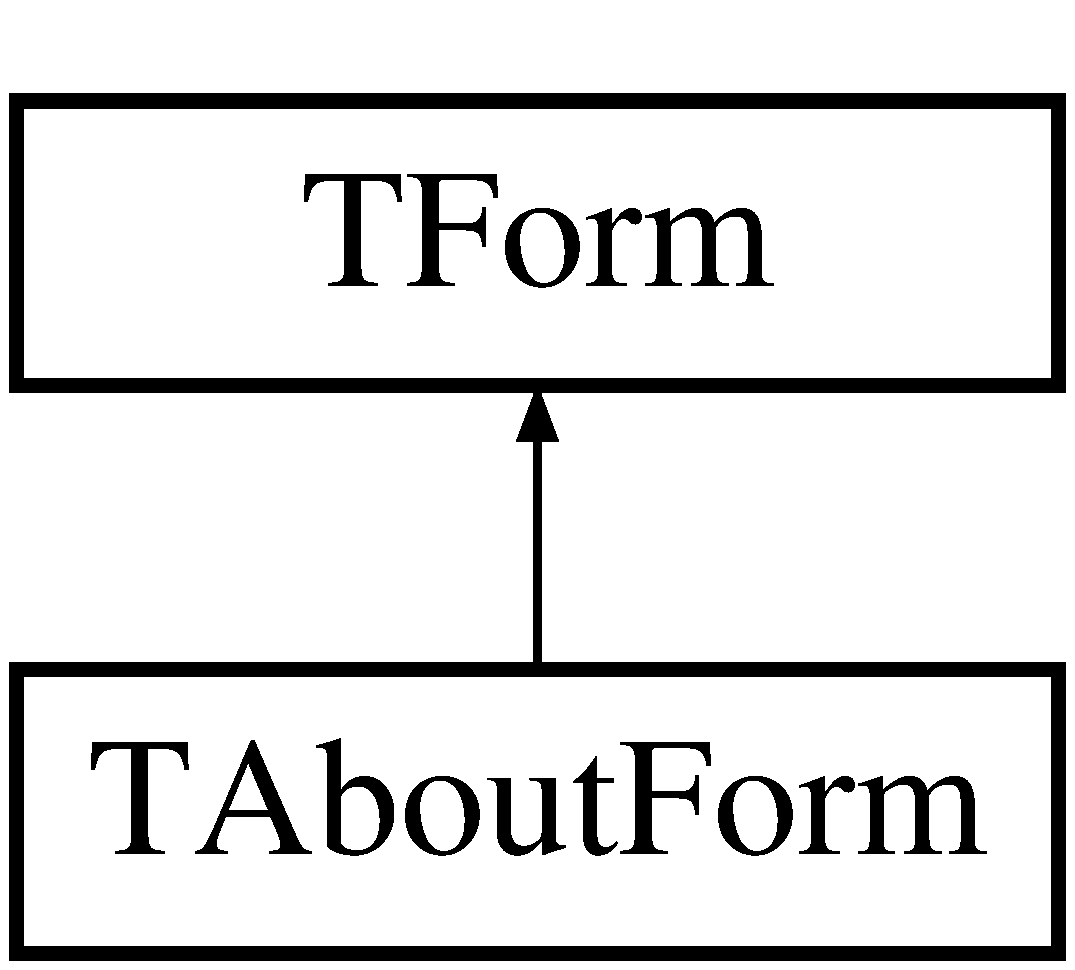
\includegraphics[height=2.000000cm]{class_t_about_form}
\end{center}
\end{figure}
\subsection*{Public Member Functions}
\begin{DoxyCompactItemize}
\item 
void \+\_\+\+\_\+fastcall \mbox{\hyperlink{class_t_about_form_ad2cb3d318c91018ed8986c8315ccd52b}{Form\+Create}} (T\+Object $\ast$Sender)
\item 
\mbox{\Hypertarget{class_t_about_form_a8e868f7264a80fda52fc8c0e8290eb3f}\label{class_t_about_form_a8e868f7264a80fda52fc8c0e8290eb3f}} 
void \+\_\+\+\_\+fastcall \mbox{\hyperlink{class_t_about_form_a8e868f7264a80fda52fc8c0e8290eb3f}{About\+Form\+Button\+Click}} (T\+Object $\ast$Sender)
\begin{DoxyCompactList}\small\item\em Closes the form. \end{DoxyCompactList}\item 
void \+\_\+\+\_\+fastcall \mbox{\hyperlink{class_t_about_form_acddaba886282fa0cb6aa0ee77520fb05}{Form\+Close}} (T\+Object $\ast$Sender, T\+Close\+Action \&Action)
\item 
\mbox{\Hypertarget{class_t_about_form_a6c7cc55bc67691c15901fdeac8bec954}\label{class_t_about_form_a6c7cc55bc67691c15901fdeac8bec954}} 
void \+\_\+\+\_\+fastcall \mbox{\hyperlink{class_t_about_form_a6c7cc55bc67691c15901fdeac8bec954}{Website\+Link\+Label\+Link\+Click}} (T\+Object $\ast$Sender, const Unicode\+String Link, T\+Sys\+Link\+Type Link\+Type)
\begin{DoxyCompactList}\small\item\em Sends the link to your default browser. \end{DoxyCompactList}\item 
\mbox{\Hypertarget{class_t_about_form_a8699bacd9787f153b92c579a4ea60871}\label{class_t_about_form_a8699bacd9787f153b92c579a4ea60871}} 
void \+\_\+\+\_\+fastcall \mbox{\hyperlink{class_t_about_form_a8699bacd9787f153b92c579a4ea60871}{Attribution1\+Link\+Label\+Link\+Click}} (T\+Object $\ast$Sender, const Unicode\+String Link, T\+Sys\+Link\+Type Link\+Type)
\begin{DoxyCompactList}\small\item\em Send the first attribution statement\textquotesingle{}s link to your default browser. \end{DoxyCompactList}\item 
\mbox{\Hypertarget{class_t_about_form_a16a26ef9958f3cdb5a0850f70d274e21}\label{class_t_about_form_a16a26ef9958f3cdb5a0850f70d274e21}} 
void \+\_\+\+\_\+fastcall \mbox{\hyperlink{class_t_about_form_a16a26ef9958f3cdb5a0850f70d274e21}{Attribution2\+Link\+Label\+Link\+Click}} (T\+Object $\ast$Sender, const Unicode\+String Link, T\+Sys\+Link\+Type Link\+Type)
\begin{DoxyCompactList}\small\item\em Send the second attribution statement\textquotesingle{}s link to your default browser. \end{DoxyCompactList}\item 
\mbox{\Hypertarget{class_t_about_form_a5f857ee166c84e44aa329cbf5e2b9400}\label{class_t_about_form_a5f857ee166c84e44aa329cbf5e2b9400}} 
\+\_\+\+\_\+fastcall \mbox{\hyperlink{class_t_about_form_a5f857ee166c84e44aa329cbf5e2b9400}{T\+About\+Form}} (T\+Component $\ast$Owner)
\begin{DoxyCompactList}\small\item\em The form constructor. \end{DoxyCompactList}\end{DoxyCompactItemize}
\subsection*{Public Attributes}
\begin{DoxyCompactItemize}
\item 
\mbox{\Hypertarget{class_t_about_form_add3f256ba4f1ed42204c0e77c0d71552}\label{class_t_about_form_add3f256ba4f1ed42204c0e77c0d71552}} 
T\+Button $\ast$ \mbox{\hyperlink{class_t_about_form_add3f256ba4f1ed42204c0e77c0d71552}{About\+Form\+Button}}
\begin{DoxyCompactList}\small\item\em The OK button. \end{DoxyCompactList}\item 
\mbox{\Hypertarget{class_t_about_form_a3c3968d0c1473343931bdd0ac25d99ab}\label{class_t_about_form_a3c3968d0c1473343931bdd0ac25d99ab}} 
T\+Image $\ast$ {\bfseries Image\+App\+Icon}
\item 
\mbox{\Hypertarget{class_t_about_form_aa188b96e0810fb8944b8e7fd7a2deea4}\label{class_t_about_form_aa188b96e0810fb8944b8e7fd7a2deea4}} 
T\+Label $\ast$ \mbox{\hyperlink{class_t_about_form_aa188b96e0810fb8944b8e7fd7a2deea4}{About\+Label\+Caption}}
\begin{DoxyCompactList}\small\item\em Version info displayed here. \end{DoxyCompactList}\item 
\mbox{\Hypertarget{class_t_about_form_a0d1afa81071159368263c6a1d1ed0c7d}\label{class_t_about_form_a0d1afa81071159368263c6a1d1ed0c7d}} 
T\+Label $\ast$ {\bfseries About\+Label\+Title}
\item 
\mbox{\Hypertarget{class_t_about_form_a809ee5cebba2a7638a31540c5b40cb28}\label{class_t_about_form_a809ee5cebba2a7638a31540c5b40cb28}} 
T\+Link\+Label $\ast$ {\bfseries Website\+Link\+Label}
\item 
\mbox{\Hypertarget{class_t_about_form_ab5ff9a28b7aa8db5c5723c8e48c4f2e1}\label{class_t_about_form_ab5ff9a28b7aa8db5c5723c8e48c4f2e1}} 
T\+Link\+Label $\ast$ {\bfseries Attribution1\+Link\+Label}
\item 
\mbox{\Hypertarget{class_t_about_form_a4f86b2ad44b1d3de8daac70528a1a3a5}\label{class_t_about_form_a4f86b2ad44b1d3de8daac70528a1a3a5}} 
T\+Link\+Label $\ast$ {\bfseries Attribution2\+Link\+Label}
\item 
\mbox{\Hypertarget{class_t_about_form_a0ff4e741e1c1c280733c3a9ccde35413}\label{class_t_about_form_a0ff4e741e1c1c280733c3a9ccde35413}} 
T\+Label $\ast$ {\bfseries Attribution1\+Label}
\item 
\mbox{\Hypertarget{class_t_about_form_adfcb216e6b70a6369dd33837e8875503}\label{class_t_about_form_adfcb216e6b70a6369dd33837e8875503}} 
T\+Label $\ast$ {\bfseries Attribution2\+Label}
\end{DoxyCompactItemize}
\subsection*{Private Member Functions}
\begin{DoxyCompactItemize}
\item 
\mbox{\Hypertarget{class_t_about_form_aae86823c5d44708f264e2c1f8cd52af1}\label{class_t_about_form_aae86823c5d44708f264e2c1f8cd52af1}} 
void \+\_\+\+\_\+fastcall \mbox{\hyperlink{class_t_about_form_aae86823c5d44708f264e2c1f8cd52af1}{Set\+About\+Caption}} ()
\begin{DoxyCompactList}\small\item\em Sets version details from the project options \textquotesingle{}Version Info\textquotesingle{} values. \end{DoxyCompactList}\end{DoxyCompactItemize}


\subsection{Detailed Description}
The small \textquotesingle{}About\textquotesingle{} box selected from the Help menu. 

\subsection{Member Function Documentation}
\mbox{\Hypertarget{class_t_about_form_acddaba886282fa0cb6aa0ee77520fb05}\label{class_t_about_form_acddaba886282fa0cb6aa0ee77520fb05}} 
\index{T\+About\+Form@{T\+About\+Form}!Form\+Close@{Form\+Close}}
\index{Form\+Close@{Form\+Close}!T\+About\+Form@{T\+About\+Form}}
\subsubsection{\texorpdfstring{Form\+Close()}{FormClose()}}
{\footnotesize\ttfamily void \+\_\+\+\_\+fastcall T\+About\+Form\+::\+Form\+Close (\begin{DoxyParamCaption}\item[{T\+Object $\ast$}]{Sender,  }\item[{T\+Close\+Action \&}]{Action }\end{DoxyParamCaption})}

Called when the form is closed

Restarts Master\+Clock if Level1\+Mode is Oper\+Mode \mbox{\Hypertarget{class_t_about_form_ad2cb3d318c91018ed8986c8315ccd52b}\label{class_t_about_form_ad2cb3d318c91018ed8986c8315ccd52b}} 
\index{T\+About\+Form@{T\+About\+Form}!Form\+Create@{Form\+Create}}
\index{Form\+Create@{Form\+Create}!T\+About\+Form@{T\+About\+Form}}
\subsubsection{\texorpdfstring{Form\+Create()}{FormCreate()}}
{\footnotesize\ttfamily void \+\_\+\+\_\+fastcall T\+About\+Form\+::\+Form\+Create (\begin{DoxyParamCaption}\item[{T\+Object $\ast$}]{Sender }\end{DoxyParamCaption})}

Called when the form is first created (by Win\+Main)

Sets the version info, then hides the form 

The documentation for this class was generated from the following files\+:\begin{DoxyCompactItemize}
\item 
About\+Unit.\+h\item 
About\+Unit.\+cpp\end{DoxyCompactItemize}

\hypertarget{class_t_action_vector_entry}{}\section{T\+Action\+Vector\+Entry Class Reference}
\label{class_t_action_vector_entry}\index{T\+Action\+Vector\+Entry@{T\+Action\+Vector\+Entry}}


Contains a single train action in a timetable -\/ repeat entry is also of this class though no train action is taken for it.  




{\ttfamily \#include $<$Train\+Unit.\+h$>$}

\subsection*{Public Member Functions}
\begin{DoxyCompactItemize}
\item 
\mbox{\Hypertarget{class_t_action_vector_entry_a2f3969c630acb3f7a346ced7a601502f}\label{class_t_action_vector_entry_a2f3969c630acb3f7a346ced7a601502f}} 
\mbox{\hyperlink{class_t_action_vector_entry_a2f3969c630acb3f7a346ced7a601502f}{T\+Action\+Vector\+Entry}} ()
\begin{DoxyCompactList}\small\item\em Constructor, sets all values to default states. \end{DoxyCompactList}\end{DoxyCompactItemize}
\subsection*{Public Attributes}
\begin{DoxyCompactItemize}
\item 
\mbox{\Hypertarget{class_t_action_vector_entry_afdc4364c8698998b3689039a32b8c148}\label{class_t_action_vector_entry_afdc4364c8698998b3689039a32b8c148}} 
Ansi\+String {\bfseries Location\+Name}
\item 
\mbox{\Hypertarget{class_t_action_vector_entry_a570ca952f6414e838be644082f02eed1}\label{class_t_action_vector_entry_a570ca952f6414e838be644082f02eed1}} 
Ansi\+String {\bfseries Command}
\item 
\mbox{\Hypertarget{class_t_action_vector_entry_a0cce6ed92eea821583a661966baae024}\label{class_t_action_vector_entry_a0cce6ed92eea821583a661966baae024}} 
Ansi\+String {\bfseries Other\+Head\+Code}
\item 
Ansi\+String \mbox{\hyperlink{class_t_action_vector_entry_ae142e8e9d3a842c9b1d81bcd4e93e291}{Non\+Repeating\+Shuttle\+Link\+Head\+Code}}
\item 
\mbox{\Hypertarget{class_t_action_vector_entry_a858aae4488b108f2e2771b1ef0e2905e}\label{class_t_action_vector_entry_a858aae4488b108f2e2771b1ef0e2905e}} 
bool \mbox{\hyperlink{class_t_action_vector_entry_a858aae4488b108f2e2771b1ef0e2905e}{Signaller\+Control}}
\begin{DoxyCompactList}\small\item\em indicates a train that is defined by the timetable as under signaller control \end{DoxyCompactList}\item 
\mbox{\Hypertarget{class_t_action_vector_entry_a43fd46452123d72efc2bd9d10008b6f1}\label{class_t_action_vector_entry_a43fd46452123d72efc2bd9d10008b6f1}} 
bool \mbox{\hyperlink{class_t_action_vector_entry_a43fd46452123d72efc2bd9d10008b6f1}{Warning}}
\begin{DoxyCompactList}\small\item\em if set triggers an alert in the warning panel when the action is reached \end{DoxyCompactList}\item 
\mbox{\Hypertarget{class_t_action_vector_entry_a5f4a663fd91b104c7f93990d79c16d1d}\label{class_t_action_vector_entry_a5f4a663fd91b104c7f93990d79c16d1d}} 
int \mbox{\hyperlink{class_t_action_vector_entry_a5f4a663fd91b104c7f93990d79c16d1d}{Number\+Of\+Repeats}}
\begin{DoxyCompactList}\small\item\em the number of repeating services \end{DoxyCompactList}\item 
\mbox{\Hypertarget{class_t_action_vector_entry_a18171f01d5e5e01242c3c672045efb28}\label{class_t_action_vector_entry_a18171f01d5e5e01242c3c672045efb28}} 
int {\bfseries Rear\+Start\+Or\+Repeat\+Mins}
\item 
int \mbox{\hyperlink{class_t_action_vector_entry_a8b84cb2a020cfb2f81a091f3bdc59ec4}{Front\+Start\+Or\+Repeat\+Digits}}
\item 
\mbox{\Hypertarget{class_t_action_vector_entry_a07850a494d4c0c71e9579c21c1910b76}\label{class_t_action_vector_entry_a07850a494d4c0c71e9579c21c1910b76}} 
T\+Date\+Time {\bfseries Event\+Time}
\item 
\mbox{\Hypertarget{class_t_action_vector_entry_a590726f5c852a19625d7fdbed22469b0}\label{class_t_action_vector_entry_a590726f5c852a19625d7fdbed22469b0}} 
T\+Date\+Time {\bfseries Arrival\+Time}
\item 
T\+Date\+Time \mbox{\hyperlink{class_t_action_vector_entry_a37c6ff0cda2672bbd60099487442fbb5}{Departure\+Time}}
\item 
\mbox{\Hypertarget{class_t_action_vector_entry_ab1d7c2bc6c0dee48c74c3dd9c325ec4d}\label{class_t_action_vector_entry_ab1d7c2bc6c0dee48c74c3dd9c325ec4d}} 
T\+Exit\+List \mbox{\hyperlink{class_t_action_vector_entry_ab1d7c2bc6c0dee48c74c3dd9c325ec4d}{Exit\+List}}
\begin{DoxyCompactList}\small\item\em the list of valid train exit Track\+Vector positions for \textquotesingle{}Fer\textquotesingle{} entries (empty to begin with) \end{DoxyCompactList}\item 
\mbox{\Hypertarget{class_t_action_vector_entry_aaa45fd77d7d5f19350a0a7a8fbc05b13}\label{class_t_action_vector_entry_aaa45fd77d7d5f19350a0a7a8fbc05b13}} 
T\+Timetable\+Format\+Type \mbox{\hyperlink{class_t_action_vector_entry_aaa45fd77d7d5f19350a0a7a8fbc05b13}{Format\+Type}}
\begin{DoxyCompactList}\small\item\em defines the timetable action type \end{DoxyCompactList}\item 
\mbox{\Hypertarget{class_t_action_vector_entry_a5de0c970525a897f8ac2cdf66004dab9}\label{class_t_action_vector_entry_a5de0c970525a897f8ac2cdf66004dab9}} 
T\+Timetable\+Location\+Type \mbox{\hyperlink{class_t_action_vector_entry_a5de0c970525a897f8ac2cdf66004dab9}{Location\+Type}}
\begin{DoxyCompactList}\small\item\em indicates where the train is when the relevant action occurs \end{DoxyCompactList}\item 
\mbox{\Hypertarget{class_t_action_vector_entry_a67b29560b218e8b8ba854d326a630682}\label{class_t_action_vector_entry_a67b29560b218e8b8ba854d326a630682}} 
T\+Timetable\+Sequence\+Type \mbox{\hyperlink{class_t_action_vector_entry_a67b29560b218e8b8ba854d326a630682}{Sequence\+Type}}
\begin{DoxyCompactList}\small\item\em indicates where in the sequence of codes the action lies \end{DoxyCompactList}\item 
\mbox{\Hypertarget{class_t_action_vector_entry_ae8efcbff8298cf829c26b0db65ffa6b3}\label{class_t_action_vector_entry_ae8efcbff8298cf829c26b0db65ffa6b3}} 
T\+Timetable\+Shuttle\+Link\+Type \mbox{\hyperlink{class_t_action_vector_entry_ae8efcbff8298cf829c26b0db65ffa6b3}{Shuttle\+Link\+Type}}
\begin{DoxyCompactList}\small\item\em indicates whether or not the action relates to a shuttle service link \end{DoxyCompactList}\item 
\mbox{\hyperlink{class_t_train_data_entry}{T\+Train\+Data\+Entry}} $\ast$ \mbox{\hyperlink{class_t_action_vector_entry_ab240a52305bd614f1921e86617687abf}{Linked\+Train\+Entry\+Ptr}}
\item 
\mbox{\hyperlink{class_t_train_data_entry}{T\+Train\+Data\+Entry}} $\ast$ \mbox{\hyperlink{class_t_action_vector_entry_a921897cd667dd8933de593e97e74a3a7}{Non\+Repeating\+Shuttle\+Link\+Entry\+Ptr}}
\end{DoxyCompactItemize}


\subsection{Detailed Description}
Contains a single train action in a timetable -\/ repeat entry is also of this class though no train action is taken for it. 

\subsection{Member Data Documentation}
\mbox{\Hypertarget{class_t_action_vector_entry_a37c6ff0cda2672bbd60099487442fbb5}\label{class_t_action_vector_entry_a37c6ff0cda2672bbd60099487442fbb5}} 
\index{T\+Action\+Vector\+Entry@{T\+Action\+Vector\+Entry}!Departure\+Time@{Departure\+Time}}
\index{Departure\+Time@{Departure\+Time}!T\+Action\+Vector\+Entry@{T\+Action\+Vector\+Entry}}
\subsubsection{\texorpdfstring{Departure\+Time}{DepartureTime}}
{\footnotesize\ttfamily T\+Date\+Time T\+Action\+Vector\+Entry\+::\+Departure\+Time}

relevant times at which the action is timetabled, zeroed on creation so change to -\/1 as a marker for \textquotesingle{}not set\textquotesingle{} \mbox{\Hypertarget{class_t_action_vector_entry_a8b84cb2a020cfb2f81a091f3bdc59ec4}\label{class_t_action_vector_entry_a8b84cb2a020cfb2f81a091f3bdc59ec4}} 
\index{T\+Action\+Vector\+Entry@{T\+Action\+Vector\+Entry}!Front\+Start\+Or\+Repeat\+Digits@{Front\+Start\+Or\+Repeat\+Digits}}
\index{Front\+Start\+Or\+Repeat\+Digits@{Front\+Start\+Or\+Repeat\+Digits}!T\+Action\+Vector\+Entry@{T\+Action\+Vector\+Entry}}
\subsubsection{\texorpdfstring{Front\+Start\+Or\+Repeat\+Digits}{FrontStartOrRepeatDigits}}
{\footnotesize\ttfamily int T\+Action\+Vector\+Entry\+::\+Front\+Start\+Or\+Repeat\+Digits}

dual-\/purpose variables used for the Track\+Vector\+Positions of the rear and front train starting elements (for Snt) or for repeat minute \& digit values in repeat entries \mbox{\Hypertarget{class_t_action_vector_entry_ab240a52305bd614f1921e86617687abf}\label{class_t_action_vector_entry_ab240a52305bd614f1921e86617687abf}} 
\index{T\+Action\+Vector\+Entry@{T\+Action\+Vector\+Entry}!Linked\+Train\+Entry\+Ptr@{Linked\+Train\+Entry\+Ptr}}
\index{Linked\+Train\+Entry\+Ptr@{Linked\+Train\+Entry\+Ptr}!T\+Action\+Vector\+Entry@{T\+Action\+Vector\+Entry}}
\subsubsection{\texorpdfstring{Linked\+Train\+Entry\+Ptr}{LinkedTrainEntryPtr}}
{\footnotesize\ttfamily \mbox{\hyperlink{class_t_train_data_entry}{T\+Train\+Data\+Entry}}$\ast$ T\+Action\+Vector\+Entry\+::\+Linked\+Train\+Entry\+Ptr}

link pointer for use between fsp/rsp \& Sfs; Fjo \& jbo; Fns \& Sns; \& all shuttle to shuttle links \mbox{\Hypertarget{class_t_action_vector_entry_a921897cd667dd8933de593e97e74a3a7}\label{class_t_action_vector_entry_a921897cd667dd8933de593e97e74a3a7}} 
\index{T\+Action\+Vector\+Entry@{T\+Action\+Vector\+Entry}!Non\+Repeating\+Shuttle\+Link\+Entry\+Ptr@{Non\+Repeating\+Shuttle\+Link\+Entry\+Ptr}}
\index{Non\+Repeating\+Shuttle\+Link\+Entry\+Ptr@{Non\+Repeating\+Shuttle\+Link\+Entry\+Ptr}!T\+Action\+Vector\+Entry@{T\+Action\+Vector\+Entry}}
\subsubsection{\texorpdfstring{Non\+Repeating\+Shuttle\+Link\+Entry\+Ptr}{NonRepeatingShuttleLinkEntryPtr}}
{\footnotesize\ttfamily \mbox{\hyperlink{class_t_train_data_entry}{T\+Train\+Data\+Entry}}$\ast$ T\+Action\+Vector\+Entry\+::\+Non\+Repeating\+Shuttle\+Link\+Entry\+Ptr}

pointer used by shuttles for the non-\/shuttle train links, in \& out, the corresponding non-\/shuttle linked trains use Linked\+Train\+Entry\+Ptr \mbox{\Hypertarget{class_t_action_vector_entry_ae142e8e9d3a842c9b1d81bcd4e93e291}\label{class_t_action_vector_entry_ae142e8e9d3a842c9b1d81bcd4e93e291}} 
\index{T\+Action\+Vector\+Entry@{T\+Action\+Vector\+Entry}!Non\+Repeating\+Shuttle\+Link\+Head\+Code@{Non\+Repeating\+Shuttle\+Link\+Head\+Code}}
\index{Non\+Repeating\+Shuttle\+Link\+Head\+Code@{Non\+Repeating\+Shuttle\+Link\+Head\+Code}!T\+Action\+Vector\+Entry@{T\+Action\+Vector\+Entry}}
\subsubsection{\texorpdfstring{Non\+Repeating\+Shuttle\+Link\+Head\+Code}{NonRepeatingShuttleLinkHeadCode}}
{\footnotesize\ttfamily Ansi\+String T\+Action\+Vector\+Entry\+::\+Non\+Repeating\+Shuttle\+Link\+Head\+Code}

string values for timetabled action entries, null on creation 

The documentation for this class was generated from the following file\+:\begin{DoxyCompactItemize}
\item 
Train\+Unit.\+h\end{DoxyCompactItemize}

\hypertarget{class_t_track_1_1_t_active_level_crossing}{}\doxysection{T\+Track\+::T\+Active\+Level\+Crossing Class Reference}
\label{class_t_track_1_1_t_active_level_crossing}\index{TTrack::TActiveLevelCrossing@{TTrack::TActiveLevelCrossing}}


{\ttfamily \#include $<$Track\+Unit.\+h$>$}

\doxysubsection*{Public Member Functions}
\begin{DoxyCompactItemize}
\item 
\mbox{\Hypertarget{class_t_track_1_1_t_active_level_crossing_adc74855a4f0cb115cef8be85b1288f15}\label{class_t_track_1_1_t_active_level_crossing_adc74855a4f0cb115cef8be85b1288f15}} 
\mbox{\hyperlink{class_t_track_1_1_t_active_level_crossing_adc74855a4f0cb115cef8be85b1288f15}{T\+Active\+Level\+Crossing\+::\+T\+Active\+Level\+Crossing}} ()
\begin{DoxyCompactList}\small\item\em constructor, sets default values \end{DoxyCompactList}\end{DoxyCompactItemize}
\doxysubsection*{Public Attributes}
\begin{DoxyCompactItemize}
\item 
\mbox{\Hypertarget{class_t_track_1_1_t_active_level_crossing_ab673508a424b72287259591f31e309fd}\label{class_t_track_1_1_t_active_level_crossing_ab673508a424b72287259591f31e309fd}} 
bool \mbox{\hyperlink{class_t_track_1_1_t_active_level_crossing_ab673508a424b72287259591f31e309fd}{Consec\+Signals}}
\begin{DoxyCompactList}\small\item\em route type -\/ 0 = nonsignals, 1 = preferred direction (can\textquotesingle{}t have autosigs) \end{DoxyCompactList}\item 
\mbox{\Hypertarget{class_t_track_1_1_t_active_level_crossing_a1cdc06cbcf27faf07f7a653a51cd661e}\label{class_t_track_1_1_t_active_level_crossing_a1cdc06cbcf27faf07f7a653a51cd661e}} 
bool \mbox{\hyperlink{class_t_track_1_1_t_active_level_crossing_a1cdc06cbcf27faf07f7a653a51cd661e}{Train\+Passed}}
\begin{DoxyCompactList}\small\item\em marker that is set when a train is present on one of the elements of the LC -\/ used to provide a 3 minute penalty allowance \end{DoxyCompactList}\item 
\mbox{\Hypertarget{class_t_track_1_1_t_active_level_crossing_ae6a3eed6fc68f1e65a59a3da36a3d4cb}\label{class_t_track_1_1_t_active_level_crossing_ae6a3eed6fc68f1e65a59a3da36a3d4cb}} 
T\+Barrier\+State \mbox{\hyperlink{class_t_track_1_1_t_active_level_crossing_ae6a3eed6fc68f1e65a59a3da36a3d4cb}{Barrier\+State}}
\begin{DoxyCompactList}\small\item\em state of barriers \end{DoxyCompactList}\item 
\mbox{\Hypertarget{class_t_track_1_1_t_active_level_crossing_af45c2e8c0f427b23e655cdce00cebbb8}\label{class_t_track_1_1_t_active_level_crossing_af45c2e8c0f427b23e655cdce00cebbb8}} 
float \mbox{\hyperlink{class_t_track_1_1_t_active_level_crossing_af45c2e8c0f427b23e655cdce00cebbb8}{Change\+Duration}}
\begin{DoxyCompactList}\small\item\em duration of the level crossing changing period \end{DoxyCompactList}\item 
\mbox{\Hypertarget{class_t_track_1_1_t_active_level_crossing_aaca7018cee472ba2b5df1589caa071f7}\label{class_t_track_1_1_t_active_level_crossing_aaca7018cee472ba2b5df1589caa071f7}} 
int \mbox{\hyperlink{class_t_track_1_1_t_active_level_crossing_aaca7018cee472ba2b5df1589caa071f7}{Base\+Element\+Speed\+Tag}}
\begin{DoxyCompactList}\small\item\em Speed\+Tag value for the base element of a level crossing. \end{DoxyCompactList}\item 
\mbox{\Hypertarget{class_t_track_1_1_t_active_level_crossing_ad935a5012ee1d5bee8767e1c634dafbf}\label{class_t_track_1_1_t_active_level_crossing_ad935a5012ee1d5bee8767e1c634dafbf}} 
int \mbox{\hyperlink{class_t_track_1_1_t_active_level_crossing_ad935a5012ee1d5bee8767e1c634dafbf}{H\+Loc}}
\begin{DoxyCompactList}\small\item\em H\+Loc value for found level crossing element. \end{DoxyCompactList}\item 
\mbox{\Hypertarget{class_t_track_1_1_t_active_level_crossing_afabdf5593ed4d0f2f406aac52d7b4fb4}\label{class_t_track_1_1_t_active_level_crossing_afabdf5593ed4d0f2f406aac52d7b4fb4}} 
int \mbox{\hyperlink{class_t_track_1_1_t_active_level_crossing_afabdf5593ed4d0f2f406aac52d7b4fb4}{V\+Loc}}
\begin{DoxyCompactList}\small\item\em V\+Loc value for found level crossing element. \end{DoxyCompactList}\item 
\mbox{\Hypertarget{class_t_track_1_1_t_active_level_crossing_a428974b7cd394ee22cfbcae541cd262b}\label{class_t_track_1_1_t_active_level_crossing_a428974b7cd394ee22cfbcae541cd262b}} 
T\+Date\+Time \mbox{\hyperlink{class_t_track_1_1_t_active_level_crossing_a428974b7cd394ee22cfbcae541cd262b}{Start\+Time}}
\begin{DoxyCompactList}\small\item\em stores the starting time for level crossing changing \end{DoxyCompactList}\end{DoxyCompactItemize}


\doxysubsection{Detailed Description}
Values for level crossings either changing state or with barriers down

All L\+Cs begin with barriers raised. i.\+e. closed to trains, that is the normal state. When a route is set through an LC nothing happens until the route is set, then an active LC object is created by Set\+L\+C\+Change\+Values (called by Convertand\+Add.... for lowering barriers) and added to the Changing\+L\+C\+Vector. Once created \textquotesingle{}Flashing\+Graphics\textquotesingle{} takes care of the flashing, until the duration is reached. While flashing no further routes can be set through that LC and the first route can\textquotesingle{}t be cancelled, hence the flashing only needs to cater for plotting the route on the one track that started the barrier lowering. When the duration is reached, the object is transferred to a new vector Barriers\+Down\+Vector, after the Start\+Time has been reset (to time the period for which the barriers are down -\/ penalties are given for $>$ 3 minutes), Barrier\+State changed to Down, and the object erased from Changing\+L\+C\+Vector. When there is no route through an LC and no train on the track then the barriers are raised -\/ in Clock\+Timer2 -\/ when the Barriers\+Down\+Vector object is copied back to Changing\+L\+C\+Vector with a new Start\+Time, Barrier\+State and Change\+Duration. Again Flashing\+Graphics takes care of the flashing until the duration is reached, when the object is erased from the vector and the LC reverts to its normal (barriers raised) state. 

The documentation for this class was generated from the following file\+:\begin{DoxyCompactItemize}
\item 
Track\+Unit.\+h\end{DoxyCompactItemize}

\hypertarget{class_t_all_routes}{}\section{T\+All\+Routes Class Reference}
\label{class_t_all_routes}\index{T\+All\+Routes@{T\+All\+Routes}}


Handles data and functions relating to all routes on the railway.  




{\ttfamily \#include $<$Track\+Unit.\+h$>$}

\subsection*{Classes}
\begin{DoxyCompactItemize}
\item 
class \mbox{\hyperlink{class_t_all_routes_1_1_t_callon_entry}{T\+Callon\+Entry}}
\begin{DoxyCompactList}\small\item\em Used to store relevant values when a call-\/on found, ready for plotting an unrestricted route. \end{DoxyCompactList}\item 
class \mbox{\hyperlink{class_t_all_routes_1_1_t_locked_route_class}{T\+Locked\+Route\+Class}}
\begin{DoxyCompactList}\small\item\em Handles routes that are locked because of approaching trains. \end{DoxyCompactList}\end{DoxyCompactItemize}
\subsection*{Public Types}
\begin{DoxyCompactItemize}
\item 
\mbox{\Hypertarget{class_t_all_routes_af94f31040cc7692c777123c609d4cbd6}\label{class_t_all_routes_af94f31040cc7692c777123c609d4cbd6}} 
enum {\bfseries T\+Route\+Type} \{ {\bfseries No\+Route}, 
{\bfseries Not\+Auto\+Sigs\+Route}, 
{\bfseries Auto\+Sigs\+Route}
 \}
\item 
\mbox{\Hypertarget{class_t_all_routes_a34636f74b522ec911900fce48ea6667c}\label{class_t_all_routes_a34636f74b522ec911900fce48ea6667c}} 
typedef std\+::vector$<$ \mbox{\hyperlink{class_t_one_route}{T\+One\+Route}} $>$ \mbox{\hyperlink{class_t_all_routes_a34636f74b522ec911900fce48ea6667c}{T\+All\+Routes\+Vector}}
\begin{DoxyCompactList}\small\item\em the vector class that holds all the railway routes \end{DoxyCompactList}\item 
\mbox{\Hypertarget{class_t_all_routes_a863ba954ac5b7e2197ae1074cc7e268b}\label{class_t_all_routes_a863ba954ac5b7e2197ae1074cc7e268b}} 
typedef std\+::vector$<$ \mbox{\hyperlink{class_t_one_route}{T\+One\+Route}} $>$\+::iterator {\bfseries T\+All\+Routes\+Vector\+Iterator}
\item 
\mbox{\Hypertarget{class_t_all_routes_a00c2d57382ed6560f1c611bdfddc3a6f}\label{class_t_all_routes_a00c2d57382ed6560f1c611bdfddc3a6f}} 
typedef std\+::vector$<$ \mbox{\hyperlink{class_t_all_routes_1_1_t_locked_route_class}{T\+Locked\+Route\+Class}} $>$ \mbox{\hyperlink{class_t_all_routes_a00c2d57382ed6560f1c611bdfddc3a6f}{T\+Locked\+Route\+Vector}}
\begin{DoxyCompactList}\small\item\em the vector class that holds all locked routes \end{DoxyCompactList}\item 
\mbox{\Hypertarget{class_t_all_routes_ac58b6335a806c347545f73f680b45afa}\label{class_t_all_routes_ac58b6335a806c347545f73f680b45afa}} 
typedef std\+::vector$<$ \mbox{\hyperlink{class_t_all_routes_1_1_t_locked_route_class}{T\+Locked\+Route\+Class}} $>$\+::iterator {\bfseries T\+Locked\+Route\+Vector\+Iterator}
\item 
typedef std\+::pair$<$ int, unsigned int $>$ \mbox{\hyperlink{class_t_all_routes_a159a7d547e3d435d109a36cb41193a78}{T\+Route\+Element\+Pair}}
\item 
typedef std\+::multimap$<$ T\+H\+V\+Pair, \mbox{\hyperlink{class_t_all_routes_a159a7d547e3d435d109a36cb41193a78}{T\+Route\+Element\+Pair}}, \mbox{\hyperlink{class_t_map_comp}{T\+Map\+Comp}} $>$ \mbox{\hyperlink{class_t_all_routes_a1d2aa3032df6e13d1f6f1a93f96157c6}{T\+Route2\+Multi\+Map}}
\item 
\mbox{\Hypertarget{class_t_all_routes_a44189363afe506f3f87c3cb6f81c539b}\label{class_t_all_routes_a44189363afe506f3f87c3cb6f81c539b}} 
typedef T\+Route2\+Multi\+Map\+::iterator {\bfseries T\+Route2\+Multi\+Map\+Iterator}
\item 
\mbox{\Hypertarget{class_t_all_routes_a993331007a31dae38f2d81afe0796ef4}\label{class_t_all_routes_a993331007a31dae38f2d81afe0796ef4}} 
typedef std\+::pair$<$ T\+H\+V\+Pair, \mbox{\hyperlink{class_t_all_routes_a159a7d547e3d435d109a36cb41193a78}{T\+Route\+Element\+Pair}} $>$ {\bfseries T\+Route2\+Multi\+Map\+Entry}
\end{DoxyCompactItemize}
\subsection*{Public Member Functions}
\begin{DoxyCompactItemize}
\item 
\mbox{\Hypertarget{class_t_all_routes_a438b71f3afbc2c8adb45b47f69cb3bb9}\label{class_t_all_routes_a438b71f3afbc2c8adb45b47f69cb3bb9}} 
unsigned int \mbox{\hyperlink{class_t_all_routes_a438b71f3afbc2c8adb45b47f69cb3bb9}{All\+Routes\+Size}} () const
\begin{DoxyCompactList}\small\item\em Returns the number of routes in the railway. \end{DoxyCompactList}\item 
\mbox{\Hypertarget{class_t_all_routes_a30042b2492dc00cec8e5cba68c446efb}\label{class_t_all_routes_a30042b2492dc00cec8e5cba68c446efb}} 
void \mbox{\hyperlink{class_t_all_routes_a30042b2492dc00cec8e5cba68c446efb}{All\+Routes\+Clear}} ()
\begin{DoxyCompactList}\small\item\em Erases all routes from All\+Routes\+Vector and from Route2\+Multi\+Map. \end{DoxyCompactList}\item 
\mbox{\Hypertarget{class_t_all_routes_a12eedbd538ea1c2d3f204e5f2f62e1cd}\label{class_t_all_routes_a12eedbd538ea1c2d3f204e5f2f62e1cd}} 
bool \mbox{\hyperlink{class_t_all_routes_a12eedbd538ea1c2d3f204e5f2f62e1cd}{Check\+For\+Looping\+Route}} (int Caller, int End\+Position, int End\+X\+Link\+Pos, int Start\+Position)
\begin{DoxyCompactList}\small\item\em Functions defined in .cpp file. \end{DoxyCompactList}\item 
\mbox{\Hypertarget{class_t_all_routes_ad151a9c7a0ad304f0f5c5c6b523ffb2e}\label{class_t_all_routes_ad151a9c7a0ad304f0f5c5c6b523ffb2e}} 
bool \mbox{\hyperlink{class_t_all_routes_ad151a9c7a0ad304f0f5c5c6b523ffb2e}{Check\+Routes}} (int Caller, int Number\+Of\+Active\+Elements, std\+::ifstream \&In\+File)
\begin{DoxyCompactList}\small\item\em Performs an integrity check on the routes stored in a session file and returns false if there is an error. \end{DoxyCompactList}\item 
bool \mbox{\hyperlink{class_t_all_routes_a2341a7e860e716e60b733f45814e4499}{Diagonal\+Fouled\+By\+Route\+Or\+Train}} (int Caller, int H\+Loc, int V\+Loc, int Diagonal\+Link\+Number)
\item 
\mbox{\Hypertarget{class_t_all_routes_ae3fb64509afc46d5871c7843c7769f88}\label{class_t_all_routes_ae3fb64509afc46d5871c7843c7769f88}} 
bool \mbox{\hyperlink{class_t_all_routes_ae3fb64509afc46d5871c7843c7769f88}{Diagonal\+Fouled\+By\+Route}} (int Caller, int H\+Loc, int V\+Loc, int Diagonal\+Link\+Number)
\begin{DoxyCompactList}\small\item\em As above but only checks for a route (may or may not be a train present (new at v1.\+2.\+0) \end{DoxyCompactList}\item 
bool \mbox{\hyperlink{class_t_all_routes_ac80a3ae43f749d401f470de711e8e4b0}{Find\+Route\+Number\+From\+Route2\+Multi\+Map\+No\+Errors}} (int Caller, int H\+Loc, int V\+Loc, int E\+Link, int \&Route\+Number)
\item 
bool \mbox{\hyperlink{class_t_all_routes_a0f3313fe1870b98a63cbc0deda000d4e}{Get\+All\+Routes\+Truncate\+Element}} (int Caller, int H\+Loc, int V\+Loc, bool Consec\+Signals\+Route)
\item 
bool \mbox{\hyperlink{class_t_all_routes_aa92b37f73176fcf3454688bb15b9f64c}{Is\+Element\+In\+Locked\+Route\+Get\+Pref\+Dir\+Element\+Get\+Locked\+Vector\+Number}} (int Caller, int Track\+Vector\+Position, int X\+Link\+Pos, \mbox{\hyperlink{class_t_pref_dir_element}{T\+Pref\+Dir\+Element}} \&Pref\+Dir\+Element, int \&Locked\+Vector\+Number)
\item 
\mbox{\Hypertarget{class_t_all_routes_ac0c25f0bd613ff645dab243f1eb8b593}\label{class_t_all_routes_ac0c25f0bd613ff645dab243f1eb8b593}} 
bool \mbox{\hyperlink{class_t_all_routes_ac0c25f0bd613ff645dab243f1eb8b593}{Is\+There\+A\+Route\+At\+I\+D\+Number}} (int Caller, \mbox{\hyperlink{class_i_d_int}{I\+D\+Int}} Route\+ID)
\begin{DoxyCompactList}\small\item\em Returns true if there is a route with the given ID number -\/ added at v1.\+3.\+1 (see function for details) \end{DoxyCompactList}\item 
\mbox{\Hypertarget{class_t_all_routes_adadd08bb4cbbcaeba918f20c6c103a39}\label{class_t_all_routes_adadd08bb4cbbcaeba918f20c6c103a39}} 
bool \mbox{\hyperlink{class_t_all_routes_adadd08bb4cbbcaeba918f20c6c103a39}{Load\+Routes}} (int Caller, std\+::ifstream \&In\+File)
\begin{DoxyCompactList}\small\item\em Loads the routes from a session file. \end{DoxyCompactList}\item 
bool \mbox{\hyperlink{class_t_all_routes_a38ede0231e26c62498999d1873d547a2}{Route\+Locking\+Required}} (int Caller, int Route\+Number, int Route\+Truncate\+Position)
\item 
bool \mbox{\hyperlink{class_t_all_routes_aace498b67ccef13364a1afa1f5f15311}{Track\+Is\+In\+A\+Route}} (int Caller, int Track\+Vector\+Position, int Link\+Pos)
\item 
\mbox{\Hypertarget{class_t_all_routes_a1913c6b3db0107874816d94a4d77e7a8}\label{class_t_all_routes_a1913c6b3db0107874816d94a4d77e7a8}} 
int \mbox{\hyperlink{class_t_all_routes_a1913c6b3db0107874816d94a4d77e7a8}{Get\+Route\+Vector\+Number}} (int Caller, \mbox{\hyperlink{class_i_d_int}{I\+D\+Int}} Route\+ID)
\begin{DoxyCompactList}\small\item\em Returns a route\textquotesingle{}s position in All\+Routes\+Vector from its ID, throws an error if a matching route isn\textquotesingle{}t found. \end{DoxyCompactList}\item 
const \mbox{\hyperlink{class_t_one_route}{T\+One\+Route}} \& \mbox{\hyperlink{class_t_all_routes_a7d9f820738af6314f2b9a4a1f52bb64a}{Get\+Fixed\+Route\+At}} (int Caller, int At) const
\item 
\mbox{\Hypertarget{class_t_all_routes_a415c16a43e8e997c82226987e7bffc59}\label{class_t_all_routes_a415c16a43e8e997c82226987e7bffc59}} 
const \mbox{\hyperlink{class_t_one_route}{T\+One\+Route}} \& \mbox{\hyperlink{class_t_all_routes_a415c16a43e8e997c82226987e7bffc59}{Get\+Fixed\+Route\+At\+I\+D\+Number}} (int Caller, \mbox{\hyperlink{class_i_d_int}{I\+D\+Int}} Route\+ID) const
\begin{DoxyCompactList}\small\item\em Returns a constant reference to the route with ID number Route\+ID. If no route is found with that ID an error is thrown. \end{DoxyCompactList}\item 
\mbox{\hyperlink{class_t_one_route}{T\+One\+Route}} \& \mbox{\hyperlink{class_t_all_routes_a8b522eb0d7aa415c3648d464c2885484}{Get\+Modifiable\+Route\+At}} (int Caller, int At)
\item 
\mbox{\hyperlink{class_t_one_route}{T\+One\+Route}} \& \mbox{\hyperlink{class_t_all_routes_a22bbb69a96356c26848fe9c6b154f387}{Get\+Modifiable\+Route\+At\+I\+D\+Number}} (int Caller, \mbox{\hyperlink{class_i_d_int}{I\+D\+Int}} Route\+ID)
\item 
\mbox{\hyperlink{class_t_all_routes_a159a7d547e3d435d109a36cb41193a78}{T\+Route\+Element\+Pair}} \mbox{\hyperlink{class_t_all_routes_a73d2c20327947600e5af57f908359343}{Find\+Route\+Pair\+From\+Route2\+Multi\+Map}} (int Caller, int H\+Loc, int V\+Loc, int E\+Link, T\+Route2\+Multi\+Map\+Iterator \&Route2\+Multi\+Map\+Iterator)
\item 
\mbox{\hyperlink{class_t_all_routes_a159a7d547e3d435d109a36cb41193a78}{T\+Route\+Element\+Pair}} \mbox{\hyperlink{class_t_all_routes_a7eda7a4b535c7538e217bbbc4d878071}{Get\+Route\+Element\+Data\+From\+Route2\+Multi\+Map}} (int Caller, int H\+Loc, int V\+Loc, \mbox{\hyperlink{class_t_all_routes_a159a7d547e3d435d109a36cb41193a78}{T\+Route\+Element\+Pair}} \&Second\+Pair)
\item 
T\+Route\+Type \mbox{\hyperlink{class_t_all_routes_afbb161c646677f13755041b895a23982}{Get\+Route\+Type\+And\+Graphics}} (int Caller, int Track\+Vector\+Position, int Link\+Pos, Graphics\+::\+T\+Bitmap $\ast$\&E\+X\+Graphic\+Ptr, Graphics\+::\+T\+Bitmap $\ast$\&Entry\+Direction\+Graphic\+Ptr)
\item 
T\+Route\+Type \mbox{\hyperlink{class_t_all_routes_a0a9ccbc84687f85806115877aa86dcfd}{Get\+Route\+Type\+And\+Number}} (int Caller, int Track\+Vector\+Position, int Link\+Pos, int \&Route\+Number)
\item 
void \mbox{\hyperlink{class_t_all_routes_a6eaa33fa8e8dcb44d0671be5889305a9}{Add\+Route\+Element}} (int Caller, int H\+Loc, int V\+Loc, int E\+Link, int Route\+Number, \mbox{\hyperlink{class_t_pref_dir_element}{T\+Pref\+Dir\+Element}} Route\+Element)
\item 
void \mbox{\hyperlink{class_t_all_routes_a54e5483e7b01daf50436e3dcc8794e77}{Check\+Map\+And\+Routes}} (int Caller)
\item 
void \mbox{\hyperlink{class_t_all_routes_ab23a53bd95aeb951108a004735b9a45e}{Clear\+Route\+During\+Route\+Building\+At}} (int Caller, int Route\+Number)
\item 
void \mbox{\hyperlink{class_t_all_routes_a5ebf1d3fbba09f98acc23b7d18822e9e}{Decrement\+Route\+Element\+Numbers\+In\+Route2\+Multi\+Map}} (int Caller, int Route\+Number, unsigned int Erased\+Element\+Number)
\item 
void \mbox{\hyperlink{class_t_all_routes_a5b18fe89f84962fca0a86063043b2a75}{Decrement\+Route\+Numbers\+In\+Route2\+Multi\+Map}} (int Caller, int Route\+Number)
\item 
\mbox{\Hypertarget{class_t_all_routes_af0a34aa05027527d256566ae52600583}\label{class_t_all_routes_af0a34aa05027527d256566ae52600583}} 
void \mbox{\hyperlink{class_t_all_routes_af0a34aa05027527d256566ae52600583}{Mark\+All\+Routes}} (int Caller, \mbox{\hyperlink{class_t_display}{T\+Display}} $\ast$Disp)
\begin{DoxyCompactList}\small\item\em Calls Pref\+Dir\+Marker for all routes, with Route\+Call set to identify a route call, and Building\+Pref\+Dir false. \end{DoxyCompactList}\item 
\mbox{\Hypertarget{class_t_all_routes_aacbc3765d695c99cf64ad2826792508f}\label{class_t_all_routes_aacbc3765d695c99cf64ad2826792508f}} 
void \mbox{\hyperlink{class_t_all_routes_aacbc3765d695c99cf64ad2826792508f}{Remove\+Route\+Element}} (int Caller, int H\+Loc, int V\+Loc, int E\+Link)
\begin{DoxyCompactList}\small\item\em Erases the route element from Route2\+Multi\+Map and from the Pref\+Dir\+Vector. \end{DoxyCompactList}\item 
\mbox{\Hypertarget{class_t_all_routes_a6f4b576505cc7f2384edd60ffabddc8f}\label{class_t_all_routes_a6f4b576505cc7f2384edd60ffabddc8f}} 
void \mbox{\hyperlink{class_t_all_routes_a6f4b576505cc7f2384edd60ffabddc8f}{Route2\+Multi\+Map\+Insert}} (int Caller, int H\+Loc, int V\+Loc, int E\+Link\+In, int Route\+Number, unsigned int Route\+Element\+Number)
\begin{DoxyCompactList}\small\item\em Insert an entry in Route2\+Multi\+Map. Called by \mbox{\hyperlink{class_t_all_routes_a6eaa33fa8e8dcb44d0671be5889305a9}{T\+All\+Routes\+::\+Add\+Route\+Element}}. \end{DoxyCompactList}\item 
\mbox{\Hypertarget{class_t_all_routes_a4eeafc071c52e16eb1cbe5fb14b2561f}\label{class_t_all_routes_a4eeafc071c52e16eb1cbe5fb14b2561f}} 
void \mbox{\hyperlink{class_t_all_routes_a4eeafc071c52e16eb1cbe5fb14b2561f}{Save\+Routes}} (int Caller, std\+::ofstream \&Out\+File)
\begin{DoxyCompactList}\small\item\em Save railway route information to a session file or an error file. \end{DoxyCompactList}\item 
\mbox{\Hypertarget{class_t_all_routes_ac6bd39457747eaa96476a8a87df15ac2}\label{class_t_all_routes_ac6bd39457747eaa96476a8a87df15ac2}} 
void \mbox{\hyperlink{class_t_all_routes_ac6bd39457747eaa96476a8a87df15ac2}{Set\+All\+Rearwards\+Signals}} (int Caller, int Attribute, int Route\+Number, int Route\+Start\+Position)
\begin{DoxyCompactList}\small\item\em Set rearwards signals from the specified route starting position. \end{DoxyCompactList}\item 
void \mbox{\hyperlink{class_t_all_routes_a2ab882d5be1966d8a492d13886531c45}{Set\+Trailing\+Signals\+On\+Auto\+Sigs\+Route}} (int Caller, int Track\+Vector\+Position, int X\+Link\+Pos)
\item 
void \mbox{\hyperlink{class_t_all_routes_a18177a40331bb96bbec791245b541f47}{Set\+Trailing\+Signals\+On\+Continuation\+Route}} (int Caller, int Route\+Number, int Access\+Number)
\item 
void \mbox{\hyperlink{class_t_all_routes_af70c07d73f0b62ed85bbebc5451d009c}{Store\+One\+Route}} (int Caller, \mbox{\hyperlink{class_t_one_route}{T\+One\+Route}} $\ast$Route)
\item 
void \mbox{\hyperlink{class_t_all_routes_a7bf52152ec8f71a9aa78ad4dc4f80c65}{Store\+One\+Route\+After\+Session\+Load}} (int Caller, \mbox{\hyperlink{class_t_one_route}{T\+One\+Route}} $\ast$Route)
\item 
void \mbox{\hyperlink{class_t_all_routes_a7c9ca14ec6116983b505f0a451dd078f}{Write\+All\+Routes\+To\+Image}} (int Caller, Graphics\+::\+T\+Bitmap $\ast$Bitmap)
\item 
\mbox{\Hypertarget{class_t_all_routes_ad562b9a2301042e109db1a895235e36f}\label{class_t_all_routes_ad562b9a2301042e109db1a895235e36f}} 
\mbox{\hyperlink{class_t_all_routes_ad562b9a2301042e109db1a895235e36f}{T\+All\+Routes}} ()
\begin{DoxyCompactList}\small\item\em Constructor. \end{DoxyCompactList}\end{DoxyCompactItemize}
\subsection*{Public Attributes}
\begin{DoxyCompactItemize}
\item 
enum T\+All\+Routes\+::\+T\+Route\+Type \mbox{\hyperlink{class_t_all_routes_a418f6235db60f6f41c56aede07b5fe24}{Route\+Type}}
\begin{DoxyCompactList}\small\item\em or no route at all (where this is used there is no need to distinguish between preferred direction and unrestricted routes) \end{DoxyCompactList}\item 
\mbox{\Hypertarget{class_t_all_routes_a3993d52ba2a60f04572838e2cbd78bbf}\label{class_t_all_routes_a3993d52ba2a60f04572838e2cbd78bbf}} 
std\+::vector$<$ \mbox{\hyperlink{class_t_all_routes_1_1_t_callon_entry}{T\+Callon\+Entry}} $>$ \mbox{\hyperlink{class_t_all_routes_a3993d52ba2a60f04572838e2cbd78bbf}{Callon\+Vector}}
\begin{DoxyCompactList}\small\item\em the store of all call-\/on entries \end{DoxyCompactList}\item 
bool \mbox{\hyperlink{class_t_all_routes_a961a443309f2ea74dc4c24b5a94fd8b6}{Locked\+Route\+Found\+During\+Route\+Building}}
\item 
\mbox{\Hypertarget{class_t_all_routes_a932ef101ca1ede0b8b4c71a697c910fc}\label{class_t_all_routes_a932ef101ca1ede0b8b4c71a697c910fc}} 
int {\bfseries Locked\+Route\+Last\+X\+Link\+Pos}
\item 
\mbox{\Hypertarget{class_t_all_routes_a81d0fa90e6eccdcf7df2efadb762ae80}\label{class_t_all_routes_a81d0fa90e6eccdcf7df2efadb762ae80}} 
unsigned int {\bfseries Locked\+Route\+Truncate\+Track\+Vector\+Position}
\item 
\mbox{\Hypertarget{class_t_all_routes_ae25faa44924c79b1fa18d974bca16ec8}\label{class_t_all_routes_ae25faa44924c79b1fa18d974bca16ec8}} 
unsigned int {\bfseries Locked\+Route\+Last\+Track\+Vector\+Position}
\item 
\mbox{\Hypertarget{class_t_all_routes_a04a50104e401446c3fedfc6901667559}\label{class_t_all_routes_a04a50104e401446c3fedfc6901667559}} 
T\+Date\+Time {\bfseries Locked\+Route\+Lock\+Start\+Time}
\item 
bool \mbox{\hyperlink{class_t_all_routes_a140f03788fbf646cb07f3c51f1f19175}{Rebuild\+Railway\+Flag}}
\item 
bool \mbox{\hyperlink{class_t_all_routes_a86d544429dcddbcbe43e63c8879128ee}{Route\+Truncate\+Flag}}
\item 
\mbox{\Hypertarget{class_t_all_routes_a753f581cd8fb39826bea73c7419398fb}\label{class_t_all_routes_a753f581cd8fb39826bea73c7419398fb}} 
const float \mbox{\hyperlink{class_t_all_routes_a753f581cd8fb39826bea73c7419398fb}{Level\+Crossing\+Barrier\+Up\+Delay}}
\begin{DoxyCompactList}\small\item\em the full value in seconds for which the level crossing flashes prior to closing to trains \end{DoxyCompactList}\item 
\mbox{\Hypertarget{class_t_all_routes_a493783f7ff267d2dcf347f1958714d72}\label{class_t_all_routes_a493783f7ff267d2dcf347f1958714d72}} 
const float \mbox{\hyperlink{class_t_all_routes_a493783f7ff267d2dcf347f1958714d72}{Level\+Crossing\+Barrier\+Down\+Delay}}
\begin{DoxyCompactList}\small\item\em the full value in seconds for which the level crossing flashes prior to opening to trains \end{DoxyCompactList}\item 
const float \mbox{\hyperlink{class_t_all_routes_a7f0e30f383ca3cb65ab72d102c162316}{Points\+Delay}}
\item 
const float \mbox{\hyperlink{class_t_all_routes_a7183b12f8de4fcb82e036252a37d574d}{Signals\+Delay}}
\item 
\mbox{\Hypertarget{class_t_all_routes_a936864598364d2e8c0aea147fea11196}\label{class_t_all_routes_a936864598364d2e8c0aea147fea11196}} 
int \mbox{\hyperlink{class_t_all_routes_a936864598364d2e8c0aea147fea11196}{Next\+Route\+ID}}
\begin{DoxyCompactList}\small\item\em stores the value for the route ID number that is next to be built \end{DoxyCompactList}\item 
\mbox{\Hypertarget{class_t_all_routes_a0c036524b1264c39fa5fd533788d8fae}\label{class_t_all_routes_a0c036524b1264c39fa5fd533788d8fae}} 
\mbox{\hyperlink{class_t_all_routes_a34636f74b522ec911900fce48ea6667c}{T\+All\+Routes\+Vector}} \mbox{\hyperlink{class_t_all_routes_a0c036524b1264c39fa5fd533788d8fae}{All\+Routes\+Vector}}
\begin{DoxyCompactList}\small\item\em the vector that stores all the routes on the railway \end{DoxyCompactList}\item 
\mbox{\Hypertarget{class_t_all_routes_ac714cf25fa52dcf055f1feb449e751e2}\label{class_t_all_routes_ac714cf25fa52dcf055f1feb449e751e2}} 
\mbox{\hyperlink{class_t_all_routes_a00c2d57382ed6560f1c611bdfddc3a6f}{T\+Locked\+Route\+Vector}} \mbox{\hyperlink{class_t_all_routes_ac714cf25fa52dcf055f1feb449e751e2}{Locked\+Route\+Vector}}
\begin{DoxyCompactList}\small\item\em the vector that stores all the locked routes on the railway \end{DoxyCompactList}\item 
\mbox{\Hypertarget{class_t_all_routes_a747ff868fb8db132732b282b1c30f35b}\label{class_t_all_routes_a747ff868fb8db132732b282b1c30f35b}} 
\mbox{\hyperlink{class_t_one_route}{T\+One\+Route}} \mbox{\hyperlink{class_t_all_routes_a747ff868fb8db132732b282b1c30f35b}{Signaller\+Removed\+Train\+Auto\+Route}}
\begin{DoxyCompactList}\small\item\em if train was on an Auto\+Sigs\+Route when removed then this stores the route so that signals can be reset \end{DoxyCompactList}\item 
\mbox{\Hypertarget{class_t_all_routes_a5dc6dfad729cb6659fb1cceafe00aa79}\label{class_t_all_routes_a5dc6dfad729cb6659fb1cceafe00aa79}} 
\mbox{\hyperlink{class_t_all_routes_a1d2aa3032df6e13d1f6f1a93f96157c6}{T\+Route2\+Multi\+Map}} \mbox{\hyperlink{class_t_all_routes_a5dc6dfad729cb6659fb1cceafe00aa79}{Route2\+Multi\+Map}}
\begin{DoxyCompactList}\small\item\em the map that stores the elements of all routes on the railway (see T\+Route2\+Multi\+Map for more info) \end{DoxyCompactList}\end{DoxyCompactItemize}


\subsection{Detailed Description}
Handles data and functions relating to all routes on the railway. 

\subsection{Member Typedef Documentation}
\mbox{\Hypertarget{class_t_all_routes_a1d2aa3032df6e13d1f6f1a93f96157c6}\label{class_t_all_routes_a1d2aa3032df6e13d1f6f1a93f96157c6}} 
\index{T\+All\+Routes@{T\+All\+Routes}!T\+Route2\+Multi\+Map@{T\+Route2\+Multi\+Map}}
\index{T\+Route2\+Multi\+Map@{T\+Route2\+Multi\+Map}!T\+All\+Routes@{T\+All\+Routes}}
\subsubsection{\texorpdfstring{T\+Route2\+Multi\+Map}{TRoute2MultiMap}}
{\footnotesize\ttfamily typedef std\+::multimap$<$T\+H\+V\+Pair, \mbox{\hyperlink{class_t_all_routes_a159a7d547e3d435d109a36cb41193a78}{T\+Route\+Element\+Pair}}, \mbox{\hyperlink{class_t_map_comp}{T\+Map\+Comp}}$>$ \mbox{\hyperlink{class_t_all_routes_a1d2aa3032df6e13d1f6f1a93f96157c6}{T\+All\+Routes\+::\+T\+Route2\+Multi\+Map}}}

the multimap class holding the elements of all routes in the railway. The first entry is the H\+Loc \& V\+Loc pair values of the route element, and the second is the T\+Route\+Element\+Pair defining the element. There are a maximum of 2 elements per H\+Loc \& V\+Loc location \mbox{\Hypertarget{class_t_all_routes_a159a7d547e3d435d109a36cb41193a78}\label{class_t_all_routes_a159a7d547e3d435d109a36cb41193a78}} 
\index{T\+All\+Routes@{T\+All\+Routes}!T\+Route\+Element\+Pair@{T\+Route\+Element\+Pair}}
\index{T\+Route\+Element\+Pair@{T\+Route\+Element\+Pair}!T\+All\+Routes@{T\+All\+Routes}}
\subsubsection{\texorpdfstring{T\+Route\+Element\+Pair}{TRouteElementPair}}
{\footnotesize\ttfamily typedef std\+::pair$<$int, unsigned int$>$ \mbox{\hyperlink{class_t_all_routes_a159a7d547e3d435d109a36cb41193a78}{T\+All\+Routes\+::\+T\+Route\+Element\+Pair}}}

defines a specific element in a route, the first (int) value is the vector position in the All\+Routes\+Vector, and the second (unsigned int) value is the vector position of the element in the route\textquotesingle{}s Pref\+Dir\+Vector 

\subsection{Member Function Documentation}
\mbox{\Hypertarget{class_t_all_routes_a6eaa33fa8e8dcb44d0671be5889305a9}\label{class_t_all_routes_a6eaa33fa8e8dcb44d0671be5889305a9}} 
\index{T\+All\+Routes@{T\+All\+Routes}!Add\+Route\+Element@{Add\+Route\+Element}}
\index{Add\+Route\+Element@{Add\+Route\+Element}!T\+All\+Routes@{T\+All\+Routes}}
\subsubsection{\texorpdfstring{Add\+Route\+Element()}{AddRouteElement()}}
{\footnotesize\ttfamily void T\+All\+Routes\+::\+Add\+Route\+Element (\begin{DoxyParamCaption}\item[{int}]{Caller,  }\item[{int}]{H\+Loc,  }\item[{int}]{V\+Loc,  }\item[{int}]{E\+Link,  }\item[{int}]{Route\+Number,  }\item[{\mbox{\hyperlink{class_t_pref_dir_element}{T\+Pref\+Dir\+Element}}}]{Route\+Element }\end{DoxyParamCaption})}

A single \mbox{\hyperlink{class_t_pref_dir_element}{T\+Pref\+Dir\+Element}} is added to both Pref\+Dir\+Vector (for the route at Route\+Number) and Route2\+Multi\+Map. Called from \mbox{\hyperlink{class_t_all_routes_af70c07d73f0b62ed85bbebc5451d009c}{T\+All\+Routes\+::\+Store\+One\+Route}}. Note that the Is\+A\+Route boolean variable is set in Store\+Route\+Element\+In\+Pref\+Dir\+Vector since that catches all route elements wherever created \mbox{\Hypertarget{class_t_all_routes_a54e5483e7b01daf50436e3dcc8794e77}\label{class_t_all_routes_a54e5483e7b01daf50436e3dcc8794e77}} 
\index{T\+All\+Routes@{T\+All\+Routes}!Check\+Map\+And\+Routes@{Check\+Map\+And\+Routes}}
\index{Check\+Map\+And\+Routes@{Check\+Map\+And\+Routes}!T\+All\+Routes@{T\+All\+Routes}}
\subsubsection{\texorpdfstring{Check\+Map\+And\+Routes()}{CheckMapAndRoutes()}}
{\footnotesize\ttfamily void T\+All\+Routes\+::\+Check\+Map\+And\+Routes (\begin{DoxyParamCaption}\item[{int}]{Caller }\end{DoxyParamCaption})}

Diagnostic function -\/ checks equivalence for each route between entries in Pref\+Dir\+Vector and those in Route2\+Multi\+Map, and also that the size of the multimap and the sum of the sizes of all Pref\+Dir\+Vectors is the same. Throws an error if there is a discrepancy. \mbox{\Hypertarget{class_t_all_routes_ab23a53bd95aeb951108a004735b9a45e}\label{class_t_all_routes_ab23a53bd95aeb951108a004735b9a45e}} 
\index{T\+All\+Routes@{T\+All\+Routes}!Clear\+Route\+During\+Route\+Building\+At@{Clear\+Route\+During\+Route\+Building\+At}}
\index{Clear\+Route\+During\+Route\+Building\+At@{Clear\+Route\+During\+Route\+Building\+At}!T\+All\+Routes@{T\+All\+Routes}}
\subsubsection{\texorpdfstring{Clear\+Route\+During\+Route\+Building\+At()}{ClearRouteDuringRouteBuildingAt()}}
{\footnotesize\ttfamily void T\+All\+Routes\+::\+Clear\+Route\+During\+Route\+Building\+At (\begin{DoxyParamCaption}\item[{int}]{Caller,  }\item[{int}]{Route\+Number }\end{DoxyParamCaption})}

When attaching a new route section to an existing route, it is sometimes necessary to erase the original route and create a new composite route.

This function erases all elements in the route at Route\+Number using T\+All\+Routes-\/$>$Remove\+Route\+Element to clear elements from Route2\+Multi\+Map and from the Pref\+Dir\+Vector. Since all elements for the route are removed Remove\+Route\+Element also clears the Route from All\+Routes\+Vector. Route numbers are decremented in the map for route numbers that are greater than the route number that is removed. The Locked\+Route\+Vector as also searched and if any relate to the route that has been cleared they are erased too, but the fact that one has been found is recorded so that it can be re-\/established later. \mbox{\Hypertarget{class_t_all_routes_a5ebf1d3fbba09f98acc23b7d18822e9e}\label{class_t_all_routes_a5ebf1d3fbba09f98acc23b7d18822e9e}} 
\index{T\+All\+Routes@{T\+All\+Routes}!Decrement\+Route\+Element\+Numbers\+In\+Route2\+Multi\+Map@{Decrement\+Route\+Element\+Numbers\+In\+Route2\+Multi\+Map}}
\index{Decrement\+Route\+Element\+Numbers\+In\+Route2\+Multi\+Map@{Decrement\+Route\+Element\+Numbers\+In\+Route2\+Multi\+Map}!T\+All\+Routes@{T\+All\+Routes}}
\subsubsection{\texorpdfstring{Decrement\+Route\+Element\+Numbers\+In\+Route2\+Multi\+Map()}{DecrementRouteElementNumbersInRoute2MultiMap()}}
{\footnotesize\ttfamily void T\+All\+Routes\+::\+Decrement\+Route\+Element\+Numbers\+In\+Route2\+Multi\+Map (\begin{DoxyParamCaption}\item[{int}]{Caller,  }\item[{int}]{Route\+Number,  }\item[{unsigned int}]{Erased\+Element\+Number }\end{DoxyParamCaption})}

After a route element has been erased from the relevant Pref\+Dir\+Vector and from Route2\+Multi\+Map, this function examines all the remaining entries in Route2\+Multi\+Map with the same Route\+Number as that for the erased element. Where a Route\+Element\+Number exceeds that for the erased element it is decremented. \mbox{\Hypertarget{class_t_all_routes_a5b18fe89f84962fca0a86063043b2a75}\label{class_t_all_routes_a5b18fe89f84962fca0a86063043b2a75}} 
\index{T\+All\+Routes@{T\+All\+Routes}!Decrement\+Route\+Numbers\+In\+Route2\+Multi\+Map@{Decrement\+Route\+Numbers\+In\+Route2\+Multi\+Map}}
\index{Decrement\+Route\+Numbers\+In\+Route2\+Multi\+Map@{Decrement\+Route\+Numbers\+In\+Route2\+Multi\+Map}!T\+All\+Routes@{T\+All\+Routes}}
\subsubsection{\texorpdfstring{Decrement\+Route\+Numbers\+In\+Route2\+Multi\+Map()}{DecrementRouteNumbersInRoute2MultiMap()}}
{\footnotesize\ttfamily void T\+All\+Routes\+::\+Decrement\+Route\+Numbers\+In\+Route2\+Multi\+Map (\begin{DoxyParamCaption}\item[{int}]{Caller,  }\item[{int}]{Route\+Number }\end{DoxyParamCaption})}

After a route has been erased from All\+Routes\+Vector and its entries from Route2\+Multi\+Map, this function examines all the remaining entries in Route2\+Multi\+Map to see if their Route\+Numbers exceed that for the erased route. Where this is so the Route\+Number is decremented. \mbox{\Hypertarget{class_t_all_routes_a2341a7e860e716e60b733f45814e4499}\label{class_t_all_routes_a2341a7e860e716e60b733f45814e4499}} 
\index{T\+All\+Routes@{T\+All\+Routes}!Diagonal\+Fouled\+By\+Route\+Or\+Train@{Diagonal\+Fouled\+By\+Route\+Or\+Train}}
\index{Diagonal\+Fouled\+By\+Route\+Or\+Train@{Diagonal\+Fouled\+By\+Route\+Or\+Train}!T\+All\+Routes@{T\+All\+Routes}}
\subsubsection{\texorpdfstring{Diagonal\+Fouled\+By\+Route\+Or\+Train()}{DiagonalFouledByRouteOrTrain()}}
{\footnotesize\ttfamily bool T\+All\+Routes\+::\+Diagonal\+Fouled\+By\+Route\+Or\+Train (\begin{DoxyParamCaption}\item[{int}]{Caller,  }\item[{int}]{H\+Loc,  }\item[{int}]{V\+Loc,  }\item[{int}]{Diagonal\+Link\+Number }\end{DoxyParamCaption})}

The track geometry allows diagonals to cross without occupying the same track element, so when route plotting it is necessary to check if there is an existing route or a train on such a crossing diagonal. Returns true for a fouled (i.\+e. fouled by a route or a train) diagonal. New at v1.\+2.\+0 \mbox{\Hypertarget{class_t_all_routes_ac80a3ae43f749d401f470de711e8e4b0}\label{class_t_all_routes_ac80a3ae43f749d401f470de711e8e4b0}} 
\index{T\+All\+Routes@{T\+All\+Routes}!Find\+Route\+Number\+From\+Route2\+Multi\+Map\+No\+Errors@{Find\+Route\+Number\+From\+Route2\+Multi\+Map\+No\+Errors}}
\index{Find\+Route\+Number\+From\+Route2\+Multi\+Map\+No\+Errors@{Find\+Route\+Number\+From\+Route2\+Multi\+Map\+No\+Errors}!T\+All\+Routes@{T\+All\+Routes}}
\subsubsection{\texorpdfstring{Find\+Route\+Number\+From\+Route2\+Multi\+Map\+No\+Errors()}{FindRouteNumberFromRoute2MultiMapNoErrors()}}
{\footnotesize\ttfamily bool T\+All\+Routes\+::\+Find\+Route\+Number\+From\+Route2\+Multi\+Map\+No\+Errors (\begin{DoxyParamCaption}\item[{int}]{Caller,  }\item[{int}]{H\+Loc,  }\item[{int}]{V\+Loc,  }\item[{int}]{E\+Link,  }\item[{int \&}]{Route\+Number }\end{DoxyParamCaption})}

If a route is present at H, V \& Elink returns true with Route\+Number giving vector position in All\+Routes vector. Returns false for anything else including no element or route at H \& V etc. New at v1.\+2.\+0 \mbox{\Hypertarget{class_t_all_routes_a73d2c20327947600e5af57f908359343}\label{class_t_all_routes_a73d2c20327947600e5af57f908359343}} 
\index{T\+All\+Routes@{T\+All\+Routes}!Find\+Route\+Pair\+From\+Route2\+Multi\+Map@{Find\+Route\+Pair\+From\+Route2\+Multi\+Map}}
\index{Find\+Route\+Pair\+From\+Route2\+Multi\+Map@{Find\+Route\+Pair\+From\+Route2\+Multi\+Map}!T\+All\+Routes@{T\+All\+Routes}}
\subsubsection{\texorpdfstring{Find\+Route\+Pair\+From\+Route2\+Multi\+Map()}{FindRoutePairFromRoute2MultiMap()}}
{\footnotesize\ttfamily \mbox{\hyperlink{class_t_all_routes_a159a7d547e3d435d109a36cb41193a78}{T\+All\+Routes\+::\+T\+Route\+Element\+Pair}} T\+All\+Routes\+::\+Find\+Route\+Pair\+From\+Route2\+Multi\+Map (\begin{DoxyParamCaption}\item[{int}]{Caller,  }\item[{int}]{H\+Loc,  }\item[{int}]{V\+Loc,  }\item[{int}]{E\+Link,  }\item[{T\+Route2\+Multi\+Map\+Iterator \&}]{Route2\+Multi\+Map\+Iterator }\end{DoxyParamCaption})}

Examines Route2\+Multi\+Map and returns a T\+Route\+Element\+Pair if one is found with the passed values of H, V and E\+Link.

Also returned as a reference is an iterator to the found element in the map to assist in erasing it. Called by \mbox{\hyperlink{class_t_all_routes_aacbc3765d695c99cf64ad2826792508f}{T\+All\+Routes\+::\+Remove\+Route\+Element}}. Note that only need E\+Link (as well as H \& V) to identify uniquely, since only bridges can have two routes on them \& their track E\+Links are always different. Messages are given for failure. \mbox{\Hypertarget{class_t_all_routes_a0f3313fe1870b98a63cbc0deda000d4e}\label{class_t_all_routes_a0f3313fe1870b98a63cbc0deda000d4e}} 
\index{T\+All\+Routes@{T\+All\+Routes}!Get\+All\+Routes\+Truncate\+Element@{Get\+All\+Routes\+Truncate\+Element}}
\index{Get\+All\+Routes\+Truncate\+Element@{Get\+All\+Routes\+Truncate\+Element}!T\+All\+Routes@{T\+All\+Routes}}
\subsubsection{\texorpdfstring{Get\+All\+Routes\+Truncate\+Element()}{GetAllRoutesTruncateElement()}}
{\footnotesize\ttfamily bool T\+All\+Routes\+::\+Get\+All\+Routes\+Truncate\+Element (\begin{DoxyParamCaption}\item[{int}]{Caller,  }\item[{int}]{H\+Loc,  }\item[{int}]{V\+Loc,  }\item[{bool}]{Consec\+Signals\+Route }\end{DoxyParamCaption})}

Examines all routes and for each uses Get\+Route\+Truncate\+Element to see if the element at H \& V is present in that route.

The Return\+Flag value indicates In\+Route\+True (success), In\+Route\+False (failure), or Not\+In\+Route. Messages are given in Get\+Route\+Truncate\+Element. If successful the route is truncated at and including the element that matches H \& V. If Consec\+Signals\+Route ensure only truncate to a signal, else prevent truncation to a crossover, bridge or points, also prevent route being left less than 2 elements in length. \mbox{\Hypertarget{class_t_all_routes_a7d9f820738af6314f2b9a4a1f52bb64a}\label{class_t_all_routes_a7d9f820738af6314f2b9a4a1f52bb64a}} 
\index{T\+All\+Routes@{T\+All\+Routes}!Get\+Fixed\+Route\+At@{Get\+Fixed\+Route\+At}}
\index{Get\+Fixed\+Route\+At@{Get\+Fixed\+Route\+At}!T\+All\+Routes@{T\+All\+Routes}}
\subsubsection{\texorpdfstring{Get\+Fixed\+Route\+At()}{GetFixedRouteAt()}}
{\footnotesize\ttfamily const \mbox{\hyperlink{class_t_one_route}{T\+One\+Route}} \& T\+All\+Routes\+::\+Get\+Fixed\+Route\+At (\begin{DoxyParamCaption}\item[{int}]{Caller,  }\item[{int}]{At }\end{DoxyParamCaption}) const}

Returns a constant reference to the route at All\+Routes\+Vector position \textquotesingle{}At\textquotesingle{}, after performing range checking on the \textquotesingle{}At\textquotesingle{} value and throwing an error if out of range \mbox{\Hypertarget{class_t_all_routes_a8b522eb0d7aa415c3648d464c2885484}\label{class_t_all_routes_a8b522eb0d7aa415c3648d464c2885484}} 
\index{T\+All\+Routes@{T\+All\+Routes}!Get\+Modifiable\+Route\+At@{Get\+Modifiable\+Route\+At}}
\index{Get\+Modifiable\+Route\+At@{Get\+Modifiable\+Route\+At}!T\+All\+Routes@{T\+All\+Routes}}
\subsubsection{\texorpdfstring{Get\+Modifiable\+Route\+At()}{GetModifiableRouteAt()}}
{\footnotesize\ttfamily \mbox{\hyperlink{class_t_one_route}{T\+One\+Route}} \& T\+All\+Routes\+::\+Get\+Modifiable\+Route\+At (\begin{DoxyParamCaption}\item[{int}]{Caller,  }\item[{int}]{At }\end{DoxyParamCaption})}

Returns a modifiable reference to the route at All\+Routes\+Vector position \textquotesingle{}At\textquotesingle{}, after performing range checking on the \textquotesingle{}At\textquotesingle{} value and throwing an error if out of range \mbox{\Hypertarget{class_t_all_routes_a22bbb69a96356c26848fe9c6b154f387}\label{class_t_all_routes_a22bbb69a96356c26848fe9c6b154f387}} 
\index{T\+All\+Routes@{T\+All\+Routes}!Get\+Modifiable\+Route\+At\+I\+D\+Number@{Get\+Modifiable\+Route\+At\+I\+D\+Number}}
\index{Get\+Modifiable\+Route\+At\+I\+D\+Number@{Get\+Modifiable\+Route\+At\+I\+D\+Number}!T\+All\+Routes@{T\+All\+Routes}}
\subsubsection{\texorpdfstring{Get\+Modifiable\+Route\+At\+I\+D\+Number()}{GetModifiableRouteAtIDNumber()}}
{\footnotesize\ttfamily \mbox{\hyperlink{class_t_one_route}{T\+One\+Route}} \& T\+All\+Routes\+::\+Get\+Modifiable\+Route\+At\+I\+D\+Number (\begin{DoxyParamCaption}\item[{int}]{Caller,  }\item[{\mbox{\hyperlink{class_i_d_int}{I\+D\+Int}}}]{Route\+ID }\end{DoxyParamCaption})}

Returns a modifiable reference to the route with ID number Route\+ID. If no route is found with that ID an error is thrown \mbox{\Hypertarget{class_t_all_routes_a7eda7a4b535c7538e217bbbc4d878071}\label{class_t_all_routes_a7eda7a4b535c7538e217bbbc4d878071}} 
\index{T\+All\+Routes@{T\+All\+Routes}!Get\+Route\+Element\+Data\+From\+Route2\+Multi\+Map@{Get\+Route\+Element\+Data\+From\+Route2\+Multi\+Map}}
\index{Get\+Route\+Element\+Data\+From\+Route2\+Multi\+Map@{Get\+Route\+Element\+Data\+From\+Route2\+Multi\+Map}!T\+All\+Routes@{T\+All\+Routes}}
\subsubsection{\texorpdfstring{Get\+Route\+Element\+Data\+From\+Route2\+Multi\+Map()}{GetRouteElementDataFromRoute2MultiMap()}}
{\footnotesize\ttfamily \mbox{\hyperlink{class_t_all_routes_a159a7d547e3d435d109a36cb41193a78}{T\+All\+Routes\+::\+T\+Route\+Element\+Pair}} T\+All\+Routes\+::\+Get\+Route\+Element\+Data\+From\+Route2\+Multi\+Map (\begin{DoxyParamCaption}\item[{int}]{Caller,  }\item[{int}]{H\+Loc,  }\item[{int}]{V\+Loc,  }\item[{\mbox{\hyperlink{class_t_all_routes_a159a7d547e3d435d109a36cb41193a78}{T\+All\+Routes\+::\+T\+Route\+Element\+Pair}} \&}]{Second\+Pair }\end{DoxyParamCaption})}

Retrieve up to two T\+Route\+Element\+Pair entries from Route2\+Multi\+Map at H \& V, the first as a function return and the second in the reference Second\+Pair. If there\textquotesingle{}s only one then it\textquotesingle{}s the function return \mbox{\Hypertarget{class_t_all_routes_afbb161c646677f13755041b895a23982}\label{class_t_all_routes_afbb161c646677f13755041b895a23982}} 
\index{T\+All\+Routes@{T\+All\+Routes}!Get\+Route\+Type\+And\+Graphics@{Get\+Route\+Type\+And\+Graphics}}
\index{Get\+Route\+Type\+And\+Graphics@{Get\+Route\+Type\+And\+Graphics}!T\+All\+Routes@{T\+All\+Routes}}
\subsubsection{\texorpdfstring{Get\+Route\+Type\+And\+Graphics()}{GetRouteTypeAndGraphics()}}
{\footnotesize\ttfamily T\+All\+Routes\+::\+T\+Route\+Type T\+All\+Routes\+::\+Get\+Route\+Type\+And\+Graphics (\begin{DoxyParamCaption}\item[{int}]{Caller,  }\item[{int}]{Track\+Vector\+Position,  }\item[{int}]{Link\+Pos,  }\item[{Graphics\+::\+T\+Bitmap $\ast$\&}]{E\+X\+Graphic\+Ptr,  }\item[{Graphics\+::\+T\+Bitmap $\ast$\&}]{Entry\+Direction\+Graphic\+Ptr }\end{DoxyParamCaption})}

Examines Route2\+Multi\+Map for the element at Track\+Vector\+Position with Link\+Pos (can be entry or exit) and returns the appropriate route type -\/ No\+Route, Not\+Auto\+Sigs\+Route, or Auto\+Sigs\+Route. If element is in a route then the E\+X\+Graphic\+Ptr is returned, and if either the start or end of a route then the correct Entry\+Direction\+Graphic\+Ptr is returned, else a transparent element is returned. Function is used int Train\+Unit for retaining Auto\+Sigs\+Routes but erasing others after train passes, and for picking up the correct background graphics for replotting of Auto\+Sigs\+Routes; also used in Calling\+On\+Allowed \mbox{\Hypertarget{class_t_all_routes_a0a9ccbc84687f85806115877aa86dcfd}\label{class_t_all_routes_a0a9ccbc84687f85806115877aa86dcfd}} 
\index{T\+All\+Routes@{T\+All\+Routes}!Get\+Route\+Type\+And\+Number@{Get\+Route\+Type\+And\+Number}}
\index{Get\+Route\+Type\+And\+Number@{Get\+Route\+Type\+And\+Number}!T\+All\+Routes@{T\+All\+Routes}}
\subsubsection{\texorpdfstring{Get\+Route\+Type\+And\+Number()}{GetRouteTypeAndNumber()}}
{\footnotesize\ttfamily T\+All\+Routes\+::\+T\+Route\+Type T\+All\+Routes\+::\+Get\+Route\+Type\+And\+Number (\begin{DoxyParamCaption}\item[{int}]{Caller,  }\item[{int}]{Track\+Vector\+Position,  }\item[{int}]{Link\+Pos,  }\item[{int \&}]{Route\+Number }\end{DoxyParamCaption})}

Examines Route2\+Multi\+Map and if the element at Track\+Vector\+Position with Link\+Pos (can be entry or exit) is found returns the appropriate route type -\/ No\+Route, Not\+Auto\+Sigs\+Route, or Auto\+Sigs\+Route and number (i.\+e. its position in All\+Routes\+Vector). \mbox{\Hypertarget{class_t_all_routes_aa92b37f73176fcf3454688bb15b9f64c}\label{class_t_all_routes_aa92b37f73176fcf3454688bb15b9f64c}} 
\index{T\+All\+Routes@{T\+All\+Routes}!Is\+Element\+In\+Locked\+Route\+Get\+Pref\+Dir\+Element\+Get\+Locked\+Vector\+Number@{Is\+Element\+In\+Locked\+Route\+Get\+Pref\+Dir\+Element\+Get\+Locked\+Vector\+Number}}
\index{Is\+Element\+In\+Locked\+Route\+Get\+Pref\+Dir\+Element\+Get\+Locked\+Vector\+Number@{Is\+Element\+In\+Locked\+Route\+Get\+Pref\+Dir\+Element\+Get\+Locked\+Vector\+Number}!T\+All\+Routes@{T\+All\+Routes}}
\subsubsection{\texorpdfstring{Is\+Element\+In\+Locked\+Route\+Get\+Pref\+Dir\+Element\+Get\+Locked\+Vector\+Number()}{IsElementInLockedRouteGetPrefDirElementGetLockedVectorNumber()}}
{\footnotesize\ttfamily bool T\+All\+Routes\+::\+Is\+Element\+In\+Locked\+Route\+Get\+Pref\+Dir\+Element\+Get\+Locked\+Vector\+Number (\begin{DoxyParamCaption}\item[{int}]{Caller,  }\item[{int}]{Track\+Vector\+Position,  }\item[{int}]{X\+Link\+Pos,  }\item[{\mbox{\hyperlink{class_t_pref_dir_element}{T\+Pref\+Dir\+Element}} \&}]{Pref\+Dir\+Element,  }\item[{int \&}]{Locked\+Vector\+Number }\end{DoxyParamCaption})}

Checks whether the preferred direction element at Track\+Vector\+Position with X\+Link\+Pos value is in a locked route and returns true if so together with the element itself copied to \&Pref\+Dir\+Element \& the Locked\+Route\+Vector position in \&Locked\+Vector\+Number \mbox{\Hypertarget{class_t_all_routes_a38ede0231e26c62498999d1873d547a2}\label{class_t_all_routes_a38ede0231e26c62498999d1873d547a2}} 
\index{T\+All\+Routes@{T\+All\+Routes}!Route\+Locking\+Required@{Route\+Locking\+Required}}
\index{Route\+Locking\+Required@{Route\+Locking\+Required}!T\+All\+Routes@{T\+All\+Routes}}
\subsubsection{\texorpdfstring{Route\+Locking\+Required()}{RouteLockingRequired()}}
{\footnotesize\ttfamily bool T\+All\+Routes\+::\+Route\+Locking\+Required (\begin{DoxyParamCaption}\item[{int}]{Caller,  }\item[{int}]{Route\+Number,  }\item[{int}]{Route\+Truncate\+Position }\end{DoxyParamCaption})}

Route locking is required (returns true) if a moving train is within 3 signals back from the Route\+Truncate\+Position (on the route itself or on any linked routes, or on the element immediately before the start of the route or linked route
\begin{DoxyItemize}
\item this because train cancels route elements that it touches) unless the first signal is red, then OK 
\end{DoxyItemize}\mbox{\Hypertarget{class_t_all_routes_a2ab882d5be1966d8a492d13886531c45}\label{class_t_all_routes_a2ab882d5be1966d8a492d13886531c45}} 
\index{T\+All\+Routes@{T\+All\+Routes}!Set\+Trailing\+Signals\+On\+Auto\+Sigs\+Route@{Set\+Trailing\+Signals\+On\+Auto\+Sigs\+Route}}
\index{Set\+Trailing\+Signals\+On\+Auto\+Sigs\+Route@{Set\+Trailing\+Signals\+On\+Auto\+Sigs\+Route}!T\+All\+Routes@{T\+All\+Routes}}
\subsubsection{\texorpdfstring{Set\+Trailing\+Signals\+On\+Auto\+Sigs\+Route()}{SetTrailingSignalsOnAutoSigsRoute()}}
{\footnotesize\ttfamily void T\+All\+Routes\+::\+Set\+Trailing\+Signals\+On\+Auto\+Sigs\+Route (\begin{DoxyParamCaption}\item[{int}]{Caller,  }\item[{int}]{Track\+Vector\+Position,  }\item[{int}]{X\+Link\+Pos }\end{DoxyParamCaption})}

Enter with signal at Track\+Vector\+Element already set to red by the passing train. Identify the route that the Track\+Vector\+Position is in, carry out validity checks, then call Set\+All\+Rearwards\+Signals to set signals in this route and all linked rearwards routes, unless find a train (a) in the current route, in which case the signals behind it are set (and behind any other trains in the current route), but only within the current route; or (b) in a linked rear route, in which case the function sets no further signals. \mbox{\Hypertarget{class_t_all_routes_a18177a40331bb96bbec791245b541f47}\label{class_t_all_routes_a18177a40331bb96bbec791245b541f47}} 
\index{T\+All\+Routes@{T\+All\+Routes}!Set\+Trailing\+Signals\+On\+Continuation\+Route@{Set\+Trailing\+Signals\+On\+Continuation\+Route}}
\index{Set\+Trailing\+Signals\+On\+Continuation\+Route@{Set\+Trailing\+Signals\+On\+Continuation\+Route}!T\+All\+Routes@{T\+All\+Routes}}
\subsubsection{\texorpdfstring{Set\+Trailing\+Signals\+On\+Continuation\+Route()}{SetTrailingSignalsOnContinuationRoute()}}
{\footnotesize\ttfamily void T\+All\+Routes\+::\+Set\+Trailing\+Signals\+On\+Continuation\+Route (\begin{DoxyParamCaption}\item[{int}]{Caller,  }\item[{int}]{Route\+Number,  }\item[{int}]{Access\+Number }\end{DoxyParamCaption})}

This is called by the Interface\+Unit at intervals based on entries in the Continuation\+Auto\+Sig\+Vector in Train\+Controller to set signals on the Auto\+Sigs\+Route to correspond to a train having exited the route at a continuation, and passing further signals (outside the simulated railway). Initially the last passed signal will be red, then at the first call it will change to yellow and earlier signals will change accordingly, then double yellow, then green. There are only 3 calls in all for any given route, and the Access\+Number changes from 0 to 1 to 2 for successive calls. \mbox{\Hypertarget{class_t_all_routes_af70c07d73f0b62ed85bbebc5451d009c}\label{class_t_all_routes_af70c07d73f0b62ed85bbebc5451d009c}} 
\index{T\+All\+Routes@{T\+All\+Routes}!Store\+One\+Route@{Store\+One\+Route}}
\index{Store\+One\+Route@{Store\+One\+Route}!T\+All\+Routes@{T\+All\+Routes}}
\subsubsection{\texorpdfstring{Store\+One\+Route()}{StoreOneRoute()}}
{\footnotesize\ttfamily void T\+All\+Routes\+::\+Store\+One\+Route (\begin{DoxyParamCaption}\item[{int}]{Caller,  }\item[{\mbox{\hyperlink{class_t_one_route}{T\+One\+Route}} $\ast$}]{Route }\end{DoxyParamCaption})}

A new (empty apart from Route\+ID) \mbox{\hyperlink{class_t_one_route}{T\+One\+Route}} is added to the All\+Routes\+Vector, which, since it is the last to be added, will have a Route\+Number of \mbox{\hyperlink{class_t_all_routes_a438b71f3afbc2c8adb45b47f69cb3bb9}{All\+Routes\+Size()}} -\/ 1. Then each element of the new route is added in turn using Add\+Route\+Element, which uses H\+Loc, V\+Loc, E\+Link and Route\+Number to provide the information necessary to insert it into both Pref\+Dir\+Vector and Route2\+Multi\+Map. \mbox{\Hypertarget{class_t_all_routes_a7bf52152ec8f71a9aa78ad4dc4f80c65}\label{class_t_all_routes_a7bf52152ec8f71a9aa78ad4dc4f80c65}} 
\index{T\+All\+Routes@{T\+All\+Routes}!Store\+One\+Route\+After\+Session\+Load@{Store\+One\+Route\+After\+Session\+Load}}
\index{Store\+One\+Route\+After\+Session\+Load@{Store\+One\+Route\+After\+Session\+Load}!T\+All\+Routes@{T\+All\+Routes}}
\subsubsection{\texorpdfstring{Store\+One\+Route\+After\+Session\+Load()}{StoreOneRouteAfterSessionLoad()}}
{\footnotesize\ttfamily void T\+All\+Routes\+::\+Store\+One\+Route\+After\+Session\+Load (\begin{DoxyParamCaption}\item[{int}]{Caller,  }\item[{\mbox{\hyperlink{class_t_one_route}{T\+One\+Route}} $\ast$}]{Route }\end{DoxyParamCaption})}

A new (empty apart from Route\+ID) \mbox{\hyperlink{class_t_one_route}{T\+One\+Route}} is added to the All\+Routes\+Vector after a session load. Very similar to Store\+One\+Route but here the Rout\+ID that is already in Route is used. \mbox{\Hypertarget{class_t_all_routes_aace498b67ccef13364a1afa1f5f15311}\label{class_t_all_routes_aace498b67ccef13364a1afa1f5f15311}} 
\index{T\+All\+Routes@{T\+All\+Routes}!Track\+Is\+In\+A\+Route@{Track\+Is\+In\+A\+Route}}
\index{Track\+Is\+In\+A\+Route@{Track\+Is\+In\+A\+Route}!T\+All\+Routes@{T\+All\+Routes}}
\subsubsection{\texorpdfstring{Track\+Is\+In\+A\+Route()}{TrackIsInARoute()}}
{\footnotesize\ttfamily bool T\+All\+Routes\+::\+Track\+Is\+In\+A\+Route (\begin{DoxyParamCaption}\item[{int}]{Caller,  }\item[{int}]{Track\+Vector\+Position,  }\item[{int}]{Link\+Pos }\end{DoxyParamCaption})}

Examines Route2\+Multi\+Map and if the element at Track\+Vector\+Position with Link\+Pos (can be entry or exit) is found it returns true (for crossovers returns true whichever track the route is on), else returns false. \mbox{\Hypertarget{class_t_all_routes_a7c9ca14ec6116983b505f0a451dd078f}\label{class_t_all_routes_a7c9ca14ec6116983b505f0a451dd078f}} 
\index{T\+All\+Routes@{T\+All\+Routes}!Write\+All\+Routes\+To\+Image@{Write\+All\+Routes\+To\+Image}}
\index{Write\+All\+Routes\+To\+Image@{Write\+All\+Routes\+To\+Image}!T\+All\+Routes@{T\+All\+Routes}}
\subsubsection{\texorpdfstring{Write\+All\+Routes\+To\+Image()}{WriteAllRoutesToImage()}}
{\footnotesize\ttfamily void T\+All\+Routes\+::\+Write\+All\+Routes\+To\+Image (\begin{DoxyParamCaption}\item[{int}]{Caller,  }\item[{Graphics\+::\+T\+Bitmap $\ast$}]{Bitmap }\end{DoxyParamCaption})}

Calls Route\+Image\+Marker for each route in turn to display the route colours and direction arrows on the bitmap image (as on screen during operation) for an operating railway 

\subsection{Member Data Documentation}
\mbox{\Hypertarget{class_t_all_routes_a961a443309f2ea74dc4c24b5a94fd8b6}\label{class_t_all_routes_a961a443309f2ea74dc4c24b5a94fd8b6}} 
\index{T\+All\+Routes@{T\+All\+Routes}!Locked\+Route\+Found\+During\+Route\+Building@{Locked\+Route\+Found\+During\+Route\+Building}}
\index{Locked\+Route\+Found\+During\+Route\+Building@{Locked\+Route\+Found\+During\+Route\+Building}!T\+All\+Routes@{T\+All\+Routes}}
\subsubsection{\texorpdfstring{Locked\+Route\+Found\+During\+Route\+Building}{LockedRouteFoundDuringRouteBuilding}}
{\footnotesize\ttfamily bool T\+All\+Routes\+::\+Locked\+Route\+Found\+During\+Route\+Building}

this flags the fact that a locked route has been found during route building in an existing linked route which is erased prior to its elements being added to the new route \mbox{\Hypertarget{class_t_all_routes_a7f0e30f383ca3cb65ab72d102c162316}\label{class_t_all_routes_a7f0e30f383ca3cb65ab72d102c162316}} 
\index{T\+All\+Routes@{T\+All\+Routes}!Points\+Delay@{Points\+Delay}}
\index{Points\+Delay@{Points\+Delay}!T\+All\+Routes@{T\+All\+Routes}}
\subsubsection{\texorpdfstring{Points\+Delay}{PointsDelay}}
{\footnotesize\ttfamily const float T\+All\+Routes\+::\+Points\+Delay}

the value in seconds for which points flash prior to being changed. Used for the points flash period when changing points manually and for the route flash period when points have to be changed \mbox{\Hypertarget{class_t_all_routes_a140f03788fbf646cb07f3c51f1f19175}\label{class_t_all_routes_a140f03788fbf646cb07f3c51f1f19175}} 
\index{T\+All\+Routes@{T\+All\+Routes}!Rebuild\+Railway\+Flag@{Rebuild\+Railway\+Flag}}
\index{Rebuild\+Railway\+Flag@{Rebuild\+Railway\+Flag}!T\+All\+Routes@{T\+All\+Routes}}
\subsubsection{\texorpdfstring{Rebuild\+Railway\+Flag}{RebuildRailwayFlag}}
{\footnotesize\ttfamily bool T\+All\+Routes\+::\+Rebuild\+Railway\+Flag}

this is set whenever a route has to be cancelled forcibly in order to force a Clearand\+Rebuild\+Railway at the next clock tick if not in zoom-\/out mode to clear the now cancelled route on the display \mbox{\Hypertarget{class_t_all_routes_a86d544429dcddbcbe43e63c8879128ee}\label{class_t_all_routes_a86d544429dcddbcbe43e63c8879128ee}} 
\index{T\+All\+Routes@{T\+All\+Routes}!Route\+Truncate\+Flag@{Route\+Truncate\+Flag}}
\index{Route\+Truncate\+Flag@{Route\+Truncate\+Flag}!T\+All\+Routes@{T\+All\+Routes}}
\subsubsection{\texorpdfstring{Route\+Truncate\+Flag}{RouteTruncateFlag}}
{\footnotesize\ttfamily bool T\+All\+Routes\+::\+Route\+Truncate\+Flag}

used to flag the fact that a route is being truncated on order to change the behaviour of signal aspect setting in Set\+Rearwards\+Signals\+Return\+False\+For\+Train \mbox{\Hypertarget{class_t_all_routes_a418f6235db60f6f41c56aede07b5fe24}\label{class_t_all_routes_a418f6235db60f6f41c56aede07b5fe24}} 
\index{T\+All\+Routes@{T\+All\+Routes}!Route\+Type@{Route\+Type}}
\index{Route\+Type@{Route\+Type}!T\+All\+Routes@{T\+All\+Routes}}
\subsubsection{\texorpdfstring{Route\+Type}{RouteType}}
{\footnotesize\ttfamily enum T\+All\+Routes\+::\+T\+Route\+Type  T\+All\+Routes\+::\+Route\+Type}



or no route at all (where this is used there is no need to distinguish between preferred direction and unrestricted routes) 

distinguishes between automatic signals routes and other types, \mbox{\Hypertarget{class_t_all_routes_a7183b12f8de4fcb82e036252a37d574d}\label{class_t_all_routes_a7183b12f8de4fcb82e036252a37d574d}} 
\index{T\+All\+Routes@{T\+All\+Routes}!Signals\+Delay@{Signals\+Delay}}
\index{Signals\+Delay@{Signals\+Delay}!T\+All\+Routes@{T\+All\+Routes}}
\subsubsection{\texorpdfstring{Signals\+Delay}{SignalsDelay}}
{\footnotesize\ttfamily const float T\+All\+Routes\+::\+Signals\+Delay}

the value in seconds for which signals flash prior to being changed. Used for the route flash period when points don\textquotesingle{}t have to be changed 

The documentation for this class was generated from the following files\+:\begin{DoxyCompactItemize}
\item 
C\+:/\+Programming work/railway development after v2.\+2.\+0/Track\+Unit.\+h\item 
C\+:/\+Programming work/railway development after v2.\+2.\+0/Track\+Unit.\+cpp\end{DoxyCompactItemize}

\hypertarget{class_t_all_routes_1_1_t_callon_entry}{}\doxysection{T\+All\+Routes\+::T\+Callon\+Entry Class Reference}
\label{class_t_all_routes_1_1_t_callon_entry}\index{TAllRoutes::TCallonEntry@{TAllRoutes::TCallonEntry}}


Used to store relevant values when a call-\/on found, ready for plotting an unrestricted route.  




{\ttfamily \#include $<$Track\+Unit.\+h$>$}

\doxysubsection*{Public Member Functions}
\begin{DoxyCompactItemize}
\item 
\mbox{\Hypertarget{class_t_all_routes_1_1_t_callon_entry_a3e9f581932629ac09a2e9ccb86aec280}\label{class_t_all_routes_1_1_t_callon_entry_a3e9f581932629ac09a2e9ccb86aec280}} 
\mbox{\hyperlink{class_t_all_routes_1_1_t_callon_entry_a3e9f581932629ac09a2e9ccb86aec280}{T\+Callon\+Entry\+::\+T\+Callon\+Entry}} (bool Route\+Or\+Part\+Route\+Set\+IP, int Route\+Start\+Position\+IP, int Platform\+Position\+IP)
\begin{DoxyCompactList}\small\item\em Constructor. \end{DoxyCompactList}\end{DoxyCompactItemize}
\doxysubsection*{Public Attributes}
\begin{DoxyCompactItemize}
\item 
\mbox{\Hypertarget{class_t_all_routes_1_1_t_callon_entry_aa6c0e221fef9538d988ddd6565af7fcb}\label{class_t_all_routes_1_1_t_callon_entry_aa6c0e221fef9538d988ddd6565af7fcb}} 
bool \mbox{\hyperlink{class_t_all_routes_1_1_t_callon_entry_aa6c0e221fef9538d988ddd6565af7fcb}{Route\+Or\+Part\+Route\+Set}}
\begin{DoxyCompactList}\small\item\em whether or not a route or part route already plotted \end{DoxyCompactList}\item 
\mbox{\Hypertarget{class_t_all_routes_1_1_t_callon_entry_aeb47ca8fe4ce0ca46e07c35f2d353596}\label{class_t_all_routes_1_1_t_callon_entry_aeb47ca8fe4ce0ca46e07c35f2d353596}} 
int \mbox{\hyperlink{class_t_all_routes_1_1_t_callon_entry_aeb47ca8fe4ce0ca46e07c35f2d353596}{Route\+Start\+Position}}
\begin{DoxyCompactList}\small\item\em the stop signal trackvectorposition \end{DoxyCompactList}\item 
int \mbox{\hyperlink{class_t_all_routes_1_1_t_callon_entry_a538fe345a1cd31068c96302ef0055bd3}{Platform\+Position}}
\end{DoxyCompactItemize}


\doxysubsection{Detailed Description}
Used to store relevant values when a call-\/on found, ready for plotting an unrestricted route. 

\doxysubsection{Member Data Documentation}
\mbox{\Hypertarget{class_t_all_routes_1_1_t_callon_entry_a538fe345a1cd31068c96302ef0055bd3}\label{class_t_all_routes_1_1_t_callon_entry_a538fe345a1cd31068c96302ef0055bd3}} 
\index{TAllRoutes::TCallonEntry@{TAllRoutes::TCallonEntry}!PlatformPosition@{PlatformPosition}}
\index{PlatformPosition@{PlatformPosition}!TAllRoutes::TCallonEntry@{TAllRoutes::TCallonEntry}}
\doxysubsubsection{\texorpdfstring{PlatformPosition}{PlatformPosition}}
{\footnotesize\ttfamily int T\+All\+Routes\+::\+T\+Callon\+Entry\+::\+Platform\+Position}

the first platform trackvectorposition 

The documentation for this class was generated from the following file\+:\begin{DoxyCompactItemize}
\item 
Track\+Unit.\+h\end{DoxyCompactItemize}

\hypertarget{class_t_train_controller_1_1_t_continuation_auto_sig_entry}{}\section{T\+Train\+Controller\+:\+:T\+Continuation\+Auto\+Sig\+Entry Class Reference}
\label{class_t_train_controller_1_1_t_continuation_auto_sig_entry}\index{T\+Train\+Controller\+::\+T\+Continuation\+Auto\+Sig\+Entry@{T\+Train\+Controller\+::\+T\+Continuation\+Auto\+Sig\+Entry}}


Collaboration diagram for T\+Train\+Controller\+:\+:T\+Continuation\+Auto\+Sig\+Entry\+:\nopagebreak
\begin{figure}[H]
\begin{center}
\leavevmode
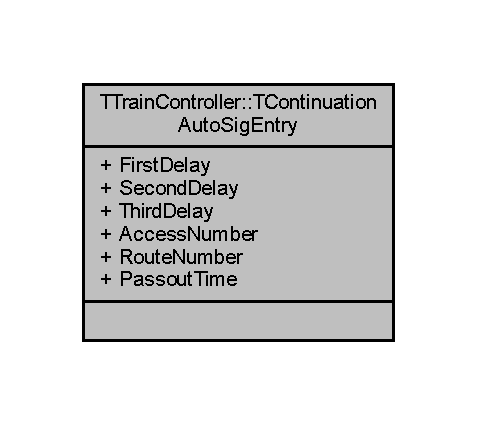
\includegraphics[width=229pt]{class_t_train_controller_1_1_t_continuation_auto_sig_entry__coll__graph}
\end{center}
\end{figure}
\subsection*{Public Attributes}
\begin{DoxyCompactItemize}
\item 
\mbox{\Hypertarget{class_t_train_controller_1_1_t_continuation_auto_sig_entry_ab5a944eed2be17d13d99a9070f78c785}\label{class_t_train_controller_1_1_t_continuation_auto_sig_entry_ab5a944eed2be17d13d99a9070f78c785}} 
double {\bfseries First\+Delay}
\item 
\mbox{\Hypertarget{class_t_train_controller_1_1_t_continuation_auto_sig_entry_a637042cd9aa1c141c68ca1979935c8d8}\label{class_t_train_controller_1_1_t_continuation_auto_sig_entry_a637042cd9aa1c141c68ca1979935c8d8}} 
double {\bfseries Second\+Delay}
\item 
\mbox{\Hypertarget{class_t_train_controller_1_1_t_continuation_auto_sig_entry_ad393d737f9031743cabfc1fbd1ac6239}\label{class_t_train_controller_1_1_t_continuation_auto_sig_entry_ad393d737f9031743cabfc1fbd1ac6239}} 
double {\bfseries Third\+Delay}
\item 
\mbox{\Hypertarget{class_t_train_controller_1_1_t_continuation_auto_sig_entry_ae4cf92f0e912fe54c7b9549ba4158e90}\label{class_t_train_controller_1_1_t_continuation_auto_sig_entry_ae4cf92f0e912fe54c7b9549ba4158e90}} 
int {\bfseries Access\+Number}
\item 
\mbox{\Hypertarget{class_t_train_controller_1_1_t_continuation_auto_sig_entry_a20f64023350c7394250f784b58a5c036}\label{class_t_train_controller_1_1_t_continuation_auto_sig_entry_a20f64023350c7394250f784b58a5c036}} 
int {\bfseries Route\+Number}
\item 
\mbox{\Hypertarget{class_t_train_controller_1_1_t_continuation_auto_sig_entry_a658b7d6efd311690bb9c36e3518e3ff5}\label{class_t_train_controller_1_1_t_continuation_auto_sig_entry_a658b7d6efd311690bb9c36e3518e3ff5}} 
T\+Date\+Time {\bfseries Passout\+Time}
\end{DoxyCompactItemize}


The documentation for this class was generated from the following file\+:\begin{DoxyCompactItemize}
\item 
Train\+Unit.\+h\end{DoxyCompactItemize}

\hypertarget{class_t_train_controller_1_1_t_continuation_train_expectation_entry}{}\section{T\+Train\+Controller\+:\+:T\+Continuation\+Train\+Expectation\+Entry Class Reference}
\label{class_t_train_controller_1_1_t_continuation_train_expectation_entry}\index{T\+Train\+Controller\+::\+T\+Continuation\+Train\+Expectation\+Entry@{T\+Train\+Controller\+::\+T\+Continuation\+Train\+Expectation\+Entry}}


Collaboration diagram for T\+Train\+Controller\+:\+:T\+Continuation\+Train\+Expectation\+Entry\+:\nopagebreak
\begin{figure}[H]
\begin{center}
\leavevmode
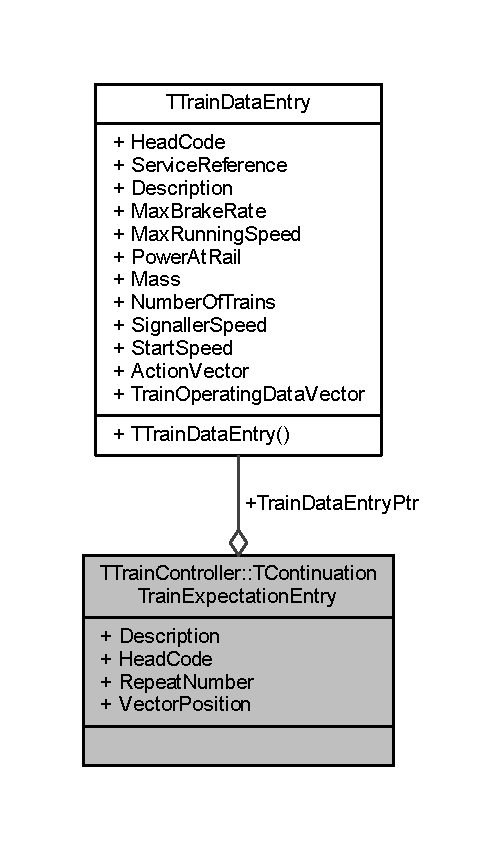
\includegraphics[width=242pt]{class_t_train_controller_1_1_t_continuation_train_expectation_entry__coll__graph}
\end{center}
\end{figure}
\subsection*{Public Attributes}
\begin{DoxyCompactItemize}
\item 
\mbox{\Hypertarget{class_t_train_controller_1_1_t_continuation_train_expectation_entry_a4f8cb6b7a1ab76fb56a56594aa440fe5}\label{class_t_train_controller_1_1_t_continuation_train_expectation_entry_a4f8cb6b7a1ab76fb56a56594aa440fe5}} 
Ansi\+String {\bfseries Description}
\item 
\mbox{\Hypertarget{class_t_train_controller_1_1_t_continuation_train_expectation_entry_a385c1cedb6c4c81c59f38bc2ef3c50d9}\label{class_t_train_controller_1_1_t_continuation_train_expectation_entry_a385c1cedb6c4c81c59f38bc2ef3c50d9}} 
Ansi\+String {\bfseries Head\+Code}
\item 
\mbox{\Hypertarget{class_t_train_controller_1_1_t_continuation_train_expectation_entry_aba462c168d94a8479f9b391b3ad90f5b}\label{class_t_train_controller_1_1_t_continuation_train_expectation_entry_aba462c168d94a8479f9b391b3ad90f5b}} 
int {\bfseries Repeat\+Number}
\item 
\mbox{\Hypertarget{class_t_train_controller_1_1_t_continuation_train_expectation_entry_a77f5a64b552a6d938b1ab2a0e3488c11}\label{class_t_train_controller_1_1_t_continuation_train_expectation_entry_a77f5a64b552a6d938b1ab2a0e3488c11}} 
int {\bfseries Vector\+Position}
\item 
\mbox{\Hypertarget{class_t_train_controller_1_1_t_continuation_train_expectation_entry_ad710cc4b0bde6c917aaba9c732773bcb}\label{class_t_train_controller_1_1_t_continuation_train_expectation_entry_ad710cc4b0bde6c917aaba9c732773bcb}} 
\mbox{\hyperlink{class_t_train_data_entry}{T\+Train\+Data\+Entry}} $\ast$ {\bfseries Train\+Data\+Entry\+Ptr}
\end{DoxyCompactItemize}


The documentation for this class was generated from the following file\+:\begin{DoxyCompactItemize}
\item 
Train\+Unit.\+h\end{DoxyCompactItemize}

\hypertarget{class_t_display}{}\section{T\+Display Class Reference}
\label{class_t_display}\index{T\+Display@{T\+Display}}


{\ttfamily \#include $<$Display\+Unit.\+h$>$}

\subsection*{Public Member Functions}
\begin{DoxyCompactItemize}
\item 
\mbox{\Hypertarget{class_t_display_aea01e701e8480ffa268b0de85782db80}\label{class_t_display_aea01e701e8480ffa268b0de85782db80}} 
Ansi\+String \mbox{\hyperlink{class_t_display_aea01e701e8480ffa268b0de85782db80}{Get\+Font\+Name}} ()
\begin{DoxyCompactList}\small\item\em Return the name of the default screen font. \end{DoxyCompactList}\item 
\mbox{\Hypertarget{class_t_display_a664e19dbba876f346496ad4c6d13c0a3}\label{class_t_display_a664e19dbba876f346496ad4c6d13c0a3}} 
int \mbox{\hyperlink{class_t_display_a664e19dbba876f346496ad4c6d13c0a3}{Get\+Font\+Size}} ()
\begin{DoxyCompactList}\small\item\em Return the size of the default screen font. \end{DoxyCompactList}\item 
\mbox{\Hypertarget{class_t_display_a5d3647a144c07e574430e7625e102ca9}\label{class_t_display_a5d3647a144c07e574430e7625e102ca9}} 
int \mbox{\hyperlink{class_t_display_a5d3647a144c07e574430e7625e102ca9}{Height}} ()
\begin{DoxyCompactList}\small\item\em Return the height of the screen. \end{DoxyCompactList}\item 
\mbox{\Hypertarget{class_t_display_a1b2004c2d76614da605291b06863f340}\label{class_t_display_a1b2004c2d76614da605291b06863f340}} 
int \mbox{\hyperlink{class_t_display_a1b2004c2d76614da605291b06863f340}{Left}} ()
\begin{DoxyCompactList}\small\item\em Return the left pixel position of the screen. \end{DoxyCompactList}\item 
\mbox{\Hypertarget{class_t_display_a7c843ab3083d7851ed199251d317f50a}\label{class_t_display_a7c843ab3083d7851ed199251d317f50a}} 
int \mbox{\hyperlink{class_t_display_a7c843ab3083d7851ed199251d317f50a}{Top}} ()
\begin{DoxyCompactList}\small\item\em Return the top pixel position of the screen. \end{DoxyCompactList}\item 
\mbox{\Hypertarget{class_t_display_a39cee11613d156de0d1f5df923a02c8d}\label{class_t_display_a39cee11613d156de0d1f5df923a02c8d}} 
int \mbox{\hyperlink{class_t_display_a39cee11613d156de0d1f5df923a02c8d}{Width}} ()
\begin{DoxyCompactList}\small\item\em Return the width of the screen. \end{DoxyCompactList}\item 
\mbox{\Hypertarget{class_t_display_a375ba345403e91af04392540fbd5f2f3}\label{class_t_display_a375ba345403e91af04392540fbd5f2f3}} 
T\+Font $\ast$ \mbox{\hyperlink{class_t_display_a375ba345403e91af04392540fbd5f2f3}{Get\+Font}} ()
\begin{DoxyCompactList}\small\item\em Return the current screen font. \end{DoxyCompactList}\item 
\mbox{\Hypertarget{class_t_display_a33f7067eea9e638bdc363bd0af70d7d5}\label{class_t_display_a33f7067eea9e638bdc363bd0af70d7d5}} 
T\+Image $\ast$ \mbox{\hyperlink{class_t_display_a33f7067eea9e638bdc363bd0af70d7d5}{Get\+Image}} ()
\begin{DoxyCompactList}\small\item\em Return a pointer to the screen image. \end{DoxyCompactList}\item 
\mbox{\Hypertarget{class_t_display_abaab175c40149d2a4c449e9463b21a42}\label{class_t_display_abaab175c40149d2a4c449e9463b21a42}} 
T\+Label $\ast$ \mbox{\hyperlink{class_t_display_abaab175c40149d2a4c449e9463b21a42}{Get\+Output\+Log1}} ()
\begin{DoxyCompactList}\small\item\em Return pointers to warning message logs (appear above the railway display during operation) \end{DoxyCompactList}\item 
\mbox{\Hypertarget{class_t_display_a913b1be885ac6fc291bf8367e0a8f6f0}\label{class_t_display_a913b1be885ac6fc291bf8367e0a8f6f0}} 
T\+Label $\ast$ {\bfseries Get\+Output\+Log2} ()
\item 
\mbox{\Hypertarget{class_t_display_a1e134169a934d995afa8fc6cb2d5dba3}\label{class_t_display_a1e134169a934d995afa8fc6cb2d5dba3}} 
T\+Label $\ast$ {\bfseries Get\+Output\+Log3} ()
\item 
\mbox{\Hypertarget{class_t_display_aba802332a11229140ce5871c0b6cc6f7}\label{class_t_display_aba802332a11229140ce5871c0b6cc6f7}} 
T\+Label $\ast$ {\bfseries Get\+Output\+Log4} ()
\item 
\mbox{\Hypertarget{class_t_display_a890f6524c617a499ddf6a33dedd402d5}\label{class_t_display_a890f6524c617a499ddf6a33dedd402d5}} 
T\+Label $\ast$ {\bfseries Get\+Output\+Log5} ()
\item 
\mbox{\Hypertarget{class_t_display_a6195645236a8467bb91251ebc05e7aaa}\label{class_t_display_a6195645236a8467bb91251ebc05e7aaa}} 
T\+Label $\ast$ {\bfseries Get\+Output\+Log6} ()
\item 
\mbox{\Hypertarget{class_t_display_abd6048be9875c6a05d5e03dafad392eb}\label{class_t_display_abd6048be9875c6a05d5e03dafad392eb}} 
T\+Label $\ast$ {\bfseries Get\+Output\+Log7} ()
\item 
\mbox{\Hypertarget{class_t_display_a6b64227ebcf1e3d89ab7b91935b34418}\label{class_t_display_a6b64227ebcf1e3d89ab7b91935b34418}} 
T\+Label $\ast$ {\bfseries Get\+Output\+Log8} ()
\item 
\mbox{\Hypertarget{class_t_display_a3c0d9e395bca910692d99bf290003a82}\label{class_t_display_a3c0d9e395bca910692d99bf290003a82}} 
T\+Label $\ast$ {\bfseries Get\+Output\+Log9} ()
\item 
\mbox{\Hypertarget{class_t_display_af3539f02f6a316b418aa5536cf52649c}\label{class_t_display_af3539f02f6a316b418aa5536cf52649c}} 
T\+Label $\ast$ {\bfseries Get\+Output\+Log10} ()
\item 
\mbox{\Hypertarget{class_t_display_abf4de4c2478e8e9d29316fa0e2b6cf8c}\label{class_t_display_abf4de4c2478e8e9d29316fa0e2b6cf8c}} 
void \mbox{\hyperlink{class_t_display_abf4de4c2478e8e9d29316fa0e2b6cf8c}{Cursor}} (T\+Cursor Cur)
\begin{DoxyCompactList}\small\item\em Set the screen cursor to \textquotesingle{}Cur\textquotesingle{} (used to select an arrow or an hourglass) \end{DoxyCompactList}\item 
\mbox{\Hypertarget{class_t_display_adc2d6f29794735d5fdebd7b2dbece95d}\label{class_t_display_adc2d6f29794735d5fdebd7b2dbece95d}} 
void \mbox{\hyperlink{class_t_display_adc2d6f29794735d5fdebd7b2dbece95d}{Reset\+Zoom\+In\+Offsets}} ()
\begin{DoxyCompactList}\small\item\em Reset the zoomed-\/in screen display to the \textquotesingle{}Home\textquotesingle{} position. \end{DoxyCompactList}\item 
\mbox{\Hypertarget{class_t_display_aae6570b04021b9a6e1748eb7f2bdf325}\label{class_t_display_aae6570b04021b9a6e1748eb7f2bdf325}} 
void \mbox{\hyperlink{class_t_display_aae6570b04021b9a6e1748eb7f2bdf325}{Reset\+Zoom\+Out\+Offsets}} ()
\begin{DoxyCompactList}\small\item\em Reset the zoomed-\/out screen display to the \textquotesingle{}Home\textquotesingle{} position. \end{DoxyCompactList}\item 
\mbox{\Hypertarget{class_t_display_af1ddcf928f3f5f3a39504f4e12bd51c0}\label{class_t_display_af1ddcf928f3f5f3a39504f4e12bd51c0}} 
void \mbox{\hyperlink{class_t_display_af1ddcf928f3f5f3a39504f4e12bd51c0}{Set\+Font}} (T\+Font $\ast$Font)
\begin{DoxyCompactList}\small\item\em Set the screen font to \textquotesingle{}Font\textquotesingle{}. \end{DoxyCompactList}\item 
\mbox{\Hypertarget{class_t_display_aa4f37ab2a4df6437a2219f303e1de40b}\label{class_t_display_aa4f37ab2a4df6437a2219f303e1de40b}} 
void \mbox{\hyperlink{class_t_display_aa4f37ab2a4df6437a2219f303e1de40b}{Update}} ()
\begin{DoxyCompactList}\small\item\em Repaint the screen display. \end{DoxyCompactList}\item 
\mbox{\hyperlink{class_t_display_a72cbdba53131a636da2c656f6025574b}{T\+Display}} (T\+Image $\ast$\&Image, T\+Memo $\ast$\&Memo\+Box, T\+Label $\ast$\&L1, T\+Label $\ast$\&L2, T\+Label $\ast$\&L3, T\+Label $\ast$\&L4, T\+Label $\ast$\&L5, T\+Label $\ast$\&L6, T\+Label $\ast$\&L7, T\+Label $\ast$\&L8, T\+Label $\ast$\&L9, T\+Label $\ast$\&L10)
\item 
\mbox{\Hypertarget{class_t_display_ab96c1fdec64997a8c252704ea6c231bf}\label{class_t_display_ab96c1fdec64997a8c252704ea6c231bf}} 
void \mbox{\hyperlink{class_t_display_ab96c1fdec64997a8c252704ea6c231bf}{Clear}} (int Caller, T\+Rect Rect)
\begin{DoxyCompactList}\small\item\em Empty the rectangle defined by Rect. \end{DoxyCompactList}\item 
\mbox{\Hypertarget{class_t_display_a8d990507ae0111e0b7890e8aa77fd76d}\label{class_t_display_a8d990507ae0111e0b7890e8aa77fd76d}} 
void \mbox{\hyperlink{class_t_display_a8d990507ae0111e0b7890e8aa77fd76d}{Clear\+Display}} (int Caller)
\begin{DoxyCompactList}\small\item\em Empty the display. \end{DoxyCompactList}\item 
\mbox{\Hypertarget{class_t_display_ac97de4f74b0b295de941320578d6da28}\label{class_t_display_ac97de4f74b0b295de941320578d6da28}} 
void \mbox{\hyperlink{class_t_display_ac97de4f74b0b295de941320578d6da28}{Ellipse}} (int Caller, int H\+Pos, int V\+Pos, T\+Color Col)
\begin{DoxyCompactList}\small\item\em Plot an ellipse at the defined position and with the defined colour. \end{DoxyCompactList}\item 
void \mbox{\hyperlink{class_t_display_a2b408bc588565f7b0cdcb85edc7479b7}{Get\+Rectangle}} (int Caller, T\+Rect Dest\+Rect, T\+Rect Source\+Rect, Graphics\+::\+T\+Bitmap $\ast$\&Original\+Graphic)
\item 
\mbox{\Hypertarget{class_t_display_ab77f8f220d8c0f3fbdcc96a616b969e6}\label{class_t_display_ab77f8f220d8c0f3fbdcc96a616b969e6}} 
void \mbox{\hyperlink{class_t_display_ab77f8f220d8c0f3fbdcc96a616b969e6}{Hide\+Warning\+Log}} (int Caller)
\begin{DoxyCompactList}\small\item\em Hide all the warnings from the top part of the screen -\/ for timetable clock adjustment. \end{DoxyCompactList}\item 
void \mbox{\hyperlink{class_t_display_a63930b93b9883463cd9d779e86fefba2}{Invert\+Element}} (int Caller, int H\+Pos, int V\+Pos)
\item 
\mbox{\Hypertarget{class_t_display_a92bea1eb27a17c6c7f902858d4115d71}\label{class_t_display_a92bea1eb27a17c6c7f902858d4115d71}} 
void \mbox{\hyperlink{class_t_display_a92bea1eb27a17c6c7f902858d4115d71}{Performance\+Log}} (int Caller, Ansi\+String Statement)
\begin{DoxyCompactList}\small\item\em Send Statement to the performance log on screen and to the file. \end{DoxyCompactList}\item 
void \mbox{\hyperlink{class_t_display_a7dae1c6470743a7cb778a6f813c7f0cc}{Plot\+Absolute}} (int Caller, int H\+Pos, int V\+Pos, Graphics\+::\+T\+Bitmap $\ast$Plot\+Item)
\item 
\mbox{\Hypertarget{class_t_display_ad601661fd4cd79a47b4c80ae77f901a9}\label{class_t_display_ad601661fd4cd79a47b4c80ae77f901a9}} 
void \mbox{\hyperlink{class_t_display_ad601661fd4cd79a47b4c80ae77f901a9}{Plot\+Blank}} (int Caller, int H\+Loc, int V\+Loc)
\begin{DoxyCompactList}\small\item\em Plot a blank track element at H\+Loc \& V\+Loc. \end{DoxyCompactList}\item 
\mbox{\Hypertarget{class_t_display_a09a60665a7a8c7b5d5c705a08086feec}\label{class_t_display_a09a60665a7a8c7b5d5c705a08086feec}} 
void \mbox{\hyperlink{class_t_display_a09a60665a7a8c7b5d5c705a08086feec}{Plot\+Dashed\+Rect}} (int Caller, T\+Rect Rect)
\begin{DoxyCompactList}\small\item\em Plot a dashed rectangle for the area defined by Rect, used when selecting display areas. \end{DoxyCompactList}\item 
\mbox{\Hypertarget{class_t_display_a9ab49e52c7eb92b32ae2c34547183439}\label{class_t_display_a9ab49e52c7eb92b32ae2c34547183439}} 
void \mbox{\hyperlink{class_t_display_a9ab49e52c7eb92b32ae2c34547183439}{Plot\+Output}} (int Caller, int H\+Pos, int V\+Pos, Graphics\+::\+T\+Bitmap $\ast$Plot\+Item)
\begin{DoxyCompactList}\small\item\em Plot the graphic at screen position H\+Pos \& V\+Pos. \end{DoxyCompactList}\item 
void \mbox{\hyperlink{class_t_display_aab35e517eba56f1c95f500958ce431ae}{Plot\+Point\+Blank}} (int Caller, int H\+Loc, int V\+Loc)
\item 
void \mbox{\hyperlink{class_t_display_a69c85bcbafea6cba5f06a93ffae7d3b2}{Plot\+Signal\+Blank}} (int Caller, int H\+Loc, int V\+Loc, int Speed\+Tag)
\item 
void \mbox{\hyperlink{class_t_display_ab6c0da6543f57f83107fd0af371fec3e}{Plot\+Signal\+Blank\+On\+Bitmap}} (int H\+Loc, int V\+Loc, int Speed\+Tag, Graphics\+::\+T\+Bitmap $\ast$Bitmap)
\item 
\mbox{\Hypertarget{class_t_display_a95aaa80515f0abb7715920b326b318dd}\label{class_t_display_a95aaa80515f0abb7715920b326b318dd}} 
void \mbox{\hyperlink{class_t_display_a95aaa80515f0abb7715920b326b318dd}{Plot\+Small\+Output}} (int Caller, int H\+Pos, int V\+Pos, Graphics\+::\+T\+Bitmap $\ast$Plot\+Item)
\begin{DoxyCompactList}\small\item\em Plot small (4x4) graphic Plot\+Item on the zoomed-\/out display at H\+Pos \& Vpos. \end{DoxyCompactList}\item 
\mbox{\Hypertarget{class_t_display_a9c7886bf1e4622e8560ad7558ede8dcc}\label{class_t_display_a9c7886bf1e4622e8560ad7558ede8dcc}} 
void \mbox{\hyperlink{class_t_display_a9c7886bf1e4622e8560ad7558ede8dcc}{Rectangle}} (int Caller, int H\+Pos, int V\+Pos, T\+Color Col, int Size, int \mbox{\hyperlink{class_t_display_a39cee11613d156de0d1f5df923a02c8d}{Width}})
\begin{DoxyCompactList}\small\item\em Plot a rectangle at the defined position with colour Col \& size defined by Size. \end{DoxyCompactList}\item 
\mbox{\Hypertarget{class_t_display_aece63da07b7586b62115eeb81c7e2b57}\label{class_t_display_aece63da07b7586b62115eeb81c7e2b57}} 
void \mbox{\hyperlink{class_t_display_aece63da07b7586b62115eeb81c7e2b57}{Show\+Warning\+Log}} (int Caller)
\begin{DoxyCompactList}\small\item\em Show the warnings after timetable clock adjusted. \end{DoxyCompactList}\item 
\mbox{\Hypertarget{class_t_display_adfff17bfef798b07b1e6bbfc6f5e0822}\label{class_t_display_adfff17bfef798b07b1e6bbfc6f5e0822}} 
void \mbox{\hyperlink{class_t_display_adfff17bfef798b07b1e6bbfc6f5e0822}{Text\+Out}} (int Caller, int H\+Pos, int V\+Pos, Ansi\+String Text\+String, T\+Font $\ast$Font)
\begin{DoxyCompactList}\small\item\em Display Text\+String at the defined position with the defined font. \end{DoxyCompactList}\item 
\mbox{\Hypertarget{class_t_display_a604d491a723df459bdcd54a4b9d1d9f2}\label{class_t_display_a604d491a723df459bdcd54a4b9d1d9f2}} 
void \mbox{\hyperlink{class_t_display_a604d491a723df459bdcd54a4b9d1d9f2}{Warning\+Log}} (int Caller, Ansi\+String Statement)
\begin{DoxyCompactList}\small\item\em Display warning message Statement in the bottom left hand warning position and scroll other messages up. \end{DoxyCompactList}\end{DoxyCompactItemize}
\subsection*{Public Attributes}
\begin{DoxyCompactItemize}
\item 
\mbox{\Hypertarget{class_t_display_a0ce29cc370b43313ff15bee9423bf338}\label{class_t_display_a0ce29cc370b43313ff15bee9423bf338}} 
bool \mbox{\hyperlink{class_t_display_a0ce29cc370b43313ff15bee9423bf338}{Zoom\+Out\+Flag}}
\begin{DoxyCompactList}\small\item\em true when zoomed-\/out \end{DoxyCompactList}\end{DoxyCompactItemize}
\subsection*{Static Public Attributes}
\begin{DoxyCompactItemize}
\item 
\mbox{\Hypertarget{class_t_display_a9a9f37c50df125f2543f251460caf841}\label{class_t_display_a9a9f37c50df125f2543f251460caf841}} 
static int \mbox{\hyperlink{class_t_display_a9a9f37c50df125f2543f251460caf841}{Display\+OffsetH}} = 0
\begin{DoxyCompactList}\small\item\em the horizontal offset of the displayed screen \end{DoxyCompactList}\item 
\mbox{\Hypertarget{class_t_display_a6f11e4ccff893eef6ab624a7430974c3}\label{class_t_display_a6f11e4ccff893eef6ab624a7430974c3}} 
static int \mbox{\hyperlink{class_t_display_a6f11e4ccff893eef6ab624a7430974c3}{Display\+OffsetV}} = 0
\begin{DoxyCompactList}\small\item\em the vertical offset of the displayed screen \end{DoxyCompactList}\item 
\mbox{\Hypertarget{class_t_display_aef050e7f3b440542a12bbccd27bcd99d}\label{class_t_display_aef050e7f3b440542a12bbccd27bcd99d}} 
static int \mbox{\hyperlink{class_t_display_aef050e7f3b440542a12bbccd27bcd99d}{Display\+Offset\+H\+Home}} = 0
\begin{DoxyCompactList}\small\item\em the horizontal offset of the \textquotesingle{}Home\textquotesingle{} display \end{DoxyCompactList}\item 
\mbox{\Hypertarget{class_t_display_a4ea243ff377fcc09d3da53dbb2b18dfe}\label{class_t_display_a4ea243ff377fcc09d3da53dbb2b18dfe}} 
static int \mbox{\hyperlink{class_t_display_a4ea243ff377fcc09d3da53dbb2b18dfe}{Display\+Offset\+V\+Home}} = 0
\begin{DoxyCompactList}\small\item\em the vertical offset of the \textquotesingle{}Home\textquotesingle{} display \end{DoxyCompactList}\item 
\mbox{\Hypertarget{class_t_display_aa26d2bf6d6d14ad1c853f81f06f25121}\label{class_t_display_aa26d2bf6d6d14ad1c853f81f06f25121}} 
static int \mbox{\hyperlink{class_t_display_aa26d2bf6d6d14ad1c853f81f06f25121}{Display\+Zoom\+Out\+OffsetH}} = 0
\begin{DoxyCompactList}\small\item\em the horizontal offset of the zoomed-\/out display \end{DoxyCompactList}\item 
\mbox{\Hypertarget{class_t_display_a3c63a18e8901299ab56176c034072b1c}\label{class_t_display_a3c63a18e8901299ab56176c034072b1c}} 
static int \mbox{\hyperlink{class_t_display_a3c63a18e8901299ab56176c034072b1c}{Display\+Zoom\+Out\+OffsetV}} = 0
\begin{DoxyCompactList}\small\item\em the verticalal offset of the zoomed-\/out display \end{DoxyCompactList}\item 
\mbox{\Hypertarget{class_t_display_a62c3d449d00b1a063a4bf7f212968e87}\label{class_t_display_a62c3d449d00b1a063a4bf7f212968e87}} 
static int \mbox{\hyperlink{class_t_display_a62c3d449d00b1a063a4bf7f212968e87}{Display\+Zoom\+Out\+Offset\+H\+Home}} = 0
\begin{DoxyCompactList}\small\item\em the horizontal offset of the zoomed-\/out \textquotesingle{}Home\textquotesingle{} display \end{DoxyCompactList}\item 
\mbox{\Hypertarget{class_t_display_a758f553cef2eb9b3eee4d491454a7da9}\label{class_t_display_a758f553cef2eb9b3eee4d491454a7da9}} 
static int \mbox{\hyperlink{class_t_display_a758f553cef2eb9b3eee4d491454a7da9}{Display\+Zoom\+Out\+Offset\+V\+Home}} = 0
\begin{DoxyCompactList}\small\item\em the vertical offset of the zoomed-\/out \textquotesingle{}Home\textquotesingle{} display \end{DoxyCompactList}\end{DoxyCompactItemize}
\subsection*{Private Attributes}
\begin{DoxyCompactItemize}
\item 
\mbox{\Hypertarget{class_t_display_a0e442bbdf413812064b3d0d200261cbc}\label{class_t_display_a0e442bbdf413812064b3d0d200261cbc}} 
T\+Image $\ast$\& \mbox{\hyperlink{class_t_display_a0e442bbdf413812064b3d0d200261cbc}{Output}}
\begin{DoxyCompactList}\small\item\em pointer to the 60 x 36 element railway display area \end{DoxyCompactList}\item 
\mbox{\Hypertarget{class_t_display_a62d6c2b2040a469fb6eb6177a8acc1f2}\label{class_t_display_a62d6c2b2040a469fb6eb6177a8acc1f2}} 
T\+Label $\ast$\& \mbox{\hyperlink{class_t_display_a62d6c2b2040a469fb6eb6177a8acc1f2}{Output\+Log1}}
\begin{DoxyCompactList}\small\item\em Pointers to the warning message logs (appear above the railway display during operation) \end{DoxyCompactList}\item 
\mbox{\Hypertarget{class_t_display_ad7a9ab1d203557810bdbfe39fad79855}\label{class_t_display_ad7a9ab1d203557810bdbfe39fad79855}} 
T\+Label $\ast$\& {\bfseries Output\+Log2}
\item 
\mbox{\Hypertarget{class_t_display_ae099b334095873971b46f5c4c5e0bd2e}\label{class_t_display_ae099b334095873971b46f5c4c5e0bd2e}} 
T\+Label $\ast$\& {\bfseries Output\+Log3}
\item 
\mbox{\Hypertarget{class_t_display_a4084cb29429480cfe74c86d84e376009}\label{class_t_display_a4084cb29429480cfe74c86d84e376009}} 
T\+Label $\ast$\& {\bfseries Output\+Log4}
\item 
\mbox{\Hypertarget{class_t_display_af5ac89214b13057a1bf2dae88b3dac96}\label{class_t_display_af5ac89214b13057a1bf2dae88b3dac96}} 
T\+Label $\ast$\& {\bfseries Output\+Log5}
\item 
\mbox{\Hypertarget{class_t_display_a3adf5d70fb01209e746cb3cd490294b4}\label{class_t_display_a3adf5d70fb01209e746cb3cd490294b4}} 
T\+Label $\ast$\& {\bfseries Output\+Log6}
\item 
\mbox{\Hypertarget{class_t_display_a1b134b87e594c2cd261210023fd11161}\label{class_t_display_a1b134b87e594c2cd261210023fd11161}} 
T\+Label $\ast$\& {\bfseries Output\+Log7}
\item 
\mbox{\Hypertarget{class_t_display_a9de95aeb0787e6c535cf6622b3a87d8d}\label{class_t_display_a9de95aeb0787e6c535cf6622b3a87d8d}} 
T\+Label $\ast$\& {\bfseries Output\+Log8}
\item 
\mbox{\Hypertarget{class_t_display_a5bf597b689a283f16b1aae5fe79ad2ec}\label{class_t_display_a5bf597b689a283f16b1aae5fe79ad2ec}} 
T\+Label $\ast$\& {\bfseries Output\+Log9}
\item 
\mbox{\Hypertarget{class_t_display_afc194f2bc9eda7fe8de600098c85d2ac}\label{class_t_display_afc194f2bc9eda7fe8de600098c85d2ac}} 
T\+Label $\ast$\& {\bfseries Output\+Log10}
\item 
\mbox{\Hypertarget{class_t_display_a4ecb842151b8cb4a56a72ec72b9ca682}\label{class_t_display_a4ecb842151b8cb4a56a72ec72b9ca682}} 
T\+Memo $\ast$\& \mbox{\hyperlink{class_t_display_a4ecb842151b8cb4a56a72ec72b9ca682}{Performance\+Memo}}
\begin{DoxyCompactList}\small\item\em pointer to the panel that displays the performance log \end{DoxyCompactList}\end{DoxyCompactItemize}


\subsection{Detailed Description}
Class that manages all aspects of the display

There are 2 objects -\/ Display, which is the screen, and Hidden\+Display, which is an internal object used when building a new display and transferred to Display when complete (avoids the flicker that would be visible if Display was built directly) 

\subsection{Constructor \& Destructor Documentation}
\mbox{\Hypertarget{class_t_display_a72cbdba53131a636da2c656f6025574b}\label{class_t_display_a72cbdba53131a636da2c656f6025574b}} 
\index{T\+Display@{T\+Display}!T\+Display@{T\+Display}}
\index{T\+Display@{T\+Display}!T\+Display@{T\+Display}}
\subsubsection{\texorpdfstring{T\+Display()}{TDisplay()}}
{\footnotesize\ttfamily T\+Display\+::\+T\+Display (\begin{DoxyParamCaption}\item[{T\+Image $\ast$\&}]{Image,  }\item[{T\+Memo $\ast$\&}]{Memo\+Box,  }\item[{T\+Label $\ast$\&}]{L1,  }\item[{T\+Label $\ast$\&}]{L2,  }\item[{T\+Label $\ast$\&}]{L3,  }\item[{T\+Label $\ast$\&}]{L4,  }\item[{T\+Label $\ast$\&}]{L5,  }\item[{T\+Label $\ast$\&}]{L6,  }\item[{T\+Label $\ast$\&}]{L7,  }\item[{T\+Label $\ast$\&}]{L8,  }\item[{T\+Label $\ast$\&}]{L9,  }\item[{T\+Label $\ast$\&}]{L10 }\end{DoxyParamCaption})}

Constructor, sets the screen image (Main\+Screen or Hidden\+Screen), the performance log panel and the warning message labels 

\subsection{Member Function Documentation}
\mbox{\Hypertarget{class_t_display_a2b408bc588565f7b0cdcb85edc7479b7}\label{class_t_display_a2b408bc588565f7b0cdcb85edc7479b7}} 
\index{T\+Display@{T\+Display}!Get\+Rectangle@{Get\+Rectangle}}
\index{Get\+Rectangle@{Get\+Rectangle}!T\+Display@{T\+Display}}
\subsubsection{\texorpdfstring{Get\+Rectangle()}{GetRectangle()}}
{\footnotesize\ttfamily void T\+Display\+::\+Get\+Rectangle (\begin{DoxyParamCaption}\item[{int}]{Caller,  }\item[{T\+Rect}]{Dest\+Rect,  }\item[{T\+Rect}]{Source\+Rect,  }\item[{Graphics\+::\+T\+Bitmap $\ast$\&}]{Original\+Graphic }\end{DoxyParamCaption})}

Used in \mbox{\hyperlink{class_t_graphic_element_ac12f60cb52eefdc86eaa504419eb138d}{T\+Graphic\+Element\+::\+Load\+Original\+Screen\+Graphic}} in Track\+Unit to obtain Original\+Graphic from an area of the screen defined by Source\+Rect \mbox{\Hypertarget{class_t_display_a63930b93b9883463cd9d779e86fefba2}\label{class_t_display_a63930b93b9883463cd9d779e86fefba2}} 
\index{T\+Display@{T\+Display}!Invert\+Element@{Invert\+Element}}
\index{Invert\+Element@{Invert\+Element}!T\+Display@{T\+Display}}
\subsubsection{\texorpdfstring{Invert\+Element()}{InvertElement()}}
{\footnotesize\ttfamily void T\+Display\+::\+Invert\+Element (\begin{DoxyParamCaption}\item[{int}]{Caller,  }\item[{int}]{H\+Pos,  }\item[{int}]{V\+Pos }\end{DoxyParamCaption})}

Display the track element at H\+Pos \& V\+Pos inverted (used to show an offending element when trying to connect track \mbox{\Hypertarget{class_t_display_a7dae1c6470743a7cb778a6f813c7f0cc}\label{class_t_display_a7dae1c6470743a7cb778a6f813c7f0cc}} 
\index{T\+Display@{T\+Display}!Plot\+Absolute@{Plot\+Absolute}}
\index{Plot\+Absolute@{Plot\+Absolute}!T\+Display@{T\+Display}}
\subsubsection{\texorpdfstring{Plot\+Absolute()}{PlotAbsolute()}}
{\footnotesize\ttfamily void T\+Display\+::\+Plot\+Absolute (\begin{DoxyParamCaption}\item[{int}]{Caller,  }\item[{int}]{H\+Pos,  }\item[{int}]{V\+Pos,  }\item[{Graphics\+::\+T\+Bitmap $\ast$}]{Plot\+Item }\end{DoxyParamCaption})}

Plot the graphic at the railway (not screen) position set by H\+Pos \& V\+Pos \mbox{\Hypertarget{class_t_display_aab35e517eba56f1c95f500958ce431ae}\label{class_t_display_aab35e517eba56f1c95f500958ce431ae}} 
\index{T\+Display@{T\+Display}!Plot\+Point\+Blank@{Plot\+Point\+Blank}}
\index{Plot\+Point\+Blank@{Plot\+Point\+Blank}!T\+Display@{T\+Display}}
\subsubsection{\texorpdfstring{Plot\+Point\+Blank()}{PlotPointBlank()}}
{\footnotesize\ttfamily void T\+Display\+::\+Plot\+Point\+Blank (\begin{DoxyParamCaption}\item[{int}]{Caller,  }\item[{int}]{H\+Loc,  }\item[{int}]{V\+Loc }\end{DoxyParamCaption})}

Plot a small blank rectangle in the centre of a set of points at H\+Loc \& V\+Loc prior to plotting one or both fillets (the movable section) \mbox{\Hypertarget{class_t_display_a69c85bcbafea6cba5f06a93ffae7d3b2}\label{class_t_display_a69c85bcbafea6cba5f06a93ffae7d3b2}} 
\index{T\+Display@{T\+Display}!Plot\+Signal\+Blank@{Plot\+Signal\+Blank}}
\index{Plot\+Signal\+Blank@{Plot\+Signal\+Blank}!T\+Display@{T\+Display}}
\subsubsection{\texorpdfstring{Plot\+Signal\+Blank()}{PlotSignalBlank()}}
{\footnotesize\ttfamily void T\+Display\+::\+Plot\+Signal\+Blank (\begin{DoxyParamCaption}\item[{int}]{Caller,  }\item[{int}]{H\+Loc,  }\item[{int}]{V\+Loc,  }\item[{int}]{Speed\+Tag }\end{DoxyParamCaption})}

Plot a small blank rectangle over the signal aspect area at H\+Loc \& V\+Loc prior to plotting the current signal aspect \mbox{\Hypertarget{class_t_display_ab6c0da6543f57f83107fd0af371fec3e}\label{class_t_display_ab6c0da6543f57f83107fd0af371fec3e}} 
\index{T\+Display@{T\+Display}!Plot\+Signal\+Blank\+On\+Bitmap@{Plot\+Signal\+Blank\+On\+Bitmap}}
\index{Plot\+Signal\+Blank\+On\+Bitmap@{Plot\+Signal\+Blank\+On\+Bitmap}!T\+Display@{T\+Display}}
\subsubsection{\texorpdfstring{Plot\+Signal\+Blank\+On\+Bitmap()}{PlotSignalBlankOnBitmap()}}
{\footnotesize\ttfamily void T\+Display\+::\+Plot\+Signal\+Blank\+On\+Bitmap (\begin{DoxyParamCaption}\item[{int}]{H\+Loc,  }\item[{int}]{V\+Loc,  }\item[{int}]{Speed\+Tag,  }\item[{Graphics\+::\+T\+Bitmap $\ast$}]{Bitmap }\end{DoxyParamCaption})}

As Plot\+Signal\+Blank but plot on the Bitmap that is supplied
\begin{DoxyItemize}
\item for writing operating images to a bitmap file 
\end{DoxyItemize}

The documentation for this class was generated from the following files\+:\begin{DoxyCompactItemize}
\item 
Display\+Unit.\+h\item 
Display\+Unit.\+cpp\end{DoxyCompactItemize}

\hypertarget{class_t_fixed_track_piece}{}\section{T\+Fixed\+Track\+Piece Class Reference}
\label{class_t_fixed_track_piece}\index{T\+Fixed\+Track\+Piece@{T\+Fixed\+Track\+Piece}}


All basic track building blocks \& methods.  




{\ttfamily \#include $<$Track\+Unit.\+h$>$}

Inheritance diagram for T\+Fixed\+Track\+Piece\+:\begin{figure}[H]
\begin{center}
\leavevmode
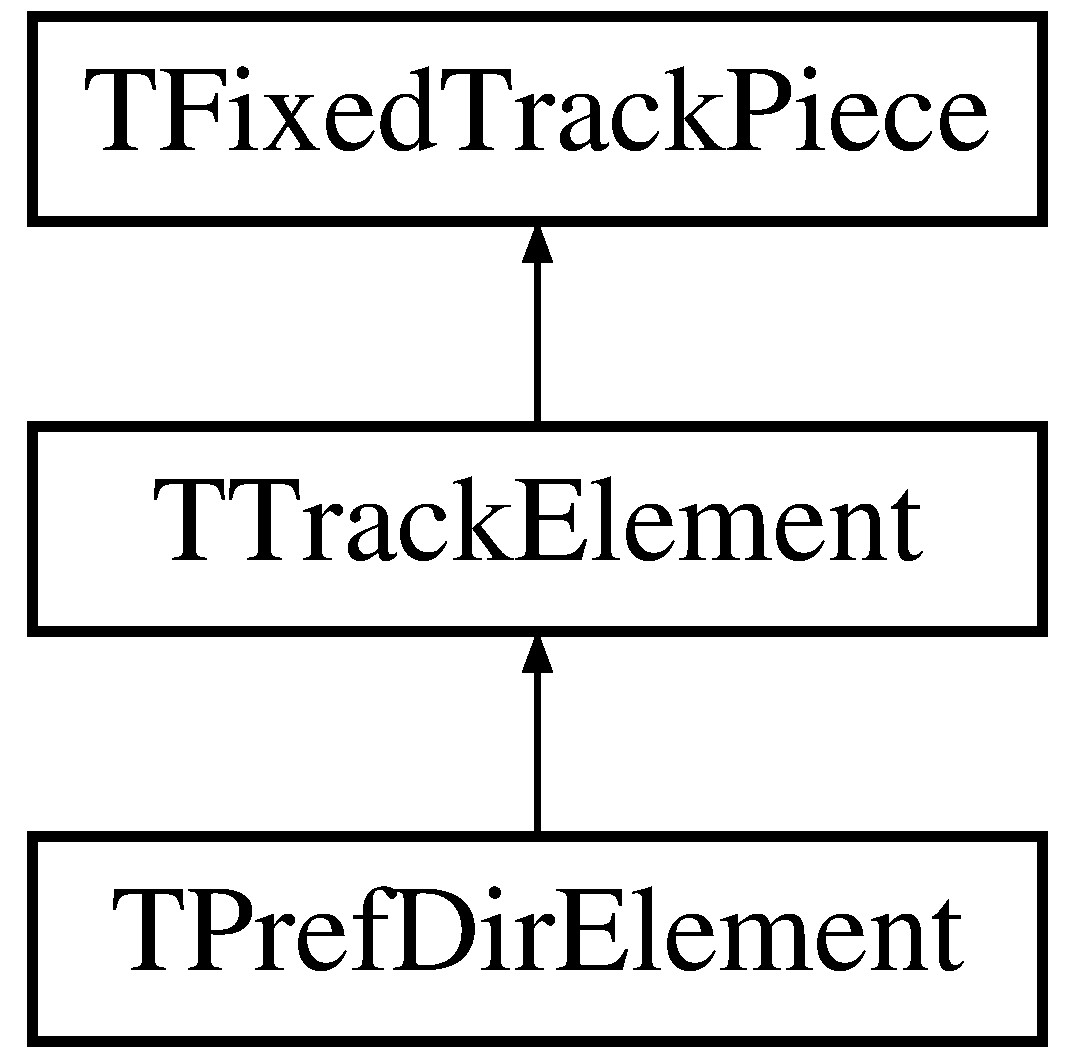
\includegraphics[height=3.000000cm]{class_t_fixed_track_piece}
\end{center}
\end{figure}
\subsection*{Public Member Functions}
\begin{DoxyCompactItemize}
\item 
\mbox{\Hypertarget{class_t_fixed_track_piece_a13eca615770d45f35bb808eaa264fda9}\label{class_t_fixed_track_piece_a13eca615770d45f35bb808eaa264fda9}} 
void \mbox{\hyperlink{class_t_fixed_track_piece_a13eca615770d45f35bb808eaa264fda9}{Plot\+Fixed\+Track\+Element}} (int Caller, int H\+Loc\+Input, int V\+Loc\+Input) const
\begin{DoxyCompactList}\small\item\em Plot the element on the railway display at position H\+Loc\+Input \& V\+Loc\+Input. \end{DoxyCompactList}\item 
\mbox{\Hypertarget{class_t_fixed_track_piece_af9d54643faf473becbc953a11eacab51}\label{class_t_fixed_track_piece_af9d54643faf473becbc953a11eacab51}} 
\mbox{\hyperlink{class_t_fixed_track_piece_af9d54643faf473becbc953a11eacab51}{T\+Fixed\+Track\+Piece}} (int Speed\+Tag\+Val, T\+Track\+Type Track\+Type\+Val, int Lk\+Val\mbox{[}4\mbox{]}, T\+Configuration Config\+Val\mbox{[}4\mbox{]}, Graphics\+::\+T\+Bitmap $\ast$Graphic\+Ptr\+Val, Graphics\+::\+T\+Bitmap $\ast$Small\+Graphic\+Ptr\+Val)
\begin{DoxyCompactList}\small\item\em Constructor for building T\+Track.\+Fixed\+Track\+Array -\/ see below. \end{DoxyCompactList}\item 
\mbox{\Hypertarget{class_t_fixed_track_piece_a5b7733fb7da20c74bd811743d70cd535}\label{class_t_fixed_track_piece_a5b7733fb7da20c74bd811743d70cd535}} 
\mbox{\hyperlink{class_t_fixed_track_piece_a5b7733fb7da20c74bd811743d70cd535}{T\+Fixed\+Track\+Piece}} ()
\begin{DoxyCompactList}\small\item\em Default constructor. \end{DoxyCompactList}\end{DoxyCompactItemize}
\subsection*{Public Attributes}
\begin{DoxyCompactItemize}
\item 
bool \mbox{\hyperlink{class_t_fixed_track_piece_a2d225bf10a7fb1c7e8ffd924b4d4ed2a}{Fixed\+Named\+Location\+Element}}
\item 
\mbox{\Hypertarget{class_t_fixed_track_piece_ad4f1d13f7b7c0dc13ad378706aa55238}\label{class_t_fixed_track_piece_ad4f1d13f7b7c0dc13ad378706aa55238}} 
int \mbox{\hyperlink{class_t_fixed_track_piece_ad4f1d13f7b7c0dc13ad378706aa55238}{Speed\+Tag}}
\begin{DoxyCompactList}\small\item\em The element identification number -\/ corresponds to the relevant Speed\+Button-\/$>$Tag. \end{DoxyCompactList}\item 
int \mbox{\hyperlink{class_t_fixed_track_piece_a6f604279e2311669576eb9bf36d8cfee}{Link}} \mbox{[}4\mbox{]}
\item 
\mbox{\Hypertarget{class_t_fixed_track_piece_a2a8cecb1cf81e95b1ee665dedc4c2465}\label{class_t_fixed_track_piece_a2a8cecb1cf81e95b1ee665dedc4c2465}} 
Graphics\+::\+T\+Bitmap $\ast$ \mbox{\hyperlink{class_t_fixed_track_piece_a2a8cecb1cf81e95b1ee665dedc4c2465}{Graphic\+Ptr}}
\begin{DoxyCompactList}\small\item\em the track bitmap for display on the zoomed-\/in railway \end{DoxyCompactList}\item 
\mbox{\Hypertarget{class_t_fixed_track_piece_a17923e22e532556ac072acaec3931621}\label{class_t_fixed_track_piece_a17923e22e532556ac072acaec3931621}} 
Graphics\+::\+T\+Bitmap $\ast$ \mbox{\hyperlink{class_t_fixed_track_piece_a17923e22e532556ac072acaec3931621}{Small\+Graphic\+Ptr}}
\begin{DoxyCompactList}\small\item\em the track bitmap for display on the zoomed-\/out railway \end{DoxyCompactList}\item 
\mbox{\Hypertarget{class_t_fixed_track_piece_ab0230b6fb2112bce31f205ae7ed5fd07}\label{class_t_fixed_track_piece_ab0230b6fb2112bce31f205ae7ed5fd07}} 
T\+Configuration \mbox{\hyperlink{class_t_fixed_track_piece_ab0230b6fb2112bce31f205ae7ed5fd07}{Config}} \mbox{[}4\mbox{]}
\begin{DoxyCompactList}\small\item\em the type of link -\/ see T\+Configuration above \end{DoxyCompactList}\item 
\mbox{\Hypertarget{class_t_fixed_track_piece_ad6c717a22333f52d1158dc57319e9e2a}\label{class_t_fixed_track_piece_ad6c717a22333f52d1158dc57319e9e2a}} 
T\+Track\+Type \mbox{\hyperlink{class_t_fixed_track_piece_ad6c717a22333f52d1158dc57319e9e2a}{Track\+Type}}
\begin{DoxyCompactList}\small\item\em the type of track element \end{DoxyCompactList}\end{DoxyCompactItemize}


\subsection{Detailed Description}
All basic track building blocks \& methods. 

\subsection{Member Data Documentation}
\mbox{\Hypertarget{class_t_fixed_track_piece_a2d225bf10a7fb1c7e8ffd924b4d4ed2a}\label{class_t_fixed_track_piece_a2d225bf10a7fb1c7e8ffd924b4d4ed2a}} 
\index{T\+Fixed\+Track\+Piece@{T\+Fixed\+Track\+Piece}!Fixed\+Named\+Location\+Element@{Fixed\+Named\+Location\+Element}}
\index{Fixed\+Named\+Location\+Element@{Fixed\+Named\+Location\+Element}!T\+Fixed\+Track\+Piece@{T\+Fixed\+Track\+Piece}}
\subsubsection{\texorpdfstring{Fixed\+Named\+Location\+Element}{FixedNamedLocationElement}}
{\footnotesize\ttfamily bool T\+Fixed\+Track\+Piece\+::\+Fixed\+Named\+Location\+Element}

true for an element that can be named (platforms, concourse, footbridges \& non-\/station named loactions) \mbox{\Hypertarget{class_t_fixed_track_piece_a6f604279e2311669576eb9bf36d8cfee}\label{class_t_fixed_track_piece_a6f604279e2311669576eb9bf36d8cfee}} 
\index{T\+Fixed\+Track\+Piece@{T\+Fixed\+Track\+Piece}!Link@{Link}}
\index{Link@{Link}!T\+Fixed\+Track\+Piece@{T\+Fixed\+Track\+Piece}}
\subsubsection{\texorpdfstring{Link}{Link}}
{\footnotesize\ttfamily int T\+Fixed\+Track\+Piece\+::\+Link\mbox{[}4\mbox{]}}

Track connection link values, max. of 4, unused = -\/1, top lh diag.=1, top=2, top rh diag.=3 left=4, right=6, bottom lh diag.=7, bottom=8, bottom rh diag.=9 

The documentation for this class was generated from the following files\+:\begin{DoxyCompactItemize}
\item 
C\+:/\+Programming work/railway development after v2.\+2.\+0/Track\+Unit.\+h\item 
C\+:/\+Programming work/railway development after v2.\+2.\+0/Track\+Unit.\+cpp\end{DoxyCompactItemize}

\hypertarget{class_t_graphic_element}{}\section{T\+Graphic\+Element Class Reference}
\label{class_t_graphic_element}\index{T\+Graphic\+Element@{T\+Graphic\+Element}}


{\ttfamily \#include $<$Track\+Unit.\+h$>$}

\subsection*{Public Member Functions}
\begin{DoxyCompactItemize}
\item 
\mbox{\Hypertarget{class_t_graphic_element_aaf109e208515c9b9aaad753d829d25e9}\label{class_t_graphic_element_aaf109e208515c9b9aaad753d829d25e9}} 
int {\bfseries Get\+H\+Pos} ()
\item 
\mbox{\Hypertarget{class_t_graphic_element_ad2780e85ae1e401bfbb6a7c37b15bea8}\label{class_t_graphic_element_ad2780e85ae1e401bfbb6a7c37b15bea8}} 
int {\bfseries Get\+V\+Pos} ()
\item 
void \mbox{\hyperlink{class_t_graphic_element_adffdc9f9c4a5fff5cbeab6b5a027dad9}{Set\+Source\+Rect}} (int Left, int Top)
\item 
\mbox{\Hypertarget{class_t_graphic_element_a6c3759e5c5a639ef98c3470363c48988}\label{class_t_graphic_element_a6c3759e5c5a639ef98c3470363c48988}} 
void \mbox{\hyperlink{class_t_graphic_element_a6c3759e5c5a639ef98c3470363c48988}{Load\+Original\+Existing\+Graphic}} (int Caller, int H\+Offset, int V\+Offset, int Width\+In, int Height\+In, Graphics\+::\+T\+Bitmap $\ast$Graphic)
\begin{DoxyCompactList}\small\item\em Load red or green gap flashing graphic from the stored bitmaps. \end{DoxyCompactList}\item 
\mbox{\Hypertarget{class_t_graphic_element_ac12f60cb52eefdc86eaa504419eb138d}\label{class_t_graphic_element_ac12f60cb52eefdc86eaa504419eb138d}} 
void \mbox{\hyperlink{class_t_graphic_element_ac12f60cb52eefdc86eaa504419eb138d}{Load\+Original\+Screen\+Graphic}} (int Caller)
\begin{DoxyCompactList}\small\item\em Load original graphic from the screen for point flashing or route start markers. \end{DoxyCompactList}\item 
\mbox{\Hypertarget{class_t_graphic_element_a82c786873b196ec443f052dedac8b1c1}\label{class_t_graphic_element_a82c786873b196ec443f052dedac8b1c1}} 
void \mbox{\hyperlink{class_t_graphic_element_a82c786873b196ec443f052dedac8b1c1}{Load\+Overlay\+Graphic}} (int Caller, Graphics\+::\+T\+Bitmap $\ast$Overlay)
\begin{DoxyCompactList}\small\item\em Load the temporary overlay graphic. \end{DoxyCompactList}\item 
\mbox{\Hypertarget{class_t_graphic_element_a04ccc26451ff7d95dc3c5951b71f421e}\label{class_t_graphic_element_a04ccc26451ff7d95dc3c5951b71f421e}} 
void \mbox{\hyperlink{class_t_graphic_element_a04ccc26451ff7d95dc3c5951b71f421e}{Plot\+Overlay}} (int Caller, \mbox{\hyperlink{class_t_display}{T\+Display}} $\ast$Disp)
\begin{DoxyCompactList}\small\item\em Plot the overlay graphic on screen. \end{DoxyCompactList}\item 
\mbox{\Hypertarget{class_t_graphic_element_ad9e23ba031b1110126227d301b59ffc7}\label{class_t_graphic_element_ad9e23ba031b1110126227d301b59ffc7}} 
void \mbox{\hyperlink{class_t_graphic_element_ad9e23ba031b1110126227d301b59ffc7}{Plot\+Original}} (int Caller, \mbox{\hyperlink{class_t_display}{T\+Display}} $\ast$Disp)
\begin{DoxyCompactList}\small\item\em Plot the original graphic on screen. \end{DoxyCompactList}\item 
\mbox{\Hypertarget{class_t_graphic_element_afbfce56e5041fa0ac49b3ba49f7566fd}\label{class_t_graphic_element_afbfce56e5041fa0ac49b3ba49f7566fd}} 
void \mbox{\hyperlink{class_t_graphic_element_afbfce56e5041fa0ac49b3ba49f7566fd}{Set\+Screen\+H\+V\+Source}} (int Caller, int H\+Pos\+In, int V\+Pos\+In)
\begin{DoxyCompactList}\small\item\em Set H\+Pos, V\+Pos \& Source\+Rect member values from the supplied positions. \end{DoxyCompactList}\item 
\mbox{\Hypertarget{class_t_graphic_element_a037be3b14fb32ebac36bbee7b76a6fc1}\label{class_t_graphic_element_a037be3b14fb32ebac36bbee7b76a6fc1}} 
\mbox{\hyperlink{class_t_graphic_element_a037be3b14fb32ebac36bbee7b76a6fc1}{T\+Graphic\+Element}} ()
\begin{DoxyCompactList}\small\item\em Default constructor (16 x 16 pixel element) \end{DoxyCompactList}\item 
\mbox{\Hypertarget{class_t_graphic_element_a3d9336aecdb5c05c0d96485d896c8d24}\label{class_t_graphic_element_a3d9336aecdb5c05c0d96485d896c8d24}} 
\mbox{\hyperlink{class_t_graphic_element_a3d9336aecdb5c05c0d96485d896c8d24}{T\+Graphic\+Element}} (int Width\+In, int Height\+In)
\begin{DoxyCompactList}\small\item\em Constructor for specified dimensions. \end{DoxyCompactList}\item 
\mbox{\Hypertarget{class_t_graphic_element_af7a475400bc15a5ab41bf1b3d345dc31}\label{class_t_graphic_element_af7a475400bc15a5ab41bf1b3d345dc31}} 
\mbox{\hyperlink{class_t_graphic_element_af7a475400bc15a5ab41bf1b3d345dc31}{$\sim$\+T\+Graphic\+Element}} ()
\begin{DoxyCompactList}\small\item\em Destructor. \end{DoxyCompactList}\end{DoxyCompactItemize}
\subsection*{Private Attributes}
\begin{DoxyCompactItemize}
\item 
\mbox{\Hypertarget{class_t_graphic_element_a346a9ac23010defeaec2ba5e3b15e2fb}\label{class_t_graphic_element_a346a9ac23010defeaec2ba5e3b15e2fb}} 
bool {\bfseries Overlay\+Plotted}
\item 
\mbox{\Hypertarget{class_t_graphic_element_a8a4d5766d6ba3419beaab94bac20da89}\label{class_t_graphic_element_a8a4d5766d6ba3419beaab94bac20da89}} 
bool {\bfseries Overlay\+Loaded}
\item 
\mbox{\Hypertarget{class_t_graphic_element_abc32d53fda4618426c9acc8614cad7ef}\label{class_t_graphic_element_abc32d53fda4618426c9acc8614cad7ef}} 
bool {\bfseries Original\+Loaded}
\item 
\mbox{\Hypertarget{class_t_graphic_element_a63c8c1a8ad01f515e0c906dd48e6675e}\label{class_t_graphic_element_a63c8c1a8ad01f515e0c906dd48e6675e}} 
bool {\bfseries Screen\+Source\+Set}
\item 
\mbox{\Hypertarget{class_t_graphic_element_a9e9bb81c5f42be1f760c905f3697701e}\label{class_t_graphic_element_a9e9bb81c5f42be1f760c905f3697701e}} 
bool {\bfseries Screen\+Graphic\+Loaded}
\item 
\mbox{\Hypertarget{class_t_graphic_element_a751ff95653c3c7c70299c51657bd2195}\label{class_t_graphic_element_a751ff95653c3c7c70299c51657bd2195}} 
bool \mbox{\hyperlink{class_t_graphic_element_a751ff95653c3c7c70299c51657bd2195}{Existing\+Graphic\+Loaded}}
\begin{DoxyCompactList}\small\item\em state flags \end{DoxyCompactList}\item 
\mbox{\Hypertarget{class_t_graphic_element_abc0d517132a89b44f93d599aa3528030}\label{class_t_graphic_element_abc0d517132a89b44f93d599aa3528030}} 
int {\bfseries H\+Pos}
\item 
\mbox{\Hypertarget{class_t_graphic_element_a5f06e91844e62b9975b6128921746178}\label{class_t_graphic_element_a5f06e91844e62b9975b6128921746178}} 
int \mbox{\hyperlink{class_t_graphic_element_a5f06e91844e62b9975b6128921746178}{V\+Pos}}
\begin{DoxyCompactList}\small\item\em horizontal and vertical positions \end{DoxyCompactList}\item 
\mbox{\Hypertarget{class_t_graphic_element_a5449d46461dbf9108441020cdd00c0ae}\label{class_t_graphic_element_a5449d46461dbf9108441020cdd00c0ae}} 
int {\bfseries Width}
\item 
\mbox{\Hypertarget{class_t_graphic_element_aa7e2feb822e3a00228b582e0c8b6d277}\label{class_t_graphic_element_aa7e2feb822e3a00228b582e0c8b6d277}} 
int \mbox{\hyperlink{class_t_graphic_element_aa7e2feb822e3a00228b582e0c8b6d277}{Height}}
\begin{DoxyCompactList}\small\item\em dimensions in pixels \end{DoxyCompactList}\item 
\mbox{\Hypertarget{class_t_graphic_element_a5de04c4143742c4247e4015dc7554fad}\label{class_t_graphic_element_a5de04c4143742c4247e4015dc7554fad}} 
Graphics\+::\+T\+Bitmap $\ast$ {\bfseries Original\+Graphic}
\item 
\mbox{\Hypertarget{class_t_graphic_element_a129fc709d76f28924aa71d2f8ba1ecc7}\label{class_t_graphic_element_a129fc709d76f28924aa71d2f8ba1ecc7}} 
Graphics\+::\+T\+Bitmap $\ast$ \mbox{\hyperlink{class_t_graphic_element_a129fc709d76f28924aa71d2f8ba1ecc7}{Overlay\+Graphic}}
\begin{DoxyCompactList}\small\item\em original and temporary overlay graphics \end{DoxyCompactList}\item 
\mbox{\Hypertarget{class_t_graphic_element_af4a75f077eac76c1f14c66571ff2f3b3}\label{class_t_graphic_element_af4a75f077eac76c1f14c66571ff2f3b3}} 
T\+Rect \mbox{\hyperlink{class_t_graphic_element_af4a75f077eac76c1f14c66571ff2f3b3}{Source\+Rect}}
\begin{DoxyCompactList}\small\item\em source rectangle of the original graphic \end{DoxyCompactList}\end{DoxyCompactItemize}


\subsection{Detailed Description}
Allows a single Width x Height graphic to change and change back independently of the remaining display

Used for the flashing green and red gap markers, flashing points and route start graphics. The code is mostly self-\/explanatory, but Set\+Screen\+H\+V\+Source (sets source rectangle) must be called before the original graphic is loaded, whether or not the graphic is loaded from the screen (using Load\+Original\+Screen\+Graphic, for point flashing and route start markers) or an existing bitmap (using Load\+Original\+Existing\+Graphic, for red and green gap flashing), and Overlay\+Graphic and Original\+Graphic must be loaded before they are plotted. Checks are built in for these conditions. Source\+Rect is the rectangle on the appropriate canvas where the original graphic is taken from. The original graphic can be taken from the screen -\/ \mbox{\hyperlink{class_t_graphic_element_ac12f60cb52eefdc86eaa504419eb138d}{Load\+Original\+Screen\+Graphic()}}, or from a section from an existing bitmap -\/ Load\+Original\+Existing\+Graphic. If an existing bitmap is selected then the loading function overrides the size that was set in the constructor, and Source\+Rect \& H\+Pos \& V\+Pos that were set in Set\+Screen\+H\+V\+Source. 

\subsection{Member Function Documentation}
\mbox{\Hypertarget{class_t_graphic_element_adffdc9f9c4a5fff5cbeab6b5a027dad9}\label{class_t_graphic_element_adffdc9f9c4a5fff5cbeab6b5a027dad9}} 
\index{T\+Graphic\+Element@{T\+Graphic\+Element}!Set\+Source\+Rect@{Set\+Source\+Rect}}
\index{Set\+Source\+Rect@{Set\+Source\+Rect}!T\+Graphic\+Element@{T\+Graphic\+Element}}
\subsubsection{\texorpdfstring{Set\+Source\+Rect()}{SetSourceRect()}}
{\footnotesize\ttfamily void T\+Graphic\+Element\+::\+Set\+Source\+Rect (\begin{DoxyParamCaption}\item[{int}]{Left,  }\item[{int}]{Top }\end{DoxyParamCaption})\hspace{0.3cm}{\ttfamily [inline]}}

Set Source\+Rect member values from those supplied and existing Width \& Height


\begin{DoxyItemize}
\item ensure this is only called after Width \& Height are set 
\end{DoxyItemize}

The documentation for this class was generated from the following files\+:\begin{DoxyCompactItemize}
\item 
Track\+Unit.\+h\item 
Track\+Unit.\+cpp\end{DoxyCompactItemize}

\hypertarget{class_t_interface}{}\section{T\+Interface Class Reference}
\label{class_t_interface}\index{T\+Interface@{T\+Interface}}


Inheritance diagram for T\+Interface\+:
\nopagebreak
\begin{figure}[H]
\begin{center}
\leavevmode
\includegraphics[height=550pt]{class_t_interface__inherit__graph}
\end{center}
\end{figure}


Collaboration diagram for T\+Interface\+:
\nopagebreak
\begin{figure}[H]
\begin{center}
\leavevmode
\includegraphics[height=550pt]{class_t_interface__coll__graph}
\end{center}
\end{figure}
\subsection*{Public Types}
\begin{DoxyCompactItemize}
\item 
\mbox{\Hypertarget{class_t_interface_afdd8ad9ea5529b9193c4b4c5ac683bc5}\label{class_t_interface_afdd8ad9ea5529b9193c4b4c5ac683bc5}} 
enum {\bfseries T\+Level1\+Mode} \{ \newline
{\bfseries Base\+Mode}, 
{\bfseries Track\+Mode}, 
{\bfseries Pref\+Dir\+Mode}, 
{\bfseries Oper\+Mode}, 
\newline
{\bfseries Restart\+Session\+Oper\+Mode}, 
{\bfseries Timetable\+Mode}
 \}
\end{DoxyCompactItemize}
\subsection*{Public Member Functions}
\begin{DoxyCompactItemize}
\item 
\mbox{\Hypertarget{class_t_interface_a7ccec66d1d0a81f124397af39f43da32}\label{class_t_interface_a7ccec66d1d0a81f124397af39f43da32}} 
void \+\_\+\+\_\+fastcall {\bfseries About\+Menu\+Item\+Click} (T\+Object $\ast$Sender)
\item 
\mbox{\Hypertarget{class_t_interface_a237c151513ca8adca6cd1006cc2fc66f}\label{class_t_interface_a237c151513ca8adca6cd1006cc2fc66f}} 
void \+\_\+\+\_\+fastcall {\bfseries Black\+Bgnd\+Menu\+Item\+Click} (T\+Object $\ast$Sender)
\item 
\mbox{\Hypertarget{class_t_interface_a24d79aa4745e495daa07bb5ce412e75f}\label{class_t_interface_a24d79aa4745e495daa07bb5ce412e75f}} 
void \+\_\+\+\_\+fastcall {\bfseries Blue\+Bgnd\+Menu\+Item\+Click} (T\+Object $\ast$Sender)
\item 
\mbox{\Hypertarget{class_t_interface_ab1799665ee1e4212186f80ab49acf1e1}\label{class_t_interface_ab1799665ee1e4212186f80ab49acf1e1}} 
void \+\_\+\+\_\+fastcall {\bfseries Build\+Track\+Menu\+Item\+Click} (T\+Object $\ast$Sender)
\item 
\mbox{\Hypertarget{class_t_interface_a2fb2cd7dbddb7fa689ea994e9ffc10ff}\label{class_t_interface_a2fb2cd7dbddb7fa689ea994e9ffc10ff}} 
void \+\_\+\+\_\+fastcall {\bfseries Cancel\+Selection\+Menu\+Item\+Click} (T\+Object $\ast$Sender)
\item 
\mbox{\Hypertarget{class_t_interface_a928eba983ac5132e1ae7799f8330451e}\label{class_t_interface_a928eba983ac5132e1ae7799f8330451e}} 
void \+\_\+\+\_\+fastcall {\bfseries Clear\+All\+Menu\+Item\+Click} (T\+Object $\ast$Sender)
\item 
\mbox{\Hypertarget{class_t_interface_a424a7eb780461c1acb396feb21f52062}\label{class_t_interface_a424a7eb780461c1acb396feb21f52062}} 
void \+\_\+\+\_\+fastcall {\bfseries Copy\+Menu\+Item\+Click} (T\+Object $\ast$Sender)
\item 
\mbox{\Hypertarget{class_t_interface_a1c8fab7fa2f1be662f2d7418e95e3a63}\label{class_t_interface_a1c8fab7fa2f1be662f2d7418e95e3a63}} 
void \+\_\+\+\_\+fastcall {\bfseries Create\+Timetable\+Menu\+Item\+Click} (T\+Object $\ast$Sender)
\item 
\mbox{\Hypertarget{class_t_interface_ae6e977c9dfdfbde9924ceefd19d7d0d3}\label{class_t_interface_ae6e977c9dfdfbde9924ceefd19d7d0d3}} 
void \+\_\+\+\_\+fastcall {\bfseries Cut\+Menu\+Item\+Click} (T\+Object $\ast$Sender)
\item 
\mbox{\Hypertarget{class_t_interface_aff2c1cd6ed2d45fdcf6392a85a6d9415}\label{class_t_interface_aff2c1cd6ed2d45fdcf6392a85a6d9415}} 
void \+\_\+\+\_\+fastcall {\bfseries Delete\+Menu\+Item\+Click} (T\+Object $\ast$Sender)
\item 
\mbox{\Hypertarget{class_t_interface_a0cf35a6e4a6cfa72b63222acb51f9f74}\label{class_t_interface_a0cf35a6e4a6cfa72b63222acb51f9f74}} 
void \+\_\+\+\_\+fastcall {\bfseries Edit\+Timetable\+Menu\+Item\+Click} (T\+Object $\ast$Sender)
\item 
\mbox{\Hypertarget{class_t_interface_a9cfdb7521877f2c7ab124d0e4f47a0f6}\label{class_t_interface_a9cfdb7521877f2c7ab124d0e4f47a0f6}} 
void \+\_\+\+\_\+fastcall {\bfseries Exit\+Menu\+Item\+Click} (T\+Object $\ast$Sender)
\item 
\mbox{\Hypertarget{class_t_interface_a1bf4807428bf9fa4504be97d28642597}\label{class_t_interface_a1bf4807428bf9fa4504be97d28642597}} 
void \+\_\+\+\_\+fastcall {\bfseries Export\+T\+T\+Menu\+Item\+Click} (T\+Object $\ast$Sender)
\item 
\mbox{\Hypertarget{class_t_interface_add5fbdbceae6285c2cc440905b270491}\label{class_t_interface_add5fbdbceae6285c2cc440905b270491}} 
void \+\_\+\+\_\+fastcall {\bfseries Flip\+Menu\+Item\+Click} (T\+Object $\ast$Sender)
\item 
\mbox{\Hypertarget{class_t_interface_a96249c7622a9d55541de186483e04d2e}\label{class_t_interface_a96249c7622a9d55541de186483e04d2e}} 
void \+\_\+\+\_\+fastcall {\bfseries Load\+Railway\+Menu\+Item\+Click} (T\+Object $\ast$Sender)
\item 
\mbox{\Hypertarget{class_t_interface_a5ade3b7719ed90dace590aa342fc0774}\label{class_t_interface_a5ade3b7719ed90dace590aa342fc0774}} 
void \+\_\+\+\_\+fastcall {\bfseries Load\+Session\+Menu\+Item\+Click} (T\+Object $\ast$Sender)
\item 
\mbox{\Hypertarget{class_t_interface_a15a2f5ad77e4f6c2b0cc6314224dfb78}\label{class_t_interface_a15a2f5ad77e4f6c2b0cc6314224dfb78}} 
void \+\_\+\+\_\+fastcall {\bfseries Load\+Timetable\+Menu\+Item\+Click} (T\+Object $\ast$Sender)
\item 
\mbox{\Hypertarget{class_t_interface_a4ee6afffbc33eab918cba315ab65ee6e}\label{class_t_interface_a4ee6afffbc33eab918cba315ab65ee6e}} 
void \+\_\+\+\_\+fastcall {\bfseries Mirror\+Menu\+Item\+Click} (T\+Object $\ast$Sender)
\item 
\mbox{\Hypertarget{class_t_interface_a56469c692fba7afba660312779f40ed3}\label{class_t_interface_a56469c692fba7afba660312779f40ed3}} 
void \+\_\+\+\_\+fastcall {\bfseries Open\+Help\+Menu\+Item\+Click} (T\+Object $\ast$Sender)
\item 
\mbox{\Hypertarget{class_t_interface_a472d8ac93d85b4d5605d5bbe39179d5a}\label{class_t_interface_a472d8ac93d85b4d5605d5bbe39179d5a}} 
void \+\_\+\+\_\+fastcall {\bfseries Operate\+Railway\+Menu\+Item\+Click} (T\+Object $\ast$Sender)
\item 
\mbox{\Hypertarget{class_t_interface_a4ef96184d97d0f9ff92e78328578e825}\label{class_t_interface_a4ef96184d97d0f9ff92e78328578e825}} 
void \+\_\+\+\_\+fastcall {\bfseries Paste\+Menu\+Item\+Click} (T\+Object $\ast$Sender)
\item 
\mbox{\Hypertarget{class_t_interface_a0cd00a2df93531ea1534d280e00e85e0}\label{class_t_interface_a0cd00a2df93531ea1534d280e00e85e0}} 
void \+\_\+\+\_\+fastcall {\bfseries Plan\+Pref\+Dirs\+Menu\+Item\+Click} (T\+Object $\ast$Sender)
\item 
\mbox{\Hypertarget{class_t_interface_a7d0d3bbfab692ca3d26c1eea6ef24542}\label{class_t_interface_a7d0d3bbfab692ca3d26c1eea6ef24542}} 
void \+\_\+\+\_\+fastcall {\bfseries Reselect\+Menu\+Item\+Click} (T\+Object $\ast$Sender)
\item 
\mbox{\Hypertarget{class_t_interface_a02e91aba36e2b91354abd2884f658510}\label{class_t_interface_a02e91aba36e2b91354abd2884f658510}} 
void \+\_\+\+\_\+fastcall {\bfseries Rotate\+Menu\+Item\+Click} (T\+Object $\ast$Sender)
\item 
\mbox{\Hypertarget{class_t_interface_a7699c9c408064623d335d3452b60f289}\label{class_t_interface_a7699c9c408064623d335d3452b60f289}} 
void \+\_\+\+\_\+fastcall {\bfseries Save\+Menu\+Item\+Click} (T\+Object $\ast$Sender)
\item 
\mbox{\Hypertarget{class_t_interface_a0be281457630fce07fc19cdbbfde79b1}\label{class_t_interface_a0be281457630fce07fc19cdbbfde79b1}} 
void \+\_\+\+\_\+fastcall {\bfseries Save\+As\+Menu\+Item\+Click} (T\+Object $\ast$Sender)
\item 
\mbox{\Hypertarget{class_t_interface_a4f373f26e99a3dc0bc7effc71ca25dc0}\label{class_t_interface_a4f373f26e99a3dc0bc7effc71ca25dc0}} 
void \+\_\+\+\_\+fastcall {\bfseries Save\+Header\+Menu1\+Click} (T\+Object $\ast$Sender)
\item 
\mbox{\Hypertarget{class_t_interface_a14d8976ee13c85f12eab634de845baf1}\label{class_t_interface_a14d8976ee13c85f12eab634de845baf1}} 
void \+\_\+\+\_\+fastcall {\bfseries Save\+Image\+And\+Grid\+Menu\+Item\+Click} (T\+Object $\ast$Sender)
\item 
\mbox{\Hypertarget{class_t_interface_ab73377784e302350bcc4f1fed4f8d90a}\label{class_t_interface_ab73377784e302350bcc4f1fed4f8d90a}} 
void \+\_\+\+\_\+fastcall {\bfseries Save\+Image\+And\+Pref\+Dirs\+Menu\+Item\+Click} (T\+Object $\ast$Sender)
\item 
\mbox{\Hypertarget{class_t_interface_a69b645fe4cc36d0bea7de3fca553bd6a}\label{class_t_interface_a69b645fe4cc36d0bea7de3fca553bd6a}} 
void \+\_\+\+\_\+fastcall {\bfseries Save\+Image\+No\+Grid\+Menu\+Item\+Click} (T\+Object $\ast$Sender)
\item 
\mbox{\Hypertarget{class_t_interface_a4d75015545313004ffd5022c020f4edf}\label{class_t_interface_a4d75015545313004ffd5022c020f4edf}} 
void \+\_\+\+\_\+fastcall {\bfseries Save\+Operating\+Image\+Menu\+Item\+Click} (T\+Object $\ast$Sender)
\item 
\mbox{\Hypertarget{class_t_interface_a6a0ecdd864e40a84b833014d4478d1e3}\label{class_t_interface_a6a0ecdd864e40a84b833014d4478d1e3}} 
void \+\_\+\+\_\+fastcall {\bfseries Select\+Menu\+Item\+Click} (T\+Object $\ast$Sender)
\item 
\mbox{\Hypertarget{class_t_interface_a8ed3d3631b2d3235f1e011d595909eec}\label{class_t_interface_a8ed3d3631b2d3235f1e011d595909eec}} 
void \+\_\+\+\_\+fastcall {\bfseries Select\+Bi\+Dir\+Pref\+Dirs\+Menu\+Item\+Click} (T\+Object $\ast$Sender)
\item 
\mbox{\Hypertarget{class_t_interface_a60bb5e1b59c75a6ce602cded9e406249}\label{class_t_interface_a60bb5e1b59c75a6ce602cded9e406249}} 
void \+\_\+\+\_\+fastcall {\bfseries Select\+Lengths\+Menu\+Item\+Click} (T\+Object $\ast$Sender)
\item 
\mbox{\Hypertarget{class_t_interface_aa632441a0d33482eea24ae419a5bbf78}\label{class_t_interface_aa632441a0d33482eea24ae419a5bbf78}} 
void \+\_\+\+\_\+fastcall {\bfseries Track\+Info\+On\+Off\+Menu\+Item\+Click} (T\+Object $\ast$Sender)
\item 
\mbox{\Hypertarget{class_t_interface_aecd6864bb750be6ce6b2ef9ac1e05db9}\label{class_t_interface_aecd6864bb750be6ce6b2ef9ac1e05db9}} 
void \+\_\+\+\_\+fastcall {\bfseries Train\+Status\+Info\+On\+Off\+Menu\+Item\+Click} (T\+Object $\ast$Sender)
\item 
\mbox{\Hypertarget{class_t_interface_a7ced2edb8afc2ee7c58b11f0dfdac079}\label{class_t_interface_a7ced2edb8afc2ee7c58b11f0dfdac079}} 
void \+\_\+\+\_\+fastcall {\bfseries Train\+T\+T\+Info\+On\+Off\+Menu\+Item\+Click} (T\+Object $\ast$Sender)
\item 
\mbox{\Hypertarget{class_t_interface_a3a9f9cf4b530f7958ee3d14047fd951a}\label{class_t_interface_a3a9f9cf4b530f7958ee3d14047fd951a}} 
void \+\_\+\+\_\+fastcall {\bfseries White\+Bgnd\+Menu\+Item\+Click} (T\+Object $\ast$Sender)
\item 
\mbox{\Hypertarget{class_t_interface_aaaf32c3c815553f7ba70698e0f0071bb}\label{class_t_interface_aaaf32c3c815553f7ba70698e0f0071bb}} 
void \+\_\+\+\_\+fastcall {\bfseries Change\+Direction\+Menu\+Item\+Click} (T\+Object $\ast$Sender)
\item 
\mbox{\Hypertarget{class_t_interface_a50478cade5cae721121f5902528987a7}\label{class_t_interface_a50478cade5cae721121f5902528987a7}} 
void \+\_\+\+\_\+fastcall {\bfseries Move\+Forwards\+Menu\+Item\+Click} (T\+Object $\ast$Sender)
\item 
\mbox{\Hypertarget{class_t_interface_ad7aaed58c91a9ad9598e17fa615024da}\label{class_t_interface_ad7aaed58c91a9ad9598e17fa615024da}} 
void \+\_\+\+\_\+fastcall {\bfseries Pass\+Red\+Signal\+Menu\+Item\+Click} (T\+Object $\ast$Sender)
\item 
\mbox{\Hypertarget{class_t_interface_a921ff57bd9af8acdd79a7c99d4839218}\label{class_t_interface_a921ff57bd9af8acdd79a7c99d4839218}} 
void \+\_\+\+\_\+fastcall {\bfseries Remove\+Train\+Menu\+Item\+Click} (T\+Object $\ast$Sender)
\item 
\mbox{\Hypertarget{class_t_interface_a2313bac2c5c5ac3f8b91c46166e35b97}\label{class_t_interface_a2313bac2c5c5ac3f8b91c46166e35b97}} 
void \+\_\+\+\_\+fastcall {\bfseries Signaller\+Control\+Stop\+Menu\+Item\+Click} (T\+Object $\ast$Sender)
\item 
\mbox{\Hypertarget{class_t_interface_a0cc484aa9bc0445312ef9191d8212f14}\label{class_t_interface_a0cc484aa9bc0445312ef9191d8212f14}} 
void \+\_\+\+\_\+fastcall {\bfseries Step\+Forward\+Menu\+Item\+Click} (T\+Object $\ast$Sender)
\item 
\mbox{\Hypertarget{class_t_interface_ab5b80c76a8cc8d2c87f21d323f61c1ce}\label{class_t_interface_ab5b80c76a8cc8d2c87f21d323f61c1ce}} 
void \+\_\+\+\_\+fastcall {\bfseries Take\+Signaller\+Control\+Menu\+Item\+Click} (T\+Object $\ast$Sender)
\item 
\mbox{\Hypertarget{class_t_interface_aec12f0e481024f1268fad36e7188b7a4}\label{class_t_interface_aec12f0e481024f1268fad36e7188b7a4}} 
void \+\_\+\+\_\+fastcall {\bfseries Timetable\+Control\+Menu\+Item\+Click} (T\+Object $\ast$Sender)
\item 
\mbox{\Hypertarget{class_t_interface_adfe259347a82aae9fc9538bba9c51cb8}\label{class_t_interface_adfe259347a82aae9fc9538bba9c51cb8}} 
void \+\_\+\+\_\+fastcall {\bfseries Accept\+Dragging} (T\+Object $\ast$Sender, T\+Object $\ast$Source, int X, int Y, T\+Drag\+State State, bool \&Accept)
\item 
\mbox{\Hypertarget{class_t_interface_a189a4b05f27d6b5ec8b9a90ec1a9cc50}\label{class_t_interface_a189a4b05f27d6b5ec8b9a90ec1a9cc50}} 
void \+\_\+\+\_\+fastcall {\bfseries All\+Entries\+T\+T\+List\+Box\+Mouse\+Up} (T\+Object $\ast$Sender, T\+Mouse\+Button Button, T\+Shift\+State Shift, int X, int Y)
\item 
\mbox{\Hypertarget{class_t_interface_a7f37862fb9e01e1328d9fd3fd8c50094}\label{class_t_interface_a7f37862fb9e01e1328d9fd3fd8c50094}} 
void \+\_\+\+\_\+fastcall {\bfseries Main\+Screen\+Mouse\+Down} (T\+Object $\ast$Sender, T\+Mouse\+Button Button, T\+Shift\+State Shift, int X, int Y)
\item 
\mbox{\Hypertarget{class_t_interface_abb268a3a209bc0d66111540c84345c1b}\label{class_t_interface_abb268a3a209bc0d66111540c84345c1b}} 
void \+\_\+\+\_\+fastcall {\bfseries Main\+Screen\+Mouse\+Move} (T\+Object $\ast$Sender, T\+Shift\+State Shift, int X, int Y)
\item 
\mbox{\Hypertarget{class_t_interface_a03280ee86df28a9a7cf4473cdf7b9f8b}\label{class_t_interface_a03280ee86df28a9a7cf4473cdf7b9f8b}} 
void \+\_\+\+\_\+fastcall {\bfseries Main\+Screen\+Mouse\+Up} (T\+Object $\ast$Sender, T\+Mouse\+Button Button, T\+Shift\+State Shift, int X, int Y)
\item 
\mbox{\Hypertarget{class_t_interface_a32a17f1f0612836659a33a2e078afaad}\label{class_t_interface_a32a17f1f0612836659a33a2e078afaad}} 
void \+\_\+\+\_\+fastcall {\bfseries Output\+Log10\+Mouse\+Down} (T\+Object $\ast$Sender, T\+Mouse\+Button Button, T\+Shift\+State Shift, int X, int Y)
\item 
\mbox{\Hypertarget{class_t_interface_a5570aabf46e5a22819020d6568076fc2}\label{class_t_interface_a5570aabf46e5a22819020d6568076fc2}} 
void \+\_\+\+\_\+fastcall {\bfseries Output\+Log1\+Mouse\+Down} (T\+Object $\ast$Sender, T\+Mouse\+Button Button, T\+Shift\+State Shift, int X, int Y)
\item 
\mbox{\Hypertarget{class_t_interface_a2851df85ed71a1b1dbd8baa4dc1a2073}\label{class_t_interface_a2851df85ed71a1b1dbd8baa4dc1a2073}} 
void \+\_\+\+\_\+fastcall {\bfseries Output\+Log2\+Mouse\+Down} (T\+Object $\ast$Sender, T\+Mouse\+Button Button, T\+Shift\+State Shift, int X, int Y)
\item 
\mbox{\Hypertarget{class_t_interface_ae66cf19e40646ae18b79c3cf9c1842a0}\label{class_t_interface_ae66cf19e40646ae18b79c3cf9c1842a0}} 
void \+\_\+\+\_\+fastcall {\bfseries Output\+Log3\+Mouse\+Down} (T\+Object $\ast$Sender, T\+Mouse\+Button Button, T\+Shift\+State Shift, int X, int Y)
\item 
\mbox{\Hypertarget{class_t_interface_a0790ed90a42693837b0ade8eb266cf4f}\label{class_t_interface_a0790ed90a42693837b0ade8eb266cf4f}} 
void \+\_\+\+\_\+fastcall {\bfseries Output\+Log4\+Mouse\+Down} (T\+Object $\ast$Sender, T\+Mouse\+Button Button, T\+Shift\+State Shift, int X, int Y)
\item 
\mbox{\Hypertarget{class_t_interface_acf194f8c713c5097b526f77d38884e7a}\label{class_t_interface_acf194f8c713c5097b526f77d38884e7a}} 
void \+\_\+\+\_\+fastcall {\bfseries Output\+Log5\+Mouse\+Down} (T\+Object $\ast$Sender, T\+Mouse\+Button Button, T\+Shift\+State Shift, int X, int Y)
\item 
\mbox{\Hypertarget{class_t_interface_a762d579b6c0f8eab0cba73e8e39c4c8b}\label{class_t_interface_a762d579b6c0f8eab0cba73e8e39c4c8b}} 
void \+\_\+\+\_\+fastcall {\bfseries Output\+Log6\+Mouse\+Down} (T\+Object $\ast$Sender, T\+Mouse\+Button Button, T\+Shift\+State Shift, int X, int Y)
\item 
\mbox{\Hypertarget{class_t_interface_ad2b9cecc582203955985af1f015dfd0c}\label{class_t_interface_ad2b9cecc582203955985af1f015dfd0c}} 
void \+\_\+\+\_\+fastcall {\bfseries Output\+Log7\+Mouse\+Down} (T\+Object $\ast$Sender, T\+Mouse\+Button Button, T\+Shift\+State Shift, int X, int Y)
\item 
\mbox{\Hypertarget{class_t_interface_a8337441d3bf589ee560e216006b1a455}\label{class_t_interface_a8337441d3bf589ee560e216006b1a455}} 
void \+\_\+\+\_\+fastcall {\bfseries Output\+Log8\+Mouse\+Down} (T\+Object $\ast$Sender, T\+Mouse\+Button Button, T\+Shift\+State Shift, int X, int Y)
\item 
\mbox{\Hypertarget{class_t_interface_a773e795f4faead1695d929f72537d4a1}\label{class_t_interface_a773e795f4faead1695d929f72537d4a1}} 
void \+\_\+\+\_\+fastcall {\bfseries Output\+Log9\+Mouse\+Down} (T\+Object $\ast$Sender, T\+Mouse\+Button Button, T\+Shift\+State Shift, int X, int Y)
\item 
\mbox{\Hypertarget{class_t_interface_aa3dc1511a95c0cd529f8b64c1396567e}\label{class_t_interface_aa3dc1511a95c0cd529f8b64c1396567e}} 
void \+\_\+\+\_\+fastcall {\bfseries Performance\+Panel\+Label\+Start\+Drag} (T\+Object $\ast$Sender, T\+Drag\+Object $\ast$\&Drag\+Object)
\item 
\mbox{\Hypertarget{class_t_interface_aaff75059b4aedd0d84190f3570d6ab6b}\label{class_t_interface_aaff75059b4aedd0d84190f3570d6ab6b}} 
void \+\_\+\+\_\+fastcall {\bfseries Performance\+Panel\+Start\+Drag} (T\+Object $\ast$Sender, T\+Drag\+Object $\ast$\&Drag\+Object)
\item 
\mbox{\Hypertarget{class_t_interface_a30904d608111ce6452a9861d86b64267}\label{class_t_interface_a30904d608111ce6452a9861d86b64267}} 
void \+\_\+\+\_\+fastcall {\bfseries Add\+Mins\+Button\+Click} (T\+Object $\ast$Sender)
\item 
\mbox{\Hypertarget{class_t_interface_a1b1a4260e251c9bd5f48fd6c3432e7a5}\label{class_t_interface_a1b1a4260e251c9bd5f48fd6c3432e7a5}} 
void \+\_\+\+\_\+fastcall {\bfseries Add\+Pref\+Dir\+Button\+Click} (T\+Object $\ast$Sender)
\item 
\mbox{\Hypertarget{class_t_interface_aa20c05bf2d6c23035a10a89796334d0f}\label{class_t_interface_aa20c05bf2d6c23035a10a89796334d0f}} 
void \+\_\+\+\_\+fastcall {\bfseries Add\+Text\+Button\+Click} (T\+Object $\ast$Sender)
\item 
\mbox{\Hypertarget{class_t_interface_a10494e62a7bb4e7114ab4d98e18499f1}\label{class_t_interface_a10494e62a7bb4e7114ab4d98e18499f1}} 
void \+\_\+\+\_\+fastcall {\bfseries Add\+Track\+Button\+Click} (T\+Object $\ast$Sender)
\item 
\mbox{\Hypertarget{class_t_interface_a36ad38f4b485bba874129aeb3a20d926}\label{class_t_interface_a36ad38f4b485bba874129aeb3a20d926}} 
void \+\_\+\+\_\+fastcall {\bfseries Auto\+Sigs\+Button\+Click} (T\+Object $\ast$Sender)
\item 
\mbox{\Hypertarget{class_t_interface_ae758bf4183bb5aa2a7cd83e06acd89b6}\label{class_t_interface_ae758bf4183bb5aa2a7cd83e06acd89b6}} 
void \+\_\+\+\_\+fastcall {\bfseries Calling\+On\+Button\+Click} (T\+Object $\ast$Sender)
\item 
\mbox{\Hypertarget{class_t_interface_af13bf97fa008045dbe3e6a05fbe962e2}\label{class_t_interface_af13bf97fa008045dbe3e6a05fbe962e2}} 
void \+\_\+\+\_\+fastcall {\bfseries Cancel\+T\+T\+Action\+Button\+Click} (T\+Object $\ast$Sender)
\item 
\mbox{\Hypertarget{class_t_interface_adc0dd871fdd70ff11ada7a0ddd549e8e}\label{class_t_interface_adc0dd871fdd70ff11ada7a0ddd549e8e}} 
void \+\_\+\+\_\+fastcall {\bfseries Copy\+T\+T\+Entry\+Button\+Click} (T\+Object $\ast$Sender)
\item 
\mbox{\Hypertarget{class_t_interface_acd41ae8fa5d16248a867472d9c8ae646}\label{class_t_interface_acd41ae8fa5d16248a867472d9c8ae646}} 
void \+\_\+\+\_\+fastcall {\bfseries Cut\+T\+T\+Entry\+Button\+Click} (T\+Object $\ast$Sender)
\item 
\mbox{\Hypertarget{class_t_interface_af9cb95043f5276df55cb6809e104c93a}\label{class_t_interface_af9cb95043f5276df55cb6809e104c93a}} 
void \+\_\+\+\_\+fastcall {\bfseries Delete\+All\+Pref\+Dir\+Button\+Click} (T\+Object $\ast$Sender)
\item 
\mbox{\Hypertarget{class_t_interface_a3136530959237eaa57486f4f48357855}\label{class_t_interface_a3136530959237eaa57486f4f48357855}} 
void \+\_\+\+\_\+fastcall {\bfseries Delete\+One\+Pref\+Dir\+Button\+Click} (T\+Object $\ast$Sender)
\item 
\mbox{\Hypertarget{class_t_interface_abdd4a70649a10a29c9a069d040072808}\label{class_t_interface_abdd4a70649a10a29c9a069d040072808}} 
void \+\_\+\+\_\+fastcall {\bfseries Delete\+T\+T\+Entry\+Button\+Click} (T\+Object $\ast$Sender)
\item 
\mbox{\Hypertarget{class_t_interface_adec6eee7e3b3314673198431c4b1f777}\label{class_t_interface_adec6eee7e3b3314673198431c4b1f777}} 
void \+\_\+\+\_\+fastcall {\bfseries Error\+Button\+Click} (T\+Object $\ast$Sender)
\item 
\mbox{\Hypertarget{class_t_interface_a3e59d6f1f39ffe34a9d6e7bf930acbff}\label{class_t_interface_a3e59d6f1f39ffe34a9d6e7bf930acbff}} 
void \+\_\+\+\_\+fastcall {\bfseries Exit\+Operation\+Button\+Click} (T\+Object $\ast$Sender)
\item 
\mbox{\Hypertarget{class_t_interface_ab2a25d27dcbae558b8f9a4ac62937523}\label{class_t_interface_ab2a25d27dcbae558b8f9a4ac62937523}} 
void \+\_\+\+\_\+fastcall {\bfseries Exit\+Pref\+Dir\+Button\+Click} (T\+Object $\ast$Sender)
\item 
\mbox{\Hypertarget{class_t_interface_ad0fa9f32b059b346e066ab23d62a4bfc}\label{class_t_interface_ad0fa9f32b059b346e066ab23d62a4bfc}} 
void \+\_\+\+\_\+fastcall {\bfseries Exit\+Track\+Button\+Click} (T\+Object $\ast$Sender)
\item 
\mbox{\Hypertarget{class_t_interface_aa78089df3d8323be6fde98c0ee48424c}\label{class_t_interface_aa78089df3d8323be6fde98c0ee48424c}} 
void \+\_\+\+\_\+fastcall {\bfseries Exit\+T\+T\+Mode\+Button\+Click} (T\+Object $\ast$Sender)
\item 
\mbox{\Hypertarget{class_t_interface_ab7c52bd31930036c95b9b71c2f1f0426}\label{class_t_interface_ab7c52bd31930036c95b9b71c2f1f0426}} 
void \+\_\+\+\_\+fastcall {\bfseries Export\+T\+T\+Button\+Click} (T\+Object $\ast$Sender)
\item 
\mbox{\Hypertarget{class_t_interface_a167410ef8c1ebe53abd0afee71943ecf}\label{class_t_interface_a167410ef8c1ebe53abd0afee71943ecf}} 
void \+\_\+\+\_\+fastcall {\bfseries Font\+Button\+Click} (T\+Object $\ast$Sender)
\item 
\mbox{\Hypertarget{class_t_interface_a19e64ee6952b0fd3c260eb05c14a34c8}\label{class_t_interface_a19e64ee6952b0fd3c260eb05c14a34c8}} 
void \+\_\+\+\_\+fastcall {\bfseries Home\+Button\+Click} (T\+Object $\ast$Sender)
\item 
\mbox{\Hypertarget{class_t_interface_a5e7eff5bd235780252147bb4878a4c95}\label{class_t_interface_a5e7eff5bd235780252147bb4878a4c95}} 
void \+\_\+\+\_\+fastcall {\bfseries Length\+Cancel\+Button\+Click} (T\+Object $\ast$Sender)
\item 
\mbox{\Hypertarget{class_t_interface_ab34f55bab5984b72264d7275660a3463}\label{class_t_interface_ab34f55bab5984b72264d7275660a3463}} 
void \+\_\+\+\_\+fastcall {\bfseries Length\+O\+K\+Button\+Click} (T\+Object $\ast$Sender)
\item 
\mbox{\Hypertarget{class_t_interface_aef9267dd01da25269797e2e8ca08a3f9}\label{class_t_interface_aef9267dd01da25269797e2e8ca08a3f9}} 
void \+\_\+\+\_\+fastcall {\bfseries Location\+Name\+Button\+Click} (T\+Object $\ast$Sender)
\item 
\mbox{\Hypertarget{class_t_interface_af6e215dac581f32894a3216aa3d02ca2}\label{class_t_interface_af6e215dac581f32894a3216aa3d02ca2}} 
void \+\_\+\+\_\+fastcall {\bfseries Move\+Text\+Button\+Click} (T\+Object $\ast$Sender)
\item 
\mbox{\Hypertarget{class_t_interface_a64926df4f293df9f038ce8c78e0201bb}\label{class_t_interface_a64926df4f293df9f038ce8c78e0201bb}} 
void \+\_\+\+\_\+fastcall {\bfseries Move\+T\+T\+Entry\+Down\+Button\+Click} (T\+Object $\ast$Sender)
\item 
\mbox{\Hypertarget{class_t_interface_a768f6e8fb12c5a77b591e223ef10a46d}\label{class_t_interface_a768f6e8fb12c5a77b591e223ef10a46d}} 
void \+\_\+\+\_\+fastcall {\bfseries Move\+T\+T\+Entry\+Up\+Button\+Click} (T\+Object $\ast$Sender)
\item 
\mbox{\Hypertarget{class_t_interface_a77c402ebf53d182c76821a44f5895d98}\label{class_t_interface_a77c402ebf53d182c76821a44f5895d98}} 
void \+\_\+\+\_\+fastcall {\bfseries New\+Home\+Button\+Click} (T\+Object $\ast$Sender)
\item 
\mbox{\Hypertarget{class_t_interface_a889fff98fb93d17aefc0a341a8216e72}\label{class_t_interface_a889fff98fb93d17aefc0a341a8216e72}} 
void \+\_\+\+\_\+fastcall {\bfseries New\+T\+T\+Entry\+Button\+Click} (T\+Object $\ast$Sender)
\item 
\mbox{\Hypertarget{class_t_interface_a8d9fefd50730926d40c89801a70b8c95}\label{class_t_interface_a8d9fefd50730926d40c89801a70b8c95}} 
void \+\_\+\+\_\+fastcall {\bfseries Next\+T\+T\+Entry\+Button\+Click} (T\+Object $\ast$Sender)
\item 
\mbox{\Hypertarget{class_t_interface_a12829827d073ae5056d81711947215d7}\label{class_t_interface_a12829827d073ae5056d81711947215d7}} 
void \+\_\+\+\_\+fastcall {\bfseries Unrestricted\+Button\+Click} (T\+Object $\ast$Sender)
\item 
\mbox{\Hypertarget{class_t_interface_a26619c94a8ad27b574e0963dd123dc2a}\label{class_t_interface_a26619c94a8ad27b574e0963dd123dc2a}} 
void \+\_\+\+\_\+fastcall {\bfseries Operate\+Button\+Click} (T\+Object $\ast$Sender)
\item 
\mbox{\Hypertarget{class_t_interface_a02c5eb27baa019cb04e4704470371ae9}\label{class_t_interface_a02c5eb27baa019cb04e4704470371ae9}} 
void \+\_\+\+\_\+fastcall {\bfseries Paste\+T\+T\+Entry\+Button\+Click} (T\+Object $\ast$Sender)
\item 
\mbox{\Hypertarget{class_t_interface_afd6edff7367e3c8d878d47f24b30e498}\label{class_t_interface_afd6edff7367e3c8d878d47f24b30e498}} 
void \+\_\+\+\_\+fastcall {\bfseries Performance\+Log\+Button\+Click} (T\+Object $\ast$Sender)
\item 
\mbox{\Hypertarget{class_t_interface_ac5cc89b457ec23bfceaf09f784b2daa2}\label{class_t_interface_ac5cc89b457ec23bfceaf09f784b2daa2}} 
void \+\_\+\+\_\+fastcall {\bfseries Previous\+T\+T\+Entry\+Button\+Click} (T\+Object $\ast$Sender)
\item 
\mbox{\Hypertarget{class_t_interface_aa439e164f7f2304477010985c2caabed}\label{class_t_interface_aa439e164f7f2304477010985c2caabed}} 
void \+\_\+\+\_\+fastcall {\bfseries Reset\+Default\+Length\+Button\+Click} (T\+Object $\ast$Sender)
\item 
\mbox{\Hypertarget{class_t_interface_a9113d88b504cd30eb8dd6ecddde1c0ec}\label{class_t_interface_a9113d88b504cd30eb8dd6ecddde1c0ec}} 
void \+\_\+\+\_\+fastcall {\bfseries Restore\+All\+Default\+Lengths\+Button\+Click} (T\+Object $\ast$Sender)
\item 
\mbox{\Hypertarget{class_t_interface_ae3e591300b5557eb124bad845ea6c34e}\label{class_t_interface_ae3e591300b5557eb124bad845ea6c34e}} 
void \+\_\+\+\_\+fastcall {\bfseries Restore\+T\+T\+Button\+Click} (T\+Object $\ast$Sender)
\item 
\mbox{\Hypertarget{class_t_interface_a6296d0831188d08a736eea44d418c381}\label{class_t_interface_a6296d0831188d08a736eea44d418c381}} 
void \+\_\+\+\_\+fastcall {\bfseries Route\+Cancel\+Button\+Click} (T\+Object $\ast$Sender)
\item 
\mbox{\Hypertarget{class_t_interface_a5303472f28bc4bb52b74e48d5bbac665}\label{class_t_interface_a5303472f28bc4bb52b74e48d5bbac665}} 
void \+\_\+\+\_\+fastcall {\bfseries Save\+T\+T\+As\+Button\+Click} (T\+Object $\ast$Sender)
\item 
\mbox{\Hypertarget{class_t_interface_aa1135726a1c64c7b9b5436c81f1f7e97}\label{class_t_interface_aa1135726a1c64c7b9b5436c81f1f7e97}} 
void \+\_\+\+\_\+fastcall {\bfseries Save\+T\+T\+Button\+Click} (T\+Object $\ast$Sender)
\item 
\mbox{\Hypertarget{class_t_interface_a3cf355e15ec89570b79bd893ffbf0818}\label{class_t_interface_a3cf355e15ec89570b79bd893ffbf0818}} 
void \+\_\+\+\_\+fastcall {\bfseries Save\+T\+T\+Entry\+Button\+Click} (T\+Object $\ast$Sender)
\item 
\mbox{\Hypertarget{class_t_interface_ad53c136eca39fddb0e7e49a4b7018f66}\label{class_t_interface_ad53c136eca39fddb0e7e49a4b7018f66}} 
void \+\_\+\+\_\+fastcall {\bfseries Screen\+Down\+Button\+Click} (T\+Object $\ast$Sender)
\item 
\mbox{\Hypertarget{class_t_interface_a05d882d712519bd79267e4ce5a52269c}\label{class_t_interface_a05d882d712519bd79267e4ce5a52269c}} 
void \+\_\+\+\_\+fastcall {\bfseries Screen\+Grid\+Button\+Click} (T\+Object $\ast$Sender)
\item 
\mbox{\Hypertarget{class_t_interface_a358ab18cab57f8a5b5b850387039f822}\label{class_t_interface_a358ab18cab57f8a5b5b850387039f822}} 
void \+\_\+\+\_\+fastcall {\bfseries Screen\+Left\+Button\+Click} (T\+Object $\ast$Sender)
\item 
\mbox{\Hypertarget{class_t_interface_aba3f772739d000bcbd8059181417a9b3}\label{class_t_interface_aba3f772739d000bcbd8059181417a9b3}} 
void \+\_\+\+\_\+fastcall {\bfseries Screen\+Right\+Button\+Click} (T\+Object $\ast$Sender)
\item 
\mbox{\Hypertarget{class_t_interface_a714f1498bb6cbbd706f6ed0882c4b03d}\label{class_t_interface_a714f1498bb6cbbd706f6ed0882c4b03d}} 
void \+\_\+\+\_\+fastcall {\bfseries Screen\+Up\+Button\+Click} (T\+Object $\ast$Sender)
\item 
\mbox{\Hypertarget{class_t_interface_a19148984e07e16178b6a6898bcbcdf22}\label{class_t_interface_a19148984e07e16178b6a6898bcbcdf22}} 
void \+\_\+\+\_\+fastcall {\bfseries Set\+Gaps\+Button\+Click} (T\+Object $\ast$Sender)
\item 
\mbox{\Hypertarget{class_t_interface_a4b0c482229c19b856a8c3f07815e5d7d}\label{class_t_interface_a4b0c482229c19b856a8c3f07815e5d7d}} 
void \+\_\+\+\_\+fastcall {\bfseries Set\+Lengths\+Button\+Click} (T\+Object $\ast$Sender)
\item 
\mbox{\Hypertarget{class_t_interface_ac53166b064fa3b3e1180ff50c51be74b}\label{class_t_interface_ac53166b064fa3b3e1180ff50c51be74b}} 
void \+\_\+\+\_\+fastcall {\bfseries Show\+Hide\+T\+T\+Button\+Click} (T\+Object $\ast$Sender)
\item 
\mbox{\Hypertarget{class_t_interface_ac1e9ee3443ac91e2687e6f154d15521a}\label{class_t_interface_ac1e9ee3443ac91e2687e6f154d15521a}} 
void \+\_\+\+\_\+fastcall {\bfseries Sig\+Aspect\+Button\+Click} (T\+Object $\ast$Sender)
\item 
\mbox{\Hypertarget{class_t_interface_a0242a91e5add0fc16e67b9e3f6a22898}\label{class_t_interface_a0242a91e5add0fc16e67b9e3f6a22898}} 
void \+\_\+\+\_\+fastcall {\bfseries Sig\+Pref\+Button\+Click} (T\+Object $\ast$Sender)
\item 
\mbox{\Hypertarget{class_t_interface_ab1487b7a54ebacf27d7b980c65723d18}\label{class_t_interface_ab1487b7a54ebacf27d7b980c65723d18}} 
void \+\_\+\+\_\+fastcall {\bfseries Speed\+Button\+Click} (T\+Object $\ast$Sender)
\item 
\mbox{\Hypertarget{class_t_interface_ad0934d754138e9d12f390d9c538448e1}\label{class_t_interface_ad0934d754138e9d12f390d9c538448e1}} 
void \+\_\+\+\_\+fastcall {\bfseries Sub\+Mins\+Button\+Click} (T\+Object $\ast$Sender)
\item 
\mbox{\Hypertarget{class_t_interface_a16d199b0196b6e058b60f92f7a6978aa}\label{class_t_interface_a16d199b0196b6e058b60f92f7a6978aa}} 
void \+\_\+\+\_\+fastcall {\bfseries Text\+Grid\+Button\+Click} (T\+Object $\ast$Sender)
\item 
\mbox{\Hypertarget{class_t_interface_aab42b12ff3ba43ad2f70994b5399dd90}\label{class_t_interface_aab42b12ff3ba43ad2f70994b5399dd90}} 
void \+\_\+\+\_\+fastcall {\bfseries Track\+O\+K\+Button\+Click} (T\+Object $\ast$Sender)
\item 
\mbox{\Hypertarget{class_t_interface_af8dbf714b9dfe7f6df1c4fe4ad06655e}\label{class_t_interface_af8dbf714b9dfe7f6df1c4fe4ad06655e}} 
void \+\_\+\+\_\+fastcall {\bfseries T\+T\+Clock\+Add1h\+Button\+Click} (T\+Object $\ast$Sender)
\item 
\mbox{\Hypertarget{class_t_interface_a3590355ce00174b1351d857578f850c8}\label{class_t_interface_a3590355ce00174b1351d857578f850c8}} 
void \+\_\+\+\_\+fastcall {\bfseries T\+T\+Clock\+Add10m\+Button\+Click} (T\+Object $\ast$Sender)
\item 
\mbox{\Hypertarget{class_t_interface_ae46427a550c7fc7dc1000003063ccb0e}\label{class_t_interface_ae46427a550c7fc7dc1000003063ccb0e}} 
void \+\_\+\+\_\+fastcall {\bfseries T\+T\+Clock\+Add1m\+Button\+Click} (T\+Object $\ast$Sender)
\item 
\mbox{\Hypertarget{class_t_interface_a2c66ea203f3504fc2a9e5860a6c6d789}\label{class_t_interface_a2c66ea203f3504fc2a9e5860a6c6d789}} 
void \+\_\+\+\_\+fastcall {\bfseries T\+T\+Clock\+Adj\+Button\+Click} (T\+Object $\ast$Sender)
\item 
\mbox{\Hypertarget{class_t_interface_ac0f4c7c25b33ba2c72a6821065d528e8}\label{class_t_interface_ac0f4c7c25b33ba2c72a6821065d528e8}} 
void \+\_\+\+\_\+fastcall {\bfseries T\+T\+Clock\+Exit\+Button\+Click} (T\+Object $\ast$Sender)
\item 
\mbox{\Hypertarget{class_t_interface_a535ad680d3f229f12b44d3c299bce209}\label{class_t_interface_a535ad680d3f229f12b44d3c299bce209}} 
void \+\_\+\+\_\+fastcall {\bfseries T\+T\+Clock\+Reset\+Button\+Click} (T\+Object $\ast$Sender)
\item 
\mbox{\Hypertarget{class_t_interface_ad83e07e35e7ac413a528f5f4df8f8992}\label{class_t_interface_ad83e07e35e7ac413a528f5f4df8f8992}} 
void \+\_\+\+\_\+fastcall {\bfseries T\+T\+Clockx\+Quarter\+Button\+Click} (T\+Object $\ast$Sender)
\item 
\mbox{\Hypertarget{class_t_interface_a3328f78be04b67a099be5b4ba90d7a23}\label{class_t_interface_a3328f78be04b67a099be5b4ba90d7a23}} 
void \+\_\+\+\_\+fastcall {\bfseries T\+T\+Clockx\+Half\+Button\+Click} (T\+Object $\ast$Sender)
\item 
\mbox{\Hypertarget{class_t_interface_a08fd2066bb1c0d84fc952b259ad430f7}\label{class_t_interface_a08fd2066bb1c0d84fc952b259ad430f7}} 
void \+\_\+\+\_\+fastcall {\bfseries T\+T\+Clockx1\+Button\+Click} (T\+Object $\ast$Sender)
\item 
\mbox{\Hypertarget{class_t_interface_a9cae187911cf974b08d7532ee9c3424d}\label{class_t_interface_a9cae187911cf974b08d7532ee9c3424d}} 
void \+\_\+\+\_\+fastcall {\bfseries T\+T\+Clockx2\+Button\+Click} (T\+Object $\ast$Sender)
\item 
\mbox{\Hypertarget{class_t_interface_ab716d9b9d030fd6acd134ad9a99ac21a}\label{class_t_interface_ab716d9b9d030fd6acd134ad9a99ac21a}} 
void \+\_\+\+\_\+fastcall {\bfseries T\+T\+Clockx4\+Button\+Click} (T\+Object $\ast$Sender)
\item 
\mbox{\Hypertarget{class_t_interface_ad565ae7d179a5230e8679c0d4e4666e5}\label{class_t_interface_ad565ae7d179a5230e8679c0d4e4666e5}} 
void \+\_\+\+\_\+fastcall {\bfseries T\+T\+Clockx8\+Button\+Click} (T\+Object $\ast$Sender)
\item 
\mbox{\Hypertarget{class_t_interface_a4d15b0fdf4e9377ed3b528787d466be4}\label{class_t_interface_a4d15b0fdf4e9377ed3b528787d466be4}} 
void \+\_\+\+\_\+fastcall {\bfseries T\+T\+Clockx16\+Button\+Click} (T\+Object $\ast$Sender)
\item 
\mbox{\Hypertarget{class_t_interface_a003b10236c2b4316dc57be370c715c44}\label{class_t_interface_a003b10236c2b4316dc57be370c715c44}} 
void \+\_\+\+\_\+fastcall {\bfseries T\+T\+Service\+Syntax\+Check\+Button\+Click} (T\+Object $\ast$Sender)
\item 
\mbox{\Hypertarget{class_t_interface_a37d4b92bd992fcaee2465a0f04becbee}\label{class_t_interface_a37d4b92bd992fcaee2465a0f04becbee}} 
void \+\_\+\+\_\+fastcall {\bfseries T\+T\+Text\+Button\+Click} (T\+Object $\ast$Sender)
\item 
\mbox{\Hypertarget{class_t_interface_a2f501868bbee2310af99bf2e8e265c59}\label{class_t_interface_a2f501868bbee2310af99bf2e8e265c59}} 
void \+\_\+\+\_\+fastcall {\bfseries Validate\+Timetable\+Button\+Click} (T\+Object $\ast$Sender)
\item 
\mbox{\Hypertarget{class_t_interface_a08305797df7dfbdd16b3e8900c33e0bc}\label{class_t_interface_a08305797df7dfbdd16b3e8900c33e0bc}} 
void \+\_\+\+\_\+fastcall {\bfseries Zoom\+Button\+Click} (T\+Object $\ast$Sender)
\item 
\mbox{\Hypertarget{class_t_interface_a0abab134f4994b02507e1e2d3f31cd77}\label{class_t_interface_a0abab134f4994b02507e1e2d3f31cd77}} 
void \+\_\+\+\_\+fastcall {\bfseries Add\+Sub\+Mins\+Box\+Key\+Up} (T\+Object $\ast$Sender, W\+O\+RD \&Key, T\+Shift\+State Shift)
\item 
\mbox{\Hypertarget{class_t_interface_acc63cfe8eb8e41508e32c7f7681e7e03}\label{class_t_interface_acc63cfe8eb8e41508e32c7f7681e7e03}} 
void \+\_\+\+\_\+fastcall {\bfseries Form\+Key\+Down} (T\+Object $\ast$Sender, W\+O\+RD \&Key, T\+Shift\+State Shift)
\item 
\mbox{\Hypertarget{class_t_interface_a212c7d3a2260f69a675c7053a31cad4b}\label{class_t_interface_a212c7d3a2260f69a675c7053a31cad4b}} 
void \+\_\+\+\_\+fastcall {\bfseries Location\+Name\+Combo\+Box\+Key\+Up} (T\+Object $\ast$Sender, W\+O\+RD \&Key, T\+Shift\+State Shift)
\item 
\mbox{\Hypertarget{class_t_interface_ac666c9f62cdb68b29c2a7db123a43a28}\label{class_t_interface_ac666c9f62cdb68b29c2a7db123a43a28}} 
void \+\_\+\+\_\+fastcall {\bfseries Location\+Name\+Key\+Up} (T\+Object $\ast$Sender, W\+O\+RD \&Key, T\+Shift\+State Shift)
\item 
\mbox{\Hypertarget{class_t_interface_a8f417437f1683ddacce33c6e681571fc}\label{class_t_interface_a8f417437f1683ddacce33c6e681571fc}} 
void \+\_\+\+\_\+fastcall {\bfseries One\+Entry\+Timetable\+Memo\+Key\+Up} (T\+Object $\ast$Sender, W\+O\+RD \&Key, T\+Shift\+State Shift)
\item 
\mbox{\Hypertarget{class_t_interface_ad0ce61f7a8050fb57d19ebd049fa8b49}\label{class_t_interface_ad0ce61f7a8050fb57d19ebd049fa8b49}} 
void \+\_\+\+\_\+fastcall {\bfseries Text\+Box\+Key\+Press} (T\+Object $\ast$Sender, char \&Key)
\item 
\mbox{\Hypertarget{class_t_interface_af99ae89b6c7a2d37bf49cf0b5fcc3f1f}\label{class_t_interface_af99ae89b6c7a2d37bf49cf0b5fcc3f1f}} 
void \+\_\+\+\_\+fastcall {\bfseries App\+Activate} (T\+Object $\ast$Sender)
\item 
\mbox{\Hypertarget{class_t_interface_a75f68c918750c0e007ea7a85d718e2ab}\label{class_t_interface_a75f68c918750c0e007ea7a85d718e2ab}} 
void \+\_\+\+\_\+fastcall {\bfseries App\+Deactivate} (T\+Object $\ast$Sender)
\item 
\mbox{\Hypertarget{class_t_interface_ad1418f26381a91c4333c3947585ed60e}\label{class_t_interface_ad1418f26381a91c4333c3947585ed60e}} 
void \+\_\+\+\_\+fastcall {\bfseries Form\+Close} (T\+Object $\ast$Sender, T\+Close\+Action \&Action)
\item 
\mbox{\Hypertarget{class_t_interface_a9cef18571e29b70d02ba9a92a830b3b8}\label{class_t_interface_a9cef18571e29b70d02ba9a92a830b3b8}} 
void \+\_\+\+\_\+fastcall {\bfseries Form\+Create} (T\+Object $\ast$Sender)
\item 
\mbox{\Hypertarget{class_t_interface_a13fee6fa07e4a4e195e8b9c7dd303db0}\label{class_t_interface_a13fee6fa07e4a4e195e8b9c7dd303db0}} 
void \+\_\+\+\_\+fastcall {\bfseries Location\+Name\+Combo\+Box\+Click} (T\+Object $\ast$Sender)
\item 
\mbox{\Hypertarget{class_t_interface_ace30a12d923fc7fb489afabb0a09aa4f}\label{class_t_interface_ace30a12d923fc7fb489afabb0a09aa4f}} 
void \+\_\+\+\_\+fastcall {\bfseries Master\+Clock\+Timer} (T\+Object $\ast$Sender)
\item 
\mbox{\Hypertarget{class_t_interface_a84a1627edee1954b3938f45473c09bfd}\label{class_t_interface_a84a1627edee1954b3938f45473c09bfd}} 
void \+\_\+\+\_\+fastcall {\bfseries Form\+Key\+Up} (T\+Object $\ast$Sender, W\+O\+RD \&Key, T\+Shift\+State Shift)
\item 
\mbox{\Hypertarget{class_t_interface_a3b462a985384627a1ab9dd2ab620fff6}\label{class_t_interface_a3b462a985384627a1ab9dd2ab620fff6}} 
void \+\_\+\+\_\+fastcall {\bfseries M\+P\+H\+Edit1\+Key\+Up} (T\+Object $\ast$Sender, W\+O\+RD \&Key, T\+Shift\+State Shift)
\item 
\mbox{\Hypertarget{class_t_interface_a1d61a4cdf5ab3fefc352bad71286097d}\label{class_t_interface_a1d61a4cdf5ab3fefc352bad71286097d}} 
void \+\_\+\+\_\+fastcall {\bfseries M\+P\+H\+Edit2\+Key\+Up} (T\+Object $\ast$Sender, W\+O\+RD \&Key, T\+Shift\+State Shift)
\item 
\mbox{\Hypertarget{class_t_interface_a53206fd4d6f35c1f1981f018cf3a53df}\label{class_t_interface_a53206fd4d6f35c1f1981f018cf3a53df}} 
void \+\_\+\+\_\+fastcall {\bfseries Length\+Edit\+Key\+Up} (T\+Object $\ast$Sender, W\+O\+RD \&Key, T\+Shift\+State Shift)
\item 
\mbox{\Hypertarget{class_t_interface_a748c0543de03f148759e8bcec6b1dd91}\label{class_t_interface_a748c0543de03f148759e8bcec6b1dd91}} 
void \+\_\+\+\_\+fastcall {\bfseries H\+P\+Edit\+Key\+Up} (T\+Object $\ast$Sender, W\+O\+RD \&Key, T\+Shift\+State Shift)
\item 
\mbox{\Hypertarget{class_t_interface_aa639148521a793641e694b15486b5055}\label{class_t_interface_aa639148521a793641e694b15486b5055}} 
void \+\_\+\+\_\+fastcall {\bfseries Preset\+Auto\+Sig\+Routes\+Button\+Click} (T\+Object $\ast$Sender)
\item 
\mbox{\Hypertarget{class_t_interface_aa09ce755ae1d39671b9b358f86d83fde}\label{class_t_interface_aa09ce755ae1d39671b9b358f86d83fde}} 
Unicode\+String \mbox{\hyperlink{class_t_interface_aa09ce755ae1d39671b9b358f86d83fde}{Get\+Version}} ()
\begin{DoxyCompactList}\small\item\em determined automatically from the project options \textquotesingle{}Version Info\textquotesingle{} \end{DoxyCompactList}\end{DoxyCompactItemize}
\subsection*{Public Attributes}
\begin{DoxyCompactItemize}
\item 
\mbox{\Hypertarget{class_t_interface_a014ceedc9c0e1aec107215cc33817715}\label{class_t_interface_a014ceedc9c0e1aec107215cc33817715}} 
T\+Bit\+Btn $\ast$ {\bfseries Add\+Track\+Button}
\item 
\mbox{\Hypertarget{class_t_interface_a2c3c0314c365cb1b74c493d75bf2d5d8}\label{class_t_interface_a2c3c0314c365cb1b74c493d75bf2d5d8}} 
T\+Bit\+Btn $\ast$ {\bfseries Set\+Gaps\+Button}
\item 
\mbox{\Hypertarget{class_t_interface_a2548cd76c631c181e698bd6b563c1007}\label{class_t_interface_a2548cd76c631c181e698bd6b563c1007}} 
T\+Bit\+Btn $\ast$ {\bfseries Track\+O\+K\+Button}
\item 
\mbox{\Hypertarget{class_t_interface_a15b04fb08adc89bde1649e259d22caf1}\label{class_t_interface_a15b04fb08adc89bde1649e259d22caf1}} 
T\+Bit\+Btn $\ast$ {\bfseries Add\+Text\+Button}
\item 
\mbox{\Hypertarget{class_t_interface_af93c50b967c86a84fd10f7f67f265e23}\label{class_t_interface_af93c50b967c86a84fd10f7f67f265e23}} 
T\+Bit\+Btn $\ast$ {\bfseries Move\+Text\+Button}
\item 
\mbox{\Hypertarget{class_t_interface_acf638f0f18b9d73b97ed5506e32382a5}\label{class_t_interface_acf638f0f18b9d73b97ed5506e32382a5}} 
T\+Bit\+Btn $\ast$ {\bfseries Location\+Name\+Button}
\item 
\mbox{\Hypertarget{class_t_interface_a265d0e731e62561dcfe3870f8051b290}\label{class_t_interface_a265d0e731e62561dcfe3870f8051b290}} 
T\+Bit\+Btn $\ast$ {\bfseries Font\+Button}
\item 
\mbox{\Hypertarget{class_t_interface_a8cfc4d56cf98c5a7df3bf16404d40e1d}\label{class_t_interface_a8cfc4d56cf98c5a7df3bf16404d40e1d}} 
T\+Bit\+Btn $\ast$ {\bfseries Text\+Grid\+Button}
\item 
\mbox{\Hypertarget{class_t_interface_a71c823c77947d596596e2a4946109df9}\label{class_t_interface_a71c823c77947d596596e2a4946109df9}} 
T\+Bit\+Btn $\ast$ {\bfseries Set\+Lengths\+Button}
\item 
\mbox{\Hypertarget{class_t_interface_a9abf3fc89a94aea6c73789e2d69b0602}\label{class_t_interface_a9abf3fc89a94aea6c73789e2d69b0602}} 
T\+Bit\+Btn $\ast$ {\bfseries Screen\+Grid\+Button}
\item 
\mbox{\Hypertarget{class_t_interface_a35180ffd0cb48764968472d8440e5e8c}\label{class_t_interface_a35180ffd0cb48764968472d8440e5e8c}} 
T\+Bit\+Btn $\ast$ \mbox{\hyperlink{class_t_interface_a35180ffd0cb48764968472d8440e5e8c}{Save\+Railway\+T\+B\+P\+Button}}
\begin{DoxyCompactList}\small\item\em Save button on Track\+Build\+Panel. \end{DoxyCompactList}\item 
\mbox{\Hypertarget{class_t_interface_a324a38cd651966659418115d929cffa3}\label{class_t_interface_a324a38cd651966659418115d929cffa3}} 
T\+Bit\+Btn $\ast$ {\bfseries Sig\+Aspect\+Button}
\item 
\mbox{\Hypertarget{class_t_interface_a82eae7dcf4d4e034ab28c9c8bf9b7ab6}\label{class_t_interface_a82eae7dcf4d4e034ab28c9c8bf9b7ab6}} 
T\+Bit\+Btn $\ast$ {\bfseries Exit\+Track\+Button}
\item 
\mbox{\Hypertarget{class_t_interface_afd2db76b8ad01467fe391b533069aea1}\label{class_t_interface_afd2db76b8ad01467fe391b533069aea1}} 
T\+Bit\+Btn $\ast$ \mbox{\hyperlink{class_t_interface_afd2db76b8ad01467fe391b533069aea1}{Restore\+All\+Default\+Lengths\+Button}}
\begin{DoxyCompactList}\small\item\em distance/speed setting buttons -\/ left to right \& top to bottom \end{DoxyCompactList}\item 
\mbox{\Hypertarget{class_t_interface_aae04f0656f715e7ddb86f676caf505a6}\label{class_t_interface_aae04f0656f715e7ddb86f676caf505a6}} 
T\+Bit\+Btn $\ast$ {\bfseries Reset\+Default\+Length\+Button}
\item 
\mbox{\Hypertarget{class_t_interface_afeadfc0f77796b75186a1647496dc0ac}\label{class_t_interface_afeadfc0f77796b75186a1647496dc0ac}} 
T\+Bit\+Btn $\ast$ {\bfseries Length\+Cancel\+Button}
\item 
\mbox{\Hypertarget{class_t_interface_ad73c4b5aefb218b1b56a35e8955533b0}\label{class_t_interface_ad73c4b5aefb218b1b56a35e8955533b0}} 
T\+Bit\+Btn $\ast$ {\bfseries Length\+O\+K\+Button}
\item 
\mbox{\Hypertarget{class_t_interface_a0f8c2ed3f742ce9640f52fe08fb33bfd}\label{class_t_interface_a0f8c2ed3f742ce9640f52fe08fb33bfd}} 
T\+Edit $\ast$ \mbox{\hyperlink{class_t_interface_a0f8c2ed3f742ce9640f52fe08fb33bfd}{Text\+Box}}
\begin{DoxyCompactList}\small\item\em the edit box that accepts text to be added \end{DoxyCompactList}\item 
\mbox{\Hypertarget{class_t_interface_ad11eb967bcb0710eef4bf8874cc55da5}\label{class_t_interface_ad11eb967bcb0710eef4bf8874cc55da5}} 
T\+Edit $\ast$ \mbox{\hyperlink{class_t_interface_ad11eb967bcb0710eef4bf8874cc55da5}{Distance\+Box}}
\begin{DoxyCompactList}\small\item\em distance/speed setting edit box that accepts distances \end{DoxyCompactList}\item 
\mbox{\Hypertarget{class_t_interface_a2059da7bcb6b1701ba079688506bc553}\label{class_t_interface_a2059da7bcb6b1701ba079688506bc553}} 
T\+Edit $\ast$ \mbox{\hyperlink{class_t_interface_a2059da7bcb6b1701ba079688506bc553}{Speed\+Limit\+Box}}
\begin{DoxyCompactList}\small\item\em distance/speed setting edit box that accepts speed limits \end{DoxyCompactList}\item 
\mbox{\Hypertarget{class_t_interface_ad3962abdc8182594946076e502fe5ca9}\label{class_t_interface_ad3962abdc8182594946076e502fe5ca9}} 
T\+Edit $\ast$ \mbox{\hyperlink{class_t_interface_ad3962abdc8182594946076e502fe5ca9}{Location\+Name\+Text\+Box}}
\begin{DoxyCompactList}\small\item\em edit box that accepts location names \end{DoxyCompactList}\item 
\mbox{\Hypertarget{class_t_interface_aafe52bbdfbb7282c54bc74eeb00ef023}\label{class_t_interface_aafe52bbdfbb7282c54bc74eeb00ef023}} 
T\+Edit $\ast$ {\bfseries Mile\+Edit}
\item 
\mbox{\Hypertarget{class_t_interface_ad65abd81976ab8ecae89486874d45576}\label{class_t_interface_ad65abd81976ab8ecae89486874d45576}} 
T\+Edit $\ast$ {\bfseries Chain\+Edit}
\item 
\mbox{\Hypertarget{class_t_interface_af202a63fcf543e81c3e3523899992d17}\label{class_t_interface_af202a63fcf543e81c3e3523899992d17}} 
T\+Edit $\ast$ {\bfseries Yard\+Edit}
\item 
\mbox{\Hypertarget{class_t_interface_ad19971b9ecb8a4dca5ca99935b79c18e}\label{class_t_interface_ad19971b9ecb8a4dca5ca99935b79c18e}} 
T\+Panel $\ast$ {\bfseries Metre\+Panel}
\item 
\mbox{\Hypertarget{class_t_interface_a6b0d75ecb3c010cbe2ae1a7872fa70b3}\label{class_t_interface_a6b0d75ecb3c010cbe2ae1a7872fa70b3}} 
T\+Label $\ast$ {\bfseries Metre\+Variable\+Label}
\item 
\mbox{\Hypertarget{class_t_interface_a74eef9168837055febe20d6e446c0fb5}\label{class_t_interface_a74eef9168837055febe20d6e446c0fb5}} 
T\+Label $\ast$ {\bfseries Mile\+Label}
\item 
\mbox{\Hypertarget{class_t_interface_a84e4c36fe274aa568da04c5eeca92b43}\label{class_t_interface_a84e4c36fe274aa568da04c5eeca92b43}} 
T\+Label $\ast$ {\bfseries Chain\+Label}
\item 
\mbox{\Hypertarget{class_t_interface_a3a3b6bab42c9ca3021e7fdae6868cfa1}\label{class_t_interface_a3a3b6bab42c9ca3021e7fdae6868cfa1}} 
T\+Label $\ast$ {\bfseries Yard\+Label}
\item 
\mbox{\Hypertarget{class_t_interface_a6e220459307e7e8f1d198d72d6455655}\label{class_t_interface_a6e220459307e7e8f1d198d72d6455655}} 
T\+Label $\ast$ {\bfseries Metre\+Fixed\+Label}
\item 
\mbox{\Hypertarget{class_t_interface_a212f0dc25b6a2bb09dfafbb66f7f50f9}\label{class_t_interface_a212f0dc25b6a2bb09dfafbb66f7f50f9}} 
T\+Panel $\ast$ {\bfseries Length\+Conversion\+Panel}
\item 
\mbox{\Hypertarget{class_t_interface_a46839b0b58182c156b0dc790b1595d24}\label{class_t_interface_a46839b0b58182c156b0dc790b1595d24}} 
T\+Panel $\ast$ {\bfseries Speed\+Conversion\+Panel}
\item 
\mbox{\Hypertarget{class_t_interface_a5f11584b8ac759bfd4aba449579d5cca}\label{class_t_interface_a5f11584b8ac759bfd4aba449579d5cca}} 
T\+Edit $\ast$ {\bfseries M\+P\+H\+Edit2}
\item 
\mbox{\Hypertarget{class_t_interface_a9d9217428a0c3ec7e4a5c1e91d7392d5}\label{class_t_interface_a9d9217428a0c3ec7e4a5c1e91d7392d5}} 
T\+Label $\ast$ {\bfseries M\+P\+H\+Label2}
\item 
\mbox{\Hypertarget{class_t_interface_aab326349f794b99e04281ba1b50ac88e}\label{class_t_interface_aab326349f794b99e04281ba1b50ac88e}} 
T\+Label $\ast$ {\bfseries K\+P\+H\+Label}
\item 
\mbox{\Hypertarget{class_t_interface_abd0c61a1bd1689184025180a3d5747d2}\label{class_t_interface_abd0c61a1bd1689184025180a3d5747d2}} 
T\+Panel $\ast$ {\bfseries K\+P\+H\+Panel2}
\item 
\mbox{\Hypertarget{class_t_interface_aa232e738a0ed4959b99c78755d13a98c}\label{class_t_interface_aa232e738a0ed4959b99c78755d13a98c}} 
T\+Label $\ast$ {\bfseries K\+P\+H\+Variable\+Label2}
\item 
\mbox{\Hypertarget{class_t_interface_a3db16b7382de5fdb2fbde90949026d8b}\label{class_t_interface_a3db16b7382de5fdb2fbde90949026d8b}} 
T\+Panel $\ast$ {\bfseries Add\+Sub\+Mins\+Panel}
\item 
\mbox{\Hypertarget{class_t_interface_a2fae7b0a4a0327c248d54286024822f1}\label{class_t_interface_a2fae7b0a4a0327c248d54286024822f1}} 
T\+Bit\+Btn $\ast$ {\bfseries Add\+Pref\+Dir\+Button}
\item 
\mbox{\Hypertarget{class_t_interface_ab35dc3a1dbfc477a7aaea157eaf4f917}\label{class_t_interface_ab35dc3a1dbfc477a7aaea157eaf4f917}} 
T\+Bit\+Btn $\ast$ {\bfseries Delete\+One\+Pref\+Dir\+Button}
\item 
\mbox{\Hypertarget{class_t_interface_a2b83308a2cd77bf782174a02cc8dc54c}\label{class_t_interface_a2b83308a2cd77bf782174a02cc8dc54c}} 
T\+Bit\+Btn $\ast$ {\bfseries Delete\+All\+Pref\+Dir\+Button}
\item 
\mbox{\Hypertarget{class_t_interface_a78cd61e7ff4b755fa382b73e36af4063}\label{class_t_interface_a78cd61e7ff4b755fa382b73e36af4063}} 
T\+Bit\+Btn $\ast$ \mbox{\hyperlink{class_t_interface_a78cd61e7ff4b755fa382b73e36af4063}{Save\+Railway\+P\+D\+P\+Button}}
\begin{DoxyCompactList}\small\item\em Save button on Pref\+Dir\+Panel. \end{DoxyCompactList}\item 
\mbox{\Hypertarget{class_t_interface_aab0b8c6cd9985004262fd46aa0c36b80}\label{class_t_interface_aab0b8c6cd9985004262fd46aa0c36b80}} 
T\+Bit\+Btn $\ast$ {\bfseries Exit\+Pref\+Dir\+Button}
\item 
\mbox{\Hypertarget{class_t_interface_aceb298d6e62eb0d7854e2439841aaaff}\label{class_t_interface_aceb298d6e62eb0d7854e2439841aaaff}} 
T\+Bit\+Btn $\ast$ {\bfseries Show\+Hide\+T\+T\+Button}
\item 
\mbox{\Hypertarget{class_t_interface_a0f4f28ebe9ea8c23e40b5012a543bc17}\label{class_t_interface_a0f4f28ebe9ea8c23e40b5012a543bc17}} 
T\+Bit\+Btn $\ast$ {\bfseries Exit\+T\+T\+Mode\+Button}
\item 
\mbox{\Hypertarget{class_t_interface_a2b09f76d6729164e6190601ac5e9f969}\label{class_t_interface_a2b09f76d6729164e6190601ac5e9f969}} 
T\+Button $\ast$ {\bfseries Previous\+T\+T\+Entry\+Button}
\item 
\mbox{\Hypertarget{class_t_interface_a467c444aae5fed703dd5f660d33a25e1}\label{class_t_interface_a467c444aae5fed703dd5f660d33a25e1}} 
T\+Button $\ast$ {\bfseries Next\+T\+T\+Entry\+Button}
\item 
\mbox{\Hypertarget{class_t_interface_af06d6cf2abed915fcb9fe7c5f7a83d24}\label{class_t_interface_af06d6cf2abed915fcb9fe7c5f7a83d24}} 
T\+Button $\ast$ {\bfseries Copy\+T\+T\+Entry\+Button}
\item 
\mbox{\Hypertarget{class_t_interface_a44e28354c7d9f5a4caba63bcd1a01117}\label{class_t_interface_a44e28354c7d9f5a4caba63bcd1a01117}} 
T\+Button $\ast$ {\bfseries Cut\+T\+T\+Entry\+Button}
\item 
\mbox{\Hypertarget{class_t_interface_a29a1d5ee2fc29a199da6df9a2b2656b1}\label{class_t_interface_a29a1d5ee2fc29a199da6df9a2b2656b1}} 
T\+Button $\ast$ {\bfseries Paste\+T\+T\+Entry\+Button}
\item 
\mbox{\Hypertarget{class_t_interface_a5be6e5458bd60b7b368aced20de998b2}\label{class_t_interface_a5be6e5458bd60b7b368aced20de998b2}} 
T\+Button $\ast$ {\bfseries Delete\+T\+T\+Entry\+Button}
\item 
\mbox{\Hypertarget{class_t_interface_a3574fc45b2c1f419dcf036d879f64787}\label{class_t_interface_a3574fc45b2c1f419dcf036d879f64787}} 
T\+Button $\ast$ {\bfseries Move\+T\+T\+Entry\+Up\+Button}
\item 
\mbox{\Hypertarget{class_t_interface_a87ed9d91fe09c132cfd49387f910adb8}\label{class_t_interface_a87ed9d91fe09c132cfd49387f910adb8}} 
T\+Button $\ast$ {\bfseries Move\+T\+T\+Entry\+Down\+Button}
\item 
\mbox{\Hypertarget{class_t_interface_af45a2819bd790f9f2027428d04186cbe}\label{class_t_interface_af45a2819bd790f9f2027428d04186cbe}} 
T\+Button $\ast$ {\bfseries Save\+T\+T\+Entry\+Button}
\item 
\mbox{\Hypertarget{class_t_interface_aed0912cd6d553fdf11c8034286dae1eb}\label{class_t_interface_aed0912cd6d553fdf11c8034286dae1eb}} 
T\+Button $\ast$ {\bfseries Cancel\+T\+T\+Action\+Button}
\item 
\mbox{\Hypertarget{class_t_interface_ac8b3c13ee3a33f431d69323518916a1a}\label{class_t_interface_ac8b3c13ee3a33f431d69323518916a1a}} 
T\+Button $\ast$ {\bfseries New\+T\+T\+Entry\+Button}
\item 
\mbox{\Hypertarget{class_t_interface_a23b4a45fb20db0d33df44d3b3596a051}\label{class_t_interface_a23b4a45fb20db0d33df44d3b3596a051}} 
T\+Button $\ast$ {\bfseries Add\+Mins\+Button}
\item 
\mbox{\Hypertarget{class_t_interface_a3a71dce954035bb65a2114436f4786cb}\label{class_t_interface_a3a71dce954035bb65a2114436f4786cb}} 
T\+Button $\ast$ {\bfseries Sub\+Mins\+Button}
\item 
\mbox{\Hypertarget{class_t_interface_aad20be770ca7c2f9283bfcae270e1df4}\label{class_t_interface_aad20be770ca7c2f9283bfcae270e1df4}} 
T\+Button $\ast$ {\bfseries T\+T\+Service\+Syntax\+Check\+Button}
\item 
\mbox{\Hypertarget{class_t_interface_a3893c6a3692d561c3ea707365b1ee103}\label{class_t_interface_a3893c6a3692d561c3ea707365b1ee103}} 
T\+Button $\ast$ {\bfseries Validate\+Timetable\+Button}
\item 
\mbox{\Hypertarget{class_t_interface_afc14a053aea89094023c87b2e31c60e4}\label{class_t_interface_afc14a053aea89094023c87b2e31c60e4}} 
T\+Button $\ast$ {\bfseries Save\+T\+T\+Button}
\item 
\mbox{\Hypertarget{class_t_interface_a4700ddf8914d3ecd34fc07a5f942d9e1}\label{class_t_interface_a4700ddf8914d3ecd34fc07a5f942d9e1}} 
T\+Button $\ast$ {\bfseries Save\+T\+T\+As\+Button}
\item 
\mbox{\Hypertarget{class_t_interface_abec286efe61bcbf05cbca4829df11690}\label{class_t_interface_abec286efe61bcbf05cbca4829df11690}} 
T\+Button $\ast$ {\bfseries Restore\+T\+T\+Button}
\item 
\mbox{\Hypertarget{class_t_interface_a3748da43736a76973e4fdba216681633}\label{class_t_interface_a3748da43736a76973e4fdba216681633}} 
T\+Button $\ast$ {\bfseries Export\+T\+T\+Button}
\item 
\mbox{\Hypertarget{class_t_interface_a376b9c9789fc2d17b340051f6bbf5201}\label{class_t_interface_a376b9c9789fc2d17b340051f6bbf5201}} 
T\+Button $\ast$ {\bfseries Snt\+Button}
\item 
\mbox{\Hypertarget{class_t_interface_a75400128c5d032a8bee5580207cb4c78}\label{class_t_interface_a75400128c5d032a8bee5580207cb4c78}} 
T\+Button $\ast$ {\bfseries Sfs\+Button}
\item 
\mbox{\Hypertarget{class_t_interface_afc54138c433510737699d13bab84f70b}\label{class_t_interface_afc54138c433510737699d13bab84f70b}} 
T\+Button $\ast$ {\bfseries Sns\+Button}
\item 
\mbox{\Hypertarget{class_t_interface_a173039bd5a0ddde39676ac0728e4137c}\label{class_t_interface_a173039bd5a0ddde39676ac0728e4137c}} 
T\+Button $\ast$ {\bfseries Sns\+\_\+fsh\+Button}
\item 
\mbox{\Hypertarget{class_t_interface_a1cdbda119cc963f937c8390a7c642ca4}\label{class_t_interface_a1cdbda119cc963f937c8390a7c642ca4}} 
T\+Button $\ast$ {\bfseries Snt\+\_\+sh\+Button}
\item 
\mbox{\Hypertarget{class_t_interface_ae354a3e4d7ce0809cb214666ef2f1711}\label{class_t_interface_ae354a3e4d7ce0809cb214666ef2f1711}} 
T\+Button $\ast$ {\bfseries Sns\+\_\+sh\+Button}
\item 
\mbox{\Hypertarget{class_t_interface_a4e424862848fb43e3d6b5a650afd9fa7}\label{class_t_interface_a4e424862848fb43e3d6b5a650afd9fa7}} 
T\+Button $\ast$ {\bfseries pas\+Button}
\item 
\mbox{\Hypertarget{class_t_interface_a3c82384a37ca63ab6022f6e8a621c120}\label{class_t_interface_a3c82384a37ca63ab6022f6e8a621c120}} 
T\+Button $\ast$ {\bfseries jbo\+Button}
\item 
\mbox{\Hypertarget{class_t_interface_a7b1a114c201b58d91515cc570380926f}\label{class_t_interface_a7b1a114c201b58d91515cc570380926f}} 
T\+Button $\ast$ {\bfseries fsp\+Button}
\item 
\mbox{\Hypertarget{class_t_interface_aecc1ac0e89655c0b48714943ddd7ec43}\label{class_t_interface_aecc1ac0e89655c0b48714943ddd7ec43}} 
T\+Button $\ast$ {\bfseries rsp\+Button}
\item 
\mbox{\Hypertarget{class_t_interface_a614412f23b0ebcb1343c814889d50712}\label{class_t_interface_a614412f23b0ebcb1343c814889d50712}} 
T\+Button $\ast$ {\bfseries cdt\+Button}
\item 
\mbox{\Hypertarget{class_t_interface_af23f2181ce4617f86b1dbe118e9d9248}\label{class_t_interface_af23f2181ce4617f86b1dbe118e9d9248}} 
T\+Button $\ast$ {\bfseries Fns\+Button}
\item 
\mbox{\Hypertarget{class_t_interface_aa20ba9be93c290d9732fa48132e61b05}\label{class_t_interface_aa20ba9be93c290d9732fa48132e61b05}} 
T\+Button $\ast$ {\bfseries Fjo\+Button}
\item 
\mbox{\Hypertarget{class_t_interface_a06ddd64ced3e1a08a0862445e3a7b16f}\label{class_t_interface_a06ddd64ced3e1a08a0862445e3a7b16f}} 
T\+Button $\ast$ {\bfseries Fer\+Button}
\item 
\mbox{\Hypertarget{class_t_interface_a830590d15ee0581538752a98753c97cf}\label{class_t_interface_a830590d15ee0581538752a98753c97cf}} 
T\+Button $\ast$ {\bfseries Frh\+\_\+sh\+Button}
\item 
\mbox{\Hypertarget{class_t_interface_a52f2e3d7c5b11d0337cbda13fe53e68d}\label{class_t_interface_a52f2e3d7c5b11d0337cbda13fe53e68d}} 
T\+Button $\ast$ {\bfseries Fns\+\_\+sh\+Button}
\item 
\mbox{\Hypertarget{class_t_interface_a496c055d8e78e455722b1a1dc5ae91aa}\label{class_t_interface_a496c055d8e78e455722b1a1dc5ae91aa}} 
T\+Button $\ast$ {\bfseries F\+\_\+nshs\+Button}
\item 
\mbox{\Hypertarget{class_t_interface_a7b714e8be2c022288c11e4c346bf143b}\label{class_t_interface_a7b714e8be2c022288c11e4c346bf143b}} 
T\+Button $\ast$ {\bfseries Frh\+Button}
\item 
\mbox{\Hypertarget{class_t_interface_aa3e7a74c49f2afc9c61821f5606b13cd}\label{class_t_interface_aa3e7a74c49f2afc9c61821f5606b13cd}} 
T\+Edit $\ast$ \mbox{\hyperlink{class_t_interface_aa3e7a74c49f2afc9c61821f5606b13cd}{T\+T\+Start\+Time\+Box}}
\begin{DoxyCompactList}\small\item\em edit box that displays the timetable start time \end{DoxyCompactList}\item 
\mbox{\Hypertarget{class_t_interface_a68191596344fa3f2f7c8b4feadb8ab4f}\label{class_t_interface_a68191596344fa3f2f7c8b4feadb8ab4f}} 
T\+Combo\+Box $\ast$ \mbox{\hyperlink{class_t_interface_a68191596344fa3f2f7c8b4feadb8ab4f}{Location\+Name\+Combo\+Box}}
\begin{DoxyCompactList}\small\item\em the combobox that lists location names \end{DoxyCompactList}\item 
\mbox{\Hypertarget{class_t_interface_abc16ad27bf676c2533855c4a092f43e4}\label{class_t_interface_abc16ad27bf676c2533855c4a092f43e4}} 
T\+Edit $\ast$ \mbox{\hyperlink{class_t_interface_abc16ad27bf676c2533855c4a092f43e4}{Add\+Sub\+Mins\+Box}}
\begin{DoxyCompactList}\small\item\em the edit box that accepts minutes to add or subtract \end{DoxyCompactList}\item 
\mbox{\Hypertarget{class_t_interface_a179a3a2b975332094e82fcb9d1de3111}\label{class_t_interface_a179a3a2b975332094e82fcb9d1de3111}} 
T\+Edit $\ast$ {\bfseries M\+P\+H\+Edit1}
\item 
\mbox{\Hypertarget{class_t_interface_a774a7ea46743a8ba8f6cd78eee0d6ba8}\label{class_t_interface_a774a7ea46743a8ba8f6cd78eee0d6ba8}} 
T\+Label $\ast$ {\bfseries M\+P\+H\+Label1}
\item 
\mbox{\Hypertarget{class_t_interface_adea3fe8d9345ab6eeff38a755ac1d4bf}\label{class_t_interface_adea3fe8d9345ab6eeff38a755ac1d4bf}} 
T\+Label $\ast$ {\bfseries K\+P\+H\+Fixed\+Label1}
\item 
\mbox{\Hypertarget{class_t_interface_a3d19fe789473ab0504e3cecf514175e8}\label{class_t_interface_a3d19fe789473ab0504e3cecf514175e8}} 
T\+Panel $\ast$ {\bfseries K\+P\+H\+Panel1}
\item 
\mbox{\Hypertarget{class_t_interface_a3216d2f4e638c29d6e531dd8b83aa675}\label{class_t_interface_a3216d2f4e638c29d6e531dd8b83aa675}} 
T\+Panel $\ast$ {\bfseries Speed\+Conversion\+T\+T\+Panel}
\item 
\mbox{\Hypertarget{class_t_interface_aaadaad646dd0ee112b5507d1240ca7ea}\label{class_t_interface_aaadaad646dd0ee112b5507d1240ca7ea}} 
T\+Label $\ast$ {\bfseries K\+P\+H\+Variable\+Label1}
\item 
\mbox{\Hypertarget{class_t_interface_a887c2e4c504b5eb59b8afa33c6d34295}\label{class_t_interface_a887c2e4c504b5eb59b8afa33c6d34295}} 
T\+Edit $\ast$ {\bfseries H\+P\+Edit}
\item 
\mbox{\Hypertarget{class_t_interface_a524da62de10424a79264bca256acbe2a}\label{class_t_interface_a524da62de10424a79264bca256acbe2a}} 
T\+Label $\ast$ {\bfseries H\+P\+Label}
\item 
\mbox{\Hypertarget{class_t_interface_a899968c38e121279dfd1fdd0f8a8ee41}\label{class_t_interface_a899968c38e121279dfd1fdd0f8a8ee41}} 
T\+Label $\ast$ {\bfseries K\+W\+Fixed\+Label}
\item 
\mbox{\Hypertarget{class_t_interface_a66f500e3b3362042e12da9a2749f9fff}\label{class_t_interface_a66f500e3b3362042e12da9a2749f9fff}} 
T\+Panel $\ast$ {\bfseries K\+W\+Panel}
\item 
\mbox{\Hypertarget{class_t_interface_a06ac8acc2e616f8b8c7026b4624bb858}\label{class_t_interface_a06ac8acc2e616f8b8c7026b4624bb858}} 
T\+Label $\ast$ {\bfseries K\+W\+Variable\+Label}
\item 
\mbox{\Hypertarget{class_t_interface_a2dab1f7efbc4b609f97c28c3c28df5c9}\label{class_t_interface_a2dab1f7efbc4b609f97c28c3c28df5c9}} 
T\+Bit\+Btn $\ast$ {\bfseries Operate\+Button}
\item 
\mbox{\Hypertarget{class_t_interface_a33594e732f59b3c3f838ace59177061c}\label{class_t_interface_a33594e732f59b3c3f838ace59177061c}} 
T\+Bit\+Btn $\ast$ {\bfseries Auto\+Sigs\+Button}
\item 
\mbox{\Hypertarget{class_t_interface_a93e07f384754d76e4874436c2bb714e3}\label{class_t_interface_a93e07f384754d76e4874436c2bb714e3}} 
T\+Bit\+Btn $\ast$ {\bfseries Sig\+Pref\+Button}
\item 
\mbox{\Hypertarget{class_t_interface_a68ff82d32f0c984c9b186fae5d3a758d}\label{class_t_interface_a68ff82d32f0c984c9b186fae5d3a758d}} 
T\+Bit\+Btn $\ast$ {\bfseries Unrestricted\+Button}
\item 
\mbox{\Hypertarget{class_t_interface_a3a1745cd5a327b9f5d518692b781ddc8}\label{class_t_interface_a3a1745cd5a327b9f5d518692b781ddc8}} 
T\+Bit\+Btn $\ast$ {\bfseries Route\+Cancel\+Button}
\item 
\mbox{\Hypertarget{class_t_interface_a3d7c55fdfa676ee01f58b85b0e46de0a}\label{class_t_interface_a3d7c55fdfa676ee01f58b85b0e46de0a}} 
T\+Bit\+Btn $\ast$ {\bfseries Preset\+Auto\+Sig\+Routes\+Button}
\item 
\mbox{\Hypertarget{class_t_interface_a4c3b977862eea5eae2631c9af65ac069}\label{class_t_interface_a4c3b977862eea5eae2631c9af65ac069}} 
T\+Speed\+Button $\ast$ \mbox{\hyperlink{class_t_interface_a4c3b977862eea5eae2631c9af65ac069}{Calling\+On\+Button}}
\begin{DoxyCompactList}\small\item\em speedbutton used so can detect when button is down \end{DoxyCompactList}\item 
\mbox{\Hypertarget{class_t_interface_a9244812961d0ebb1001305b0486d23e2}\label{class_t_interface_a9244812961d0ebb1001305b0486d23e2}} 
T\+Bit\+Btn $\ast$ {\bfseries Performance\+Log\+Button}
\item 
\mbox{\Hypertarget{class_t_interface_a1186be2f10c6d71e2f2c50a2fd9e573b}\label{class_t_interface_a1186be2f10c6d71e2f2c50a2fd9e573b}} 
T\+Bit\+Btn $\ast$ {\bfseries Save\+Session\+Button}
\item 
\mbox{\Hypertarget{class_t_interface_a7f8ee675b1f05ed8711b01f8a97e9164}\label{class_t_interface_a7f8ee675b1f05ed8711b01f8a97e9164}} 
T\+Bit\+Btn $\ast$ {\bfseries Exit\+Operation\+Button}
\item 
\mbox{\Hypertarget{class_t_interface_ae6645a1f27a503f98bf153653b3f5783}\label{class_t_interface_ae6645a1f27a503f98bf153653b3f5783}} 
T\+Bit\+Btn $\ast$ {\bfseries T\+T\+Clock\+Adj\+Button}
\item 
\mbox{\Hypertarget{class_t_interface_aa1cda2e96293955038f417dc2ed73ed8}\label{class_t_interface_aa1cda2e96293955038f417dc2ed73ed8}} 
T\+Panel $\ast$ {\bfseries T\+T\+Clock\+Adj\+Panel}
\item 
\mbox{\Hypertarget{class_t_interface_aad9bb9881a0ab243f6b4465ba304e72f}\label{class_t_interface_aad9bb9881a0ab243f6b4465ba304e72f}} 
T\+Button $\ast$ {\bfseries T\+T\+Clock\+Add1h\+Button}
\item 
\mbox{\Hypertarget{class_t_interface_a8823b74bcb53b02854a70c245cd0b198}\label{class_t_interface_a8823b74bcb53b02854a70c245cd0b198}} 
T\+Button $\ast$ {\bfseries T\+T\+Clock\+Add10m\+Button}
\item 
\mbox{\Hypertarget{class_t_interface_a0147376dd9eca79176bfe51274005170}\label{class_t_interface_a0147376dd9eca79176bfe51274005170}} 
T\+Button $\ast$ {\bfseries T\+T\+Clock\+Add1m\+Button}
\item 
\mbox{\Hypertarget{class_t_interface_a1d5f43f166c1041d43643e5797c09ce7}\label{class_t_interface_a1d5f43f166c1041d43643e5797c09ce7}} 
T\+Button $\ast$ {\bfseries T\+T\+Clock\+Exit\+Button}
\item 
\mbox{\Hypertarget{class_t_interface_a088a60101cb6f89943664a88c74988ed}\label{class_t_interface_a088a60101cb6f89943664a88c74988ed}} 
T\+Button $\ast$ {\bfseries T\+T\+Clock\+Reset\+Button}
\item 
\mbox{\Hypertarget{class_t_interface_a0f7b7f1e20022c45a4467b121aa38acb}\label{class_t_interface_a0f7b7f1e20022c45a4467b121aa38acb}} 
T\+Button $\ast$ {\bfseries T\+T\+Clockx\+Quarter\+Button}
\item 
\mbox{\Hypertarget{class_t_interface_a4eee2f8112ad05176a3b32870ba7f05f}\label{class_t_interface_a4eee2f8112ad05176a3b32870ba7f05f}} 
T\+Button $\ast$ {\bfseries T\+T\+Clockx\+Half\+Button}
\item 
\mbox{\Hypertarget{class_t_interface_aeda21d33f5fc50a277ce5a521c84025f}\label{class_t_interface_aeda21d33f5fc50a277ce5a521c84025f}} 
T\+Button $\ast$ {\bfseries T\+T\+Clockx1\+Button}
\item 
\mbox{\Hypertarget{class_t_interface_a87926d6fe683eea8850ed23743d49a0c}\label{class_t_interface_a87926d6fe683eea8850ed23743d49a0c}} 
T\+Button $\ast$ {\bfseries T\+T\+Clockx2\+Button}
\item 
\mbox{\Hypertarget{class_t_interface_a94c6949633689aa287a3a7e46cc1a2e9}\label{class_t_interface_a94c6949633689aa287a3a7e46cc1a2e9}} 
T\+Button $\ast$ {\bfseries T\+T\+Clockx4\+Button}
\item 
\mbox{\Hypertarget{class_t_interface_a54c671e6d51f0f53668b125e52d6ffd7}\label{class_t_interface_a54c671e6d51f0f53668b125e52d6ffd7}} 
T\+Button $\ast$ {\bfseries T\+T\+Clockx8\+Button}
\item 
\mbox{\Hypertarget{class_t_interface_af7cff45075a6f21e9cba155be8196185}\label{class_t_interface_af7cff45075a6f21e9cba155be8196185}} 
T\+Button $\ast$ {\bfseries T\+T\+Clockx16\+Button}
\item 
\mbox{\Hypertarget{class_t_interface_ae157db83c0b6fcea0ff2ec542bf96c0f}\label{class_t_interface_ae157db83c0b6fcea0ff2ec542bf96c0f}} 
T\+Label $\ast$ {\bfseries T\+T\+Clock\+Speed\+Label}
\item 
\mbox{\Hypertarget{class_t_interface_ac22fc787f5d283a8e04c7f68a2d561b1}\label{class_t_interface_ac22fc787f5d283a8e04c7f68a2d561b1}} 
T\+Label $\ast$ {\bfseries T\+T\+Clock\+Adjust\+Label1}
\item 
\mbox{\Hypertarget{class_t_interface_a478fd1577d898da2c1d258c9ed0e33b4}\label{class_t_interface_a478fd1577d898da2c1d258c9ed0e33b4}} 
T\+Label $\ast$ {\bfseries T\+T\+Clock\+Adjust\+Label2}
\item 
\mbox{\Hypertarget{class_t_interface_ad4b531bf5e3057b8223a638eabf03a3d}\label{class_t_interface_ad4b531bf5e3057b8223a638eabf03a3d}} 
T\+Bit\+Btn $\ast$ {\bfseries Screen\+Right\+Button}
\item 
\mbox{\Hypertarget{class_t_interface_a3a75b7b46efe28fca34705594393ded4}\label{class_t_interface_a3a75b7b46efe28fca34705594393ded4}} 
T\+Bit\+Btn $\ast$ {\bfseries Screen\+Left\+Button}
\item 
\mbox{\Hypertarget{class_t_interface_aebeecba47338839d28b2d5cc1ab6a82d}\label{class_t_interface_aebeecba47338839d28b2d5cc1ab6a82d}} 
T\+Bit\+Btn $\ast$ {\bfseries Screen\+Up\+Button}
\item 
\mbox{\Hypertarget{class_t_interface_a4ea577487a0d8e403880a1ce587feaed}\label{class_t_interface_a4ea577487a0d8e403880a1ce587feaed}} 
T\+Bit\+Btn $\ast$ {\bfseries Screen\+Down\+Button}
\item 
\mbox{\Hypertarget{class_t_interface_af1bddcfade17241d66f1247c18d5b65d}\label{class_t_interface_af1bddcfade17241d66f1247c18d5b65d}} 
T\+Bit\+Btn $\ast$ {\bfseries Home\+Button}
\item 
\mbox{\Hypertarget{class_t_interface_a32266e7f365a32bd5f135a285fffc7a8}\label{class_t_interface_a32266e7f365a32bd5f135a285fffc7a8}} 
T\+Bit\+Btn $\ast$ {\bfseries New\+Home\+Button}
\item 
\mbox{\Hypertarget{class_t_interface_a94e5fcaf5fa82c8f1672ac86d76bbea1}\label{class_t_interface_a94e5fcaf5fa82c8f1672ac86d76bbea1}} 
T\+Bit\+Btn $\ast$ {\bfseries Zoom\+Button}
\item 
\mbox{\Hypertarget{class_t_interface_a17ebaee4a02bfe87df1c2c2dd752f9cf}\label{class_t_interface_a17ebaee4a02bfe87df1c2c2dd752f9cf}} 
T\+Bit\+Btn $\ast$ \mbox{\hyperlink{class_t_interface_a17ebaee4a02bfe87df1c2c2dd752f9cf}{Save\+Railway\+O\+P\+Button}}
\begin{DoxyCompactList}\small\item\em Save button on the Operating\+Panel at top left hand corner of the screen when no mode is selected. \end{DoxyCompactList}\item 
\mbox{\Hypertarget{class_t_interface_a4fab2d2cef5cefbdc6e2cbdbc18e3c20}\label{class_t_interface_a4fab2d2cef5cefbdc6e2cbdbc18e3c20}} 
T\+Bit\+Btn $\ast$ \mbox{\hyperlink{class_t_interface_a4fab2d2cef5cefbdc6e2cbdbc18e3c20}{Error\+Button}}
\begin{DoxyCompactList}\small\item\em the \textquotesingle{}Press to exit\textquotesingle{} button on the error screen \end{DoxyCompactList}\item 
\mbox{\Hypertarget{class_t_interface_a489447de6f443efcfcba7506b420e59f}\label{class_t_interface_a489447de6f443efcfcba7506b420e59f}} 
T\+Image $\ast$ {\bfseries Buffer\+Attention\+Image}
\item 
\mbox{\Hypertarget{class_t_interface_abf60e54b8e6b6faef216dde3c2a68b5d}\label{class_t_interface_abf60e54b8e6b6faef216dde3c2a68b5d}} 
T\+Image $\ast$ {\bfseries Call\+On\+Image}
\item 
\mbox{\Hypertarget{class_t_interface_abcd9d2a23c9167b3bba5e4b2f2b5d002}\label{class_t_interface_abcd9d2a23c9167b3bba5e4b2f2b5d002}} 
T\+Image $\ast$ {\bfseries Crash\+Image}
\item 
\mbox{\Hypertarget{class_t_interface_a1290b2c6729c464fb54ee97fe8a57b43}\label{class_t_interface_a1290b2c6729c464fb54ee97fe8a57b43}} 
T\+Image $\ast$ {\bfseries Derail\+Image}
\item 
\mbox{\Hypertarget{class_t_interface_a75d82cea25dd30c67ee964e99be3b639}\label{class_t_interface_a75d82cea25dd30c67ee964e99be3b639}} 
T\+Image $\ast$ {\bfseries Signal\+Stop\+Image}
\item 
\mbox{\Hypertarget{class_t_interface_a187eafb0bd574ab4b106ea526e05f139}\label{class_t_interface_a187eafb0bd574ab4b106ea526e05f139}} 
T\+Image $\ast$ {\bfseries S\+P\+A\+D\+Image}
\item 
\mbox{\Hypertarget{class_t_interface_aefe8c85a36e64f78a69e5cde5ba13727}\label{class_t_interface_aefe8c85a36e64f78a69e5cde5ba13727}} 
T\+Image $\ast$ \mbox{\hyperlink{class_t_interface_aefe8c85a36e64f78a69e5cde5ba13727}{Distance\+Key}}
\begin{DoxyCompactList}\small\item\em information panel displayed when setting distances \& speed limits \end{DoxyCompactList}\item 
\mbox{\Hypertarget{class_t_interface_a0183d2bace5c2b3f7a9e3a516c3d8f4b}\label{class_t_interface_a0183d2bace5c2b3f7a9e3a516c3d8f4b}} 
T\+Image $\ast$ \mbox{\hyperlink{class_t_interface_a0183d2bace5c2b3f7a9e3a516c3d8f4b}{Pref\+Dir\+Key}}
\begin{DoxyCompactList}\small\item\em information panel displayed when setting preferred directions \end{DoxyCompactList}\item 
\mbox{\Hypertarget{class_t_interface_acda1eb5d85f40910fcda4b4580be1f7b}\label{class_t_interface_acda1eb5d85f40910fcda4b4580be1f7b}} 
T\+Image $\ast$ {\bfseries Track\+Linked\+Image}
\item 
\mbox{\Hypertarget{class_t_interface_a9ca92690298b34e92e2dc6ddd7626e1d}\label{class_t_interface_a9ca92690298b34e92e2dc6ddd7626e1d}} 
T\+Image $\ast$ {\bfseries Track\+Not\+Linked\+Image}
\item 
\mbox{\Hypertarget{class_t_interface_ac8fe7340879483fb2d01c256b944cfe3}\label{class_t_interface_ac8fe7340879483fb2d01c256b944cfe3}} 
T\+Image $\ast$ {\bfseries Gaps\+Set\+Image}
\item 
\mbox{\Hypertarget{class_t_interface_a3a2fab162e83f83720f240764dc92333}\label{class_t_interface_a3a2fab162e83f83720f240764dc92333}} 
T\+Image $\ast$ {\bfseries Gaps\+Not\+Set\+Image}
\item 
\mbox{\Hypertarget{class_t_interface_a34a433c061f54ec17338ac77fd374426}\label{class_t_interface_a34a433c061f54ec17338ac77fd374426}} 
T\+Image $\ast$ {\bfseries Location\+Names\+Set\+Image}
\item 
\mbox{\Hypertarget{class_t_interface_aa46ab1c5f1a9ba7f2c23a5d6df8acbfc}\label{class_t_interface_aa46ab1c5f1a9ba7f2c23a5d6df8acbfc}} 
T\+Image $\ast$ {\bfseries Location\+Names\+Not\+Set\+Image}
\item 
\mbox{\Hypertarget{class_t_interface_a24ed70b178edf21a515d34df17b6aeb3}\label{class_t_interface_a24ed70b178edf21a515d34df17b6aeb3}} 
T\+Image $\ast$ \mbox{\hyperlink{class_t_interface_a24ed70b178edf21a515d34df17b6aeb3}{Main\+Screen}}
\begin{DoxyCompactList}\small\item\em the railway display screen \end{DoxyCompactList}\item 
\mbox{\Hypertarget{class_t_interface_a38215bb67fd2be9e37e5fa2046a1ce4a}\label{class_t_interface_a38215bb67fd2be9e37e5fa2046a1ce4a}} 
T\+Label $\ast$ {\bfseries Output\+Log1}
\item 
\mbox{\Hypertarget{class_t_interface_a1116a711940ce359a25b5b0fea3b24eb}\label{class_t_interface_a1116a711940ce359a25b5b0fea3b24eb}} 
T\+Label $\ast$ {\bfseries Output\+Log2}
\item 
\mbox{\Hypertarget{class_t_interface_ad6642b68342d8dfbf6cc1e54873f810c}\label{class_t_interface_ad6642b68342d8dfbf6cc1e54873f810c}} 
T\+Label $\ast$ {\bfseries Output\+Log3}
\item 
\mbox{\Hypertarget{class_t_interface_aed0b3423cf12322d5d8ada97d3bd20c4}\label{class_t_interface_aed0b3423cf12322d5d8ada97d3bd20c4}} 
T\+Label $\ast$ {\bfseries Output\+Log4}
\item 
\mbox{\Hypertarget{class_t_interface_a5c808ca5761a661901f10901071ffde0}\label{class_t_interface_a5c808ca5761a661901f10901071ffde0}} 
T\+Label $\ast$ {\bfseries Output\+Log5}
\item 
\mbox{\Hypertarget{class_t_interface_a83cc8959039ebd2801293737008b0c4d}\label{class_t_interface_a83cc8959039ebd2801293737008b0c4d}} 
T\+Label $\ast$ {\bfseries Output\+Log6}
\item 
\mbox{\Hypertarget{class_t_interface_a271b2ef7478f7c5d07aea58271ae96b6}\label{class_t_interface_a271b2ef7478f7c5d07aea58271ae96b6}} 
T\+Label $\ast$ {\bfseries Output\+Log7}
\item 
\mbox{\Hypertarget{class_t_interface_ae67f57427edf35cd3bb615c75a5b9790}\label{class_t_interface_ae67f57427edf35cd3bb615c75a5b9790}} 
T\+Label $\ast$ {\bfseries Output\+Log8}
\item 
\mbox{\Hypertarget{class_t_interface_a3f1cf2924a88667c4565f83a453adf93}\label{class_t_interface_a3f1cf2924a88667c4565f83a453adf93}} 
T\+Label $\ast$ {\bfseries Output\+Log9}
\item 
\mbox{\Hypertarget{class_t_interface_ab945e5a071f603efbb7c2e04987ffba0}\label{class_t_interface_ab945e5a071f603efbb7c2e04987ffba0}} 
T\+Label $\ast$ {\bfseries Output\+Log10}
\item 
\mbox{\Hypertarget{class_t_interface_a292e63f2a8e9e2b4ca066056d3bd5870}\label{class_t_interface_a292e63f2a8e9e2b4ca066056d3bd5870}} 
T\+Panel $\ast$ \mbox{\hyperlink{class_t_interface_a292e63f2a8e9e2b4ca066056d3bd5870}{Restore\+Focus\+Panel}}
\begin{DoxyCompactList}\small\item\em Panel used to restore focus to Interface to enable cursor keys to move screen. \end{DoxyCompactList}\item 
\mbox{\Hypertarget{class_t_interface_a203c81dcf5ac3ae820cf17f6dfd21fff}\label{class_t_interface_a203c81dcf5ac3ae820cf17f6dfd21fff}} 
T\+Panel $\ast$ \mbox{\hyperlink{class_t_interface_a203c81dcf5ac3ae820cf17f6dfd21fff}{Track\+Build\+Panel}}
\begin{DoxyCompactList}\small\item\em \textquotesingle{}Build/modify railway\textquotesingle{} panel \end{DoxyCompactList}\item 
\mbox{\Hypertarget{class_t_interface_a5fb96e72a347625f8fa80bc88144842d}\label{class_t_interface_a5fb96e72a347625f8fa80bc88144842d}} 
T\+Panel $\ast$ \mbox{\hyperlink{class_t_interface_a5fb96e72a347625f8fa80bc88144842d}{Pref\+Dir\+Panel}}
\begin{DoxyCompactList}\small\item\em \textquotesingle{}Set preferred directions\textquotesingle{} panel \end{DoxyCompactList}\item 
\mbox{\Hypertarget{class_t_interface_aa0dce121f2c0feba11e8bda29cb16a97}\label{class_t_interface_aa0dce121f2c0feba11e8bda29cb16a97}} 
T\+Panel $\ast$ \mbox{\hyperlink{class_t_interface_aa0dce121f2c0feba11e8bda29cb16a97}{Timetable\+Panel}}
\begin{DoxyCompactList}\small\item\em \textquotesingle{}Create a timetable\textquotesingle{}/\textquotesingle{}Edit a timetable\textquotesingle{} panel that contains the topmost buttons (show/hide \& exit) \end{DoxyCompactList}\item 
\mbox{\Hypertarget{class_t_interface_a9037b5b7dd4a95e2cc9b4c64ee97b015}\label{class_t_interface_a9037b5b7dd4a95e2cc9b4c64ee97b015}} 
T\+Panel $\ast$ \mbox{\hyperlink{class_t_interface_a9037b5b7dd4a95e2cc9b4c64ee97b015}{Operating\+Panel}}
\begin{DoxyCompactList}\small\item\em \textquotesingle{}Operate railway\textquotesingle{} panel \end{DoxyCompactList}\item 
\mbox{\Hypertarget{class_t_interface_a99b9c15c11d2620c255966f62b2b9226}\label{class_t_interface_a99b9c15c11d2620c255966f62b2b9226}} 
T\+Panel $\ast$ \mbox{\hyperlink{class_t_interface_a99b9c15c11d2620c255966f62b2b9226}{Timetable\+Edit\+Panel}}
\begin{DoxyCompactList}\small\item\em the large panel that contains all the main timetable components \end{DoxyCompactList}\item 
\mbox{\Hypertarget{class_t_interface_a56dc400de815cde20ab164f65d4a57e8}\label{class_t_interface_a56dc400de815cde20ab164f65d4a57e8}} 
T\+Panel $\ast$ \mbox{\hyperlink{class_t_interface_a56dc400de815cde20ab164f65d4a57e8}{T\+T\+Command\+Text\+Panel}}
\begin{DoxyCompactList}\small\item\em the timetable panel that contains the service component buttons and information \end{DoxyCompactList}\item 
\mbox{\Hypertarget{class_t_interface_abd2c189b2bb0ca543d7fcd3082ddcddb}\label{class_t_interface_abd2c189b2bb0ca543d7fcd3082ddcddb}} 
T\+Panel $\ast$ \mbox{\hyperlink{class_t_interface_abd2c189b2bb0ca543d7fcd3082ddcddb}{Highlight\+Panel}}
\begin{DoxyCompactList}\small\item\em the red bar that displays the current timetable entry in All\+Entries\+T\+T\+List\+Box \end{DoxyCompactList}\item 
\mbox{\Hypertarget{class_t_interface_aa8f9a87d19b3695023f99fdc8e1c650a}\label{class_t_interface_aa8f9a87d19b3695023f99fdc8e1c650a}} 
T\+Panel $\ast$ \mbox{\hyperlink{class_t_interface_aa8f9a87d19b3695023f99fdc8e1c650a}{Info\+Panel}}
\begin{DoxyCompactList}\small\item\em the general information panel (with blue \textquotesingle{}i\textquotesingle{} symbol) \end{DoxyCompactList}\item 
\mbox{\Hypertarget{class_t_interface_a4801769eef6bace140a5fddc5edf58e6}\label{class_t_interface_a4801769eef6bace140a5fddc5edf58e6}} 
T\+Panel $\ast$ \mbox{\hyperlink{class_t_interface_a4801769eef6bace140a5fddc5edf58e6}{Performance\+Panel}}
\begin{DoxyCompactList}\small\item\em displays the operating performance log \end{DoxyCompactList}\item 
\mbox{\Hypertarget{class_t_interface_a94de13b77e51b4894755d1564d812cda}\label{class_t_interface_a94de13b77e51b4894755d1564d812cda}} 
T\+Panel $\ast$ \mbox{\hyperlink{class_t_interface_a94de13b77e51b4894755d1564d812cda}{Track\+Element\+Panel}}
\begin{DoxyCompactList}\small\item\em panel containing the track/location/parapet element buttons \end{DoxyCompactList}\item 
\mbox{\Hypertarget{class_t_interface_abc8305e8654aeac73f905b3fa8f9eb7b}\label{class_t_interface_abc8305e8654aeac73f905b3fa8f9eb7b}} 
T\+Panel $\ast$ \mbox{\hyperlink{class_t_interface_abc8305e8654aeac73f905b3fa8f9eb7b}{Track\+Length\+Panel}}
\begin{DoxyCompactList}\small\item\em the panel that contains the distance/speed setting buttons and edit boxes \end{DoxyCompactList}\item 
\mbox{\Hypertarget{class_t_interface_a82ceb0b38e171d2b46c19f76afef35c1}\label{class_t_interface_a82ceb0b38e171d2b46c19f76afef35c1}} 
T\+Panel $\ast$ \mbox{\hyperlink{class_t_interface_a82ceb0b38e171d2b46c19f76afef35c1}{Development\+Panel}}
\begin{DoxyCompactList}\small\item\em used for diagnostic purposes, made visible by $<$ctrl$>$ $<$alt$>$ \textquotesingle{}3\textquotesingle{} \end{DoxyCompactList}\item 
\mbox{\Hypertarget{class_t_interface_a4b97febf985f3a4a5589f98fed9177ee}\label{class_t_interface_a4b97febf985f3a4a5589f98fed9177ee}} 
T\+Label $\ast$ \mbox{\hyperlink{class_t_interface_a4b97febf985f3a4a5589f98fed9177ee}{Performance\+Panel\+Label}}
\begin{DoxyCompactList}\small\item\em label at the top of Performance\+Panel \end{DoxyCompactList}\item 
\mbox{\Hypertarget{class_t_interface_acda3257c436e44b30e93d92fee4f1ae9}\label{class_t_interface_acda3257c436e44b30e93d92fee4f1ae9}} 
T\+Label $\ast$ \mbox{\hyperlink{class_t_interface_acda3257c436e44b30e93d92fee4f1ae9}{Pref\+Dir\+Panel\+Label}}
\begin{DoxyCompactList}\small\item\em label to the left of Pref\+Dir\+Panel \end{DoxyCompactList}\item 
\mbox{\Hypertarget{class_t_interface_a8635c7c8d66d2f6f4fd9932488afc044}\label{class_t_interface_a8635c7c8d66d2f6f4fd9932488afc044}} 
T\+Label $\ast$ \mbox{\hyperlink{class_t_interface_a8635c7c8d66d2f6f4fd9932488afc044}{Service\+Code\+Label}}
\begin{DoxyCompactList}\small\item\em displays \textquotesingle{}Service component codes\textquotesingle{} on Timetable\+Edit\+Panel \end{DoxyCompactList}\item 
\mbox{\Hypertarget{class_t_interface_a0b36c69d7ea2798f62f0f65b8e5fc632}\label{class_t_interface_a0b36c69d7ea2798f62f0f65b8e5fc632}} 
T\+Label $\ast$ \mbox{\hyperlink{class_t_interface_a0b36c69d7ea2798f62f0f65b8e5fc632}{Speed\+Restriction\+Label}}
\begin{DoxyCompactList}\small\item\em displays \textquotesingle{}Speed Limit (km/h)\textquotesingle{} on Track\+Length\+Panel \end{DoxyCompactList}\item 
\mbox{\Hypertarget{class_t_interface_a3abffdbcddebbccd64195ad563cf5933}\label{class_t_interface_a3abffdbcddebbccd64195ad563cf5933}} 
T\+Label $\ast$ \mbox{\hyperlink{class_t_interface_a3abffdbcddebbccd64195ad563cf5933}{Timetable\+Name\+Label}}
\begin{DoxyCompactList}\small\item\em displays the current timetable name on the timetable edit panel \end{DoxyCompactList}\item 
\mbox{\Hypertarget{class_t_interface_a321b10bd4ed20c62fa41fe6b950cb3b0}\label{class_t_interface_a321b10bd4ed20c62fa41fe6b950cb3b0}} 
T\+Label $\ast$ \mbox{\hyperlink{class_t_interface_a321b10bd4ed20c62fa41fe6b950cb3b0}{Timetable\+Panel\+Label}}
\begin{DoxyCompactList}\small\item\em label to the left of Timetable\+Panel \end{DoxyCompactList}\item 
\mbox{\Hypertarget{class_t_interface_afbeb8c812aebd7b45f09b09889281a4c}\label{class_t_interface_afbeb8c812aebd7b45f09b09889281a4c}} 
T\+Label $\ast$ \mbox{\hyperlink{class_t_interface_afbeb8c812aebd7b45f09b09889281a4c}{Track\+Build\+Panel\+Label}}
\begin{DoxyCompactList}\small\item\em label to the left of Track\+Build\+Panel \end{DoxyCompactList}\item 
\mbox{\Hypertarget{class_t_interface_abf62cb5692bcccbba65b85dd6b192f16}\label{class_t_interface_abf62cb5692bcccbba65b85dd6b192f16}} 
T\+Label $\ast$ \mbox{\hyperlink{class_t_interface_abf62cb5692bcccbba65b85dd6b192f16}{Track\+Length\+Label}}
\begin{DoxyCompactList}\small\item\em displays \textquotesingle{}Length (metres)\textquotesingle{} on Track\+Length\+Panel \end{DoxyCompactList}\item 
\mbox{\Hypertarget{class_t_interface_a6c42fa668ecb3a9e4f8ddeb677781b84}\label{class_t_interface_a6c42fa668ecb3a9e4f8ddeb677781b84}} 
T\+Label $\ast$ \mbox{\hyperlink{class_t_interface_a6c42fa668ecb3a9e4f8ddeb677781b84}{Call\+Log\+Ticker\+Label}}
\begin{DoxyCompactList}\small\item\em diagnostic label displaying the call log depth, made visible by $<$ctrl$>$ $<$alt$>$ \textquotesingle{}2\textquotesingle{} \end{DoxyCompactList}\item 
\mbox{\Hypertarget{class_t_interface_af06ebc1f5417120c44b3474e2eb1ea51}\label{class_t_interface_af06ebc1f5417120c44b3474e2eb1ea51}} 
T\+Label $\ast$ {\bfseries Clock\+Label}
\item 
\mbox{\Hypertarget{class_t_interface_a1ec3d5df7eb6dbab750a63c46710e7bc}\label{class_t_interface_a1ec3d5df7eb6dbab750a63c46710e7bc}} 
T\+Label $\ast$ \mbox{\hyperlink{class_t_interface_a1ec3d5df7eb6dbab750a63c46710e7bc}{Floating\+Label}}
\begin{DoxyCompactList}\small\item\em the floating window that displays track \& train information \end{DoxyCompactList}\item 
\mbox{\Hypertarget{class_t_interface_a167b9a4eba88ea3020f67a1c89907838}\label{class_t_interface_a167b9a4eba88ea3020f67a1c89907838}} 
T\+Label $\ast$ \mbox{\hyperlink{class_t_interface_a167b9a4eba88ea3020f67a1c89907838}{Operating\+Panel\+Label}}
\begin{DoxyCompactList}\small\item\em displays \textquotesingle{}Operation\textquotesingle{} or \textquotesingle{}Disabled\textquotesingle{} on the operating panel during operation for running or paused \end{DoxyCompactList}\item 
\mbox{\Hypertarget{class_t_interface_aaf476d1498548ff2b79c6cb0e85b6f2e}\label{class_t_interface_aaf476d1498548ff2b79c6cb0e85b6f2e}} 
T\+Label $\ast$ {\bfseries T\+T\+Label1}
\item 
\mbox{\Hypertarget{class_t_interface_a49b00f8f498e555c564128569ba79fb1}\label{class_t_interface_a49b00f8f498e555c564128569ba79fb1}} 
T\+Label $\ast$ {\bfseries T\+T\+Label2}
\item 
\mbox{\Hypertarget{class_t_interface_a325ea4861a87491ea0a02bb1b9828900}\label{class_t_interface_a325ea4861a87491ea0a02bb1b9828900}} 
T\+Label $\ast$ {\bfseries T\+T\+Label3}
\item 
\mbox{\Hypertarget{class_t_interface_a6b94e181d30b95fef0a03d665ec6bff7}\label{class_t_interface_a6b94e181d30b95fef0a03d665ec6bff7}} 
T\+Label $\ast$ {\bfseries T\+T\+Label4}
\item 
\mbox{\Hypertarget{class_t_interface_ac2439e8728fead6b27f38cb466d74acc}\label{class_t_interface_ac2439e8728fead6b27f38cb466d74acc}} 
T\+Label $\ast$ {\bfseries T\+T\+Label5}
\item 
\mbox{\Hypertarget{class_t_interface_a06bd6a306411491de4c6ecb7aef89438}\label{class_t_interface_a06bd6a306411491de4c6ecb7aef89438}} 
T\+Label $\ast$ {\bfseries T\+T\+Label6}
\item 
\mbox{\Hypertarget{class_t_interface_afb0cd34d62e0d33db11fa1b3b48286a8}\label{class_t_interface_afb0cd34d62e0d33db11fa1b3b48286a8}} 
T\+Label $\ast$ {\bfseries T\+T\+Label7}
\item 
\mbox{\Hypertarget{class_t_interface_aaf5b604fe64f91129e881bdc9e041884}\label{class_t_interface_aaf5b604fe64f91129e881bdc9e041884}} 
T\+Label $\ast$ {\bfseries T\+T\+Label8}
\item 
\mbox{\Hypertarget{class_t_interface_a9e6bc7213b1032b9edc9fb0557f591d6}\label{class_t_interface_a9e6bc7213b1032b9edc9fb0557f591d6}} 
T\+Label $\ast$ {\bfseries T\+T\+Label9}
\item 
\mbox{\Hypertarget{class_t_interface_af11b7241e105c4c478d562447864dafd}\label{class_t_interface_af11b7241e105c4c478d562447864dafd}} 
T\+Label $\ast$ {\bfseries T\+T\+Label11}
\item 
\mbox{\Hypertarget{class_t_interface_a0b58d81603e46751e570a920e2c638cd}\label{class_t_interface_a0b58d81603e46751e570a920e2c638cd}} 
T\+Label $\ast$ {\bfseries T\+T\+Label12}
\item 
\mbox{\Hypertarget{class_t_interface_ade4fe95a6c59702dc6c9d0c771bfdf93}\label{class_t_interface_ade4fe95a6c59702dc6c9d0c771bfdf93}} 
T\+Label $\ast$ {\bfseries T\+T\+Label13}
\item 
\mbox{\Hypertarget{class_t_interface_af39e6390607a6576a23435b9059a0145}\label{class_t_interface_af39e6390607a6576a23435b9059a0145}} 
T\+Label $\ast$ {\bfseries T\+T\+Label14}
\item 
\mbox{\Hypertarget{class_t_interface_ac0defbc28edeb49db14e81c2084341cf}\label{class_t_interface_ac0defbc28edeb49db14e81c2084341cf}} 
T\+Main\+Menu $\ast$ \mbox{\hyperlink{class_t_interface_ac0defbc28edeb49db14e81c2084341cf}{Main\+Menu1}}
\begin{DoxyCompactList}\small\item\em the program menu \end{DoxyCompactList}\item 
\mbox{\Hypertarget{class_t_interface_a119ec238c21ed011f11764d77c6c20b6}\label{class_t_interface_a119ec238c21ed011f11764d77c6c20b6}} 
T\+Memo $\ast$ \mbox{\hyperlink{class_t_interface_a119ec238c21ed011f11764d77c6c20b6}{Error\+Message}}
\begin{DoxyCompactList}\small\item\em the text of the error message screen \end{DoxyCompactList}\item 
\mbox{\Hypertarget{class_t_interface_ad3adbf556bff0b01b12be33a595373fb}\label{class_t_interface_ad3adbf556bff0b01b12be33a595373fb}} 
T\+Memo $\ast$ \mbox{\hyperlink{class_t_interface_ad3adbf556bff0b01b12be33a595373fb}{One\+Entry\+Timetable\+Memo}}
\begin{DoxyCompactList}\small\item\em the single service editing and display area on the right hand side of the timetable edit screen \end{DoxyCompactList}\item 
\mbox{\Hypertarget{class_t_interface_a76addd0eae1d81ecc29d7109aa1da54c}\label{class_t_interface_a76addd0eae1d81ecc29d7109aa1da54c}} 
T\+Memo $\ast$ \mbox{\hyperlink{class_t_interface_a76addd0eae1d81ecc29d7109aa1da54c}{Performance\+Log\+Box}}
\begin{DoxyCompactList}\small\item\em the performance log displayed during operation \end{DoxyCompactList}\item 
\mbox{\Hypertarget{class_t_interface_a5f4cdf54d45ef2756fbcc7c1faeb7751}\label{class_t_interface_a5f4cdf54d45ef2756fbcc7c1faeb7751}} 
T\+Memo $\ast$ \mbox{\hyperlink{class_t_interface_a5f4cdf54d45ef2756fbcc7c1faeb7751}{T\+T\+Info\+Memo}}
\begin{DoxyCompactList}\small\item\em timetable help text displayed on the timetable edit screen \end{DoxyCompactList}\item 
\mbox{\Hypertarget{class_t_interface_a2186c4827761360ddb9bccc3d8ef4295}\label{class_t_interface_a2186c4827761360ddb9bccc3d8ef4295}} 
T\+List\+Box $\ast$ \mbox{\hyperlink{class_t_interface_a2186c4827761360ddb9bccc3d8ef4295}{All\+Entries\+T\+T\+List\+Box}}
\begin{DoxyCompactList}\small\item\em the list of service entries displayed on the left hand side of the timetable edit screen \end{DoxyCompactList}\item 
\mbox{\Hypertarget{class_t_interface_a60596fc589806809a947f92681a0eb76}\label{class_t_interface_a60596fc589806809a947f92681a0eb76}} 
T\+Menu\+Item $\ast$ {\bfseries File\+Menu}
\item 
\mbox{\Hypertarget{class_t_interface_a9a18bcb63978a68899e33d5650d1b0d1}\label{class_t_interface_a9a18bcb63978a68899e33d5650d1b0d1}} 
T\+Menu\+Item $\ast$ {\bfseries Load\+Railway\+Menu\+Item}
\item 
\mbox{\Hypertarget{class_t_interface_aba64b040556635901c62e90177ae077d}\label{class_t_interface_aba64b040556635901c62e90177ae077d}} 
T\+Menu\+Item $\ast$ {\bfseries Save\+As\+Menu\+Item}
\item 
\mbox{\Hypertarget{class_t_interface_a5cfb2e50d6b0a7c80e665076ed824bf7}\label{class_t_interface_a5cfb2e50d6b0a7c80e665076ed824bf7}} 
T\+Menu\+Item $\ast$ {\bfseries Save\+Menu\+Item}
\item 
\mbox{\Hypertarget{class_t_interface_a8bdebb5d77cd0866470536cc6608083c}\label{class_t_interface_a8bdebb5d77cd0866470536cc6608083c}} 
T\+Menu\+Item $\ast$ {\bfseries Load\+Timetable\+Menu\+Item}
\item 
\mbox{\Hypertarget{class_t_interface_aa62edd983f6ff1f2d0d68f48c6aaeda0}\label{class_t_interface_aa62edd983f6ff1f2d0d68f48c6aaeda0}} 
T\+Menu\+Item $\ast$ {\bfseries Load\+Session\+Menu\+Item}
\item 
\mbox{\Hypertarget{class_t_interface_a81b00a53a2e0591baf3589bb4c5b3793}\label{class_t_interface_a81b00a53a2e0591baf3589bb4c5b3793}} 
T\+Menu\+Item $\ast$ {\bfseries Export\+T\+T\+Menu\+Item}
\item 
\mbox{\Hypertarget{class_t_interface_afd79ba734c2b134f0279b72d6606db22}\label{class_t_interface_afd79ba734c2b134f0279b72d6606db22}} 
T\+Menu\+Item $\ast$ {\bfseries Clear\+All\+Menu\+Item}
\item 
\mbox{\Hypertarget{class_t_interface_a9e147ffa9214458e6ea4838748da9a63}\label{class_t_interface_a9e147ffa9214458e6ea4838748da9a63}} 
T\+Menu\+Item $\ast$ {\bfseries Exit\+Menu\+Item}
\item 
\mbox{\Hypertarget{class_t_interface_acd9d9b1f2e9f370f2e36d21dba083a61}\label{class_t_interface_acd9d9b1f2e9f370f2e36d21dba083a61}} 
T\+Menu\+Item $\ast$ {\bfseries Mode\+Menu}
\item 
\mbox{\Hypertarget{class_t_interface_a0eae9e0686e45636f0c41ad79bbdb728}\label{class_t_interface_a0eae9e0686e45636f0c41ad79bbdb728}} 
T\+Menu\+Item $\ast$ {\bfseries Build\+Track\+Menu\+Item}
\item 
\mbox{\Hypertarget{class_t_interface_a82e2f2e9a73b05e43112c57a3d297886}\label{class_t_interface_a82e2f2e9a73b05e43112c57a3d297886}} 
T\+Menu\+Item $\ast$ {\bfseries Plan\+Pref\+Dirs\+Menu\+Item}
\item 
\mbox{\Hypertarget{class_t_interface_ae75664e06a36b87e941850337aa1bf30}\label{class_t_interface_ae75664e06a36b87e941850337aa1bf30}} 
T\+Menu\+Item $\ast$ {\bfseries Create\+Timetable\+Menu\+Item}
\item 
\mbox{\Hypertarget{class_t_interface_a1657e4071f56177d4152ea08bc814b16}\label{class_t_interface_a1657e4071f56177d4152ea08bc814b16}} 
T\+Menu\+Item $\ast$ {\bfseries Edit\+Timetable\+Menu\+Item}
\item 
\mbox{\Hypertarget{class_t_interface_ad47a6d3170286d961a53e6d26823ecbf}\label{class_t_interface_ad47a6d3170286d961a53e6d26823ecbf}} 
T\+Menu\+Item $\ast$ {\bfseries Operate\+Railway\+Menu\+Item}
\item 
\mbox{\Hypertarget{class_t_interface_ae68c6a19c4d5dee4c613011760d9f514}\label{class_t_interface_ae68c6a19c4d5dee4c613011760d9f514}} 
T\+Menu\+Item $\ast$ {\bfseries White\+Bgnd\+Menu\+Item}
\item 
\mbox{\Hypertarget{class_t_interface_acafc632e158877bf086133e52fc784d2}\label{class_t_interface_acafc632e158877bf086133e52fc784d2}} 
T\+Menu\+Item $\ast$ {\bfseries Black\+Bgnd\+Menu\+Item}
\item 
\mbox{\Hypertarget{class_t_interface_a74349e233e71e06cae657e98fefa098c}\label{class_t_interface_a74349e233e71e06cae657e98fefa098c}} 
T\+Menu\+Item $\ast$ {\bfseries Blue\+Bgnd\+Menu\+Item}
\item 
\mbox{\Hypertarget{class_t_interface_a00a0ac1771bafebcb60465ae2906e268}\label{class_t_interface_a00a0ac1771bafebcb60465ae2906e268}} 
T\+Menu\+Item $\ast$ {\bfseries Edit\+Menu}
\item 
\mbox{\Hypertarget{class_t_interface_a5104175832dc24c5612088b997ec33a0}\label{class_t_interface_a5104175832dc24c5612088b997ec33a0}} 
T\+Menu\+Item $\ast$ {\bfseries Select\+Menu\+Item}
\item 
\mbox{\Hypertarget{class_t_interface_a2921e637b86b676bb479862eff975077}\label{class_t_interface_a2921e637b86b676bb479862eff975077}} 
T\+Menu\+Item $\ast$ {\bfseries Reselect\+Menu\+Item}
\item 
\mbox{\Hypertarget{class_t_interface_ab94f4eac102d12975501ffd0f236e8f4}\label{class_t_interface_ab94f4eac102d12975501ffd0f236e8f4}} 
T\+Menu\+Item $\ast$ {\bfseries Cut\+Menu\+Item}
\item 
\mbox{\Hypertarget{class_t_interface_ae714ce08c9c73f5de0bfd5bf229f80ed}\label{class_t_interface_ae714ce08c9c73f5de0bfd5bf229f80ed}} 
T\+Menu\+Item $\ast$ {\bfseries Copy\+Menu\+Item}
\item 
\mbox{\Hypertarget{class_t_interface_add6aa7a490de7b80bd9da90266bdbe1c}\label{class_t_interface_add6aa7a490de7b80bd9da90266bdbe1c}} 
T\+Menu\+Item $\ast$ {\bfseries Flip\+Menu\+Item}
\item 
\mbox{\Hypertarget{class_t_interface_a2ab7304ec2fbc435f26d6ad802e22d23}\label{class_t_interface_a2ab7304ec2fbc435f26d6ad802e22d23}} 
T\+Menu\+Item $\ast$ {\bfseries Mirror\+Menu\+Item}
\item 
\mbox{\Hypertarget{class_t_interface_af30749cc8ec12872ef1d8a0c90d31498}\label{class_t_interface_af30749cc8ec12872ef1d8a0c90d31498}} 
T\+Menu\+Item $\ast$ {\bfseries Rotate\+Menu\+Item}
\item 
\mbox{\Hypertarget{class_t_interface_a49148e002db900dbbf7341aca95e67b5}\label{class_t_interface_a49148e002db900dbbf7341aca95e67b5}} 
T\+Menu\+Item $\ast$ {\bfseries Paste\+Menu\+Item}
\item 
\mbox{\Hypertarget{class_t_interface_a8ad5f1db988eb5360b126b21fb9953ea}\label{class_t_interface_a8ad5f1db988eb5360b126b21fb9953ea}} 
T\+Menu\+Item $\ast$ {\bfseries Delete\+Menu\+Item}
\item 
\mbox{\Hypertarget{class_t_interface_a605c84f7a0ab307cf5a16a4ab2dd89a5}\label{class_t_interface_a605c84f7a0ab307cf5a16a4ab2dd89a5}} 
T\+Menu\+Item $\ast$ {\bfseries Select\+Lengths\+Menu\+Item}
\item 
\mbox{\Hypertarget{class_t_interface_a1ac4134f6658c7f6de09ef354c0ccac8}\label{class_t_interface_a1ac4134f6658c7f6de09ef354c0ccac8}} 
T\+Menu\+Item $\ast$ {\bfseries Select\+Bi\+Dir\+Pref\+Dirs\+Menu\+Item}
\item 
\mbox{\Hypertarget{class_t_interface_adfbb51de41895e146c88bb433fde97ba}\label{class_t_interface_adfbb51de41895e146c88bb433fde97ba}} 
T\+Menu\+Item $\ast$ {\bfseries Cancel\+Selection\+Menu\+Item}
\item 
\mbox{\Hypertarget{class_t_interface_a57d5981fe7fe4db9507c583c3e23b438}\label{class_t_interface_a57d5981fe7fe4db9507c583c3e23b438}} 
T\+Menu\+Item $\ast$ {\bfseries Floating\+Info\+Menu}
\item 
\mbox{\Hypertarget{class_t_interface_a0804441af6dc023b354d44db8c522355}\label{class_t_interface_a0804441af6dc023b354d44db8c522355}} 
T\+Menu\+Item $\ast$ {\bfseries Track\+Info\+Menu\+Item}
\item 
\mbox{\Hypertarget{class_t_interface_a488b2a94eab5b7230ed5d1051a16dc50}\label{class_t_interface_a488b2a94eab5b7230ed5d1051a16dc50}} 
T\+Menu\+Item $\ast$ {\bfseries Track\+Info\+On\+Off\+Menu\+Item}
\item 
\mbox{\Hypertarget{class_t_interface_a0dad638d76e7d41275684714e362cf43}\label{class_t_interface_a0dad638d76e7d41275684714e362cf43}} 
T\+Menu\+Item $\ast$ {\bfseries Train\+Info\+Menu\+Item}
\item 
\mbox{\Hypertarget{class_t_interface_a3741de0fd2f1f04f5e87a207d9d1b78a}\label{class_t_interface_a3741de0fd2f1f04f5e87a207d9d1b78a}} 
T\+Menu\+Item $\ast$ {\bfseries Train\+Status\+Info\+On\+Off\+Menu\+Item}
\item 
\mbox{\Hypertarget{class_t_interface_a233d28374dbeb6b15dccb6a2dee424b9}\label{class_t_interface_a233d28374dbeb6b15dccb6a2dee424b9}} 
T\+Menu\+Item $\ast$ {\bfseries Train\+T\+T\+Info\+On\+Off\+Menu\+Item}
\item 
\mbox{\Hypertarget{class_t_interface_a9b19287e66aae03a6673d5442950c32a}\label{class_t_interface_a9b19287e66aae03a6673d5442950c32a}} 
T\+Menu\+Item $\ast$ {\bfseries Image\+Menu}
\item 
\mbox{\Hypertarget{class_t_interface_a2b553b68656ac9d2398bf796cad8bace}\label{class_t_interface_a2b553b68656ac9d2398bf796cad8bace}} 
T\+Menu\+Item $\ast$ {\bfseries Save\+Image\+No\+Grid\+Menu\+Item}
\item 
\mbox{\Hypertarget{class_t_interface_aef6c1bcfb0fdba0e490b2f60cc39a1b5}\label{class_t_interface_aef6c1bcfb0fdba0e490b2f60cc39a1b5}} 
T\+Menu\+Item $\ast$ {\bfseries Save\+Image\+And\+Grid\+Menu\+Item}
\item 
\mbox{\Hypertarget{class_t_interface_ad02063279ff7f65971612a10a6852f38}\label{class_t_interface_ad02063279ff7f65971612a10a6852f38}} 
T\+Menu\+Item $\ast$ {\bfseries Save\+Image\+And\+Pref\+Dirs\+Menu\+Item}
\item 
\mbox{\Hypertarget{class_t_interface_a55fa81c120a7b449b927e9243cf13261}\label{class_t_interface_a55fa81c120a7b449b927e9243cf13261}} 
T\+Menu\+Item $\ast$ {\bfseries Save\+Operating\+Image\+Menu\+Item}
\item 
\mbox{\Hypertarget{class_t_interface_a9754392369386385a52c45747774c408}\label{class_t_interface_a9754392369386385a52c45747774c408}} 
T\+Menu\+Item $\ast$ {\bfseries Help\+Menu}
\item 
\mbox{\Hypertarget{class_t_interface_a8b725a9474aad77174fdf8e44b285b98}\label{class_t_interface_a8b725a9474aad77174fdf8e44b285b98}} 
T\+Menu\+Item $\ast$ {\bfseries About\+Menu\+Item}
\item 
\mbox{\Hypertarget{class_t_interface_a6cdce7bb8a495891ca9aebdec811eea7}\label{class_t_interface_a6cdce7bb8a495891ca9aebdec811eea7}} 
T\+Menu\+Item $\ast$ {\bfseries Open\+Help\+Menu\+Item}
\item 
\mbox{\Hypertarget{class_t_interface_ac0962233c50c6c67c55b71b54b634b9b}\label{class_t_interface_ac0962233c50c6c67c55b71b54b634b9b}} 
T\+Popup\+Menu $\ast$ {\bfseries Popup\+Menu}
\item 
\mbox{\Hypertarget{class_t_interface_a4f47c7fbc5c7fed553660681e9a9db13}\label{class_t_interface_a4f47c7fbc5c7fed553660681e9a9db13}} 
T\+Menu\+Item $\ast$ {\bfseries Train\+Head\+Code\+Menu\+Item}
\item 
\mbox{\Hypertarget{class_t_interface_aba33f688c4d29b90e6199ebbc3ec915a}\label{class_t_interface_aba33f688c4d29b90e6199ebbc3ec915a}} 
T\+Menu\+Item $\ast$ {\bfseries Take\+Signaller\+Control\+Menu\+Item}
\item 
\mbox{\Hypertarget{class_t_interface_a98a1985536936cdcc54066e7c9c51752}\label{class_t_interface_a98a1985536936cdcc54066e7c9c51752}} 
T\+Menu\+Item $\ast$ {\bfseries Timetable\+Control\+Menu\+Item}
\item 
\mbox{\Hypertarget{class_t_interface_a33602d7a6ab6abd00ef298f9e43c7ed1}\label{class_t_interface_a33602d7a6ab6abd00ef298f9e43c7ed1}} 
T\+Menu\+Item $\ast$ {\bfseries Change\+Direction\+Menu\+Item}
\item 
\mbox{\Hypertarget{class_t_interface_aec930273d5d2aef93eda66a890856846}\label{class_t_interface_aec930273d5d2aef93eda66a890856846}} 
T\+Menu\+Item $\ast$ {\bfseries Move\+Forwards\+Menu\+Item}
\item 
\mbox{\Hypertarget{class_t_interface_ad807d344c8793fa5440e5f0d1e2eeed6}\label{class_t_interface_ad807d344c8793fa5440e5f0d1e2eeed6}} 
T\+Menu\+Item $\ast$ {\bfseries Pass\+Red\+Signal\+Menu\+Item}
\item 
\mbox{\Hypertarget{class_t_interface_a1334c491f0254679207838eb0f457bd5}\label{class_t_interface_a1334c491f0254679207838eb0f457bd5}} 
T\+Menu\+Item $\ast$ {\bfseries Step\+Forward\+Menu\+Item}
\item 
\mbox{\Hypertarget{class_t_interface_ad296d1d02641e6ab1c736a5feefc0aea}\label{class_t_interface_ad296d1d02641e6ab1c736a5feefc0aea}} 
T\+Menu\+Item $\ast$ {\bfseries Signaller\+Control\+Stop\+Menu\+Item}
\item 
\mbox{\Hypertarget{class_t_interface_a5471ec6f1a7b0b956c9faa1c6c30b672}\label{class_t_interface_a5471ec6f1a7b0b956c9faa1c6c30b672}} 
T\+Menu\+Item $\ast$ {\bfseries Remove\+Train\+Menu\+Item}
\item 
\mbox{\Hypertarget{class_t_interface_ae2ab1b35577d8792f335abf9e79a4993}\label{class_t_interface_ae2ab1b35577d8792f335abf9e79a4993}} 
T\+Open\+Dialog $\ast$ {\bfseries Load\+Railway\+Dialog}
\item 
\mbox{\Hypertarget{class_t_interface_ae32059dc470055869c4a80f3a6bb2d89}\label{class_t_interface_ae32059dc470055869c4a80f3a6bb2d89}} 
T\+Open\+Dialog $\ast$ {\bfseries Load\+Session\+Dialog}
\item 
\mbox{\Hypertarget{class_t_interface_a758b51dda35130516245695b75927540}\label{class_t_interface_a758b51dda35130516245695b75927540}} 
T\+Open\+Dialog $\ast$ {\bfseries Timetable\+Dialog}
\item 
\mbox{\Hypertarget{class_t_interface_a87004256f6d88054b975e72245b2f422}\label{class_t_interface_a87004256f6d88054b975e72245b2f422}} 
T\+Save\+Dialog $\ast$ {\bfseries Save\+Railway\+Dialog}
\item 
\mbox{\Hypertarget{class_t_interface_a3128e74692773ba42cbd127dfdbb190e}\label{class_t_interface_a3128e74692773ba42cbd127dfdbb190e}} 
T\+Save\+Dialog $\ast$ {\bfseries Save\+T\+T\+Dialog}
\item 
\mbox{\Hypertarget{class_t_interface_a60a9276c65b1612112ea2dd020ea353c}\label{class_t_interface_a60a9276c65b1612112ea2dd020ea353c}} 
T\+Font\+Dialog $\ast$ \mbox{\hyperlink{class_t_interface_a60a9276c65b1612112ea2dd020ea353c}{Font\+Dialog}}
\begin{DoxyCompactList}\small\item\em font change dialog \end{DoxyCompactList}\item 
\mbox{\Hypertarget{class_t_interface_a86ed4cb82f825abe93c1df870d2bf4d2}\label{class_t_interface_a86ed4cb82f825abe93c1df870d2bf4d2}} 
T\+Timer $\ast$ \mbox{\hyperlink{class_t_interface_a86ed4cb82f825abe93c1df870d2bf4d2}{Master\+Clock}}
\begin{DoxyCompactList}\small\item\em the program clock (not the timetable clock) \end{DoxyCompactList}\item 
\mbox{\Hypertarget{class_t_interface_aec3fdfb6671fe92b1858d1deb5d9156a}\label{class_t_interface_aec3fdfb6671fe92b1858d1deb5d9156a}} 
T\+Speed\+Button $\ast$ {\bfseries Speed\+Button1}
\item 
\mbox{\Hypertarget{class_t_interface_a54ddc802547860142f7dfe8929c57b66}\label{class_t_interface_a54ddc802547860142f7dfe8929c57b66}} 
T\+Speed\+Button $\ast$ {\bfseries Speed\+Button2}
\item 
\mbox{\Hypertarget{class_t_interface_abb3c3fdc2b7723531ef0c3c937561f6f}\label{class_t_interface_abb3c3fdc2b7723531ef0c3c937561f6f}} 
T\+Speed\+Button $\ast$ {\bfseries Speed\+Button3}
\item 
\mbox{\Hypertarget{class_t_interface_a5be15e255b615bc628f5fbf0ed6e4a58}\label{class_t_interface_a5be15e255b615bc628f5fbf0ed6e4a58}} 
T\+Speed\+Button $\ast$ {\bfseries Speed\+Button4}
\item 
\mbox{\Hypertarget{class_t_interface_ace77f7d60b09aac528d6ea747c221ca5}\label{class_t_interface_ace77f7d60b09aac528d6ea747c221ca5}} 
T\+Speed\+Button $\ast$ {\bfseries Speed\+Button5}
\item 
\mbox{\Hypertarget{class_t_interface_ac5d64e9e9f8cc4dac6ae4ffe51d86f3c}\label{class_t_interface_ac5d64e9e9f8cc4dac6ae4ffe51d86f3c}} 
T\+Speed\+Button $\ast$ {\bfseries Speed\+Button6}
\item 
\mbox{\Hypertarget{class_t_interface_aaa3c803c41b5d1c38783587ddc38513f}\label{class_t_interface_aaa3c803c41b5d1c38783587ddc38513f}} 
T\+Speed\+Button $\ast$ {\bfseries Speed\+Button7}
\item 
\mbox{\Hypertarget{class_t_interface_a2d48d17391af301e338e79a290824a64}\label{class_t_interface_a2d48d17391af301e338e79a290824a64}} 
T\+Speed\+Button $\ast$ {\bfseries Speed\+Button8}
\item 
\mbox{\Hypertarget{class_t_interface_a1a41807f808e1d1d27a30fe65ed7a99c}\label{class_t_interface_a1a41807f808e1d1d27a30fe65ed7a99c}} 
T\+Speed\+Button $\ast$ {\bfseries Speed\+Button9}
\item 
\mbox{\Hypertarget{class_t_interface_ade3d17eabc6f66acbabb2b8623b20b2f}\label{class_t_interface_ade3d17eabc6f66acbabb2b8623b20b2f}} 
T\+Speed\+Button $\ast$ {\bfseries Speed\+Button10}
\item 
\mbox{\Hypertarget{class_t_interface_a0c255d3ef4d7985c049471c6f78227e1}\label{class_t_interface_a0c255d3ef4d7985c049471c6f78227e1}} 
T\+Speed\+Button $\ast$ {\bfseries Speed\+Button11}
\item 
\mbox{\Hypertarget{class_t_interface_a0112e52ebb934bfe43e5d5b27386e014}\label{class_t_interface_a0112e52ebb934bfe43e5d5b27386e014}} 
T\+Speed\+Button $\ast$ {\bfseries Speed\+Button12}
\item 
\mbox{\Hypertarget{class_t_interface_ac0fb37942cfed279727ee04c51352a72}\label{class_t_interface_ac0fb37942cfed279727ee04c51352a72}} 
T\+Speed\+Button $\ast$ {\bfseries Speed\+Button13}
\item 
\mbox{\Hypertarget{class_t_interface_a8134e900dfc4d816b2ac731924de41eb}\label{class_t_interface_a8134e900dfc4d816b2ac731924de41eb}} 
T\+Speed\+Button $\ast$ {\bfseries Speed\+Button14}
\item 
\mbox{\Hypertarget{class_t_interface_a0b9736fbce0ecde58f87adc8efd3c650}\label{class_t_interface_a0b9736fbce0ecde58f87adc8efd3c650}} 
T\+Speed\+Button $\ast$ {\bfseries Speed\+Button15}
\item 
\mbox{\Hypertarget{class_t_interface_a643933278de5777bb19d6e18ce6aafc3}\label{class_t_interface_a643933278de5777bb19d6e18ce6aafc3}} 
T\+Speed\+Button $\ast$ {\bfseries Speed\+Button16}
\item 
\mbox{\Hypertarget{class_t_interface_a37cbe207771f49aee841c2e902792c59}\label{class_t_interface_a37cbe207771f49aee841c2e902792c59}} 
T\+Speed\+Button $\ast$ {\bfseries Speed\+Button18}
\item 
\mbox{\Hypertarget{class_t_interface_a8aa2c6654de1471fafcba32da552c987}\label{class_t_interface_a8aa2c6654de1471fafcba32da552c987}} 
T\+Speed\+Button $\ast$ {\bfseries Speed\+Button19}
\item 
\mbox{\Hypertarget{class_t_interface_aa00b2c45babd29cc6384d762e102df05}\label{class_t_interface_aa00b2c45babd29cc6384d762e102df05}} 
T\+Speed\+Button $\ast$ {\bfseries Speed\+Button20}
\item 
\mbox{\Hypertarget{class_t_interface_a8cb2114af808a67780ccff3296cb3d2e}\label{class_t_interface_a8cb2114af808a67780ccff3296cb3d2e}} 
T\+Speed\+Button $\ast$ {\bfseries Speed\+Button21}
\item 
\mbox{\Hypertarget{class_t_interface_a057577c6ccc0c2481f988943314072c4}\label{class_t_interface_a057577c6ccc0c2481f988943314072c4}} 
T\+Speed\+Button $\ast$ {\bfseries Speed\+Button22}
\item 
\mbox{\Hypertarget{class_t_interface_a545c0598e52700e683156f0418c089b4}\label{class_t_interface_a545c0598e52700e683156f0418c089b4}} 
T\+Speed\+Button $\ast$ {\bfseries Speed\+Button23}
\item 
\mbox{\Hypertarget{class_t_interface_af6239d33a3e365b44f726a25430ad6dc}\label{class_t_interface_af6239d33a3e365b44f726a25430ad6dc}} 
T\+Speed\+Button $\ast$ {\bfseries Speed\+Button24}
\item 
\mbox{\Hypertarget{class_t_interface_ad20ddeec8f8a5812d2e37e0bb06e9f86}\label{class_t_interface_ad20ddeec8f8a5812d2e37e0bb06e9f86}} 
T\+Speed\+Button $\ast$ {\bfseries Speed\+Button25}
\item 
\mbox{\Hypertarget{class_t_interface_a22c2eb4ca2c6a81d5af592a299ab3075}\label{class_t_interface_a22c2eb4ca2c6a81d5af592a299ab3075}} 
T\+Speed\+Button $\ast$ {\bfseries Speed\+Button26}
\item 
\mbox{\Hypertarget{class_t_interface_a3492e4e0d557db508f909015a66ed0c5}\label{class_t_interface_a3492e4e0d557db508f909015a66ed0c5}} 
T\+Speed\+Button $\ast$ {\bfseries Speed\+Button27}
\item 
\mbox{\Hypertarget{class_t_interface_a7b7c6da4652ff56382054477b7603aff}\label{class_t_interface_a7b7c6da4652ff56382054477b7603aff}} 
T\+Speed\+Button $\ast$ {\bfseries Speed\+Button28}
\item 
\mbox{\Hypertarget{class_t_interface_a578fb03d31f4d0df7359b6b9aa45e7aa}\label{class_t_interface_a578fb03d31f4d0df7359b6b9aa45e7aa}} 
T\+Speed\+Button $\ast$ {\bfseries Speed\+Button29}
\item 
\mbox{\Hypertarget{class_t_interface_ae459353cf7c7a569736a1a969be10a7f}\label{class_t_interface_ae459353cf7c7a569736a1a969be10a7f}} 
T\+Speed\+Button $\ast$ {\bfseries Speed\+Button30}
\item 
\mbox{\Hypertarget{class_t_interface_a12a1fff845f3e0e062152e7f49ea8fdd}\label{class_t_interface_a12a1fff845f3e0e062152e7f49ea8fdd}} 
T\+Speed\+Button $\ast$ {\bfseries Speed\+Button31}
\item 
\mbox{\Hypertarget{class_t_interface_abe3924c69fb213361909a6ae28f588e5}\label{class_t_interface_abe3924c69fb213361909a6ae28f588e5}} 
T\+Speed\+Button $\ast$ {\bfseries Speed\+Button32}
\item 
\mbox{\Hypertarget{class_t_interface_a3d40faa4e52ee484d10cba44bd7c41b8}\label{class_t_interface_a3d40faa4e52ee484d10cba44bd7c41b8}} 
T\+Speed\+Button $\ast$ {\bfseries Speed\+Button33}
\item 
\mbox{\Hypertarget{class_t_interface_aa732506cbf932ffda097630bd54eb97c}\label{class_t_interface_aa732506cbf932ffda097630bd54eb97c}} 
T\+Speed\+Button $\ast$ {\bfseries Speed\+Button34}
\item 
\mbox{\Hypertarget{class_t_interface_aff4614856c05f4d3922d9e6af848c954}\label{class_t_interface_aff4614856c05f4d3922d9e6af848c954}} 
T\+Speed\+Button $\ast$ {\bfseries Speed\+Button35}
\item 
\mbox{\Hypertarget{class_t_interface_a28dec5510df69c45bd13d4ec891d1c7b}\label{class_t_interface_a28dec5510df69c45bd13d4ec891d1c7b}} 
T\+Speed\+Button $\ast$ {\bfseries Speed\+Button36}
\item 
\mbox{\Hypertarget{class_t_interface_adfef2ca9eae8a22f814ff6ec56a64395}\label{class_t_interface_adfef2ca9eae8a22f814ff6ec56a64395}} 
T\+Speed\+Button $\ast$ {\bfseries Speed\+Button37}
\item 
\mbox{\Hypertarget{class_t_interface_a59d1bc7e62c824d631e0aba82c9a6ece}\label{class_t_interface_a59d1bc7e62c824d631e0aba82c9a6ece}} 
T\+Speed\+Button $\ast$ {\bfseries Speed\+Button38}
\item 
\mbox{\Hypertarget{class_t_interface_af6743f20141e25777ed7853e8981fb5b}\label{class_t_interface_af6743f20141e25777ed7853e8981fb5b}} 
T\+Speed\+Button $\ast$ {\bfseries Speed\+Button39}
\item 
\mbox{\Hypertarget{class_t_interface_ac2271b545b622f184d50391d712b8ab7}\label{class_t_interface_ac2271b545b622f184d50391d712b8ab7}} 
T\+Speed\+Button $\ast$ {\bfseries Speed\+Button40}
\item 
\mbox{\Hypertarget{class_t_interface_ad5ec300999e1617d3cc614bcacfc38f4}\label{class_t_interface_ad5ec300999e1617d3cc614bcacfc38f4}} 
T\+Speed\+Button $\ast$ {\bfseries Speed\+Button41}
\item 
\mbox{\Hypertarget{class_t_interface_a98485de3dbdc62d70e113298cd84e070}\label{class_t_interface_a98485de3dbdc62d70e113298cd84e070}} 
T\+Speed\+Button $\ast$ {\bfseries Speed\+Button42}
\item 
\mbox{\Hypertarget{class_t_interface_a5f153f0bbdf4ac9ce7601f1819ef16f3}\label{class_t_interface_a5f153f0bbdf4ac9ce7601f1819ef16f3}} 
T\+Speed\+Button $\ast$ {\bfseries Speed\+Button43}
\item 
\mbox{\Hypertarget{class_t_interface_aa30c16dcd420fbc593eedbb4d463b442}\label{class_t_interface_aa30c16dcd420fbc593eedbb4d463b442}} 
T\+Speed\+Button $\ast$ {\bfseries Speed\+Button44}
\item 
\mbox{\Hypertarget{class_t_interface_a98dd692f7055a7ef6a3030d709c4b351}\label{class_t_interface_a98dd692f7055a7ef6a3030d709c4b351}} 
T\+Speed\+Button $\ast$ {\bfseries Speed\+Button45}
\item 
\mbox{\Hypertarget{class_t_interface_a3617e988bff36a6a41cf1fe98bbceaa8}\label{class_t_interface_a3617e988bff36a6a41cf1fe98bbceaa8}} 
T\+Speed\+Button $\ast$ {\bfseries Speed\+Button46}
\item 
\mbox{\Hypertarget{class_t_interface_a05b8a35190b4c0d53bf854afbedfeda8}\label{class_t_interface_a05b8a35190b4c0d53bf854afbedfeda8}} 
T\+Speed\+Button $\ast$ {\bfseries Speed\+Button47}
\item 
\mbox{\Hypertarget{class_t_interface_a5bae9db8b8c63d1b73809b10d819fe07}\label{class_t_interface_a5bae9db8b8c63d1b73809b10d819fe07}} 
T\+Speed\+Button $\ast$ {\bfseries Speed\+Button48}
\item 
\mbox{\Hypertarget{class_t_interface_a0df6e49d6062dccd57a8843d4cacc417}\label{class_t_interface_a0df6e49d6062dccd57a8843d4cacc417}} 
T\+Speed\+Button $\ast$ {\bfseries Speed\+Button49}
\item 
\mbox{\Hypertarget{class_t_interface_ad53ba4d8fa9ca70fe3051b02b0057c62}\label{class_t_interface_ad53ba4d8fa9ca70fe3051b02b0057c62}} 
T\+Speed\+Button $\ast$ {\bfseries Speed\+Button50}
\item 
\mbox{\Hypertarget{class_t_interface_a28f7bdc2dfc30cf4143895dbe3ca445c}\label{class_t_interface_a28f7bdc2dfc30cf4143895dbe3ca445c}} 
T\+Speed\+Button $\ast$ {\bfseries Speed\+Button51}
\item 
\mbox{\Hypertarget{class_t_interface_ac19eee7bc6dfef3812294b1e06fdb29c}\label{class_t_interface_ac19eee7bc6dfef3812294b1e06fdb29c}} 
T\+Speed\+Button $\ast$ {\bfseries Speed\+Button52}
\item 
\mbox{\Hypertarget{class_t_interface_a23b0eaf33f50859bb080eea5dc1138ec}\label{class_t_interface_a23b0eaf33f50859bb080eea5dc1138ec}} 
T\+Speed\+Button $\ast$ {\bfseries Speed\+Button53}
\item 
\mbox{\Hypertarget{class_t_interface_a194e52319b951725c2e4eae9c7ff7267}\label{class_t_interface_a194e52319b951725c2e4eae9c7ff7267}} 
T\+Speed\+Button $\ast$ {\bfseries Speed\+Button54}
\item 
\mbox{\Hypertarget{class_t_interface_a9ea339989edf8da13195b90b9e3cb00a}\label{class_t_interface_a9ea339989edf8da13195b90b9e3cb00a}} 
T\+Speed\+Button $\ast$ {\bfseries Speed\+Button55}
\item 
\mbox{\Hypertarget{class_t_interface_aa64201673277786f7a6dd8443b0ba858}\label{class_t_interface_aa64201673277786f7a6dd8443b0ba858}} 
T\+Speed\+Button $\ast$ {\bfseries Speed\+Button56}
\item 
\mbox{\Hypertarget{class_t_interface_af8583813c4c7e564c12fab69325f9b4a}\label{class_t_interface_af8583813c4c7e564c12fab69325f9b4a}} 
T\+Speed\+Button $\ast$ {\bfseries Speed\+Button57}
\item 
\mbox{\Hypertarget{class_t_interface_a9d6a26884cc13cedbbbd558cc4d713a9}\label{class_t_interface_a9d6a26884cc13cedbbbd558cc4d713a9}} 
T\+Speed\+Button $\ast$ {\bfseries Speed\+Button58}
\item 
\mbox{\Hypertarget{class_t_interface_acc41545296856a2d60ebd69b3ce5082c}\label{class_t_interface_acc41545296856a2d60ebd69b3ce5082c}} 
T\+Speed\+Button $\ast$ {\bfseries Speed\+Button59}
\item 
\mbox{\Hypertarget{class_t_interface_ab5500222d4b84e4ee8b60b5371e18cc9}\label{class_t_interface_ab5500222d4b84e4ee8b60b5371e18cc9}} 
T\+Speed\+Button $\ast$ {\bfseries Speed\+Button60}
\item 
\mbox{\Hypertarget{class_t_interface_a6f799f115b892762634179e31464d2bf}\label{class_t_interface_a6f799f115b892762634179e31464d2bf}} 
T\+Speed\+Button $\ast$ {\bfseries Speed\+Button61}
\item 
\mbox{\Hypertarget{class_t_interface_ab94bc7d4a721e5a42f51ee4833f276c3}\label{class_t_interface_ab94bc7d4a721e5a42f51ee4833f276c3}} 
T\+Speed\+Button $\ast$ {\bfseries Speed\+Button62}
\item 
\mbox{\Hypertarget{class_t_interface_ab9a6acda889319b370746b7390826e77}\label{class_t_interface_ab9a6acda889319b370746b7390826e77}} 
T\+Speed\+Button $\ast$ {\bfseries Speed\+Button63}
\item 
\mbox{\Hypertarget{class_t_interface_a2e452fe87409ce6b934ce73cbfe3ac96}\label{class_t_interface_a2e452fe87409ce6b934ce73cbfe3ac96}} 
T\+Speed\+Button $\ast$ {\bfseries Speed\+Button64}
\item 
\mbox{\Hypertarget{class_t_interface_a4f801d94fa8eb68083d643b676ad5a91}\label{class_t_interface_a4f801d94fa8eb68083d643b676ad5a91}} 
T\+Speed\+Button $\ast$ {\bfseries Speed\+Button65}
\item 
\mbox{\Hypertarget{class_t_interface_a04da7233c7baf217ccc1723cf693754a}\label{class_t_interface_a04da7233c7baf217ccc1723cf693754a}} 
T\+Speed\+Button $\ast$ {\bfseries Speed\+Button66}
\item 
\mbox{\Hypertarget{class_t_interface_a1433e124e3d53743dc2b06eee90c34fc}\label{class_t_interface_a1433e124e3d53743dc2b06eee90c34fc}} 
T\+Speed\+Button $\ast$ {\bfseries Speed\+Button67}
\item 
\mbox{\Hypertarget{class_t_interface_af6c6410d5d20a1f685bd8ff372bfa532}\label{class_t_interface_af6c6410d5d20a1f685bd8ff372bfa532}} 
T\+Speed\+Button $\ast$ {\bfseries Speed\+Button68}
\item 
\mbox{\Hypertarget{class_t_interface_a912ed5393e6e7d0b5a85c2a2ad4bd7f8}\label{class_t_interface_a912ed5393e6e7d0b5a85c2a2ad4bd7f8}} 
T\+Speed\+Button $\ast$ {\bfseries Speed\+Button69}
\item 
\mbox{\Hypertarget{class_t_interface_a154e7ab5691e71adaca2f3849e446d60}\label{class_t_interface_a154e7ab5691e71adaca2f3849e446d60}} 
T\+Speed\+Button $\ast$ {\bfseries Speed\+Button70}
\item 
\mbox{\Hypertarget{class_t_interface_a974a018373f598d68adfddba6a08c0d8}\label{class_t_interface_a974a018373f598d68adfddba6a08c0d8}} 
T\+Speed\+Button $\ast$ {\bfseries Speed\+Button71}
\item 
\mbox{\Hypertarget{class_t_interface_ab6e2dff30faa851371ab5778602a7a5f}\label{class_t_interface_ab6e2dff30faa851371ab5778602a7a5f}} 
T\+Speed\+Button $\ast$ {\bfseries Speed\+Button72}
\item 
\mbox{\Hypertarget{class_t_interface_a7bb67cc5e3c5ac14551345432b35f36e}\label{class_t_interface_a7bb67cc5e3c5ac14551345432b35f36e}} 
T\+Speed\+Button $\ast$ {\bfseries Speed\+Button73}
\item 
\mbox{\Hypertarget{class_t_interface_a9cfb9d62aa8ad7a0433b8f20ace403ec}\label{class_t_interface_a9cfb9d62aa8ad7a0433b8f20ace403ec}} 
T\+Speed\+Button $\ast$ {\bfseries Speed\+Button74}
\item 
\mbox{\Hypertarget{class_t_interface_a331dfb8543a9d9cf18e52e833e801046}\label{class_t_interface_a331dfb8543a9d9cf18e52e833e801046}} 
T\+Speed\+Button $\ast$ {\bfseries Speed\+Button75}
\item 
\mbox{\Hypertarget{class_t_interface_a92db31c797c05bf0ef29f3e87fbe7ead}\label{class_t_interface_a92db31c797c05bf0ef29f3e87fbe7ead}} 
T\+Speed\+Button $\ast$ {\bfseries Speed\+Button76}
\item 
\mbox{\Hypertarget{class_t_interface_abc40cc5304eabe7d58bba4fc98ddb1ea}\label{class_t_interface_abc40cc5304eabe7d58bba4fc98ddb1ea}} 
T\+Speed\+Button $\ast$ {\bfseries Speed\+Button77}
\item 
\mbox{\Hypertarget{class_t_interface_aeb8faad2ee85e001c29c16127aa3cb82}\label{class_t_interface_aeb8faad2ee85e001c29c16127aa3cb82}} 
T\+Speed\+Button $\ast$ {\bfseries Speed\+Button78}
\item 
\mbox{\Hypertarget{class_t_interface_abe6bde84c6bee94795970907d0a32d40}\label{class_t_interface_abe6bde84c6bee94795970907d0a32d40}} 
T\+Speed\+Button $\ast$ {\bfseries Speed\+Button79}
\item 
\mbox{\Hypertarget{class_t_interface_a556d187cfd206e6e2570372f114a662f}\label{class_t_interface_a556d187cfd206e6e2570372f114a662f}} 
T\+Speed\+Button $\ast$ {\bfseries Speed\+Button80}
\item 
\mbox{\Hypertarget{class_t_interface_a3d5a94fd016405e4e53acf167a749f79}\label{class_t_interface_a3d5a94fd016405e4e53acf167a749f79}} 
T\+Speed\+Button $\ast$ {\bfseries Speed\+Button81}
\item 
\mbox{\Hypertarget{class_t_interface_aa22b1b9766ba0c332c74f709fccaee0a}\label{class_t_interface_aa22b1b9766ba0c332c74f709fccaee0a}} 
T\+Speed\+Button $\ast$ {\bfseries Speed\+Button82}
\item 
\mbox{\Hypertarget{class_t_interface_acdd693ac6c604005de3fb08ea392b77d}\label{class_t_interface_acdd693ac6c604005de3fb08ea392b77d}} 
T\+Speed\+Button $\ast$ {\bfseries Speed\+Button83}
\item 
\mbox{\Hypertarget{class_t_interface_af5566ccf1f3133642f0c8038a4e57ba1}\label{class_t_interface_af5566ccf1f3133642f0c8038a4e57ba1}} 
T\+Speed\+Button $\ast$ {\bfseries Speed\+Button84}
\item 
\mbox{\Hypertarget{class_t_interface_af1cea627705e1a83994ea9efb3cd9658}\label{class_t_interface_af1cea627705e1a83994ea9efb3cd9658}} 
T\+Speed\+Button $\ast$ {\bfseries Speed\+Button85}
\item 
\mbox{\Hypertarget{class_t_interface_a3817c7da1bdf83dad1bfa494fd53698b}\label{class_t_interface_a3817c7da1bdf83dad1bfa494fd53698b}} 
T\+Speed\+Button $\ast$ {\bfseries Speed\+Button86}
\item 
\mbox{\Hypertarget{class_t_interface_ace4f18c6c4fb73b18da078ac9be77880}\label{class_t_interface_ace4f18c6c4fb73b18da078ac9be77880}} 
T\+Speed\+Button $\ast$ {\bfseries Speed\+Button87}
\item 
\mbox{\Hypertarget{class_t_interface_a7359ad93e1c4a17a50f7f91c29becb94}\label{class_t_interface_a7359ad93e1c4a17a50f7f91c29becb94}} 
T\+Speed\+Button $\ast$ {\bfseries Speed\+Button88}
\item 
\mbox{\Hypertarget{class_t_interface_a9272ba493a3f3ce1de95b55abd443b7b}\label{class_t_interface_a9272ba493a3f3ce1de95b55abd443b7b}} 
T\+Speed\+Button $\ast$ {\bfseries Speed\+Button89}
\item 
\mbox{\Hypertarget{class_t_interface_a00545d9656140b34354a7781af465499}\label{class_t_interface_a00545d9656140b34354a7781af465499}} 
T\+Speed\+Button $\ast$ {\bfseries Speed\+Button90}
\item 
\mbox{\Hypertarget{class_t_interface_a17768ff860f4c637338d6bb50f4f6777}\label{class_t_interface_a17768ff860f4c637338d6bb50f4f6777}} 
T\+Speed\+Button $\ast$ {\bfseries Speed\+Button91}
\item 
\mbox{\Hypertarget{class_t_interface_aaa8f626dca9727c2d99eefb8969ea597}\label{class_t_interface_aaa8f626dca9727c2d99eefb8969ea597}} 
T\+Speed\+Button $\ast$ {\bfseries Speed\+Button92}
\item 
\mbox{\Hypertarget{class_t_interface_a2b9e608caf5e0b5fd4605d926e83cd7f}\label{class_t_interface_a2b9e608caf5e0b5fd4605d926e83cd7f}} 
T\+Speed\+Button $\ast$ {\bfseries Speed\+Button93}
\item 
\mbox{\Hypertarget{class_t_interface_a3d76281c8cf5971f6fc791f559098585}\label{class_t_interface_a3d76281c8cf5971f6fc791f559098585}} 
T\+Speed\+Button $\ast$ {\bfseries Speed\+Button94}
\item 
\mbox{\Hypertarget{class_t_interface_a7423e48e9a2746997d80c723fd3778ac}\label{class_t_interface_a7423e48e9a2746997d80c723fd3778ac}} 
T\+Speed\+Button $\ast$ {\bfseries Speed\+Button95}
\item 
\mbox{\Hypertarget{class_t_interface_a562628515b3ff2608574011f4cd7e9f4}\label{class_t_interface_a562628515b3ff2608574011f4cd7e9f4}} 
T\+Speed\+Button $\ast$ {\bfseries Speed\+Button96}
\item 
\mbox{\Hypertarget{class_t_interface_a6f1d3b3fe00a4c4e897bff9cbb28e1d3}\label{class_t_interface_a6f1d3b3fe00a4c4e897bff9cbb28e1d3}} 
T\+Speed\+Button $\ast$ {\bfseries Speed\+Button97}
\item 
\mbox{\Hypertarget{class_t_interface_af6d0890e29a111777723e8cae728f272}\label{class_t_interface_af6d0890e29a111777723e8cae728f272}} 
T\+Speed\+Button $\ast$ {\bfseries Speed\+Button98}
\item 
\mbox{\Hypertarget{class_t_interface_a7c18f1b25cdbc67a76fdd0808ce42645}\label{class_t_interface_a7c18f1b25cdbc67a76fdd0808ce42645}} 
T\+Speed\+Button $\ast$ {\bfseries Speed\+Button99}
\item 
\mbox{\Hypertarget{class_t_interface_a32a94cf427ac894665f5cf4fee2537c1}\label{class_t_interface_a32a94cf427ac894665f5cf4fee2537c1}} 
T\+Speed\+Button $\ast$ {\bfseries Speed\+Button100}
\item 
\mbox{\Hypertarget{class_t_interface_afaccd3175a8dfffce621ccdb587d324f}\label{class_t_interface_afaccd3175a8dfffce621ccdb587d324f}} 
T\+Speed\+Button $\ast$ {\bfseries Speed\+Button101}
\item 
\mbox{\Hypertarget{class_t_interface_a864a5dc33acb1da34a4135baf3a58ac4}\label{class_t_interface_a864a5dc33acb1da34a4135baf3a58ac4}} 
T\+Speed\+Button $\ast$ {\bfseries Speed\+Button102}
\item 
\mbox{\Hypertarget{class_t_interface_a14cb4ee4ef31fa6130aefb5bebcb30aa}\label{class_t_interface_a14cb4ee4ef31fa6130aefb5bebcb30aa}} 
T\+Speed\+Button $\ast$ {\bfseries Speed\+Button103}
\item 
\mbox{\Hypertarget{class_t_interface_acd626cf817159c0030658acaba0f3a03}\label{class_t_interface_acd626cf817159c0030658acaba0f3a03}} 
T\+Speed\+Button $\ast$ {\bfseries Speed\+Button104}
\item 
\mbox{\Hypertarget{class_t_interface_a69887c3d16942335fb9224bf01781316}\label{class_t_interface_a69887c3d16942335fb9224bf01781316}} 
T\+Speed\+Button $\ast$ {\bfseries Speed\+Button105}
\item 
\mbox{\Hypertarget{class_t_interface_acba34928865f7615bc8d9e3fa5a769e7}\label{class_t_interface_acba34928865f7615bc8d9e3fa5a769e7}} 
T\+Speed\+Button $\ast$ {\bfseries Speed\+Button106}
\item 
\mbox{\Hypertarget{class_t_interface_a5bc0d7ee2e297285014fa4327354626e}\label{class_t_interface_a5bc0d7ee2e297285014fa4327354626e}} 
T\+Speed\+Button $\ast$ {\bfseries Speed\+Button107}
\item 
\mbox{\Hypertarget{class_t_interface_a655320e7b6dab684cf7b6d0ff0874e33}\label{class_t_interface_a655320e7b6dab684cf7b6d0ff0874e33}} 
T\+Speed\+Button $\ast$ {\bfseries Speed\+Button108}
\item 
\mbox{\Hypertarget{class_t_interface_aa2ad5cfbffc00a818d72b895158f4d24}\label{class_t_interface_aa2ad5cfbffc00a818d72b895158f4d24}} 
T\+Speed\+Button $\ast$ {\bfseries Speed\+Button109}
\item 
\mbox{\Hypertarget{class_t_interface_a01483a7ec9cfeb94cb8b2ebf8bb6d992}\label{class_t_interface_a01483a7ec9cfeb94cb8b2ebf8bb6d992}} 
T\+Speed\+Button $\ast$ {\bfseries Speed\+Button110}
\item 
\mbox{\Hypertarget{class_t_interface_a2e40fc90fa92fd0f1c2365cbda592be9}\label{class_t_interface_a2e40fc90fa92fd0f1c2365cbda592be9}} 
T\+Speed\+Button $\ast$ {\bfseries Speed\+Button111}
\item 
\mbox{\Hypertarget{class_t_interface_ab42749a75dcfcfd189372eefd320dee3}\label{class_t_interface_ab42749a75dcfcfd189372eefd320dee3}} 
T\+Speed\+Button $\ast$ {\bfseries Speed\+Button112}
\item 
\mbox{\Hypertarget{class_t_interface_a633197695bb5f5eb0ecb856a04f00082}\label{class_t_interface_a633197695bb5f5eb0ecb856a04f00082}} 
T\+Speed\+Button $\ast$ {\bfseries Speed\+Button113}
\item 
\mbox{\Hypertarget{class_t_interface_aef5f02967ea024080d4915619f88622a}\label{class_t_interface_aef5f02967ea024080d4915619f88622a}} 
T\+Speed\+Button $\ast$ {\bfseries Speed\+Button114}
\item 
\mbox{\Hypertarget{class_t_interface_a630c9dfea146000682d716a5bcc4eead}\label{class_t_interface_a630c9dfea146000682d716a5bcc4eead}} 
T\+Speed\+Button $\ast$ {\bfseries Speed\+Button115}
\item 
\mbox{\Hypertarget{class_t_interface_acc1996bccc9a6629a871e5497304dbc1}\label{class_t_interface_acc1996bccc9a6629a871e5497304dbc1}} 
T\+Speed\+Button $\ast$ {\bfseries Speed\+Button116}
\item 
\mbox{\Hypertarget{class_t_interface_a987241af8bc2b31a3cc6c765d36dd85a}\label{class_t_interface_a987241af8bc2b31a3cc6c765d36dd85a}} 
T\+Speed\+Button $\ast$ {\bfseries Speed\+Button117}
\item 
\mbox{\Hypertarget{class_t_interface_a2ae3e3f79714997a70ccf13ec75242a9}\label{class_t_interface_a2ae3e3f79714997a70ccf13ec75242a9}} 
T\+Speed\+Button $\ast$ {\bfseries Speed\+Button118}
\item 
\mbox{\Hypertarget{class_t_interface_a9e86d6ea72d036fc900ee0475a0e9f36}\label{class_t_interface_a9e86d6ea72d036fc900ee0475a0e9f36}} 
T\+Speed\+Button $\ast$ {\bfseries Speed\+Button119}
\item 
\mbox{\Hypertarget{class_t_interface_afc241d2334fc1324de6b812e37c2cbb6}\label{class_t_interface_afc241d2334fc1324de6b812e37c2cbb6}} 
T\+Speed\+Button $\ast$ {\bfseries Speed\+Button120}
\item 
\mbox{\Hypertarget{class_t_interface_af17e206224d3e963fadd2c5ee9cb3c61}\label{class_t_interface_af17e206224d3e963fadd2c5ee9cb3c61}} 
T\+Speed\+Button $\ast$ {\bfseries Speed\+Button121}
\item 
\mbox{\Hypertarget{class_t_interface_af6f572f2c6e061e366fd232aa9e74f62}\label{class_t_interface_af6f572f2c6e061e366fd232aa9e74f62}} 
T\+Speed\+Button $\ast$ {\bfseries Speed\+Button122}
\item 
\mbox{\Hypertarget{class_t_interface_af8ebd533e99c41fef5394d42472f9dd2}\label{class_t_interface_af8ebd533e99c41fef5394d42472f9dd2}} 
T\+Speed\+Button $\ast$ {\bfseries Speed\+Button123}
\item 
\mbox{\Hypertarget{class_t_interface_a03df0b04f2272c3a50f174d851f584e3}\label{class_t_interface_a03df0b04f2272c3a50f174d851f584e3}} 
T\+Speed\+Button $\ast$ {\bfseries Speed\+Button124}
\item 
\mbox{\Hypertarget{class_t_interface_ab91461c02f25edb87bbc2eef10749bd8}\label{class_t_interface_ab91461c02f25edb87bbc2eef10749bd8}} 
T\+Speed\+Button $\ast$ {\bfseries Speed\+Button125}
\item 
\mbox{\Hypertarget{class_t_interface_aaf618c5de33f821c9c87d864c1a9d713}\label{class_t_interface_aaf618c5de33f821c9c87d864c1a9d713}} 
T\+Speed\+Button $\ast$ {\bfseries Speed\+Button126}
\item 
\mbox{\Hypertarget{class_t_interface_a7b3b327acb3f1f94fd76f6b7947efd4a}\label{class_t_interface_a7b3b327acb3f1f94fd76f6b7947efd4a}} 
T\+Speed\+Button $\ast$ {\bfseries Speed\+Button127}
\item 
\mbox{\Hypertarget{class_t_interface_a487dbe19c919751834e099a7a0ca2e83}\label{class_t_interface_a487dbe19c919751834e099a7a0ca2e83}} 
T\+Speed\+Button $\ast$ {\bfseries Speed\+Button128}
\item 
\mbox{\Hypertarget{class_t_interface_a51afb1d7e55167ca8c2b71307fca7636}\label{class_t_interface_a51afb1d7e55167ca8c2b71307fca7636}} 
T\+Speed\+Button $\ast$ {\bfseries Speed\+Button129}
\item 
\mbox{\Hypertarget{class_t_interface_aa4405faaf84c8dfb3874c3758662ef1e}\label{class_t_interface_aa4405faaf84c8dfb3874c3758662ef1e}} 
T\+Speed\+Button $\ast$ {\bfseries Speed\+Button130}
\item 
\mbox{\Hypertarget{class_t_interface_a0393624f87485156e55d41bc1cf5f343}\label{class_t_interface_a0393624f87485156e55d41bc1cf5f343}} 
T\+Speed\+Button $\ast$ {\bfseries Speed\+Button131}
\item 
\mbox{\Hypertarget{class_t_interface_a7b67f5f267534f4ffee556fba7f06a70}\label{class_t_interface_a7b67f5f267534f4ffee556fba7f06a70}} 
T\+Speed\+Button $\ast$ {\bfseries Speed\+Button132}
\item 
\mbox{\Hypertarget{class_t_interface_a2f3ed47d07ef9c2bf2b1037f9567107a}\label{class_t_interface_a2f3ed47d07ef9c2bf2b1037f9567107a}} 
T\+Speed\+Button $\ast$ {\bfseries Speed\+Button133}
\item 
\mbox{\Hypertarget{class_t_interface_a29aeb8e5705b479689f45c37630e09a4}\label{class_t_interface_a29aeb8e5705b479689f45c37630e09a4}} 
T\+Speed\+Button $\ast$ {\bfseries Speed\+Button134}
\item 
\mbox{\Hypertarget{class_t_interface_ac20683f203b12a097b2370f83d2f3a3e}\label{class_t_interface_ac20683f203b12a097b2370f83d2f3a3e}} 
T\+Speed\+Button $\ast$ {\bfseries Speed\+Button135}
\item 
\mbox{\Hypertarget{class_t_interface_ac44e61a8389fb10e4bb23d29b5af81f2}\label{class_t_interface_ac44e61a8389fb10e4bb23d29b5af81f2}} 
T\+Speed\+Button $\ast$ {\bfseries Speed\+Button136}
\item 
\mbox{\Hypertarget{class_t_interface_ac662a5df38a15061942453e9b63aac4c}\label{class_t_interface_ac662a5df38a15061942453e9b63aac4c}} 
T\+Speed\+Button $\ast$ {\bfseries Speed\+Button137}
\item 
\mbox{\Hypertarget{class_t_interface_ac485ed2a5a597d527e91eb668b9854c5}\label{class_t_interface_ac485ed2a5a597d527e91eb668b9854c5}} 
T\+Speed\+Button $\ast$ {\bfseries Speed\+Button138}
\item 
\mbox{\Hypertarget{class_t_interface_aac255250a01aa6e81ef1c666ccdd55ef}\label{class_t_interface_aac255250a01aa6e81ef1c666ccdd55ef}} 
T\+Speed\+Button $\ast$ {\bfseries Speed\+Button139}
\item 
\mbox{\Hypertarget{class_t_interface_a6e1d3e414e9479645a9ce3dc19b77c69}\label{class_t_interface_a6e1d3e414e9479645a9ce3dc19b77c69}} 
T\+Speed\+Button $\ast$ {\bfseries Speed\+Button140}
\item 
\mbox{\Hypertarget{class_t_interface_abda1efdc985768dba3dc7b3ff2f9fada}\label{class_t_interface_abda1efdc985768dba3dc7b3ff2f9fada}} 
T\+Speed\+Button $\ast$ {\bfseries Speed\+Button141}
\item 
\mbox{\Hypertarget{class_t_interface_af3b8507dfb89ba79fe353342e79f73bb}\label{class_t_interface_af3b8507dfb89ba79fe353342e79f73bb}} 
T\+Speed\+Button $\ast$ {\bfseries Speed\+Button142}
\item 
\mbox{\Hypertarget{class_t_interface_a81be9a2f24c16fcddd636cb65416f32f}\label{class_t_interface_a81be9a2f24c16fcddd636cb65416f32f}} 
T\+Speed\+Button $\ast$ {\bfseries Speed\+Button143}
\item 
\mbox{\Hypertarget{class_t_interface_a2d641fff539cab58c2a833cf3ed63e72}\label{class_t_interface_a2d641fff539cab58c2a833cf3ed63e72}} 
T\+Label $\ast$ {\bfseries T\+T\+Clock\+Title\+Label}
\item 
\mbox{\Hypertarget{class_t_interface_a19f0b0173b71d400eed6de0b32cf52c6}\label{class_t_interface_a19f0b0173b71d400eed6de0b32cf52c6}} 
T\+Label $\ast$ {\bfseries T\+T\+Clock\+Label1}
\item 
\mbox{\Hypertarget{class_t_interface_a4ea88dbbf3539f837e0e6eefcc127214}\label{class_t_interface_a4ea88dbbf3539f837e0e6eefcc127214}} 
T\+Label $\ast$ {\bfseries T\+T\+Clock\+Label2}
\item 
\mbox{\Hypertarget{class_t_interface_a67212c07e268f5a78ee5a4fcfe8eaca5}\label{class_t_interface_a67212c07e268f5a78ee5a4fcfe8eaca5}} 
T\+Speed\+Button $\ast$ {\bfseries Speed\+Button144}
\item 
\mbox{\Hypertarget{class_t_interface_a424b363a104a95f4822dd16de1097ede}\label{class_t_interface_a424b363a104a95f4822dd16de1097ede}} 
T\+Menu\+Item $\ast$ {\bfseries N1}
\item 
\mbox{\Hypertarget{class_t_interface_aa8e2cca943dae09344c978022b88dd2b}\label{class_t_interface_aa8e2cca943dae09344c978022b88dd2b}} 
T\+Menu\+Item $\ast$ {\bfseries N2}
\item 
\mbox{\Hypertarget{class_t_interface_a4144280e4a8af28178c7949976fc67bd}\label{class_t_interface_a4144280e4a8af28178c7949976fc67bd}} 
enum T\+Interface\+::\+T\+Level1\+Mode \mbox{\hyperlink{class_t_interface_a4144280e4a8af28178c7949976fc67bd}{Level1\+Mode}}
\begin{DoxyCompactList}\small\item\em Level 1 program modes. \end{DoxyCompactList}\item 
\mbox{\Hypertarget{class_t_interface_a83d8b6f4fbf587f117e4e166259190d4}\label{class_t_interface_a83d8b6f4fbf587f117e4e166259190d4}} 
Unicode\+String {\bfseries Program\+Version}
\end{DoxyCompactItemize}
\subsection*{Private Types}
\begin{DoxyCompactItemize}
\item 
\mbox{\Hypertarget{class_t_interface_a27907322ad578367c81cae9cf2e5f949}\label{class_t_interface_a27907322ad578367c81cae9cf2e5f949}} 
enum {\bfseries T\+Level2\+Oper\+Mode} \{ {\bfseries No\+Oper\+Mode}, 
{\bfseries Operating}, 
{\bfseries Pre\+Start}, 
{\bfseries Paused}
 \}
\item 
\mbox{\Hypertarget{class_t_interface_a6193184bbbcd9cd3c0cf7407ab43f7bb}\label{class_t_interface_a6193184bbbcd9cd3c0cf7407ab43f7bb}} 
enum {\bfseries T\+Level2\+Pref\+Dir\+Mode} \{ {\bfseries No\+Pref\+Dir\+Mode}, 
{\bfseries Pref\+Dir\+Continuing}, 
{\bfseries Pref\+Dir\+Selecting}
 \}
\item 
\mbox{\Hypertarget{class_t_interface_a586c3aa182a227b9fcf8ec298ba139d7}\label{class_t_interface_a586c3aa182a227b9fcf8ec298ba139d7}} 
enum {\bfseries T\+Level2\+Track\+Mode} \{ \newline
{\bfseries No\+Track\+Mode}, 
{\bfseries Add\+Track}, 
{\bfseries Gap\+Setting}, 
{\bfseries Add\+Text}, 
\newline
{\bfseries Move\+Text}, 
{\bfseries Add\+Location\+Name}, 
{\bfseries Distance\+Start}, 
{\bfseries Distance\+Continuing}, 
\newline
{\bfseries Track\+Selecting}, 
{\bfseries Cut\+Moving}, 
{\bfseries Copy\+Moving}, 
{\bfseries Pasting}, 
\newline
{\bfseries Deleting}
 \}
\item 
\mbox{\Hypertarget{class_t_interface_a015fd973ab8116d1f616f5455e5e7c99}\label{class_t_interface_a015fd973ab8116d1f616f5455e5e7c99}} 
enum \{ {\bfseries None}, 
{\bfseries Route\+Not\+Started}, 
{\bfseries Route\+Continuing}
 \}
\item 
\mbox{\Hypertarget{class_t_interface_abf0434fbaa193f8f7594977f6e88f006}\label{class_t_interface_abf0434fbaa193f8f7594977f6e88f006}} 
typedef std\+::vector$<$ Ansi\+String $>$ \mbox{\hyperlink{class_t_interface_abf0434fbaa193f8f7594977f6e88f006}{T\+Timetable\+Edit\+Vector}}
\begin{DoxyCompactList}\small\item\em typedef for the complete timetable as a list of Ansi\+Strings for use in edit timetable functions \end{DoxyCompactList}\item 
\mbox{\Hypertarget{class_t_interface_abea77d791c25726e7711356bbc902534}\label{class_t_interface_abea77d791c25726e7711356bbc902534}} 
typedef std\+::vector$<$ Ansi\+String $>$\+::iterator \mbox{\hyperlink{class_t_interface_abea77d791c25726e7711356bbc902534}{T\+T\+E\+V\+Ptr}}
\begin{DoxyCompactList}\small\item\em typedef for pointers to entries in edit timetable functions \end{DoxyCompactList}\end{DoxyCompactItemize}
\subsection*{Private Member Functions}
\begin{DoxyCompactItemize}
\item 
\mbox{\Hypertarget{class_t_interface_a0659e748042e378f3e325652c9c2e6d2}\label{class_t_interface_a0659e748042e378f3e325652c9c2e6d2}} 
\+\_\+\+\_\+fastcall \mbox{\hyperlink{class_t_interface_a0659e748042e378f3e325652c9c2e6d2}{T\+Interface}} (T\+Component $\ast$Owner)
\begin{DoxyCompactList}\small\item\em constructor \end{DoxyCompactList}\item 
\mbox{\Hypertarget{class_t_interface_aba108dfa899ffdc641432d672e455873}\label{class_t_interface_aba108dfa899ffdc641432d672e455873}} 
\+\_\+\+\_\+fastcall \mbox{\hyperlink{class_t_interface_aba108dfa899ffdc641432d672e455873}{$\sim$\+T\+Interface}} ()
\begin{DoxyCompactList}\small\item\em destructor \end{DoxyCompactList}\item 
bool \mbox{\hyperlink{class_t_interface_acb0a5b4f8362e75bb7b34d981e4783d9}{Are\+Any\+Times\+In\+Current\+Entry}} ()
\item 
\mbox{\Hypertarget{class_t_interface_a148e3f99d39f596dbd7d490403936154}\label{class_t_interface_a148e3f99d39f596dbd7d490403936154}} 
bool \mbox{\hyperlink{class_t_interface_a148e3f99d39f596dbd7d490403936154}{Build\+Train\+Data\+Vector\+For\+Load\+File}} (int Caller, std\+::ifstream \&T\+T\+B\+L\+File, bool Give\+Messages, bool Check\+Locations\+Exist\+In\+Railway, bool Session\+File)
\begin{DoxyCompactList}\small\item\em Convert a stored timetable file (either as a stand alone file or within a session file) to a loaded timetable, return false for error. \end{DoxyCompactList}\item 
\mbox{\Hypertarget{class_t_interface_a4ffe7e6eb2421577f670a52f556aef97}\label{class_t_interface_a4ffe7e6eb2421577f670a52f556aef97}} 
bool \mbox{\hyperlink{class_t_interface_a4ffe7e6eb2421577f670a52f556aef97}{Build\+Train\+Data\+Vector\+For\+Validate\+File}} (int Caller, std\+::ifstream \&T\+T\+B\+L\+File, bool Give\+Messages, bool Check\+Locations\+Exist\+In\+Railway)
\begin{DoxyCompactList}\small\item\em Check the integrity of a stored timetable file (either as a stand alone file or within a session file) return false for error. \end{DoxyCompactList}\item 
bool \mbox{\hyperlink{class_t_interface_ae484cb4ac3ce536b922fff402e6689f7}{Check\+Interface}} (int Caller, std\+::ifstream \&Session\+File)
\item 
bool \mbox{\hyperlink{class_t_interface_ace78190347eb85b1048e5309075d04b0}{Check\+Performance\+File}} (int Caller, std\+::ifstream \&In\+File)
\item 
bool \mbox{\hyperlink{class_t_interface_a1c76c13d451cb6955d77d37e68614811}{Check\+Timetable\+From\+Session\+File}} (int Caller, std\+::ifstream \&Session\+File)
\item 
bool \mbox{\hyperlink{class_t_interface_a686430e962991bc32742399164187b62}{Clear\+Everything}} (int Caller)
\item 
bool \mbox{\hyperlink{class_t_interface_a2bb21fd8e1e90095cf68d63a57e938ec}{Erase\+Location\+Name\+Text}} (int Caller, Ansi\+String Name, int \&H\+Pos, int \&V\+Pos)
\item 
\mbox{\Hypertarget{class_t_interface_a1072fd152bca3234e6730efa17f84670}\label{class_t_interface_a1072fd152bca3234e6730efa17f84670}} 
bool \mbox{\hyperlink{class_t_interface_a1072fd152bca3234e6730efa17f84670}{File\+Integrity\+Check}} (int Caller, char $\ast$File\+Name) const
\begin{DoxyCompactList}\small\item\em Check integrity of a railway file prior to loading, return true for success. \end{DoxyCompactList}\item 
bool \mbox{\hyperlink{class_t_interface_a44bce128da0e5ae552031e39552d0c39}{High\+Light\+One\+Gap}} (int Caller, int \&H\+Loc, int \&V\+Loc)
\item 
\mbox{\Hypertarget{class_t_interface_a6aabbfe2ebc6e92d6306697e2940b86c}\label{class_t_interface_a6aabbfe2ebc6e92d6306697e2940b86c}} 
bool \mbox{\hyperlink{class_t_interface_a6aabbfe2ebc6e92d6306697e2940b86c}{Is\+Performance\+Panel\+Obscuring\+Floating\+Label}} (int Caller)
\begin{DoxyCompactList}\small\item\em Checked during operation, returns true if so and Performance\+Panel removed. \end{DoxyCompactList}\item 
\mbox{\Hypertarget{class_t_interface_a92d5a9e07b9362dee2296b7759a1c83d}\label{class_t_interface_a92d5a9e07b9362dee2296b7759a1c83d}} 
bool \mbox{\hyperlink{class_t_interface_a92d5a9e07b9362dee2296b7759a1c83d}{Load\+Timetable\+From\+Session\+File}} (int Caller, std\+::ifstream \&Session\+File)
\begin{DoxyCompactList}\small\item\em Loads timetable into memory from a session file, true if successful. \end{DoxyCompactList}\item 
bool \mbox{\hyperlink{class_t_interface_a1cd9f01bcbcc37fb31712b7007d04dac}{Moving\+Train\+Present\+On\+Flashing\+Route}} (int Caller)
\item 
\mbox{\Hypertarget{class_t_interface_a488e772a2e2a52820fdbe1d1695e0118}\label{class_t_interface_a488e772a2e2a52820fdbe1d1695e0118}} 
bool \mbox{\hyperlink{class_t_interface_a488e772a2e2a52820fdbe1d1695e0118}{No\+Railway}} ()
\begin{DoxyCompactList}\small\item\em Returns true if there are no track elements and no text. \end{DoxyCompactList}\item 
\mbox{\Hypertarget{class_t_interface_af2ff1eef8152e33d0025ec7cd250fc08}\label{class_t_interface_af2ff1eef8152e33d0025ec7cd250fc08}} 
bool \mbox{\hyperlink{class_t_interface_af2ff1eef8152e33d0025ec7cd250fc08}{Save\+Timetable\+To\+Error\+File}} (int Caller, std\+::ofstream \&Error\+File, Ansi\+String Error\+File\+Str, Ansi\+String Timetable\+File\+Name)
\begin{DoxyCompactList}\small\item\em Called when compiling the error log file, to save the loaded timetable if any and the timetable being edited if any. \end{DoxyCompactList}\item 
\mbox{\Hypertarget{class_t_interface_af6cda9d0f26c60eb3810c2523b830c25}\label{class_t_interface_af6cda9d0f26c60eb3810c2523b830c25}} 
bool \mbox{\hyperlink{class_t_interface_af6cda9d0f26c60eb3810c2523b830c25}{Save\+Timetable\+To\+Session\+File}} (int Caller, std\+::ofstream \&Session\+File, Ansi\+String Session\+File\+Str)
\begin{DoxyCompactList}\small\item\em Called during a session save to save the current timetable in the session file, true if successful. \end{DoxyCompactList}\item 
\mbox{\Hypertarget{class_t_interface_a3904f26b67b9512507960187b37b6f7b}\label{class_t_interface_a3904f26b67b9512507960187b37b6f7b}} 
bool \mbox{\hyperlink{class_t_interface_a3904f26b67b9512507960187b37b6f7b}{Session\+File\+Integrity\+Check}} (int Caller, Ansi\+String File\+Name)
\begin{DoxyCompactList}\small\item\em Checks session file integrity prior to loading, true for success. \end{DoxyCompactList}\item 
void \mbox{\hyperlink{class_t_interface_a27f00bc593500756b06fb2aeae9d28e1}{Add\+Location\+Name\+Text}} (int Caller, Ansi\+String Name, int H\+Pos, int V\+Pos, bool Use\+Entered\+Position)
\item 
\mbox{\Hypertarget{class_t_interface_a0a89df44c20c9e2c096e66e2950c79a6}\label{class_t_interface_a0a89df44c20c9e2c096e66e2950c79a6}} 
void \mbox{\hyperlink{class_t_interface_a0a89df44c20c9e2c096e66e2950c79a6}{Approach\+Locking}} (int Caller, T\+Date\+Time Now)
\begin{DoxyCompactList}\small\item\em Function that deals with approach locking during Clock\+Timer2 function. \end{DoxyCompactList}\item 
\mbox{\Hypertarget{class_t_interface_aaa05ac95703a25e1fb4863779854967c}\label{class_t_interface_aaa05ac95703a25e1fb4863779854967c}} 
void \mbox{\hyperlink{class_t_interface_aaa05ac95703a25e1fb4863779854967c}{Clearand\+Rebuild\+Railway}} (int Caller)
\begin{DoxyCompactList}\small\item\em Clear screen and rebuild it from stored data, uses Hidden\+Screen to avoid flicker. \end{DoxyCompactList}\item 
\mbox{\Hypertarget{class_t_interface_a6139ffb52492eb89e5487a8a3cd647b5}\label{class_t_interface_a6139ffb52492eb89e5487a8a3cd647b5}} 
void \mbox{\hyperlink{class_t_interface_a6139ffb52492eb89e5487a8a3cd647b5}{Clock\+Timer2}} (int Caller)
\begin{DoxyCompactList}\small\item\em The main loop, called every clock tick via Master\+Clock\+Timer. \end{DoxyCompactList}\item 
void \mbox{\hyperlink{class_t_interface_a330394a04433ce8672a52c2a0a659ff0}{Compile\+All\+Entries\+Memo\+And\+Set\+Pointers}} (int Caller)
\item 
void \mbox{\hyperlink{class_t_interface_abfdbbb1cf793f965f8c6ce60d4bb46ae}{Continuation\+Auto\+Signals}} (int Caller, T\+Date\+Time Now)
\item 
\mbox{\Hypertarget{class_t_interface_a358336965e798e398258e67edbba1195}\label{class_t_interface_a358336965e798e398258e67edbba1195}} 
void \mbox{\hyperlink{class_t_interface_a358336965e798e398258e67edbba1195}{Convert\+C\+R\+L\+Fs\+To\+Commas}} (int Caller, Ansi\+String \&Conv\+Str)
\begin{DoxyCompactList}\small\item\em Used in timetable editing functions to convert any C\+R\+L\+Fs in intended service entries to commas. \end{DoxyCompactList}\item 
\mbox{\Hypertarget{class_t_interface_a7fa894f52a3cb9746e81166ec1a81bf3}\label{class_t_interface_a7fa894f52a3cb9746e81166ec1a81bf3}} 
void \mbox{\hyperlink{class_t_interface_a7fa894f52a3cb9746e81166ec1a81bf3}{Delay}} (int Caller, double Msec)
\begin{DoxyCompactList}\small\item\em Delays operation for the set time in milliseconds. \end{DoxyCompactList}\item 
\mbox{\Hypertarget{class_t_interface_ac0c9be911e93134ddda04ba498a8bd9c}\label{class_t_interface_ac0c9be911e93134ddda04ba498a8bd9c}} 
void \mbox{\hyperlink{class_t_interface_ac0c9be911e93134ddda04ba498a8bd9c}{Disable\+Route\+Buttons}} (int Caller)
\begin{DoxyCompactList}\small\item\em Called during operation whenever the route type buttons need to be disabled, e.\+g. when paused. \end{DoxyCompactList}\item 
void \mbox{\hyperlink{class_t_interface_a1181c865da8cea56e6f0af6b31a88db0}{Display\+One\+T\+T\+Line\+In\+Panel}} (int Caller, Ansi\+String Data, bool Service\+Entry)
\item 
\mbox{\Hypertarget{class_t_interface_a4f3a25665e2266441217849f947a1adf}\label{class_t_interface_a4f3a25665e2266441217849f947a1adf}} 
void \mbox{\hyperlink{class_t_interface_a4f3a25665e2266441217849f947a1adf}{Error\+Log}} (int Caller, Ansi\+String Message)
\begin{DoxyCompactList}\small\item\em The error logging routine, called when an error is detected. \end{DoxyCompactList}\item 
void \mbox{\hyperlink{class_t_interface_a7e6535742855a19cb3e35b1711a7ab59}{Flashing\+Graphics}} (int Caller, T\+Date\+Time Now)
\item 
void \mbox{\hyperlink{class_t_interface_a273468a729b5b2ba5dd599c5ae1a1c19}{Highlight\+One\+Entry\+In\+All\+Entries\+T\+T\+List\+Box}} (int Caller, int Position)
\item 
\mbox{\Hypertarget{class_t_interface_a3f17b5281842894e9cd477b4351a6c9f}\label{class_t_interface_a3f17b5281842894e9cd477b4351a6c9f}} 
void \mbox{\hyperlink{class_t_interface_a3f17b5281842894e9cd477b4351a6c9f}{Load\+Ground\+Signal\+Glyphs}} (int Caller)
\begin{DoxyCompactList}\small\item\em In trackbuild display ground signal types on signal buttons. \end{DoxyCompactList}\item 
\mbox{\Hypertarget{class_t_interface_ad2e9b9996aa6ebd7108d14d8db399da8}\label{class_t_interface_ad2e9b9996aa6ebd7108d14d8db399da8}} 
void \mbox{\hyperlink{class_t_interface_ad2e9b9996aa6ebd7108d14d8db399da8}{Load\+Interface}} (int Caller, std\+::ifstream \&Session\+File)
\begin{DoxyCompactList}\small\item\em Load the interface part of a session file. \end{DoxyCompactList}\item 
\mbox{\Hypertarget{class_t_interface_a170d7ac96ec862ba0c2587972f266407}\label{class_t_interface_a170d7ac96ec862ba0c2587972f266407}} 
void \mbox{\hyperlink{class_t_interface_a170d7ac96ec862ba0c2587972f266407}{Load\+Normal\+Signal\+Glyphs}} (int Caller)
\begin{DoxyCompactList}\small\item\em In trackbuild display normal signal types on signal buttons. \end{DoxyCompactList}\item 
\mbox{\Hypertarget{class_t_interface_a62921b8aed8b5e8b36bd048db159a038}\label{class_t_interface_a62921b8aed8b5e8b36bd048db159a038}} 
void \mbox{\hyperlink{class_t_interface_a62921b8aed8b5e8b36bd048db159a038}{Load\+Performance\+File}} (int Caller, std\+::ifstream \&In\+File)
\begin{DoxyCompactList}\small\item\em Load the performance file part of a sessionfile. \end{DoxyCompactList}\item 
\mbox{\Hypertarget{class_t_interface_a95c3545a30171ca5a08e34c58160079c}\label{class_t_interface_a95c3545a30171ca5a08e34c58160079c}} 
void \mbox{\hyperlink{class_t_interface_a95c3545a30171ca5a08e34c58160079c}{Load\+Railway}} (int Caller, Ansi\+String Load\+File\+Name)
\begin{DoxyCompactList}\small\item\em Load a railway file. \end{DoxyCompactList}\item 
\mbox{\Hypertarget{class_t_interface_a636b1b4bd29f2678a3290ed2d282f1c2}\label{class_t_interface_a636b1b4bd29f2678a3290ed2d282f1c2}} 
void \mbox{\hyperlink{class_t_interface_a636b1b4bd29f2678a3290ed2d282f1c2}{Load\+Session}} (int Caller)
\begin{DoxyCompactList}\small\item\em Load a session file. \end{DoxyCompactList}\item 
\mbox{\Hypertarget{class_t_interface_abf07d5edc1507de381825f17620748b2}\label{class_t_interface_abf07d5edc1507de381825f17620748b2}} 
void \mbox{\hyperlink{class_t_interface_abf07d5edc1507de381825f17620748b2}{Main\+Screen\+Mouse\+Down2}} (int Caller, T\+Mouse\+Button Button, T\+Shift\+State Shift, int X, int Y)
\begin{DoxyCompactList}\small\item\em Called when mouse button clicked in zoom-\/in mode. \end{DoxyCompactList}\item 
\mbox{\Hypertarget{class_t_interface_a8c96de45b013362b03ad0e8725a7c64b}\label{class_t_interface_a8c96de45b013362b03ad0e8725a7c64b}} 
void \mbox{\hyperlink{class_t_interface_a8c96de45b013362b03ad0e8725a7c64b}{Main\+Screen\+Mouse\+Down3}} (int Caller, T\+Mouse\+Button Button, T\+Shift\+State Shift, int X, int Y)
\begin{DoxyCompactList}\small\item\em Called when mouse button clicked in zoom-\/out mode. \end{DoxyCompactList}\item 
\mbox{\Hypertarget{class_t_interface_ac5e079dc6f8023485367f6db2e693caa}\label{class_t_interface_ac5e079dc6f8023485367f6db2e693caa}} 
void \mbox{\hyperlink{class_t_interface_ac5e079dc6f8023485367f6db2e693caa}{Reset\+All}} (int Caller)
\begin{DoxyCompactList}\small\item\em Called during Clear\+Everything and on startup to reset all major railway data values. \end{DoxyCompactList}\item 
void \mbox{\hyperlink{class_t_interface_a397ecca8b2fb1f85b265938a4e565de4}{Reset\+Changed\+File\+Data\+And\+Caption}} (int Caller, bool Non\+Pref\+Dir\+Changes\+Made)
\item 
\mbox{\Hypertarget{class_t_interface_ad91195c1ea742572c4579ea38fbd4eb3}\label{class_t_interface_ad91195c1ea742572c4579ea38fbd4eb3}} 
void \mbox{\hyperlink{class_t_interface_ad91195c1ea742572c4579ea38fbd4eb3}{Reset\+Current\+Speed\+Button}} (int Caller)
\begin{DoxyCompactList}\small\item\em Resets the Current\+Speed\+Button variable to zero and the \textquotesingle{}Down\textquotesingle{} property to false. \end{DoxyCompactList}\item 
\mbox{\Hypertarget{class_t_interface_a970fd0fd4d725c80c6e2c4cd0c27cf0c}\label{class_t_interface_a970fd0fd4d725c80c6e2c4cd0c27cf0c}} 
void \mbox{\hyperlink{class_t_interface_a970fd0fd4d725c80c6e2c4cd0c27cf0c}{Reset\+Select\+Rect}} ()
\begin{DoxyCompactList}\small\item\em Select\+Rect is the rectangle selected via the \textquotesingle{}Edit\textquotesingle{}menu, and this function sets left, right, top and bottom values to zero. \end{DoxyCompactList}\item 
void \mbox{\hyperlink{class_t_interface_a0f47d9e893d3558de2e6d9082b3fadd0}{Revert\+To\+Original\+Route\+Selector}} (int Caller)
\item 
void \mbox{\hyperlink{class_t_interface_a1b3189e6a50555f5952652d12b978e57}{Save\+As\+Subroutine}} (int Caller)
\item 
\mbox{\Hypertarget{class_t_interface_a0109f801142d4fa3becae22e23b84163}\label{class_t_interface_a0109f801142d4fa3becae22e23b84163}} 
void \mbox{\hyperlink{class_t_interface_a0109f801142d4fa3becae22e23b84163}{Save\+Error\+File}} ()
\begin{DoxyCompactList}\small\item\em Save the error log after an error has been thrown -\/ no need for a caller. \end{DoxyCompactList}\item 
\mbox{\Hypertarget{class_t_interface_aee36e0cef9c182125b1095ceaf37a568}\label{class_t_interface_aee36e0cef9c182125b1095ceaf37a568}} 
void \mbox{\hyperlink{class_t_interface_aee36e0cef9c182125b1095ceaf37a568}{Save\+Interface}} (int Caller, std\+::ofstream \&Session\+File)
\begin{DoxyCompactList}\small\item\em Save interface part of a session file. \end{DoxyCompactList}\item 
\mbox{\Hypertarget{class_t_interface_a33d2ed7b588fb4cf12c410312e949299}\label{class_t_interface_a33d2ed7b588fb4cf12c410312e949299}} 
void \mbox{\hyperlink{class_t_interface_a33d2ed7b588fb4cf12c410312e949299}{Save\+Performance\+File}} (int Caller, std\+::ofstream \&Out\+File)
\begin{DoxyCompactList}\small\item\em Save performance file part of a session file. \end{DoxyCompactList}\item 
\mbox{\Hypertarget{class_t_interface_a3362cfff4fa746fdb4871fe9d6c5ba25}\label{class_t_interface_a3362cfff4fa746fdb4871fe9d6c5ba25}} 
void \mbox{\hyperlink{class_t_interface_a3362cfff4fa746fdb4871fe9d6c5ba25}{Save\+Session}} (int Caller)
\begin{DoxyCompactList}\small\item\em Save a session file. \end{DoxyCompactList}\item 
void \mbox{\hyperlink{class_t_interface_af4c5cddc6749a720766bf875c423fe79}{Save\+Temp\+Timetable\+File}} (int Caller, Ansi\+String In\+File\+Name)
\item 
\mbox{\Hypertarget{class_t_interface_a974c6d5a224756b00ede1161e0fdf5f7}\label{class_t_interface_a974c6d5a224756b00ede1161e0fdf5f7}} 
void \mbox{\hyperlink{class_t_interface_a974c6d5a224756b00ede1161e0fdf5f7}{Set\+Caption}} (int Caller)
\begin{DoxyCompactList}\small\item\em Sets the railway and timetable titles at the top of the screen. \end{DoxyCompactList}\item 
\mbox{\Hypertarget{class_t_interface_ac0cd2df9b806fc8909c2dcc584442fb5}\label{class_t_interface_ac0cd2df9b806fc8909c2dcc584442fb5}} 
void \mbox{\hyperlink{class_t_interface_ac0cd2df9b806fc8909c2dcc584442fb5}{Set\+Initial\+Pref\+Dir\+Mode\+Edit\+Menu}} ()
\begin{DoxyCompactList}\small\item\em Enables or disables the initial Edit mode submenu items in Pref\+Dir mode. \end{DoxyCompactList}\item 
\mbox{\Hypertarget{class_t_interface_a579c493d9b17fb9133a144b828d1105e}\label{class_t_interface_a579c493d9b17fb9133a144b828d1105e}} 
void \mbox{\hyperlink{class_t_interface_a579c493d9b17fb9133a144b828d1105e}{Set\+Initial\+Track\+Mode\+Edit\+Menu}} ()
\begin{DoxyCompactList}\small\item\em Enables or disables the initial Edit mode submenu items in Track mode. \end{DoxyCompactList}\item 
\mbox{\Hypertarget{class_t_interface_acf77f2eeeac0775fde4f25ba46099e0b}\label{class_t_interface_acf77f2eeeac0775fde4f25ba46099e0b}} 
void \mbox{\hyperlink{class_t_interface_acf77f2eeeac0775fde4f25ba46099e0b}{Set\+Level1\+Mode}} (int Caller)
\begin{DoxyCompactList}\small\item\em Sets the Level1 user mode, using the Level1\+Mode variable to determine the mode. \end{DoxyCompactList}\item 
\mbox{\Hypertarget{class_t_interface_ab6dd4ad69783b6f16a8bdc2eb7dfe512}\label{class_t_interface_ab6dd4ad69783b6f16a8bdc2eb7dfe512}} 
void \mbox{\hyperlink{class_t_interface_ab6dd4ad69783b6f16a8bdc2eb7dfe512}{Set\+Level2\+Oper\+Mode}} (int Caller)
\begin{DoxyCompactList}\small\item\em Sets the Level2\+Oper\+Mode user mode, using the Level2\+Oper\+Mode variable to determine the mode. \end{DoxyCompactList}\item 
\mbox{\Hypertarget{class_t_interface_af01b649aa75f881cbfd2f14a60533bcc}\label{class_t_interface_af01b649aa75f881cbfd2f14a60533bcc}} 
void \mbox{\hyperlink{class_t_interface_af01b649aa75f881cbfd2f14a60533bcc}{Set\+Level2\+Pref\+Dir\+Mode}} (int Caller)
\begin{DoxyCompactList}\small\item\em Sets the Level2\+Pref\+Dir\+Mode user mode, using the Level2\+Pref\+Dir\+Mode variable to determine the mode. \end{DoxyCompactList}\item 
\mbox{\Hypertarget{class_t_interface_a19ee788122a66d7e97873159bf2e4e4b}\label{class_t_interface_a19ee788122a66d7e97873159bf2e4e4b}} 
void \mbox{\hyperlink{class_t_interface_a19ee788122a66d7e97873159bf2e4e4b}{Set\+Level2\+Track\+Mode}} (int Caller)
\begin{DoxyCompactList}\small\item\em Sets the Level2\+Track\+Mode user mode, using the Level2\+Track\+Mode variable to determine the mode. \end{DoxyCompactList}\item 
\mbox{\Hypertarget{class_t_interface_ac24842680583df5ef46f3ece3bc76bb3}\label{class_t_interface_ac24842680583df5ef46f3ece3bc76bb3}} 
void \mbox{\hyperlink{class_t_interface_ac24842680583df5ef46f3ece3bc76bb3}{Set\+Paused\+Or\+Zoomed\+Info\+Caption}} (int Caller)
\begin{DoxyCompactList}\small\item\em Sets the information panel message for zoom-\/out or paused modes. \end{DoxyCompactList}\item 
void \mbox{\hyperlink{class_t_interface_a89cc1839f77c2a867714cb52bd8d5cfe}{Set\+Route\+Buttons\+Info\+Caption\+And\+Route\+Not\+Started}} (int Caller)
\item 
\mbox{\Hypertarget{class_t_interface_afeb3a4236e5cfa7e93d7d5167304f937}\label{class_t_interface_afeb3a4236e5cfa7e93d7d5167304f937}} 
void \mbox{\hyperlink{class_t_interface_afeb3a4236e5cfa7e93d7d5167304f937}{Set\+Save\+Menu\+And\+Buttons}} (int Caller)
\begin{DoxyCompactList}\small\item\em Called during the Clock\+Timer2 function to set screen boundaries, buttons \& menu items. \end{DoxyCompactList}\item 
void \mbox{\hyperlink{class_t_interface_a5c1caa770e377ec064458f42f6301ecd}{Set\+Track\+Build\+Images}} (int Caller)
\item 
void \mbox{\hyperlink{class_t_interface_acc36eb15dae8d564e6d91f8c6596065c}{Set\+Track\+Lengths}} (int Caller, int Distance, int Speed\+Limit)
\item 
\mbox{\Hypertarget{class_t_interface_a060bde8a69c30d3049d1f97e6b5dfe2f}\label{class_t_interface_a060bde8a69c30d3049d1f97e6b5dfe2f}} 
void \mbox{\hyperlink{class_t_interface_a060bde8a69c30d3049d1f97e6b5dfe2f}{Signaller\+Control}} (int Caller)
\begin{DoxyCompactList}\small\item\em Unused. \end{DoxyCompactList}\item 
\mbox{\Hypertarget{class_t_interface_a8d70d503d6aa655aea00771143cb5912}\label{class_t_interface_a8d70d503d6aa655aea00771143cb5912}} 
void \mbox{\hyperlink{class_t_interface_a8d70d503d6aa655aea00771143cb5912}{Test\+Function}} ()
\begin{DoxyCompactList}\small\item\em Called for diagnostic purposes when keys C\+T\+RL A\+LT 4 pressed. \end{DoxyCompactList}\item 
void \mbox{\hyperlink{class_t_interface_a4502fb89b8be8afeaf2771fbe5d0cd75}{Timetable\+Handler}} ()
\item 
\mbox{\Hypertarget{class_t_interface_a9aaa19d39382a32701d7ded3b8c1802b}\label{class_t_interface_a9aaa19d39382a32701d7ded3b8c1802b}} 
void \mbox{\hyperlink{class_t_interface_a9aaa19d39382a32701d7ded3b8c1802b}{Track\+Train\+Float}} (int Caller)
\begin{DoxyCompactList}\small\item\em Controls the floating window function, called during the Clock\+Timer2 function. \end{DoxyCompactList}\end{DoxyCompactItemize}
\subsection*{Private Attributes}
\begin{DoxyCompactItemize}
\item 
\mbox{\Hypertarget{class_t_interface_acc34535dff01791ef58902149bde9600}\label{class_t_interface_acc34535dff01791ef58902149bde9600}} 
enum T\+Interface\+::\+T\+Level2\+Oper\+Mode {\bfseries Level2\+Oper\+Mode}
\item 
\mbox{\Hypertarget{class_t_interface_a2b1566ea2090139a6dcbc3629c1435c2}\label{class_t_interface_a2b1566ea2090139a6dcbc3629c1435c2}} 
enum T\+Interface\+::\+T\+Level2\+Pref\+Dir\+Mode {\bfseries Level2\+Pref\+Dir\+Mode}
\item 
\mbox{\Hypertarget{class_t_interface_abef396b4120848159aedde23ba697630}\label{class_t_interface_abef396b4120848159aedde23ba697630}} 
enum T\+Interface\+::\+T\+Level2\+Track\+Mode {\bfseries Level2\+Track\+Mode}
\item 
\mbox{\Hypertarget{class_t_interface_ad95a6b6c3485ed9270839d12240ab4cf}\label{class_t_interface_ad95a6b6c3485ed9270839d12240ab4cf}} 
enum T\+Interface\+:: \{ ... \}  \mbox{\hyperlink{class_t_interface_ad95a6b6c3485ed9270839d12240ab4cf}{Route\+Mode}}
\begin{DoxyCompactList}\small\item\em route building modes \end{DoxyCompactList}\item 
\mbox{\Hypertarget{class_t_interface_a96f26034858fa594f151c7e8ed36c09e}\label{class_t_interface_a96f26034858fa594f151c7e8ed36c09e}} 
Ansi\+String \mbox{\hyperlink{class_t_interface_a96f26034858fa594f151c7e8ed36c09e}{Copied\+Entry\+Str}}
\begin{DoxyCompactList}\small\item\em a timetable entry that has been copied \end{DoxyCompactList}\item 
\mbox{\Hypertarget{class_t_interface_afb89eda9fd1b5b36f39310de2903d455}\label{class_t_interface_afb89eda9fd1b5b36f39310de2903d455}} 
Ansi\+String \mbox{\hyperlink{class_t_interface_afb89eda9fd1b5b36f39310de2903d455}{Create\+Edit\+T\+T\+File\+Name}}
\begin{DoxyCompactList}\small\item\em the full path and filename of the timetable file \end{DoxyCompactList}\item 
\mbox{\Hypertarget{class_t_interface_a65f647cf6a00083288ae3642cfd24c0e}\label{class_t_interface_a65f647cf6a00083288ae3642cfd24c0e}} 
Ansi\+String \mbox{\hyperlink{class_t_interface_a65f647cf6a00083288ae3642cfd24c0e}{Create\+Edit\+T\+T\+Title}}
\begin{DoxyCompactList}\small\item\em the title of the timetable currently being edited -\/ i.\+e. the filename without the \textquotesingle{}.ttb\textquotesingle{} \end{DoxyCompactList}\item 
\mbox{\Hypertarget{class_t_interface_a5cac77c0ad95e8218a047a7a6ade7fb7}\label{class_t_interface_a5cac77c0ad95e8218a047a7a6ade7fb7}} 
Ansi\+String \mbox{\hyperlink{class_t_interface_a5cac77c0ad95e8218a047a7a6ade7fb7}{Cur\+Dir}}
\begin{DoxyCompactList}\small\item\em the full path to the folder where railway.\+exe resides \end{DoxyCompactList}\item 
\mbox{\Hypertarget{class_t_interface_a5f4678f1a03c0c6ed614433f24ca3891}\label{class_t_interface_a5f4678f1a03c0c6ed614433f24ca3891}} 
Ansi\+String \mbox{\hyperlink{class_t_interface_a5f4678f1a03c0c6ed614433f24ca3891}{Directory\+Error}}
\begin{DoxyCompactList}\small\item\em unused \end{DoxyCompactList}\item 
\mbox{\Hypertarget{class_t_interface_adbc9c0949ca221c0b45835d086ca5b79}\label{class_t_interface_adbc9c0949ca221c0b45835d086ca5b79}} 
Ansi\+String \mbox{\hyperlink{class_t_interface_adbc9c0949ca221c0b45835d086ca5b79}{Info\+Caption\+Store}}
\begin{DoxyCompactList}\small\item\em temporary store for the information panel caption \end{DoxyCompactList}\item 
\mbox{\Hypertarget{class_t_interface_ac66012f63a57e6e1eab2e2d86b17309f}\label{class_t_interface_ac66012f63a57e6e1eab2e2d86b17309f}} 
Ansi\+String \mbox{\hyperlink{class_t_interface_ac66012f63a57e6e1eab2e2d86b17309f}{One\+Entry\+Timetable\+Contents}}
\begin{DoxyCompactList}\small\item\em the current text in the large right hand timetable edit window \end{DoxyCompactList}\item 
\mbox{\Hypertarget{class_t_interface_ad2034cd16714b8adf3b848b11e351372}\label{class_t_interface_ad2034cd16714b8adf3b848b11e351372}} 
Ansi\+String \mbox{\hyperlink{class_t_interface_ad2034cd16714b8adf3b848b11e351372}{Performance\+File\+Name}}
\begin{DoxyCompactList}\small\item\em full path and filename of the performance file \end{DoxyCompactList}\item 
\mbox{\Hypertarget{class_t_interface_a1757555f54523042b60c6d3368618de9}\label{class_t_interface_a1757555f54523042b60c6d3368618de9}} 
Ansi\+String {\bfseries Railway\+Title}
\item 
\mbox{\Hypertarget{class_t_interface_a72fb1bacb9a5269ac056c4fdaa18d8ed}\label{class_t_interface_a72fb1bacb9a5269ac056c4fdaa18d8ed}} 
Ansi\+String \mbox{\hyperlink{class_t_interface_a72fb1bacb9a5269ac056c4fdaa18d8ed}{Timetable\+Title}}
\begin{DoxyCompactList}\small\item\em the titles of the loaded railway and loaded timetable, i.\+e. the filenames without the extension \end{DoxyCompactList}\item 
\mbox{\Hypertarget{class_t_interface_a60348633bd6ea6343cd007ec2d44018b}\label{class_t_interface_a60348633bd6ea6343cd007ec2d44018b}} 
Ansi\+String \mbox{\hyperlink{class_t_interface_a60348633bd6ea6343cd007ec2d44018b}{Saved\+File\+Name}}
\begin{DoxyCompactList}\small\item\em the full path and filename of the loaded railway \end{DoxyCompactList}\item 
\mbox{\Hypertarget{class_t_interface_a7c3d3ebc09238e1182d0f3f216c90097}\label{class_t_interface_a7c3d3ebc09238e1182d0f3f216c90097}} 
Ansi\+String \mbox{\hyperlink{class_t_interface_a7c3d3ebc09238e1182d0f3f216c90097}{Temp\+T\+T\+File\+Name}}
\begin{DoxyCompactList}\small\item\em the name for the temporary file used to save loaded timetables for storage in session files \& error logs \end{DoxyCompactList}\item 
\mbox{\Hypertarget{class_t_interface_ac8f8c094fa7a90ea7c0a1c06dc8d4257}\label{class_t_interface_ac8f8c094fa7a90ea7c0a1c06dc8d4257}} 
bool \mbox{\hyperlink{class_t_interface_ac8f8c094fa7a90ea7c0a1c06dc8d4257}{All\+Set\+Up\+Flag}}
\begin{DoxyCompactList}\small\item\em false during initial start up, true when all set up to allow Master\+Clock to start \end{DoxyCompactList}\item 
\mbox{\Hypertarget{class_t_interface_ac69da3959096dbcc7d4f83a4b39119ce}\label{class_t_interface_ac69da3959096dbcc7d4f83a4b39119ce}} 
bool \mbox{\hyperlink{class_t_interface_ac69da3959096dbcc7d4f83a4b39119ce}{Auto\+Sigs\+Flag}}
\begin{DoxyCompactList}\small\item\em true when Auto\+Sig route building selected during operation \end{DoxyCompactList}\item 
\mbox{\Hypertarget{class_t_interface_a90265cdb9d53302216a4d251f8901ca1}\label{class_t_interface_a90265cdb9d53302216a4d251f8901ca1}} 
bool \mbox{\hyperlink{class_t_interface_a90265cdb9d53302216a4d251f8901ca1}{Consec\+Signals\+Route}}
\begin{DoxyCompactList}\small\item\em true when Auto\+Sig or preferred route building selected during operation (always same state as Preferred\+Route) \end{DoxyCompactList}\item 
\mbox{\Hypertarget{class_t_interface_a4d521aed31c0bcbe61090e7bcdb658ea}\label{class_t_interface_a4d521aed31c0bcbe61090e7bcdb658ea}} 
bool \mbox{\hyperlink{class_t_interface_a4d521aed31c0bcbe61090e7bcdb658ea}{Copied\+Entry\+Flag}}
\begin{DoxyCompactList}\small\item\em true when Copied\+Entry\+Str holds a timetable entry in the timetable editor \end{DoxyCompactList}\item 
\mbox{\Hypertarget{class_t_interface_ae989b91d63d00b75971cd845cc3410b2}\label{class_t_interface_ae989b91d63d00b75971cd845cc3410b2}} 
bool \mbox{\hyperlink{class_t_interface_ae989b91d63d00b75971cd845cc3410b2}{Dir\+Open\+Error}}
\begin{DoxyCompactList}\small\item\em true when one of the program subfolders doesn\textquotesingle{}t already exist and can\textquotesingle{}t be created \end{DoxyCompactList}\item 
\mbox{\Hypertarget{class_t_interface_adfaa3df9168b5f57613e4ff8b1fbf1fe}\label{class_t_interface_adfaa3df9168b5f57613e4ff8b1fbf1fe}} 
bool \mbox{\hyperlink{class_t_interface_adfaa3df9168b5f57613e4ff8b1fbf1fe}{Distances\+Marked}}
\begin{DoxyCompactList}\small\item\em true when setting lengths, used to ensure the screen distance markers are redisplayed when the screen is updated \end{DoxyCompactList}\item 
\mbox{\Hypertarget{class_t_interface_ac7c8e04745f4dcceab3e27ef47b1d565}\label{class_t_interface_ac7c8e04745f4dcceab3e27ef47b1d565}} 
bool \mbox{\hyperlink{class_t_interface_ac7c8e04745f4dcceab3e27ef47b1d565}{Error\+Log\+Called\+Flag}}
\begin{DoxyCompactList}\small\item\em true when an error has been thrown, stops repeated calls to Error\+Log and stops the Master\+Clock\+Timer function \end{DoxyCompactList}\item 
\mbox{\Hypertarget{class_t_interface_a0ae4657a7b055d164555b47d28853768}\label{class_t_interface_a0ae4657a7b055d164555b47d28853768}} 
bool \mbox{\hyperlink{class_t_interface_a0ae4657a7b055d164555b47d28853768}{File\+Changed\+Flag}}
\begin{DoxyCompactList}\small\item\em true when a loaded railway file has changed (used to warn user if opts to exit without saving) \end{DoxyCompactList}\item 
\mbox{\Hypertarget{class_t_interface_ab3848e35090c474e8417d5965d742f00}\label{class_t_interface_ab3848e35090c474e8417d5965d742f00}} 
bool \mbox{\hyperlink{class_t_interface_ab3848e35090c474e8417d5965d742f00}{Non\+C\+T\+R\+L\+Or\+S\+H\+I\+F\+T\+Key\+Up\+Flag}}
\begin{DoxyCompactList}\small\item\em true when other than a shift or ctrl key released -\/ added at v1.\+3.\+0 to prevent repeated keypresses from repeatedly moving the screen viewpoint \end{DoxyCompactList}\item 
\mbox{\Hypertarget{class_t_interface_af3993b4e6df41be961178245388220dc}\label{class_t_interface_af3993b4e6df41be961178245388220dc}} 
bool \mbox{\hyperlink{class_t_interface_af3993b4e6df41be961178245388220dc}{Load\+Session\+Flag}}
\begin{DoxyCompactList}\small\item\em true when a session load command has been given \end{DoxyCompactList}\item 
\mbox{\Hypertarget{class_t_interface_a1bc1b96388de989a60a3956542997a5c}\label{class_t_interface_a1bc1b96388de989a60a3956542997a5c}} 
bool \mbox{\hyperlink{class_t_interface_a1bc1b96388de989a60a3956542997a5c}{mb\+Left\+Down}}
\begin{DoxyCompactList}\small\item\em true when the left mouse button is down \end{DoxyCompactList}\item 
\mbox{\Hypertarget{class_t_interface_a2d1ea52d1197b3230f27ec36fd8c8958}\label{class_t_interface_a2d1ea52d1197b3230f27ec36fd8c8958}} 
bool \mbox{\hyperlink{class_t_interface_a2d1ea52d1197b3230f27ec36fd8c8958}{New\+Entry\+In\+Preparation\+Flag}}
\begin{DoxyCompactList}\small\item\em true when a new timetable entry is being prepared in the timetable editor \end{DoxyCompactList}\item 
\mbox{\Hypertarget{class_t_interface_a9f563db8457e4a0e49efee58b599727d}\label{class_t_interface_a9f563db8457e4a0e49efee58b599727d}} 
bool \mbox{\hyperlink{class_t_interface_a9f563db8457e4a0e49efee58b599727d}{Preferred\+Route}}
\begin{DoxyCompactList}\small\item\em true when Auto\+Sig or preferred route building selected during operation (always same state as Consec\+Signals\+Route) \end{DoxyCompactList}\item 
\mbox{\Hypertarget{class_t_interface_a5f12b79138dc1ee380ce943155803f67}\label{class_t_interface_a5f12b79138dc1ee380ce943155803f67}} 
bool \mbox{\hyperlink{class_t_interface_a5f12b79138dc1ee380ce943155803f67}{Preferred\+Route\+Flag}}
\begin{DoxyCompactList}\small\item\em used to select either Convert\+And\+Add\+Preferred\+Route\+Search\+Vector or Convert\+And\+Add\+Non\+Preferred\+Route\+Search\+Vector (could probably have used Preferred\+Route instead) \end{DoxyCompactList}\item 
bool \mbox{\hyperlink{class_t_interface_ae6c305a014fd20195a90258578a7bcee}{Prevent\+Gap\+Offset\+Resetting}}
\item 
\mbox{\Hypertarget{class_t_interface_a67ddeb310249c10a71362e45dff7c07a}\label{class_t_interface_a67ddeb310249c10a71362e45dff7c07a}} 
bool \mbox{\hyperlink{class_t_interface_a67ddeb310249c10a71362e45dff7c07a}{Rly\+File}}
\begin{DoxyCompactList}\small\item\em indicates that a loaded railway file is ready for operation, i.\+e. is a valid .rly file \end{DoxyCompactList}\item 
\mbox{\Hypertarget{class_t_interface_afc8aaa4cf65f06e0581613757c2d0142}\label{class_t_interface_afc8aaa4cf65f06e0581613757c2d0142}} 
bool \mbox{\hyperlink{class_t_interface_afc8aaa4cf65f06e0581613757c2d0142}{Route\+Cancel\+Flag}}
\begin{DoxyCompactList}\small\item\em true when route cancel button pressed, enables a right mouse click to cancel a route if in an appropriate position \end{DoxyCompactList}\item 
\mbox{\Hypertarget{class_t_interface_a57de4da88e1f7b92144a768342b383b5}\label{class_t_interface_a57de4da88e1f7b92144a768342b383b5}} 
bool \mbox{\hyperlink{class_t_interface_a57de4da88e1f7b92144a768342b383b5}{Save\+Session\+Flag}}
\begin{DoxyCompactList}\small\item\em true when a session save command has been given \end{DoxyCompactList}\item 
\mbox{\Hypertarget{class_t_interface_acdf9f264f6d9a029c3b450531bb9ab82}\label{class_t_interface_acdf9f264f6d9a029c3b450531bb9ab82}} 
bool \mbox{\hyperlink{class_t_interface_acdf9f264f6d9a029c3b450531bb9ab82}{Screen\+Grid\+Flag}}
\begin{DoxyCompactList}\small\item\em true when the screen grid is displayed \end{DoxyCompactList}\item 
\mbox{\Hypertarget{class_t_interface_aec3cbc0eb5567fcd93dd03d463dc066b}\label{class_t_interface_aec3cbc0eb5567fcd93dd03d463dc066b}} 
bool \mbox{\hyperlink{class_t_interface_aec3cbc0eb5567fcd93dd03d463dc066b}{Selection\+Valid}}
\begin{DoxyCompactList}\small\item\em true when an area of screen has been selected via the \textquotesingle{}Edit\textquotesingle{} \& \textquotesingle{}Select\textquotesingle{} or \textquotesingle{}Reselect\textquotesingle{} menu items \end{DoxyCompactList}\item 
\mbox{\Hypertarget{class_t_interface_abecb64b29fef5bd8b3e8f38e94987dfb}\label{class_t_interface_abecb64b29fef5bd8b3e8f38e94987dfb}} 
bool \mbox{\hyperlink{class_t_interface_abecb64b29fef5bd8b3e8f38e94987dfb}{Select\+Lengths\+Flag}}
\begin{DoxyCompactList}\small\item\em true when \textquotesingle{}Set lengths \&/or speeds\textquotesingle{} selected in the \textquotesingle{}Edit\textquotesingle{} menu \end{DoxyCompactList}\item 
\mbox{\Hypertarget{class_t_interface_a4f4ff98ecd060a4d85f77d92571cf1e4}\label{class_t_interface_a4f4ff98ecd060a4d85f77d92571cf1e4}} 
bool \mbox{\hyperlink{class_t_interface_a4f4ff98ecd060a4d85f77d92571cf1e4}{Select\+Picked\+Up}}
\begin{DoxyCompactList}\small\item\em true when a valid selected screen area has been clicked after a \textquotesingle{}Copy\textquotesingle{} or \textquotesingle{}Cut\textquotesingle{} selected in the \textquotesingle{}Edit\textquotesingle{} menu \end{DoxyCompactList}\item 
\mbox{\Hypertarget{class_t_interface_afbb1365eba3ccd54462f24f85f459ab8}\label{class_t_interface_afbb1365eba3ccd54462f24f85f459ab8}} 
bool \mbox{\hyperlink{class_t_interface_afbb1365eba3ccd54462f24f85f459ab8}{Ctrl\+Key}}
\begin{DoxyCompactList}\small\item\em true when the C\+T\+RL key is pressed (used for small movements of the screen) \end{DoxyCompactList}\item 
\mbox{\Hypertarget{class_t_interface_a4fe6f9d78a513b65b597487a90ad41a8}\label{class_t_interface_a4fe6f9d78a513b65b597487a90ad41a8}} 
bool \mbox{\hyperlink{class_t_interface_a4fe6f9d78a513b65b597487a90ad41a8}{Shift\+Key}}
\begin{DoxyCompactList}\small\item\em true when the S\+H\+I\+FT key is pressed (used for large movements of the screen) \end{DoxyCompactList}\item 
\mbox{\Hypertarget{class_t_interface_a9d0e89a8c2ee7c7fd2db3e8f2ca8eaa2}\label{class_t_interface_a9d0e89a8c2ee7c7fd2db3e8f2ca8eaa2}} 
bool \mbox{\hyperlink{class_t_interface_a9d0e89a8c2ee7c7fd2db3e8f2ca8eaa2}{Show\+Performance\+Panel}}
\begin{DoxyCompactList}\small\item\em true when the \textquotesingle{}show performance panel\textquotesingle{} button has been clicked during operation \end{DoxyCompactList}\item 
\mbox{\Hypertarget{class_t_interface_a069490da193b0cd917842b07dbd1b145}\label{class_t_interface_a069490da193b0cd917842b07dbd1b145}} 
bool \mbox{\hyperlink{class_t_interface_a069490da193b0cd917842b07dbd1b145}{Temp\+Cursor\+Set}}
\begin{DoxyCompactList}\small\item\em indicates that a screen cursor has been stored in Temp\+Cursor for redisplay after a temporary cursor (usually an hourglass) has been displayed \end{DoxyCompactList}\item 
\mbox{\Hypertarget{class_t_interface_a22cc2e8a912114628025f065d43d699c}\label{class_t_interface_a22cc2e8a912114628025f065d43d699c}} 
bool \mbox{\hyperlink{class_t_interface_a22cc2e8a912114628025f065d43d699c}{Text\+Found\+Flag}}
\begin{DoxyCompactList}\small\item\em indicates that a text item has been found when clicking on a build screen during \textquotesingle{}Add\+Text\textquotesingle{} or \textquotesingle{}Move\+Text\textquotesingle{} modes \end{DoxyCompactList}\item 
\mbox{\Hypertarget{class_t_interface_a1cf45c2ae9952b143d022ed2b46fa2fd}\label{class_t_interface_a1cf45c2ae9952b143d022ed2b46fa2fd}} 
bool \mbox{\hyperlink{class_t_interface_a1cf45c2ae9952b143d022ed2b46fa2fd}{Timetable\+Changed\+Flag}}
\begin{DoxyCompactList}\small\item\em true when a timetable in the editor has changed (used to warn user if opts to exit without saving) \end{DoxyCompactList}\item 
\mbox{\Hypertarget{class_t_interface_a37aeb05f6d0f1cb639e31e5c8467cadd}\label{class_t_interface_a37aeb05f6d0f1cb639e31e5c8467cadd}} 
bool \mbox{\hyperlink{class_t_interface_a37aeb05f6d0f1cb639e31e5c8467cadd}{Timetable\+Valid\+Flag}}
\begin{DoxyCompactList}\small\item\em indicates that a \textquotesingle{}Validate timetable\textquotesingle{} button click in the timetable editor has succeeded \end{DoxyCompactList}\item 
\mbox{\Hypertarget{class_t_interface_a615a33846b3930ea4691e786912c2ce0}\label{class_t_interface_a615a33846b3930ea4691e786912c2ce0}} 
bool \mbox{\hyperlink{class_t_interface_a615a33846b3930ea4691e786912c2ce0}{T\+T\+Entry\+Changed\+Flag}}
\begin{DoxyCompactList}\small\item\em true when a timetable entry that is displayed in the timetable entry edit window has changed \end{DoxyCompactList}\item 
\mbox{\Hypertarget{class_t_interface_a62422649dfbc50527056fc4c2979f270}\label{class_t_interface_a62422649dfbc50527056fc4c2979f270}} 
bool \mbox{\hyperlink{class_t_interface_a62422649dfbc50527056fc4c2979f270}{Warning\+Flash}}
\begin{DoxyCompactList}\small\item\em toggles on and off automatically at a cycle of about 0.\+5 sec, used to drive the warning icons during operation \end{DoxyCompactList}\item 
\mbox{\Hypertarget{class_t_interface_a928b389995d7601e79e0114f400e21f6}\label{class_t_interface_a928b389995d7601e79e0114f400e21f6}} 
bool \mbox{\hyperlink{class_t_interface_a928b389995d7601e79e0114f400e21f6}{Warning\+Hover}}
\begin{DoxyCompactList}\small\item\em true when mouse hovers over warning messages during operation -\/ to prevent clicking while changing \end{DoxyCompactList}\item 
\mbox{\Hypertarget{class_t_interface_a32337255881759fc912873adc8f203fc}\label{class_t_interface_a32337255881759fc912873adc8f203fc}} 
double \mbox{\hyperlink{class_t_interface_a32337255881759fc912873adc8f203fc}{Pause\+Entry\+Restart\+Time}}
\begin{DoxyCompactList}\small\item\em time value of the timetable restart time (as a double) on entry to pause mode \end{DoxyCompactList}\item 
\mbox{\Hypertarget{class_t_interface_ac5ac42893d5e251c3f2be594981e1155}\label{class_t_interface_ac5ac42893d5e251c3f2be594981e1155}} 
float \mbox{\hyperlink{class_t_interface_ac5ac42893d5e251c3f2be594981e1155}{Pause\+Entry\+T\+T\+Clock\+Speed}}
\begin{DoxyCompactList}\small\item\em rate at which the timetable clock runs on entry to the adjust routine -\/ to restore if cancelled \end{DoxyCompactList}\item 
\mbox{\Hypertarget{class_t_interface_a19373a8d9b089feaf0c68f3f2e21864b}\label{class_t_interface_a19373a8d9b089feaf0c68f3f2e21864b}} 
float \mbox{\hyperlink{class_t_interface_a19373a8d9b089feaf0c68f3f2e21864b}{Points\+Flash\+Duration}}
\begin{DoxyCompactList}\small\item\em duration of the flash period when changing points manually \end{DoxyCompactList}\item 
\mbox{\Hypertarget{class_t_interface_a0df2d6af5d41d428ad35892aea82098c}\label{class_t_interface_a0df2d6af5d41d428ad35892aea82098c}} 
float \mbox{\hyperlink{class_t_interface_a0df2d6af5d41d428ad35892aea82098c}{Route\+Flash\+Duration}}
\begin{DoxyCompactList}\small\item\em duration of the route flash period \end{DoxyCompactList}\item 
\mbox{\Hypertarget{class_t_interface_aa6c357f4fb2a415dd9afe2f8b64146b7}\label{class_t_interface_aa6c357f4fb2a415dd9afe2f8b64146b7}} 
float \mbox{\hyperlink{class_t_interface_aa6c357f4fb2a415dd9afe2f8b64146b7}{T\+T\+Clock\+Speed}}
\begin{DoxyCompactList}\small\item\em rate at which the timetable clock runs 1 = normal \end{DoxyCompactList}\item 
\mbox{\Hypertarget{class_t_interface_ab6a299c76cfb2b9c8e9e6966133b56a3}\label{class_t_interface_ab6a299c76cfb2b9c8e9e6966133b56a3}} 
Graphics\+::\+T\+Bitmap $\ast$ \mbox{\hyperlink{class_t_interface_ab6a299c76cfb2b9c8e9e6966133b56a3}{Select\+Bitmap}}
\begin{DoxyCompactList}\small\item\em the graphic defined by Edit-\/$>$Select \& Edit-\/$>$Reselect \end{DoxyCompactList}\item 
\mbox{\Hypertarget{class_t_interface_a039907015f5174600f6020bd0a8ab7d1}\label{class_t_interface_a039907015f5174600f6020bd0a8ab7d1}} 
int \mbox{\hyperlink{class_t_interface_a039907015f5174600f6020bd0a8ab7d1}{Clock\+Timer2\+Count}}
\begin{DoxyCompactList}\small\item\em added at v1.\+3.\+0 to ensure focus returned to Interface \end{DoxyCompactList}\item 
\mbox{\Hypertarget{class_t_interface_a49670c19087423dc9ea68b5b6169a92b}\label{class_t_interface_a49670c19087423dc9ea68b5b6169a92b}} 
int \mbox{\hyperlink{class_t_interface_a49670c19087423dc9ea68b5b6169a92b}{L\+C\+Reset\+Counter}}
\begin{DoxyCompactList}\small\item\em count up to 20 then resets -\/ to check L\+Cs \& raise barriers if no route \& no train present \end{DoxyCompactList}\item 
\mbox{\Hypertarget{class_t_interface_a54f8918641a888d1a288c8a5573b2850}\label{class_t_interface_a54f8918641a888d1a288c8a5573b2850}} 
int \mbox{\hyperlink{class_t_interface_a54f8918641a888d1a288c8a5573b2850}{Missed\+Ticks}}
\begin{DoxyCompactList}\small\item\em test for missed clock ticks \end{DoxyCompactList}\item 
\mbox{\Hypertarget{class_t_interface_acc7d4b190b0401de81b7173e85cc7fe7}\label{class_t_interface_acc7d4b190b0401de81b7173e85cc7fe7}} 
int \mbox{\hyperlink{class_t_interface_acc7d4b190b0401de81b7173e85cc7fe7}{New\+Select\+Bitmap\+H\+Loc}}
\begin{DoxyCompactList}\small\item\em the new (during \& at end of moving) H\+Loc value of Edit-\/$>$Select \& Edit-\/$>$Reselect \end{DoxyCompactList}\item 
\mbox{\Hypertarget{class_t_interface_abd8470c9d77aaaed996ab1451d28c9c6}\label{class_t_interface_abd8470c9d77aaaed996ab1451d28c9c6}} 
int \mbox{\hyperlink{class_t_interface_abd8470c9d77aaaed996ab1451d28c9c6}{New\+Select\+Bitmap\+V\+Loc}}
\begin{DoxyCompactList}\small\item\em as above for V\+Loc \end{DoxyCompactList}\item 
\mbox{\Hypertarget{class_t_interface_a7ed3107d6e8a3851b082a7f655aa9a25}\label{class_t_interface_a7ed3107d6e8a3851b082a7f655aa9a25}} 
int {\bfseries Overall\+Distance}
\item 
int \mbox{\hyperlink{class_t_interface_acc810716df0d41cad86bcba2027ff93e}{Overall\+Speed\+Limit}}
\item 
\mbox{\Hypertarget{class_t_interface_a8822ab4cd1d23901ad2ada3a2ce3ead9}\label{class_t_interface_a8822ab4cd1d23901ad2ada3a2ce3ead9}} 
int \mbox{\hyperlink{class_t_interface_a8822ab4cd1d23901ad2ada3a2ce3ead9}{Performance\+Panel\+Drag\+StartX}}
\begin{DoxyCompactList}\small\item\em mouse \textquotesingle{}X\textquotesingle{} position when the performance panel begins to be dragged \end{DoxyCompactList}\item 
\mbox{\Hypertarget{class_t_interface_a203fbc2c91d611c8f0cf64a18336793d}\label{class_t_interface_a203fbc2c91d611c8f0cf64a18336793d}} 
int \mbox{\hyperlink{class_t_interface_a203fbc2c91d611c8f0cf64a18336793d}{Performance\+Panel\+Drag\+StartY}}
\begin{DoxyCompactList}\small\item\em as above for \textquotesingle{}Y\textquotesingle{} \end{DoxyCompactList}\item 
\mbox{\Hypertarget{class_t_interface_a8de4dd369bbe7242656b440db1fb1a37}\label{class_t_interface_a8de4dd369bbe7242656b440db1fb1a37}} 
int {\bfseries Point\+Flash\+Vector\+Position}
\item 
\mbox{\Hypertarget{class_t_interface_a3ba3ac4978e08f567f4883f351013c36}\label{class_t_interface_a3ba3ac4978e08f567f4883f351013c36}} 
int {\bfseries Diverging\+Point\+Vector\+Position}
\item 
\mbox{\Hypertarget{class_t_interface_a866932aa49ae00877e2f6f310aa9354b}\label{class_t_interface_a866932aa49ae00877e2f6f310aa9354b}} 
int \mbox{\hyperlink{class_t_interface_a866932aa49ae00877e2f6f310aa9354b}{Select\+Bitmap\+H\+Loc}}
\begin{DoxyCompactList}\small\item\em the original (prior to moving \& after finished moving) H\+Loc value of Edit-\/$>$Select \& Edit-\/$>$Reselect \end{DoxyCompactList}\item 
int \mbox{\hyperlink{class_t_interface_ae217ab17f77c5f5e6008cdd7d5059e5a}{Select\+Bitmap\+Mouse\+LocX}}
\item 
\mbox{\Hypertarget{class_t_interface_a0ecaf98380c5adbbb90a8ee2d0b51149}\label{class_t_interface_a0ecaf98380c5adbbb90a8ee2d0b51149}} 
int \mbox{\hyperlink{class_t_interface_a0ecaf98380c5adbbb90a8ee2d0b51149}{Select\+Bitmap\+Mouse\+LocY}}
\begin{DoxyCompactList}\small\item\em see above \end{DoxyCompactList}\item 
\mbox{\Hypertarget{class_t_interface_ac08eaf19ddd0ab9b43d54accca9da264}\label{class_t_interface_ac08eaf19ddd0ab9b43d54accca9da264}} 
int \mbox{\hyperlink{class_t_interface_ac08eaf19ddd0ab9b43d54accca9da264}{Select\+Bitmap\+V\+Loc}}
\begin{DoxyCompactList}\small\item\em the original (prior to moving \& after finished moving) V\+Loc value of Edit-\/$>$Select \& Edit-\/$>$Reselect \end{DoxyCompactList}\item 
\mbox{\Hypertarget{class_t_interface_adbfa6e3d518a79685c87dbf0ac74b2ee}\label{class_t_interface_adbfa6e3d518a79685c87dbf0ac74b2ee}} 
int \mbox{\hyperlink{class_t_interface_adbfa6e3d518a79685c87dbf0ac74b2ee}{Selected\+Train\+ID}}
\begin{DoxyCompactList}\small\item\em used to store the train ID when right clicked for signaller control actions \end{DoxyCompactList}\item 
\mbox{\Hypertarget{class_t_interface_a3d33fe8a440f6ce7afec6a13e11d423b}\label{class_t_interface_a3d33fe8a440f6ce7afec6a13e11d423b}} 
int {\bfseries StartX}
\item 
\mbox{\Hypertarget{class_t_interface_ab0cdc0f538f6f6744776ef7198cadb43}\label{class_t_interface_ab0cdc0f538f6f6744776ef7198cadb43}} 
int \mbox{\hyperlink{class_t_interface_ab0cdc0f538f6f6744776ef7198cadb43}{StartY}}
\begin{DoxyCompactList}\small\item\em the mouse position in terms of pixels when an item of text is being selected for moving \end{DoxyCompactList}\item 
\mbox{\Hypertarget{class_t_interface_aaea529fe22bcc881ee04cf9baae6ce2f}\label{class_t_interface_aaea529fe22bcc881ee04cf9baae6ce2f}} 
int \mbox{\hyperlink{class_t_interface_aaea529fe22bcc881ee04cf9baae6ce2f}{Temp\+Count}}
\begin{DoxyCompactList}\small\item\em test value \end{DoxyCompactList}\item 
\mbox{\Hypertarget{class_t_interface_a1a4cec30a0c45fb9dccf1477ed513ec1}\label{class_t_interface_a1a4cec30a0c45fb9dccf1477ed513ec1}} 
int \mbox{\hyperlink{class_t_interface_a1a4cec30a0c45fb9dccf1477ed513ec1}{Text\+\_\+X}}
\begin{DoxyCompactList}\small\item\em the \textquotesingle{}X\textquotesingle{} pixel value for an item of text \end{DoxyCompactList}\item 
\mbox{\Hypertarget{class_t_interface_a490a8a7dbd3ff53297f30f43b02d5c7e}\label{class_t_interface_a490a8a7dbd3ff53297f30f43b02d5c7e}} 
int \mbox{\hyperlink{class_t_interface_a490a8a7dbd3ff53297f30f43b02d5c7e}{Text\+\_\+Y}}
\begin{DoxyCompactList}\small\item\em as above for \textquotesingle{}Y\textquotesingle{} \end{DoxyCompactList}\item 
int \mbox{\hyperlink{class_t_interface_a86dddbbcc24c740334718b1b80082c0d}{Text\+Grid\+Val}}
\item 
\mbox{\Hypertarget{class_t_interface_a049c070bc8cf04330b359248b4d772d1}\label{class_t_interface_a049c070bc8cf04330b359248b4d772d1}} 
int \mbox{\hyperlink{class_t_interface_a049c070bc8cf04330b359248b4d772d1}{Text\+Item}}
\begin{DoxyCompactList}\small\item\em used to store a single item of text \end{DoxyCompactList}\item 
\mbox{\Hypertarget{class_t_interface_a17def25fca48e9790eea56715bd641f4}\label{class_t_interface_a17def25fca48e9790eea56715bd641f4}} 
int {\bfseries Text\+Move\+H\+Pos}
\item 
\mbox{\Hypertarget{class_t_interface_a31983744b7c13161ed501a3288f8e985}\label{class_t_interface_a31983744b7c13161ed501a3288f8e985}} 
int \mbox{\hyperlink{class_t_interface_a31983744b7c13161ed501a3288f8e985}{Text\+Move\+V\+Pos}}
\begin{DoxyCompactList}\small\item\em used to store the original text \textquotesingle{}H\textquotesingle{} \& \textquotesingle{}V\textquotesingle{} positions for use during text moving \end{DoxyCompactList}\item 
\mbox{\Hypertarget{class_t_interface_a6bee5767dfc53fea26f3e9abc0cd5d12}\label{class_t_interface_a6bee5767dfc53fea26f3e9abc0cd5d12}} 
int \mbox{\hyperlink{class_t_interface_a6bee5767dfc53fea26f3e9abc0cd5d12}{Warning\+Flash\+Count}}
\begin{DoxyCompactList}\small\item\em increments each clock cycle to a max. of 4 then resets to 0, used to toggle bool Warning\+Flash -\/ see above \end{DoxyCompactList}\item 
\mbox{\Hypertarget{class_t_interface_ab1b67812d2bbd790158bc50e14172b35}\label{class_t_interface_ab1b67812d2bbd790158bc50e14172b35}} 
T\+Cursor \mbox{\hyperlink{class_t_interface_ab1b67812d2bbd790158bc50e14172b35}{Temp\+Cursor}}
\begin{DoxyCompactList}\small\item\em stores the screen cursor while a temporary cursor (ususlly an hourglass) is displayed \end{DoxyCompactList}\item 
\mbox{\Hypertarget{class_t_interface_ad6dd127fe91cb3d461ad30cd1113e071}\label{class_t_interface_ad6dd127fe91cb3d461ad30cd1113e071}} 
T\+Date\+Time \mbox{\hyperlink{class_t_interface_ad6dd127fe91cb3d461ad30cd1113e071}{Last\+Tenth\+Sec\+Tick}}
\begin{DoxyCompactList}\small\item\em unused \end{DoxyCompactList}\item 
\mbox{\Hypertarget{class_t_interface_a56a0ad081584befbe2b1c23eb5d0cc4c}\label{class_t_interface_a56a0ad081584befbe2b1c23eb5d0cc4c}} 
T\+Date\+Time \mbox{\hyperlink{class_t_interface_a56a0ad081584befbe2b1c23eb5d0cc4c}{Point\+Flash\+Start\+Time}}
\begin{DoxyCompactList}\small\item\em stores the starting time (timetable clock time) for points flashing \end{DoxyCompactList}\item 
\mbox{\Hypertarget{class_t_interface_afa6d3ccd0b0978da6bc9021502f5ee60}\label{class_t_interface_afa6d3ccd0b0978da6bc9021502f5ee60}} 
T\+Date\+Time \mbox{\hyperlink{class_t_interface_afa6d3ccd0b0978da6bc9021502f5ee60}{Route\+Flash\+Start\+Time}}
\begin{DoxyCompactList}\small\item\em stores the starting time (timetable clock time) for route flashing \end{DoxyCompactList}\item 
\mbox{\Hypertarget{class_t_interface_ae6c61029b7dffb6c7605afe6ab7962fa}\label{class_t_interface_ae6c61029b7dffb6c7605afe6ab7962fa}} 
\mbox{\hyperlink{class_t_graphic_element}{T\+Graphic\+Element}} $\ast$ {\bfseries Point\+Flash}
\item 
\mbox{\Hypertarget{class_t_interface_a7265dd2213c3e1547c08b40dcbfc5960}\label{class_t_interface_a7265dd2213c3e1547c08b40dcbfc5960}} 
\mbox{\hyperlink{class_t_graphic_element}{T\+Graphic\+Element}} $\ast$ {\bfseries Auto\+Route\+Start\+Marker}
\item 
\mbox{\Hypertarget{class_t_interface_a754caf4d08b809606767d38af81f7709}\label{class_t_interface_a754caf4d08b809606767d38af81f7709}} 
\mbox{\hyperlink{class_t_graphic_element}{T\+Graphic\+Element}} $\ast$ {\bfseries Sig\+Route\+Start\+Marker}
\item 
\mbox{\Hypertarget{class_t_interface_a645cf8babd05d66ad6b2ce4f11971813}\label{class_t_interface_a645cf8babd05d66ad6b2ce4f11971813}} 
\mbox{\hyperlink{class_t_graphic_element}{T\+Graphic\+Element}} $\ast$ {\bfseries Non\+Sig\+Route\+Start\+Marker}
\item 
T\+H\+V\+Pair \mbox{\hyperlink{class_t_interface_a3e24148c477fe9d15568da4ae3f91204}{Select\+Start\+Pair}}
\item 
\mbox{\Hypertarget{class_t_interface_a96224824643321a74ef63398fd5314e2}\label{class_t_interface_a96224824643321a74ef63398fd5314e2}} 
T\+Image $\ast$ \mbox{\hyperlink{class_t_interface_a96224824643321a74ef63398fd5314e2}{Hidden\+Screen}}
\begin{DoxyCompactList}\small\item\em a hidden copy of the railway display screen used during Clearand\+Rebuild\+Railway (see below) to avoid flicker \end{DoxyCompactList}\item 
\mbox{\Hypertarget{class_t_interface_a65dd6114d59ec7623b0577a22477a04a}\label{class_t_interface_a65dd6114d59ec7623b0577a22477a04a}} 
\mbox{\hyperlink{class_t_one_pref_dir}{T\+One\+Pref\+Dir}} $\ast$ \mbox{\hyperlink{class_t_interface_a65dd6114d59ec7623b0577a22477a04a}{Construct\+Pref\+Dir}}
\begin{DoxyCompactList}\small\item\em the Pref Dir under construction \end{DoxyCompactList}\item 
\mbox{\Hypertarget{class_t_interface_ac1311ff418af9fb9ddfc24af4607614d}\label{class_t_interface_ac1311ff418af9fb9ddfc24af4607614d}} 
\mbox{\hyperlink{class_t_one_pref_dir}{T\+One\+Pref\+Dir}} $\ast$ \mbox{\hyperlink{class_t_interface_ac1311ff418af9fb9ddfc24af4607614d}{Every\+Pref\+Dir}}
\begin{DoxyCompactList}\small\item\em all the Pref Dir elements in the railway \end{DoxyCompactList}\item 
\mbox{\Hypertarget{class_t_interface_ab6d6b9aa3402b35dfd89610b31831402}\label{class_t_interface_ab6d6b9aa3402b35dfd89610b31831402}} 
\mbox{\hyperlink{class_t_one_route}{T\+One\+Route}} $\ast$ \mbox{\hyperlink{class_t_interface_ab6d6b9aa3402b35dfd89610b31831402}{Construct\+Route}}
\begin{DoxyCompactList}\small\item\em the route under construction \end{DoxyCompactList}\item 
\mbox{\Hypertarget{class_t_interface_a9d71d885781eba14e12a8b2399ec46fd}\label{class_t_interface_a9d71d885781eba14e12a8b2399ec46fd}} 
T\+Rect \mbox{\hyperlink{class_t_interface_a9d71d885781eba14e12a8b2399ec46fd}{Select\+Rect}}
\begin{DoxyCompactList}\small\item\em the rectangle in H\+Loc \& V\+Loc terms set in in Edit-\/$>$Select \& Edit-\/$>$Reselect \end{DoxyCompactList}\item 
\mbox{\Hypertarget{class_t_interface_a5aad0b6cde6091f55e097cc820310889}\label{class_t_interface_a5aad0b6cde6091f55e097cc820310889}} 
T\+Speed\+Button $\ast$ \mbox{\hyperlink{class_t_interface_a5aad0b6cde6091f55e097cc820310889}{Current\+Speed\+Button}}
\begin{DoxyCompactList}\small\item\em stores the selected track build element button during railway building \end{DoxyCompactList}\item 
\mbox{\Hypertarget{class_t_interface_ac49f5bb89f864087b289c3a94bd96326}\label{class_t_interface_ac49f5bb89f864087b289c3a94bd96326}} 
\mbox{\hyperlink{class_t_interface_abea77d791c25726e7711356bbc902534}{T\+T\+E\+V\+Ptr}} {\bfseries T\+E\+V\+Ptr}
\item 
\mbox{\Hypertarget{class_t_interface_a81b12f59c809b59ce90b36707fa34c59}\label{class_t_interface_a81b12f59c809b59ce90b36707fa34c59}} 
\mbox{\hyperlink{class_t_interface_abea77d791c25726e7711356bbc902534}{T\+T\+E\+V\+Ptr}} {\bfseries T\+T\+Current\+Entry\+Ptr}
\item 
\mbox{\Hypertarget{class_t_interface_ad47530304b4b550baad3b3b71bdd20b5}\label{class_t_interface_ad47530304b4b550baad3b3b71bdd20b5}} 
\mbox{\hyperlink{class_t_interface_abea77d791c25726e7711356bbc902534}{T\+T\+E\+V\+Ptr}} {\bfseries T\+T\+Start\+Time\+Ptr}
\item 
\mbox{\Hypertarget{class_t_interface_adba29bf383d93b11cb8a99ec76d36be7}\label{class_t_interface_adba29bf383d93b11cb8a99ec76d36be7}} 
\mbox{\hyperlink{class_t_interface_abea77d791c25726e7711356bbc902534}{T\+T\+E\+V\+Ptr}} {\bfseries T\+T\+First\+Service\+Ptr}
\item 
\mbox{\hyperlink{class_t_interface_abea77d791c25726e7711356bbc902534}{T\+T\+E\+V\+Ptr}} \mbox{\hyperlink{class_t_interface_aae335c69e96b9210f28225f562e50c4d}{T\+T\+Last\+Service\+Ptr}}
\item 
\mbox{\Hypertarget{class_t_interface_a0a8913634322bedba0e8e9e5e16ba181}\label{class_t_interface_a0a8913634322bedba0e8e9e5e16ba181}} 
\mbox{\hyperlink{class_t_interface_abf0434fbaa193f8f7594977f6e88f006}{T\+Timetable\+Edit\+Vector}} \mbox{\hyperlink{class_t_interface_a0a8913634322bedba0e8e9e5e16ba181}{Timetable\+Edit\+Vector}}
\begin{DoxyCompactList}\small\item\em the complete timetable as a list of Ansi\+Strings for use in edit timetable functions \end{DoxyCompactList}\end{DoxyCompactItemize}
\subsection*{Static Private Attributes}
\begin{DoxyCompactItemize}
\item 
\mbox{\Hypertarget{class_t_interface_ac1f7b61cf25b7d795b86b6982118bcbd}\label{class_t_interface_ac1f7b61cf25b7d795b86b6982118bcbd}} 
static const Unicode\+String {\bfseries R\+A\+I\+L\+W\+A\+Y\+\_\+\+D\+I\+R\+\_\+\+N\+A\+ME} = \char`\"{}Railways\char`\"{}
\item 
\mbox{\Hypertarget{class_t_interface_a58d5715010ca22036664d614dcc07ff4}\label{class_t_interface_a58d5715010ca22036664d614dcc07ff4}} 
static const Unicode\+String {\bfseries T\+I\+M\+E\+T\+A\+B\+L\+E\+\_\+\+D\+I\+R\+\_\+\+N\+A\+ME} = \char`\"{}Program timetables\char`\"{}
\item 
\mbox{\Hypertarget{class_t_interface_a29c5e8258b9cb9a6e14ec0d26c597d32}\label{class_t_interface_a29c5e8258b9cb9a6e14ec0d26c597d32}} 
static const Unicode\+String {\bfseries P\+E\+R\+F\+L\+O\+G\+\_\+\+D\+I\+R\+\_\+\+N\+A\+ME} = \char`\"{}Performance logs\char`\"{}
\item 
\mbox{\Hypertarget{class_t_interface_a3671a724b8aa1301f9e03d5959b32f6a}\label{class_t_interface_a3671a724b8aa1301f9e03d5959b32f6a}} 
static const Unicode\+String {\bfseries S\+E\+S\+S\+I\+O\+N\+\_\+\+D\+I\+R\+\_\+\+N\+A\+ME} = \char`\"{}Sessions\char`\"{}
\item 
\mbox{\Hypertarget{class_t_interface_aa6ddfb4160911b095b9ff3ed495ef84c}\label{class_t_interface_aa6ddfb4160911b095b9ff3ed495ef84c}} 
static const Unicode\+String {\bfseries I\+M\+A\+G\+E\+\_\+\+D\+I\+R\+\_\+\+N\+A\+ME} = \char`\"{}Images\char`\"{}
\item 
\mbox{\Hypertarget{class_t_interface_a36dd80538dbd99383fae24c49961c21a}\label{class_t_interface_a36dd80538dbd99383fae24c49961c21a}} 
static const Unicode\+String {\bfseries F\+O\+R\+M\+A\+T\+T\+E\+D\+T\+T\+\_\+\+D\+I\+R\+\_\+\+N\+A\+ME} = \char`\"{}Formatted timetables\char`\"{}
\end{DoxyCompactItemize}


\subsection{Member Function Documentation}
\mbox{\Hypertarget{class_t_interface_a27f00bc593500756b06fb2aeae9d28e1}\label{class_t_interface_a27f00bc593500756b06fb2aeae9d28e1}} 
\index{T\+Interface@{T\+Interface}!Add\+Location\+Name\+Text@{Add\+Location\+Name\+Text}}
\index{Add\+Location\+Name\+Text@{Add\+Location\+Name\+Text}!T\+Interface@{T\+Interface}}
\subsubsection{\texorpdfstring{Add\+Location\+Name\+Text()}{AddLocationNameText()}}
{\footnotesize\ttfamily void T\+Interface\+::\+Add\+Location\+Name\+Text (\begin{DoxyParamCaption}\item[{int}]{Caller,  }\item[{Ansi\+String}]{Name,  }\item[{int}]{H\+Pos,  }\item[{int}]{V\+Pos,  }\item[{bool}]{Use\+Entered\+Position }\end{DoxyParamCaption})\hspace{0.3cm}{\ttfamily [private]}}

Add \textquotesingle{}Name\textquotesingle{} to Text\+Vector and display on screen at a position determined by the shape and size of the location if Use\+Entered\+Position false, or at H\+Pos \& V\+Pos if Use\+Entered\+Position true \mbox{\Hypertarget{class_t_interface_acb0a5b4f8362e75bb7b34d981e4783d9}\label{class_t_interface_acb0a5b4f8362e75bb7b34d981e4783d9}} 
\index{T\+Interface@{T\+Interface}!Are\+Any\+Times\+In\+Current\+Entry@{Are\+Any\+Times\+In\+Current\+Entry}}
\index{Are\+Any\+Times\+In\+Current\+Entry@{Are\+Any\+Times\+In\+Current\+Entry}!T\+Interface@{T\+Interface}}
\subsubsection{\texorpdfstring{Are\+Any\+Times\+In\+Current\+Entry()}{AreAnyTimesInCurrentEntry()}}
{\footnotesize\ttfamily bool T\+Interface\+::\+Are\+Any\+Times\+In\+Current\+Entry (\begin{DoxyParamCaption}{ }\end{DoxyParamCaption})\hspace{0.3cm}{\ttfamily [private]}}

Search the timetable entry pointed to by T\+T\+Current\+Entry\+Ptr and if any times (HH\+:MM) are present return true (checked in order to enable or not Add\+Mins\+Button \& Sub\+Mins\+Button) \mbox{\Hypertarget{class_t_interface_ae484cb4ac3ce536b922fff402e6689f7}\label{class_t_interface_ae484cb4ac3ce536b922fff402e6689f7}} 
\index{T\+Interface@{T\+Interface}!Check\+Interface@{Check\+Interface}}
\index{Check\+Interface@{Check\+Interface}!T\+Interface@{T\+Interface}}
\subsubsection{\texorpdfstring{Check\+Interface()}{CheckInterface()}}
{\footnotesize\ttfamily bool T\+Interface\+::\+Check\+Interface (\begin{DoxyParamCaption}\item[{int}]{Caller,  }\item[{std\+::ifstream \&}]{Session\+File }\end{DoxyParamCaption})\hspace{0.3cm}{\ttfamily [private]}}

Check the interface part of a session file \& return false for error, called during Session\+File\+Integrity\+Check \mbox{\Hypertarget{class_t_interface_ace78190347eb85b1048e5309075d04b0}\label{class_t_interface_ace78190347eb85b1048e5309075d04b0}} 
\index{T\+Interface@{T\+Interface}!Check\+Performance\+File@{Check\+Performance\+File}}
\index{Check\+Performance\+File@{Check\+Performance\+File}!T\+Interface@{T\+Interface}}
\subsubsection{\texorpdfstring{Check\+Performance\+File()}{CheckPerformanceFile()}}
{\footnotesize\ttfamily bool T\+Interface\+::\+Check\+Performance\+File (\begin{DoxyParamCaption}\item[{int}]{Caller,  }\item[{std\+::ifstream \&}]{In\+File }\end{DoxyParamCaption})\hspace{0.3cm}{\ttfamily [private]}}

Check the performance file embedded within a session file \& return false for error, called during Session\+File\+Integrity\+Check \mbox{\Hypertarget{class_t_interface_a1c76c13d451cb6955d77d37e68614811}\label{class_t_interface_a1c76c13d451cb6955d77d37e68614811}} 
\index{T\+Interface@{T\+Interface}!Check\+Timetable\+From\+Session\+File@{Check\+Timetable\+From\+Session\+File}}
\index{Check\+Timetable\+From\+Session\+File@{Check\+Timetable\+From\+Session\+File}!T\+Interface@{T\+Interface}}
\subsubsection{\texorpdfstring{Check\+Timetable\+From\+Session\+File()}{CheckTimetableFromSessionFile()}}
{\footnotesize\ttfamily bool T\+Interface\+::\+Check\+Timetable\+From\+Session\+File (\begin{DoxyParamCaption}\item[{int}]{Caller,  }\item[{std\+::ifstream \&}]{Session\+File }\end{DoxyParamCaption})\hspace{0.3cm}{\ttfamily [private]}}

Check the timetable file embedded within a session file \& return false for error, called during Session\+File\+Integrity\+Check \mbox{\Hypertarget{class_t_interface_a686430e962991bc32742399164187b62}\label{class_t_interface_a686430e962991bc32742399164187b62}} 
\index{T\+Interface@{T\+Interface}!Clear\+Everything@{Clear\+Everything}}
\index{Clear\+Everything@{Clear\+Everything}!T\+Interface@{T\+Interface}}
\subsubsection{\texorpdfstring{Clear\+Everything()}{ClearEverything()}}
{\footnotesize\ttfamily bool T\+Interface\+::\+Clear\+Everything (\begin{DoxyParamCaption}\item[{int}]{Caller }\end{DoxyParamCaption})\hspace{0.3cm}{\ttfamily [private]}}

First check whether a railway file has changed and if so ask user if really wants to close it without saving, and return false if responds no, otherwise unload the railway and clear the display and all internal railway data \mbox{\Hypertarget{class_t_interface_a330394a04433ce8672a52c2a0a659ff0}\label{class_t_interface_a330394a04433ce8672a52c2a0a659ff0}} 
\index{T\+Interface@{T\+Interface}!Compile\+All\+Entries\+Memo\+And\+Set\+Pointers@{Compile\+All\+Entries\+Memo\+And\+Set\+Pointers}}
\index{Compile\+All\+Entries\+Memo\+And\+Set\+Pointers@{Compile\+All\+Entries\+Memo\+And\+Set\+Pointers}!T\+Interface@{T\+Interface}}
\subsubsection{\texorpdfstring{Compile\+All\+Entries\+Memo\+And\+Set\+Pointers()}{CompileAllEntriesMemoAndSetPointers()}}
{\footnotesize\ttfamily void T\+Interface\+::\+Compile\+All\+Entries\+Memo\+And\+Set\+Pointers (\begin{DoxyParamCaption}\item[{int}]{Caller }\end{DoxyParamCaption})\hspace{0.3cm}{\ttfamily [private]}}

Used during timetable editing funtions to compile the list of entries into the left hand long entry window and also to set the timetable entry pointers T\+E\+V\+Ptr, T\+T\+Start\+Time\+Ptr, T\+T\+First\+Service\+Ptr, and T\+T\+Last\+Service\+Ptr \mbox{\Hypertarget{class_t_interface_abfdbbb1cf793f965f8c6ce60d4bb46ae}\label{class_t_interface_abfdbbb1cf793f965f8c6ce60d4bb46ae}} 
\index{T\+Interface@{T\+Interface}!Continuation\+Auto\+Signals@{Continuation\+Auto\+Signals}}
\index{Continuation\+Auto\+Signals@{Continuation\+Auto\+Signals}!T\+Interface@{T\+Interface}}
\subsubsection{\texorpdfstring{Continuation\+Auto\+Signals()}{ContinuationAutoSignals()}}
{\footnotesize\ttfamily void T\+Interface\+::\+Continuation\+Auto\+Signals (\begin{DoxyParamCaption}\item[{int}]{Caller,  }\item[{T\+Date\+Time}]{Now }\end{DoxyParamCaption})\hspace{0.3cm}{\ttfamily [private]}}

Deal with signal resetting on auto signal routes that extend to continuations where trains have departed, called during the Clock\+Timer2 function \mbox{\Hypertarget{class_t_interface_a1181c865da8cea56e6f0af6b31a88db0}\label{class_t_interface_a1181c865da8cea56e6f0af6b31a88db0}} 
\index{T\+Interface@{T\+Interface}!Display\+One\+T\+T\+Line\+In\+Panel@{Display\+One\+T\+T\+Line\+In\+Panel}}
\index{Display\+One\+T\+T\+Line\+In\+Panel@{Display\+One\+T\+T\+Line\+In\+Panel}!T\+Interface@{T\+Interface}}
\subsubsection{\texorpdfstring{Display\+One\+T\+T\+Line\+In\+Panel()}{DisplayOneTTLineInPanel()}}
{\footnotesize\ttfamily void T\+Interface\+::\+Display\+One\+T\+T\+Line\+In\+Panel (\begin{DoxyParamCaption}\item[{int}]{Caller,  }\item[{Ansi\+String}]{Data,  }\item[{bool}]{Service\+Entry }\end{DoxyParamCaption})\hspace{0.3cm}{\ttfamily [private]}}

Display a line from the Timetable\+Edit\+Vector (consists of a series of Ansi\+Strings, each of which represents a timetable line) in the right hand entry window of the timetable editor, Service\+Entry true = a train service, false = plain text \mbox{\Hypertarget{class_t_interface_a2bb21fd8e1e90095cf68d63a57e938ec}\label{class_t_interface_a2bb21fd8e1e90095cf68d63a57e938ec}} 
\index{T\+Interface@{T\+Interface}!Erase\+Location\+Name\+Text@{Erase\+Location\+Name\+Text}}
\index{Erase\+Location\+Name\+Text@{Erase\+Location\+Name\+Text}!T\+Interface@{T\+Interface}}
\subsubsection{\texorpdfstring{Erase\+Location\+Name\+Text()}{EraseLocationNameText()}}
{\footnotesize\ttfamily bool T\+Interface\+::\+Erase\+Location\+Name\+Text (\begin{DoxyParamCaption}\item[{int}]{Caller,  }\item[{Ansi\+String}]{Name,  }\item[{int \&}]{H\+Pos,  }\item[{int \&}]{V\+Pos }\end{DoxyParamCaption})\hspace{0.3cm}{\ttfamily [private]}}

Erase a location name (providing it exists in Location\+Name\+Multi\+Map) from Text\+Vector, return true if text found \& exists in Location\+Name\+Multi\+Map, and if so return text position in \&H\+Pos \& \&V\+Pos \mbox{\Hypertarget{class_t_interface_a7e6535742855a19cb3e35b1711a7ab59}\label{class_t_interface_a7e6535742855a19cb3e35b1711a7ab59}} 
\index{T\+Interface@{T\+Interface}!Flashing\+Graphics@{Flashing\+Graphics}}
\index{Flashing\+Graphics@{Flashing\+Graphics}!T\+Interface@{T\+Interface}}
\subsubsection{\texorpdfstring{Flashing\+Graphics()}{FlashingGraphics()}}
{\footnotesize\ttfamily void T\+Interface\+::\+Flashing\+Graphics (\begin{DoxyParamCaption}\item[{int}]{Caller,  }\item[{T\+Date\+Time}]{Now }\end{DoxyParamCaption})\hspace{0.3cm}{\ttfamily [private]}}

Deal with any warning graphics that need to flash (call on, signal stop, crash etc), called during the Clock\+Timer function \mbox{\Hypertarget{class_t_interface_a273468a729b5b2ba5dd599c5ae1a1c19}\label{class_t_interface_a273468a729b5b2ba5dd599c5ae1a1c19}} 
\index{T\+Interface@{T\+Interface}!Highlight\+One\+Entry\+In\+All\+Entries\+T\+T\+List\+Box@{Highlight\+One\+Entry\+In\+All\+Entries\+T\+T\+List\+Box}}
\index{Highlight\+One\+Entry\+In\+All\+Entries\+T\+T\+List\+Box@{Highlight\+One\+Entry\+In\+All\+Entries\+T\+T\+List\+Box}!T\+Interface@{T\+Interface}}
\subsubsection{\texorpdfstring{Highlight\+One\+Entry\+In\+All\+Entries\+T\+T\+List\+Box()}{HighlightOneEntryInAllEntriesTTListBox()}}
{\footnotesize\ttfamily void T\+Interface\+::\+Highlight\+One\+Entry\+In\+All\+Entries\+T\+T\+List\+Box (\begin{DoxyParamCaption}\item[{int}]{Caller,  }\item[{int}]{Position }\end{DoxyParamCaption})\hspace{0.3cm}{\ttfamily [private]}}

Called during timetable editing to highlight in red a single entry in the list of all entries in the left hand long window \mbox{\Hypertarget{class_t_interface_a44bce128da0e5ae552031e39552d0c39}\label{class_t_interface_a44bce128da0e5ae552031e39552d0c39}} 
\index{T\+Interface@{T\+Interface}!High\+Light\+One\+Gap@{High\+Light\+One\+Gap}}
\index{High\+Light\+One\+Gap@{High\+Light\+One\+Gap}!T\+Interface@{T\+Interface}}
\subsubsection{\texorpdfstring{High\+Light\+One\+Gap()}{HighLightOneGap()}}
{\footnotesize\ttfamily bool T\+Interface\+::\+High\+Light\+One\+Gap (\begin{DoxyParamCaption}\item[{int}]{Caller,  }\item[{int \&}]{H\+Loc,  }\item[{int \&}]{V\+Loc }\end{DoxyParamCaption})\hspace{0.3cm}{\ttfamily [private]}}

Called during gap setting to mark a gap with a red ellipse and ask user to select the corresponding gap, returns true if an unset gap found \mbox{\Hypertarget{class_t_interface_a1cd9f01bcbcc37fb31712b7007d04dac}\label{class_t_interface_a1cd9f01bcbcc37fb31712b7007d04dac}} 
\index{T\+Interface@{T\+Interface}!Moving\+Train\+Present\+On\+Flashing\+Route@{Moving\+Train\+Present\+On\+Flashing\+Route}}
\index{Moving\+Train\+Present\+On\+Flashing\+Route@{Moving\+Train\+Present\+On\+Flashing\+Route}!T\+Interface@{T\+Interface}}
\subsubsection{\texorpdfstring{Moving\+Train\+Present\+On\+Flashing\+Route()}{MovingTrainPresentOnFlashingRoute()}}
{\footnotesize\ttfamily bool T\+Interface\+::\+Moving\+Train\+Present\+On\+Flashing\+Route (\begin{DoxyParamCaption}\item[{int}]{Caller }\end{DoxyParamCaption})\hspace{0.3cm}{\ttfamily [private]}}

Examines a flashing route (i.\+e. one being set) and returns true if a moving train is detected on it and if so route setting is cancelled \mbox{\Hypertarget{class_t_interface_a397ecca8b2fb1f85b265938a4e565de4}\label{class_t_interface_a397ecca8b2fb1f85b265938a4e565de4}} 
\index{T\+Interface@{T\+Interface}!Reset\+Changed\+File\+Data\+And\+Caption@{Reset\+Changed\+File\+Data\+And\+Caption}}
\index{Reset\+Changed\+File\+Data\+And\+Caption@{Reset\+Changed\+File\+Data\+And\+Caption}!T\+Interface@{T\+Interface}}
\subsubsection{\texorpdfstring{Reset\+Changed\+File\+Data\+And\+Caption()}{ResetChangedFileDataAndCaption()}}
{\footnotesize\ttfamily void T\+Interface\+::\+Reset\+Changed\+File\+Data\+And\+Caption (\begin{DoxyParamCaption}\item[{int}]{Caller,  }\item[{bool}]{Non\+Pref\+Dir\+Changes\+Made }\end{DoxyParamCaption})\hspace{0.3cm}{\ttfamily [private]}}

Called whenever the railway is changed to deal with title displays (loaded railway and timetable) and set the File\+Changed\+Flag so that user will be warned before it is deleted \mbox{\Hypertarget{class_t_interface_a0f47d9e893d3558de2e6d9082b3fadd0}\label{class_t_interface_a0f47d9e893d3558de2e6d9082b3fadd0}} 
\index{T\+Interface@{T\+Interface}!Revert\+To\+Original\+Route\+Selector@{Revert\+To\+Original\+Route\+Selector}}
\index{Revert\+To\+Original\+Route\+Selector@{Revert\+To\+Original\+Route\+Selector}!T\+Interface@{T\+Interface}}
\subsubsection{\texorpdfstring{Revert\+To\+Original\+Route\+Selector()}{RevertToOriginalRouteSelector()}}
{\footnotesize\ttfamily void T\+Interface\+::\+Revert\+To\+Original\+Route\+Selector (\begin{DoxyParamCaption}\item[{int}]{Caller }\end{DoxyParamCaption})\hspace{0.3cm}{\ttfamily [private]}}

Clears any route start markers, enables or disables the route cancel button, and resets the information panel to the message it had before it was changed temporarily, e.\+g. due to a new route being set \mbox{\Hypertarget{class_t_interface_a1b3189e6a50555f5952652d12b978e57}\label{class_t_interface_a1b3189e6a50555f5952652d12b978e57}} 
\index{T\+Interface@{T\+Interface}!Save\+As\+Subroutine@{Save\+As\+Subroutine}}
\index{Save\+As\+Subroutine@{Save\+As\+Subroutine}!T\+Interface@{T\+Interface}}
\subsubsection{\texorpdfstring{Save\+As\+Subroutine()}{SaveAsSubroutine()}}
{\footnotesize\ttfamily void T\+Interface\+::\+Save\+As\+Subroutine (\begin{DoxyParamCaption}\item[{int}]{Caller }\end{DoxyParamCaption})\hspace{0.3cm}{\ttfamily [private]}}

Used to save a railway when not already saved -\/ e.\+g. when not already named or when the \textquotesingle{}Save as\textquotesingle{} menu item selected \mbox{\Hypertarget{class_t_interface_af4c5cddc6749a720766bf875c423fe79}\label{class_t_interface_af4c5cddc6749a720766bf875c423fe79}} 
\index{T\+Interface@{T\+Interface}!Save\+Temp\+Timetable\+File@{Save\+Temp\+Timetable\+File}}
\index{Save\+Temp\+Timetable\+File@{Save\+Temp\+Timetable\+File}!T\+Interface@{T\+Interface}}
\subsubsection{\texorpdfstring{Save\+Temp\+Timetable\+File()}{SaveTempTimetableFile()}}
{\footnotesize\ttfamily void T\+Interface\+::\+Save\+Temp\+Timetable\+File (\begin{DoxyParamCaption}\item[{int}]{Caller,  }\item[{Ansi\+String}]{In\+File\+Name }\end{DoxyParamCaption})\hspace{0.3cm}{\ttfamily [private]}}

Save a timetable as a temporary file either on loading directly or on loading a session file

Used later in saving sessions because the original timetable might have changed, been deleted, or not present if loaded from a session file \mbox{\Hypertarget{class_t_interface_a89cc1839f77c2a867714cb52bd8d5cfe}\label{class_t_interface_a89cc1839f77c2a867714cb52bd8d5cfe}} 
\index{T\+Interface@{T\+Interface}!Set\+Route\+Buttons\+Info\+Caption\+And\+Route\+Not\+Started@{Set\+Route\+Buttons\+Info\+Caption\+And\+Route\+Not\+Started}}
\index{Set\+Route\+Buttons\+Info\+Caption\+And\+Route\+Not\+Started@{Set\+Route\+Buttons\+Info\+Caption\+And\+Route\+Not\+Started}!T\+Interface@{T\+Interface}}
\subsubsection{\texorpdfstring{Set\+Route\+Buttons\+Info\+Caption\+And\+Route\+Not\+Started()}{SetRouteButtonsInfoCaptionAndRouteNotStarted()}}
{\footnotesize\ttfamily void T\+Interface\+::\+Set\+Route\+Buttons\+Info\+Caption\+And\+Route\+Not\+Started (\begin{DoxyParamCaption}\item[{int}]{Caller }\end{DoxyParamCaption})\hspace{0.3cm}{\ttfamily [private]}}

Enables or disables the route type buttons depending on the route mode, sets the information panel message accordingly, and sets the route to \textquotesingle{}not started\textquotesingle{} \mbox{\Hypertarget{class_t_interface_a5c1caa770e377ec064458f42f6301ecd}\label{class_t_interface_a5c1caa770e377ec064458f42f6301ecd}} 
\index{T\+Interface@{T\+Interface}!Set\+Track\+Build\+Images@{Set\+Track\+Build\+Images}}
\index{Set\+Track\+Build\+Images@{Set\+Track\+Build\+Images}!T\+Interface@{T\+Interface}}
\subsubsection{\texorpdfstring{Set\+Track\+Build\+Images()}{SetTrackBuildImages()}}
{\footnotesize\ttfamily void T\+Interface\+::\+Set\+Track\+Build\+Images (\begin{DoxyParamCaption}\item[{int}]{Caller }\end{DoxyParamCaption})\hspace{0.3cm}{\ttfamily [private]}}

Sets the left screen images (track linked or not, gaps set or not, locations named or not) during railway building \mbox{\Hypertarget{class_t_interface_acc36eb15dae8d564e6d91f8c6596065c}\label{class_t_interface_acc36eb15dae8d564e6d91f8c6596065c}} 
\index{T\+Interface@{T\+Interface}!Set\+Track\+Lengths@{Set\+Track\+Lengths}}
\index{Set\+Track\+Lengths@{Set\+Track\+Lengths}!T\+Interface@{T\+Interface}}
\subsubsection{\texorpdfstring{Set\+Track\+Lengths()}{SetTrackLengths()}}
{\footnotesize\ttfamily void T\+Interface\+::\+Set\+Track\+Lengths (\begin{DoxyParamCaption}\item[{int}]{Caller,  }\item[{int}]{Distance,  }\item[{int}]{Speed\+Limit }\end{DoxyParamCaption})\hspace{0.3cm}{\ttfamily [private]}}

Called during track building when setting distances, to calculate and set the individual track element lengths \mbox{\Hypertarget{class_t_interface_a4502fb89b8be8afeaf2771fbe5d0cd75}\label{class_t_interface_a4502fb89b8be8afeaf2771fbe5d0cd75}} 
\index{T\+Interface@{T\+Interface}!Timetable\+Handler@{Timetable\+Handler}}
\index{Timetable\+Handler@{Timetable\+Handler}!T\+Interface@{T\+Interface}}
\subsubsection{\texorpdfstring{Timetable\+Handler()}{TimetableHandler()}}
{\footnotesize\ttfamily void T\+Interface\+::\+Timetable\+Handler (\begin{DoxyParamCaption}{ }\end{DoxyParamCaption})\hspace{0.3cm}{\ttfamily [private]}}

Called during timetable editing whenever a change is made to the timetable, sets all the timetable buttons and windows to the required values 

\subsection{Member Data Documentation}
\mbox{\Hypertarget{class_t_interface_acc810716df0d41cad86bcba2027ff93e}\label{class_t_interface_acc810716df0d41cad86bcba2027ff93e}} 
\index{T\+Interface@{T\+Interface}!Overall\+Speed\+Limit@{Overall\+Speed\+Limit}}
\index{Overall\+Speed\+Limit@{Overall\+Speed\+Limit}!T\+Interface@{T\+Interface}}
\subsubsection{\texorpdfstring{Overall\+Speed\+Limit}{OverallSpeedLimit}}
{\footnotesize\ttfamily int T\+Interface\+::\+Overall\+Speed\+Limit\hspace{0.3cm}{\ttfamily [private]}}

used when setting track lengths, represents the overall distance covered by the selected elements and the overall speed limit, if the speed limits vary across the selection the value is set to -\/1 \mbox{\Hypertarget{class_t_interface_ae6c305a014fd20195a90258578a7bcee}\label{class_t_interface_ae6c305a014fd20195a90258578a7bcee}} 
\index{T\+Interface@{T\+Interface}!Prevent\+Gap\+Offset\+Resetting@{Prevent\+Gap\+Offset\+Resetting}}
\index{Prevent\+Gap\+Offset\+Resetting@{Prevent\+Gap\+Offset\+Resetting}!T\+Interface@{T\+Interface}}
\subsubsection{\texorpdfstring{Prevent\+Gap\+Offset\+Resetting}{PreventGapOffsetResetting}}
{\footnotesize\ttfamily bool T\+Interface\+::\+Prevent\+Gap\+Offset\+Resetting\hspace{0.3cm}{\ttfamily [private]}}

during gap setting gaps are highlighted in turn for the user to select the matching gap, but when returning from zoomout this flag prevents the highlighted gap from being redisplayed, as the user wants to see the screen that corresponds to the clicked position \mbox{\Hypertarget{class_t_interface_ae217ab17f77c5f5e6008cdd7d5059e5a}\label{class_t_interface_ae217ab17f77c5f5e6008cdd7d5059e5a}} 
\index{T\+Interface@{T\+Interface}!Select\+Bitmap\+Mouse\+LocX@{Select\+Bitmap\+Mouse\+LocX}}
\index{Select\+Bitmap\+Mouse\+LocX@{Select\+Bitmap\+Mouse\+LocX}!T\+Interface@{T\+Interface}}
\subsubsection{\texorpdfstring{Select\+Bitmap\+Mouse\+LocX}{SelectBitmapMouseLocX}}
{\footnotesize\ttfamily int T\+Interface\+::\+Select\+Bitmap\+Mouse\+LocX\hspace{0.3cm}{\ttfamily [private]}}

when flag Select\+Picked\+Up is set to true (see above -\/ to allow a selected screen area to move during Mouse\+Move and remain in place at Mouse\+Up) the mouse position is saved in Select\+Bitmap\+Mouse\+LocX \& Y for use later in Mouse\+Move \& Mouse\+Up. \mbox{\Hypertarget{class_t_interface_a3e24148c477fe9d15568da4ae3f91204}\label{class_t_interface_a3e24148c477fe9d15568da4ae3f91204}} 
\index{T\+Interface@{T\+Interface}!Select\+Start\+Pair@{Select\+Start\+Pair}}
\index{Select\+Start\+Pair@{Select\+Start\+Pair}!T\+Interface@{T\+Interface}}
\subsubsection{\texorpdfstring{Select\+Start\+Pair}{SelectStartPair}}
{\footnotesize\ttfamily T\+H\+V\+Pair T\+Interface\+::\+Select\+Start\+Pair\hspace{0.3cm}{\ttfamily [private]}}

stores the starting \textquotesingle{}H\textquotesingle{} \& \textquotesingle{}V\textquotesingle{} values as a C++ pair when an area of screen is selected via the \textquotesingle{}Edit\textquotesingle{} and \textquotesingle{}Select\textquotesingle{} menu items \mbox{\Hypertarget{class_t_interface_a86dddbbcc24c740334718b1b80082c0d}\label{class_t_interface_a86dddbbcc24c740334718b1b80082c0d}} 
\index{T\+Interface@{T\+Interface}!Text\+Grid\+Val@{Text\+Grid\+Val}}
\index{Text\+Grid\+Val@{Text\+Grid\+Val}!T\+Interface@{T\+Interface}}
\subsubsection{\texorpdfstring{Text\+Grid\+Val}{TextGridVal}}
{\footnotesize\ttfamily int T\+Interface\+::\+Text\+Grid\+Val\hspace{0.3cm}{\ttfamily [private]}}

stores the text alignment grid value, cycles forwards through 1, 2, 4, 8 \& 16 each time the text grid alignment button is clicked \mbox{\Hypertarget{class_t_interface_aae335c69e96b9210f28225f562e50c4d}\label{class_t_interface_aae335c69e96b9210f28225f562e50c4d}} 
\index{T\+Interface@{T\+Interface}!T\+T\+Last\+Service\+Ptr@{T\+T\+Last\+Service\+Ptr}}
\index{T\+T\+Last\+Service\+Ptr@{T\+T\+Last\+Service\+Ptr}!T\+Interface@{T\+Interface}}
\subsubsection{\texorpdfstring{T\+T\+Last\+Service\+Ptr}{TTLastServicePtr}}
{\footnotesize\ttfamily \mbox{\hyperlink{class_t_interface_abea77d791c25726e7711356bbc902534}{T\+T\+E\+V\+Ptr}} T\+Interface\+::\+T\+T\+Last\+Service\+Ptr\hspace{0.3cm}{\ttfamily [private]}}

timetable entry value pointers used during timetable editing 

The documentation for this class was generated from the following files\+:\begin{DoxyCompactItemize}
\item 
Interface\+Unit.\+h\item 
Interface\+Unit.\+cpp\end{DoxyCompactItemize}

\hypertarget{class_t_all_routes_1_1_t_locked_route_class}{}\section{T\+All\+Routes\+:\+:T\+Locked\+Route\+Class Class Reference}
\label{class_t_all_routes_1_1_t_locked_route_class}\index{T\+All\+Routes\+::\+T\+Locked\+Route\+Class@{T\+All\+Routes\+::\+T\+Locked\+Route\+Class}}


Handles routes that are locked because of approaching trains.  




{\ttfamily \#include $<$Track\+Unit.\+h$>$}



Collaboration diagram for T\+All\+Routes\+:\+:T\+Locked\+Route\+Class\+:\nopagebreak
\begin{figure}[H]
\begin{center}
\leavevmode
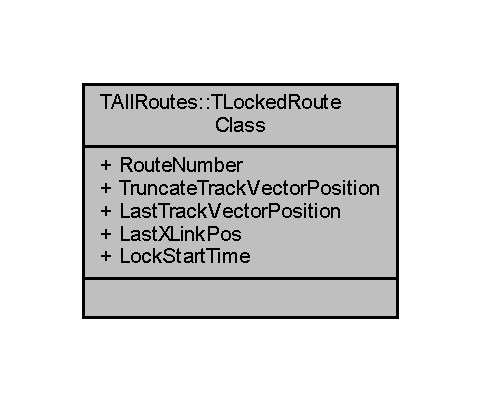
\includegraphics[width=231pt]{class_t_all_routes_1_1_t_locked_route_class__coll__graph}
\end{center}
\end{figure}
\subsection*{Public Attributes}
\begin{DoxyCompactItemize}
\item 
\mbox{\Hypertarget{class_t_all_routes_1_1_t_locked_route_class_a2656289cb7f1553d6189a03dda77fe16}\label{class_t_all_routes_1_1_t_locked_route_class_a2656289cb7f1553d6189a03dda77fe16}} 
int \mbox{\hyperlink{class_t_all_routes_1_1_t_locked_route_class_a2656289cb7f1553d6189a03dda77fe16}{Route\+Number}}
\begin{DoxyCompactList}\small\item\em the vector position number of the relevant route in All\+Routes\+Vector \end{DoxyCompactList}\item 
\mbox{\Hypertarget{class_t_all_routes_1_1_t_locked_route_class_a225d5505b6ec121e35defa4f228798f5}\label{class_t_all_routes_1_1_t_locked_route_class_a225d5505b6ec121e35defa4f228798f5}} 
unsigned int \mbox{\hyperlink{class_t_all_routes_1_1_t_locked_route_class_a225d5505b6ec121e35defa4f228798f5}{Truncate\+Track\+Vector\+Position}}
\begin{DoxyCompactList}\small\item\em the Track\+Vector position of the element selected for truncation \end{DoxyCompactList}\item 
\mbox{\Hypertarget{class_t_all_routes_1_1_t_locked_route_class_a9a989378c6e20fc0c68bbbebe87016c3}\label{class_t_all_routes_1_1_t_locked_route_class_a9a989378c6e20fc0c68bbbebe87016c3}} 
unsigned int \mbox{\hyperlink{class_t_all_routes_1_1_t_locked_route_class_a9a989378c6e20fc0c68bbbebe87016c3}{Last\+Track\+Vector\+Position}}
\begin{DoxyCompactList}\small\item\em the Track\+Vector position of the last (i.\+e. most forward) element in the route \end{DoxyCompactList}\item 
\mbox{\Hypertarget{class_t_all_routes_1_1_t_locked_route_class_acc5cb84f033b12d8216816b8a6a6c0a3}\label{class_t_all_routes_1_1_t_locked_route_class_acc5cb84f033b12d8216816b8a6a6c0a3}} 
int \mbox{\hyperlink{class_t_all_routes_1_1_t_locked_route_class_acc5cb84f033b12d8216816b8a6a6c0a3}{Last\+X\+Link\+Pos}}
\begin{DoxyCompactList}\small\item\em the X\+Link\+Pos value of the last (i.\+e. most forward) element in the route \end{DoxyCompactList}\item 
\mbox{\Hypertarget{class_t_all_routes_1_1_t_locked_route_class_a387fd30893416bd59e9f8719282c4f26}\label{class_t_all_routes_1_1_t_locked_route_class_a387fd30893416bd59e9f8719282c4f26}} 
T\+Date\+Time \mbox{\hyperlink{class_t_all_routes_1_1_t_locked_route_class_a387fd30893416bd59e9f8719282c4f26}{Lock\+Start\+Time}}
\begin{DoxyCompactList}\small\item\em the timetable time at which the route is locked, to start the 2 minute clock \end{DoxyCompactList}\end{DoxyCompactItemize}


\subsection{Detailed Description}
Handles routes that are locked because of approaching trains. 

The documentation for this class was generated from the following file\+:\begin{DoxyCompactItemize}
\item 
Track\+Unit.\+h\end{DoxyCompactItemize}

\hypertarget{class_t_map_comp}{}\section{T\+Map\+Comp Class Reference}
\label{class_t_map_comp}\index{T\+Map\+Comp@{T\+Map\+Comp}}


type only declared here to allow access, full declaration in Display\+Unit  




{\ttfamily \#include $<$Track\+Unit.\+h$>$}

\subsection*{Public Member Functions}
\begin{DoxyCompactItemize}
\item 
\mbox{\Hypertarget{class_t_map_comp_a6784886eff8452405709d93063d74147}\label{class_t_map_comp_a6784886eff8452405709d93063d74147}} 
bool \mbox{\hyperlink{class_t_map_comp_a6784886eff8452405709d93063d74147}{operator()}} (const T\+H\+V\+Pair \&lower, const T\+H\+V\+Pair \&higher) const
\begin{DoxyCompactList}\small\item\em H\+Loc V\+Loc. \end{DoxyCompactList}\end{DoxyCompactItemize}


\subsection{Detailed Description}
type only declared here to allow access, full declaration in Display\+Unit 

Map and multimap comparator based on horizontal \& vertical position 

The documentation for this class was generated from the following files\+:\begin{DoxyCompactItemize}
\item 
C\+:/\+Programming work/railway development after v2.\+2.\+0/Track\+Unit.\+h\item 
C\+:/\+Programming work/railway development after v2.\+2.\+0/Track\+Unit.\+cpp\end{DoxyCompactItemize}

\hypertarget{class_t_one_complete_formatted_train}{}\section{T\+One\+Complete\+Formatted\+Train Class Reference}
\label{class_t_one_complete_formatted_train}\index{T\+One\+Complete\+Formatted\+Train@{T\+One\+Complete\+Formatted\+Train}}


A single train with its headcode + list of actions for use in the formatted timetable.  




{\ttfamily \#include $<$Train\+Unit.\+h$>$}

\subsection*{Public Attributes}
\begin{DoxyCompactItemize}
\item 
\mbox{\Hypertarget{class_t_one_complete_formatted_train_a64e2c06ac8ceb57b8f2cf4fe316fdd09}\label{class_t_one_complete_formatted_train_a64e2c06ac8ceb57b8f2cf4fe316fdd09}} 
Ansi\+String {\bfseries Head\+Code}
\item 
\mbox{\Hypertarget{class_t_one_complete_formatted_train_a7153d13265831ee7c241779b5c803278}\label{class_t_one_complete_formatted_train_a7153d13265831ee7c241779b5c803278}} 
T\+One\+Formatted\+Train\+Vector \mbox{\hyperlink{class_t_one_complete_formatted_train_a7153d13265831ee7c241779b5c803278}{One\+Formatted\+Train\+Vector}}
\begin{DoxyCompactList}\small\item\em see above \end{DoxyCompactList}\end{DoxyCompactItemize}


\subsection{Detailed Description}
A single train with its headcode + list of actions for use in the formatted timetable. 

The documentation for this class was generated from the following file\+:\begin{DoxyCompactItemize}
\item 
C\+:/\+Programming work/railway development after v2.\+2.\+0/Train\+Unit.\+h\end{DoxyCompactItemize}

\hypertarget{class_t_one_pref_dir}{}\section{T\+One\+Pref\+Dir Class Reference}
\label{class_t_one_pref_dir}\index{T\+One\+Pref\+Dir@{T\+One\+Pref\+Dir}}


{\ttfamily \#include $<$Track\+Unit.\+h$>$}



Inheritance diagram for T\+One\+Pref\+Dir\+:\nopagebreak
\begin{figure}[H]
\begin{center}
\leavevmode
\includegraphics[height=550pt]{class_t_one_pref_dir__inherit__graph}
\end{center}
\end{figure}


Collaboration diagram for T\+One\+Pref\+Dir\+:\nopagebreak
\begin{figure}[H]
\begin{center}
\leavevmode
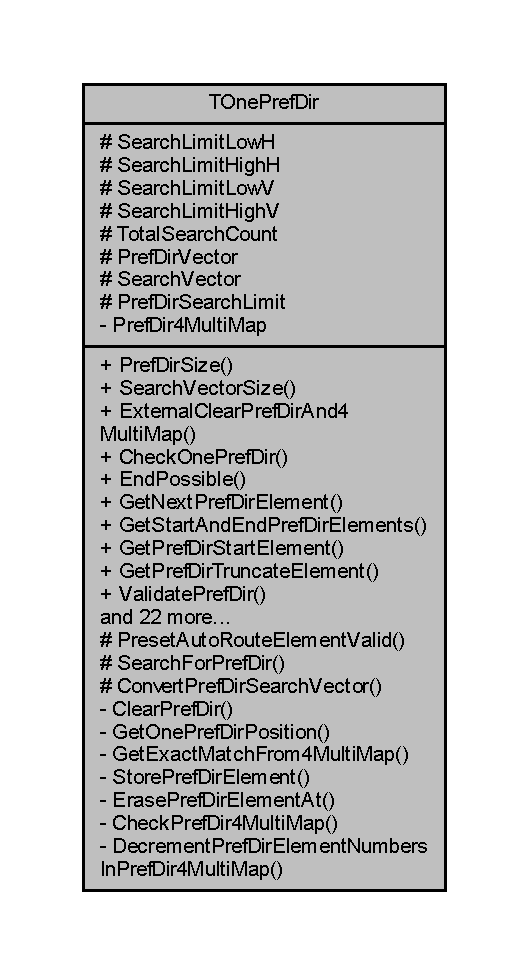
\includegraphics[width=254pt]{class_t_one_pref_dir__coll__graph}
\end{center}
\end{figure}
\subsection*{Public Member Functions}
\begin{DoxyCompactItemize}
\item 
\mbox{\Hypertarget{class_t_one_pref_dir_a29d013bf730e23d27fdb2c390e3a14da}\label{class_t_one_pref_dir_a29d013bf730e23d27fdb2c390e3a14da}} 
unsigned int \mbox{\hyperlink{class_t_one_pref_dir_a29d013bf730e23d27fdb2c390e3a14da}{Pref\+Dir\+Size}} () const
\begin{DoxyCompactList}\small\item\em Return the vector size. \end{DoxyCompactList}\item 
\mbox{\Hypertarget{class_t_one_pref_dir_a7a7fb4b5ae1ed73c9a989d21980d5b54}\label{class_t_one_pref_dir_a7a7fb4b5ae1ed73c9a989d21980d5b54}} 
unsigned int \mbox{\hyperlink{class_t_one_pref_dir_a7a7fb4b5ae1ed73c9a989d21980d5b54}{Search\+Vector\+Size}} () const
\begin{DoxyCompactList}\small\item\em Return the vector size. \end{DoxyCompactList}\item 
\mbox{\Hypertarget{class_t_one_pref_dir_abc09de3c32460a73d3de12625329210d}\label{class_t_one_pref_dir_abc09de3c32460a73d3de12625329210d}} 
void \mbox{\hyperlink{class_t_one_pref_dir_abc09de3c32460a73d3de12625329210d}{External\+Clear\+Pref\+Dir\+And4\+Multi\+Map}} ()
\begin{DoxyCompactList}\small\item\em Empty the existing preferred direction vector \& map -\/ for use by other classes. \end{DoxyCompactList}\item 
bool \mbox{\hyperlink{class_t_one_pref_dir_a1896affce3465b84cfd5128cca122639}{Check\+One\+Pref\+Dir}} (int Caller, int Number\+Of\+Active\+Elements, std\+::ifstream \&Vec\+File)
\item 
bool \mbox{\hyperlink{class_t_one_pref_dir_a7b81a1377e6269aafad6c25c929b2852}{End\+Possible}} (int Caller, bool \&Leading\+Points)
\item 
bool \mbox{\hyperlink{class_t_one_pref_dir_a06cd3491535362fccbba4e76b9a120e9}{Get\+Next\+Pref\+Dir\+Element}} (int Caller, int H\+Loc, int V\+Loc, bool \&Finish\+Element)
\item 
\mbox{\Hypertarget{class_t_one_pref_dir_a0acdc81183b894d1d6aecb5f563efefc}\label{class_t_one_pref_dir_a0acdc81183b894d1d6aecb5f563efefc}} 
bool \mbox{\hyperlink{class_t_one_pref_dir_a0acdc81183b894d1d6aecb5f563efefc}{Get\+Start\+And\+End\+Pref\+Dir\+Elements}} (int Caller, \mbox{\hyperlink{class_t_pref_dir_element}{T\+Pref\+Dir\+Element}} \&Start\+Element, \mbox{\hyperlink{class_t_pref_dir_element}{T\+Pref\+Dir\+Element}} \&End\+Element, int \&Last\+Iterator\+Value)
\begin{DoxyCompactList}\small\item\em Called when searching for start and end Pref\+Dir\+Elements when setting up automatic signals routes in Pre\+Start mode. \end{DoxyCompactList}\item 
bool \mbox{\hyperlink{class_t_one_pref_dir_ace0402792492c9da2551423f8287e41e}{Get\+Pref\+Dir\+Start\+Element}} (int Caller, int H\+Loc, int V\+Loc)
\item 
bool \mbox{\hyperlink{class_t_one_pref_dir_a8fd55282096fe63f0baeab323c6ccc8b}{Get\+Pref\+Dir\+Truncate\+Element}} (int Caller, int H\+Loc, int V\+Loc)
\item 
\mbox{\Hypertarget{class_t_one_pref_dir_a2b883633382e26cdff4583a24575d337}\label{class_t_one_pref_dir_a2b883633382e26cdff4583a24575d337}} 
bool \mbox{\hyperlink{class_t_one_pref_dir_a2b883633382e26cdff4583a24575d337}{Validate\+Pref\+Dir}} (int Caller)
\begin{DoxyCompactList}\small\item\em Checks that all elements in Pref\+Dir\+Vector have been properly set, i.\+e. don\textquotesingle{}t have their default values, and that every element is connected to the next element. \end{DoxyCompactList}\item 
\mbox{\Hypertarget{class_t_one_pref_dir_a26a1ee9d1ced0d53e35936097d4896f0}\label{class_t_one_pref_dir_a26a1ee9d1ced0d53e35936097d4896f0}} 
int \mbox{\hyperlink{class_t_one_pref_dir_a26a1ee9d1ced0d53e35936097d4896f0}{Last\+Element\+Number}} (int Caller) const
\begin{DoxyCompactList}\small\item\em Return the vector position of the last element in the vector (i.\+e. one less than the vector size) \end{DoxyCompactList}\item 
\mbox{\Hypertarget{class_t_one_pref_dir_a42862b2abcd0eb356982f4ce46922922}\label{class_t_one_pref_dir_a42862b2abcd0eb356982f4ce46922922}} 
T\+Pref\+Dir\+Vector\+Iterator \mbox{\hyperlink{class_t_one_pref_dir_a42862b2abcd0eb356982f4ce46922922}{Last\+Element\+Ptr}} (int Caller)
\begin{DoxyCompactList}\small\item\em Return a pointer to the last element in the vector. \end{DoxyCompactList}\item 
\mbox{\Hypertarget{class_t_one_pref_dir_a5b67e5aaa86d324229aedc68f32f32b8}\label{class_t_one_pref_dir_a5b67e5aaa86d324229aedc68f32f32b8}} 
const \mbox{\hyperlink{class_t_pref_dir_element}{T\+Pref\+Dir\+Element}} \& \mbox{\hyperlink{class_t_one_pref_dir_a5b67e5aaa86d324229aedc68f32f32b8}{Get\+Fixed\+Pref\+Dir\+Element\+At}} (int Caller, int At) const
\begin{DoxyCompactList}\small\item\em Return a non-\/modifiable element at Pref\+Dir\+Vector position \textquotesingle{}At\textquotesingle{}. \end{DoxyCompactList}\item 
\mbox{\Hypertarget{class_t_one_pref_dir_af5a2c955fa9c2584c683accbacb15f4c}\label{class_t_one_pref_dir_af5a2c955fa9c2584c683accbacb15f4c}} 
\mbox{\hyperlink{class_t_pref_dir_element}{T\+Pref\+Dir\+Element}} \& \mbox{\hyperlink{class_t_one_pref_dir_af5a2c955fa9c2584c683accbacb15f4c}{Get\+Modifiable\+Pref\+Dir\+Element\+At}} (int Caller, int At)
\begin{DoxyCompactList}\small\item\em Return a modifiable element at Pref\+Dir\+Vector position \textquotesingle{}At\textquotesingle{}. \end{DoxyCompactList}\item 
\mbox{\Hypertarget{class_t_one_pref_dir_a11543812cef66a28f4747fb3f8f33f47}\label{class_t_one_pref_dir_a11543812cef66a28f4747fb3f8f33f47}} 
const \mbox{\hyperlink{class_t_pref_dir_element}{T\+Pref\+Dir\+Element}} \& \mbox{\hyperlink{class_t_one_pref_dir_a11543812cef66a28f4747fb3f8f33f47}{Get\+Fixed\+Search\+Element\+At}} (int Caller, int At) const
\begin{DoxyCompactList}\small\item\em Return a non-\/modifiable element at Search\+Vector position \textquotesingle{}At\textquotesingle{}. \end{DoxyCompactList}\item 
\mbox{\Hypertarget{class_t_one_pref_dir_a6724a8304760eb6107bddc60a269595b}\label{class_t_one_pref_dir_a6724a8304760eb6107bddc60a269595b}} 
\mbox{\hyperlink{class_t_pref_dir_element}{T\+Pref\+Dir\+Element}} \& \mbox{\hyperlink{class_t_one_pref_dir_a6724a8304760eb6107bddc60a269595b}{Get\+Modifiable\+Search\+Element\+At}} (int Caller, int At)
\begin{DoxyCompactList}\small\item\em Return a modifiable element at Search\+Vector position \textquotesingle{}At\textquotesingle{}. \end{DoxyCompactList}\item 
void \mbox{\hyperlink{class_t_one_pref_dir_abadb0c99b24d6dbfda371d96b308fc6e}{Calc\+Distance\+And\+Speed}} (int Caller, int \&Overall\+Distance, int \&Overall\+Speed\+Limit, bool \&Leading\+Points\+At\+Last\+Element)
\item 
\mbox{\Hypertarget{class_t_one_pref_dir_a5e8d14c19c70cafe968e7481b116a714}\label{class_t_one_pref_dir_a5e8d14c19c70cafe968e7481b116a714}} 
void \mbox{\hyperlink{class_t_one_pref_dir_a5e8d14c19c70cafe968e7481b116a714}{External\+Store\+Pref\+Dir\+Element}} (int Caller, \mbox{\hyperlink{class_t_pref_dir_element}{T\+Pref\+Dir\+Element}} Load\+Pref\+Dir\+Element)
\begin{DoxyCompactList}\small\item\em Store a single pref dir element in the vector \& map -\/ used by other classes. \end{DoxyCompactList}\item 
\mbox{\Hypertarget{class_t_one_pref_dir_a820f6cc109de519289e6a63dac835ebc}\label{class_t_one_pref_dir_a820f6cc109de519289e6a63dac835ebc}} 
void \mbox{\hyperlink{class_t_one_pref_dir_a820f6cc109de519289e6a63dac835ebc}{Get\+Vector\+Positions\+From\+Pref\+Dir4\+Multi\+Map}} (int Caller, int H\+Loc, int V\+Loc, bool \&Found\+Flag, int \&Pref\+Dir\+Pos0, int \&Pref\+Dir\+Pos1, int \&Pref\+Dir\+Pos2, int \&Pref\+Dir\+Pos3)
\begin{DoxyCompactList}\small\item\em Return up to 4 vector positions for a given H\+Loc \& V\+Loc; unused values return -\/1. \end{DoxyCompactList}\item 
void \mbox{\hyperlink{class_t_one_pref_dir_a614933ff3958e4b8c9be9bc78159d9e8}{Load\+Old\+Pref\+Dir}} (int Caller, std\+::ifstream \&Vec\+File)
\item 
\mbox{\Hypertarget{class_t_one_pref_dir_a0779c9edd1ba268356590aac4719166d}\label{class_t_one_pref_dir_a0779c9edd1ba268356590aac4719166d}} 
void \mbox{\hyperlink{class_t_one_pref_dir_a0779c9edd1ba268356590aac4719166d}{Load\+Pref\+Dir}} (int Caller, std\+::ifstream \&Vec\+File)
\begin{DoxyCompactList}\small\item\em Load a vector and map of preferred directions from the file. \end{DoxyCompactList}\item 
void \mbox{\hyperlink{class_t_one_pref_dir_aef8388386635d73a921fae7ce43f5214}{Pref\+Dir\+Marker}} (int Caller, T\+Pref\+Dir\+Route Pref\+Dir\+Route, bool Building\+Pref\+Dir, \mbox{\hyperlink{class_t_display}{T\+Display}} $\ast$Disp) const
\item 
\mbox{\Hypertarget{class_t_one_pref_dir_a3d115535b2e2d2ea05e210997a3f525c}\label{class_t_one_pref_dir_a3d115535b2e2d2ea05e210997a3f525c}} 
void \mbox{\hyperlink{class_t_one_pref_dir_a3d115535b2e2d2ea05e210997a3f525c}{Save\+Pref\+Dir\+Vector}} (int Caller, std\+::ofstream \&Vec\+File)
\begin{DoxyCompactList}\small\item\em Save the preferred direction vector to a file. \end{DoxyCompactList}\item 
\mbox{\Hypertarget{class_t_one_pref_dir_a8871c609a1586aa9c4f723afaccd2502}\label{class_t_one_pref_dir_a8871c609a1586aa9c4f723afaccd2502}} 
void \mbox{\hyperlink{class_t_one_pref_dir_a8871c609a1586aa9c4f723afaccd2502}{Save\+Search\+Vector}} (int Caller, std\+::ofstream \&Vec\+File)
\begin{DoxyCompactList}\small\item\em Save the search vector to a file. \end{DoxyCompactList}\item 
\mbox{\Hypertarget{class_t_one_pref_dir_af87440e0ace47b20c8a874c51b314064}\label{class_t_one_pref_dir_af87440e0ace47b20c8a874c51b314064}} 
void \mbox{\hyperlink{class_t_one_pref_dir_af87440e0ace47b20c8a874c51b314064}{Write\+Pref\+Dir\+To\+Image}} (int Caller, Graphics\+::\+T\+Bitmap $\ast$Bitmap)
\begin{DoxyCompactList}\small\item\em Used when creating a bitmap image to display preferred directions (as on screen during \textquotesingle{}Set preferred direction\textquotesingle{} mode) \end{DoxyCompactList}\item 
bool \mbox{\hyperlink{class_t_one_pref_dir_ab8c8ad293f45948986903a05302b2dc8}{Check\+Pref\+Dir\+Against\+Track\+Vector\+No\+Message}} (int Caller)
\item 
void \mbox{\hyperlink{class_t_one_pref_dir_ab79dc3f93a471d2182ce625fcac1ff2d}{Check\+Pref\+Dir\+Against\+Track\+Vector}} (int Caller)
\item 
void \mbox{\hyperlink{class_t_one_pref_dir_a65df51092983945e1fe3c20bf8917a39}{Consolidate\+Pref\+Dirs}} (int Caller, \mbox{\hyperlink{class_t_one_pref_dir}{T\+One\+Pref\+Dir}} $\ast$Input\+Pref\+Dir)
\item 
void \mbox{\hyperlink{class_t_one_pref_dir_a8042c0e2fd7f9e39c3ca2a7bff7c68a4}{Erase\+From\+Pref\+Dir\+Vector\+And4\+Multi\+Map}} (int Caller, int H\+Loc, int V\+Loc)
\item 
void \mbox{\hyperlink{class_t_one_pref_dir_a9b425a3ed8ef998e2366d13ad52bf08c}{Every\+Pref\+Dir\+Marker}} (int Caller, \mbox{\hyperlink{class_t_display}{T\+Display}} $\ast$Disp)
\item 
void \mbox{\hyperlink{class_t_one_pref_dir_ab5bb3791670fd04645faf4ab1f2a5781}{Realign\+After\+Track\+Erase}} (int Caller, int Erased\+Track\+Vector\+Position)
\item 
void \mbox{\hyperlink{class_t_one_pref_dir_a1e62c2571d3629a067e1071086de72de}{Rebuild\+Pref\+Dir\+Vector}} (int Caller)
\end{DoxyCompactItemize}
\subsection*{Protected Types}
\begin{DoxyCompactItemize}
\item 
\mbox{\Hypertarget{class_t_one_pref_dir_a7162736e4bbe36fbac7a57ce395fcd14}\label{class_t_one_pref_dir_a7162736e4bbe36fbac7a57ce395fcd14}} 
typedef std\+::vector$<$ \mbox{\hyperlink{class_t_pref_dir_element}{T\+Pref\+Dir\+Element}} $>$ \mbox{\hyperlink{class_t_one_pref_dir_a7162736e4bbe36fbac7a57ce395fcd14}{T\+Pref\+Dir\+Vector}}
\begin{DoxyCompactList}\small\item\em the pref dir vector type \end{DoxyCompactList}\item 
\mbox{\Hypertarget{class_t_one_pref_dir_a8a905cfdce2439be93d45b66339b7382}\label{class_t_one_pref_dir_a8a905cfdce2439be93d45b66339b7382}} 
typedef std\+::vector$<$ \mbox{\hyperlink{class_t_pref_dir_element}{T\+Pref\+Dir\+Element}} $>$\+::iterator {\bfseries T\+Pref\+Dir\+Vector\+Iterator}
\item 
\mbox{\Hypertarget{class_t_one_pref_dir_a53624ed7b429b42aa57cfe5551f5df71}\label{class_t_one_pref_dir_a53624ed7b429b42aa57cfe5551f5df71}} 
typedef std\+::vector$<$ \mbox{\hyperlink{class_t_pref_dir_element}{T\+Pref\+Dir\+Element}} $>$\+::const\+\_\+iterator {\bfseries T\+Pref\+Dir\+Vector\+Const\+Iterator}
\end{DoxyCompactItemize}
\subsection*{Protected Member Functions}
\begin{DoxyCompactItemize}
\item 
bool \mbox{\hyperlink{class_t_one_pref_dir_ab35c683ba0ec156d19d4db991046b7d2}{Preset\+Auto\+Route\+Element\+Valid}} (int Caller, \mbox{\hyperlink{class_t_pref_dir_element}{T\+Pref\+Dir\+Element}} Element\+In, int Entry\+Pos)
\item 
bool \mbox{\hyperlink{class_t_one_pref_dir_a82c6a19d67ada7059491afae05ced4a4}{Search\+For\+Pref\+Dir}} (int Caller, \mbox{\hyperlink{class_t_track_element}{T\+Track\+Element}} Track\+Element, int X\+Link\+Pos, int Required\+Position)
\item 
\mbox{\Hypertarget{class_t_one_pref_dir_a482d1c69a674eec4db0190b78659c495}\label{class_t_one_pref_dir_a482d1c69a674eec4db0190b78659c495}} 
void \mbox{\hyperlink{class_t_one_pref_dir_a482d1c69a674eec4db0190b78659c495}{Convert\+Pref\+Dir\+Search\+Vector}} (int Caller)
\begin{DoxyCompactList}\small\item\em Called after a successful search to add the elements from the search vector to the pref dir vector. \end{DoxyCompactList}\end{DoxyCompactItemize}
\subsection*{Protected Attributes}
\begin{DoxyCompactItemize}
\item 
\mbox{\Hypertarget{class_t_one_pref_dir_af33d48762fe2b104b75fca9a97d96252}\label{class_t_one_pref_dir_af33d48762fe2b104b75fca9a97d96252}} 
int {\bfseries Search\+Limit\+LowH}
\item 
\mbox{\Hypertarget{class_t_one_pref_dir_a68677f0598c54c3e6e3c27075b23aa14}\label{class_t_one_pref_dir_a68677f0598c54c3e6e3c27075b23aa14}} 
int {\bfseries Search\+Limit\+HighH}
\item 
\mbox{\Hypertarget{class_t_one_pref_dir_aa469479759bd4379bee3f938ad8bfd90}\label{class_t_one_pref_dir_aa469479759bd4379bee3f938ad8bfd90}} 
int {\bfseries Search\+Limit\+LowV}
\item 
\mbox{\Hypertarget{class_t_one_pref_dir_a2665c08fe2a230db10ded6e78975bc13}\label{class_t_one_pref_dir_a2665c08fe2a230db10ded6e78975bc13}} 
int {\bfseries Search\+Limit\+HighV}
\item 
\mbox{\Hypertarget{class_t_one_pref_dir_a8e982d8317ce1579b143adf74d88d692}\label{class_t_one_pref_dir_a8e982d8317ce1579b143adf74d88d692}} 
int \mbox{\hyperlink{class_t_one_pref_dir_a8e982d8317ce1579b143adf74d88d692}{Total\+Search\+Count}}
\begin{DoxyCompactList}\small\item\em counts search elements, used to abort searches (prefdirs or routes) if reaches too high a value \end{DoxyCompactList}\item 
\mbox{\Hypertarget{class_t_one_pref_dir_ab2da871d689df7e78f430c5d354bb953}\label{class_t_one_pref_dir_ab2da871d689df7e78f430c5d354bb953}} 
\mbox{\hyperlink{class_t_one_pref_dir_a7162736e4bbe36fbac7a57ce395fcd14}{T\+Pref\+Dir\+Vector}} {\bfseries Pref\+Dir\+Vector}
\item 
\mbox{\Hypertarget{class_t_one_pref_dir_a2d035366a044fc7d0e0a745762bd4664}\label{class_t_one_pref_dir_a2d035366a044fc7d0e0a745762bd4664}} 
\mbox{\hyperlink{class_t_one_pref_dir_a7162736e4bbe36fbac7a57ce395fcd14}{T\+Pref\+Dir\+Vector}} \mbox{\hyperlink{class_t_one_pref_dir_a2d035366a044fc7d0e0a745762bd4664}{Search\+Vector}}
\begin{DoxyCompactList}\small\item\em pref dir vectors, first is the main vector, second used to store search elements temporarily \end{DoxyCompactList}\end{DoxyCompactItemize}
\subsection*{Static Protected Attributes}
\begin{DoxyCompactItemize}
\item 
\mbox{\Hypertarget{class_t_one_pref_dir_a9fc8032fb9c525951620e7aafa067d45}\label{class_t_one_pref_dir_a9fc8032fb9c525951620e7aafa067d45}} 
static const int \mbox{\hyperlink{class_t_one_pref_dir_a9fc8032fb9c525951620e7aafa067d45}{Pref\+Dir\+Search\+Limit}} = 30000
\begin{DoxyCompactList}\small\item\em limit to the number of elements searched in attempting to find a preferred direction \end{DoxyCompactList}\end{DoxyCompactItemize}
\subsection*{Private Types}
\begin{DoxyCompactItemize}
\item 
\mbox{\Hypertarget{class_t_one_pref_dir_a940ba2bdbedb288c8188c1da5c4c79bc}\label{class_t_one_pref_dir_a940ba2bdbedb288c8188c1da5c4c79bc}} 
typedef std\+::multimap$<$ T\+H\+V\+Pair, unsigned int, \mbox{\hyperlink{class_t_map_comp}{T\+Map\+Comp}} $>$ \mbox{\hyperlink{class_t_one_pref_dir_a940ba2bdbedb288c8188c1da5c4c79bc}{T\+Pref\+Dir4\+Multi\+Map}}
\begin{DoxyCompactList}\small\item\em H\+Loc\&V\+Loc as a pair, and Pref\+Dir\+Vector\+Position, can be up to 4 values at any H\&V. \end{DoxyCompactList}\item 
\mbox{\Hypertarget{class_t_one_pref_dir_a37efac41fc00465b0569704517233d4e}\label{class_t_one_pref_dir_a37efac41fc00465b0569704517233d4e}} 
typedef std\+::multimap$<$ T\+H\+V\+Pair, unsigned int, \mbox{\hyperlink{class_t_map_comp}{T\+Map\+Comp}} $>$\+::iterator {\bfseries T\+Pref\+Dir4\+Multi\+Map\+Iterator}
\item 
\mbox{\Hypertarget{class_t_one_pref_dir_a05da09493d511df74b8e5b9a794c2e0b}\label{class_t_one_pref_dir_a05da09493d511df74b8e5b9a794c2e0b}} 
typedef std\+::pair$<$ T\+H\+V\+Pair, unsigned int $>$ {\bfseries T\+Pref\+Dir4\+Multi\+Map\+Entry}
\end{DoxyCompactItemize}
\subsection*{Private Member Functions}
\begin{DoxyCompactItemize}
\item 
\mbox{\Hypertarget{class_t_one_pref_dir_ad2e6adb7b634b17cab9cd03610a0f8e3}\label{class_t_one_pref_dir_ad2e6adb7b634b17cab9cd03610a0f8e3}} 
void \mbox{\hyperlink{class_t_one_pref_dir_ad2e6adb7b634b17cab9cd03610a0f8e3}{Clear\+Pref\+Dir}} ()
\begin{DoxyCompactList}\small\item\em Empty the existing vectors \& map. \end{DoxyCompactList}\item 
int \mbox{\hyperlink{class_t_one_pref_dir_a200fd1dc1cffc400160b8d2147278752}{Get\+One\+Pref\+Dir\+Position}} (int Caller, int H\+Loc, int V\+Loc)
\item 
T\+Pref\+Dir4\+Multi\+Map\+Iterator \mbox{\hyperlink{class_t_one_pref_dir_a8bc65b139325c45b57a9f43a9b3404a8}{Get\+Exact\+Match\+From4\+Multi\+Map}} (int Caller, unsigned int Pref\+Dir\+Vector\+Position, bool \&Found\+Flag)
\item 
\mbox{\Hypertarget{class_t_one_pref_dir_ac5f8d2864f0510cf73cb9883b520ec9f}\label{class_t_one_pref_dir_ac5f8d2864f0510cf73cb9883b520ec9f}} 
void \mbox{\hyperlink{class_t_one_pref_dir_ac5f8d2864f0510cf73cb9883b520ec9f}{Store\+Pref\+Dir\+Element}} (int Caller, \mbox{\hyperlink{class_t_pref_dir_element}{T\+Pref\+Dir\+Element}} Load\+Pref\+Dir\+Element)
\begin{DoxyCompactList}\small\item\em Store a single pref dir element in the vector \& map. \end{DoxyCompactList}\item 
void \mbox{\hyperlink{class_t_one_pref_dir_aa191ffa7fa23838043d34d9b02cd7bcb}{Erase\+Pref\+Dir\+Element\+At}} (int Caller, int Pref\+Dir\+Vector\+Position)
\item 
\mbox{\Hypertarget{class_t_one_pref_dir_a8a7ddf3981800ec0df1225c9e5aa52c2}\label{class_t_one_pref_dir_a8a7ddf3981800ec0df1225c9e5aa52c2}} 
void \mbox{\hyperlink{class_t_one_pref_dir_a8a7ddf3981800ec0df1225c9e5aa52c2}{Check\+Pref\+Dir4\+Multi\+Map}} (int Caller)
\begin{DoxyCompactList}\small\item\em Diagnostic validity check. \end{DoxyCompactList}\item 
\mbox{\Hypertarget{class_t_one_pref_dir_a056c475541b487ce13cb34dc43b1cf6f}\label{class_t_one_pref_dir_a056c475541b487ce13cb34dc43b1cf6f}} 
void \mbox{\hyperlink{class_t_one_pref_dir_a056c475541b487ce13cb34dc43b1cf6f}{Decrement\+Pref\+Dir\+Element\+Numbers\+In\+Pref\+Dir4\+Multi\+Map}} (int Caller, unsigned int Erased\+Element\+Number)
\begin{DoxyCompactList}\small\item\em Called after Erase\+Pref\+Dir\+Element\+At to decrement the remaining Pref\+Dir\+Element\+Numbers in 4\+Multi\+Map if they are greater than the erased value. \end{DoxyCompactList}\end{DoxyCompactItemize}
\subsection*{Private Attributes}
\begin{DoxyCompactItemize}
\item 
\mbox{\Hypertarget{class_t_one_pref_dir_aa6738f8f24fe0a417a84388c049b5e4c}\label{class_t_one_pref_dir_aa6738f8f24fe0a417a84388c049b5e4c}} 
\mbox{\hyperlink{class_t_one_pref_dir_a940ba2bdbedb288c8188c1da5c4c79bc}{T\+Pref\+Dir4\+Multi\+Map}} \mbox{\hyperlink{class_t_one_pref_dir_aa6738f8f24fe0a417a84388c049b5e4c}{Pref\+Dir4\+Multi\+Map}}
\begin{DoxyCompactList}\small\item\em the pref dir multimap -\/ up to 4 values (up to 2 tracks per element each with 2 directions) \end{DoxyCompactList}\end{DoxyCompactItemize}


\subsection{Detailed Description}
The basic preferred direction class, consisting of any number of elements with preferred directions set.

Used during setting up preferred directions and track lengths (Construct\+Pref\+Dir), and for all completed preferred directions in the railway (Every\+Pref\+Dir) 

\subsection{Member Function Documentation}
\mbox{\Hypertarget{class_t_one_pref_dir_abadb0c99b24d6dbfda371d96b308fc6e}\label{class_t_one_pref_dir_abadb0c99b24d6dbfda371d96b308fc6e}} 
\index{T\+One\+Pref\+Dir@{T\+One\+Pref\+Dir}!Calc\+Distance\+And\+Speed@{Calc\+Distance\+And\+Speed}}
\index{Calc\+Distance\+And\+Speed@{Calc\+Distance\+And\+Speed}!T\+One\+Pref\+Dir@{T\+One\+Pref\+Dir}}
\subsubsection{\texorpdfstring{Calc\+Distance\+And\+Speed()}{CalcDistanceAndSpeed()}}
{\footnotesize\ttfamily void T\+One\+Pref\+Dir\+::\+Calc\+Distance\+And\+Speed (\begin{DoxyParamCaption}\item[{int}]{Caller,  }\item[{int \&}]{Overall\+Distance,  }\item[{int \&}]{Overall\+Speed\+Limit,  }\item[{bool \&}]{Leading\+Points\+At\+Last\+Element }\end{DoxyParamCaption})}

Used when setting element lengths, returns in \&Overall\+Distance the overall distance for the selected chain of elements and also the speed limit in \&Overall\+Speed\+Limit, which is set to -\/1 if the speed limits vary over the chain \mbox{\Hypertarget{class_t_one_pref_dir_a1896affce3465b84cfd5128cca122639}\label{class_t_one_pref_dir_a1896affce3465b84cfd5128cca122639}} 
\index{T\+One\+Pref\+Dir@{T\+One\+Pref\+Dir}!Check\+One\+Pref\+Dir@{Check\+One\+Pref\+Dir}}
\index{Check\+One\+Pref\+Dir@{Check\+One\+Pref\+Dir}!T\+One\+Pref\+Dir@{T\+One\+Pref\+Dir}}
\subsubsection{\texorpdfstring{Check\+One\+Pref\+Dir()}{CheckOnePrefDir()}}
{\footnotesize\ttfamily bool T\+One\+Pref\+Dir\+::\+Check\+One\+Pref\+Dir (\begin{DoxyParamCaption}\item[{int}]{Caller,  }\item[{int}]{Number\+Of\+Active\+Elements,  }\item[{std\+::ifstream \&}]{Vec\+File }\end{DoxyParamCaption})}

Called before Pref\+Dir loading as part of the File\+Integrity\+Check function in case there is an error in the file. Very similar to Load\+Pref\+Dir but with value checks instead of storage in Pref\+Dir\+Vector. \mbox{\Hypertarget{class_t_one_pref_dir_ab79dc3f93a471d2182ce625fcac1ff2d}\label{class_t_one_pref_dir_ab79dc3f93a471d2182ce625fcac1ff2d}} 
\index{T\+One\+Pref\+Dir@{T\+One\+Pref\+Dir}!Check\+Pref\+Dir\+Against\+Track\+Vector@{Check\+Pref\+Dir\+Against\+Track\+Vector}}
\index{Check\+Pref\+Dir\+Against\+Track\+Vector@{Check\+Pref\+Dir\+Against\+Track\+Vector}!T\+One\+Pref\+Dir@{T\+One\+Pref\+Dir}}
\subsubsection{\texorpdfstring{Check\+Pref\+Dir\+Against\+Track\+Vector()}{CheckPrefDirAgainstTrackVector()}}
{\footnotesize\ttfamily void T\+One\+Pref\+Dir\+::\+Check\+Pref\+Dir\+Against\+Track\+Vector (\begin{DoxyParamCaption}\item[{int}]{Caller }\end{DoxyParamCaption})}

Check loaded Pref\+Dir against loaded track, and if discrepancies found give message \& clear Every\+Pref\+Dir \& Pref\+Dir4\+Multi\+Map. \mbox{\Hypertarget{class_t_one_pref_dir_ab8c8ad293f45948986903a05302b2dc8}\label{class_t_one_pref_dir_ab8c8ad293f45948986903a05302b2dc8}} 
\index{T\+One\+Pref\+Dir@{T\+One\+Pref\+Dir}!Check\+Pref\+Dir\+Against\+Track\+Vector\+No\+Message@{Check\+Pref\+Dir\+Against\+Track\+Vector\+No\+Message}}
\index{Check\+Pref\+Dir\+Against\+Track\+Vector\+No\+Message@{Check\+Pref\+Dir\+Against\+Track\+Vector\+No\+Message}!T\+One\+Pref\+Dir@{T\+One\+Pref\+Dir}}
\subsubsection{\texorpdfstring{Check\+Pref\+Dir\+Against\+Track\+Vector\+No\+Message()}{CheckPrefDirAgainstTrackVectorNoMessage()}}
{\footnotesize\ttfamily bool T\+One\+Pref\+Dir\+::\+Check\+Pref\+Dir\+Against\+Track\+Vector\+No\+Message (\begin{DoxyParamCaption}\item[{int}]{Caller }\end{DoxyParamCaption})}

Check loaded Pref\+Dir against loaded track, and if discrepancies found clear Every\+Pref\+Dir \& Pref\+Dir4\+Multi\+Map, messages are given by the calling routine. Return true for OK \mbox{\Hypertarget{class_t_one_pref_dir_a65df51092983945e1fe3c20bf8917a39}\label{class_t_one_pref_dir_a65df51092983945e1fe3c20bf8917a39}} 
\index{T\+One\+Pref\+Dir@{T\+One\+Pref\+Dir}!Consolidate\+Pref\+Dirs@{Consolidate\+Pref\+Dirs}}
\index{Consolidate\+Pref\+Dirs@{Consolidate\+Pref\+Dirs}!T\+One\+Pref\+Dir@{T\+One\+Pref\+Dir}}
\subsubsection{\texorpdfstring{Consolidate\+Pref\+Dirs()}{ConsolidatePrefDirs()}}
{\footnotesize\ttfamily void T\+One\+Pref\+Dir\+::\+Consolidate\+Pref\+Dirs (\begin{DoxyParamCaption}\item[{int}]{Caller,  }\item[{\mbox{\hyperlink{class_t_one_pref_dir}{T\+One\+Pref\+Dir}} $\ast$}]{Input\+Pref\+Dir }\end{DoxyParamCaption})}

Used when a preferred direction has been set to add all the elements to Every\+Pref\+Dir, except when they already exist in Every\+Pref\+Dir \mbox{\Hypertarget{class_t_one_pref_dir_a7b81a1377e6269aafad6c25c929b2852}\label{class_t_one_pref_dir_a7b81a1377e6269aafad6c25c929b2852}} 
\index{T\+One\+Pref\+Dir@{T\+One\+Pref\+Dir}!End\+Possible@{End\+Possible}}
\index{End\+Possible@{End\+Possible}!T\+One\+Pref\+Dir@{T\+One\+Pref\+Dir}}
\subsubsection{\texorpdfstring{End\+Possible()}{EndPossible()}}
{\footnotesize\ttfamily bool T\+One\+Pref\+Dir\+::\+End\+Possible (\begin{DoxyParamCaption}\item[{int}]{Caller,  }\item[{bool \&}]{Leading\+Points }\end{DoxyParamCaption})}

Used when setting preferred directions, true if able to finish at the last selected element (can\textquotesingle{}t finish if there is only one element or if end on leading points) \mbox{\Hypertarget{class_t_one_pref_dir_a8042c0e2fd7f9e39c3ca2a7bff7c68a4}\label{class_t_one_pref_dir_a8042c0e2fd7f9e39c3ca2a7bff7c68a4}} 
\index{T\+One\+Pref\+Dir@{T\+One\+Pref\+Dir}!Erase\+From\+Pref\+Dir\+Vector\+And4\+Multi\+Map@{Erase\+From\+Pref\+Dir\+Vector\+And4\+Multi\+Map}}
\index{Erase\+From\+Pref\+Dir\+Vector\+And4\+Multi\+Map@{Erase\+From\+Pref\+Dir\+Vector\+And4\+Multi\+Map}!T\+One\+Pref\+Dir@{T\+One\+Pref\+Dir}}
\subsubsection{\texorpdfstring{Erase\+From\+Pref\+Dir\+Vector\+And4\+Multi\+Map()}{EraseFromPrefDirVectorAnd4MultiMap()}}
{\footnotesize\ttfamily void T\+One\+Pref\+Dir\+::\+Erase\+From\+Pref\+Dir\+Vector\+And4\+Multi\+Map (\begin{DoxyParamCaption}\item[{int}]{Caller,  }\item[{int}]{H\+Loc,  }\item[{int}]{V\+Loc }\end{DoxyParamCaption})}

Erase element at H\+Loc and V\+Loc from the Pref\+Dir\+Vector and from the 4\+Multi\+Map. Note that this entails erasing up to four elements (2 directions and 2 tracks for 4-\/entry elements). \mbox{\Hypertarget{class_t_one_pref_dir_aa191ffa7fa23838043d34d9b02cd7bcb}\label{class_t_one_pref_dir_aa191ffa7fa23838043d34d9b02cd7bcb}} 
\index{T\+One\+Pref\+Dir@{T\+One\+Pref\+Dir}!Erase\+Pref\+Dir\+Element\+At@{Erase\+Pref\+Dir\+Element\+At}}
\index{Erase\+Pref\+Dir\+Element\+At@{Erase\+Pref\+Dir\+Element\+At}!T\+One\+Pref\+Dir@{T\+One\+Pref\+Dir}}
\subsubsection{\texorpdfstring{Erase\+Pref\+Dir\+Element\+At()}{ErasePrefDirElementAt()}}
{\footnotesize\ttfamily void T\+One\+Pref\+Dir\+::\+Erase\+Pref\+Dir\+Element\+At (\begin{DoxyParamCaption}\item[{int}]{Caller,  }\item[{int}]{Pref\+Dir\+Vector\+Position }\end{DoxyParamCaption})\hspace{0.3cm}{\ttfamily [private]}}

Erase a single element from Pref\+Dir\+Vector and 4\+Multi\+Map, decrementing the remaining Pref\+Dir\+Element\+Numbers in 4\+Multi\+Map if they are greater than the erased value. \mbox{\Hypertarget{class_t_one_pref_dir_a9b425a3ed8ef998e2366d13ad52bf08c}\label{class_t_one_pref_dir_a9b425a3ed8ef998e2366d13ad52bf08c}} 
\index{T\+One\+Pref\+Dir@{T\+One\+Pref\+Dir}!Every\+Pref\+Dir\+Marker@{Every\+Pref\+Dir\+Marker}}
\index{Every\+Pref\+Dir\+Marker@{Every\+Pref\+Dir\+Marker}!T\+One\+Pref\+Dir@{T\+One\+Pref\+Dir}}
\subsubsection{\texorpdfstring{Every\+Pref\+Dir\+Marker()}{EveryPrefDirMarker()}}
{\footnotesize\ttfamily void T\+One\+Pref\+Dir\+::\+Every\+Pref\+Dir\+Marker (\begin{DoxyParamCaption}\item[{int}]{Caller,  }\item[{\mbox{\hyperlink{class_t_display}{T\+Display}} $\ast$}]{Disp }\end{DoxyParamCaption})}

Similar to Pref\+Dir\+Marker but used only to mark Every\+Pref\+Dir -\/ red for unidirectional Pref\+Dir \& green for bidirectional. Colours taken from the route colours. Plot red first so green overwrites for bidirectional points. \mbox{\Hypertarget{class_t_one_pref_dir_a8bc65b139325c45b57a9f43a9b3404a8}\label{class_t_one_pref_dir_a8bc65b139325c45b57a9f43a9b3404a8}} 
\index{T\+One\+Pref\+Dir@{T\+One\+Pref\+Dir}!Get\+Exact\+Match\+From4\+Multi\+Map@{Get\+Exact\+Match\+From4\+Multi\+Map}}
\index{Get\+Exact\+Match\+From4\+Multi\+Map@{Get\+Exact\+Match\+From4\+Multi\+Map}!T\+One\+Pref\+Dir@{T\+One\+Pref\+Dir}}
\subsubsection{\texorpdfstring{Get\+Exact\+Match\+From4\+Multi\+Map()}{GetExactMatchFrom4MultiMap()}}
{\footnotesize\ttfamily T\+One\+Pref\+Dir\+::\+T\+Pref\+Dir4\+Multi\+Map\+Iterator T\+One\+Pref\+Dir\+::\+Get\+Exact\+Match\+From4\+Multi\+Map (\begin{DoxyParamCaption}\item[{int}]{Caller,  }\item[{unsigned int}]{Pref\+Dir\+Vector\+Position,  }\item[{bool \&}]{Found\+Flag }\end{DoxyParamCaption})\hspace{0.3cm}{\ttfamily [private]}}

Retrieves a Pref\+Dir4\+Multi\+Map iterator to the Pref\+Dir element at Pref\+Dir\+Vector\+Position. Used during Erase\+Pref\+Dir\+Element\+At to erase the relevant element in the multimap. If nothing is found this is an error but the error message is given in the calling function. \mbox{\Hypertarget{class_t_one_pref_dir_a06cd3491535362fccbba4e76b9a120e9}\label{class_t_one_pref_dir_a06cd3491535362fccbba4e76b9a120e9}} 
\index{T\+One\+Pref\+Dir@{T\+One\+Pref\+Dir}!Get\+Next\+Pref\+Dir\+Element@{Get\+Next\+Pref\+Dir\+Element}}
\index{Get\+Next\+Pref\+Dir\+Element@{Get\+Next\+Pref\+Dir\+Element}!T\+One\+Pref\+Dir@{T\+One\+Pref\+Dir}}
\subsubsection{\texorpdfstring{Get\+Next\+Pref\+Dir\+Element()}{GetNextPrefDirElement()}}
{\footnotesize\ttfamily bool T\+One\+Pref\+Dir\+::\+Get\+Next\+Pref\+Dir\+Element (\begin{DoxyParamCaption}\item[{int}]{Caller,  }\item[{int}]{H\+Loc,  }\item[{int}]{V\+Loc,  }\item[{bool \&}]{Finish\+Element }\end{DoxyParamCaption})}

Used when continuing a chain of preferred directions or element lengths. Tries to find a set of linked tracks between the last selected element and the one at H\+Loc \& V\+Loc, and returns true if it finds one. Finish\+Element is returned true if the element selected is a buffer or continuation -\/ in which case the chain is complete \mbox{\Hypertarget{class_t_one_pref_dir_a200fd1dc1cffc400160b8d2147278752}\label{class_t_one_pref_dir_a200fd1dc1cffc400160b8d2147278752}} 
\index{T\+One\+Pref\+Dir@{T\+One\+Pref\+Dir}!Get\+One\+Pref\+Dir\+Position@{Get\+One\+Pref\+Dir\+Position}}
\index{Get\+One\+Pref\+Dir\+Position@{Get\+One\+Pref\+Dir\+Position}!T\+One\+Pref\+Dir@{T\+One\+Pref\+Dir}}
\subsubsection{\texorpdfstring{Get\+One\+Pref\+Dir\+Position()}{GetOnePrefDirPosition()}}
{\footnotesize\ttfamily int T\+One\+Pref\+Dir\+::\+Get\+One\+Pref\+Dir\+Position (\begin{DoxyParamCaption}\item[{int}]{Caller,  }\item[{int}]{H\+Loc,  }\item[{int}]{V\+Loc }\end{DoxyParamCaption})\hspace{0.3cm}{\ttfamily [private]}}

Although there may be up to four entries at one H \& V position this function gets just one. It is used in Erase\+From\+Pref\+Dir\+Vector\+And4\+Multi\+Map by being called as many times as there are Pref\+Dir elements at H \& V. \mbox{\Hypertarget{class_t_one_pref_dir_ace0402792492c9da2551423f8287e41e}\label{class_t_one_pref_dir_ace0402792492c9da2551423f8287e41e}} 
\index{T\+One\+Pref\+Dir@{T\+One\+Pref\+Dir}!Get\+Pref\+Dir\+Start\+Element@{Get\+Pref\+Dir\+Start\+Element}}
\index{Get\+Pref\+Dir\+Start\+Element@{Get\+Pref\+Dir\+Start\+Element}!T\+One\+Pref\+Dir@{T\+One\+Pref\+Dir}}
\subsubsection{\texorpdfstring{Get\+Pref\+Dir\+Start\+Element()}{GetPrefDirStartElement()}}
{\footnotesize\ttfamily bool T\+One\+Pref\+Dir\+::\+Get\+Pref\+Dir\+Start\+Element (\begin{DoxyParamCaption}\item[{int}]{Caller,  }\item[{int}]{H\+Loc,  }\item[{int}]{V\+Loc }\end{DoxyParamCaption})}

Used when beginning a chain of preferred directions or element lengths. Enter with H\+Loc \& V\+Loc set to selected element \& check if selected element is a valid track element, return false if not, if it is, store it as the first entry in Pref\+Dir\+Vector and return true \mbox{\Hypertarget{class_t_one_pref_dir_a8fd55282096fe63f0baeab323c6ccc8b}\label{class_t_one_pref_dir_a8fd55282096fe63f0baeab323c6ccc8b}} 
\index{T\+One\+Pref\+Dir@{T\+One\+Pref\+Dir}!Get\+Pref\+Dir\+Truncate\+Element@{Get\+Pref\+Dir\+Truncate\+Element}}
\index{Get\+Pref\+Dir\+Truncate\+Element@{Get\+Pref\+Dir\+Truncate\+Element}!T\+One\+Pref\+Dir@{T\+One\+Pref\+Dir}}
\subsubsection{\texorpdfstring{Get\+Pref\+Dir\+Truncate\+Element()}{GetPrefDirTruncateElement()}}
{\footnotesize\ttfamily bool T\+One\+Pref\+Dir\+::\+Get\+Pref\+Dir\+Truncate\+Element (\begin{DoxyParamCaption}\item[{int}]{Caller,  }\item[{int}]{H\+Loc,  }\item[{int}]{V\+Loc }\end{DoxyParamCaption})}

Called during Pref\+Dir build or distance setting. It truncates at \& including the first element in the Pref\+Dir vector that matches H \& V. After the truncate the final element of the remaining Pref\+Dir has its data members reset to the same defaults as would be the case if the Pref\+Dir had been built up to that point -\/ i.\+e. for first element or a leading point. \mbox{\Hypertarget{class_t_one_pref_dir_a614933ff3958e4b8c9be9bc78159d9e8}\label{class_t_one_pref_dir_a614933ff3958e4b8c9be9bc78159d9e8}} 
\index{T\+One\+Pref\+Dir@{T\+One\+Pref\+Dir}!Load\+Old\+Pref\+Dir@{Load\+Old\+Pref\+Dir}}
\index{Load\+Old\+Pref\+Dir@{Load\+Old\+Pref\+Dir}!T\+One\+Pref\+Dir@{T\+One\+Pref\+Dir}}
\subsubsection{\texorpdfstring{Load\+Old\+Pref\+Dir()}{LoadOldPrefDir()}}
{\footnotesize\ttfamily void T\+One\+Pref\+Dir\+::\+Load\+Old\+Pref\+Dir (\begin{DoxyParamCaption}\item[{int}]{Caller,  }\item[{std\+::ifstream \&}]{Vec\+File }\end{DoxyParamCaption})}

Old version of Load\+Pref\+Dir, used during development when the save format changed so the old files could be loaded prior to resaving in the new format \mbox{\Hypertarget{class_t_one_pref_dir_aef8388386635d73a921fae7ce43f5214}\label{class_t_one_pref_dir_aef8388386635d73a921fae7ce43f5214}} 
\index{T\+One\+Pref\+Dir@{T\+One\+Pref\+Dir}!Pref\+Dir\+Marker@{Pref\+Dir\+Marker}}
\index{Pref\+Dir\+Marker@{Pref\+Dir\+Marker}!T\+One\+Pref\+Dir@{T\+One\+Pref\+Dir}}
\subsubsection{\texorpdfstring{Pref\+Dir\+Marker()}{PrefDirMarker()}}
{\footnotesize\ttfamily void T\+One\+Pref\+Dir\+::\+Pref\+Dir\+Marker (\begin{DoxyParamCaption}\item[{int}]{Caller,  }\item[{T\+Pref\+Dir\+Route}]{Pref\+Dir\+Route,  }\item[{bool}]{Building\+Pref\+Dir,  }\item[{\mbox{\hyperlink{class_t_display}{T\+Display}} $\ast$}]{Disp }\end{DoxyParamCaption}) const}

Pref\+Dir and route track marker, including direction markers. Function used for both Pref\+Dirs (Pref\+Dir\+Route == Pref\+Dir\+Call) and routes (Pref\+Dir\+Route == Route\+Call).

The graphics for marker colours and direction are already stored in all Pref\+Dir\+Elements in \mbox{\hyperlink{class_t_one_pref_dir}{T\+One\+Pref\+Dir}} and \mbox{\hyperlink{class_t_one_route}{T\+One\+Route}}, and this function is called to display them, all in the case of a Pref\+Dir, but for a route only the first and last elements have direction markers. No markers are displayed if a train is present on an element. Also no display if E\+X\+Graphic\+Ptr not set. If building a Pref\+Dir (Building\+Pref\+Dir true) then the start and end rectangles are also displayed. \mbox{\Hypertarget{class_t_one_pref_dir_ab35c683ba0ec156d19d4db991046b7d2}\label{class_t_one_pref_dir_ab35c683ba0ec156d19d4db991046b7d2}} 
\index{T\+One\+Pref\+Dir@{T\+One\+Pref\+Dir}!Preset\+Auto\+Route\+Element\+Valid@{Preset\+Auto\+Route\+Element\+Valid}}
\index{Preset\+Auto\+Route\+Element\+Valid@{Preset\+Auto\+Route\+Element\+Valid}!T\+One\+Pref\+Dir@{T\+One\+Pref\+Dir}}
\subsubsection{\texorpdfstring{Preset\+Auto\+Route\+Element\+Valid()}{PresetAutoRouteElementValid()}}
{\footnotesize\ttfamily bool T\+One\+Pref\+Dir\+::\+Preset\+Auto\+Route\+Element\+Valid (\begin{DoxyParamCaption}\item[{int}]{Caller,  }\item[{\mbox{\hyperlink{class_t_pref_dir_element}{T\+Pref\+Dir\+Element}}}]{Element\+In,  }\item[{int}]{Entry\+Pos }\end{DoxyParamCaption})\hspace{0.3cm}{\ttfamily [protected]}}

Checks Element\+In and returns true only if a single prefdir set at that H\&V, with Entry\+Pos giving entry position, not points, crossovers, signals with wrong direction set, or buffers. Added at v1.\+2.\+0 \mbox{\Hypertarget{class_t_one_pref_dir_ab5bb3791670fd04645faf4ab1f2a5781}\label{class_t_one_pref_dir_ab5bb3791670fd04645faf4ab1f2a5781}} 
\index{T\+One\+Pref\+Dir@{T\+One\+Pref\+Dir}!Realign\+After\+Track\+Erase@{Realign\+After\+Track\+Erase}}
\index{Realign\+After\+Track\+Erase@{Realign\+After\+Track\+Erase}!T\+One\+Pref\+Dir@{T\+One\+Pref\+Dir}}
\subsubsection{\texorpdfstring{Realign\+After\+Track\+Erase()}{RealignAfterTrackErase()}}
{\footnotesize\ttfamily void T\+One\+Pref\+Dir\+::\+Realign\+After\+Track\+Erase (\begin{DoxyParamCaption}\item[{int}]{Caller,  }\item[{int}]{Erased\+Track\+Vector\+Position }\end{DoxyParamCaption})}

After a track element is erased the preferred direction elements are likely to be affected.

This function erases any preferred direction elements that either correspond to the erased track element, or were linked to it \mbox{\Hypertarget{class_t_one_pref_dir_a1e62c2571d3629a067e1071086de72de}\label{class_t_one_pref_dir_a1e62c2571d3629a067e1071086de72de}} 
\index{T\+One\+Pref\+Dir@{T\+One\+Pref\+Dir}!Rebuild\+Pref\+Dir\+Vector@{Rebuild\+Pref\+Dir\+Vector}}
\index{Rebuild\+Pref\+Dir\+Vector@{Rebuild\+Pref\+Dir\+Vector}!T\+One\+Pref\+Dir@{T\+One\+Pref\+Dir}}
\subsubsection{\texorpdfstring{Rebuild\+Pref\+Dir\+Vector()}{RebuildPrefDirVector()}}
{\footnotesize\ttfamily void T\+One\+Pref\+Dir\+::\+Rebuild\+Pref\+Dir\+Vector (\begin{DoxyParamCaption}\item[{int}]{Caller }\end{DoxyParamCaption})}

Called after the track vector has been rebuilt following linking, to rebuild the preferred direction vector to correspond to the element positions in the rebuilt track vector. Doesn\textquotesingle{}t affect the preferred direction multimap. \mbox{\Hypertarget{class_t_one_pref_dir_a82c6a19d67ada7059491afae05ced4a4}\label{class_t_one_pref_dir_a82c6a19d67ada7059491afae05ced4a4}} 
\index{T\+One\+Pref\+Dir@{T\+One\+Pref\+Dir}!Search\+For\+Pref\+Dir@{Search\+For\+Pref\+Dir}}
\index{Search\+For\+Pref\+Dir@{Search\+For\+Pref\+Dir}!T\+One\+Pref\+Dir@{T\+One\+Pref\+Dir}}
\subsubsection{\texorpdfstring{Search\+For\+Pref\+Dir()}{SearchForPrefDir()}}
{\footnotesize\ttfamily bool T\+One\+Pref\+Dir\+::\+Search\+For\+Pref\+Dir (\begin{DoxyParamCaption}\item[{int}]{Caller,  }\item[{\mbox{\hyperlink{class_t_track_element}{T\+Track\+Element}}}]{Track\+Element,  }\item[{int}]{X\+Link\+Pos,  }\item[{int}]{Required\+Position }\end{DoxyParamCaption})\hspace{0.3cm}{\ttfamily [protected]}}

Try to find a selected element from a given start position. Enter with Current\+Track\+Element stored in the Pref\+Dir\+Vector, X\+Link\+Pos set to the link to search on, \& Search\+Vector cleared unless entered recursively. Function is a continuous loop that exits when find required element (returns true) or reaches a buffer or continuation or otherwise fails a search condition (returns false). 

The documentation for this class was generated from the following files\+:\begin{DoxyCompactItemize}
\item 
Track\+Unit.\+h\item 
Track\+Unit.\+cpp\end{DoxyCompactItemize}

\hypertarget{class_t_one_route}{}\section{T\+One\+Route Class Reference}
\label{class_t_one_route}\index{T\+One\+Route@{T\+One\+Route}}


{\ttfamily \#include $<$Track\+Unit.\+h$>$}



Inheritance diagram for T\+One\+Route\+:\nopagebreak
\begin{figure}[H]
\begin{center}
\leavevmode
\includegraphics[height=550pt]{class_t_one_route__inherit__graph}
\end{center}
\end{figure}


Collaboration diagram for T\+One\+Route\+:
\nopagebreak
\begin{figure}[H]
\begin{center}
\leavevmode
\includegraphics[height=550pt]{class_t_one_route__coll__graph}
\end{center}
\end{figure}
\subsection*{Classes}
\begin{DoxyCompactItemize}
\item 
class \mbox{\hyperlink{class_t_one_route_1_1_t_route_flash}{T\+Route\+Flash}}
\begin{DoxyCompactList}\small\item\em The flashing route. \end{DoxyCompactList}\item 
class \mbox{\hyperlink{class_t_one_route_1_1_t_route_flash_element}{T\+Route\+Flash\+Element}}
\begin{DoxyCompactList}\small\item\em A single flashing element of a route that flashes during setting. \end{DoxyCompactList}\end{DoxyCompactItemize}
\subsection*{Public Member Functions}
\begin{DoxyCompactItemize}
\item 
\mbox{\Hypertarget{class_t_one_route_a05ce65e80c2272a775f6497890d42b6b}\label{class_t_one_route_a05ce65e80c2272a775f6497890d42b6b}} 
void \mbox{\hyperlink{class_t_one_route_a05ce65e80c2272a775f6497890d42b6b}{Clear\+Route}} ()
\begin{DoxyCompactList}\small\item\em Empty the route of any stored elements. \end{DoxyCompactList}\item 
\mbox{\Hypertarget{class_t_one_route_aed12df951a0df91bccce3d86365d9f0a}\label{class_t_one_route_aed12df951a0df91bccce3d86365d9f0a}} 
void \mbox{\hyperlink{class_t_one_route_aed12df951a0df91bccce3d86365d9f0a}{Erase\+Route\+Element\+At}} (\mbox{\hyperlink{class_t_pref_dir_element}{T\+Pref\+Dir\+Element}} $\ast$Route\+Element\+Ptr)
\begin{DoxyCompactList}\small\item\em Erase a single route element. \end{DoxyCompactList}\item 
\mbox{\Hypertarget{class_t_one_route_a7c359f022e985fbec06f5518bc9046b3}\label{class_t_one_route_a7c359f022e985fbec06f5518bc9046b3}} 
void \mbox{\hyperlink{class_t_one_route_a7c359f022e985fbec06f5518bc9046b3}{Store\+Route\+Element\+In\+Pref\+Dir\+Vector}} (\mbox{\hyperlink{class_t_pref_dir_element}{T\+Pref\+Dir\+Element}} Load\+Pref\+Dir\+Element)
\begin{DoxyCompactList}\small\item\em Store a single route element in the Pref\+Dir\+Vector. \end{DoxyCompactList}\item 
bool \mbox{\hyperlink{class_t_one_route_a4d92e68782eea0534a02e1b8176bc730}{Find\+Forward\+Target\+Signal\+Attribute}} (int Caller, int \&Next\+Forward\+Linked\+Route\+Number, int \&Attribute) const
\item 
\mbox{\Hypertarget{class_t_one_route_a43513cae58e5d18979492cbe76b51f74}\label{class_t_one_route_a43513cae58e5d18979492cbe76b51f74}} 
bool \mbox{\hyperlink{class_t_one_route_a43513cae58e5d18979492cbe76b51f74}{Get\+Non\+Preferred\+Route\+Start\+Element}} (int Caller, int H\+Loc, int V\+Loc, bool Consec\+Signals\+Route, bool Callon)
\begin{DoxyCompactList}\small\item\em Set the starting conditions for a non-\/preferred (i.\+e. unrestricted) route selection beginning on H\+Loc \& V\+Loc. \end{DoxyCompactList}\item 
bool \mbox{\hyperlink{class_t_one_route_a997f3cb02d8e03d0a12769b8eb903674}{Get\+Next\+Non\+Preferred\+Route\+Element}} (int Caller, int H\+Loc, int V\+Loc, bool Consec\+Signals\+Route, bool Callon, \mbox{\hyperlink{class_i_d_int}{I\+D\+Int}} \&\mbox{\hyperlink{class_t_one_route_aee7b2c91e9920bbb59c84cb562f0680a}{Req\+Pos\+Route\+ID}}, bool \&Points\+Changed)
\item 
\mbox{\Hypertarget{class_t_one_route_a07ee58454e2f49b4f0d5d8e6a1a2d40f}\label{class_t_one_route_a07ee58454e2f49b4f0d5d8e6a1a2d40f}} 
bool \mbox{\hyperlink{class_t_one_route_a07ee58454e2f49b4f0d5d8e6a1a2d40f}{Get\+Preferred\+Route\+Start\+Element}} (int Caller, int H\+Loc, int V\+Loc, \mbox{\hyperlink{class_t_one_pref_dir}{T\+One\+Pref\+Dir}} $\ast$Every\+Pref\+Dir, bool Consec\+Signals\+Route, bool Auto\+Sigs\+Flag)
\begin{DoxyCompactList}\small\item\em Set the starting conditions for a preferred direction or automatic signal route selection beginning on H\+Loc \& V\+Loc. \end{DoxyCompactList}\item 
bool \mbox{\hyperlink{class_t_one_route_af1794f576d8aff59f83992afc1c5acc2}{Get\+Next\+Preferred\+Route\+Element}} (int Caller, int H\+Loc, int V\+Loc, \mbox{\hyperlink{class_t_one_pref_dir}{T\+One\+Pref\+Dir}} $\ast$Every\+Pref\+Dir, bool Consec\+Signals\+Route, bool Auto\+Sigs\+Flag, \mbox{\hyperlink{class_i_d_int}{I\+D\+Int}} \&\mbox{\hyperlink{class_t_one_route_aee7b2c91e9920bbb59c84cb562f0680a}{Req\+Pos\+Route\+ID}}, bool \&Points\+Changed)
\item 
bool \mbox{\hyperlink{class_t_one_route_a077235e61d88fb865f5f9eaf09f275e6}{Points\+To\+Be\+Changed}} (int Caller) const
\item 
\mbox{\Hypertarget{class_t_one_route_a59270c9b68d679ea29086216c21decfb}\label{class_t_one_route_a59270c9b68d679ea29086216c21decfb}} 
bool \mbox{\hyperlink{class_t_one_route_a59270c9b68d679ea29086216c21decfb}{Search\+For\+Non\+Preferred\+Route}} (int Caller, \mbox{\hyperlink{class_t_track_element}{T\+Track\+Element}} Current\+Track\+Element, int X\+Link\+Pos, int Required\+Position, \mbox{\hyperlink{class_i_d_int}{I\+D\+Int}} \mbox{\hyperlink{class_t_one_route_aee7b2c91e9920bbb59c84cb562f0680a}{Req\+Pos\+Route\+ID}})
\begin{DoxyCompactList}\small\item\em Called by Get\+Next\+Non\+Preferred\+Route\+Element to carry out the search for linked track, and also called recursively. \end{DoxyCompactList}\item 
\mbox{\Hypertarget{class_t_one_route_a78f476e2ae0584ef8873414b53fd09b4}\label{class_t_one_route_a78f476e2ae0584ef8873414b53fd09b4}} 
bool \mbox{\hyperlink{class_t_one_route_a78f476e2ae0584ef8873414b53fd09b4}{Search\+For\+Preferred\+Route}} (int Caller, \mbox{\hyperlink{class_t_pref_dir_element}{T\+Pref\+Dir\+Element}} Pref\+Dir\+Element, int X\+Link\+Pos, int Required\+Position, \mbox{\hyperlink{class_i_d_int}{I\+D\+Int}} \mbox{\hyperlink{class_t_one_route_aee7b2c91e9920bbb59c84cb562f0680a}{Req\+Pos\+Route\+ID}}, \mbox{\hyperlink{class_t_one_pref_dir}{T\+One\+Pref\+Dir}} $\ast$Every\+Pref\+Dir, bool Consec\+Signals\+Route, int End\+Select\+Position, bool Auto\+Sigs\+Flag)
\begin{DoxyCompactList}\small\item\em Called by Get\+Next\+Preferred\+Route\+Element to carry out the search for a valid route, and also called recursively. \end{DoxyCompactList}\item 
bool \mbox{\hyperlink{class_t_one_route_a55e04e36f652344b5215f8a28143c4a3}{Set\+Rearwards\+Signals\+Return\+False\+For\+Train}} (int Caller, int \&Attribute, int Pref\+Dir\+Vector\+Start\+Position) const
\item 
void \mbox{\hyperlink{class_t_one_route_a53496c398dcdb3a644801c4e74d47d01}{Convert\+And\+Add\+Non\+Preferred\+Route\+Search\+Vector}} (int Caller, \mbox{\hyperlink{class_i_d_int}{I\+D\+Int}} \mbox{\hyperlink{class_t_one_route_aee7b2c91e9920bbb59c84cb562f0680a}{Req\+Pos\+Route\+ID}})
\item 
void \mbox{\hyperlink{class_t_one_route_a36ba8adc8b4a47908ee4e1b8e75792ca}{Convert\+And\+Add\+Preferred\+Route\+Search\+Vector}} (int Caller, \mbox{\hyperlink{class_i_d_int}{I\+D\+Int}} \mbox{\hyperlink{class_t_one_route_aee7b2c91e9920bbb59c84cb562f0680a}{Req\+Pos\+Route\+ID}}, bool Auto\+Sigs\+Flag)
\item 
void \mbox{\hyperlink{class_t_one_route_a491fff1e619a9dc79774acf85eed72a5}{Force\+Cancel\+Route}} (int Caller)
\item 
void \mbox{\hyperlink{class_t_one_route_ae131609dd8248dae2d7b699ab8777202}{Get\+Route\+Truncate\+Element}} (int Caller, int H\+Loc, int V\+Loc, bool Consec\+Signals\+Route, T\+Truncate\+Return\+Type \&Return\+Flag)
\item 
void \mbox{\hyperlink{class_t_one_route_aa36c801460b594ec96af1779d633d739}{Route\+Image\+Marker}} (int Caller, Graphics\+::\+T\+Bitmap $\ast$Bitmap) const
\item 
void \mbox{\hyperlink{class_t_one_route_a92dbe2a2df334da0b20e54683c0fba8e}{Set\+L\+C\+Change\+Values}} (int Caller, bool Consec\+Signals\+Route)
\item 
void \mbox{\hyperlink{class_t_one_route_a8f8fe8f852dd24cf8d12933f22b5750c}{Set\+Remaining\+Search\+Vector\+Values}} (int Caller)
\item 
void \mbox{\hyperlink{class_t_one_route_abdb89bb3f7ce55d926bee3c2d4b3652f}{Set\+Route\+Flash\+Values}} (int Caller, bool Auto\+Sigs\+Flag, bool Consec\+Signals\+Route)
\item 
\mbox{\Hypertarget{class_t_one_route_ae06f7e9335f1a94ff996ad634dc102a0}\label{class_t_one_route_ae06f7e9335f1a94ff996ad634dc102a0}} 
void \mbox{\hyperlink{class_t_one_route_ae06f7e9335f1a94ff996ad634dc102a0}{Set\+Route\+Search\+Vector\+Graphics}} (int Caller, bool Auto\+Sigs\+Flag, bool Consec\+Signals\+Route)
\begin{DoxyCompactList}\small\item\em Set values for E\+X\+Graphic\+Ptr and Entry\+Direction\+Graphic\+Ptr for all elements in Search\+Vector so that the route displays with the correct colour. \end{DoxyCompactList}\item 
\mbox{\Hypertarget{class_t_one_route_afc6dafc4713c2b10c9e21b28fac20430}\label{class_t_one_route_afc6dafc4713c2b10c9e21b28fac20430}} 
void \mbox{\hyperlink{class_t_one_route_afc6dafc4713c2b10c9e21b28fac20430}{Set\+Route\+Points}} (int Caller) const
\begin{DoxyCompactList}\small\item\em Called when setting a route to set all points appropriately. \end{DoxyCompactList}\item 
void \mbox{\hyperlink{class_t_one_route_a4dfe3a028da7a4b6df0f44f33c3e2196}{Set\+Route\+Signals}} (int Caller) const
\end{DoxyCompactItemize}
\subsection*{Public Attributes}
\begin{DoxyCompactItemize}
\item 
\mbox{\hyperlink{class_i_d_int}{I\+D\+Int}} \mbox{\hyperlink{class_t_one_route_aee7b2c91e9920bbb59c84cb562f0680a}{Req\+Pos\+Route\+ID}}
\item 
\mbox{\hyperlink{class_i_d_int}{I\+D\+Int}} \mbox{\hyperlink{class_t_one_route_a485b30c243956a400f658124d0f4ecd0}{Start\+Selection\+Route\+ID}}
\item 
\mbox{\Hypertarget{class_t_one_route_a75f84f2ad79c985ff7b664cfecdab376}\label{class_t_one_route_a75f84f2ad79c985ff7b664cfecdab376}} 
int \mbox{\hyperlink{class_t_one_route_a75f84f2ad79c985ff7b664cfecdab376}{Route\+ID}}
\begin{DoxyCompactList}\small\item\em the ID number of the route, this is needed for session saves \end{DoxyCompactList}\item 
int \mbox{\hyperlink{class_t_one_route_a5b779b57f966fd9c7c7d1c42f8ecde22}{Start\+Route\+Position}}
\item 
\mbox{\Hypertarget{class_t_one_route_a884d9f41f6c31abba02933d24a940e22}\label{class_t_one_route_a884d9f41f6c31abba02933d24a940e22}} 
\mbox{\hyperlink{class_t_pref_dir_element}{T\+Pref\+Dir\+Element}} {\bfseries Start\+Element1}
\item 
\mbox{\Hypertarget{class_t_one_route_a0e1037a37eafc6f9e3d27cf362ee80ad}\label{class_t_one_route_a0e1037a37eafc6f9e3d27cf362ee80ad}} 
\mbox{\hyperlink{class_t_pref_dir_element}{T\+Pref\+Dir\+Element}} \mbox{\hyperlink{class_t_one_route_a0e1037a37eafc6f9e3d27cf362ee80ad}{Start\+Element2}}
\begin{DoxyCompactList}\small\item\em the two preferred direction elements corresponding to the starting position of a new route \end{DoxyCompactList}\item 
\mbox{\Hypertarget{class_t_one_route_ad5c3066eea66bd42ea847f550e2b0589}\label{class_t_one_route_ad5c3066eea66bd42ea847f550e2b0589}} 
\mbox{\hyperlink{class_t_one_route_1_1_t_route_flash}{T\+Route\+Flash}} \mbox{\hyperlink{class_t_one_route_ad5c3066eea66bd42ea847f550e2b0589}{Route\+Flash}}
\begin{DoxyCompactList}\small\item\em the class member that allows the route to flash during setting up (see \mbox{\hyperlink{class_t_one_route_1_1_t_route_flash}{T\+Route\+Flash}} above) \end{DoxyCompactList}\end{DoxyCompactItemize}
\subsection*{Static Public Attributes}
\begin{DoxyCompactItemize}
\item 
\mbox{\Hypertarget{class_t_one_route_aa2d1990ed4b4884eb45ac54644fe749c}\label{class_t_one_route_aa2d1990ed4b4884eb45ac54644fe749c}} 
static const int \mbox{\hyperlink{class_t_one_route_aa2d1990ed4b4884eb45ac54644fe749c}{Route\+Search\+Limit}} = 30000
\begin{DoxyCompactList}\small\item\em limit to the number of elements searched in attempting to find a route \end{DoxyCompactList}\end{DoxyCompactItemize}
\subsection*{Additional Inherited Members}


\subsection{Detailed Description}
A descendent of \mbox{\hyperlink{class_t_one_pref_dir}{T\+One\+Pref\+Dir}} used for routes. Used during contruction of a route (Construct\+Route) and also for all completed routes, when each route is saved as an entry in the All\+Routes\+Vector (see \mbox{\hyperlink{class_t_all_routes}{T\+All\+Routes}}) 

\subsection{Member Function Documentation}
\mbox{\Hypertarget{class_t_one_route_a53496c398dcdb3a644801c4e74d47d01}\label{class_t_one_route_a53496c398dcdb3a644801c4e74d47d01}} 
\index{T\+One\+Route@{T\+One\+Route}!Convert\+And\+Add\+Non\+Preferred\+Route\+Search\+Vector@{Convert\+And\+Add\+Non\+Preferred\+Route\+Search\+Vector}}
\index{Convert\+And\+Add\+Non\+Preferred\+Route\+Search\+Vector@{Convert\+And\+Add\+Non\+Preferred\+Route\+Search\+Vector}!T\+One\+Route@{T\+One\+Route}}
\subsubsection{\texorpdfstring{Convert\+And\+Add\+Non\+Preferred\+Route\+Search\+Vector()}{ConvertAndAddNonPreferredRouteSearchVector()}}
{\footnotesize\ttfamily void T\+One\+Route\+::\+Convert\+And\+Add\+Non\+Preferred\+Route\+Search\+Vector (\begin{DoxyParamCaption}\item[{int}]{Caller,  }\item[{\mbox{\hyperlink{class_i_d_int}{I\+D\+Int}}}]{Req\+Pos\+Route\+ID }\end{DoxyParamCaption})}

Called after a non-\/preferred (i.\+e. unrestricted) route has been selected and has finished flashing, to add it to the All\+Routes\+Vector \mbox{\Hypertarget{class_t_one_route_a36ba8adc8b4a47908ee4e1b8e75792ca}\label{class_t_one_route_a36ba8adc8b4a47908ee4e1b8e75792ca}} 
\index{T\+One\+Route@{T\+One\+Route}!Convert\+And\+Add\+Preferred\+Route\+Search\+Vector@{Convert\+And\+Add\+Preferred\+Route\+Search\+Vector}}
\index{Convert\+And\+Add\+Preferred\+Route\+Search\+Vector@{Convert\+And\+Add\+Preferred\+Route\+Search\+Vector}!T\+One\+Route@{T\+One\+Route}}
\subsubsection{\texorpdfstring{Convert\+And\+Add\+Preferred\+Route\+Search\+Vector()}{ConvertAndAddPreferredRouteSearchVector()}}
{\footnotesize\ttfamily void T\+One\+Route\+::\+Convert\+And\+Add\+Preferred\+Route\+Search\+Vector (\begin{DoxyParamCaption}\item[{int}]{Caller,  }\item[{\mbox{\hyperlink{class_i_d_int}{I\+D\+Int}}}]{Req\+Pos\+Route\+ID,  }\item[{bool}]{Auto\+Sigs\+Flag }\end{DoxyParamCaption})}

Called after a preferred (i.\+e. preferred direction or automatic signals) route has been selected and has finished flashing, to add it to the All\+Routes\+Vector \mbox{\Hypertarget{class_t_one_route_a4d92e68782eea0534a02e1b8176bc730}\label{class_t_one_route_a4d92e68782eea0534a02e1b8176bc730}} 
\index{T\+One\+Route@{T\+One\+Route}!Find\+Forward\+Target\+Signal\+Attribute@{Find\+Forward\+Target\+Signal\+Attribute}}
\index{Find\+Forward\+Target\+Signal\+Attribute@{Find\+Forward\+Target\+Signal\+Attribute}!T\+One\+Route@{T\+One\+Route}}
\subsubsection{\texorpdfstring{Find\+Forward\+Target\+Signal\+Attribute()}{FindForwardTargetSignalAttribute()}}
{\footnotesize\ttfamily bool T\+One\+Route\+::\+Find\+Forward\+Target\+Signal\+Attribute (\begin{DoxyParamCaption}\item[{int}]{Caller,  }\item[{int \&}]{Next\+Forward\+Linked\+Route\+Number,  }\item[{int \&}]{Attribute }\end{DoxyParamCaption}) const}

Used when setting signal aspects for a route by working forwards through the route to see what the next forward signal aspects is, because this determines all the rearward signal aspects. \mbox{\Hypertarget{class_t_one_route_a491fff1e619a9dc79774acf85eed72a5}\label{class_t_one_route_a491fff1e619a9dc79774acf85eed72a5}} 
\index{T\+One\+Route@{T\+One\+Route}!Force\+Cancel\+Route@{Force\+Cancel\+Route}}
\index{Force\+Cancel\+Route@{Force\+Cancel\+Route}!T\+One\+Route@{T\+One\+Route}}
\subsubsection{\texorpdfstring{Force\+Cancel\+Route()}{ForceCancelRoute()}}
{\footnotesize\ttfamily void T\+One\+Route\+::\+Force\+Cancel\+Route (\begin{DoxyParamCaption}\item[{int}]{Caller }\end{DoxyParamCaption})}

Cancel a route immediately if a train occupies it when travelling in the wrong direction (or occupies a crossover on a non-\/route line when the other track is in a route) \mbox{\Hypertarget{class_t_one_route_a997f3cb02d8e03d0a12769b8eb903674}\label{class_t_one_route_a997f3cb02d8e03d0a12769b8eb903674}} 
\index{T\+One\+Route@{T\+One\+Route}!Get\+Next\+Non\+Preferred\+Route\+Element@{Get\+Next\+Non\+Preferred\+Route\+Element}}
\index{Get\+Next\+Non\+Preferred\+Route\+Element@{Get\+Next\+Non\+Preferred\+Route\+Element}!T\+One\+Route@{T\+One\+Route}}
\subsubsection{\texorpdfstring{Get\+Next\+Non\+Preferred\+Route\+Element()}{GetNextNonPreferredRouteElement()}}
{\footnotesize\ttfamily bool T\+One\+Route\+::\+Get\+Next\+Non\+Preferred\+Route\+Element (\begin{DoxyParamCaption}\item[{int}]{Caller,  }\item[{int}]{H\+Loc,  }\item[{int}]{V\+Loc,  }\item[{bool}]{Consec\+Signals\+Route,  }\item[{bool}]{Callon,  }\item[{\mbox{\hyperlink{class_i_d_int}{I\+D\+Int}} \&}]{Req\+Pos\+Route\+ID,  }\item[{bool \&}]{Points\+Changed }\end{DoxyParamCaption})}

Try to find a set of linked tracks between the route start element and the one at H\+Loc \& V\+Loc. If find one return true, set \&Points\+Changed to true if any points need to be changed and \&Req\+Pos\+Route\+ID to the route ID of the existing route to attach to, if there is one, and -\/1 if not \mbox{\Hypertarget{class_t_one_route_af1794f576d8aff59f83992afc1c5acc2}\label{class_t_one_route_af1794f576d8aff59f83992afc1c5acc2}} 
\index{T\+One\+Route@{T\+One\+Route}!Get\+Next\+Preferred\+Route\+Element@{Get\+Next\+Preferred\+Route\+Element}}
\index{Get\+Next\+Preferred\+Route\+Element@{Get\+Next\+Preferred\+Route\+Element}!T\+One\+Route@{T\+One\+Route}}
\subsubsection{\texorpdfstring{Get\+Next\+Preferred\+Route\+Element()}{GetNextPreferredRouteElement()}}
{\footnotesize\ttfamily bool T\+One\+Route\+::\+Get\+Next\+Preferred\+Route\+Element (\begin{DoxyParamCaption}\item[{int}]{Caller,  }\item[{int}]{H\+Loc,  }\item[{int}]{V\+Loc,  }\item[{\mbox{\hyperlink{class_t_one_pref_dir}{T\+One\+Pref\+Dir}} $\ast$}]{Every\+Pref\+Dir,  }\item[{bool}]{Consec\+Signals\+Route,  }\item[{bool}]{Auto\+Sigs\+Flag,  }\item[{\mbox{\hyperlink{class_i_d_int}{I\+D\+Int}} \&}]{Req\+Pos\+Route\+ID,  }\item[{bool \&}]{Points\+Changed }\end{DoxyParamCaption})}

Try to find a set of linked tracks that lie on preferred directions between the route start element and the one at H\+Loc \& V\+Loc. If find one return true, set \&Points\+Changed to true if any points need to be changed and \&Req\+Pos\+Route\+ID to the route ID of the existing route to attach to, if there is one, and -\/1 if not \mbox{\Hypertarget{class_t_one_route_ae131609dd8248dae2d7b699ab8777202}\label{class_t_one_route_ae131609dd8248dae2d7b699ab8777202}} 
\index{T\+One\+Route@{T\+One\+Route}!Get\+Route\+Truncate\+Element@{Get\+Route\+Truncate\+Element}}
\index{Get\+Route\+Truncate\+Element@{Get\+Route\+Truncate\+Element}!T\+One\+Route@{T\+One\+Route}}
\subsubsection{\texorpdfstring{Get\+Route\+Truncate\+Element()}{GetRouteTruncateElement()}}
{\footnotesize\ttfamily void T\+One\+Route\+::\+Get\+Route\+Truncate\+Element (\begin{DoxyParamCaption}\item[{int}]{Caller,  }\item[{int}]{H\+Loc,  }\item[{int}]{V\+Loc,  }\item[{bool}]{Consec\+Signals\+Route,  }\item[{T\+Truncate\+Return\+Type \&}]{Return\+Flag }\end{DoxyParamCaption})}

Examines the route to see whether the element at H \& V is in the route, and if not returns a Return\+Flag value of Not\+In\+Route.

If it is in a route but the element selected is invalid, then a message is given and returns with a Return\+Flag value of In\+Route\+False. Otherwise the route is truncated at and including the element that matches H \& V with a Return\+Flag value of In\+Route\+True. Selection invalid if a train at or before the truncate point; select a bridge; trying to leave a single element; last element to be left not a signal (for Consec\+Signals\+Route or has Auto\+Sigs\+Flag set); last element to be left a bridge, points or crossover (for not Consec\+Signals\+Route \& Auto\+Sigs\+Flag not set), or part of route locked. \mbox{\Hypertarget{class_t_one_route_a077235e61d88fb865f5f9eaf09f275e6}\label{class_t_one_route_a077235e61d88fb865f5f9eaf09f275e6}} 
\index{T\+One\+Route@{T\+One\+Route}!Points\+To\+Be\+Changed@{Points\+To\+Be\+Changed}}
\index{Points\+To\+Be\+Changed@{Points\+To\+Be\+Changed}!T\+One\+Route@{T\+One\+Route}}
\subsubsection{\texorpdfstring{Points\+To\+Be\+Changed()}{PointsToBeChanged()}}
{\footnotesize\ttfamily bool T\+One\+Route\+::\+Points\+To\+Be\+Changed (\begin{DoxyParamCaption}\item[{int}]{Caller }\end{DoxyParamCaption}) const}

Called by Get\+Next\+Non\+Preferred\+Route\+Element and Get\+Next\+Preferred\+Route\+Element to check whether or not any points on the selected route need to be changed \mbox{\Hypertarget{class_t_one_route_aa36c801460b594ec96af1779d633d739}\label{class_t_one_route_aa36c801460b594ec96af1779d633d739}} 
\index{T\+One\+Route@{T\+One\+Route}!Route\+Image\+Marker@{Route\+Image\+Marker}}
\index{Route\+Image\+Marker@{Route\+Image\+Marker}!T\+One\+Route@{T\+One\+Route}}
\subsubsection{\texorpdfstring{Route\+Image\+Marker()}{RouteImageMarker()}}
{\footnotesize\ttfamily void T\+One\+Route\+::\+Route\+Image\+Marker (\begin{DoxyParamCaption}\item[{int}]{Caller,  }\item[{Graphics\+::\+T\+Bitmap $\ast$}]{Bitmap }\end{DoxyParamCaption}) const}

Used when creating a bitmap image to display the route colours and direction arrows (as on screen during operation) for an operating railway \mbox{\Hypertarget{class_t_one_route_a92dbe2a2df334da0b20e54683c0fba8e}\label{class_t_one_route_a92dbe2a2df334da0b20e54683c0fba8e}} 
\index{T\+One\+Route@{T\+One\+Route}!Set\+L\+C\+Change\+Values@{Set\+L\+C\+Change\+Values}}
\index{Set\+L\+C\+Change\+Values@{Set\+L\+C\+Change\+Values}!T\+One\+Route@{T\+One\+Route}}
\subsubsection{\texorpdfstring{Set\+L\+C\+Change\+Values()}{SetLCChangeValues()}}
{\footnotesize\ttfamily void T\+One\+Route\+::\+Set\+L\+C\+Change\+Values (\begin{DoxyParamCaption}\item[{int}]{Caller,  }\item[{bool}]{Consec\+Signals\+Route }\end{DoxyParamCaption})}

After a route has been selected successfully this function sets all LC change values appropriately for the selected route type and location \mbox{\Hypertarget{class_t_one_route_a55e04e36f652344b5215f8a28143c4a3}\label{class_t_one_route_a55e04e36f652344b5215f8a28143c4a3}} 
\index{T\+One\+Route@{T\+One\+Route}!Set\+Rearwards\+Signals\+Return\+False\+For\+Train@{Set\+Rearwards\+Signals\+Return\+False\+For\+Train}}
\index{Set\+Rearwards\+Signals\+Return\+False\+For\+Train@{Set\+Rearwards\+Signals\+Return\+False\+For\+Train}!T\+One\+Route@{T\+One\+Route}}
\subsubsection{\texorpdfstring{Set\+Rearwards\+Signals\+Return\+False\+For\+Train()}{SetRearwardsSignalsReturnFalseForTrain()}}
{\footnotesize\ttfamily bool T\+One\+Route\+::\+Set\+Rearwards\+Signals\+Return\+False\+For\+Train (\begin{DoxyParamCaption}\item[{int}]{Caller,  }\item[{int \&}]{Attribute,  }\item[{int}]{Pref\+Dir\+Vector\+Start\+Position }\end{DoxyParamCaption}) const}

Called by \mbox{\hyperlink{class_t_all_routes_ac6bd39457747eaa96476a8a87df15ac2}{T\+All\+Routes\+::\+Set\+All\+Rearwards\+Signals}} to set rearwards signals from a specified starting position. If a train is found during the rearwards search then this function flags the fact so that the calling function can change its behaviour with respect to further rearwards signal aspects. \mbox{\Hypertarget{class_t_one_route_a8f8fe8f852dd24cf8d12933f22b5750c}\label{class_t_one_route_a8f8fe8f852dd24cf8d12933f22b5750c}} 
\index{T\+One\+Route@{T\+One\+Route}!Set\+Remaining\+Search\+Vector\+Values@{Set\+Remaining\+Search\+Vector\+Values}}
\index{Set\+Remaining\+Search\+Vector\+Values@{Set\+Remaining\+Search\+Vector\+Values}!T\+One\+Route@{T\+One\+Route}}
\subsubsection{\texorpdfstring{Set\+Remaining\+Search\+Vector\+Values()}{SetRemainingSearchVectorValues()}}
{\footnotesize\ttfamily void T\+One\+Route\+::\+Set\+Remaining\+Search\+Vector\+Values (\begin{DoxyParamCaption}\item[{int}]{Caller }\end{DoxyParamCaption})}

Called when setting unrestricted routes to set the route element values appropriately after a successful search has been conducted. It isn\textquotesingle{}t needed for preferred routes because the element values are obtained from the already set preferred direction elements \mbox{\Hypertarget{class_t_one_route_abdb89bb3f7ce55d926bee3c2d4b3652f}\label{class_t_one_route_abdb89bb3f7ce55d926bee3c2d4b3652f}} 
\index{T\+One\+Route@{T\+One\+Route}!Set\+Route\+Flash\+Values@{Set\+Route\+Flash\+Values}}
\index{Set\+Route\+Flash\+Values@{Set\+Route\+Flash\+Values}!T\+One\+Route@{T\+One\+Route}}
\subsubsection{\texorpdfstring{Set\+Route\+Flash\+Values()}{SetRouteFlashValues()}}
{\footnotesize\ttfamily void T\+One\+Route\+::\+Set\+Route\+Flash\+Values (\begin{DoxyParamCaption}\item[{int}]{Caller,  }\item[{bool}]{Auto\+Sigs\+Flag,  }\item[{bool}]{Consec\+Signals\+Route }\end{DoxyParamCaption})}

After a route has been selected successfully this function sets all Route\+Flash (see above) values appropriately for the selected route type and location \mbox{\Hypertarget{class_t_one_route_a4dfe3a028da7a4b6df0f44f33c3e2196}\label{class_t_one_route_a4dfe3a028da7a4b6df0f44f33c3e2196}} 
\index{T\+One\+Route@{T\+One\+Route}!Set\+Route\+Signals@{Set\+Route\+Signals}}
\index{Set\+Route\+Signals@{Set\+Route\+Signals}!T\+One\+Route@{T\+One\+Route}}
\subsubsection{\texorpdfstring{Set\+Route\+Signals()}{SetRouteSignals()}}
{\footnotesize\ttfamily void T\+One\+Route\+::\+Set\+Route\+Signals (\begin{DoxyParamCaption}\item[{int}]{Caller }\end{DoxyParamCaption}) const}

Called when setting a route to set all points appropriately. Also called when a new train is added at a position where a route has been set, when it is necessary to set the next rearwards signal to red, the next yellow etc 

\subsection{Member Data Documentation}
\mbox{\Hypertarget{class_t_one_route_aee7b2c91e9920bbb59c84cb562f0680a}\label{class_t_one_route_aee7b2c91e9920bbb59c84cb562f0680a}} 
\index{T\+One\+Route@{T\+One\+Route}!Req\+Pos\+Route\+ID@{Req\+Pos\+Route\+ID}}
\index{Req\+Pos\+Route\+ID@{Req\+Pos\+Route\+ID}!T\+One\+Route@{T\+One\+Route}}
\subsubsection{\texorpdfstring{Req\+Pos\+Route\+ID}{ReqPosRouteID}}
{\footnotesize\ttfamily \mbox{\hyperlink{class_i_d_int}{I\+D\+Int}} T\+One\+Route\+::\+Req\+Pos\+Route\+ID}

the route ID number of the route that is being extended backwards during route building, not needed for session saves as routes in build are not saved in sessions \mbox{\Hypertarget{class_t_one_route_a5b779b57f966fd9c7c7d1c42f8ecde22}\label{class_t_one_route_a5b779b57f966fd9c7c7d1c42f8ecde22}} 
\index{T\+One\+Route@{T\+One\+Route}!Start\+Route\+Position@{Start\+Route\+Position}}
\index{Start\+Route\+Position@{Start\+Route\+Position}!T\+One\+Route@{T\+One\+Route}}
\subsubsection{\texorpdfstring{Start\+Route\+Position}{StartRoutePosition}}
{\footnotesize\ttfamily int T\+One\+Route\+::\+Start\+Route\+Position}

Track\+Vector\+Position of the Start\+Element(s) set when the starting position of a new route is selected, note that although there may be two Start\+Elements (as there can be two preferred directions on a single element), there is only one Track\+Vector\+Position as the element is the same for both \mbox{\Hypertarget{class_t_one_route_a485b30c243956a400f658124d0f4ecd0}\label{class_t_one_route_a485b30c243956a400f658124d0f4ecd0}} 
\index{T\+One\+Route@{T\+One\+Route}!Start\+Selection\+Route\+ID@{Start\+Selection\+Route\+ID}}
\index{Start\+Selection\+Route\+ID@{Start\+Selection\+Route\+ID}!T\+One\+Route@{T\+One\+Route}}
\subsubsection{\texorpdfstring{Start\+Selection\+Route\+ID}{StartSelectionRouteID}}
{\footnotesize\ttfamily \mbox{\hyperlink{class_i_d_int}{I\+D\+Int}} T\+One\+Route\+::\+Start\+Selection\+Route\+ID}

the route ID number of the route that is being extended forwards during route building, not needed for session saves as routes in build are not saved in sessions 

The documentation for this class was generated from the following files\+:\begin{DoxyCompactItemize}
\item 
Track\+Unit.\+h\item 
Track\+Unit.\+cpp\end{DoxyCompactItemize}

\hypertarget{class_t_one_train_formatted_entry}{}\section{T\+One\+Train\+Formatted\+Entry Class Reference}
\label{class_t_one_train_formatted_entry}\index{T\+One\+Train\+Formatted\+Entry@{T\+One\+Train\+Formatted\+Entry}}


Collaboration diagram for T\+One\+Train\+Formatted\+Entry\+:\nopagebreak
\begin{figure}[H]
\begin{center}
\leavevmode
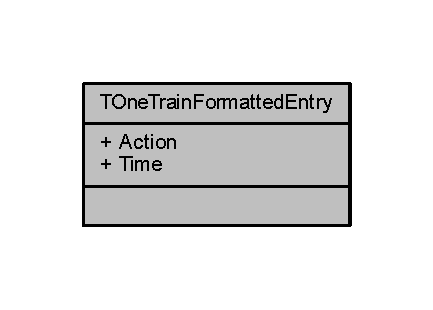
\includegraphics[width=208pt]{class_t_one_train_formatted_entry__coll__graph}
\end{center}
\end{figure}
\subsection*{Public Attributes}
\begin{DoxyCompactItemize}
\item 
\mbox{\Hypertarget{class_t_one_train_formatted_entry_aed96f14cc0862be5da673e206090e6d6}\label{class_t_one_train_formatted_entry_aed96f14cc0862be5da673e206090e6d6}} 
Ansi\+String {\bfseries Action}
\item 
\mbox{\Hypertarget{class_t_one_train_formatted_entry_a1731ee3ca7f8f0a0e7a5d048737bdeec}\label{class_t_one_train_formatted_entry_a1731ee3ca7f8f0a0e7a5d048737bdeec}} 
Ansi\+String {\bfseries Time}
\end{DoxyCompactItemize}


The documentation for this class was generated from the following file\+:\begin{DoxyCompactItemize}
\item 
Train\+Unit.\+h\end{DoxyCompactItemize}

\hypertarget{class_t_pref_dir_element}{}\section{T\+Pref\+Dir\+Element Class Reference}
\label{class_t_pref_dir_element}\index{T\+Pref\+Dir\+Element@{T\+Pref\+Dir\+Element}}


Basic preferred direction or route element -\/ track element with additional members.  




{\ttfamily \#include $<$Track\+Unit.\+h$>$}

Inheritance diagram for T\+Pref\+Dir\+Element\+:\begin{figure}[H]
\begin{center}
\leavevmode
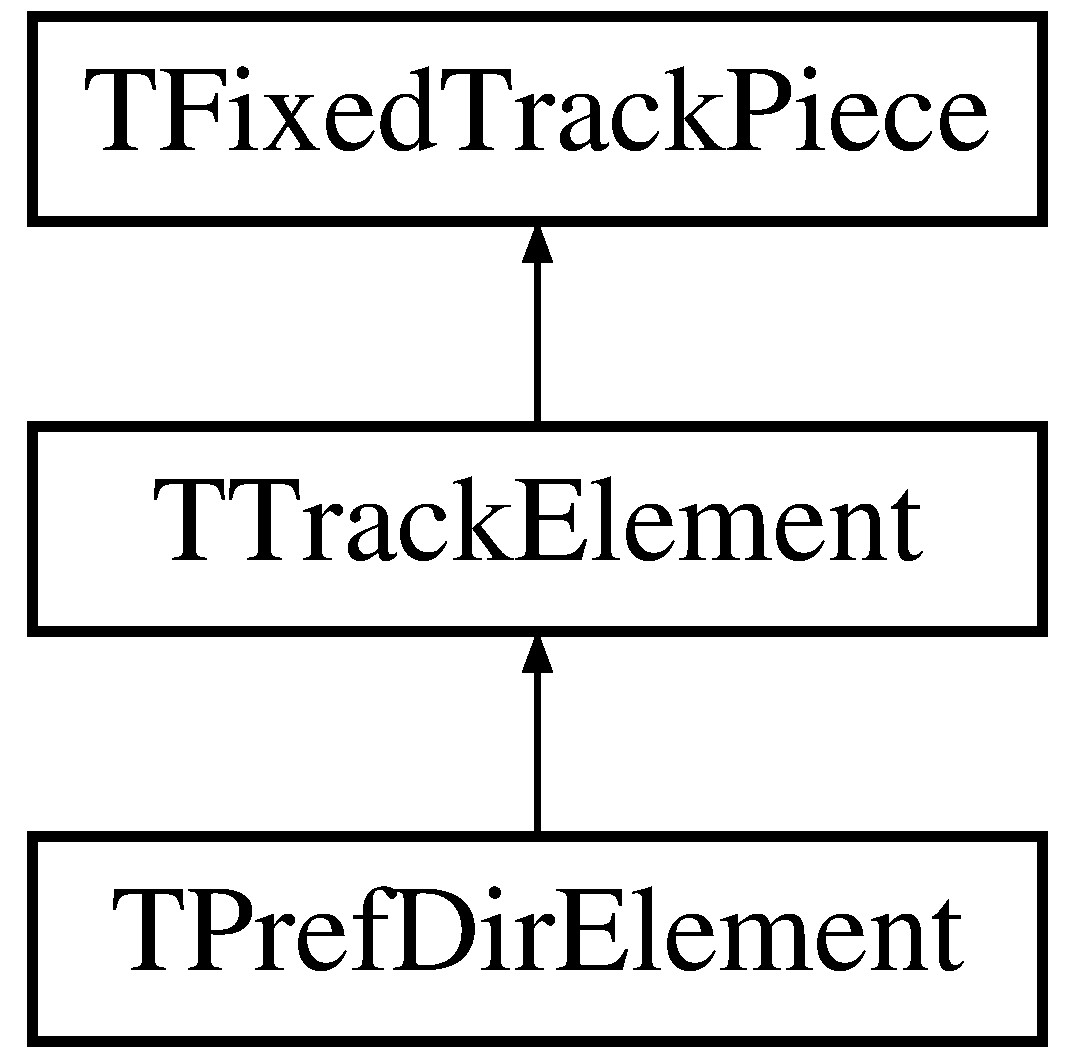
\includegraphics[height=3.000000cm]{class_t_pref_dir_element}
\end{center}
\end{figure}
\subsection*{Public Member Functions}
\begin{DoxyCompactItemize}
\item 
\mbox{\Hypertarget{class_t_pref_dir_element_afa529cc481e34148fd825b49dca7abdd}\label{class_t_pref_dir_element_afa529cc481e34148fd825b49dca7abdd}} 
bool \mbox{\hyperlink{class_t_pref_dir_element_afa529cc481e34148fd825b49dca7abdd}{Is\+Position}} (int Position) const
\begin{DoxyCompactList}\small\item\em Position check. \end{DoxyCompactList}\item 
\mbox{\Hypertarget{class_t_pref_dir_element_af00e0755cd716b4d101abbae02c73ca2}\label{class_t_pref_dir_element_af00e0755cd716b4d101abbae02c73ca2}} 
int \mbox{\hyperlink{class_t_pref_dir_element_af00e0755cd716b4d101abbae02c73ca2}{Get\+E\+Link}} () const
\begin{DoxyCompactList}\small\item\em Returns E\+Link. \end{DoxyCompactList}\item 
\mbox{\Hypertarget{class_t_pref_dir_element_aa5944dedfb065d9e251c26b28fff69f6}\label{class_t_pref_dir_element_aa5944dedfb065d9e251c26b28fff69f6}} 
int \mbox{\hyperlink{class_t_pref_dir_element_aa5944dedfb065d9e251c26b28fff69f6}{Get\+E\+Link\+Pos}} () const
\begin{DoxyCompactList}\small\item\em Returns the E\+Link array position. \end{DoxyCompactList}\item 
\mbox{\Hypertarget{class_t_pref_dir_element_a7c2e4d6a65bce13d02ec469f9ed21b64}\label{class_t_pref_dir_element_a7c2e4d6a65bce13d02ec469f9ed21b64}} 
int \mbox{\hyperlink{class_t_pref_dir_element_a7c2e4d6a65bce13d02ec469f9ed21b64}{Get\+X\+Link}} () const
\begin{DoxyCompactList}\small\item\em Returns X\+Link. \end{DoxyCompactList}\item 
\mbox{\Hypertarget{class_t_pref_dir_element_a35cd9c18012bd537fa988a32c510b01b}\label{class_t_pref_dir_element_a35cd9c18012bd537fa988a32c510b01b}} 
int \mbox{\hyperlink{class_t_pref_dir_element_a35cd9c18012bd537fa988a32c510b01b}{Get\+X\+Link\+Pos}} () const
\begin{DoxyCompactList}\small\item\em Returns the X\+Link array position. \end{DoxyCompactList}\item 
\mbox{\Hypertarget{class_t_pref_dir_element_a0edec31fc9787847e3b6240bab91783c}\label{class_t_pref_dir_element_a0edec31fc9787847e3b6240bab91783c}} 
unsigned int \mbox{\hyperlink{class_t_pref_dir_element_a0edec31fc9787847e3b6240bab91783c}{Get\+Track\+Vector\+Position}} () const
\begin{DoxyCompactList}\small\item\em Returns Track\+Vector\+Position. \end{DoxyCompactList}\item 
\mbox{\Hypertarget{class_t_pref_dir_element_a9fd01c7c6774198d7efe2c9e60ab59bf}\label{class_t_pref_dir_element_a9fd01c7c6774198d7efe2c9e60ab59bf}} 
Graphics\+::\+T\+Bitmap $\ast$ \mbox{\hyperlink{class_t_pref_dir_element_a9fd01c7c6774198d7efe2c9e60ab59bf}{Get\+E\+X\+Graphic\+Ptr}} ()
\begin{DoxyCompactList}\small\item\em Returns E\+X\+Graphic\+Ptr for preferred directions. \end{DoxyCompactList}\item 
\mbox{\Hypertarget{class_t_pref_dir_element_a9dfc04bfa3abf32eb043d771381f971a}\label{class_t_pref_dir_element_a9dfc04bfa3abf32eb043d771381f971a}} 
Graphics\+::\+T\+Bitmap $\ast$ \mbox{\hyperlink{class_t_pref_dir_element_a9dfc04bfa3abf32eb043d771381f971a}{Get\+Route\+E\+X\+Graphic\+Ptr}} ()
\begin{DoxyCompactList}\small\item\em Returns route graphic. \end{DoxyCompactList}\item 
\mbox{\Hypertarget{class_t_pref_dir_element_ab65391b0967a01b2d1b6450ff5ee85a7}\label{class_t_pref_dir_element_ab65391b0967a01b2d1b6450ff5ee85a7}} 
\mbox{\hyperlink{class_t_pref_dir_element_ab65391b0967a01b2d1b6450ff5ee85a7}{T\+Pref\+Dir\+Element}} ()
\begin{DoxyCompactList}\small\item\em Default constructor, loads default values. \end{DoxyCompactList}\item 
\mbox{\hyperlink{class_t_pref_dir_element_a0a06cd720bbc8e23a24d2e3b62f37de5}{T\+Pref\+Dir\+Element}} (\mbox{\hyperlink{class_t_track_element}{T\+Track\+Element}} Input)
\item 
\mbox{\Hypertarget{class_t_pref_dir_element_a473c0faabe4d0fb8c4296c9c70dbe7d3}\label{class_t_pref_dir_element_a473c0faabe4d0fb8c4296c9c70dbe7d3}} 
Ansi\+String \mbox{\hyperlink{class_t_pref_dir_element_a473c0faabe4d0fb8c4296c9c70dbe7d3}{Log\+Pref\+Dir}} () const
\begin{DoxyCompactList}\small\item\em Sends a list of Pref\+Dir\+Element values to Utilities-\/$>$Call\+Log file for debugging purposes. \end{DoxyCompactList}\item 
\mbox{\Hypertarget{class_t_pref_dir_element_a05688db45c02484229e4d226454ed8f3}\label{class_t_pref_dir_element_a05688db45c02484229e4d226454ed8f3}} 
\mbox{\hyperlink{class_t_pref_dir_element_a05688db45c02484229e4d226454ed8f3}{T\+Pref\+Dir\+Element}} (\mbox{\hyperlink{class_t_track_element}{T\+Track\+Element}} Input\+Element, int E\+Link, int \mbox{\hyperlink{class_t_pref_dir_element_a6fc026102a01f722e0e13fdddce13ee0}{E\+Link\+Pos}}, int X\+Link, int \mbox{\hyperlink{class_t_pref_dir_element_aff497780d02596e181f762e55b4423c1}{X\+Link\+Pos}}, int \mbox{\hyperlink{class_t_pref_dir_element_a6b0e69b5e5b4143b9d2c5b0f5c091b64}{Track\+Vector\+Position}})
\begin{DoxyCompactList}\small\item\em Constructs a Pref\+Dir\+Element from supplied values. \end{DoxyCompactList}\end{DoxyCompactItemize}
\subsection*{Public Attributes}
\begin{DoxyCompactItemize}
\item 
\mbox{\Hypertarget{class_t_pref_dir_element_a6aab04763b06d78dfb4e2dc0408fa2e2}\label{class_t_pref_dir_element_a6aab04763b06d78dfb4e2dc0408fa2e2}} 
bool \mbox{\hyperlink{class_t_pref_dir_element_a6aab04763b06d78dfb4e2dc0408fa2e2}{Is\+A\+Route}}
\begin{DoxyCompactList}\small\item\em false for Pref Dir, true for route \end{DoxyCompactList}\item 
\mbox{\Hypertarget{class_t_pref_dir_element_a3d9d35355627dda22fa029dc81fa95c0}\label{class_t_pref_dir_element_a3d9d35355627dda22fa029dc81fa95c0}} 
bool \mbox{\hyperlink{class_t_pref_dir_element_a3d9d35355627dda22fa029dc81fa95c0}{Auto\+Signals}}
\begin{DoxyCompactList}\small\item\em marker within the route for an Auto\+Signal route element \end{DoxyCompactList}\item 
\mbox{\Hypertarget{class_t_pref_dir_element_a96013ae599fd950932832937cada3b96}\label{class_t_pref_dir_element_a96013ae599fd950932832937cada3b96}} 
bool \mbox{\hyperlink{class_t_pref_dir_element_a96013ae599fd950932832937cada3b96}{Consec\+Signals}}
\begin{DoxyCompactList}\small\item\em marker within the route for Consec\+Signals\+Route element \end{DoxyCompactList}\end{DoxyCompactItemize}
\subsection*{Protected Member Functions}
\begin{DoxyCompactItemize}
\item 
\mbox{\Hypertarget{class_t_pref_dir_element_a2f8b222ba3f5990c095d5a4e120681c1}\label{class_t_pref_dir_element_a2f8b222ba3f5990c095d5a4e120681c1}} 
bool \mbox{\hyperlink{class_t_pref_dir_element_a2f8b222ba3f5990c095d5a4e120681c1}{operator==}} (\mbox{\hyperlink{class_t_pref_dir_element}{T\+Pref\+Dir\+Element}} R\+H\+Element)
\begin{DoxyCompactList}\small\item\em equivalence operator \end{DoxyCompactList}\item 
\mbox{\Hypertarget{class_t_pref_dir_element_a22ed5d6b16c6b53f7c3229231791d35e}\label{class_t_pref_dir_element_a22ed5d6b16c6b53f7c3229231791d35e}} 
bool \mbox{\hyperlink{class_t_pref_dir_element_a22ed5d6b16c6b53f7c3229231791d35e}{operator!=}} (\mbox{\hyperlink{class_t_pref_dir_element}{T\+Pref\+Dir\+Element}} R\+H\+Element)
\begin{DoxyCompactList}\small\item\em non-\/equivalence operator \end{DoxyCompactList}\item 
\mbox{\Hypertarget{class_t_pref_dir_element_ae8ee9f59578f80d23aebfdb9fff041d4}\label{class_t_pref_dir_element_ae8ee9f59578f80d23aebfdb9fff041d4}} 
bool \mbox{\hyperlink{class_t_pref_dir_element_ae8ee9f59578f80d23aebfdb9fff041d4}{Entry\+Exit\+Number}} ()
\begin{DoxyCompactList}\small\item\em determines and loads E\+X\+Number (see above) \end{DoxyCompactList}\item 
\mbox{\Hypertarget{class_t_pref_dir_element_a13526cb4ee94a708a7bfef517abaa605}\label{class_t_pref_dir_element_a13526cb4ee94a708a7bfef517abaa605}} 
Graphics\+::\+T\+Bitmap $\ast$ \mbox{\hyperlink{class_t_pref_dir_element_a13526cb4ee94a708a7bfef517abaa605}{Get\+Direction\+Pref\+Dir\+Graphic\+Ptr}} () const
\begin{DoxyCompactList}\small\item\em picks up the Entry\+Direction\+Graphic\+Ptr for preferred directions \end{DoxyCompactList}\item 
Graphics\+::\+T\+Bitmap $\ast$ \mbox{\hyperlink{class_t_pref_dir_element_a5d03028241e6c38e473882120d5bcc68}{Get\+Direction\+Route\+Graphic\+Ptr}} (bool Auto\+Sigs\+Flag, bool Consec\+Signals\+Route) const
\item 
\mbox{\Hypertarget{class_t_pref_dir_element_a9181d9e11c34c6660c43fe2cf4ee35a8}\label{class_t_pref_dir_element_a9181d9e11c34c6660c43fe2cf4ee35a8}} 
Graphics\+::\+T\+Bitmap $\ast$ \mbox{\hyperlink{class_t_pref_dir_element_a9181d9e11c34c6660c43fe2cf4ee35a8}{Get\+Original\+Graphic\+Ptr}} ()
\begin{DoxyCompactList}\small\item\em picks up the original (non-\/flashing) graphic for use during route flashing \end{DoxyCompactList}\item 
\mbox{\Hypertarget{class_t_pref_dir_element_a10b4ff375e779de7cc2a16344959bb31}\label{class_t_pref_dir_element_a10b4ff375e779de7cc2a16344959bb31}} 
Graphics\+::\+T\+Bitmap $\ast$ \mbox{\hyperlink{class_t_pref_dir_element_a10b4ff375e779de7cc2a16344959bb31}{Get\+Pref\+Dir\+Graphic\+Ptr}} ()
\begin{DoxyCompactList}\small\item\em picks up the E\+X\+Graphic\+Ptr for preferred directions \end{DoxyCompactList}\item 
\mbox{\Hypertarget{class_t_pref_dir_element_aee43c641cd4a0550b55105a08ba2cef2}\label{class_t_pref_dir_element_aee43c641cd4a0550b55105a08ba2cef2}} 
Graphics\+::\+T\+Bitmap $\ast$ \mbox{\hyperlink{class_t_pref_dir_element_aee43c641cd4a0550b55105a08ba2cef2}{Get\+Route\+Auto\+Sigs\+Graphic\+Ptr}} ()
\begin{DoxyCompactList}\small\item\em picks up the blue route graphic (not used -\/ superseded by Get\+Route\+Graphic\+Ptr) \end{DoxyCompactList}\item 
\mbox{\Hypertarget{class_t_pref_dir_element_ad58c8d4fa30c04fa9d8e84ae55c7ce61}\label{class_t_pref_dir_element_ad58c8d4fa30c04fa9d8e84ae55c7ce61}} 
Graphics\+::\+T\+Bitmap $\ast$ \mbox{\hyperlink{class_t_pref_dir_element_ad58c8d4fa30c04fa9d8e84ae55c7ce61}{Get\+Route\+Graphic\+Ptr}} (bool Auto\+Sigs\+Flag, bool Consec\+Signals\+Route)
\begin{DoxyCompactList}\small\item\em picks up the appropriate route graphic \end{DoxyCompactList}\end{DoxyCompactItemize}
\subsection*{Protected Attributes}
\begin{DoxyCompactItemize}
\item 
\mbox{\Hypertarget{class_t_pref_dir_element_a7fee253f27bc8cabd8a45d4dcc40a5eb}\label{class_t_pref_dir_element_a7fee253f27bc8cabd8a45d4dcc40a5eb}} 
int {\bfseries E\+Link}
\item 
\mbox{\Hypertarget{class_t_pref_dir_element_a6fc026102a01f722e0e13fdddce13ee0}\label{class_t_pref_dir_element_a6fc026102a01f722e0e13fdddce13ee0}} 
int \mbox{\hyperlink{class_t_pref_dir_element_a6fc026102a01f722e0e13fdddce13ee0}{E\+Link\+Pos}}
\begin{DoxyCompactList}\small\item\em entry link number \& array position \end{DoxyCompactList}\item 
\mbox{\Hypertarget{class_t_pref_dir_element_a8650d58fb9ef3c94bf3f3ca6cc8f6f03}\label{class_t_pref_dir_element_a8650d58fb9ef3c94bf3f3ca6cc8f6f03}} 
int {\bfseries X\+Link}
\item 
\mbox{\Hypertarget{class_t_pref_dir_element_aff497780d02596e181f762e55b4423c1}\label{class_t_pref_dir_element_aff497780d02596e181f762e55b4423c1}} 
int \mbox{\hyperlink{class_t_pref_dir_element_aff497780d02596e181f762e55b4423c1}{X\+Link\+Pos}}
\begin{DoxyCompactList}\small\item\em exit link number \& array position \end{DoxyCompactList}\item 
\mbox{\Hypertarget{class_t_pref_dir_element_a1e631f79e44bdff2d5022349717c0592}\label{class_t_pref_dir_element_a1e631f79e44bdff2d5022349717c0592}} 
int \mbox{\hyperlink{class_t_pref_dir_element_a1e631f79e44bdff2d5022349717c0592}{E\+X\+Number}}
\begin{DoxyCompactList}\small\item\em used to facilitate identification of the appropriate preferred direction or route graphic \end{DoxyCompactList}\item 
\mbox{\Hypertarget{class_t_pref_dir_element_a6b0e69b5e5b4143b9d2c5b0f5c091b64}\label{class_t_pref_dir_element_a6b0e69b5e5b4143b9d2c5b0f5c091b64}} 
int \mbox{\hyperlink{class_t_pref_dir_element_a6b0e69b5e5b4143b9d2c5b0f5c091b64}{Track\+Vector\+Position}}
\begin{DoxyCompactList}\small\item\em Track\+Vector\+Position of the corresponding track element. \end{DoxyCompactList}\item 
\mbox{\Hypertarget{class_t_pref_dir_element_aa6061a11fdf8dab01fe05febc8315707}\label{class_t_pref_dir_element_aa6061a11fdf8dab01fe05febc8315707}} 
int \mbox{\hyperlink{class_t_pref_dir_element_aa6061a11fdf8dab01fe05febc8315707}{Check\+Count}}
\begin{DoxyCompactList}\small\item\em internal check value used when building preferred directions \end{DoxyCompactList}\item 
\mbox{\Hypertarget{class_t_pref_dir_element_ab321e3e65eb5fd3f65d247dc551c535b}\label{class_t_pref_dir_element_ab321e3e65eb5fd3f65d247dc551c535b}} 
Graphics\+::\+T\+Bitmap $\ast$ {\bfseries E\+X\+Graphic\+Ptr}
\item 
Graphics\+::\+T\+Bitmap $\ast$ \mbox{\hyperlink{class_t_pref_dir_element_a523e6fa892a5a25bda21436c23de6732}{Entry\+Direction\+Graphic\+Ptr}}
\end{DoxyCompactItemize}
\subsection*{Friends}
\begin{DoxyCompactItemize}
\item 
\mbox{\Hypertarget{class_t_pref_dir_element_afdf92e6cc78ecd11a5dbdbee36cf58f2}\label{class_t_pref_dir_element_afdf92e6cc78ecd11a5dbdbee36cf58f2}} 
class {\bfseries T\+One\+Pref\+Dir}
\item 
\mbox{\Hypertarget{class_t_pref_dir_element_ac066839379327510645d63c522dbe479}\label{class_t_pref_dir_element_ac066839379327510645d63c522dbe479}} 
class {\bfseries T\+One\+Route}
\item 
\mbox{\Hypertarget{class_t_pref_dir_element_a1496675d125913310dc5b84b640a523d}\label{class_t_pref_dir_element_a1496675d125913310dc5b84b640a523d}} 
class {\bfseries T\+All\+Routes}
\end{DoxyCompactItemize}
\subsection*{Additional Inherited Members}


\subsection{Detailed Description}
Basic preferred direction or route element -\/ track element with additional members. 

\subsection{Constructor \& Destructor Documentation}
\mbox{\Hypertarget{class_t_pref_dir_element_a0a06cd720bbc8e23a24d2e3b62f37de5}\label{class_t_pref_dir_element_a0a06cd720bbc8e23a24d2e3b62f37de5}} 
\index{T\+Pref\+Dir\+Element@{T\+Pref\+Dir\+Element}!T\+Pref\+Dir\+Element@{T\+Pref\+Dir\+Element}}
\index{T\+Pref\+Dir\+Element@{T\+Pref\+Dir\+Element}!T\+Pref\+Dir\+Element@{T\+Pref\+Dir\+Element}}
\subsubsection{\texorpdfstring{T\+Pref\+Dir\+Element()}{TPrefDirElement()}}
{\footnotesize\ttfamily T\+Pref\+Dir\+Element\+::\+T\+Pref\+Dir\+Element (\begin{DoxyParamCaption}\item[{\mbox{\hyperlink{class_t_track_element}{T\+Track\+Element}}}]{Input }\end{DoxyParamCaption})\hspace{0.3cm}{\ttfamily [inline]}}

Constructs a Pref\+Dir\+Element from a base Track\+Element

Sets up the Track\+Element values but leaves others as default values 

\subsection{Member Function Documentation}
\mbox{\Hypertarget{class_t_pref_dir_element_a5d03028241e6c38e473882120d5bcc68}\label{class_t_pref_dir_element_a5d03028241e6c38e473882120d5bcc68}} 
\index{T\+Pref\+Dir\+Element@{T\+Pref\+Dir\+Element}!Get\+Direction\+Route\+Graphic\+Ptr@{Get\+Direction\+Route\+Graphic\+Ptr}}
\index{Get\+Direction\+Route\+Graphic\+Ptr@{Get\+Direction\+Route\+Graphic\+Ptr}!T\+Pref\+Dir\+Element@{T\+Pref\+Dir\+Element}}
\subsubsection{\texorpdfstring{Get\+Direction\+Route\+Graphic\+Ptr()}{GetDirectionRouteGraphicPtr()}}
{\footnotesize\ttfamily Graphics\+::\+T\+Bitmap $\ast$ T\+Pref\+Dir\+Element\+::\+Get\+Direction\+Route\+Graphic\+Ptr (\begin{DoxyParamCaption}\item[{bool}]{Auto\+Sigs\+Flag,  }\item[{bool}]{Consec\+Signals\+Route }\end{DoxyParamCaption}) const\hspace{0.3cm}{\ttfamily [protected]}}

picks up the green or red route direction graphic 

\subsection{Member Data Documentation}
\mbox{\Hypertarget{class_t_pref_dir_element_a523e6fa892a5a25bda21436c23de6732}\label{class_t_pref_dir_element_a523e6fa892a5a25bda21436c23de6732}} 
\index{T\+Pref\+Dir\+Element@{T\+Pref\+Dir\+Element}!Entry\+Direction\+Graphic\+Ptr@{Entry\+Direction\+Graphic\+Ptr}}
\index{Entry\+Direction\+Graphic\+Ptr@{Entry\+Direction\+Graphic\+Ptr}!T\+Pref\+Dir\+Element@{T\+Pref\+Dir\+Element}}
\subsubsection{\texorpdfstring{Entry\+Direction\+Graphic\+Ptr}{EntryDirectionGraphicPtr}}
{\footnotesize\ttfamily Graphics\+::\+T\+Bitmap $\ast$ T\+Pref\+Dir\+Element\+::\+Entry\+Direction\+Graphic\+Ptr\hspace{0.3cm}{\ttfamily [protected]}}

pointers to the appropriate entry/exit graphic, or direction marker graphic, for preferred directions and routes 

The documentation for this class was generated from the following files\+:\begin{DoxyCompactItemize}
\item 
Track\+Unit.\+h\item 
Track\+Unit.\+cpp\end{DoxyCompactItemize}

\hypertarget{class_t_rail_graphics}{}\section{T\+Rail\+Graphics Class Reference}
\label{class_t_rail_graphics}\index{T\+Rail\+Graphics@{T\+Rail\+Graphics}}


Handles graphic data \& functions, single object defined.  




{\ttfamily \#include $<$Graphic\+Unit.\+h$>$}



Collaboration diagram for T\+Rail\+Graphics\+:\nopagebreak
\begin{figure}[H]
\begin{center}
\leavevmode
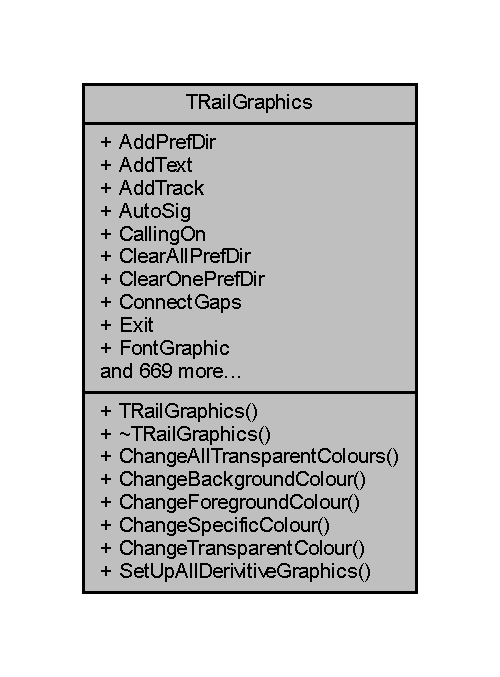
\includegraphics[width=240pt]{class_t_rail_graphics__coll__graph}
\end{center}
\end{figure}
\subsection*{Public Member Functions}
\begin{DoxyCompactItemize}
\item 
\mbox{\Hypertarget{class_t_rail_graphics_acd3dfcf9686870772b1708030f11b1d4}\label{class_t_rail_graphics_acd3dfcf9686870772b1708030f11b1d4}} 
\mbox{\hyperlink{class_t_rail_graphics_acd3dfcf9686870772b1708030f11b1d4}{T\+Rail\+Graphics}} ()
\begin{DoxyCompactList}\small\item\em constructor \end{DoxyCompactList}\item 
\mbox{\hyperlink{class_t_rail_graphics_ad243415e657236ecca97fa1d064cf127}{$\sim$\+T\+Rail\+Graphics}} ()
\item 
void \mbox{\hyperlink{class_t_rail_graphics_a5121c6d8b8fa69eefc293ca51cddce88}{Change\+All\+Transparent\+Colours}} (T\+Color New\+Transparent\+Colour, T\+Color Old\+Transparent\+Colour)
\item 
void \mbox{\hyperlink{class_t_rail_graphics_a74d7dcd5e17ef156d8c216c8e524de11}{Change\+Background\+Colour}} (int Caller, Graphics\+::\+T\+Bitmap $\ast$Bitmap\+In, Graphics\+::\+T\+Bitmap $\ast$Bitmap\+Out, T\+Color New\+Background\+Colour, T\+Color Old\+Background\+Colour, bool \&Colour\+Error)
\item 
void \mbox{\hyperlink{class_t_rail_graphics_aa2dace651659e084ec23c9961f5819b1}{Change\+Foreground\+Colour}} (int Caller, Graphics\+::\+T\+Bitmap $\ast$Bitmap\+In, Graphics\+::\+T\+Bitmap $\ast$Bitmap\+Out, T\+Color New\+Foreground\+Colour, T\+Color Background\+Colour)
\item 
void \mbox{\hyperlink{class_t_rail_graphics_ac4e48e6ee19e01724adb0d490762d548}{Change\+Specific\+Colour}} (int Caller, Graphics\+::\+T\+Bitmap $\ast$Bitmap\+In, Graphics\+::\+T\+Bitmap $\ast$Bitmap\+Out, T\+Color Colour\+To\+Be\+Changed, T\+Color New\+Colour)
\item 
void \mbox{\hyperlink{class_t_rail_graphics_a89a3e3a91129c4d02f4606478781b519}{Change\+Transparent\+Colour}} (Graphics\+::\+T\+Bitmap $\ast$Bitmap\+In, Graphics\+::\+T\+Bitmap $\ast$Bitmap\+Out, T\+Color New\+Transparent\+Colour, T\+Color Old\+Transparent\+Colour)
\item 
void \mbox{\hyperlink{class_t_rail_graphics_ae19696d461eea07c5444ed4c9714acf3}{Set\+Up\+All\+Derivitive\+Graphics}} (T\+Color Transparent\+Colour)
\end{DoxyCompactItemize}
\subsection*{Public Attributes}
\begin{DoxyCompactItemize}
\item 
\mbox{\Hypertarget{class_t_rail_graphics_a7c4b141ce406b2cdfe884579cb442480}\label{class_t_rail_graphics_a7c4b141ce406b2cdfe884579cb442480}} 
Graphics\+::\+T\+Bitmap $\ast$ {\bfseries Add\+Pref\+Dir}
\item 
\mbox{\Hypertarget{class_t_rail_graphics_ac4cacf43258ed3732a278a8f6ba2aa51}\label{class_t_rail_graphics_ac4cacf43258ed3732a278a8f6ba2aa51}} 
Graphics\+::\+T\+Bitmap $\ast$ {\bfseries Add\+Text}
\item 
\mbox{\Hypertarget{class_t_rail_graphics_a68377a08393996c533d2b841adce49e7}\label{class_t_rail_graphics_a68377a08393996c533d2b841adce49e7}} 
Graphics\+::\+T\+Bitmap $\ast$ {\bfseries Add\+Track}
\item 
\mbox{\Hypertarget{class_t_rail_graphics_a3cb0db29cb0fb6cb7258d6a48b78bc0c}\label{class_t_rail_graphics_a3cb0db29cb0fb6cb7258d6a48b78bc0c}} 
Graphics\+::\+T\+Bitmap $\ast$ {\bfseries Auto\+Sig}
\item 
\mbox{\Hypertarget{class_t_rail_graphics_aae89b69c01237c9719e8018983632dca}\label{class_t_rail_graphics_aae89b69c01237c9719e8018983632dca}} 
Graphics\+::\+T\+Bitmap $\ast$ {\bfseries Calling\+On}
\item 
\mbox{\Hypertarget{class_t_rail_graphics_a97503c28ed454585384bd0fd08017c6d}\label{class_t_rail_graphics_a97503c28ed454585384bd0fd08017c6d}} 
Graphics\+::\+T\+Bitmap $\ast$ {\bfseries Clear\+All\+Pref\+Dir}
\item 
\mbox{\Hypertarget{class_t_rail_graphics_a5cd913f6afb418df4c2bce19a8d05c11}\label{class_t_rail_graphics_a5cd913f6afb418df4c2bce19a8d05c11}} 
Graphics\+::\+T\+Bitmap $\ast$ {\bfseries Clear\+One\+Pref\+Dir}
\item 
\mbox{\Hypertarget{class_t_rail_graphics_a1182337fbbfff6fb51b224a9fc3140cf}\label{class_t_rail_graphics_a1182337fbbfff6fb51b224a9fc3140cf}} 
Graphics\+::\+T\+Bitmap $\ast$ {\bfseries Connect\+Gaps}
\item 
\mbox{\Hypertarget{class_t_rail_graphics_a982b81e96ff8250ef27b0f4bc23b1e82}\label{class_t_rail_graphics_a982b81e96ff8250ef27b0f4bc23b1e82}} 
Graphics\+::\+T\+Bitmap $\ast$ {\bfseries Exit}
\item 
\mbox{\Hypertarget{class_t_rail_graphics_ab6b49973b1db415846e1b1904c92ca0f}\label{class_t_rail_graphics_ab6b49973b1db415846e1b1904c92ca0f}} 
Graphics\+::\+T\+Bitmap $\ast$ {\bfseries Font\+Graphic}
\item 
\mbox{\Hypertarget{class_t_rail_graphics_ad702ccce1f5a5beb24d1a1161027f3b9}\label{class_t_rail_graphics_ad702ccce1f5a5beb24d1a1161027f3b9}} 
Graphics\+::\+T\+Bitmap $\ast$ {\bfseries Hide}
\item 
\mbox{\Hypertarget{class_t_rail_graphics_af0646f6c9d448bc7f6f133f69a0b651f}\label{class_t_rail_graphics_af0646f6c9d448bc7f6f133f69a0b651f}} 
Graphics\+::\+T\+Bitmap $\ast$ {\bfseries Move\+Text}
\item 
\mbox{\Hypertarget{class_t_rail_graphics_a653a0e9052ed4d979bb994821911980b}\label{class_t_rail_graphics_a653a0e9052ed4d979bb994821911980b}} 
Graphics\+::\+T\+Bitmap $\ast$ {\bfseries Name\+Locs}
\item 
\mbox{\Hypertarget{class_t_rail_graphics_ab9c824df118929808afd6892475942e8}\label{class_t_rail_graphics_ab9c824df118929808afd6892475942e8}} 
Graphics\+::\+T\+Bitmap $\ast$ {\bfseries Non\+Sig}
\item 
\mbox{\Hypertarget{class_t_rail_graphics_a5ac4abd11a49b04e57bb168a17739657}\label{class_t_rail_graphics_a5ac4abd11a49b04e57bb168a17739657}} 
Graphics\+::\+T\+Bitmap $\ast$ {\bfseries Pref\+Sig}
\item 
\mbox{\Hypertarget{class_t_rail_graphics_a778d7e836f4882b62ffec464a6e52916}\label{class_t_rail_graphics_a778d7e836f4882b62ffec464a6e52916}} 
Graphics\+::\+T\+Bitmap $\ast$ {\bfseries Route\+Cancel}
\item 
\mbox{\Hypertarget{class_t_rail_graphics_ad892b2631bf51a1e780109d2dd59bb75}\label{class_t_rail_graphics_ad892b2631bf51a1e780109d2dd59bb75}} 
Graphics\+::\+T\+Bitmap $\ast$ {\bfseries Save\+Railway}
\item 
\mbox{\Hypertarget{class_t_rail_graphics_a49078dde6b77e13b80cabda92d5c3b30}\label{class_t_rail_graphics_a49078dde6b77e13b80cabda92d5c3b30}} 
Graphics\+::\+T\+Bitmap $\ast$ {\bfseries Save\+Session}
\item 
\mbox{\Hypertarget{class_t_rail_graphics_abe3a2be9670be112baaaa9888ca437ac}\label{class_t_rail_graphics_abe3a2be9670be112baaaa9888ca437ac}} 
Graphics\+::\+T\+Bitmap $\ast$ {\bfseries Screen\+Grid}
\item 
\mbox{\Hypertarget{class_t_rail_graphics_aeba701e6a6ce2c0de840cb68824f7200}\label{class_t_rail_graphics_aeba701e6a6ce2c0de840cb68824f7200}} 
Graphics\+::\+T\+Bitmap $\ast$ {\bfseries Set\+Dists}
\item 
\mbox{\Hypertarget{class_t_rail_graphics_a44047d6244ef830fcc00c9f326b79d47}\label{class_t_rail_graphics_a44047d6244ef830fcc00c9f326b79d47}} 
Graphics\+::\+T\+Bitmap $\ast$ {\bfseries Show}
\item 
\mbox{\Hypertarget{class_t_rail_graphics_ae9a78e64d31b6cf35403f1c2937abd9d}\label{class_t_rail_graphics_ae9a78e64d31b6cf35403f1c2937abd9d}} 
Graphics\+::\+T\+Bitmap $\ast$ {\bfseries Validate}
\item 
\mbox{\Hypertarget{class_t_rail_graphics_af48ccc801c7143f747aba327a7869320}\label{class_t_rail_graphics_af48ccc801c7143f747aba327a7869320}} 
Graphics\+::\+T\+Bitmap $\ast$ {\bfseries Distance\+Key}
\item 
\mbox{\Hypertarget{class_t_rail_graphics_a0e08cf7b116c4c545139dfe418296338}\label{class_t_rail_graphics_a0e08cf7b116c4c545139dfe418296338}} 
Graphics\+::\+T\+Bitmap $\ast$ {\bfseries Pref\+Dir\+Key}
\item 
\mbox{\Hypertarget{class_t_rail_graphics_ab4266639a3d1fae17706c782d4f872b5}\label{class_t_rail_graphics_ab4266639a3d1fae17706c782d4f872b5}} 
Graphics\+::\+T\+Bitmap $\ast$ {\bfseries Buffer\+Warning}
\item 
\mbox{\Hypertarget{class_t_rail_graphics_ac81b876f0a341f6a5ed1185604548843}\label{class_t_rail_graphics_ac81b876f0a341f6a5ed1185604548843}} 
Graphics\+::\+T\+Bitmap $\ast$ {\bfseries Crash\+Warning}
\item 
\mbox{\Hypertarget{class_t_rail_graphics_a2c688dc7a18b9121fd6c394c2564eac6}\label{class_t_rail_graphics_a2c688dc7a18b9121fd6c394c2564eac6}} 
Graphics\+::\+T\+Bitmap $\ast$ {\bfseries Derail\+Warning}
\item 
\mbox{\Hypertarget{class_t_rail_graphics_ab5e0043589fd2170e5197d1155feded0}\label{class_t_rail_graphics_ab5e0043589fd2170e5197d1155feded0}} 
Graphics\+::\+T\+Bitmap $\ast$ {\bfseries Signal\+Stop\+Warning}
\item 
\mbox{\Hypertarget{class_t_rail_graphics_a203aeac4b19334e66045842d01d96c01}\label{class_t_rail_graphics_a203aeac4b19334e66045842d01d96c01}} 
Graphics\+::\+T\+Bitmap $\ast$ {\bfseries S\+P\+A\+D\+Warning}
\item 
\mbox{\Hypertarget{class_t_rail_graphics_adf4324337b8b51dd5152bb5d9c325eaa}\label{class_t_rail_graphics_adf4324337b8b51dd5152bb5d9c325eaa}} 
Graphics\+::\+T\+Bitmap $\ast$ {\bfseries Black\+Arrow\+Down}
\item 
\mbox{\Hypertarget{class_t_rail_graphics_a901c5a179049ea0770d30361b6d3310d}\label{class_t_rail_graphics_a901c5a179049ea0770d30361b6d3310d}} 
Graphics\+::\+T\+Bitmap $\ast$ {\bfseries Black\+Arrow\+Left}
\item 
\mbox{\Hypertarget{class_t_rail_graphics_a5fee8108951d2432251dcae065ce5f9b}\label{class_t_rail_graphics_a5fee8108951d2432251dcae065ce5f9b}} 
Graphics\+::\+T\+Bitmap $\ast$ {\bfseries Black\+Arrow\+Right}
\item 
\mbox{\Hypertarget{class_t_rail_graphics_aa3eefa8b7a6c057cd86a561400164436}\label{class_t_rail_graphics_aa3eefa8b7a6c057cd86a561400164436}} 
Graphics\+::\+T\+Bitmap $\ast$ {\bfseries Black\+Arrow\+Up}
\item 
\mbox{\Hypertarget{class_t_rail_graphics_ac90712563e9782c14c0bd7e2755d2f3a}\label{class_t_rail_graphics_ac90712563e9782c14c0bd7e2755d2f3a}} 
Graphics\+::\+T\+Bitmap $\ast$ {\bfseries bm10}
\item 
\mbox{\Hypertarget{class_t_rail_graphics_a7c0bc75bfc80599eae290b56f4a7fc26}\label{class_t_rail_graphics_a7c0bc75bfc80599eae290b56f4a7fc26}} 
Graphics\+::\+T\+Bitmap $\ast$ {\bfseries bm100}
\item 
\mbox{\Hypertarget{class_t_rail_graphics_a8967ef33374406c1aea4040af662bf6b}\label{class_t_rail_graphics_a8967ef33374406c1aea4040af662bf6b}} 
Graphics\+::\+T\+Bitmap $\ast$ {\bfseries bm101}
\item 
\mbox{\Hypertarget{class_t_rail_graphics_a6640af58c140d59f073494aa7a7cfc21}\label{class_t_rail_graphics_a6640af58c140d59f073494aa7a7cfc21}} 
Graphics\+::\+T\+Bitmap $\ast$ {\bfseries bm106}
\item 
\mbox{\Hypertarget{class_t_rail_graphics_a28466edbe03d707fdf440b7e59c4c3d5}\label{class_t_rail_graphics_a28466edbe03d707fdf440b7e59c4c3d5}} 
Graphics\+::\+T\+Bitmap $\ast$ {\bfseries bm10\+Diverging}
\item 
\mbox{\Hypertarget{class_t_rail_graphics_a53df65487a010456be69d6fcc61cf2ea}\label{class_t_rail_graphics_a53df65487a010456be69d6fcc61cf2ea}} 
Graphics\+::\+T\+Bitmap $\ast$ {\bfseries bm10\+Straight}
\item 
\mbox{\Hypertarget{class_t_rail_graphics_a6a6da0748b5d0e46eaa82223ad9ce348}\label{class_t_rail_graphics_a6a6da0748b5d0e46eaa82223ad9ce348}} 
Graphics\+::\+T\+Bitmap $\ast$ {\bfseries bm11}
\item 
\mbox{\Hypertarget{class_t_rail_graphics_aa0f7e0055c2d4ee325a4304f4e097875}\label{class_t_rail_graphics_aa0f7e0055c2d4ee325a4304f4e097875}} 
Graphics\+::\+T\+Bitmap $\ast$ {\bfseries bm11\+Diverging}
\item 
\mbox{\Hypertarget{class_t_rail_graphics_aa019677e2893e62a46b160a045cc8965}\label{class_t_rail_graphics_aa019677e2893e62a46b160a045cc8965}} 
Graphics\+::\+T\+Bitmap $\ast$ {\bfseries bm11\+Straight}
\item 
\mbox{\Hypertarget{class_t_rail_graphics_a52a527d3cb0e6ed788c2af35595132a0}\label{class_t_rail_graphics_a52a527d3cb0e6ed788c2af35595132a0}} 
Graphics\+::\+T\+Bitmap $\ast$ {\bfseries bm12}
\item 
\mbox{\Hypertarget{class_t_rail_graphics_a17c77fd048778136a897152a0f700608}\label{class_t_rail_graphics_a17c77fd048778136a897152a0f700608}} 
Graphics\+::\+T\+Bitmap $\ast$ {\bfseries bm12\+Diverging}
\item 
\mbox{\Hypertarget{class_t_rail_graphics_a77716be550bb4be608ff458671e085fe}\label{class_t_rail_graphics_a77716be550bb4be608ff458671e085fe}} 
Graphics\+::\+T\+Bitmap $\ast$ {\bfseries bm12\+Straight}
\item 
\mbox{\Hypertarget{class_t_rail_graphics_a20c24eede5487acbf8499f056c13e41d}\label{class_t_rail_graphics_a20c24eede5487acbf8499f056c13e41d}} 
Graphics\+::\+T\+Bitmap $\ast$ {\bfseries bm13}
\item 
\mbox{\Hypertarget{class_t_rail_graphics_ae8ebfc7306f6e1313aad3a097e241970}\label{class_t_rail_graphics_ae8ebfc7306f6e1313aad3a097e241970}} 
Graphics\+::\+T\+Bitmap $\ast$ {\bfseries bm132}
\item 
\mbox{\Hypertarget{class_t_rail_graphics_af662d45855f58077ce874d6bed5585c6}\label{class_t_rail_graphics_af662d45855f58077ce874d6bed5585c6}} 
Graphics\+::\+T\+Bitmap $\ast$ {\bfseries bm132\+Left\+Fork}
\item 
\mbox{\Hypertarget{class_t_rail_graphics_ab1edb1d0f80aebbe57044c78c2b631d0}\label{class_t_rail_graphics_ab1edb1d0f80aebbe57044c78c2b631d0}} 
Graphics\+::\+T\+Bitmap $\ast$ {\bfseries bm132\+Right\+Fork}
\item 
\mbox{\Hypertarget{class_t_rail_graphics_a4e622deb7fdcbd6087df9c8f16de875a}\label{class_t_rail_graphics_a4e622deb7fdcbd6087df9c8f16de875a}} 
Graphics\+::\+T\+Bitmap $\ast$ {\bfseries bm133}
\item 
\mbox{\Hypertarget{class_t_rail_graphics_a037fa3e16084e50d1791d88a291b1f27}\label{class_t_rail_graphics_a037fa3e16084e50d1791d88a291b1f27}} 
Graphics\+::\+T\+Bitmap $\ast$ {\bfseries bm133\+Left\+Fork}
\item 
\mbox{\Hypertarget{class_t_rail_graphics_a87689b93979a91d618b0b4f41ca1af85}\label{class_t_rail_graphics_a87689b93979a91d618b0b4f41ca1af85}} 
Graphics\+::\+T\+Bitmap $\ast$ {\bfseries bm133\+Right\+Fork}
\item 
\mbox{\Hypertarget{class_t_rail_graphics_af9864e15787535b5e5f67b6858462c51}\label{class_t_rail_graphics_af9864e15787535b5e5f67b6858462c51}} 
Graphics\+::\+T\+Bitmap $\ast$ {\bfseries bm134}
\item 
\mbox{\Hypertarget{class_t_rail_graphics_ad469c3408c51298e999218ccc30f509a}\label{class_t_rail_graphics_ad469c3408c51298e999218ccc30f509a}} 
Graphics\+::\+T\+Bitmap $\ast$ {\bfseries bm134\+Left\+Fork}
\item 
\mbox{\Hypertarget{class_t_rail_graphics_a274c4bf7b572362caee277c5f4299d09}\label{class_t_rail_graphics_a274c4bf7b572362caee277c5f4299d09}} 
Graphics\+::\+T\+Bitmap $\ast$ {\bfseries bm134\+Right\+Fork}
\item 
\mbox{\Hypertarget{class_t_rail_graphics_a798f44fa5ba583d5206daa604b2edf47}\label{class_t_rail_graphics_a798f44fa5ba583d5206daa604b2edf47}} 
Graphics\+::\+T\+Bitmap $\ast$ {\bfseries bm135}
\item 
\mbox{\Hypertarget{class_t_rail_graphics_ae27a631d37eaef70b4bce78d50e0457d}\label{class_t_rail_graphics_ae27a631d37eaef70b4bce78d50e0457d}} 
Graphics\+::\+T\+Bitmap $\ast$ {\bfseries bm135\+Left\+Fork}
\item 
\mbox{\Hypertarget{class_t_rail_graphics_a48383902d8e00fe170c2748a3a23d13d}\label{class_t_rail_graphics_a48383902d8e00fe170c2748a3a23d13d}} 
Graphics\+::\+T\+Bitmap $\ast$ {\bfseries bm135\+Right\+Fork}
\item 
\mbox{\Hypertarget{class_t_rail_graphics_a2e3c02de58199e0f68b09148dc9a6bb0}\label{class_t_rail_graphics_a2e3c02de58199e0f68b09148dc9a6bb0}} 
Graphics\+::\+T\+Bitmap $\ast$ {\bfseries bm136}
\item 
\mbox{\Hypertarget{class_t_rail_graphics_a8c87e431097f966ff9f4c3249e5e3873}\label{class_t_rail_graphics_a8c87e431097f966ff9f4c3249e5e3873}} 
Graphics\+::\+T\+Bitmap $\ast$ {\bfseries bm136\+Left\+Fork}
\item 
\mbox{\Hypertarget{class_t_rail_graphics_a4ec36ad58e9170013deb45e8ea4ab1a4}\label{class_t_rail_graphics_a4ec36ad58e9170013deb45e8ea4ab1a4}} 
Graphics\+::\+T\+Bitmap $\ast$ {\bfseries bm136\+Right\+Fork}
\item 
\mbox{\Hypertarget{class_t_rail_graphics_aee67a27fa32efa6570c95fe25ce7343c}\label{class_t_rail_graphics_aee67a27fa32efa6570c95fe25ce7343c}} 
Graphics\+::\+T\+Bitmap $\ast$ {\bfseries bm137}
\item 
\mbox{\Hypertarget{class_t_rail_graphics_aba75c89eff41b63648ca91a7155afabc}\label{class_t_rail_graphics_aba75c89eff41b63648ca91a7155afabc}} 
Graphics\+::\+T\+Bitmap $\ast$ {\bfseries bm137\+Left\+Fork}
\item 
\mbox{\Hypertarget{class_t_rail_graphics_ab8e5f851126fe438ec770bb238a339f9}\label{class_t_rail_graphics_ab8e5f851126fe438ec770bb238a339f9}} 
Graphics\+::\+T\+Bitmap $\ast$ {\bfseries bm137\+Right\+Fork}
\item 
\mbox{\Hypertarget{class_t_rail_graphics_a5699103895491170e806d9ddd910b8ae}\label{class_t_rail_graphics_a5699103895491170e806d9ddd910b8ae}} 
Graphics\+::\+T\+Bitmap $\ast$ {\bfseries bm138}
\item 
\mbox{\Hypertarget{class_t_rail_graphics_a058a639cebf05f499662e33c4348e599}\label{class_t_rail_graphics_a058a639cebf05f499662e33c4348e599}} 
Graphics\+::\+T\+Bitmap $\ast$ {\bfseries bm138\+Left\+Fork}
\item 
\mbox{\Hypertarget{class_t_rail_graphics_a80a406c8737eaf128d7aa76568969b1c}\label{class_t_rail_graphics_a80a406c8737eaf128d7aa76568969b1c}} 
Graphics\+::\+T\+Bitmap $\ast$ {\bfseries bm138\+Right\+Fork}
\item 
\mbox{\Hypertarget{class_t_rail_graphics_a7373405f1eacf5e76ec85d62ab6b25e1}\label{class_t_rail_graphics_a7373405f1eacf5e76ec85d62ab6b25e1}} 
Graphics\+::\+T\+Bitmap $\ast$ {\bfseries bm139}
\item 
\mbox{\Hypertarget{class_t_rail_graphics_a45157cd244d9ca8e93e2559a0c15e300}\label{class_t_rail_graphics_a45157cd244d9ca8e93e2559a0c15e300}} 
Graphics\+::\+T\+Bitmap $\ast$ {\bfseries bm139\+Left\+Fork}
\item 
\mbox{\Hypertarget{class_t_rail_graphics_aca33c787bc9fa38876f65a746ecc4fee}\label{class_t_rail_graphics_aca33c787bc9fa38876f65a746ecc4fee}} 
Graphics\+::\+T\+Bitmap $\ast$ {\bfseries bm139\+Right\+Fork}
\item 
\mbox{\Hypertarget{class_t_rail_graphics_acbeaa1a097c03e926a7d0673b9b8f79f}\label{class_t_rail_graphics_acbeaa1a097c03e926a7d0673b9b8f79f}} 
Graphics\+::\+T\+Bitmap $\ast$ {\bfseries bm13\+Diverging}
\item 
\mbox{\Hypertarget{class_t_rail_graphics_aa93df944790ca2dde9fd6f460f6084fc}\label{class_t_rail_graphics_aa93df944790ca2dde9fd6f460f6084fc}} 
Graphics\+::\+T\+Bitmap $\ast$ {\bfseries bm13\+Straight}
\item 
\mbox{\Hypertarget{class_t_rail_graphics_aec0cd921ce6d8f8ce7413c361921fc09}\label{class_t_rail_graphics_aec0cd921ce6d8f8ce7413c361921fc09}} 
Graphics\+::\+T\+Bitmap $\ast$ {\bfseries bm14}
\item 
\mbox{\Hypertarget{class_t_rail_graphics_a8ab41b712e4a279e530fbc353c08c5e4}\label{class_t_rail_graphics_a8ab41b712e4a279e530fbc353c08c5e4}} 
Graphics\+::\+T\+Bitmap $\ast$ {\bfseries bm140}
\item 
\mbox{\Hypertarget{class_t_rail_graphics_a810a8b649eb44bfb0ad777fd0347f2cc}\label{class_t_rail_graphics_a810a8b649eb44bfb0ad777fd0347f2cc}} 
Graphics\+::\+T\+Bitmap $\ast$ {\bfseries bm141}
\item 
\mbox{\Hypertarget{class_t_rail_graphics_aab3e9deef527debbd1bec850f3607ff8}\label{class_t_rail_graphics_aab3e9deef527debbd1bec850f3607ff8}} 
Graphics\+::\+T\+Bitmap $\ast$ {\bfseries bm14\+Diverging}
\item 
\mbox{\Hypertarget{class_t_rail_graphics_a79332550ac493d898a47ff87fc05f5a6}\label{class_t_rail_graphics_a79332550ac493d898a47ff87fc05f5a6}} 
Graphics\+::\+T\+Bitmap $\ast$ {\bfseries bm14\+Straight}
\item 
\mbox{\Hypertarget{class_t_rail_graphics_af4d0a9073bbf8e04549050e577bf41f3}\label{class_t_rail_graphics_af4d0a9073bbf8e04549050e577bf41f3}} 
Graphics\+::\+T\+Bitmap $\ast$ {\bfseries bm16}
\item 
\mbox{\Hypertarget{class_t_rail_graphics_a7d3f4e55607012069ba88ea07eb5dd6c}\label{class_t_rail_graphics_a7d3f4e55607012069ba88ea07eb5dd6c}} 
Graphics\+::\+T\+Bitmap $\ast$ {\bfseries bm18}
\item 
\mbox{\Hypertarget{class_t_rail_graphics_acb9390518394a90d1e9d9c18f43eb28b}\label{class_t_rail_graphics_acb9390518394a90d1e9d9c18f43eb28b}} 
Graphics\+::\+T\+Bitmap $\ast$ {\bfseries bm20}
\item 
\mbox{\Hypertarget{class_t_rail_graphics_a85b3ca7d2183d40b5fedbc8bb267f7f5}\label{class_t_rail_graphics_a85b3ca7d2183d40b5fedbc8bb267f7f5}} 
Graphics\+::\+T\+Bitmap $\ast$ {\bfseries bm27}
\item 
\mbox{\Hypertarget{class_t_rail_graphics_a0826647859d8d431761419eddd66c181}\label{class_t_rail_graphics_a0826647859d8d431761419eddd66c181}} 
Graphics\+::\+T\+Bitmap $\ast$ {\bfseries bm28}
\item 
\mbox{\Hypertarget{class_t_rail_graphics_a8839f6eaeb81f375746aec677fdf6ec9}\label{class_t_rail_graphics_a8839f6eaeb81f375746aec677fdf6ec9}} 
Graphics\+::\+T\+Bitmap $\ast$ {\bfseries bm28\+Diverging}
\item 
\mbox{\Hypertarget{class_t_rail_graphics_ac0c824885240eb7d2df26d4c11fe687d}\label{class_t_rail_graphics_ac0c824885240eb7d2df26d4c11fe687d}} 
Graphics\+::\+T\+Bitmap $\ast$ {\bfseries bm28\+Straight}
\item 
\mbox{\Hypertarget{class_t_rail_graphics_a09842177650d3075a6616c60517d82b8}\label{class_t_rail_graphics_a09842177650d3075a6616c60517d82b8}} 
Graphics\+::\+T\+Bitmap $\ast$ {\bfseries bm29}
\item 
\mbox{\Hypertarget{class_t_rail_graphics_a7407fb6411def3f84b06b7df9e8c51eb}\label{class_t_rail_graphics_a7407fb6411def3f84b06b7df9e8c51eb}} 
Graphics\+::\+T\+Bitmap $\ast$ {\bfseries bm29\+Diverging}
\item 
\mbox{\Hypertarget{class_t_rail_graphics_a0dbf2d8f3c3b0484577c243b308c59fb}\label{class_t_rail_graphics_a0dbf2d8f3c3b0484577c243b308c59fb}} 
Graphics\+::\+T\+Bitmap $\ast$ {\bfseries bm29\+Straight}
\item 
\mbox{\Hypertarget{class_t_rail_graphics_a9448043ef27be3886a98753a6c6d8485}\label{class_t_rail_graphics_a9448043ef27be3886a98753a6c6d8485}} 
Graphics\+::\+T\+Bitmap $\ast$ {\bfseries bm30}
\item 
\mbox{\Hypertarget{class_t_rail_graphics_aa86d4ebfafd54ccc7f2d086335922e67}\label{class_t_rail_graphics_aa86d4ebfafd54ccc7f2d086335922e67}} 
Graphics\+::\+T\+Bitmap $\ast$ {\bfseries bm30\+Diverging}
\item 
\mbox{\Hypertarget{class_t_rail_graphics_a0a81febdf64c3936c13d4c8d7691ef20}\label{class_t_rail_graphics_a0a81febdf64c3936c13d4c8d7691ef20}} 
Graphics\+::\+T\+Bitmap $\ast$ {\bfseries bm30\+Straight}
\item 
\mbox{\Hypertarget{class_t_rail_graphics_a578d423f8a1a0c6caad89b118e3d7806}\label{class_t_rail_graphics_a578d423f8a1a0c6caad89b118e3d7806}} 
Graphics\+::\+T\+Bitmap $\ast$ {\bfseries bm31}
\item 
\mbox{\Hypertarget{class_t_rail_graphics_aa6616cad13abf11cceb9081dbe50f147}\label{class_t_rail_graphics_aa6616cad13abf11cceb9081dbe50f147}} 
Graphics\+::\+T\+Bitmap $\ast$ {\bfseries bm31\+Diverging}
\item 
\mbox{\Hypertarget{class_t_rail_graphics_ac0f71b8bc59902300444d0028db0b9d3}\label{class_t_rail_graphics_ac0f71b8bc59902300444d0028db0b9d3}} 
Graphics\+::\+T\+Bitmap $\ast$ {\bfseries bm31\+Straight}
\item 
\mbox{\Hypertarget{class_t_rail_graphics_a40f41ab16624de506f6a3bb08e363e23}\label{class_t_rail_graphics_a40f41ab16624de506f6a3bb08e363e23}} 
Graphics\+::\+T\+Bitmap $\ast$ {\bfseries bm32}
\item 
\mbox{\Hypertarget{class_t_rail_graphics_a7075f4d143a198a430e844a1ace72353}\label{class_t_rail_graphics_a7075f4d143a198a430e844a1ace72353}} 
Graphics\+::\+T\+Bitmap $\ast$ {\bfseries bm32\+Diverging}
\item 
\mbox{\Hypertarget{class_t_rail_graphics_ac1df4986a41c3084c0e84d5fc46da453}\label{class_t_rail_graphics_ac1df4986a41c3084c0e84d5fc46da453}} 
Graphics\+::\+T\+Bitmap $\ast$ {\bfseries bm32\+Straight}
\item 
\mbox{\Hypertarget{class_t_rail_graphics_a908b7be0ff6d747fba3ba70a7b159acb}\label{class_t_rail_graphics_a908b7be0ff6d747fba3ba70a7b159acb}} 
Graphics\+::\+T\+Bitmap $\ast$ {\bfseries bm33}
\item 
\mbox{\Hypertarget{class_t_rail_graphics_ae8f244b3c8fbe0c9e086b9b24aa42070}\label{class_t_rail_graphics_ae8f244b3c8fbe0c9e086b9b24aa42070}} 
Graphics\+::\+T\+Bitmap $\ast$ {\bfseries bm33\+Diverging}
\item 
\mbox{\Hypertarget{class_t_rail_graphics_ad5a873990ac9e374c9cde89b3b06662f}\label{class_t_rail_graphics_ad5a873990ac9e374c9cde89b3b06662f}} 
Graphics\+::\+T\+Bitmap $\ast$ {\bfseries bm33\+Straight}
\item 
\mbox{\Hypertarget{class_t_rail_graphics_a7c5a9def4b14ab6901667770effc8a0f}\label{class_t_rail_graphics_a7c5a9def4b14ab6901667770effc8a0f}} 
Graphics\+::\+T\+Bitmap $\ast$ {\bfseries bm34}
\item 
\mbox{\Hypertarget{class_t_rail_graphics_afff266bbd10b0fcb04f7d8f5dc234b36}\label{class_t_rail_graphics_afff266bbd10b0fcb04f7d8f5dc234b36}} 
Graphics\+::\+T\+Bitmap $\ast$ {\bfseries bm34\+Diverging}
\item 
\mbox{\Hypertarget{class_t_rail_graphics_aea215eb784f01ef5a1f77bb8b2675a8c}\label{class_t_rail_graphics_aea215eb784f01ef5a1f77bb8b2675a8c}} 
Graphics\+::\+T\+Bitmap $\ast$ {\bfseries bm34\+Straight}
\item 
\mbox{\Hypertarget{class_t_rail_graphics_a30715ae780a31c64d78b5e21ff322870}\label{class_t_rail_graphics_a30715ae780a31c64d78b5e21ff322870}} 
Graphics\+::\+T\+Bitmap $\ast$ {\bfseries bm35}
\item 
\mbox{\Hypertarget{class_t_rail_graphics_a755839531bca68d1d87fd37b2e34a563}\label{class_t_rail_graphics_a755839531bca68d1d87fd37b2e34a563}} 
Graphics\+::\+T\+Bitmap $\ast$ {\bfseries bm35\+Diverging}
\item 
\mbox{\Hypertarget{class_t_rail_graphics_a1603ea5b9487140cb40a1d674168a175}\label{class_t_rail_graphics_a1603ea5b9487140cb40a1d674168a175}} 
Graphics\+::\+T\+Bitmap $\ast$ {\bfseries bm35\+Straight}
\item 
\mbox{\Hypertarget{class_t_rail_graphics_a0551d7e2b86a8d8771d8d84609cdd18d}\label{class_t_rail_graphics_a0551d7e2b86a8d8771d8d84609cdd18d}} 
Graphics\+::\+T\+Bitmap $\ast$ {\bfseries bm36}
\item 
\mbox{\Hypertarget{class_t_rail_graphics_a65a760e3d29c9d3dd3a40bc02d31111b}\label{class_t_rail_graphics_a65a760e3d29c9d3dd3a40bc02d31111b}} 
Graphics\+::\+T\+Bitmap $\ast$ {\bfseries bm36\+Diverging}
\item 
\mbox{\Hypertarget{class_t_rail_graphics_ad868c6b250b70fd03f540ad3e4a37e0c}\label{class_t_rail_graphics_ad868c6b250b70fd03f540ad3e4a37e0c}} 
Graphics\+::\+T\+Bitmap $\ast$ {\bfseries bm36\+Straight}
\item 
\mbox{\Hypertarget{class_t_rail_graphics_afbc938196fca99b9d553926c0f2cf6b5}\label{class_t_rail_graphics_afbc938196fca99b9d553926c0f2cf6b5}} 
Graphics\+::\+T\+Bitmap $\ast$ {\bfseries bm37}
\item 
\mbox{\Hypertarget{class_t_rail_graphics_a3c38889b5cf8ad524ee3f9caa4d10a4d}\label{class_t_rail_graphics_a3c38889b5cf8ad524ee3f9caa4d10a4d}} 
Graphics\+::\+T\+Bitmap $\ast$ {\bfseries bm37\+Diverging}
\item 
\mbox{\Hypertarget{class_t_rail_graphics_a1fb005da0c5c16091ed3aae92e39209f}\label{class_t_rail_graphics_a1fb005da0c5c16091ed3aae92e39209f}} 
Graphics\+::\+T\+Bitmap $\ast$ {\bfseries bm37\+Straight}
\item 
\mbox{\Hypertarget{class_t_rail_graphics_aeaaf0036b717217774f1b0e24ad0e8fa}\label{class_t_rail_graphics_aeaaf0036b717217774f1b0e24ad0e8fa}} 
Graphics\+::\+T\+Bitmap $\ast$ {\bfseries bm38}
\item 
\mbox{\Hypertarget{class_t_rail_graphics_a0bf167dd6f4394e89e38b2b83456ae45}\label{class_t_rail_graphics_a0bf167dd6f4394e89e38b2b83456ae45}} 
Graphics\+::\+T\+Bitmap $\ast$ {\bfseries bm38\+Diverging}
\item 
\mbox{\Hypertarget{class_t_rail_graphics_a72cb179e19c47257bccad6373c4d93e9}\label{class_t_rail_graphics_a72cb179e19c47257bccad6373c4d93e9}} 
Graphics\+::\+T\+Bitmap $\ast$ {\bfseries bm38\+Straight}
\item 
\mbox{\Hypertarget{class_t_rail_graphics_accb0838acfcc3d4a908037cb8b455528}\label{class_t_rail_graphics_accb0838acfcc3d4a908037cb8b455528}} 
Graphics\+::\+T\+Bitmap $\ast$ {\bfseries bm39}
\item 
\mbox{\Hypertarget{class_t_rail_graphics_adcf2eda9ff29c228547d0eeffd080e31}\label{class_t_rail_graphics_adcf2eda9ff29c228547d0eeffd080e31}} 
Graphics\+::\+T\+Bitmap $\ast$ {\bfseries bm39\+Diverging}
\item 
\mbox{\Hypertarget{class_t_rail_graphics_a95c62d39d4974f40db63f46a54155f4e}\label{class_t_rail_graphics_a95c62d39d4974f40db63f46a54155f4e}} 
Graphics\+::\+T\+Bitmap $\ast$ {\bfseries bm39\+Straight}
\item 
\mbox{\Hypertarget{class_t_rail_graphics_abde8a79521a5afbf0170a3241109880e}\label{class_t_rail_graphics_abde8a79521a5afbf0170a3241109880e}} 
Graphics\+::\+T\+Bitmap $\ast$ {\bfseries bm40}
\item 
\mbox{\Hypertarget{class_t_rail_graphics_ad7f89b3d34e6decc1339cc57f5f8eb83}\label{class_t_rail_graphics_ad7f89b3d34e6decc1339cc57f5f8eb83}} 
Graphics\+::\+T\+Bitmap $\ast$ {\bfseries bm40\+Diverging}
\item 
\mbox{\Hypertarget{class_t_rail_graphics_ac725f3f1fbbe40b0ee33527c6d12736b}\label{class_t_rail_graphics_ac725f3f1fbbe40b0ee33527c6d12736b}} 
Graphics\+::\+T\+Bitmap $\ast$ {\bfseries bm40\+Straight}
\item 
\mbox{\Hypertarget{class_t_rail_graphics_af2ebb4fcb53950bd6d082e8670b2b8f3}\label{class_t_rail_graphics_af2ebb4fcb53950bd6d082e8670b2b8f3}} 
Graphics\+::\+T\+Bitmap $\ast$ {\bfseries bm41}
\item 
\mbox{\Hypertarget{class_t_rail_graphics_aaa6e6da1927fff0f4ca96277547089ff}\label{class_t_rail_graphics_aaa6e6da1927fff0f4ca96277547089ff}} 
Graphics\+::\+T\+Bitmap $\ast$ {\bfseries bm41\+Diverging}
\item 
\mbox{\Hypertarget{class_t_rail_graphics_ae838a09baa5dfbbfff26b2e3671623cd}\label{class_t_rail_graphics_ae838a09baa5dfbbfff26b2e3671623cd}} 
Graphics\+::\+T\+Bitmap $\ast$ {\bfseries bm41\+Straight}
\item 
\mbox{\Hypertarget{class_t_rail_graphics_aea7434cd0ede128cdfb508e5d4841cce}\label{class_t_rail_graphics_aea7434cd0ede128cdfb508e5d4841cce}} 
Graphics\+::\+T\+Bitmap $\ast$ {\bfseries bm42}
\item 
\mbox{\Hypertarget{class_t_rail_graphics_aa9bc4fd99a6401f1439016a930dfaf27}\label{class_t_rail_graphics_aa9bc4fd99a6401f1439016a930dfaf27}} 
Graphics\+::\+T\+Bitmap $\ast$ {\bfseries bm42\+Diverging}
\item 
\mbox{\Hypertarget{class_t_rail_graphics_a65e91d3fb5572155dc225ed03a4d4a40}\label{class_t_rail_graphics_a65e91d3fb5572155dc225ed03a4d4a40}} 
Graphics\+::\+T\+Bitmap $\ast$ {\bfseries bm42\+Straight}
\item 
\mbox{\Hypertarget{class_t_rail_graphics_af3e0cd77df0d76fb53433b5c1fc22823}\label{class_t_rail_graphics_af3e0cd77df0d76fb53433b5c1fc22823}} 
Graphics\+::\+T\+Bitmap $\ast$ {\bfseries bm43}
\item 
\mbox{\Hypertarget{class_t_rail_graphics_a583182849dc9df8458ceea3f5bd9612c}\label{class_t_rail_graphics_a583182849dc9df8458ceea3f5bd9612c}} 
Graphics\+::\+T\+Bitmap $\ast$ {\bfseries bm43\+Diverging}
\item 
\mbox{\Hypertarget{class_t_rail_graphics_a15689b77c5b6641083eec85618c31944}\label{class_t_rail_graphics_a15689b77c5b6641083eec85618c31944}} 
Graphics\+::\+T\+Bitmap $\ast$ {\bfseries bm43\+Straight}
\item 
\mbox{\Hypertarget{class_t_rail_graphics_a1f224b70d71ab09e2d633100b104ee1c}\label{class_t_rail_graphics_a1f224b70d71ab09e2d633100b104ee1c}} 
Graphics\+::\+T\+Bitmap $\ast$ {\bfseries bm45}
\item 
\mbox{\Hypertarget{class_t_rail_graphics_aa7fd999d2b8d265b35e97df45543a9dc}\label{class_t_rail_graphics_aa7fd999d2b8d265b35e97df45543a9dc}} 
Graphics\+::\+T\+Bitmap $\ast$ {\bfseries bm46}
\item 
\mbox{\Hypertarget{class_t_rail_graphics_a08d37c8f65315e707586d7b47d2aca89}\label{class_t_rail_graphics_a08d37c8f65315e707586d7b47d2aca89}} 
Graphics\+::\+T\+Bitmap $\ast$ {\bfseries bm50}
\item 
\mbox{\Hypertarget{class_t_rail_graphics_a5d25a91696ea7f39fef4737d6b871af2}\label{class_t_rail_graphics_a5d25a91696ea7f39fef4737d6b871af2}} 
Graphics\+::\+T\+Bitmap $\ast$ {\bfseries bm51}
\item 
\mbox{\Hypertarget{class_t_rail_graphics_a7e6c8cd2c6da14aa7313715e728cc720}\label{class_t_rail_graphics_a7e6c8cd2c6da14aa7313715e728cc720}} 
Graphics\+::\+T\+Bitmap $\ast$ {\bfseries bm53}
\item 
\mbox{\Hypertarget{class_t_rail_graphics_aee276a3190506a2c17a69134373db2dd}\label{class_t_rail_graphics_aee276a3190506a2c17a69134373db2dd}} 
Graphics\+::\+T\+Bitmap $\ast$ {\bfseries bm54}
\item 
\mbox{\Hypertarget{class_t_rail_graphics_ada3e19ef17e7d225925148ca00616dde}\label{class_t_rail_graphics_ada3e19ef17e7d225925148ca00616dde}} 
Graphics\+::\+T\+Bitmap $\ast$ {\bfseries bm56}
\item 
\mbox{\Hypertarget{class_t_rail_graphics_a5f5e353a1ec74c775d88dc615e9f5974}\label{class_t_rail_graphics_a5f5e353a1ec74c775d88dc615e9f5974}} 
Graphics\+::\+T\+Bitmap $\ast$ {\bfseries bm59}
\item 
\mbox{\Hypertarget{class_t_rail_graphics_a775a69773a16aeab4120ad80891d9a28}\label{class_t_rail_graphics_a775a69773a16aeab4120ad80891d9a28}} 
Graphics\+::\+T\+Bitmap $\ast$ {\bfseries bm65}
\item 
\mbox{\Hypertarget{class_t_rail_graphics_aa646259af607d57e6c6491811370faab}\label{class_t_rail_graphics_aa646259af607d57e6c6491811370faab}} 
Graphics\+::\+T\+Bitmap $\ast$ {\bfseries bm68\+Calling\+On}
\item 
\mbox{\Hypertarget{class_t_rail_graphics_a167c325e9c72d2bda4f6fbd1684c1a46}\label{class_t_rail_graphics_a167c325e9c72d2bda4f6fbd1684c1a46}} 
Graphics\+::\+T\+Bitmap $\ast$ {\bfseries bm68dblyellow}
\item 
\mbox{\Hypertarget{class_t_rail_graphics_af074cf293aa75b2365735198daa5297a}\label{class_t_rail_graphics_af074cf293aa75b2365735198daa5297a}} 
Graphics\+::\+T\+Bitmap $\ast$ {\bfseries bm68grounddblred}
\item 
\mbox{\Hypertarget{class_t_rail_graphics_a54d315961d84625cfde5ef96b2709865}\label{class_t_rail_graphics_a54d315961d84625cfde5ef96b2709865}} 
Graphics\+::\+T\+Bitmap $\ast$ {\bfseries bm68grounddblwhite}
\item 
\mbox{\Hypertarget{class_t_rail_graphics_af757f0fb17fcb22d008b75b9b47d5a07}\label{class_t_rail_graphics_af757f0fb17fcb22d008b75b9b47d5a07}} 
Graphics\+::\+T\+Bitmap $\ast$ {\bfseries bm68green}
\item 
\mbox{\Hypertarget{class_t_rail_graphics_ab29cefbaf9e37f9310b66aade818b61e}\label{class_t_rail_graphics_ab29cefbaf9e37f9310b66aade818b61e}} 
Graphics\+::\+T\+Bitmap $\ast$ {\bfseries bm68yellow}
\item 
\mbox{\Hypertarget{class_t_rail_graphics_a7a8e97317c7f206137ffbb9966402d59}\label{class_t_rail_graphics_a7a8e97317c7f206137ffbb9966402d59}} 
Graphics\+::\+T\+Bitmap $\ast$ {\bfseries bm69\+Calling\+On}
\item 
\mbox{\Hypertarget{class_t_rail_graphics_a0e8ea4f17dfafb2a63c13079d6f41125}\label{class_t_rail_graphics_a0e8ea4f17dfafb2a63c13079d6f41125}} 
Graphics\+::\+T\+Bitmap $\ast$ {\bfseries bm69dblyellow}
\item 
\mbox{\Hypertarget{class_t_rail_graphics_a00e746faaf01affcf5c48b4a175595c1}\label{class_t_rail_graphics_a00e746faaf01affcf5c48b4a175595c1}} 
Graphics\+::\+T\+Bitmap $\ast$ {\bfseries bm69grounddblred}
\item 
\mbox{\Hypertarget{class_t_rail_graphics_ae42f70241165e070cc0c5c1f25e79f62}\label{class_t_rail_graphics_ae42f70241165e070cc0c5c1f25e79f62}} 
Graphics\+::\+T\+Bitmap $\ast$ {\bfseries bm69grounddblwhite}
\item 
\mbox{\Hypertarget{class_t_rail_graphics_a741dfc55e5393fee99e8081439f0924e}\label{class_t_rail_graphics_a741dfc55e5393fee99e8081439f0924e}} 
Graphics\+::\+T\+Bitmap $\ast$ {\bfseries bm69green}
\item 
\mbox{\Hypertarget{class_t_rail_graphics_a9c14b504cc4dd019ba2584e1f907342a}\label{class_t_rail_graphics_a9c14b504cc4dd019ba2584e1f907342a}} 
Graphics\+::\+T\+Bitmap $\ast$ {\bfseries bm69yellow}
\item 
\mbox{\Hypertarget{class_t_rail_graphics_a04d292b5e22e78d59d5cd9e9888f4a82}\label{class_t_rail_graphics_a04d292b5e22e78d59d5cd9e9888f4a82}} 
Graphics\+::\+T\+Bitmap $\ast$ {\bfseries bm7}
\item 
\mbox{\Hypertarget{class_t_rail_graphics_a31e8e4756f64d4a1081901119c5a731e}\label{class_t_rail_graphics_a31e8e4756f64d4a1081901119c5a731e}} 
Graphics\+::\+T\+Bitmap $\ast$ {\bfseries bm70\+Calling\+On}
\item 
\mbox{\Hypertarget{class_t_rail_graphics_aae0fd5ca244c65c3be4567c00485b76e}\label{class_t_rail_graphics_aae0fd5ca244c65c3be4567c00485b76e}} 
Graphics\+::\+T\+Bitmap $\ast$ {\bfseries bm70dblyellow}
\item 
\mbox{\Hypertarget{class_t_rail_graphics_a6dfd165ff9969b88045292358cebca74}\label{class_t_rail_graphics_a6dfd165ff9969b88045292358cebca74}} 
Graphics\+::\+T\+Bitmap $\ast$ {\bfseries bm70grounddblred}
\item 
\mbox{\Hypertarget{class_t_rail_graphics_aa61cf0b052309857eb80b045b8c5628e}\label{class_t_rail_graphics_aa61cf0b052309857eb80b045b8c5628e}} 
Graphics\+::\+T\+Bitmap $\ast$ {\bfseries bm70grounddblwhite}
\item 
\mbox{\Hypertarget{class_t_rail_graphics_a293015a6a3656f3e2639570518cca14f}\label{class_t_rail_graphics_a293015a6a3656f3e2639570518cca14f}} 
Graphics\+::\+T\+Bitmap $\ast$ {\bfseries bm70green}
\item 
\mbox{\Hypertarget{class_t_rail_graphics_a49f8d33a213c7cacae91949c490cfe0c}\label{class_t_rail_graphics_a49f8d33a213c7cacae91949c490cfe0c}} 
Graphics\+::\+T\+Bitmap $\ast$ {\bfseries bm70yellow}
\item 
\mbox{\Hypertarget{class_t_rail_graphics_a594a761b0774ab9a084bdf5e8675afa6}\label{class_t_rail_graphics_a594a761b0774ab9a084bdf5e8675afa6}} 
Graphics\+::\+T\+Bitmap $\ast$ {\bfseries bm71\+Calling\+On}
\item 
\mbox{\Hypertarget{class_t_rail_graphics_a1db4e6a5cb8bd461c0a18ec22c10deec}\label{class_t_rail_graphics_a1db4e6a5cb8bd461c0a18ec22c10deec}} 
Graphics\+::\+T\+Bitmap $\ast$ {\bfseries bm71dblyellow}
\item 
\mbox{\Hypertarget{class_t_rail_graphics_ad215d2b3048f2e00046e56df9e91be7e}\label{class_t_rail_graphics_ad215d2b3048f2e00046e56df9e91be7e}} 
Graphics\+::\+T\+Bitmap $\ast$ {\bfseries bm71grounddblred}
\item 
\mbox{\Hypertarget{class_t_rail_graphics_a25c4dcb2dc3ff03d693175f2d3a03326}\label{class_t_rail_graphics_a25c4dcb2dc3ff03d693175f2d3a03326}} 
Graphics\+::\+T\+Bitmap $\ast$ {\bfseries bm71grounddblwhite}
\item 
\mbox{\Hypertarget{class_t_rail_graphics_a0b3bf82b43869dc212c11a8da08d0c0e}\label{class_t_rail_graphics_a0b3bf82b43869dc212c11a8da08d0c0e}} 
Graphics\+::\+T\+Bitmap $\ast$ {\bfseries bm71green}
\item 
\mbox{\Hypertarget{class_t_rail_graphics_aed2196756b7aa3a0ebce3452d50d6d88}\label{class_t_rail_graphics_aed2196756b7aa3a0ebce3452d50d6d88}} 
Graphics\+::\+T\+Bitmap $\ast$ {\bfseries bm71yellow}
\item 
\mbox{\Hypertarget{class_t_rail_graphics_ac958a77b1cddd7eed974c7592592a467}\label{class_t_rail_graphics_ac958a77b1cddd7eed974c7592592a467}} 
Graphics\+::\+T\+Bitmap $\ast$ {\bfseries bm72\+Calling\+On}
\item 
\mbox{\Hypertarget{class_t_rail_graphics_a6638edc56cc369cfc370985abf0d799a}\label{class_t_rail_graphics_a6638edc56cc369cfc370985abf0d799a}} 
Graphics\+::\+T\+Bitmap $\ast$ {\bfseries bm72dblyellow}
\item 
\mbox{\Hypertarget{class_t_rail_graphics_a70330038b72d78047a61d0f8588c025b}\label{class_t_rail_graphics_a70330038b72d78047a61d0f8588c025b}} 
Graphics\+::\+T\+Bitmap $\ast$ {\bfseries bm72grounddblred}
\item 
\mbox{\Hypertarget{class_t_rail_graphics_a3563e64d2d013985706d75a79a6e4ff2}\label{class_t_rail_graphics_a3563e64d2d013985706d75a79a6e4ff2}} 
Graphics\+::\+T\+Bitmap $\ast$ {\bfseries bm72grounddblwhite}
\item 
\mbox{\Hypertarget{class_t_rail_graphics_aa134b8a4ffcc92a8edb99301906fabe1}\label{class_t_rail_graphics_aa134b8a4ffcc92a8edb99301906fabe1}} 
Graphics\+::\+T\+Bitmap $\ast$ {\bfseries bm72green}
\item 
\mbox{\Hypertarget{class_t_rail_graphics_a52f4922c85061b33a8139ecbdb2b097e}\label{class_t_rail_graphics_a52f4922c85061b33a8139ecbdb2b097e}} 
Graphics\+::\+T\+Bitmap $\ast$ {\bfseries bm72yellow}
\item 
\mbox{\Hypertarget{class_t_rail_graphics_afba6ab0881ab4552fc05daeb26a14f97}\label{class_t_rail_graphics_afba6ab0881ab4552fc05daeb26a14f97}} 
Graphics\+::\+T\+Bitmap $\ast$ {\bfseries bm73}
\item 
\mbox{\Hypertarget{class_t_rail_graphics_a81bbd1c90910c4eb365291807e1bd4c1}\label{class_t_rail_graphics_a81bbd1c90910c4eb365291807e1bd4c1}} 
Graphics\+::\+T\+Bitmap $\ast$ {\bfseries bm73\+Calling\+On}
\item 
\mbox{\Hypertarget{class_t_rail_graphics_a755abe25dc24b8ca47c26624af73fee0}\label{class_t_rail_graphics_a755abe25dc24b8ca47c26624af73fee0}} 
Graphics\+::\+T\+Bitmap $\ast$ {\bfseries bm73dblyellow}
\item 
\mbox{\Hypertarget{class_t_rail_graphics_aebe61ce49de40e6ba9112f9044c431b7}\label{class_t_rail_graphics_aebe61ce49de40e6ba9112f9044c431b7}} 
Graphics\+::\+T\+Bitmap $\ast$ {\bfseries bm73grounddblred}
\item 
\mbox{\Hypertarget{class_t_rail_graphics_a9e49537e053c200389528c1a31e5d358}\label{class_t_rail_graphics_a9e49537e053c200389528c1a31e5d358}} 
Graphics\+::\+T\+Bitmap $\ast$ {\bfseries bm73grounddblwhite}
\item 
\mbox{\Hypertarget{class_t_rail_graphics_a8bcc3224cd8f0702cd6e12f4ec505424}\label{class_t_rail_graphics_a8bcc3224cd8f0702cd6e12f4ec505424}} 
Graphics\+::\+T\+Bitmap $\ast$ {\bfseries bm73green}
\item 
\mbox{\Hypertarget{class_t_rail_graphics_a2f8fc1bed95f6d3bcae6ced0ef7adf66}\label{class_t_rail_graphics_a2f8fc1bed95f6d3bcae6ced0ef7adf66}} 
Graphics\+::\+T\+Bitmap $\ast$ {\bfseries bm73yellow}
\item 
\mbox{\Hypertarget{class_t_rail_graphics_a5f501c2042a79d70aee00ca3964c57f6}\label{class_t_rail_graphics_a5f501c2042a79d70aee00ca3964c57f6}} 
Graphics\+::\+T\+Bitmap $\ast$ {\bfseries bm74}
\item 
\mbox{\Hypertarget{class_t_rail_graphics_a4dd85ea1425d87982eb47b47ee45110a}\label{class_t_rail_graphics_a4dd85ea1425d87982eb47b47ee45110a}} 
Graphics\+::\+T\+Bitmap $\ast$ {\bfseries bm74\+Calling\+On}
\item 
\mbox{\Hypertarget{class_t_rail_graphics_ac6b7f061cea8ba5374cec3a45b2bc8db}\label{class_t_rail_graphics_ac6b7f061cea8ba5374cec3a45b2bc8db}} 
Graphics\+::\+T\+Bitmap $\ast$ {\bfseries bm74dblyellow}
\item 
\mbox{\Hypertarget{class_t_rail_graphics_a3ac052156b16b58d1415045405887650}\label{class_t_rail_graphics_a3ac052156b16b58d1415045405887650}} 
Graphics\+::\+T\+Bitmap $\ast$ {\bfseries bm74grounddblred}
\item 
\mbox{\Hypertarget{class_t_rail_graphics_aa7beb045e776e4487131f1270152d8f6}\label{class_t_rail_graphics_aa7beb045e776e4487131f1270152d8f6}} 
Graphics\+::\+T\+Bitmap $\ast$ {\bfseries bm74grounddblwhite}
\item 
\mbox{\Hypertarget{class_t_rail_graphics_a7809da901d3a3c4d8c8a1f7904f3a6cf}\label{class_t_rail_graphics_a7809da901d3a3c4d8c8a1f7904f3a6cf}} 
Graphics\+::\+T\+Bitmap $\ast$ {\bfseries bm74green}
\item 
\mbox{\Hypertarget{class_t_rail_graphics_a5288b859e987ca132d045ca6178891ee}\label{class_t_rail_graphics_a5288b859e987ca132d045ca6178891ee}} 
Graphics\+::\+T\+Bitmap $\ast$ {\bfseries bm74yellow}
\item 
\mbox{\Hypertarget{class_t_rail_graphics_a281b9ba7eedf15f121bfd7e41b57b960}\label{class_t_rail_graphics_a281b9ba7eedf15f121bfd7e41b57b960}} 
Graphics\+::\+T\+Bitmap $\ast$ {\bfseries bm75\+Calling\+On}
\item 
\mbox{\Hypertarget{class_t_rail_graphics_a3658fe4671d4783e60af21e94b73eb84}\label{class_t_rail_graphics_a3658fe4671d4783e60af21e94b73eb84}} 
Graphics\+::\+T\+Bitmap $\ast$ {\bfseries bm75dblyellow}
\item 
\mbox{\Hypertarget{class_t_rail_graphics_ae1a40ed18c9c79df2057a5d6801ac980}\label{class_t_rail_graphics_ae1a40ed18c9c79df2057a5d6801ac980}} 
Graphics\+::\+T\+Bitmap $\ast$ {\bfseries bm75grounddblred}
\item 
\mbox{\Hypertarget{class_t_rail_graphics_a01089db2728a4fe39268855e673f5688}\label{class_t_rail_graphics_a01089db2728a4fe39268855e673f5688}} 
Graphics\+::\+T\+Bitmap $\ast$ {\bfseries bm75grounddblwhite}
\item 
\mbox{\Hypertarget{class_t_rail_graphics_a5041c90f8bfae8193971131ceadfae47}\label{class_t_rail_graphics_a5041c90f8bfae8193971131ceadfae47}} 
Graphics\+::\+T\+Bitmap $\ast$ {\bfseries bm75green}
\item 
\mbox{\Hypertarget{class_t_rail_graphics_a9ae041f6f6b97693d992d6c02fff5e07}\label{class_t_rail_graphics_a9ae041f6f6b97693d992d6c02fff5e07}} 
Graphics\+::\+T\+Bitmap $\ast$ {\bfseries bm75yellow}
\item 
\mbox{\Hypertarget{class_t_rail_graphics_ae2ebb672f6ac8c0fef9ad80dac97203f}\label{class_t_rail_graphics_ae2ebb672f6ac8c0fef9ad80dac97203f}} 
Graphics\+::\+T\+Bitmap $\ast$ {\bfseries bm77}
\item 
\mbox{\Hypertarget{class_t_rail_graphics_a72037ed8d9592492e352b0d6089358cd}\label{class_t_rail_graphics_a72037ed8d9592492e352b0d6089358cd}} 
Graphics\+::\+T\+Bitmap $\ast$ {\bfseries bm77\+Striped}
\item 
\mbox{\Hypertarget{class_t_rail_graphics_a91e96f5e836d78b31528a15d927d81e0}\label{class_t_rail_graphics_a91e96f5e836d78b31528a15d927d81e0}} 
Graphics\+::\+T\+Bitmap $\ast$ {\bfseries bm78}
\item 
\mbox{\Hypertarget{class_t_rail_graphics_a33d09a0eac78c2a891338db19f653676}\label{class_t_rail_graphics_a33d09a0eac78c2a891338db19f653676}} 
Graphics\+::\+T\+Bitmap $\ast$ {\bfseries bm78\+Striped}
\item 
\mbox{\Hypertarget{class_t_rail_graphics_ada3c7f466fb10259388f00c82f5f8fa4}\label{class_t_rail_graphics_ada3c7f466fb10259388f00c82f5f8fa4}} 
Graphics\+::\+T\+Bitmap $\ast$ {\bfseries bm7\+Diverging}
\item 
\mbox{\Hypertarget{class_t_rail_graphics_a5f307120547ff85709c53238ba4ce21e}\label{class_t_rail_graphics_a5f307120547ff85709c53238ba4ce21e}} 
Graphics\+::\+T\+Bitmap $\ast$ {\bfseries bm7\+Straight}
\item 
\mbox{\Hypertarget{class_t_rail_graphics_aecbc7d450d97cd26eb256dcf8d701aec}\label{class_t_rail_graphics_aecbc7d450d97cd26eb256dcf8d701aec}} 
Graphics\+::\+T\+Bitmap $\ast$ {\bfseries bm8}
\item 
\mbox{\Hypertarget{class_t_rail_graphics_a7482dc878242ed9ddc2cb0f3c1f21108}\label{class_t_rail_graphics_a7482dc878242ed9ddc2cb0f3c1f21108}} 
Graphics\+::\+T\+Bitmap $\ast$ {\bfseries bm85}
\item 
\mbox{\Hypertarget{class_t_rail_graphics_ad5561dec5cba515907f006af13ceb0f7}\label{class_t_rail_graphics_ad5561dec5cba515907f006af13ceb0f7}} 
Graphics\+::\+T\+Bitmap $\ast$ {\bfseries bm8\+Diverging}
\item 
\mbox{\Hypertarget{class_t_rail_graphics_a135e18abb30e48410109c9e7675df432}\label{class_t_rail_graphics_a135e18abb30e48410109c9e7675df432}} 
Graphics\+::\+T\+Bitmap $\ast$ {\bfseries bm8\+Straight}
\item 
\mbox{\Hypertarget{class_t_rail_graphics_a3e20850ec63aa7807c8ba1c377f12379}\label{class_t_rail_graphics_a3e20850ec63aa7807c8ba1c377f12379}} 
Graphics\+::\+T\+Bitmap $\ast$ {\bfseries bm9}
\item 
\mbox{\Hypertarget{class_t_rail_graphics_a89cd422d5957a89a6836fc3446e11c25}\label{class_t_rail_graphics_a89cd422d5957a89a6836fc3446e11c25}} 
Graphics\+::\+T\+Bitmap $\ast$ {\bfseries bm93set}
\item 
\mbox{\Hypertarget{class_t_rail_graphics_afb4c7e1a9da209e6c987271fb33f07f0}\label{class_t_rail_graphics_afb4c7e1a9da209e6c987271fb33f07f0}} 
Graphics\+::\+T\+Bitmap $\ast$ {\bfseries bm93unset}
\item 
\mbox{\Hypertarget{class_t_rail_graphics_a3926178912c632b63b5e949bbbdb74d7}\label{class_t_rail_graphics_a3926178912c632b63b5e949bbbdb74d7}} 
Graphics\+::\+T\+Bitmap $\ast$ {\bfseries bm94set}
\item 
\mbox{\Hypertarget{class_t_rail_graphics_acfaa5bb20dbc429939e562600e26ff09}\label{class_t_rail_graphics_acfaa5bb20dbc429939e562600e26ff09}} 
Graphics\+::\+T\+Bitmap $\ast$ {\bfseries bm94unset}
\item 
\mbox{\Hypertarget{class_t_rail_graphics_a311a39dc4dfccb16b76f390af90ab029}\label{class_t_rail_graphics_a311a39dc4dfccb16b76f390af90ab029}} 
Graphics\+::\+T\+Bitmap $\ast$ {\bfseries bm9\+Diverging}
\item 
\mbox{\Hypertarget{class_t_rail_graphics_a98f319c1d53cf224ac67db27906bfcc1}\label{class_t_rail_graphics_a98f319c1d53cf224ac67db27906bfcc1}} 
Graphics\+::\+T\+Bitmap $\ast$ {\bfseries bm9\+Straight}
\item 
\mbox{\Hypertarget{class_t_rail_graphics_a084c185008897bfb54fc04c9b4ab9cac}\label{class_t_rail_graphics_a084c185008897bfb54fc04c9b4ab9cac}} 
Graphics\+::\+T\+Bitmap $\ast$ {\bfseries bm\+Green\+Ellipse}
\item 
\mbox{\Hypertarget{class_t_rail_graphics_a273d3a65749f5d95fb1da49469275938}\label{class_t_rail_graphics_a273d3a65749f5d95fb1da49469275938}} 
Graphics\+::\+T\+Bitmap $\ast$ {\bfseries bm\+Green\+Rect}
\item 
\mbox{\Hypertarget{class_t_rail_graphics_a90112ff96d789a86553026b16e7c629c}\label{class_t_rail_graphics_a90112ff96d789a86553026b16e7c629c}} 
Graphics\+::\+T\+Bitmap $\ast$ {\bfseries bm\+Grid}
\item 
\mbox{\Hypertarget{class_t_rail_graphics_a41fe55c03407a40cd0e2094b5add5d0e}\label{class_t_rail_graphics_a41fe55c03407a40cd0e2094b5add5d0e}} 
Graphics\+::\+T\+Bitmap $\ast$ {\bfseries bm\+Light\+Blue\+Rect}
\item 
\mbox{\Hypertarget{class_t_rail_graphics_ab6b88419f696ff81fde8419d7df57548}\label{class_t_rail_graphics_ab6b88419f696ff81fde8419d7df57548}} 
Graphics\+::\+T\+Bitmap $\ast$ {\bfseries bm\+Name}
\item 
\mbox{\Hypertarget{class_t_rail_graphics_a394d24a2079d93a18cfeeb7dfd0f6443}\label{class_t_rail_graphics_a394d24a2079d93a18cfeeb7dfd0f6443}} 
Graphics\+::\+T\+Bitmap $\ast$ {\bfseries bm\+Name\+Striped}
\item 
\mbox{\Hypertarget{class_t_rail_graphics_a74bca82bf19e5ebb41bc0cdfa078ce3e}\label{class_t_rail_graphics_a74bca82bf19e5ebb41bc0cdfa078ce3e}} 
Graphics\+::\+T\+Bitmap $\ast$ {\bfseries bm\+Red\+Ellipse}
\item 
\mbox{\Hypertarget{class_t_rail_graphics_ae12e2a81049a4ccb066993ff4489dac6}\label{class_t_rail_graphics_ae12e2a81049a4ccb066993ff4489dac6}} 
Graphics\+::\+T\+Bitmap $\ast$ {\bfseries bm\+Red\+Rect}
\item 
\mbox{\Hypertarget{class_t_rail_graphics_a9d92fb76e24bc8046f3c321e9381883e}\label{class_t_rail_graphics_a9d92fb76e24bc8046f3c321e9381883e}} 
Graphics\+::\+T\+Bitmap $\ast$ {\bfseries bm\+Rt\+Canc\+E\+Link1}
\item 
\mbox{\Hypertarget{class_t_rail_graphics_a8660690e86a9d6d2e09509ded414abea}\label{class_t_rail_graphics_a8660690e86a9d6d2e09509ded414abea}} 
Graphics\+::\+T\+Bitmap $\ast$ {\bfseries bm\+Rt\+Canc\+E\+Link2}
\item 
\mbox{\Hypertarget{class_t_rail_graphics_a234949bc7835cf0d3c17ba0f812b2f7b}\label{class_t_rail_graphics_a234949bc7835cf0d3c17ba0f812b2f7b}} 
Graphics\+::\+T\+Bitmap $\ast$ {\bfseries bm\+Rt\+Canc\+E\+Link3}
\item 
\mbox{\Hypertarget{class_t_rail_graphics_afdea296b9d1d83014ef8f295ed7c52cf}\label{class_t_rail_graphics_afdea296b9d1d83014ef8f295ed7c52cf}} 
Graphics\+::\+T\+Bitmap $\ast$ {\bfseries bm\+Rt\+Canc\+E\+Link4}
\item 
\mbox{\Hypertarget{class_t_rail_graphics_a39d2d8a2f2b8cbb6e98f8c5ff99be2c4}\label{class_t_rail_graphics_a39d2d8a2f2b8cbb6e98f8c5ff99be2c4}} 
Graphics\+::\+T\+Bitmap $\ast$ {\bfseries bm\+Rt\+Canc\+E\+Link6}
\item 
\mbox{\Hypertarget{class_t_rail_graphics_aa48621afea2ef75cea84974046f52b30}\label{class_t_rail_graphics_aa48621afea2ef75cea84974046f52b30}} 
Graphics\+::\+T\+Bitmap $\ast$ {\bfseries bm\+Rt\+Canc\+E\+Link7}
\item 
\mbox{\Hypertarget{class_t_rail_graphics_abd9c40053a58dc83b66a24e70f9f1900}\label{class_t_rail_graphics_abd9c40053a58dc83b66a24e70f9f1900}} 
Graphics\+::\+T\+Bitmap $\ast$ {\bfseries bm\+Rt\+Canc\+E\+Link8}
\item 
\mbox{\Hypertarget{class_t_rail_graphics_a921ad0e2866a23c51260ab3e554bbfde}\label{class_t_rail_graphics_a921ad0e2866a23c51260ab3e554bbfde}} 
Graphics\+::\+T\+Bitmap $\ast$ {\bfseries bm\+Rt\+Canc\+E\+Link9}
\item 
\mbox{\Hypertarget{class_t_rail_graphics_a652a1d19312aa102c32c3ee70dc47e3b}\label{class_t_rail_graphics_a652a1d19312aa102c32c3ee70dc47e3b}} 
Graphics\+::\+T\+Bitmap $\ast$ {\bfseries br1}
\item 
\mbox{\Hypertarget{class_t_rail_graphics_a934f1c2c43c6ccdf508c24fe591072f9}\label{class_t_rail_graphics_a934f1c2c43c6ccdf508c24fe591072f9}} 
Graphics\+::\+T\+Bitmap $\ast$ {\bfseries br10}
\item 
\mbox{\Hypertarget{class_t_rail_graphics_a4e80d4174a2457b869df55e469f21b0a}\label{class_t_rail_graphics_a4e80d4174a2457b869df55e469f21b0a}} 
Graphics\+::\+T\+Bitmap $\ast$ {\bfseries br11}
\item 
\mbox{\Hypertarget{class_t_rail_graphics_aee71dda43d6a341f32430653c0bec36e}\label{class_t_rail_graphics_aee71dda43d6a341f32430653c0bec36e}} 
Graphics\+::\+T\+Bitmap $\ast$ {\bfseries br12}
\item 
\mbox{\Hypertarget{class_t_rail_graphics_afa4d00c597fe1ef197954eaeccde1426}\label{class_t_rail_graphics_afa4d00c597fe1ef197954eaeccde1426}} 
Graphics\+::\+T\+Bitmap $\ast$ {\bfseries br2}
\item 
\mbox{\Hypertarget{class_t_rail_graphics_a8061c45d97ef80c935b7adc4d5bf3815}\label{class_t_rail_graphics_a8061c45d97ef80c935b7adc4d5bf3815}} 
Graphics\+::\+T\+Bitmap $\ast$ {\bfseries br3}
\item 
\mbox{\Hypertarget{class_t_rail_graphics_a32d98cf3c90cde2ac9d0bd6a6f41d17b}\label{class_t_rail_graphics_a32d98cf3c90cde2ac9d0bd6a6f41d17b}} 
Graphics\+::\+T\+Bitmap $\ast$ {\bfseries br4}
\item 
\mbox{\Hypertarget{class_t_rail_graphics_afbcdff89d1c42562e55bb19601c232ca}\label{class_t_rail_graphics_afbcdff89d1c42562e55bb19601c232ca}} 
Graphics\+::\+T\+Bitmap $\ast$ {\bfseries br5}
\item 
\mbox{\Hypertarget{class_t_rail_graphics_aea9570d69c407472cc6feb9758066dd7}\label{class_t_rail_graphics_aea9570d69c407472cc6feb9758066dd7}} 
Graphics\+::\+T\+Bitmap $\ast$ {\bfseries br6}
\item 
\mbox{\Hypertarget{class_t_rail_graphics_ab3daa1bceab2cb3f9f8c49cc3c8eff28}\label{class_t_rail_graphics_ab3daa1bceab2cb3f9f8c49cc3c8eff28}} 
Graphics\+::\+T\+Bitmap $\ast$ {\bfseries br7}
\item 
\mbox{\Hypertarget{class_t_rail_graphics_afdc789c2098dd9d4008c6a3f9a906010}\label{class_t_rail_graphics_afdc789c2098dd9d4008c6a3f9a906010}} 
Graphics\+::\+T\+Bitmap $\ast$ {\bfseries br8}
\item 
\mbox{\Hypertarget{class_t_rail_graphics_a87d5df399aafc24aa56de9c56b44e145}\label{class_t_rail_graphics_a87d5df399aafc24aa56de9c56b44e145}} 
Graphics\+::\+T\+Bitmap $\ast$ {\bfseries br9}
\item 
\mbox{\Hypertarget{class_t_rail_graphics_ac90d2690f7ecf49843bff3696a1fa24e}\label{class_t_rail_graphics_ac90d2690f7ecf49843bff3696a1fa24e}} 
Graphics\+::\+T\+Bitmap $\ast$ {\bfseries Concourse}
\item 
\mbox{\Hypertarget{class_t_rail_graphics_afbd77e1c61cf43b75f1ef54dd75c8826}\label{class_t_rail_graphics_afbd77e1c61cf43b75f1ef54dd75c8826}} 
Graphics\+::\+T\+Bitmap $\ast$ {\bfseries Concourse\+Glyph}
\item 
\mbox{\Hypertarget{class_t_rail_graphics_a003bcd051ccd62f5bc06724098f0906e}\label{class_t_rail_graphics_a003bcd051ccd62f5bc06724098f0906e}} 
Graphics\+::\+T\+Bitmap $\ast$ {\bfseries Concourse\+Striped}
\item 
\mbox{\Hypertarget{class_t_rail_graphics_a2840286cff4e179eb60eb0fa43910418}\label{class_t_rail_graphics_a2840286cff4e179eb60eb0fa43910418}} 
Graphics\+::\+T\+Bitmap $\ast$ {\bfseries E\+Lk1}
\item 
\mbox{\Hypertarget{class_t_rail_graphics_a2b6e830b3580cbb9300c0c9baf0ecd48}\label{class_t_rail_graphics_a2b6e830b3580cbb9300c0c9baf0ecd48}} 
Graphics\+::\+T\+Bitmap $\ast$ {\bfseries E\+Lk2}
\item 
\mbox{\Hypertarget{class_t_rail_graphics_a922a0a9777f27cba99781b0459ca8d6d}\label{class_t_rail_graphics_a922a0a9777f27cba99781b0459ca8d6d}} 
Graphics\+::\+T\+Bitmap $\ast$ {\bfseries E\+Lk3}
\item 
\mbox{\Hypertarget{class_t_rail_graphics_a9cfacd6538175a59776edbcac4cc16e0}\label{class_t_rail_graphics_a9cfacd6538175a59776edbcac4cc16e0}} 
Graphics\+::\+T\+Bitmap $\ast$ {\bfseries E\+Lk4}
\item 
\mbox{\Hypertarget{class_t_rail_graphics_a6c650f7f1bd198a8ff32493bf9fd1d39}\label{class_t_rail_graphics_a6c650f7f1bd198a8ff32493bf9fd1d39}} 
Graphics\+::\+T\+Bitmap $\ast$ {\bfseries E\+Lk6}
\item 
\mbox{\Hypertarget{class_t_rail_graphics_a6cd5ddf6c5fcbb45a9d997d45ead6029}\label{class_t_rail_graphics_a6cd5ddf6c5fcbb45a9d997d45ead6029}} 
Graphics\+::\+T\+Bitmap $\ast$ {\bfseries E\+Lk7}
\item 
\mbox{\Hypertarget{class_t_rail_graphics_ac4672f62605e295b3566b4975af15404}\label{class_t_rail_graphics_ac4672f62605e295b3566b4975af15404}} 
Graphics\+::\+T\+Bitmap $\ast$ {\bfseries E\+Lk8}
\item 
\mbox{\Hypertarget{class_t_rail_graphics_a9c3004287d49e75b8f86b8c42ba59c27}\label{class_t_rail_graphics_a9c3004287d49e75b8f86b8c42ba59c27}} 
Graphics\+::\+T\+Bitmap $\ast$ {\bfseries E\+Lk9}
\item 
\mbox{\Hypertarget{class_t_rail_graphics_ab54fc78d19610835fa08fe024fc2a677}\label{class_t_rail_graphics_ab54fc78d19610835fa08fe024fc2a677}} 
Graphics\+::\+T\+Bitmap $\ast$ {\bfseries Gaps\+Not\+Set\+Graphic}
\item 
\mbox{\Hypertarget{class_t_rail_graphics_aa611c7b6d5ca80e1f56668d79465b977}\label{class_t_rail_graphics_aa611c7b6d5ca80e1f56668d79465b977}} 
Graphics\+::\+T\+Bitmap $\ast$ {\bfseries Gaps\+Set\+Graphic}
\item 
\mbox{\Hypertarget{class_t_rail_graphics_a30dbfacc916fb168943844d8755e48d8}\label{class_t_rail_graphics_a30dbfacc916fb168943844d8755e48d8}} 
Graphics\+::\+T\+Bitmap $\ast$ {\bfseries gl1}
\item 
\mbox{\Hypertarget{class_t_rail_graphics_a81d2ec52136194a8b5d36d17e2b17d64}\label{class_t_rail_graphics_a81d2ec52136194a8b5d36d17e2b17d64}} 
Graphics\+::\+T\+Bitmap $\ast$ {\bfseries gl10}
\item 
\mbox{\Hypertarget{class_t_rail_graphics_ace5d8fcc8e608c6fb509db06954a409f}\label{class_t_rail_graphics_ace5d8fcc8e608c6fb509db06954a409f}} 
Graphics\+::\+T\+Bitmap $\ast$ {\bfseries gl100}
\item 
\mbox{\Hypertarget{class_t_rail_graphics_a1781f881bf91f9679491a781b3bb4833}\label{class_t_rail_graphics_a1781f881bf91f9679491a781b3bb4833}} 
Graphics\+::\+T\+Bitmap $\ast$ {\bfseries gl101}
\item 
\mbox{\Hypertarget{class_t_rail_graphics_a691f117067fc89784eab4de0bd44b706}\label{class_t_rail_graphics_a691f117067fc89784eab4de0bd44b706}} 
Graphics\+::\+T\+Bitmap $\ast$ {\bfseries gl102}
\item 
\mbox{\Hypertarget{class_t_rail_graphics_a38bc23bf7122ffaedc955cb7e550603c}\label{class_t_rail_graphics_a38bc23bf7122ffaedc955cb7e550603c}} 
Graphics\+::\+T\+Bitmap $\ast$ {\bfseries gl103}
\item 
\mbox{\Hypertarget{class_t_rail_graphics_a786ecfae4b1de2cc5a6b742f2e49c20f}\label{class_t_rail_graphics_a786ecfae4b1de2cc5a6b742f2e49c20f}} 
Graphics\+::\+T\+Bitmap $\ast$ {\bfseries gl104}
\item 
\mbox{\Hypertarget{class_t_rail_graphics_ade10611ff065fd11b2ae15445f654817}\label{class_t_rail_graphics_ade10611ff065fd11b2ae15445f654817}} 
Graphics\+::\+T\+Bitmap $\ast$ {\bfseries gl105}
\item 
\mbox{\Hypertarget{class_t_rail_graphics_a93f75197ebc0132fe425f193fe012b94}\label{class_t_rail_graphics_a93f75197ebc0132fe425f193fe012b94}} 
Graphics\+::\+T\+Bitmap $\ast$ {\bfseries gl106}
\item 
\mbox{\Hypertarget{class_t_rail_graphics_a6ccfd167e14cc60e0e0fa8b2e99f5202}\label{class_t_rail_graphics_a6ccfd167e14cc60e0e0fa8b2e99f5202}} 
Graphics\+::\+T\+Bitmap $\ast$ {\bfseries gl107}
\item 
\mbox{\Hypertarget{class_t_rail_graphics_a4fb5bab37318ed7c15f90da9957e3931}\label{class_t_rail_graphics_a4fb5bab37318ed7c15f90da9957e3931}} 
Graphics\+::\+T\+Bitmap $\ast$ {\bfseries gl108}
\item 
\mbox{\Hypertarget{class_t_rail_graphics_a653064b63073292f902e703cddbb4fd9}\label{class_t_rail_graphics_a653064b63073292f902e703cddbb4fd9}} 
Graphics\+::\+T\+Bitmap $\ast$ {\bfseries gl109}
\item 
\mbox{\Hypertarget{class_t_rail_graphics_af29331426bded4c2d87131f3ebe24fba}\label{class_t_rail_graphics_af29331426bded4c2d87131f3ebe24fba}} 
Graphics\+::\+T\+Bitmap $\ast$ {\bfseries gl11}
\item 
\mbox{\Hypertarget{class_t_rail_graphics_aafc6c35a21a6110a42a39bc12952d0d3}\label{class_t_rail_graphics_aafc6c35a21a6110a42a39bc12952d0d3}} 
Graphics\+::\+T\+Bitmap $\ast$ {\bfseries gl110}
\item 
\mbox{\Hypertarget{class_t_rail_graphics_a598af5a101b69c7fabbc2a8770efb20a}\label{class_t_rail_graphics_a598af5a101b69c7fabbc2a8770efb20a}} 
Graphics\+::\+T\+Bitmap $\ast$ {\bfseries gl111}
\item 
\mbox{\Hypertarget{class_t_rail_graphics_a884306340dd10b62932c4ccc3b0dfbd6}\label{class_t_rail_graphics_a884306340dd10b62932c4ccc3b0dfbd6}} 
Graphics\+::\+T\+Bitmap $\ast$ {\bfseries gl112}
\item 
\mbox{\Hypertarget{class_t_rail_graphics_af74eb2f477fbfafc7601bfe1fdb7f15e}\label{class_t_rail_graphics_af74eb2f477fbfafc7601bfe1fdb7f15e}} 
Graphics\+::\+T\+Bitmap $\ast$ {\bfseries gl113}
\item 
\mbox{\Hypertarget{class_t_rail_graphics_a066d2def9c287ae227895c735dd1cc55}\label{class_t_rail_graphics_a066d2def9c287ae227895c735dd1cc55}} 
Graphics\+::\+T\+Bitmap $\ast$ {\bfseries gl114}
\item 
\mbox{\Hypertarget{class_t_rail_graphics_a5869705fa6b8821815b967e526937ef4}\label{class_t_rail_graphics_a5869705fa6b8821815b967e526937ef4}} 
Graphics\+::\+T\+Bitmap $\ast$ {\bfseries gl115}
\item 
\mbox{\Hypertarget{class_t_rail_graphics_aef3497cfb6af67882a625e01a5c6e89f}\label{class_t_rail_graphics_aef3497cfb6af67882a625e01a5c6e89f}} 
Graphics\+::\+T\+Bitmap $\ast$ {\bfseries gl116}
\item 
\mbox{\Hypertarget{class_t_rail_graphics_a05bcaf76ef909a66fb955c4e202968d4}\label{class_t_rail_graphics_a05bcaf76ef909a66fb955c4e202968d4}} 
Graphics\+::\+T\+Bitmap $\ast$ {\bfseries gl117}
\item 
\mbox{\Hypertarget{class_t_rail_graphics_ab52630690e8c5d3537d837d352d4e449}\label{class_t_rail_graphics_ab52630690e8c5d3537d837d352d4e449}} 
Graphics\+::\+T\+Bitmap $\ast$ {\bfseries gl118}
\item 
\mbox{\Hypertarget{class_t_rail_graphics_a3aafe40bd2a8622278bc856dc4f8f6d0}\label{class_t_rail_graphics_a3aafe40bd2a8622278bc856dc4f8f6d0}} 
Graphics\+::\+T\+Bitmap $\ast$ {\bfseries gl119}
\item 
\mbox{\Hypertarget{class_t_rail_graphics_aa1d4a406c3b076eca2858c8a0c801b43}\label{class_t_rail_graphics_aa1d4a406c3b076eca2858c8a0c801b43}} 
Graphics\+::\+T\+Bitmap $\ast$ {\bfseries gl12}
\item 
\mbox{\Hypertarget{class_t_rail_graphics_a15b50664519b80eb7b448cae7628ad23}\label{class_t_rail_graphics_a15b50664519b80eb7b448cae7628ad23}} 
Graphics\+::\+T\+Bitmap $\ast$ {\bfseries gl120}
\item 
\mbox{\Hypertarget{class_t_rail_graphics_a034873bf330cd6bb0efafe0adedf05de}\label{class_t_rail_graphics_a034873bf330cd6bb0efafe0adedf05de}} 
Graphics\+::\+T\+Bitmap $\ast$ {\bfseries gl121}
\item 
\mbox{\Hypertarget{class_t_rail_graphics_a6554032904de787b13e1b8d4a03cd5fb}\label{class_t_rail_graphics_a6554032904de787b13e1b8d4a03cd5fb}} 
Graphics\+::\+T\+Bitmap $\ast$ {\bfseries gl122}
\item 
\mbox{\Hypertarget{class_t_rail_graphics_a739b4e8ad42f35ed028bc39aa789dae8}\label{class_t_rail_graphics_a739b4e8ad42f35ed028bc39aa789dae8}} 
Graphics\+::\+T\+Bitmap $\ast$ {\bfseries gl123}
\item 
\mbox{\Hypertarget{class_t_rail_graphics_ab2e2609da1dd052342790daac56e6cce}\label{class_t_rail_graphics_ab2e2609da1dd052342790daac56e6cce}} 
Graphics\+::\+T\+Bitmap $\ast$ {\bfseries gl124}
\item 
\mbox{\Hypertarget{class_t_rail_graphics_a4e526972f8d0fd3a5630181b64502a8c}\label{class_t_rail_graphics_a4e526972f8d0fd3a5630181b64502a8c}} 
Graphics\+::\+T\+Bitmap $\ast$ {\bfseries gl125}
\item 
\mbox{\Hypertarget{class_t_rail_graphics_a87bfadd7ef36c6a91d10491014ddd8aa}\label{class_t_rail_graphics_a87bfadd7ef36c6a91d10491014ddd8aa}} 
Graphics\+::\+T\+Bitmap $\ast$ {\bfseries gl126}
\item 
\mbox{\Hypertarget{class_t_rail_graphics_a94ddc581e96c90ecba6b84c6c6bc690b}\label{class_t_rail_graphics_a94ddc581e96c90ecba6b84c6c6bc690b}} 
Graphics\+::\+T\+Bitmap $\ast$ {\bfseries gl127}
\item 
\mbox{\Hypertarget{class_t_rail_graphics_a48cfbbcf64aa65ecd2b16b0691539f41}\label{class_t_rail_graphics_a48cfbbcf64aa65ecd2b16b0691539f41}} 
Graphics\+::\+T\+Bitmap $\ast$ {\bfseries gl128}
\item 
\mbox{\Hypertarget{class_t_rail_graphics_acbef5c2aae65fe09b79e25621e2119ca}\label{class_t_rail_graphics_acbef5c2aae65fe09b79e25621e2119ca}} 
Graphics\+::\+T\+Bitmap $\ast$ {\bfseries gl129}
\item 
\mbox{\Hypertarget{class_t_rail_graphics_a207120b0b5d6fe90981125d11217a539}\label{class_t_rail_graphics_a207120b0b5d6fe90981125d11217a539}} 
Graphics\+::\+T\+Bitmap $\ast$ {\bfseries gl129\+Striped}
\item 
\mbox{\Hypertarget{class_t_rail_graphics_a83950c83656e9309f86586281ab6dede}\label{class_t_rail_graphics_a83950c83656e9309f86586281ab6dede}} 
Graphics\+::\+T\+Bitmap $\ast$ {\bfseries gl13}
\item 
\mbox{\Hypertarget{class_t_rail_graphics_a5ecdec0fa55b20917a9542dcb79a2fc2}\label{class_t_rail_graphics_a5ecdec0fa55b20917a9542dcb79a2fc2}} 
Graphics\+::\+T\+Bitmap $\ast$ {\bfseries gl130}
\item 
\mbox{\Hypertarget{class_t_rail_graphics_acd13a4f28fa60f6c77af5ce9f5ac25b0}\label{class_t_rail_graphics_acd13a4f28fa60f6c77af5ce9f5ac25b0}} 
Graphics\+::\+T\+Bitmap $\ast$ {\bfseries gl130\+Striped}
\item 
\mbox{\Hypertarget{class_t_rail_graphics_abf3bd3034943d6884074d9f1e420724e}\label{class_t_rail_graphics_abf3bd3034943d6884074d9f1e420724e}} 
Graphics\+::\+T\+Bitmap $\ast$ {\bfseries gl131}
\item 
\mbox{\Hypertarget{class_t_rail_graphics_ab67a8f2f4c623635b4cfcfc2e2220a67}\label{class_t_rail_graphics_ab67a8f2f4c623635b4cfcfc2e2220a67}} 
Graphics\+::\+T\+Bitmap $\ast$ {\bfseries gl132}
\item 
\mbox{\Hypertarget{class_t_rail_graphics_ad0399256f388cfab26b2afea0f5d6207}\label{class_t_rail_graphics_ad0399256f388cfab26b2afea0f5d6207}} 
Graphics\+::\+T\+Bitmap $\ast$ {\bfseries gl133}
\item 
\mbox{\Hypertarget{class_t_rail_graphics_ad6bd7402d1af02f6cc69664d34570b9e}\label{class_t_rail_graphics_ad6bd7402d1af02f6cc69664d34570b9e}} 
Graphics\+::\+T\+Bitmap $\ast$ {\bfseries gl134}
\item 
\mbox{\Hypertarget{class_t_rail_graphics_a2bed1ce5d5de3141d2d675e459ce958f}\label{class_t_rail_graphics_a2bed1ce5d5de3141d2d675e459ce958f}} 
Graphics\+::\+T\+Bitmap $\ast$ {\bfseries gl135}
\item 
\mbox{\Hypertarget{class_t_rail_graphics_af4949528f19ea436065b95a1f0c53418}\label{class_t_rail_graphics_af4949528f19ea436065b95a1f0c53418}} 
Graphics\+::\+T\+Bitmap $\ast$ {\bfseries gl136}
\item 
\mbox{\Hypertarget{class_t_rail_graphics_ae5287f221923b6ea43d42eef067ed129}\label{class_t_rail_graphics_ae5287f221923b6ea43d42eef067ed129}} 
Graphics\+::\+T\+Bitmap $\ast$ {\bfseries gl137}
\item 
\mbox{\Hypertarget{class_t_rail_graphics_a907879a97aee02b2e09c0b64cd1f49fd}\label{class_t_rail_graphics_a907879a97aee02b2e09c0b64cd1f49fd}} 
Graphics\+::\+T\+Bitmap $\ast$ {\bfseries gl138}
\item 
\mbox{\Hypertarget{class_t_rail_graphics_aeb04f3d9ad995abfbd1902456517c730}\label{class_t_rail_graphics_aeb04f3d9ad995abfbd1902456517c730}} 
Graphics\+::\+T\+Bitmap $\ast$ {\bfseries gl139}
\item 
\mbox{\Hypertarget{class_t_rail_graphics_a424c07466b1986982057d0c7741f951e}\label{class_t_rail_graphics_a424c07466b1986982057d0c7741f951e}} 
Graphics\+::\+T\+Bitmap $\ast$ {\bfseries gl14}
\item 
\mbox{\Hypertarget{class_t_rail_graphics_ad7f95ce6e331e7b8186d1818b5bee3b8}\label{class_t_rail_graphics_ad7f95ce6e331e7b8186d1818b5bee3b8}} 
Graphics\+::\+T\+Bitmap $\ast$ {\bfseries gl140}
\item 
\mbox{\Hypertarget{class_t_rail_graphics_a80e25deba93851c07f47ada8f9da645b}\label{class_t_rail_graphics_a80e25deba93851c07f47ada8f9da645b}} 
Graphics\+::\+T\+Bitmap $\ast$ {\bfseries gl141}
\item 
\mbox{\Hypertarget{class_t_rail_graphics_af10aa45643dcfcfe69f16661c7e3fb81}\label{class_t_rail_graphics_af10aa45643dcfcfe69f16661c7e3fb81}} 
Graphics\+::\+T\+Bitmap $\ast$ {\bfseries gl142}
\item 
\mbox{\Hypertarget{class_t_rail_graphics_a6e719259af491836cd76d2f3badffa9e}\label{class_t_rail_graphics_a6e719259af491836cd76d2f3badffa9e}} 
Graphics\+::\+T\+Bitmap $\ast$ {\bfseries gl143}
\item 
\mbox{\Hypertarget{class_t_rail_graphics_a1ee831017102bc31047251ce93d8e3c6}\label{class_t_rail_graphics_a1ee831017102bc31047251ce93d8e3c6}} 
Graphics\+::\+T\+Bitmap $\ast$ {\bfseries gl15}
\item 
\mbox{\Hypertarget{class_t_rail_graphics_a760d05665a6bb9dea2b88b4d49eca392}\label{class_t_rail_graphics_a760d05665a6bb9dea2b88b4d49eca392}} 
Graphics\+::\+T\+Bitmap $\ast$ {\bfseries gl16}
\item 
\mbox{\Hypertarget{class_t_rail_graphics_a5c1cf053baf3e8e9ae81620e4788a1e6}\label{class_t_rail_graphics_a5c1cf053baf3e8e9ae81620e4788a1e6}} 
Graphics\+::\+T\+Bitmap $\ast$ {\bfseries gl18}
\item 
\mbox{\Hypertarget{class_t_rail_graphics_ab5ace95618264cf37561c539190e24f8}\label{class_t_rail_graphics_ab5ace95618264cf37561c539190e24f8}} 
Graphics\+::\+T\+Bitmap $\ast$ {\bfseries gl19}
\item 
\mbox{\Hypertarget{class_t_rail_graphics_a7f721020ec5bc0a759986c184c4a4229}\label{class_t_rail_graphics_a7f721020ec5bc0a759986c184c4a4229}} 
Graphics\+::\+T\+Bitmap $\ast$ {\bfseries gl2}
\item 
\mbox{\Hypertarget{class_t_rail_graphics_add5df34d068b485ddce9747eb088f009}\label{class_t_rail_graphics_add5df34d068b485ddce9747eb088f009}} 
Graphics\+::\+T\+Bitmap $\ast$ {\bfseries gl20}
\item 
\mbox{\Hypertarget{class_t_rail_graphics_aa3b0a034c2a416a404714f986bebf81e}\label{class_t_rail_graphics_aa3b0a034c2a416a404714f986bebf81e}} 
Graphics\+::\+T\+Bitmap $\ast$ {\bfseries gl21}
\item 
\mbox{\Hypertarget{class_t_rail_graphics_a3c1df80194491148ecba1a252aeda023}\label{class_t_rail_graphics_a3c1df80194491148ecba1a252aeda023}} 
Graphics\+::\+T\+Bitmap $\ast$ {\bfseries gl22}
\item 
\mbox{\Hypertarget{class_t_rail_graphics_a0a060f4b6c9170cac20dd8f6122b5b03}\label{class_t_rail_graphics_a0a060f4b6c9170cac20dd8f6122b5b03}} 
Graphics\+::\+T\+Bitmap $\ast$ {\bfseries gl23}
\item 
\mbox{\Hypertarget{class_t_rail_graphics_a2d84ef1048fb7b739ec0020f1a741062}\label{class_t_rail_graphics_a2d84ef1048fb7b739ec0020f1a741062}} 
Graphics\+::\+T\+Bitmap $\ast$ {\bfseries gl24}
\item 
\mbox{\Hypertarget{class_t_rail_graphics_a28e80635b83fa6c61cf241ae3303497f}\label{class_t_rail_graphics_a28e80635b83fa6c61cf241ae3303497f}} 
Graphics\+::\+T\+Bitmap $\ast$ {\bfseries gl25}
\item 
\mbox{\Hypertarget{class_t_rail_graphics_a636a8f7d8b98f5276cd300b26225c9bb}\label{class_t_rail_graphics_a636a8f7d8b98f5276cd300b26225c9bb}} 
Graphics\+::\+T\+Bitmap $\ast$ {\bfseries gl26}
\item 
\mbox{\Hypertarget{class_t_rail_graphics_afbde9f75a99726bc17c8e23b2ee610b9}\label{class_t_rail_graphics_afbde9f75a99726bc17c8e23b2ee610b9}} 
Graphics\+::\+T\+Bitmap $\ast$ {\bfseries gl27}
\item 
\mbox{\Hypertarget{class_t_rail_graphics_ae2c395b364e6695adba7141a64010886}\label{class_t_rail_graphics_ae2c395b364e6695adba7141a64010886}} 
Graphics\+::\+T\+Bitmap $\ast$ {\bfseries gl28}
\item 
\mbox{\Hypertarget{class_t_rail_graphics_a4435a665951531d92c7d1c1158bf99f3}\label{class_t_rail_graphics_a4435a665951531d92c7d1c1158bf99f3}} 
Graphics\+::\+T\+Bitmap $\ast$ {\bfseries gl29}
\item 
\mbox{\Hypertarget{class_t_rail_graphics_aaab8f089eea6c3d242580b020863a8bf}\label{class_t_rail_graphics_aaab8f089eea6c3d242580b020863a8bf}} 
Graphics\+::\+T\+Bitmap $\ast$ {\bfseries gl3}
\item 
\mbox{\Hypertarget{class_t_rail_graphics_a4c58e6994cca7333d2b0c9a03cbc24aa}\label{class_t_rail_graphics_a4c58e6994cca7333d2b0c9a03cbc24aa}} 
Graphics\+::\+T\+Bitmap $\ast$ {\bfseries gl30}
\item 
\mbox{\Hypertarget{class_t_rail_graphics_a92547fff1330cd3820a011fc951766c3}\label{class_t_rail_graphics_a92547fff1330cd3820a011fc951766c3}} 
Graphics\+::\+T\+Bitmap $\ast$ {\bfseries gl31}
\item 
\mbox{\Hypertarget{class_t_rail_graphics_af827485bd6cd505e33b88c1a5466c810}\label{class_t_rail_graphics_af827485bd6cd505e33b88c1a5466c810}} 
Graphics\+::\+T\+Bitmap $\ast$ {\bfseries gl32}
\item 
\mbox{\Hypertarget{class_t_rail_graphics_a0aac563d4effef134a84abd49c683848}\label{class_t_rail_graphics_a0aac563d4effef134a84abd49c683848}} 
Graphics\+::\+T\+Bitmap $\ast$ {\bfseries gl33}
\item 
\mbox{\Hypertarget{class_t_rail_graphics_a5d1e93594a9cce90857fa2d4c5d935bd}\label{class_t_rail_graphics_a5d1e93594a9cce90857fa2d4c5d935bd}} 
Graphics\+::\+T\+Bitmap $\ast$ {\bfseries gl34}
\item 
\mbox{\Hypertarget{class_t_rail_graphics_ab4bc3fa6822708e609145d3bcfb9839b}\label{class_t_rail_graphics_ab4bc3fa6822708e609145d3bcfb9839b}} 
Graphics\+::\+T\+Bitmap $\ast$ {\bfseries gl35}
\item 
\mbox{\Hypertarget{class_t_rail_graphics_a4a556af062fcd2c53604029099a085d0}\label{class_t_rail_graphics_a4a556af062fcd2c53604029099a085d0}} 
Graphics\+::\+T\+Bitmap $\ast$ {\bfseries gl36}
\item 
\mbox{\Hypertarget{class_t_rail_graphics_abd0adf33255de2775363f2e692992433}\label{class_t_rail_graphics_abd0adf33255de2775363f2e692992433}} 
Graphics\+::\+T\+Bitmap $\ast$ {\bfseries gl37}
\item 
\mbox{\Hypertarget{class_t_rail_graphics_a4a41f2a2d4b94eff5e355b7f68c33a5c}\label{class_t_rail_graphics_a4a41f2a2d4b94eff5e355b7f68c33a5c}} 
Graphics\+::\+T\+Bitmap $\ast$ {\bfseries gl38}
\item 
\mbox{\Hypertarget{class_t_rail_graphics_ac37962ece7a7f0af930d965633560d9b}\label{class_t_rail_graphics_ac37962ece7a7f0af930d965633560d9b}} 
Graphics\+::\+T\+Bitmap $\ast$ {\bfseries gl39}
\item 
\mbox{\Hypertarget{class_t_rail_graphics_a9004f6c41e2da0bacf12de7be1e866b9}\label{class_t_rail_graphics_a9004f6c41e2da0bacf12de7be1e866b9}} 
Graphics\+::\+T\+Bitmap $\ast$ {\bfseries gl4}
\item 
\mbox{\Hypertarget{class_t_rail_graphics_ae95fd50c2ebc8b0b4263a29f84a34968}\label{class_t_rail_graphics_ae95fd50c2ebc8b0b4263a29f84a34968}} 
Graphics\+::\+T\+Bitmap $\ast$ {\bfseries gl40}
\item 
\mbox{\Hypertarget{class_t_rail_graphics_a02f66fdb04e53d3f5fb93b4ecdd7c693}\label{class_t_rail_graphics_a02f66fdb04e53d3f5fb93b4ecdd7c693}} 
Graphics\+::\+T\+Bitmap $\ast$ {\bfseries gl41}
\item 
\mbox{\Hypertarget{class_t_rail_graphics_a6c170e61743ac597a33e94af0d8506cd}\label{class_t_rail_graphics_a6c170e61743ac597a33e94af0d8506cd}} 
Graphics\+::\+T\+Bitmap $\ast$ {\bfseries gl42}
\item 
\mbox{\Hypertarget{class_t_rail_graphics_a7ad49950b2cf1d31b13f9621492be26b}\label{class_t_rail_graphics_a7ad49950b2cf1d31b13f9621492be26b}} 
Graphics\+::\+T\+Bitmap $\ast$ {\bfseries gl43}
\item 
\mbox{\Hypertarget{class_t_rail_graphics_a9673398664e4c5385c43cbe1e48ddec9}\label{class_t_rail_graphics_a9673398664e4c5385c43cbe1e48ddec9}} 
Graphics\+::\+T\+Bitmap $\ast$ {\bfseries gl44}
\item 
\mbox{\Hypertarget{class_t_rail_graphics_a84c56d69510426ea3c07cc5b3de0d9e6}\label{class_t_rail_graphics_a84c56d69510426ea3c07cc5b3de0d9e6}} 
Graphics\+::\+T\+Bitmap $\ast$ {\bfseries gl45}
\item 
\mbox{\Hypertarget{class_t_rail_graphics_aaf835ab75b40c79236a338aae150c666}\label{class_t_rail_graphics_aaf835ab75b40c79236a338aae150c666}} 
Graphics\+::\+T\+Bitmap $\ast$ {\bfseries gl46}
\item 
\mbox{\Hypertarget{class_t_rail_graphics_ac3d3da6e9f690fdb6b308392290ad01d}\label{class_t_rail_graphics_ac3d3da6e9f690fdb6b308392290ad01d}} 
Graphics\+::\+T\+Bitmap $\ast$ {\bfseries gl47}
\item 
\mbox{\Hypertarget{class_t_rail_graphics_a486656fb5d041ebfbacd2704d891849a}\label{class_t_rail_graphics_a486656fb5d041ebfbacd2704d891849a}} 
Graphics\+::\+T\+Bitmap $\ast$ {\bfseries gl48}
\item 
\mbox{\Hypertarget{class_t_rail_graphics_ac058d0f8a350bff774c31b3770904604}\label{class_t_rail_graphics_ac058d0f8a350bff774c31b3770904604}} 
Graphics\+::\+T\+Bitmap $\ast$ {\bfseries gl49}
\item 
\mbox{\Hypertarget{class_t_rail_graphics_ab8a9d0ef5acca0d5105881c72b2c6520}\label{class_t_rail_graphics_ab8a9d0ef5acca0d5105881c72b2c6520}} 
Graphics\+::\+T\+Bitmap $\ast$ {\bfseries gl5}
\item 
\mbox{\Hypertarget{class_t_rail_graphics_a47235483ca46f05ac79c2d4fa5e04cbc}\label{class_t_rail_graphics_a47235483ca46f05ac79c2d4fa5e04cbc}} 
Graphics\+::\+T\+Bitmap $\ast$ {\bfseries gl50}
\item 
\mbox{\Hypertarget{class_t_rail_graphics_a96e9b88cfe08fff8ce887ddd70fb4cf7}\label{class_t_rail_graphics_a96e9b88cfe08fff8ce887ddd70fb4cf7}} 
Graphics\+::\+T\+Bitmap $\ast$ {\bfseries gl51}
\item 
\mbox{\Hypertarget{class_t_rail_graphics_a4eaf6d3500a70c5f877ebd75ea531faa}\label{class_t_rail_graphics_a4eaf6d3500a70c5f877ebd75ea531faa}} 
Graphics\+::\+T\+Bitmap $\ast$ {\bfseries gl52}
\item 
\mbox{\Hypertarget{class_t_rail_graphics_adb24b1948036f5a0faf63bcf8f602b7d}\label{class_t_rail_graphics_adb24b1948036f5a0faf63bcf8f602b7d}} 
Graphics\+::\+T\+Bitmap $\ast$ {\bfseries gl53}
\item 
\mbox{\Hypertarget{class_t_rail_graphics_a927174074858b00c703507f6596e7b8f}\label{class_t_rail_graphics_a927174074858b00c703507f6596e7b8f}} 
Graphics\+::\+T\+Bitmap $\ast$ {\bfseries gl54}
\item 
\mbox{\Hypertarget{class_t_rail_graphics_a35306abe86b68289316631f5cf980eac}\label{class_t_rail_graphics_a35306abe86b68289316631f5cf980eac}} 
Graphics\+::\+T\+Bitmap $\ast$ {\bfseries gl55}
\item 
\mbox{\Hypertarget{class_t_rail_graphics_adb62b424a97e6376ab4c3eff762a86aa}\label{class_t_rail_graphics_adb62b424a97e6376ab4c3eff762a86aa}} 
Graphics\+::\+T\+Bitmap $\ast$ {\bfseries gl56}
\item 
\mbox{\Hypertarget{class_t_rail_graphics_a3238fa974b2c76a300eab0e5c18a3988}\label{class_t_rail_graphics_a3238fa974b2c76a300eab0e5c18a3988}} 
Graphics\+::\+T\+Bitmap $\ast$ {\bfseries gl57}
\item 
\mbox{\Hypertarget{class_t_rail_graphics_a4d22ea437e3a7d9ffd44b18a0221d657}\label{class_t_rail_graphics_a4d22ea437e3a7d9ffd44b18a0221d657}} 
Graphics\+::\+T\+Bitmap $\ast$ {\bfseries gl58}
\item 
\mbox{\Hypertarget{class_t_rail_graphics_a76802b43fe0d11b558894d8fddfe7b04}\label{class_t_rail_graphics_a76802b43fe0d11b558894d8fddfe7b04}} 
Graphics\+::\+T\+Bitmap $\ast$ {\bfseries gl59}
\item 
\mbox{\Hypertarget{class_t_rail_graphics_af8e44b99773d1a73ac2e6c65f8914ff4}\label{class_t_rail_graphics_af8e44b99773d1a73ac2e6c65f8914ff4}} 
Graphics\+::\+T\+Bitmap $\ast$ {\bfseries gl6}
\item 
\mbox{\Hypertarget{class_t_rail_graphics_a0db7f2fd958f7098667a825ac5313958}\label{class_t_rail_graphics_a0db7f2fd958f7098667a825ac5313958}} 
Graphics\+::\+T\+Bitmap $\ast$ {\bfseries gl60}
\item 
\mbox{\Hypertarget{class_t_rail_graphics_a51acd04fec86457bdedaf5ced2020209}\label{class_t_rail_graphics_a51acd04fec86457bdedaf5ced2020209}} 
Graphics\+::\+T\+Bitmap $\ast$ {\bfseries gl61}
\item 
\mbox{\Hypertarget{class_t_rail_graphics_ab4627987ca394477aed2870ef4306f0b}\label{class_t_rail_graphics_ab4627987ca394477aed2870ef4306f0b}} 
Graphics\+::\+T\+Bitmap $\ast$ {\bfseries gl62}
\item 
\mbox{\Hypertarget{class_t_rail_graphics_ab0c26e04a6a7753bfe91a1dcd447eb1c}\label{class_t_rail_graphics_ab0c26e04a6a7753bfe91a1dcd447eb1c}} 
Graphics\+::\+T\+Bitmap $\ast$ {\bfseries gl63}
\item 
\mbox{\Hypertarget{class_t_rail_graphics_a8616ebf72fc63886c602372be9bf45d2}\label{class_t_rail_graphics_a8616ebf72fc63886c602372be9bf45d2}} 
Graphics\+::\+T\+Bitmap $\ast$ {\bfseries gl64}
\item 
\mbox{\Hypertarget{class_t_rail_graphics_a0ba78493adf42e9c9f5db97670851ea7}\label{class_t_rail_graphics_a0ba78493adf42e9c9f5db97670851ea7}} 
Graphics\+::\+T\+Bitmap $\ast$ {\bfseries gl65}
\item 
\mbox{\Hypertarget{class_t_rail_graphics_af2c8ec4c45e851cf004564d52f75cd84}\label{class_t_rail_graphics_af2c8ec4c45e851cf004564d52f75cd84}} 
Graphics\+::\+T\+Bitmap $\ast$ {\bfseries gl66}
\item 
\mbox{\Hypertarget{class_t_rail_graphics_ae8de408930924ca1fbea8ffb4dc3f91f}\label{class_t_rail_graphics_ae8de408930924ca1fbea8ffb4dc3f91f}} 
Graphics\+::\+T\+Bitmap $\ast$ {\bfseries gl67}
\item 
\mbox{\Hypertarget{class_t_rail_graphics_a402fe9ac2d9c7bbf3b8425906b3d85b6}\label{class_t_rail_graphics_a402fe9ac2d9c7bbf3b8425906b3d85b6}} 
Graphics\+::\+T\+Bitmap $\ast$ {\bfseries gl68}
\item 
\mbox{\Hypertarget{class_t_rail_graphics_a721401ded374b2b160035b150e976684}\label{class_t_rail_graphics_a721401ded374b2b160035b150e976684}} 
Graphics\+::\+T\+Bitmap $\ast$ {\bfseries gl69}
\item 
\mbox{\Hypertarget{class_t_rail_graphics_aea4ef3e8344bf9b4c61c161a67ae9105}\label{class_t_rail_graphics_aea4ef3e8344bf9b4c61c161a67ae9105}} 
Graphics\+::\+T\+Bitmap $\ast$ {\bfseries gl7}
\item 
\mbox{\Hypertarget{class_t_rail_graphics_a9c2fdb006798fa2e7abde8c706dc0b68}\label{class_t_rail_graphics_a9c2fdb006798fa2e7abde8c706dc0b68}} 
Graphics\+::\+T\+Bitmap $\ast$ {\bfseries gl70}
\item 
\mbox{\Hypertarget{class_t_rail_graphics_ab0850986e4fca120ba030509cf2cc90c}\label{class_t_rail_graphics_ab0850986e4fca120ba030509cf2cc90c}} 
Graphics\+::\+T\+Bitmap $\ast$ {\bfseries gl71}
\item 
\mbox{\Hypertarget{class_t_rail_graphics_a38d365a04ed3caff6534f1678e663cff}\label{class_t_rail_graphics_a38d365a04ed3caff6534f1678e663cff}} 
Graphics\+::\+T\+Bitmap $\ast$ {\bfseries gl72}
\item 
\mbox{\Hypertarget{class_t_rail_graphics_ac2ecd93b7ead6df4cf58e8ca3c8d8101}\label{class_t_rail_graphics_ac2ecd93b7ead6df4cf58e8ca3c8d8101}} 
Graphics\+::\+T\+Bitmap $\ast$ {\bfseries gl73}
\item 
\mbox{\Hypertarget{class_t_rail_graphics_a18ac388a1ca2ddfbcf26e157b166d2e2}\label{class_t_rail_graphics_a18ac388a1ca2ddfbcf26e157b166d2e2}} 
Graphics\+::\+T\+Bitmap $\ast$ {\bfseries gl73grounddblred}
\item 
\mbox{\Hypertarget{class_t_rail_graphics_ac60e7264c4c45489cd1de98d7ed96f46}\label{class_t_rail_graphics_ac60e7264c4c45489cd1de98d7ed96f46}} 
Graphics\+::\+T\+Bitmap $\ast$ {\bfseries gl74}
\item 
\mbox{\Hypertarget{class_t_rail_graphics_ac940b9bfed71bfc30f8c378c8329fcea}\label{class_t_rail_graphics_ac940b9bfed71bfc30f8c378c8329fcea}} 
Graphics\+::\+T\+Bitmap $\ast$ {\bfseries gl74grounddblred}
\item 
\mbox{\Hypertarget{class_t_rail_graphics_a0ac486ee8508828f243f62e432bd86ad}\label{class_t_rail_graphics_a0ac486ee8508828f243f62e432bd86ad}} 
Graphics\+::\+T\+Bitmap $\ast$ {\bfseries gl75}
\item 
\mbox{\Hypertarget{class_t_rail_graphics_adad6c98dbedbb48d4689f3f5cf810960}\label{class_t_rail_graphics_adad6c98dbedbb48d4689f3f5cf810960}} 
Graphics\+::\+T\+Bitmap $\ast$ {\bfseries gl76}
\item 
\mbox{\Hypertarget{class_t_rail_graphics_a51972c403d6ea25e1e15e457033545c0}\label{class_t_rail_graphics_a51972c403d6ea25e1e15e457033545c0}} 
Graphics\+::\+T\+Bitmap $\ast$ {\bfseries gl76\+Striped}
\item 
\mbox{\Hypertarget{class_t_rail_graphics_a2a84d51fb847c89b1b38d94702cbe387}\label{class_t_rail_graphics_a2a84d51fb847c89b1b38d94702cbe387}} 
Graphics\+::\+T\+Bitmap $\ast$ {\bfseries gl77}
\item 
\mbox{\Hypertarget{class_t_rail_graphics_ab6d0aa624ea53cf653d37266b1286720}\label{class_t_rail_graphics_ab6d0aa624ea53cf653d37266b1286720}} 
Graphics\+::\+T\+Bitmap $\ast$ {\bfseries gl78}
\item 
\mbox{\Hypertarget{class_t_rail_graphics_ac9dd4fe96dcf2f37ffcbda66702f261a}\label{class_t_rail_graphics_ac9dd4fe96dcf2f37ffcbda66702f261a}} 
Graphics\+::\+T\+Bitmap $\ast$ {\bfseries gl79}
\item 
\mbox{\Hypertarget{class_t_rail_graphics_aa3d5d5ed2c933bb53efcb30b1949a990}\label{class_t_rail_graphics_aa3d5d5ed2c933bb53efcb30b1949a990}} 
Graphics\+::\+T\+Bitmap $\ast$ {\bfseries gl79\+Striped}
\item 
\mbox{\Hypertarget{class_t_rail_graphics_a2295b951d5d2127ebf2deede8d393fd3}\label{class_t_rail_graphics_a2295b951d5d2127ebf2deede8d393fd3}} 
Graphics\+::\+T\+Bitmap $\ast$ {\bfseries gl8}
\item 
\mbox{\Hypertarget{class_t_rail_graphics_aed86b3e26e558efc7873756993b5ddd3}\label{class_t_rail_graphics_aed86b3e26e558efc7873756993b5ddd3}} 
Graphics\+::\+T\+Bitmap $\ast$ {\bfseries gl80}
\item 
\mbox{\Hypertarget{class_t_rail_graphics_a843cf6a2d5572de294858456309a955e}\label{class_t_rail_graphics_a843cf6a2d5572de294858456309a955e}} 
Graphics\+::\+T\+Bitmap $\ast$ {\bfseries gl81}
\item 
\mbox{\Hypertarget{class_t_rail_graphics_a631b5381f1fe589cb89d7555643af3ad}\label{class_t_rail_graphics_a631b5381f1fe589cb89d7555643af3ad}} 
Graphics\+::\+T\+Bitmap $\ast$ {\bfseries gl82}
\item 
\mbox{\Hypertarget{class_t_rail_graphics_aebf36d5293649a77d8fb85d69bb62d1e}\label{class_t_rail_graphics_aebf36d5293649a77d8fb85d69bb62d1e}} 
Graphics\+::\+T\+Bitmap $\ast$ {\bfseries gl83}
\item 
\mbox{\Hypertarget{class_t_rail_graphics_abd09fa1edb44e6b2f250fd5e9115ee6b}\label{class_t_rail_graphics_abd09fa1edb44e6b2f250fd5e9115ee6b}} 
Graphics\+::\+T\+Bitmap $\ast$ {\bfseries gl84}
\item 
\mbox{\Hypertarget{class_t_rail_graphics_a473505a8836089e3d25995939e4a75c6}\label{class_t_rail_graphics_a473505a8836089e3d25995939e4a75c6}} 
Graphics\+::\+T\+Bitmap $\ast$ {\bfseries gl85}
\item 
\mbox{\Hypertarget{class_t_rail_graphics_aecbea4403688dc296429789233bed242}\label{class_t_rail_graphics_aecbea4403688dc296429789233bed242}} 
Graphics\+::\+T\+Bitmap $\ast$ {\bfseries gl86}
\item 
\mbox{\Hypertarget{class_t_rail_graphics_a090a5274dc99b6d383ecf4ab91a2f1d0}\label{class_t_rail_graphics_a090a5274dc99b6d383ecf4ab91a2f1d0}} 
Graphics\+::\+T\+Bitmap $\ast$ {\bfseries gl87}
\item 
\mbox{\Hypertarget{class_t_rail_graphics_a4610ea4869916f5599bba04049d6a7ae}\label{class_t_rail_graphics_a4610ea4869916f5599bba04049d6a7ae}} 
Graphics\+::\+T\+Bitmap $\ast$ {\bfseries gl88set}
\item 
\mbox{\Hypertarget{class_t_rail_graphics_ae24ea1aee1b00bcd5b5e48ef439f025e}\label{class_t_rail_graphics_ae24ea1aee1b00bcd5b5e48ef439f025e}} 
Graphics\+::\+T\+Bitmap $\ast$ {\bfseries gl88unset}
\item 
\mbox{\Hypertarget{class_t_rail_graphics_aba8fb4b232d7fdcba8bb9d93ebc40823}\label{class_t_rail_graphics_aba8fb4b232d7fdcba8bb9d93ebc40823}} 
Graphics\+::\+T\+Bitmap $\ast$ {\bfseries gl89set}
\item 
\mbox{\Hypertarget{class_t_rail_graphics_aa2399c956222febc33db575624432e9d}\label{class_t_rail_graphics_aa2399c956222febc33db575624432e9d}} 
Graphics\+::\+T\+Bitmap $\ast$ {\bfseries gl89unset}
\item 
\mbox{\Hypertarget{class_t_rail_graphics_a5997df38f4c6c6e97e9f7c7e3a4ed611}\label{class_t_rail_graphics_a5997df38f4c6c6e97e9f7c7e3a4ed611}} 
Graphics\+::\+T\+Bitmap $\ast$ {\bfseries gl9}
\item 
\mbox{\Hypertarget{class_t_rail_graphics_a6d5b47f79a61a6c3531b84c2964091ef}\label{class_t_rail_graphics_a6d5b47f79a61a6c3531b84c2964091ef}} 
Graphics\+::\+T\+Bitmap $\ast$ {\bfseries gl90set}
\item 
\mbox{\Hypertarget{class_t_rail_graphics_a7df95505cd1fee575f6f7ecd0bcc03c2}\label{class_t_rail_graphics_a7df95505cd1fee575f6f7ecd0bcc03c2}} 
Graphics\+::\+T\+Bitmap $\ast$ {\bfseries gl90unset}
\item 
\mbox{\Hypertarget{class_t_rail_graphics_aa01f0907f021454ef8ce377267048d83}\label{class_t_rail_graphics_aa01f0907f021454ef8ce377267048d83}} 
Graphics\+::\+T\+Bitmap $\ast$ {\bfseries gl91set}
\item 
\mbox{\Hypertarget{class_t_rail_graphics_a349d6c00376b7ef66655b9723ab9a2bd}\label{class_t_rail_graphics_a349d6c00376b7ef66655b9723ab9a2bd}} 
Graphics\+::\+T\+Bitmap $\ast$ {\bfseries gl91unset}
\item 
\mbox{\Hypertarget{class_t_rail_graphics_a3f40ec888534db139c29cb9c24a410f6}\label{class_t_rail_graphics_a3f40ec888534db139c29cb9c24a410f6}} 
Graphics\+::\+T\+Bitmap $\ast$ {\bfseries gl92set}
\item 
\mbox{\Hypertarget{class_t_rail_graphics_ac628dc604ffabd72c50a64ce51bad7a9}\label{class_t_rail_graphics_ac628dc604ffabd72c50a64ce51bad7a9}} 
Graphics\+::\+T\+Bitmap $\ast$ {\bfseries gl92unset}
\item 
\mbox{\Hypertarget{class_t_rail_graphics_aa1cc322fb82e0c2be223896bfdaf3433}\label{class_t_rail_graphics_aa1cc322fb82e0c2be223896bfdaf3433}} 
Graphics\+::\+T\+Bitmap $\ast$ {\bfseries gl93set}
\item 
\mbox{\Hypertarget{class_t_rail_graphics_a43024fa08a06b7e5ca329ab86bee9243}\label{class_t_rail_graphics_a43024fa08a06b7e5ca329ab86bee9243}} 
Graphics\+::\+T\+Bitmap $\ast$ {\bfseries gl94set}
\item 
\mbox{\Hypertarget{class_t_rail_graphics_aabc8708d4e02d8e5958bca259fcd0f33}\label{class_t_rail_graphics_aabc8708d4e02d8e5958bca259fcd0f33}} 
Graphics\+::\+T\+Bitmap $\ast$ {\bfseries gl95set}
\item 
\mbox{\Hypertarget{class_t_rail_graphics_a867dea090c271a9f7131529ef7e0a0c4}\label{class_t_rail_graphics_a867dea090c271a9f7131529ef7e0a0c4}} 
Graphics\+::\+T\+Bitmap $\ast$ {\bfseries gl95unset}
\item 
\mbox{\Hypertarget{class_t_rail_graphics_ae2dc97e8cb192ac27ad7a3516eb44814}\label{class_t_rail_graphics_ae2dc97e8cb192ac27ad7a3516eb44814}} 
Graphics\+::\+T\+Bitmap $\ast$ {\bfseries gl97}
\item 
\mbox{\Hypertarget{class_t_rail_graphics_a8058d15d73b69debf3a92d455da2d96a}\label{class_t_rail_graphics_a8058d15d73b69debf3a92d455da2d96a}} 
Graphics\+::\+T\+Bitmap $\ast$ {\bfseries gl98}
\item 
\mbox{\Hypertarget{class_t_rail_graphics_aaaa04fe073a8cd057c0808b4ab0b2577}\label{class_t_rail_graphics_aaaa04fe073a8cd057c0808b4ab0b2577}} 
Graphics\+::\+T\+Bitmap $\ast$ {\bfseries gl99}
\item 
\mbox{\Hypertarget{class_t_rail_graphics_a3b8677c8411436b56a76fa556f5b9055}\label{class_t_rail_graphics_a3b8677c8411436b56a76fa556f5b9055}} 
Graphics\+::\+T\+Bitmap $\ast$ {\bfseries Hide\+Log}
\item 
\mbox{\Hypertarget{class_t_rail_graphics_a3e3c879b58c2e5333ffa6ea4544a7e74}\label{class_t_rail_graphics_a3e3c879b58c2e5333ffa6ea4544a7e74}} 
Graphics\+::\+T\+Bitmap $\ast$ {\bfseries Home}
\item 
\mbox{\Hypertarget{class_t_rail_graphics_ae6c7002c8fc1bbf1a1df99a66b39ec85}\label{class_t_rail_graphics_ae6c7002c8fc1bbf1a1df99a66b39ec85}} 
Graphics\+::\+T\+Bitmap $\ast$ {\bfseries L\+C\+Both\+Hor}
\item 
\mbox{\Hypertarget{class_t_rail_graphics_a07565c8d547e15d444864d76057b395e}\label{class_t_rail_graphics_a07565c8d547e15d444864d76057b395e}} 
Graphics\+::\+T\+Bitmap $\ast$ {\bfseries L\+C\+Bot\+Hor}
\item 
\mbox{\Hypertarget{class_t_rail_graphics_a8cd650e383a097af093142a6bfe0f903}\label{class_t_rail_graphics_a8cd650e383a097af093142a6bfe0f903}} 
Graphics\+::\+T\+Bitmap $\ast$ {\bfseries L\+C\+Both\+Ver}
\item 
\mbox{\Hypertarget{class_t_rail_graphics_aaa9d7b22bb151cb76f93724dabf3b1c4}\label{class_t_rail_graphics_aaa9d7b22bb151cb76f93724dabf3b1c4}} 
Graphics\+::\+T\+Bitmap $\ast$ {\bfseries L\+C\+L\+H\+S\+Ver}
\item 
\mbox{\Hypertarget{class_t_rail_graphics_a5c1195a19660f88630d5078918d3bbd7}\label{class_t_rail_graphics_a5c1195a19660f88630d5078918d3bbd7}} 
Graphics\+::\+T\+Bitmap $\ast$ {\bfseries L\+C\+Plain}
\item 
\mbox{\Hypertarget{class_t_rail_graphics_a1bc64528813cecb0bbd7c2f662a64917}\label{class_t_rail_graphics_a1bc64528813cecb0bbd7c2f662a64917}} 
Graphics\+::\+T\+Bitmap $\ast$ {\bfseries L\+C\+R\+H\+S\+Ver}
\item 
\mbox{\Hypertarget{class_t_rail_graphics_ac5fe6c96e78e81a4d151e5100f77316a}\label{class_t_rail_graphics_ac5fe6c96e78e81a4d151e5100f77316a}} 
Graphics\+::\+T\+Bitmap $\ast$ {\bfseries L\+C\+Top\+Hor}
\item 
\mbox{\Hypertarget{class_t_rail_graphics_a62a0c8446bca4ebeb0a1abf1dc90ae9c}\label{class_t_rail_graphics_a62a0c8446bca4ebeb0a1abf1dc90ae9c}} 
Graphics\+::\+T\+Bitmap $\ast$ {\bfseries Loc\+Names\+Not\+Set\+Graphic}
\item 
\mbox{\Hypertarget{class_t_rail_graphics_a6fab43082505efd6c12d1dd2f8da6fd3}\label{class_t_rail_graphics_a6fab43082505efd6c12d1dd2f8da6fd3}} 
Graphics\+::\+T\+Bitmap $\ast$ {\bfseries Loc\+Names\+Set\+Graphic}
\item 
\mbox{\Hypertarget{class_t_rail_graphics_a301b40cd0acf0b410a0aff675348a529}\label{class_t_rail_graphics_a301b40cd0acf0b410a0aff675348a529}} 
Graphics\+::\+T\+Bitmap $\ast$ {\bfseries New\+Home}
\item 
\mbox{\Hypertarget{class_t_rail_graphics_a94b1822df5bb9c7d06a9c23b64afbeaa}\label{class_t_rail_graphics_a94b1822df5bb9c7d06a9c23b64afbeaa}} 
Graphics\+::\+T\+Bitmap $\ast$ {\bfseries Pause\+Graphic}
\item 
\mbox{\Hypertarget{class_t_rail_graphics_abc3f2ffe7a0a0067971c92a1a86556fb}\label{class_t_rail_graphics_abc3f2ffe7a0a0067971c92a1a86556fb}} 
Graphics\+::\+T\+Bitmap $\ast$ {\bfseries Pixel\+Precision1}
\item 
\mbox{\Hypertarget{class_t_rail_graphics_a8cf32a783b4932619689080b6ebc5e65}\label{class_t_rail_graphics_a8cf32a783b4932619689080b6ebc5e65}} 
Graphics\+::\+T\+Bitmap $\ast$ {\bfseries Pixel\+Precision16}
\item 
\mbox{\Hypertarget{class_t_rail_graphics_a25f34ec123429919d4e4dfabd85294b9}\label{class_t_rail_graphics_a25f34ec123429919d4e4dfabd85294b9}} 
Graphics\+::\+T\+Bitmap $\ast$ {\bfseries Pixel\+Precision2}
\item 
\mbox{\Hypertarget{class_t_rail_graphics_ac50b46f50066fd5aa5434ea32ab0c0bc}\label{class_t_rail_graphics_ac50b46f50066fd5aa5434ea32ab0c0bc}} 
Graphics\+::\+T\+Bitmap $\ast$ {\bfseries Pixel\+Precision4}
\item 
\mbox{\Hypertarget{class_t_rail_graphics_af65825a44aa6d0af742a1e6f4d1a55aa}\label{class_t_rail_graphics_af65825a44aa6d0af742a1e6f4d1a55aa}} 
Graphics\+::\+T\+Bitmap $\ast$ {\bfseries Pixel\+Precision8}
\item 
\mbox{\Hypertarget{class_t_rail_graphics_a01208239b87b0f03837c5fa4029c878f}\label{class_t_rail_graphics_a01208239b87b0f03837c5fa4029c878f}} 
Graphics\+::\+T\+Bitmap $\ast$ {\bfseries Plat68}
\item 
\mbox{\Hypertarget{class_t_rail_graphics_a3112bf1f6fa2b2f5f1ce8f6be3493013}\label{class_t_rail_graphics_a3112bf1f6fa2b2f5f1ce8f6be3493013}} 
Graphics\+::\+T\+Bitmap $\ast$ {\bfseries Plat68\+Striped}
\item 
\mbox{\Hypertarget{class_t_rail_graphics_a5b529d6e78ebc77ab98d65d898f89bd7}\label{class_t_rail_graphics_a5b529d6e78ebc77ab98d65d898f89bd7}} 
Graphics\+::\+T\+Bitmap $\ast$ {\bfseries Plat69}
\item 
\mbox{\Hypertarget{class_t_rail_graphics_ac201bf794285a00fae73f9eb84a6b05c}\label{class_t_rail_graphics_ac201bf794285a00fae73f9eb84a6b05c}} 
Graphics\+::\+T\+Bitmap $\ast$ {\bfseries Plat69\+Striped}
\item 
\mbox{\Hypertarget{class_t_rail_graphics_a2e1471422601914cba95cf9519f7dc25}\label{class_t_rail_graphics_a2e1471422601914cba95cf9519f7dc25}} 
Graphics\+::\+T\+Bitmap $\ast$ {\bfseries Plat70}
\item 
\mbox{\Hypertarget{class_t_rail_graphics_a1b6c433de11adb155b5f676973969c63}\label{class_t_rail_graphics_a1b6c433de11adb155b5f676973969c63}} 
Graphics\+::\+T\+Bitmap $\ast$ {\bfseries Plat70\+Striped}
\item 
\mbox{\Hypertarget{class_t_rail_graphics_af2a0733c88ce9fe5fa03101f19874eea}\label{class_t_rail_graphics_af2a0733c88ce9fe5fa03101f19874eea}} 
Graphics\+::\+T\+Bitmap $\ast$ {\bfseries Plat71}
\item 
\mbox{\Hypertarget{class_t_rail_graphics_ad089ed10169d8dbf75a2a18c57a6e8f9}\label{class_t_rail_graphics_ad089ed10169d8dbf75a2a18c57a6e8f9}} 
Graphics\+::\+T\+Bitmap $\ast$ {\bfseries Plat71\+Striped}
\item 
\mbox{\Hypertarget{class_t_rail_graphics_a4c7c0b577f375fb90eb497f37f88f903}\label{class_t_rail_graphics_a4c7c0b577f375fb90eb497f37f88f903}} 
Graphics\+::\+T\+Bitmap $\ast$ {\bfseries Run\+Graphic}
\item 
\mbox{\Hypertarget{class_t_rail_graphics_ad206a661044f609c86784a743c64c8fc}\label{class_t_rail_graphics_ad206a661044f609c86784a743c64c8fc}} 
Graphics\+::\+T\+Bitmap $\ast$ {\bfseries Show\+Log}
\item 
\mbox{\Hypertarget{class_t_rail_graphics_a6cff9d2e88613d861454415bdeeea8bf}\label{class_t_rail_graphics_a6cff9d2e88613d861454415bdeeea8bf}} 
Graphics\+::\+T\+Bitmap $\ast$ {\bfseries sm1}
\item 
\mbox{\Hypertarget{class_t_rail_graphics_ab902c065a2ee8adb96472e6c9e444239}\label{class_t_rail_graphics_ab902c065a2ee8adb96472e6c9e444239}} 
Graphics\+::\+T\+Bitmap $\ast$ {\bfseries sm10}
\item 
\mbox{\Hypertarget{class_t_rail_graphics_a791fcac8bd92fe32380ed88a7e600b1f}\label{class_t_rail_graphics_a791fcac8bd92fe32380ed88a7e600b1f}} 
Graphics\+::\+T\+Bitmap $\ast$ {\bfseries sm100}
\item 
\mbox{\Hypertarget{class_t_rail_graphics_a2029a2c65019be1ddc0cfa3ff6ecc507}\label{class_t_rail_graphics_a2029a2c65019be1ddc0cfa3ff6ecc507}} 
Graphics\+::\+T\+Bitmap $\ast$ {\bfseries sm101}
\item 
\mbox{\Hypertarget{class_t_rail_graphics_afad8f80f5ca641de860b7b1a5ebad6ff}\label{class_t_rail_graphics_afad8f80f5ca641de860b7b1a5ebad6ff}} 
Graphics\+::\+T\+Bitmap $\ast$ {\bfseries sm102}
\item 
\mbox{\Hypertarget{class_t_rail_graphics_aa3a086bd48e91348475f6dc88c9ea277}\label{class_t_rail_graphics_aa3a086bd48e91348475f6dc88c9ea277}} 
Graphics\+::\+T\+Bitmap $\ast$ {\bfseries sm103}
\item 
\mbox{\Hypertarget{class_t_rail_graphics_a0fb6e63801b5f54ff73a56aae33cdc34}\label{class_t_rail_graphics_a0fb6e63801b5f54ff73a56aae33cdc34}} 
Graphics\+::\+T\+Bitmap $\ast$ {\bfseries sm104}
\item 
\mbox{\Hypertarget{class_t_rail_graphics_aef299deda2d1d6f9cfd98b43955f34f2}\label{class_t_rail_graphics_aef299deda2d1d6f9cfd98b43955f34f2}} 
Graphics\+::\+T\+Bitmap $\ast$ {\bfseries sm105}
\item 
\mbox{\Hypertarget{class_t_rail_graphics_a02dc560ac6f8b9eccd25e0b644116e12}\label{class_t_rail_graphics_a02dc560ac6f8b9eccd25e0b644116e12}} 
Graphics\+::\+T\+Bitmap $\ast$ {\bfseries sm106}
\item 
\mbox{\Hypertarget{class_t_rail_graphics_ad883405e14150eac5e97c4cbc7738299}\label{class_t_rail_graphics_ad883405e14150eac5e97c4cbc7738299}} 
Graphics\+::\+T\+Bitmap $\ast$ {\bfseries sm107}
\item 
\mbox{\Hypertarget{class_t_rail_graphics_a0d68826a866aa955fc0fff29f7234694}\label{class_t_rail_graphics_a0d68826a866aa955fc0fff29f7234694}} 
Graphics\+::\+T\+Bitmap $\ast$ {\bfseries sm108}
\item 
\mbox{\Hypertarget{class_t_rail_graphics_a24c4e32dcb5f253a891fe177ed6558de}\label{class_t_rail_graphics_a24c4e32dcb5f253a891fe177ed6558de}} 
Graphics\+::\+T\+Bitmap $\ast$ {\bfseries sm109}
\item 
\mbox{\Hypertarget{class_t_rail_graphics_aa954da11813660eb2f9ab5f5c3e24461}\label{class_t_rail_graphics_aa954da11813660eb2f9ab5f5c3e24461}} 
Graphics\+::\+T\+Bitmap $\ast$ {\bfseries sm11}
\item 
\mbox{\Hypertarget{class_t_rail_graphics_aea464e69c31cdfa2ed0d3b08d4f6d5dc}\label{class_t_rail_graphics_aea464e69c31cdfa2ed0d3b08d4f6d5dc}} 
Graphics\+::\+T\+Bitmap $\ast$ {\bfseries sm110}
\item 
\mbox{\Hypertarget{class_t_rail_graphics_ae33fae2392687043b8bce7d6a97e4c9c}\label{class_t_rail_graphics_ae33fae2392687043b8bce7d6a97e4c9c}} 
Graphics\+::\+T\+Bitmap $\ast$ {\bfseries sm111}
\item 
\mbox{\Hypertarget{class_t_rail_graphics_a990d50d8bb8079e695ac41a4ae2ece77}\label{class_t_rail_graphics_a990d50d8bb8079e695ac41a4ae2ece77}} 
Graphics\+::\+T\+Bitmap $\ast$ {\bfseries sm112}
\item 
\mbox{\Hypertarget{class_t_rail_graphics_a117a3d052eec4ed0a957d104c454ebca}\label{class_t_rail_graphics_a117a3d052eec4ed0a957d104c454ebca}} 
Graphics\+::\+T\+Bitmap $\ast$ {\bfseries sm115}
\item 
\mbox{\Hypertarget{class_t_rail_graphics_a2a842ed81956c8c317f536f5ab8ae3bc}\label{class_t_rail_graphics_a2a842ed81956c8c317f536f5ab8ae3bc}} 
Graphics\+::\+T\+Bitmap $\ast$ {\bfseries sm117}
\item 
\mbox{\Hypertarget{class_t_rail_graphics_aafb58ec1e88767ae03a7aa0b1bf707a4}\label{class_t_rail_graphics_aafb58ec1e88767ae03a7aa0b1bf707a4}} 
Graphics\+::\+T\+Bitmap $\ast$ {\bfseries sm12}
\item 
\mbox{\Hypertarget{class_t_rail_graphics_afb8a6de1b1478be86586ad631f9e140a}\label{class_t_rail_graphics_afb8a6de1b1478be86586ad631f9e140a}} 
Graphics\+::\+T\+Bitmap $\ast$ {\bfseries sm129}
\item 
\mbox{\Hypertarget{class_t_rail_graphics_aab345b66f8f5060cb262f0acc81c3cc3}\label{class_t_rail_graphics_aab345b66f8f5060cb262f0acc81c3cc3}} 
Graphics\+::\+T\+Bitmap $\ast$ {\bfseries sm129striped}
\item 
\mbox{\Hypertarget{class_t_rail_graphics_adf6c2bcee376e179eb2f582c4de200ca}\label{class_t_rail_graphics_adf6c2bcee376e179eb2f582c4de200ca}} 
Graphics\+::\+T\+Bitmap $\ast$ {\bfseries sm13}
\item 
\mbox{\Hypertarget{class_t_rail_graphics_a907fd401433bf12e136b92f0fe369672}\label{class_t_rail_graphics_a907fd401433bf12e136b92f0fe369672}} 
Graphics\+::\+T\+Bitmap $\ast$ {\bfseries sm130}
\item 
\mbox{\Hypertarget{class_t_rail_graphics_ab1892e9f984d8f99acab4e9972733161}\label{class_t_rail_graphics_ab1892e9f984d8f99acab4e9972733161}} 
Graphics\+::\+T\+Bitmap $\ast$ {\bfseries sm130striped}
\item 
\mbox{\Hypertarget{class_t_rail_graphics_a064f5b07b38bc1bb6ef05385c0cb56e8}\label{class_t_rail_graphics_a064f5b07b38bc1bb6ef05385c0cb56e8}} 
Graphics\+::\+T\+Bitmap $\ast$ {\bfseries sm131striped}
\item 
\mbox{\Hypertarget{class_t_rail_graphics_a7438044f303540a6b3b02e350d5566be}\label{class_t_rail_graphics_a7438044f303540a6b3b02e350d5566be}} 
Graphics\+::\+T\+Bitmap $\ast$ {\bfseries sm132}
\item 
\mbox{\Hypertarget{class_t_rail_graphics_a591afa41048d7ab000223c2e406237cf}\label{class_t_rail_graphics_a591afa41048d7ab000223c2e406237cf}} 
Graphics\+::\+T\+Bitmap $\ast$ {\bfseries sm133}
\item 
\mbox{\Hypertarget{class_t_rail_graphics_a44beaff72fda1871198f3c1468472fc8}\label{class_t_rail_graphics_a44beaff72fda1871198f3c1468472fc8}} 
Graphics\+::\+T\+Bitmap $\ast$ {\bfseries sm134}
\item 
\mbox{\Hypertarget{class_t_rail_graphics_a7007efc4d446882ba53e978cff85d46e}\label{class_t_rail_graphics_a7007efc4d446882ba53e978cff85d46e}} 
Graphics\+::\+T\+Bitmap $\ast$ {\bfseries sm135}
\item 
\mbox{\Hypertarget{class_t_rail_graphics_ac61e269066eb07bcb0f4ff1554c5c1fb}\label{class_t_rail_graphics_ac61e269066eb07bcb0f4ff1554c5c1fb}} 
Graphics\+::\+T\+Bitmap $\ast$ {\bfseries sm136}
\item 
\mbox{\Hypertarget{class_t_rail_graphics_a739ede863a078d2975b3b96fe0e2eabb}\label{class_t_rail_graphics_a739ede863a078d2975b3b96fe0e2eabb}} 
Graphics\+::\+T\+Bitmap $\ast$ {\bfseries sm137}
\item 
\mbox{\Hypertarget{class_t_rail_graphics_a629bc8bef07f06fd8b933230165c43b4}\label{class_t_rail_graphics_a629bc8bef07f06fd8b933230165c43b4}} 
Graphics\+::\+T\+Bitmap $\ast$ {\bfseries sm138}
\item 
\mbox{\Hypertarget{class_t_rail_graphics_ae5258aeaee863ac07feae1c0a930b7f9}\label{class_t_rail_graphics_ae5258aeaee863ac07feae1c0a930b7f9}} 
Graphics\+::\+T\+Bitmap $\ast$ {\bfseries sm139}
\item 
\mbox{\Hypertarget{class_t_rail_graphics_a7ac2e9b0cd5ffa9ee4d081017da362c2}\label{class_t_rail_graphics_a7ac2e9b0cd5ffa9ee4d081017da362c2}} 
Graphics\+::\+T\+Bitmap $\ast$ {\bfseries sm14}
\item 
\mbox{\Hypertarget{class_t_rail_graphics_a5ae1008c2708ed7fb18cd58f77855c17}\label{class_t_rail_graphics_a5ae1008c2708ed7fb18cd58f77855c17}} 
Graphics\+::\+T\+Bitmap $\ast$ {\bfseries sm15}
\item 
\mbox{\Hypertarget{class_t_rail_graphics_a1a31f6e5145266ce2f494a14551ee653}\label{class_t_rail_graphics_a1a31f6e5145266ce2f494a14551ee653}} 
Graphics\+::\+T\+Bitmap $\ast$ {\bfseries sm16}
\item 
\mbox{\Hypertarget{class_t_rail_graphics_a9f1d54d5932331381f949ee1a03f2e74}\label{class_t_rail_graphics_a9f1d54d5932331381f949ee1a03f2e74}} 
Graphics\+::\+T\+Bitmap $\ast$ {\bfseries sm18}
\item 
\mbox{\Hypertarget{class_t_rail_graphics_a48775b942ec6921913ca376beeab884f}\label{class_t_rail_graphics_a48775b942ec6921913ca376beeab884f}} 
Graphics\+::\+T\+Bitmap $\ast$ {\bfseries sm19}
\item 
\mbox{\Hypertarget{class_t_rail_graphics_a30be754e4ca40bef709b0bf36c384393}\label{class_t_rail_graphics_a30be754e4ca40bef709b0bf36c384393}} 
Graphics\+::\+T\+Bitmap $\ast$ {\bfseries sm2}
\item 
\mbox{\Hypertarget{class_t_rail_graphics_a67a1a311ea309a7ac74cd89d915d4ff7}\label{class_t_rail_graphics_a67a1a311ea309a7ac74cd89d915d4ff7}} 
Graphics\+::\+T\+Bitmap $\ast$ {\bfseries sm20}
\item 
\mbox{\Hypertarget{class_t_rail_graphics_a58f7353539a377e08e79a6de4a200893}\label{class_t_rail_graphics_a58f7353539a377e08e79a6de4a200893}} 
Graphics\+::\+T\+Bitmap $\ast$ {\bfseries sm21}
\item 
\mbox{\Hypertarget{class_t_rail_graphics_a6337df2cebfc4e8dad9c5eeef3eab7ce}\label{class_t_rail_graphics_a6337df2cebfc4e8dad9c5eeef3eab7ce}} 
Graphics\+::\+T\+Bitmap $\ast$ {\bfseries sm22}
\item 
\mbox{\Hypertarget{class_t_rail_graphics_a78b1832ff4d084d0f8b9bf74ae9e5e0b}\label{class_t_rail_graphics_a78b1832ff4d084d0f8b9bf74ae9e5e0b}} 
Graphics\+::\+T\+Bitmap $\ast$ {\bfseries sm23}
\item 
\mbox{\Hypertarget{class_t_rail_graphics_aa3d634a52617948105f3077e8b9687f2}\label{class_t_rail_graphics_aa3d634a52617948105f3077e8b9687f2}} 
Graphics\+::\+T\+Bitmap $\ast$ {\bfseries sm24}
\item 
\mbox{\Hypertarget{class_t_rail_graphics_acf2f8be4177f06487b3fb4710b19b86a}\label{class_t_rail_graphics_acf2f8be4177f06487b3fb4710b19b86a}} 
Graphics\+::\+T\+Bitmap $\ast$ {\bfseries sm25}
\item 
\mbox{\Hypertarget{class_t_rail_graphics_af435826c52abeb0e2684c6f9e8fc00f6}\label{class_t_rail_graphics_af435826c52abeb0e2684c6f9e8fc00f6}} 
Graphics\+::\+T\+Bitmap $\ast$ {\bfseries sm26}
\item 
\mbox{\Hypertarget{class_t_rail_graphics_a1dc9241cee4ac1c41ce9ac25642036c4}\label{class_t_rail_graphics_a1dc9241cee4ac1c41ce9ac25642036c4}} 
Graphics\+::\+T\+Bitmap $\ast$ {\bfseries sm27}
\item 
\mbox{\Hypertarget{class_t_rail_graphics_a5cf961e3522bb6426cb3ea273126f5d8}\label{class_t_rail_graphics_a5cf961e3522bb6426cb3ea273126f5d8}} 
Graphics\+::\+T\+Bitmap $\ast$ {\bfseries sm28}
\item 
\mbox{\Hypertarget{class_t_rail_graphics_acda20a1b141f59e263fb6c98492ca400}\label{class_t_rail_graphics_acda20a1b141f59e263fb6c98492ca400}} 
Graphics\+::\+T\+Bitmap $\ast$ {\bfseries sm29}
\item 
\mbox{\Hypertarget{class_t_rail_graphics_a6d69dd47b0acea53d561bb31fbb58bd7}\label{class_t_rail_graphics_a6d69dd47b0acea53d561bb31fbb58bd7}} 
Graphics\+::\+T\+Bitmap $\ast$ {\bfseries sm3}
\item 
\mbox{\Hypertarget{class_t_rail_graphics_a6dc6b94e5ea9b2ed9e8e15289c0e91b5}\label{class_t_rail_graphics_a6dc6b94e5ea9b2ed9e8e15289c0e91b5}} 
Graphics\+::\+T\+Bitmap $\ast$ {\bfseries sm30}
\item 
\mbox{\Hypertarget{class_t_rail_graphics_a3b7d6a89f5e865cb64cc6faafc056c61}\label{class_t_rail_graphics_a3b7d6a89f5e865cb64cc6faafc056c61}} 
Graphics\+::\+T\+Bitmap $\ast$ {\bfseries sm31}
\item 
\mbox{\Hypertarget{class_t_rail_graphics_aeaee449f8bf0f3b64335c61fa37a58e4}\label{class_t_rail_graphics_aeaee449f8bf0f3b64335c61fa37a58e4}} 
Graphics\+::\+T\+Bitmap $\ast$ {\bfseries sm32}
\item 
\mbox{\Hypertarget{class_t_rail_graphics_add35835e6ad260d44f92159c3299b400}\label{class_t_rail_graphics_add35835e6ad260d44f92159c3299b400}} 
Graphics\+::\+T\+Bitmap $\ast$ {\bfseries sm33}
\item 
\mbox{\Hypertarget{class_t_rail_graphics_ac2bbc97e599cef6a32b682ab62cbab8b}\label{class_t_rail_graphics_ac2bbc97e599cef6a32b682ab62cbab8b}} 
Graphics\+::\+T\+Bitmap $\ast$ {\bfseries sm34}
\item 
\mbox{\Hypertarget{class_t_rail_graphics_a866b45a0fea46505bb082e4d6bd70d20}\label{class_t_rail_graphics_a866b45a0fea46505bb082e4d6bd70d20}} 
Graphics\+::\+T\+Bitmap $\ast$ {\bfseries sm35}
\item 
\mbox{\Hypertarget{class_t_rail_graphics_ae8bad68be22b2c02b4931c953f19bada}\label{class_t_rail_graphics_ae8bad68be22b2c02b4931c953f19bada}} 
Graphics\+::\+T\+Bitmap $\ast$ {\bfseries sm36}
\item 
\mbox{\Hypertarget{class_t_rail_graphics_a5a2ee496168dbe7d91697bbec7c9cf9f}\label{class_t_rail_graphics_a5a2ee496168dbe7d91697bbec7c9cf9f}} 
Graphics\+::\+T\+Bitmap $\ast$ {\bfseries sm37}
\item 
\mbox{\Hypertarget{class_t_rail_graphics_af79a946f90273f9d970bdcc26e22141c}\label{class_t_rail_graphics_af79a946f90273f9d970bdcc26e22141c}} 
Graphics\+::\+T\+Bitmap $\ast$ {\bfseries sm38}
\item 
\mbox{\Hypertarget{class_t_rail_graphics_ade5ec747d4aad00733a3aae972c66082}\label{class_t_rail_graphics_ade5ec747d4aad00733a3aae972c66082}} 
Graphics\+::\+T\+Bitmap $\ast$ {\bfseries sm39}
\item 
\mbox{\Hypertarget{class_t_rail_graphics_ad2a42966e489fef7c54b4032eef58d81}\label{class_t_rail_graphics_ad2a42966e489fef7c54b4032eef58d81}} 
Graphics\+::\+T\+Bitmap $\ast$ {\bfseries sm4}
\item 
\mbox{\Hypertarget{class_t_rail_graphics_a86f8889943d8d647fdb9cf1e71cb8abc}\label{class_t_rail_graphics_a86f8889943d8d647fdb9cf1e71cb8abc}} 
Graphics\+::\+T\+Bitmap $\ast$ {\bfseries sm40}
\item 
\mbox{\Hypertarget{class_t_rail_graphics_a125b438f23f5f9220f1b128b481901a3}\label{class_t_rail_graphics_a125b438f23f5f9220f1b128b481901a3}} 
Graphics\+::\+T\+Bitmap $\ast$ {\bfseries sm41}
\item 
\mbox{\Hypertarget{class_t_rail_graphics_a26a4e31bf6ca7c39677f09003593a5e1}\label{class_t_rail_graphics_a26a4e31bf6ca7c39677f09003593a5e1}} 
Graphics\+::\+T\+Bitmap $\ast$ {\bfseries sm42}
\item 
\mbox{\Hypertarget{class_t_rail_graphics_acf85a48f0e021cba75307460ca93ba3f}\label{class_t_rail_graphics_acf85a48f0e021cba75307460ca93ba3f}} 
Graphics\+::\+T\+Bitmap $\ast$ {\bfseries sm43}
\item 
\mbox{\Hypertarget{class_t_rail_graphics_a4c9a1ea807bafcf76b253b57d9473189}\label{class_t_rail_graphics_a4c9a1ea807bafcf76b253b57d9473189}} 
Graphics\+::\+T\+Bitmap $\ast$ {\bfseries sm44}
\item 
\mbox{\Hypertarget{class_t_rail_graphics_ac4c3bb95bfd0a225da15c651f667b277}\label{class_t_rail_graphics_ac4c3bb95bfd0a225da15c651f667b277}} 
Graphics\+::\+T\+Bitmap $\ast$ {\bfseries sm45}
\item 
\mbox{\Hypertarget{class_t_rail_graphics_a3a682d0406c30fd1fdd575dc707b6af5}\label{class_t_rail_graphics_a3a682d0406c30fd1fdd575dc707b6af5}} 
Graphics\+::\+T\+Bitmap $\ast$ {\bfseries sm46}
\item 
\mbox{\Hypertarget{class_t_rail_graphics_a5f428af2976aac0ad9c2ae4ab89e8aae}\label{class_t_rail_graphics_a5f428af2976aac0ad9c2ae4ab89e8aae}} 
Graphics\+::\+T\+Bitmap $\ast$ {\bfseries sm47}
\item 
\mbox{\Hypertarget{class_t_rail_graphics_a5bc27ac1e6f98c6e9d725cb00106ff74}\label{class_t_rail_graphics_a5bc27ac1e6f98c6e9d725cb00106ff74}} 
Graphics\+::\+T\+Bitmap $\ast$ {\bfseries sm48}
\item 
\mbox{\Hypertarget{class_t_rail_graphics_a2f31690ff9d76e45fd5590ad103aaef1}\label{class_t_rail_graphics_a2f31690ff9d76e45fd5590ad103aaef1}} 
Graphics\+::\+T\+Bitmap $\ast$ {\bfseries sm49}
\item 
\mbox{\Hypertarget{class_t_rail_graphics_a167e9eb57750316b0a2c71c8258b2e57}\label{class_t_rail_graphics_a167e9eb57750316b0a2c71c8258b2e57}} 
Graphics\+::\+T\+Bitmap $\ast$ {\bfseries sm5}
\item 
\mbox{\Hypertarget{class_t_rail_graphics_a086c6b20e024096a63bfe49827acd7b4}\label{class_t_rail_graphics_a086c6b20e024096a63bfe49827acd7b4}} 
Graphics\+::\+T\+Bitmap $\ast$ {\bfseries sm50}
\item 
\mbox{\Hypertarget{class_t_rail_graphics_a267bd1ae22e76fee88ef207d3fdccd7a}\label{class_t_rail_graphics_a267bd1ae22e76fee88ef207d3fdccd7a}} 
Graphics\+::\+T\+Bitmap $\ast$ {\bfseries sm51}
\item 
\mbox{\Hypertarget{class_t_rail_graphics_a46d831e78b8723eb5ea47983bbe6d31b}\label{class_t_rail_graphics_a46d831e78b8723eb5ea47983bbe6d31b}} 
Graphics\+::\+T\+Bitmap $\ast$ {\bfseries sm52}
\item 
\mbox{\Hypertarget{class_t_rail_graphics_a43c012d15400ab5b3a1299d9ab8e9435}\label{class_t_rail_graphics_a43c012d15400ab5b3a1299d9ab8e9435}} 
Graphics\+::\+T\+Bitmap $\ast$ {\bfseries sm53}
\item 
\mbox{\Hypertarget{class_t_rail_graphics_a812fbca5b54b0f36105b6215724e22c8}\label{class_t_rail_graphics_a812fbca5b54b0f36105b6215724e22c8}} 
Graphics\+::\+T\+Bitmap $\ast$ {\bfseries sm54}
\item 
\mbox{\Hypertarget{class_t_rail_graphics_aaf58315275b1c83d212347c9de3e0d67}\label{class_t_rail_graphics_aaf58315275b1c83d212347c9de3e0d67}} 
Graphics\+::\+T\+Bitmap $\ast$ {\bfseries sm55}
\item 
\mbox{\Hypertarget{class_t_rail_graphics_ab44be8325c5881cd60b7f4e437209724}\label{class_t_rail_graphics_ab44be8325c5881cd60b7f4e437209724}} 
Graphics\+::\+T\+Bitmap $\ast$ {\bfseries sm56}
\item 
\mbox{\Hypertarget{class_t_rail_graphics_a4e887c65bfa0c952a1367be654d59c91}\label{class_t_rail_graphics_a4e887c65bfa0c952a1367be654d59c91}} 
Graphics\+::\+T\+Bitmap $\ast$ {\bfseries sm57}
\item 
\mbox{\Hypertarget{class_t_rail_graphics_abf69ca42880fb87d4b2c342c9b904d64}\label{class_t_rail_graphics_abf69ca42880fb87d4b2c342c9b904d64}} 
Graphics\+::\+T\+Bitmap $\ast$ {\bfseries sm58}
\item 
\mbox{\Hypertarget{class_t_rail_graphics_a023d03f4eb253b657007e365d77ce082}\label{class_t_rail_graphics_a023d03f4eb253b657007e365d77ce082}} 
Graphics\+::\+T\+Bitmap $\ast$ {\bfseries sm59}
\item 
\mbox{\Hypertarget{class_t_rail_graphics_a375f38451af20e598d5fe959e82a5018}\label{class_t_rail_graphics_a375f38451af20e598d5fe959e82a5018}} 
Graphics\+::\+T\+Bitmap $\ast$ {\bfseries sm6}
\item 
\mbox{\Hypertarget{class_t_rail_graphics_a88ccaf17fd1c9eb5f524be01eedac65b}\label{class_t_rail_graphics_a88ccaf17fd1c9eb5f524be01eedac65b}} 
Graphics\+::\+T\+Bitmap $\ast$ {\bfseries sm60}
\item 
\mbox{\Hypertarget{class_t_rail_graphics_a3d5d83591f924f33e947fd199ca7c2a5}\label{class_t_rail_graphics_a3d5d83591f924f33e947fd199ca7c2a5}} 
Graphics\+::\+T\+Bitmap $\ast$ {\bfseries sm61}
\item 
\mbox{\Hypertarget{class_t_rail_graphics_ae8f14ecd4949058b41b6889d69d12c86}\label{class_t_rail_graphics_ae8f14ecd4949058b41b6889d69d12c86}} 
Graphics\+::\+T\+Bitmap $\ast$ {\bfseries sm62}
\item 
\mbox{\Hypertarget{class_t_rail_graphics_ab934013bea9a39865c696d1fd615cf92}\label{class_t_rail_graphics_ab934013bea9a39865c696d1fd615cf92}} 
Graphics\+::\+T\+Bitmap $\ast$ {\bfseries sm63}
\item 
\mbox{\Hypertarget{class_t_rail_graphics_a58dfca9bcca1d0fae38b78a6a92c47ca}\label{class_t_rail_graphics_a58dfca9bcca1d0fae38b78a6a92c47ca}} 
Graphics\+::\+T\+Bitmap $\ast$ {\bfseries sm64}
\item 
\mbox{\Hypertarget{class_t_rail_graphics_a0cfb153b2de645f6ae480b4a57bbd962}\label{class_t_rail_graphics_a0cfb153b2de645f6ae480b4a57bbd962}} 
Graphics\+::\+T\+Bitmap $\ast$ {\bfseries sm65}
\item 
\mbox{\Hypertarget{class_t_rail_graphics_a1b4de083b6d1e2a0bf0ad2c137e0c5b3}\label{class_t_rail_graphics_a1b4de083b6d1e2a0bf0ad2c137e0c5b3}} 
Graphics\+::\+T\+Bitmap $\ast$ {\bfseries sm66}
\item 
\mbox{\Hypertarget{class_t_rail_graphics_ac2e92fd498a85fea608e559974dc5efb}\label{class_t_rail_graphics_ac2e92fd498a85fea608e559974dc5efb}} 
Graphics\+::\+T\+Bitmap $\ast$ {\bfseries sm67}
\item 
\mbox{\Hypertarget{class_t_rail_graphics_a7ff8756658d696aafa2a91e87573fe79}\label{class_t_rail_graphics_a7ff8756658d696aafa2a91e87573fe79}} 
Graphics\+::\+T\+Bitmap $\ast$ {\bfseries sm7}
\item 
\mbox{\Hypertarget{class_t_rail_graphics_a4b6959916e2434aa3d3a065093f2eeae}\label{class_t_rail_graphics_a4b6959916e2434aa3d3a065093f2eeae}} 
Graphics\+::\+T\+Bitmap $\ast$ {\bfseries sm76}
\item 
\mbox{\Hypertarget{class_t_rail_graphics_ae130a7e7578c1458d0130613219a32b9}\label{class_t_rail_graphics_ae130a7e7578c1458d0130613219a32b9}} 
Graphics\+::\+T\+Bitmap $\ast$ {\bfseries sm76striped}
\item 
\mbox{\Hypertarget{class_t_rail_graphics_abf4aad05eef5e0e1ad3b0c9fdb398379}\label{class_t_rail_graphics_abf4aad05eef5e0e1ad3b0c9fdb398379}} 
Graphics\+::\+T\+Bitmap $\ast$ {\bfseries sm77}
\item 
\mbox{\Hypertarget{class_t_rail_graphics_aad09784d931f6f5368803b6af4bdded8}\label{class_t_rail_graphics_aad09784d931f6f5368803b6af4bdded8}} 
Graphics\+::\+T\+Bitmap $\ast$ {\bfseries sm77striped}
\item 
\mbox{\Hypertarget{class_t_rail_graphics_a15c53e7b16399fe2276dc0bf6b88a971}\label{class_t_rail_graphics_a15c53e7b16399fe2276dc0bf6b88a971}} 
Graphics\+::\+T\+Bitmap $\ast$ {\bfseries sm78}
\item 
\mbox{\Hypertarget{class_t_rail_graphics_a3c1253966c8b4c71dcaa26a7fc0328f8}\label{class_t_rail_graphics_a3c1253966c8b4c71dcaa26a7fc0328f8}} 
Graphics\+::\+T\+Bitmap $\ast$ {\bfseries sm78striped}
\item 
\mbox{\Hypertarget{class_t_rail_graphics_a759e46e48e8a942d71bfc3a5916c4af5}\label{class_t_rail_graphics_a759e46e48e8a942d71bfc3a5916c4af5}} 
Graphics\+::\+T\+Bitmap $\ast$ {\bfseries sm79}
\item 
\mbox{\Hypertarget{class_t_rail_graphics_a43f7c3212ad6cfca85cac3624e10e5a8}\label{class_t_rail_graphics_a43f7c3212ad6cfca85cac3624e10e5a8}} 
Graphics\+::\+T\+Bitmap $\ast$ {\bfseries sm79striped}
\item 
\mbox{\Hypertarget{class_t_rail_graphics_a4b0c6e883d97310e640247e910159c0a}\label{class_t_rail_graphics_a4b0c6e883d97310e640247e910159c0a}} 
Graphics\+::\+T\+Bitmap $\ast$ {\bfseries sm8}
\item 
\mbox{\Hypertarget{class_t_rail_graphics_a1d8f49deb24eb438bc8cdc656fe3ba74}\label{class_t_rail_graphics_a1d8f49deb24eb438bc8cdc656fe3ba74}} 
Graphics\+::\+T\+Bitmap $\ast$ {\bfseries sm80}
\item 
\mbox{\Hypertarget{class_t_rail_graphics_a63b1381f96787a7ffe39355116cdd3a5}\label{class_t_rail_graphics_a63b1381f96787a7ffe39355116cdd3a5}} 
Graphics\+::\+T\+Bitmap $\ast$ {\bfseries sm81}
\item 
\mbox{\Hypertarget{class_t_rail_graphics_a6d4c997737cbf8bc3be2ffe24ce48f3d}\label{class_t_rail_graphics_a6d4c997737cbf8bc3be2ffe24ce48f3d}} 
Graphics\+::\+T\+Bitmap $\ast$ {\bfseries sm82}
\item 
\mbox{\Hypertarget{class_t_rail_graphics_a54b97e7adc4a8e3c29bf01dc410ef26c}\label{class_t_rail_graphics_a54b97e7adc4a8e3c29bf01dc410ef26c}} 
Graphics\+::\+T\+Bitmap $\ast$ {\bfseries sm83}
\item 
\mbox{\Hypertarget{class_t_rail_graphics_a1828abd32a32f0300e74eadfcbd5c1c4}\label{class_t_rail_graphics_a1828abd32a32f0300e74eadfcbd5c1c4}} 
Graphics\+::\+T\+Bitmap $\ast$ {\bfseries sm84}
\item 
\mbox{\Hypertarget{class_t_rail_graphics_ac1db07f7074139017e7a4bc84ebda1a9}\label{class_t_rail_graphics_ac1db07f7074139017e7a4bc84ebda1a9}} 
Graphics\+::\+T\+Bitmap $\ast$ {\bfseries sm85}
\item 
\mbox{\Hypertarget{class_t_rail_graphics_a705ddd274456ee246e4cb007a6233976}\label{class_t_rail_graphics_a705ddd274456ee246e4cb007a6233976}} 
Graphics\+::\+T\+Bitmap $\ast$ {\bfseries sm86}
\item 
\mbox{\Hypertarget{class_t_rail_graphics_aee1430e29eb89e5ddc9ba240a0aea970}\label{class_t_rail_graphics_aee1430e29eb89e5ddc9ba240a0aea970}} 
Graphics\+::\+T\+Bitmap $\ast$ {\bfseries sm87}
\item 
\mbox{\Hypertarget{class_t_rail_graphics_ad71f0d8e0ffbde0562819de400f27fc5}\label{class_t_rail_graphics_ad71f0d8e0ffbde0562819de400f27fc5}} 
Graphics\+::\+T\+Bitmap $\ast$ {\bfseries sm88}
\item 
\mbox{\Hypertarget{class_t_rail_graphics_a523da64389b5e670ff21329375ab5cf5}\label{class_t_rail_graphics_a523da64389b5e670ff21329375ab5cf5}} 
Graphics\+::\+T\+Bitmap $\ast$ {\bfseries sm89}
\item 
\mbox{\Hypertarget{class_t_rail_graphics_a81d0112083876cbeeb3fc837be081e30}\label{class_t_rail_graphics_a81d0112083876cbeeb3fc837be081e30}} 
Graphics\+::\+T\+Bitmap $\ast$ {\bfseries sm9}
\item 
\mbox{\Hypertarget{class_t_rail_graphics_aedcad1e4cb3a7d107a7d00afbd2b2ef9}\label{class_t_rail_graphics_aedcad1e4cb3a7d107a7d00afbd2b2ef9}} 
Graphics\+::\+T\+Bitmap $\ast$ {\bfseries sm90}
\item 
\mbox{\Hypertarget{class_t_rail_graphics_afa84b0a56a75b1d9aa70d1ee696cd35b}\label{class_t_rail_graphics_afa84b0a56a75b1d9aa70d1ee696cd35b}} 
Graphics\+::\+T\+Bitmap $\ast$ {\bfseries sm91}
\item 
\mbox{\Hypertarget{class_t_rail_graphics_a8b675dd6628eb62343cd26b26ca9db4c}\label{class_t_rail_graphics_a8b675dd6628eb62343cd26b26ca9db4c}} 
Graphics\+::\+T\+Bitmap $\ast$ {\bfseries sm92}
\item 
\mbox{\Hypertarget{class_t_rail_graphics_aff60d78a4dcabaa28afe6e94a6e1bf36}\label{class_t_rail_graphics_aff60d78a4dcabaa28afe6e94a6e1bf36}} 
Graphics\+::\+T\+Bitmap $\ast$ {\bfseries sm93}
\item 
\mbox{\Hypertarget{class_t_rail_graphics_acd20ae8f41dda427f493fad8055fa71d}\label{class_t_rail_graphics_acd20ae8f41dda427f493fad8055fa71d}} 
Graphics\+::\+T\+Bitmap $\ast$ {\bfseries sm94}
\item 
\mbox{\Hypertarget{class_t_rail_graphics_ae4c7477c701dd273ba664f00aece9997}\label{class_t_rail_graphics_ae4c7477c701dd273ba664f00aece9997}} 
Graphics\+::\+T\+Bitmap $\ast$ {\bfseries sm95}
\item 
\mbox{\Hypertarget{class_t_rail_graphics_a98f2e32d1f18f5534f8fbc1872ecac8d}\label{class_t_rail_graphics_a98f2e32d1f18f5534f8fbc1872ecac8d}} 
Graphics\+::\+T\+Bitmap $\ast$ {\bfseries sm96}
\item 
\mbox{\Hypertarget{class_t_rail_graphics_a15be5b1e755d35f65e18a4e9167da1e4}\label{class_t_rail_graphics_a15be5b1e755d35f65e18a4e9167da1e4}} 
Graphics\+::\+T\+Bitmap $\ast$ {\bfseries sm96striped}
\item 
\mbox{\Hypertarget{class_t_rail_graphics_a1681ea2b5abf5694f7ec8f0f69dcce5e}\label{class_t_rail_graphics_a1681ea2b5abf5694f7ec8f0f69dcce5e}} 
Graphics\+::\+T\+Bitmap $\ast$ {\bfseries sm97}
\item 
\mbox{\Hypertarget{class_t_rail_graphics_a39077253ef692133d7097a0b4582223c}\label{class_t_rail_graphics_a39077253ef692133d7097a0b4582223c}} 
Graphics\+::\+T\+Bitmap $\ast$ {\bfseries sm98}
\item 
\mbox{\Hypertarget{class_t_rail_graphics_acaa1e5ef3f079c76483572c951949ef9}\label{class_t_rail_graphics_acaa1e5ef3f079c76483572c951949ef9}} 
Graphics\+::\+T\+Bitmap $\ast$ {\bfseries sm99}
\item 
\mbox{\Hypertarget{class_t_rail_graphics_af48c5f377a2184211de102192d50bdfe}\label{class_t_rail_graphics_af48c5f377a2184211de102192d50bdfe}} 
Graphics\+::\+T\+Bitmap $\ast$ {\bfseries sm\+Black}
\item 
\mbox{\Hypertarget{class_t_rail_graphics_a553bf741dbca5102a1e3558e3cf14e7b}\label{class_t_rail_graphics_a553bf741dbca5102a1e3558e3cf14e7b}} 
Graphics\+::\+T\+Bitmap $\ast$ {\bfseries sm\+Blue}
\item 
\mbox{\Hypertarget{class_t_rail_graphics_abbc00fabafed3b8f5d92c034c49128e0}\label{class_t_rail_graphics_abbc00fabafed3b8f5d92c034c49128e0}} 
Graphics\+::\+T\+Bitmap $\ast$ {\bfseries sm\+Bright\+Green}
\item 
\mbox{\Hypertarget{class_t_rail_graphics_aa537ba003493037fdb041ec7b539a0df}\label{class_t_rail_graphics_aa537ba003493037fdb041ec7b539a0df}} 
Graphics\+::\+T\+Bitmap $\ast$ {\bfseries sm\+Caramel}
\item 
\mbox{\Hypertarget{class_t_rail_graphics_a25f0ff5c8cff9f1a53075079c035ba12}\label{class_t_rail_graphics_a25f0ff5c8cff9f1a53075079c035ba12}} 
Graphics\+::\+T\+Bitmap $\ast$ {\bfseries sm\+Cyan}
\item 
\mbox{\Hypertarget{class_t_rail_graphics_af7f8dd211a322823fcad30c50fa4d928}\label{class_t_rail_graphics_af7f8dd211a322823fcad30c50fa4d928}} 
Graphics\+::\+T\+Bitmap $\ast$ {\bfseries sm\+Light\+Blue}
\item 
\mbox{\Hypertarget{class_t_rail_graphics_a10d2a3355e749677a310dabe1f33307b}\label{class_t_rail_graphics_a10d2a3355e749677a310dabe1f33307b}} 
Graphics\+::\+T\+Bitmap $\ast$ {\bfseries sm\+Magenta}
\item 
\mbox{\Hypertarget{class_t_rail_graphics_a6f036fb066634cda9f061e951f5a0fd0}\label{class_t_rail_graphics_a6f036fb066634cda9f061e951f5a0fd0}} 
Graphics\+::\+T\+Bitmap $\ast$ {\bfseries sm\+Name}
\item 
\mbox{\Hypertarget{class_t_rail_graphics_aba22d6956d2fc1ca53116bf4dce4e8e3}\label{class_t_rail_graphics_aba22d6956d2fc1ca53116bf4dce4e8e3}} 
Graphics\+::\+T\+Bitmap $\ast$ {\bfseries sm\+Pale\+Green}
\item 
\mbox{\Hypertarget{class_t_rail_graphics_a41a2fa02142d56e992a3e245dfc72e04}\label{class_t_rail_graphics_a41a2fa02142d56e992a3e245dfc72e04}} 
Graphics\+::\+T\+Bitmap $\ast$ {\bfseries sm\+Red}
\item 
\mbox{\Hypertarget{class_t_rail_graphics_ab2cecf1e55e518898cc509e833784157}\label{class_t_rail_graphics_ab2cecf1e55e518898cc509e833784157}} 
Graphics\+::\+T\+Bitmap $\ast$ {\bfseries sm\+Yellow}
\item 
\mbox{\Hypertarget{class_t_rail_graphics_ad51498c47db6f06d5afb43432c7eab64}\label{class_t_rail_graphics_ad51498c47db6f06d5afb43432c7eab64}} 
Graphics\+::\+T\+Bitmap $\ast$ {\bfseries sm\+Transparent}
\item 
\mbox{\Hypertarget{class_t_rail_graphics_a9a3aaf261fb42df4505b393534b9a3ff}\label{class_t_rail_graphics_a9a3aaf261fb42df4505b393534b9a3ff}} 
Graphics\+::\+T\+Bitmap $\ast$ {\bfseries Temp\+Background}
\item 
\mbox{\Hypertarget{class_t_rail_graphics_a17f07d22bdd5633c828ebc93948e0b12}\label{class_t_rail_graphics_a17f07d22bdd5633c828ebc93948e0b12}} 
Graphics\+::\+T\+Bitmap $\ast$ {\bfseries Temp\+Head\+Code}
\item 
\mbox{\Hypertarget{class_t_rail_graphics_a99b1657db6992988185a2add343f2720}\label{class_t_rail_graphics_a99b1657db6992988185a2add343f2720}} 
Graphics\+::\+T\+Bitmap $\ast$ {\bfseries Track\+Linked\+Graphic}
\item 
\mbox{\Hypertarget{class_t_rail_graphics_a92ab39af52889438f65beed3a79be3cc}\label{class_t_rail_graphics_a92ab39af52889438f65beed3a79be3cc}} 
Graphics\+::\+T\+Bitmap $\ast$ {\bfseries Track\+Not\+Linked\+Graphic}
\item 
\mbox{\Hypertarget{class_t_rail_graphics_ad83df5ce0b92a10abf886ffd2c601e79}\label{class_t_rail_graphics_ad83df5ce0b92a10abf886ffd2c601e79}} 
Graphics\+::\+T\+Bitmap $\ast$ {\bfseries Under\+H\+Footbridge}
\item 
\mbox{\Hypertarget{class_t_rail_graphics_a9a82f44b53b28abd305249039ec429b3}\label{class_t_rail_graphics_a9a82f44b53b28abd305249039ec429b3}} 
Graphics\+::\+T\+Bitmap $\ast$ {\bfseries Under\+V\+Footbridge}
\item 
\mbox{\Hypertarget{class_t_rail_graphics_af767c8d2a83580c11319d91a0b953f7b}\label{class_t_rail_graphics_af767c8d2a83580c11319d91a0b953f7b}} 
Graphics\+::\+T\+Bitmap $\ast$ {\bfseries Zoom\+In}
\item 
\mbox{\Hypertarget{class_t_rail_graphics_a19ac80f2d47148d7779f51ea3cdb2d5f}\label{class_t_rail_graphics_a19ac80f2d47148d7779f51ea3cdb2d5f}} 
Graphics\+::\+T\+Bitmap $\ast$ {\bfseries Zoom\+Out}
\item 
\mbox{\Hypertarget{class_t_rail_graphics_a73221925b913fa97dc8110fad0194614}\label{class_t_rail_graphics_a73221925b913fa97dc8110fad0194614}} 
Graphics\+::\+T\+Bitmap $\ast$ {\bfseries bm\+Transparent\+Bgnd}
\item 
\mbox{\Hypertarget{class_t_rail_graphics_a1f0df1b98460bdc808139160657942aa}\label{class_t_rail_graphics_a1f0df1b98460bdc808139160657942aa}} 
Graphics\+::\+T\+Bitmap $\ast$ {\bfseries Grid\+Bitmap}
\item 
\mbox{\Hypertarget{class_t_rail_graphics_aeedc3059c2ad34ce57c36c9db27aa089}\label{class_t_rail_graphics_aeedc3059c2ad34ce57c36c9db27aa089}} 
Graphics\+::\+T\+Bitmap $\ast$ {\bfseries sm68}
\item 
\mbox{\Hypertarget{class_t_rail_graphics_abe400742eaba58aa35f5267073941625}\label{class_t_rail_graphics_abe400742eaba58aa35f5267073941625}} 
Graphics\+::\+T\+Bitmap $\ast$ {\bfseries sm69}
\item 
\mbox{\Hypertarget{class_t_rail_graphics_a544edfbc7b56eb5a7df43fc1006d9006}\label{class_t_rail_graphics_a544edfbc7b56eb5a7df43fc1006d9006}} 
Graphics\+::\+T\+Bitmap $\ast$ {\bfseries sm70}
\item 
\mbox{\Hypertarget{class_t_rail_graphics_adde5663555cbee98e8e1ffc989325300}\label{class_t_rail_graphics_adde5663555cbee98e8e1ffc989325300}} 
Graphics\+::\+T\+Bitmap $\ast$ {\bfseries sm71}
\item 
\mbox{\Hypertarget{class_t_rail_graphics_a62171f3250951a1dccf2f6ce6b4ff460}\label{class_t_rail_graphics_a62171f3250951a1dccf2f6ce6b4ff460}} 
Graphics\+::\+T\+Bitmap $\ast$ {\bfseries sm72}
\item 
\mbox{\Hypertarget{class_t_rail_graphics_a733de476a10148c20a34c06e72d2ece0}\label{class_t_rail_graphics_a733de476a10148c20a34c06e72d2ece0}} 
Graphics\+::\+T\+Bitmap $\ast$ {\bfseries sm73}
\item 
\mbox{\Hypertarget{class_t_rail_graphics_aac1e7bb833e184d1a8e5696cad830b12}\label{class_t_rail_graphics_aac1e7bb833e184d1a8e5696cad830b12}} 
Graphics\+::\+T\+Bitmap $\ast$ {\bfseries sm74}
\item 
\mbox{\Hypertarget{class_t_rail_graphics_aa712a64261e9135501d90705160c3013}\label{class_t_rail_graphics_aa712a64261e9135501d90705160c3013}} 
Graphics\+::\+T\+Bitmap $\ast$ {\bfseries sm75}
\item 
\mbox{\Hypertarget{class_t_rail_graphics_ad7d058e2b49f070eab3a67569be76a96}\label{class_t_rail_graphics_ad7d058e2b49f070eab3a67569be76a96}} 
Graphics\+::\+T\+Bitmap $\ast$ {\bfseries sm113}
\item 
\mbox{\Hypertarget{class_t_rail_graphics_a11f429c25e67d3c49a91331f65a90e19}\label{class_t_rail_graphics_a11f429c25e67d3c49a91331f65a90e19}} 
Graphics\+::\+T\+Bitmap $\ast$ {\bfseries sm114}
\item 
\mbox{\Hypertarget{class_t_rail_graphics_a6c5be8aa0f980deaadbcaaf135aaa777}\label{class_t_rail_graphics_a6c5be8aa0f980deaadbcaaf135aaa777}} 
Graphics\+::\+T\+Bitmap $\ast$ {\bfseries sm116}
\item 
\mbox{\Hypertarget{class_t_rail_graphics_a87bcfce23dfc914edb180ac2821d45f3}\label{class_t_rail_graphics_a87bcfce23dfc914edb180ac2821d45f3}} 
Graphics\+::\+T\+Bitmap $\ast$ {\bfseries sm118}
\item 
\mbox{\Hypertarget{class_t_rail_graphics_a752a6a6fc61956468d0efdeda03037e9}\label{class_t_rail_graphics_a752a6a6fc61956468d0efdeda03037e9}} 
Graphics\+::\+T\+Bitmap $\ast$ {\bfseries sm119}
\item 
\mbox{\Hypertarget{class_t_rail_graphics_a14b38366bfac5d0b5a0990dc628d4d13}\label{class_t_rail_graphics_a14b38366bfac5d0b5a0990dc628d4d13}} 
Graphics\+::\+T\+Bitmap $\ast$ {\bfseries sm120}
\item 
\mbox{\Hypertarget{class_t_rail_graphics_a304912715ff1f0bc825553c39ad28de2}\label{class_t_rail_graphics_a304912715ff1f0bc825553c39ad28de2}} 
Graphics\+::\+T\+Bitmap $\ast$ {\bfseries sm121}
\item 
\mbox{\Hypertarget{class_t_rail_graphics_a6b417896ea1f4bf0c37306d804dfc1e6}\label{class_t_rail_graphics_a6b417896ea1f4bf0c37306d804dfc1e6}} 
Graphics\+::\+T\+Bitmap $\ast$ {\bfseries sm122}
\item 
\mbox{\Hypertarget{class_t_rail_graphics_a910aea7cd0ac52764fddafa397563cca}\label{class_t_rail_graphics_a910aea7cd0ac52764fddafa397563cca}} 
Graphics\+::\+T\+Bitmap $\ast$ {\bfseries sm123}
\item 
\mbox{\Hypertarget{class_t_rail_graphics_a61e313037086bd34d2e0f6bfb2549166}\label{class_t_rail_graphics_a61e313037086bd34d2e0f6bfb2549166}} 
Graphics\+::\+T\+Bitmap $\ast$ {\bfseries sm124}
\item 
\mbox{\Hypertarget{class_t_rail_graphics_abd5118c3ac2cf95fe4c07c8530f4e318}\label{class_t_rail_graphics_abd5118c3ac2cf95fe4c07c8530f4e318}} 
Graphics\+::\+T\+Bitmap $\ast$ {\bfseries sm125}
\item 
\mbox{\Hypertarget{class_t_rail_graphics_a8b284fa4762f456489ded4ebd3142110}\label{class_t_rail_graphics_a8b284fa4762f456489ded4ebd3142110}} 
Graphics\+::\+T\+Bitmap $\ast$ {\bfseries sm126}
\item 
\mbox{\Hypertarget{class_t_rail_graphics_a0d3008939e47fce243e8304100118bb5}\label{class_t_rail_graphics_a0d3008939e47fce243e8304100118bb5}} 
Graphics\+::\+T\+Bitmap $\ast$ {\bfseries sm127}
\item 
\mbox{\Hypertarget{class_t_rail_graphics_ac4169f80a117aa44ca448e37f6c3fbc1}\label{class_t_rail_graphics_ac4169f80a117aa44ca448e37f6c3fbc1}} 
Graphics\+::\+T\+Bitmap $\ast$ {\bfseries sm128}
\item 
\mbox{\Hypertarget{class_t_rail_graphics_a0aff4ea0f66e500ec5ed6ecbff541abd}\label{class_t_rail_graphics_a0aff4ea0f66e500ec5ed6ecbff541abd}} 
Graphics\+::\+T\+Bitmap $\ast$ {\bfseries Code\+\_\+a}
\item 
\mbox{\Hypertarget{class_t_rail_graphics_a791d4b03397268ad26245f42a4aeb074}\label{class_t_rail_graphics_a791d4b03397268ad26245f42a4aeb074}} 
Graphics\+::\+T\+Bitmap $\ast$ {\bfseries Code\+\_\+b}
\item 
\mbox{\Hypertarget{class_t_rail_graphics_a5601e1cbb39ce0533eb22fb4a93d4d01}\label{class_t_rail_graphics_a5601e1cbb39ce0533eb22fb4a93d4d01}} 
Graphics\+::\+T\+Bitmap $\ast$ {\bfseries Code\+\_\+c}
\item 
\mbox{\Hypertarget{class_t_rail_graphics_a1a0e65f0c9998a89d10a9e2b6fa250e3}\label{class_t_rail_graphics_a1a0e65f0c9998a89d10a9e2b6fa250e3}} 
Graphics\+::\+T\+Bitmap $\ast$ {\bfseries Code\+\_\+d}
\item 
\mbox{\Hypertarget{class_t_rail_graphics_a1873a7187ef64a267422156658dacc41}\label{class_t_rail_graphics_a1873a7187ef64a267422156658dacc41}} 
Graphics\+::\+T\+Bitmap $\ast$ {\bfseries Code\+\_\+e}
\item 
\mbox{\Hypertarget{class_t_rail_graphics_a68d0c237b988167df21fc44bb2815aee}\label{class_t_rail_graphics_a68d0c237b988167df21fc44bb2815aee}} 
Graphics\+::\+T\+Bitmap $\ast$ {\bfseries Code\+\_\+f}
\item 
\mbox{\Hypertarget{class_t_rail_graphics_ae0a36f3d8b2f4252210e738c83a3fed9}\label{class_t_rail_graphics_ae0a36f3d8b2f4252210e738c83a3fed9}} 
Graphics\+::\+T\+Bitmap $\ast$ {\bfseries Code\+\_\+g}
\item 
\mbox{\Hypertarget{class_t_rail_graphics_a00c53fc036d6ee8100b398ec617bebc9}\label{class_t_rail_graphics_a00c53fc036d6ee8100b398ec617bebc9}} 
Graphics\+::\+T\+Bitmap $\ast$ {\bfseries Code\+\_\+h}
\item 
\mbox{\Hypertarget{class_t_rail_graphics_a8b0e40e15dc43122bed3749ca885c546}\label{class_t_rail_graphics_a8b0e40e15dc43122bed3749ca885c546}} 
Graphics\+::\+T\+Bitmap $\ast$ {\bfseries Code\+\_\+i}
\item 
\mbox{\Hypertarget{class_t_rail_graphics_a0f884fdc5f30e412ac76353e606a7422}\label{class_t_rail_graphics_a0f884fdc5f30e412ac76353e606a7422}} 
Graphics\+::\+T\+Bitmap $\ast$ {\bfseries Code\+\_\+j}
\item 
\mbox{\Hypertarget{class_t_rail_graphics_a8f31aea98542b591e3de7d7dc7342fbe}\label{class_t_rail_graphics_a8f31aea98542b591e3de7d7dc7342fbe}} 
Graphics\+::\+T\+Bitmap $\ast$ {\bfseries Code\+\_\+k}
\item 
\mbox{\Hypertarget{class_t_rail_graphics_a0ef9790d7f13578035b7df5a9190f403}\label{class_t_rail_graphics_a0ef9790d7f13578035b7df5a9190f403}} 
Graphics\+::\+T\+Bitmap $\ast$ {\bfseries Code\+\_\+l}
\item 
\mbox{\Hypertarget{class_t_rail_graphics_acba3a34ca1375d2243075666b2f8252c}\label{class_t_rail_graphics_acba3a34ca1375d2243075666b2f8252c}} 
Graphics\+::\+T\+Bitmap $\ast$ {\bfseries Code\+\_\+m}
\item 
\mbox{\Hypertarget{class_t_rail_graphics_ab6af682568324571637b90b82aba1882}\label{class_t_rail_graphics_ab6af682568324571637b90b82aba1882}} 
Graphics\+::\+T\+Bitmap $\ast$ {\bfseries Code\+\_\+n}
\item 
\mbox{\Hypertarget{class_t_rail_graphics_aecf6dc9f8728511183721043e03853b8}\label{class_t_rail_graphics_aecf6dc9f8728511183721043e03853b8}} 
Graphics\+::\+T\+Bitmap $\ast$ {\bfseries Code\+\_\+o}
\item 
\mbox{\Hypertarget{class_t_rail_graphics_a090e8d10d3d21c18124c2af0c44d09cc}\label{class_t_rail_graphics_a090e8d10d3d21c18124c2af0c44d09cc}} 
Graphics\+::\+T\+Bitmap $\ast$ {\bfseries Code\+\_\+p}
\item 
\mbox{\Hypertarget{class_t_rail_graphics_a4f7eacd869ce4454c66608eee6f27d55}\label{class_t_rail_graphics_a4f7eacd869ce4454c66608eee6f27d55}} 
Graphics\+::\+T\+Bitmap $\ast$ {\bfseries Code\+\_\+q}
\item 
\mbox{\Hypertarget{class_t_rail_graphics_ade7f4f1b3e51bde7d94608fc2f47c691}\label{class_t_rail_graphics_ade7f4f1b3e51bde7d94608fc2f47c691}} 
Graphics\+::\+T\+Bitmap $\ast$ {\bfseries Code\+\_\+r}
\item 
\mbox{\Hypertarget{class_t_rail_graphics_aa2b89e5a95341866383d687b42534d68}\label{class_t_rail_graphics_aa2b89e5a95341866383d687b42534d68}} 
Graphics\+::\+T\+Bitmap $\ast$ {\bfseries Code\+\_\+s}
\item 
\mbox{\Hypertarget{class_t_rail_graphics_aec5e352f1794d435fd5f2eaf32a07b47}\label{class_t_rail_graphics_aec5e352f1794d435fd5f2eaf32a07b47}} 
Graphics\+::\+T\+Bitmap $\ast$ {\bfseries Code\+\_\+t}
\item 
\mbox{\Hypertarget{class_t_rail_graphics_aec9809e31ddc55a6e16b0fee4aef5594}\label{class_t_rail_graphics_aec9809e31ddc55a6e16b0fee4aef5594}} 
Graphics\+::\+T\+Bitmap $\ast$ {\bfseries Code\+\_\+u}
\item 
\mbox{\Hypertarget{class_t_rail_graphics_a2d0707ced35d8df4425db83c087e2563}\label{class_t_rail_graphics_a2d0707ced35d8df4425db83c087e2563}} 
Graphics\+::\+T\+Bitmap $\ast$ {\bfseries Code\+\_\+v}
\item 
\mbox{\Hypertarget{class_t_rail_graphics_a2df0f664763d9d09788a745cc802f37a}\label{class_t_rail_graphics_a2df0f664763d9d09788a745cc802f37a}} 
Graphics\+::\+T\+Bitmap $\ast$ {\bfseries Code\+\_\+w}
\item 
\mbox{\Hypertarget{class_t_rail_graphics_a9087edcf8a69ae86054280ba9f335ded}\label{class_t_rail_graphics_a9087edcf8a69ae86054280ba9f335ded}} 
Graphics\+::\+T\+Bitmap $\ast$ {\bfseries Code\+\_\+x}
\item 
\mbox{\Hypertarget{class_t_rail_graphics_a873146aa32f7f93ed5891b311bc07614}\label{class_t_rail_graphics_a873146aa32f7f93ed5891b311bc07614}} 
Graphics\+::\+T\+Bitmap $\ast$ {\bfseries Code\+\_\+y}
\item 
\mbox{\Hypertarget{class_t_rail_graphics_ae48176e04d1be94ede087d122627361c}\label{class_t_rail_graphics_ae48176e04d1be94ede087d122627361c}} 
Graphics\+::\+T\+Bitmap $\ast$ {\bfseries Code\+\_\+z}
\item 
\mbox{\Hypertarget{class_t_rail_graphics_acff6109442ea851df5eef0eec02be620}\label{class_t_rail_graphics_acff6109442ea851df5eef0eec02be620}} 
Graphics\+::\+T\+Bitmap $\ast$ {\bfseries Code0}
\item 
\mbox{\Hypertarget{class_t_rail_graphics_a9b705eb195e46d220442eb2a2b12d1f0}\label{class_t_rail_graphics_a9b705eb195e46d220442eb2a2b12d1f0}} 
Graphics\+::\+T\+Bitmap $\ast$ {\bfseries Code1}
\item 
\mbox{\Hypertarget{class_t_rail_graphics_a49733d99a66575a98c0cbee64ec4a2f7}\label{class_t_rail_graphics_a49733d99a66575a98c0cbee64ec4a2f7}} 
Graphics\+::\+T\+Bitmap $\ast$ {\bfseries Code2}
\item 
\mbox{\Hypertarget{class_t_rail_graphics_adca0c490588d0ba6469875425201d655}\label{class_t_rail_graphics_adca0c490588d0ba6469875425201d655}} 
Graphics\+::\+T\+Bitmap $\ast$ {\bfseries Code3}
\item 
\mbox{\Hypertarget{class_t_rail_graphics_ad855bd17c600108314ddafc4addf280a}\label{class_t_rail_graphics_ad855bd17c600108314ddafc4addf280a}} 
Graphics\+::\+T\+Bitmap $\ast$ {\bfseries Code4}
\item 
\mbox{\Hypertarget{class_t_rail_graphics_a47c000c14daf1829c4c71d5c01c82104}\label{class_t_rail_graphics_a47c000c14daf1829c4c71d5c01c82104}} 
Graphics\+::\+T\+Bitmap $\ast$ {\bfseries Code5}
\item 
\mbox{\Hypertarget{class_t_rail_graphics_af7d83f810c6931278382abee4efc1a92}\label{class_t_rail_graphics_af7d83f810c6931278382abee4efc1a92}} 
Graphics\+::\+T\+Bitmap $\ast$ {\bfseries Code6}
\item 
\mbox{\Hypertarget{class_t_rail_graphics_af2ee440e9ef49c886d0a845756bf5b32}\label{class_t_rail_graphics_af2ee440e9ef49c886d0a845756bf5b32}} 
Graphics\+::\+T\+Bitmap $\ast$ {\bfseries Code7}
\item 
\mbox{\Hypertarget{class_t_rail_graphics_a648a42aa8ba598a65c5f3635859cf5e8}\label{class_t_rail_graphics_a648a42aa8ba598a65c5f3635859cf5e8}} 
Graphics\+::\+T\+Bitmap $\ast$ {\bfseries Code8}
\item 
\mbox{\Hypertarget{class_t_rail_graphics_a7bed604334572d1238c8acabda539b2d}\label{class_t_rail_graphics_a7bed604334572d1238c8acabda539b2d}} 
Graphics\+::\+T\+Bitmap $\ast$ {\bfseries Code9}
\item 
\mbox{\Hypertarget{class_t_rail_graphics_a81ea31a30d6515400c1a968bf58496ea}\label{class_t_rail_graphics_a81ea31a30d6515400c1a968bf58496ea}} 
Graphics\+::\+T\+Bitmap $\ast$ {\bfseries CodeA}
\item 
\mbox{\Hypertarget{class_t_rail_graphics_a23680d774f11d459fbfdee267228da1d}\label{class_t_rail_graphics_a23680d774f11d459fbfdee267228da1d}} 
Graphics\+::\+T\+Bitmap $\ast$ {\bfseries CodeB}
\item 
\mbox{\Hypertarget{class_t_rail_graphics_aae17f0863997df473d022e8145698b19}\label{class_t_rail_graphics_aae17f0863997df473d022e8145698b19}} 
Graphics\+::\+T\+Bitmap $\ast$ {\bfseries CodeC}
\item 
\mbox{\Hypertarget{class_t_rail_graphics_a9424784b54755f6ecae8eb4751fd6128}\label{class_t_rail_graphics_a9424784b54755f6ecae8eb4751fd6128}} 
Graphics\+::\+T\+Bitmap $\ast$ {\bfseries CodeD}
\item 
\mbox{\Hypertarget{class_t_rail_graphics_ae8ec25e0238d4a2b771cc19e55d1f77a}\label{class_t_rail_graphics_ae8ec25e0238d4a2b771cc19e55d1f77a}} 
Graphics\+::\+T\+Bitmap $\ast$ {\bfseries CodeE}
\item 
\mbox{\Hypertarget{class_t_rail_graphics_adf101e54eb141a1ccd0efe17da762fec}\label{class_t_rail_graphics_adf101e54eb141a1ccd0efe17da762fec}} 
Graphics\+::\+T\+Bitmap $\ast$ {\bfseries CodeF}
\item 
\mbox{\Hypertarget{class_t_rail_graphics_a53ac324518a9d19742bbd49141b80884}\label{class_t_rail_graphics_a53ac324518a9d19742bbd49141b80884}} 
Graphics\+::\+T\+Bitmap $\ast$ {\bfseries CodeG}
\item 
\mbox{\Hypertarget{class_t_rail_graphics_a504454fa0fa55bd458d531916288df33}\label{class_t_rail_graphics_a504454fa0fa55bd458d531916288df33}} 
Graphics\+::\+T\+Bitmap $\ast$ {\bfseries CodeH}
\item 
\mbox{\Hypertarget{class_t_rail_graphics_ac2f5ca260fb0230addc521889ccfce91}\label{class_t_rail_graphics_ac2f5ca260fb0230addc521889ccfce91}} 
Graphics\+::\+T\+Bitmap $\ast$ {\bfseries CodeI}
\item 
\mbox{\Hypertarget{class_t_rail_graphics_accc201c769eb27f66cafd1aeb0c79a80}\label{class_t_rail_graphics_accc201c769eb27f66cafd1aeb0c79a80}} 
Graphics\+::\+T\+Bitmap $\ast$ {\bfseries CodeJ}
\item 
\mbox{\Hypertarget{class_t_rail_graphics_a83d027a7d008333be8a1295147533ac3}\label{class_t_rail_graphics_a83d027a7d008333be8a1295147533ac3}} 
Graphics\+::\+T\+Bitmap $\ast$ {\bfseries CodeK}
\item 
\mbox{\Hypertarget{class_t_rail_graphics_af21e3491ceb58030038886d5b6067aac}\label{class_t_rail_graphics_af21e3491ceb58030038886d5b6067aac}} 
Graphics\+::\+T\+Bitmap $\ast$ {\bfseries CodeL}
\item 
\mbox{\Hypertarget{class_t_rail_graphics_a654d4032fb6fdb47a0ffd79a170956b1}\label{class_t_rail_graphics_a654d4032fb6fdb47a0ffd79a170956b1}} 
Graphics\+::\+T\+Bitmap $\ast$ {\bfseries CodeM}
\item 
\mbox{\Hypertarget{class_t_rail_graphics_a6f5182867bc80231e1e35b856cd54e3b}\label{class_t_rail_graphics_a6f5182867bc80231e1e35b856cd54e3b}} 
Graphics\+::\+T\+Bitmap $\ast$ {\bfseries CodeN}
\item 
\mbox{\Hypertarget{class_t_rail_graphics_a5c3392dd1ab2df6852f5894451a2086d}\label{class_t_rail_graphics_a5c3392dd1ab2df6852f5894451a2086d}} 
Graphics\+::\+T\+Bitmap $\ast$ {\bfseries CodeO}
\item 
\mbox{\Hypertarget{class_t_rail_graphics_a7dcd05e7faf332666bc4ef795f349030}\label{class_t_rail_graphics_a7dcd05e7faf332666bc4ef795f349030}} 
Graphics\+::\+T\+Bitmap $\ast$ {\bfseries CodeP}
\item 
\mbox{\Hypertarget{class_t_rail_graphics_aa75b43e45ea89e08e99bba77fc8bbcb3}\label{class_t_rail_graphics_aa75b43e45ea89e08e99bba77fc8bbcb3}} 
Graphics\+::\+T\+Bitmap $\ast$ {\bfseries CodeQ}
\item 
\mbox{\Hypertarget{class_t_rail_graphics_a20bd39d556695805e5f8037e3d55c642}\label{class_t_rail_graphics_a20bd39d556695805e5f8037e3d55c642}} 
Graphics\+::\+T\+Bitmap $\ast$ {\bfseries CodeR}
\item 
\mbox{\Hypertarget{class_t_rail_graphics_a1f585d0f7e9d5616742fbe11df148b56}\label{class_t_rail_graphics_a1f585d0f7e9d5616742fbe11df148b56}} 
Graphics\+::\+T\+Bitmap $\ast$ {\bfseries CodeS}
\item 
\mbox{\Hypertarget{class_t_rail_graphics_a0daa23d9237f377201a797f9f3fa5154}\label{class_t_rail_graphics_a0daa23d9237f377201a797f9f3fa5154}} 
Graphics\+::\+T\+Bitmap $\ast$ {\bfseries CodeT}
\item 
\mbox{\Hypertarget{class_t_rail_graphics_a94f75c906ca3c27335900db59dcad130}\label{class_t_rail_graphics_a94f75c906ca3c27335900db59dcad130}} 
Graphics\+::\+T\+Bitmap $\ast$ {\bfseries CodeU}
\item 
\mbox{\Hypertarget{class_t_rail_graphics_a515bc12c5dd6502bdc3dc739c232451b}\label{class_t_rail_graphics_a515bc12c5dd6502bdc3dc739c232451b}} 
Graphics\+::\+T\+Bitmap $\ast$ {\bfseries CodeV}
\item 
\mbox{\Hypertarget{class_t_rail_graphics_a0852d8d922df27883b6cc92186308f2c}\label{class_t_rail_graphics_a0852d8d922df27883b6cc92186308f2c}} 
Graphics\+::\+T\+Bitmap $\ast$ {\bfseries CodeW}
\item 
\mbox{\Hypertarget{class_t_rail_graphics_ac63b8ebf3855d1b0aaded4e25ff5f838}\label{class_t_rail_graphics_ac63b8ebf3855d1b0aaded4e25ff5f838}} 
Graphics\+::\+T\+Bitmap $\ast$ {\bfseries CodeX}
\item 
\mbox{\Hypertarget{class_t_rail_graphics_ac9e07b25e61402e9e4bfffdbb940eaf7}\label{class_t_rail_graphics_ac9e07b25e61402e9e4bfffdbb940eaf7}} 
Graphics\+::\+T\+Bitmap $\ast$ {\bfseries CodeY}
\item 
\mbox{\Hypertarget{class_t_rail_graphics_ab78fcf82124f6179d3ed6a9b4173653e}\label{class_t_rail_graphics_ab78fcf82124f6179d3ed6a9b4173653e}} 
Graphics\+::\+T\+Bitmap $\ast$ {\bfseries CodeZ}
\item 
\mbox{\Hypertarget{class_t_rail_graphics_ab497983d1bc5230e83e71688012fda96}\label{class_t_rail_graphics_ab497983d1bc5230e83e71688012fda96}} 
Graphics\+::\+T\+Bitmap $\ast$ {\bfseries bm\+Solid\+Bgnd}
\item 
\mbox{\Hypertarget{class_t_rail_graphics_a1a5f8cf3c2e5cac7e8a7b58a9fca0de1}\label{class_t_rail_graphics_a1a5f8cf3c2e5cac7e8a7b58a9fca0de1}} 
Graphics\+::\+T\+Bitmap $\ast$ {\bfseries sm\+Solid\+Bgnd}
\item 
\mbox{\Hypertarget{class_t_rail_graphics_a6ca519bd7e95d5436c2f7c2886bcb880}\label{class_t_rail_graphics_a6ca519bd7e95d5436c2f7c2886bcb880}} 
Graphics\+::\+T\+Bitmap $\ast$ {\bfseries bm\+Diagonal\+Signal\+Blank}
\item 
\mbox{\Hypertarget{class_t_rail_graphics_a8edd1550f94d08a5125de2b182428081}\label{class_t_rail_graphics_a8edd1550f94d08a5125de2b182428081}} 
Graphics\+::\+T\+Bitmap $\ast$ {\bfseries bm\+Point\+Blank}
\item 
\mbox{\Hypertarget{class_t_rail_graphics_a2072c6206721542f520636a4c9095f9f}\label{class_t_rail_graphics_a2072c6206721542f520636a4c9095f9f}} 
Graphics\+::\+T\+Bitmap $\ast$ {\bfseries bm\+Straight\+E\+W\+Signal\+Blank}
\item 
\mbox{\Hypertarget{class_t_rail_graphics_a63c9ae8dc09e75ce1e7fcbee848cabc0}\label{class_t_rail_graphics_a63c9ae8dc09e75ce1e7fcbee848cabc0}} 
Graphics\+::\+T\+Bitmap $\ast$ {\bfseries bm\+Straight\+N\+S\+Signal\+Blank}
\item 
\mbox{\Hypertarget{class_t_rail_graphics_abe7c485ea70f0f6cf89b0fd7559826fe}\label{class_t_rail_graphics_abe7c485ea70f0f6cf89b0fd7559826fe}} 
Graphics\+::\+T\+Bitmap $\ast$ \mbox{\hyperlink{class_t_rail_graphics_abe7c485ea70f0f6cf89b0fd7559826fe}{Bridge\+Graphics\+Ptr}} \mbox{[}12\mbox{]}
\begin{DoxyCompactList}\small\item\em basic graphic for use in plotting the original graphic during route flashing \end{DoxyCompactList}\item 
\mbox{\Hypertarget{class_t_rail_graphics_a0ff7000b585b83206e1fa91f1e026d9e}\label{class_t_rail_graphics_a0ff7000b585b83206e1fa91f1e026d9e}} 
Graphics\+::\+T\+Bitmap $\ast$ \mbox{\hyperlink{class_t_rail_graphics_a0ff7000b585b83206e1fa91f1e026d9e}{Bridge\+Pref\+Dir\+Graphics\+Ptr}} \mbox{[}12\mbox{]}
\begin{DoxyCompactList}\small\item\em preferred direction graphic overlay \end{DoxyCompactList}\item 
\mbox{\Hypertarget{class_t_rail_graphics_a029f04249337f7d891f83f3e713f81cc}\label{class_t_rail_graphics_a029f04249337f7d891f83f3e713f81cc}} 
Graphics\+::\+T\+Bitmap $\ast$ \mbox{\hyperlink{class_t_rail_graphics_a029f04249337f7d891f83f3e713f81cc}{Bridge\+Sig\+Route\+Graphics\+Ptr}} \mbox{[}12\mbox{]}
\begin{DoxyCompactList}\small\item\em route graphic for preferred routes overlay \end{DoxyCompactList}\item 
\mbox{\Hypertarget{class_t_rail_graphics_aea54a768466dceec28407b8ea1def372}\label{class_t_rail_graphics_aea54a768466dceec28407b8ea1def372}} 
Graphics\+::\+T\+Bitmap $\ast$ \mbox{\hyperlink{class_t_rail_graphics_aea54a768466dceec28407b8ea1def372}{Bridge\+Non\+Sig\+Route\+Graphics\+Ptr}} \mbox{[}12\mbox{]}
\begin{DoxyCompactList}\small\item\em route graphic for unrestricted route overlay \end{DoxyCompactList}\item 
\mbox{\Hypertarget{class_t_rail_graphics_ae2d2f59cedfc45224c5d631a838c9e09}\label{class_t_rail_graphics_ae2d2f59cedfc45224c5d631a838c9e09}} 
Graphics\+::\+T\+Bitmap $\ast$ \mbox{\hyperlink{class_t_rail_graphics_ae2d2f59cedfc45224c5d631a838c9e09}{Bridge\+Route\+Auto\+Sigs\+Graphics\+Ptr}} \mbox{[}12\mbox{]}
\begin{DoxyCompactList}\small\item\em route graphic for automatic signal routes overlay \end{DoxyCompactList}\item 
\mbox{\Hypertarget{class_t_rail_graphics_a5a8a35855ca9c072bab1d4165b8e35c7}\label{class_t_rail_graphics_a5a8a35855ca9c072bab1d4165b8e35c7}} 
Graphics\+::\+T\+Bitmap $\ast$ \mbox{\hyperlink{class_t_rail_graphics_a5a8a35855ca9c072bab1d4165b8e35c7}{Link\+Graphics\+Ptr}} \mbox{[}30\mbox{]}
\begin{DoxyCompactList}\small\item\em basic single track graphic for use in plotting the original graphic during route flashing \end{DoxyCompactList}\item 
\mbox{\Hypertarget{class_t_rail_graphics_ab918d197d082d0d2a892c0a9a06b1791}\label{class_t_rail_graphics_ab918d197d082d0d2a892c0a9a06b1791}} 
Graphics\+::\+T\+Bitmap $\ast$ \mbox{\hyperlink{class_t_rail_graphics_ab918d197d082d0d2a892c0a9a06b1791}{Link\+Pref\+Dir\+Graphics\+Ptr}} \mbox{[}30\mbox{]}
\begin{DoxyCompactList}\small\item\em preferred direction graphic overlay \end{DoxyCompactList}\item 
\mbox{\Hypertarget{class_t_rail_graphics_ab21f66a251f2bf5a048ac66362e473d7}\label{class_t_rail_graphics_ab21f66a251f2bf5a048ac66362e473d7}} 
Graphics\+::\+T\+Bitmap $\ast$ \mbox{\hyperlink{class_t_rail_graphics_ab21f66a251f2bf5a048ac66362e473d7}{Link\+Sig\+Route\+Graphics\+Ptr}} \mbox{[}30\mbox{]}
\begin{DoxyCompactList}\small\item\em preferred direction route graphic overlay \end{DoxyCompactList}\item 
\mbox{\Hypertarget{class_t_rail_graphics_adfffeb3f165e36643fff2e6beae3ab1c}\label{class_t_rail_graphics_adfffeb3f165e36643fff2e6beae3ab1c}} 
Graphics\+::\+T\+Bitmap $\ast$ \mbox{\hyperlink{class_t_rail_graphics_adfffeb3f165e36643fff2e6beae3ab1c}{Link\+Non\+Sig\+Route\+Graphics\+Ptr}} \mbox{[}30\mbox{]}
\begin{DoxyCompactList}\small\item\em unrestricted route graphic overlay \end{DoxyCompactList}\item 
\mbox{\Hypertarget{class_t_rail_graphics_a46fb422f45d1181fb8d2bc30167f2dc1}\label{class_t_rail_graphics_a46fb422f45d1181fb8d2bc30167f2dc1}} 
Graphics\+::\+T\+Bitmap $\ast$ \mbox{\hyperlink{class_t_rail_graphics_a46fb422f45d1181fb8d2bc30167f2dc1}{Link\+Route\+Auto\+Sigs\+Graphics\+Ptr}} \mbox{[}30\mbox{]}
\begin{DoxyCompactList}\small\item\em auto signal route graphic overlay \end{DoxyCompactList}\item 
\mbox{\Hypertarget{class_t_rail_graphics_a152061f5e559e36956bbc4e7e33b6122}\label{class_t_rail_graphics_a152061f5e559e36956bbc4e7e33b6122}} 
Graphics\+::\+T\+Bitmap $\ast$ \mbox{\hyperlink{class_t_rail_graphics_a152061f5e559e36956bbc4e7e33b6122}{Direction\+Pref\+Dir\+Graphics\+Ptr}} \mbox{[}10\mbox{]}
\begin{DoxyCompactList}\small\item\em preferred direction marker arrows \end{DoxyCompactList}\item 
\mbox{\Hypertarget{class_t_rail_graphics_aca92d2e2beb58376b41a1f41c944e144}\label{class_t_rail_graphics_aca92d2e2beb58376b41a1f41c944e144}} 
Graphics\+::\+T\+Bitmap $\ast$ \mbox{\hyperlink{class_t_rail_graphics_aca92d2e2beb58376b41a1f41c944e144}{Direction\+Non\+Sig\+Route\+Graphics\+Ptr}} \mbox{[}10\mbox{]}
\begin{DoxyCompactList}\small\item\em unrestricted route marker arrows \end{DoxyCompactList}\item 
\mbox{\Hypertarget{class_t_rail_graphics_aa35e6363b01e557c7ec995ff23d4469f}\label{class_t_rail_graphics_aa35e6363b01e557c7ec995ff23d4469f}} 
Graphics\+::\+T\+Bitmap $\ast$ \mbox{\hyperlink{class_t_rail_graphics_aa35e6363b01e557c7ec995ff23d4469f}{Direction\+Sig\+Route\+Graphics\+Ptr}} \mbox{[}10\mbox{]}
\begin{DoxyCompactList}\small\item\em preferred direction route marker arrows \end{DoxyCompactList}\item 
\mbox{\Hypertarget{class_t_rail_graphics_ab0775db98387eb5c22ba0b1f4daa8efe}\label{class_t_rail_graphics_ab0775db98387eb5c22ba0b1f4daa8efe}} 
Graphics\+::\+T\+Bitmap $\ast$ \mbox{\hyperlink{class_t_rail_graphics_ab0775db98387eb5c22ba0b1f4daa8efe}{Direction\+Route\+Auto\+Sigs\+Graphics\+Ptr}} \mbox{[}10\mbox{]}
\begin{DoxyCompactList}\small\item\em autosigs route marker arrows \end{DoxyCompactList}\item 
\mbox{\Hypertarget{class_t_rail_graphics_a962b7f59eb1abaa7f80989e783e3f02a}\label{class_t_rail_graphics_a962b7f59eb1abaa7f80989e783e3f02a}} 
Graphics\+::\+T\+Bitmap $\ast$ \mbox{\hyperlink{class_t_rail_graphics_a962b7f59eb1abaa7f80989e783e3f02a}{Point\+Mode\+Graphics\+Ptr}} \mbox{[}32\mbox{]}\mbox{[}2\mbox{]}
\begin{DoxyCompactList}\small\item\em for point fillets -\/ 32 sets of points, each with two fillets \end{DoxyCompactList}\item 
\mbox{\Hypertarget{class_t_rail_graphics_a10379722f35b86436020ca874744c339}\label{class_t_rail_graphics_a10379722f35b86436020ca874744c339}} 
Graphics\+::\+T\+Bitmap $\ast$ \mbox{\hyperlink{class_t_rail_graphics_a10379722f35b86436020ca874744c339}{Locked\+Route\+Cancel\+Ptr}} \mbox{[}10\mbox{]}
\begin{DoxyCompactList}\small\item\em for locked route cancel graphic, 1 for each of 8 links, 0 \& 5 included as for direction \end{DoxyCompactList}\end{DoxyCompactItemize}


\subsection{Detailed Description}
Handles graphic data \& functions, single object defined. 

\subsection{Constructor \& Destructor Documentation}
\mbox{\Hypertarget{class_t_rail_graphics_ad243415e657236ecca97fa1d064cf127}\label{class_t_rail_graphics_ad243415e657236ecca97fa1d064cf127}} 
\index{T\+Rail\+Graphics@{T\+Rail\+Graphics}!````~T\+Rail\+Graphics@{$\sim$\+T\+Rail\+Graphics}}
\index{````~T\+Rail\+Graphics@{$\sim$\+T\+Rail\+Graphics}!T\+Rail\+Graphics@{T\+Rail\+Graphics}}
\subsubsection{\texorpdfstring{$\sim$\+T\+Rail\+Graphics()}{~TRailGraphics()}}
{\footnotesize\ttfamily T\+Rail\+Graphics\+::$\sim$\+T\+Rail\+Graphics (\begin{DoxyParamCaption}{ }\end{DoxyParamCaption})}

destructor 

\subsection{Member Function Documentation}
\mbox{\Hypertarget{class_t_rail_graphics_a5121c6d8b8fa69eefc293ca51cddce88}\label{class_t_rail_graphics_a5121c6d8b8fa69eefc293ca51cddce88}} 
\index{T\+Rail\+Graphics@{T\+Rail\+Graphics}!Change\+All\+Transparent\+Colours@{Change\+All\+Transparent\+Colours}}
\index{Change\+All\+Transparent\+Colours@{Change\+All\+Transparent\+Colours}!T\+Rail\+Graphics@{T\+Rail\+Graphics}}
\subsubsection{\texorpdfstring{Change\+All\+Transparent\+Colours()}{ChangeAllTransparentColours()}}
{\footnotesize\ttfamily void T\+Rail\+Graphics\+::\+Change\+All\+Transparent\+Colours (\begin{DoxyParamCaption}\item[{T\+Color}]{New\+Transparent\+Colour,  }\item[{T\+Color}]{Old\+Transparent\+Colour }\end{DoxyParamCaption})}

Changes all graphics to become compatible with a new background colour

Uses \textquotesingle{}Change\+Transparent\+Colour\textquotesingle{} method to change each graphic in turn \mbox{\Hypertarget{class_t_rail_graphics_a74d7dcd5e17ef156d8c216c8e524de11}\label{class_t_rail_graphics_a74d7dcd5e17ef156d8c216c8e524de11}} 
\index{T\+Rail\+Graphics@{T\+Rail\+Graphics}!Change\+Background\+Colour@{Change\+Background\+Colour}}
\index{Change\+Background\+Colour@{Change\+Background\+Colour}!T\+Rail\+Graphics@{T\+Rail\+Graphics}}
\subsubsection{\texorpdfstring{Change\+Background\+Colour()}{ChangeBackgroundColour()}}
{\footnotesize\ttfamily void T\+Rail\+Graphics\+::\+Change\+Background\+Colour (\begin{DoxyParamCaption}\item[{int}]{Caller,  }\item[{Graphics\+::\+T\+Bitmap $\ast$}]{Bitmap\+In,  }\item[{Graphics\+::\+T\+Bitmap $\ast$}]{Bitmap\+Out,  }\item[{T\+Color}]{New\+Background\+Colour,  }\item[{T\+Color}]{Old\+Background\+Colour,  }\item[{bool \&}]{Colour\+Error }\end{DoxyParamCaption})}

Change any pixels that are Old\+Background\+Colour in Bitmap\+In to New\+Background\+Colour in Bitmap\+Out

Checks that the change is correct and sets Colour\+Error if not (Windows will choose nearest matching colour if colour depth is incorrect and that will cause the error -\/ lot of early problems due to this behaviour but all graphics now 256 colours) \mbox{\Hypertarget{class_t_rail_graphics_aa2dace651659e084ec23c9961f5819b1}\label{class_t_rail_graphics_aa2dace651659e084ec23c9961f5819b1}} 
\index{T\+Rail\+Graphics@{T\+Rail\+Graphics}!Change\+Foreground\+Colour@{Change\+Foreground\+Colour}}
\index{Change\+Foreground\+Colour@{Change\+Foreground\+Colour}!T\+Rail\+Graphics@{T\+Rail\+Graphics}}
\subsubsection{\texorpdfstring{Change\+Foreground\+Colour()}{ChangeForegroundColour()}}
{\footnotesize\ttfamily void T\+Rail\+Graphics\+::\+Change\+Foreground\+Colour (\begin{DoxyParamCaption}\item[{int}]{Caller,  }\item[{Graphics\+::\+T\+Bitmap $\ast$}]{Bitmap\+In,  }\item[{Graphics\+::\+T\+Bitmap $\ast$}]{Bitmap\+Out,  }\item[{T\+Color}]{New\+Foreground\+Colour,  }\item[{T\+Color}]{Background\+Colour }\end{DoxyParamCaption})}

Change any pixels that are not Background\+Colour in Bitmap\+In to New\+Foreground\+Colour in Bitmap\+Out

Any that are Background\+Colour in Bitmap\+In are set to Background\+Colour in Bitmap\+Out \mbox{\Hypertarget{class_t_rail_graphics_ac4e48e6ee19e01724adb0d490762d548}\label{class_t_rail_graphics_ac4e48e6ee19e01724adb0d490762d548}} 
\index{T\+Rail\+Graphics@{T\+Rail\+Graphics}!Change\+Specific\+Colour@{Change\+Specific\+Colour}}
\index{Change\+Specific\+Colour@{Change\+Specific\+Colour}!T\+Rail\+Graphics@{T\+Rail\+Graphics}}
\subsubsection{\texorpdfstring{Change\+Specific\+Colour()}{ChangeSpecificColour()}}
{\footnotesize\ttfamily void T\+Rail\+Graphics\+::\+Change\+Specific\+Colour (\begin{DoxyParamCaption}\item[{int}]{Caller,  }\item[{Graphics\+::\+T\+Bitmap $\ast$}]{Bitmap\+In,  }\item[{Graphics\+::\+T\+Bitmap $\ast$}]{Bitmap\+Out,  }\item[{T\+Color}]{Colour\+To\+Be\+Changed,  }\item[{T\+Color}]{New\+Colour }\end{DoxyParamCaption})}

Change any pixels that are Colour\+To\+Be\+Changed in Bitmap\+In to New\+Colour in Bitmap\+Out

Any that are not Colour\+To\+Be\+Changed in Bitmap\+In are set to their original colour in Bitmap\+Out \mbox{\Hypertarget{class_t_rail_graphics_a89a3e3a91129c4d02f4606478781b519}\label{class_t_rail_graphics_a89a3e3a91129c4d02f4606478781b519}} 
\index{T\+Rail\+Graphics@{T\+Rail\+Graphics}!Change\+Transparent\+Colour@{Change\+Transparent\+Colour}}
\index{Change\+Transparent\+Colour@{Change\+Transparent\+Colour}!T\+Rail\+Graphics@{T\+Rail\+Graphics}}
\subsubsection{\texorpdfstring{Change\+Transparent\+Colour()}{ChangeTransparentColour()}}
{\footnotesize\ttfamily void T\+Rail\+Graphics\+::\+Change\+Transparent\+Colour (\begin{DoxyParamCaption}\item[{Graphics\+::\+T\+Bitmap $\ast$}]{Bitmap\+In,  }\item[{Graphics\+::\+T\+Bitmap $\ast$}]{Bitmap\+Out,  }\item[{T\+Color}]{New\+Transparent\+Colour,  }\item[{T\+Color}]{Old\+Transparent\+Colour }\end{DoxyParamCaption})}

Changes a graphic to become compatible with a new background colour

Change any pixels that are Old\+Transparent\+Colour in Bitmap\+In to New\+Transparent\+Colour in Bitmap\+Out, if New\+Transparent\+Colour dark then change any black pixels in Bitmap\+In to white in Bitmap\+Out, or if New\+Transparent\+Colour white then change any white pixels in Bitmap\+In to black in Bitmap\+Out \mbox{\Hypertarget{class_t_rail_graphics_ae19696d461eea07c5444ed4c9714acf3}\label{class_t_rail_graphics_ae19696d461eea07c5444ed4c9714acf3}} 
\index{T\+Rail\+Graphics@{T\+Rail\+Graphics}!Set\+Up\+All\+Derivitive\+Graphics@{Set\+Up\+All\+Derivitive\+Graphics}}
\index{Set\+Up\+All\+Derivitive\+Graphics@{Set\+Up\+All\+Derivitive\+Graphics}!T\+Rail\+Graphics@{T\+Rail\+Graphics}}
\subsubsection{\texorpdfstring{Set\+Up\+All\+Derivitive\+Graphics()}{SetUpAllDerivitiveGraphics()}}
{\footnotesize\ttfamily void T\+Rail\+Graphics\+::\+Set\+Up\+All\+Derivitive\+Graphics (\begin{DoxyParamCaption}\item[{T\+Color}]{Transparent\+Colour }\end{DoxyParamCaption})}

Sets all the derived graphics to be compatible with a new transparent colour

Used when changing the background from dark to light and vice versa. The derived graphics are the preferred direction and route graphics for tracks, underbridges, direction markers and all the point fillets. 

The documentation for this class was generated from the following files\+:\begin{DoxyCompactItemize}
\item 
Graphic\+Unit.\+h\item 
Graphic\+Unit.\+cpp\end{DoxyCompactItemize}

\hypertarget{class_t_one_route_1_1_t_route_flash}{}\section{T\+One\+Route\+:\+:T\+Route\+Flash Class Reference}
\label{class_t_one_route_1_1_t_route_flash}\index{T\+One\+Route\+::\+T\+Route\+Flash@{T\+One\+Route\+::\+T\+Route\+Flash}}


The flashing route.  




{\ttfamily \#include $<$Track\+Unit.\+h$>$}



Collaboration diagram for T\+One\+Route\+:\+:T\+Route\+Flash\+:\nopagebreak
\begin{figure}[H]
\begin{center}
\leavevmode
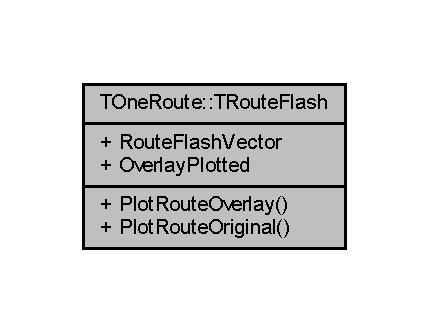
\includegraphics[width=206pt]{class_t_one_route_1_1_t_route_flash__coll__graph}
\end{center}
\end{figure}
\subsection*{Public Member Functions}
\begin{DoxyCompactItemize}
\item 
\mbox{\Hypertarget{class_t_one_route_1_1_t_route_flash_a0292e6d0f38d48da408bb85a60f17944}\label{class_t_one_route_1_1_t_route_flash_a0292e6d0f38d48da408bb85a60f17944}} 
void \mbox{\hyperlink{class_t_one_route_1_1_t_route_flash_a0292e6d0f38d48da408bb85a60f17944}{Plot\+Route\+Overlay}} (int Caller)
\begin{DoxyCompactList}\small\item\em display the overlay (route-\/coloured) graphic \end{DoxyCompactList}\item 
\mbox{\Hypertarget{class_t_one_route_1_1_t_route_flash_a08346a8f10834cc575c175238c7e84ae}\label{class_t_one_route_1_1_t_route_flash_a08346a8f10834cc575c175238c7e84ae}} 
void \mbox{\hyperlink{class_t_one_route_1_1_t_route_flash_a08346a8f10834cc575c175238c7e84ae}{Plot\+Route\+Original}} (int Caller)
\begin{DoxyCompactList}\small\item\em display the original (non route-\/coloured) graphic \end{DoxyCompactList}\end{DoxyCompactItemize}
\subsection*{Public Attributes}
\begin{DoxyCompactItemize}
\item 
\mbox{\Hypertarget{class_t_one_route_1_1_t_route_flash_a5f8fe40f85bdc87247848d2d98685815}\label{class_t_one_route_1_1_t_route_flash_a5f8fe40f85bdc87247848d2d98685815}} 
std\+::vector$<$ \mbox{\hyperlink{class_t_one_route_1_1_t_route_flash_element}{T\+Route\+Flash\+Element}} $>$ {\bfseries Route\+Flash\+Vector}
\item 
\mbox{\Hypertarget{class_t_one_route_1_1_t_route_flash_acc9544214464de94df8becea93062c62}\label{class_t_one_route_1_1_t_route_flash_acc9544214464de94df8becea93062c62}} 
bool \mbox{\hyperlink{class_t_one_route_1_1_t_route_flash_acc9544214464de94df8becea93062c62}{Overlay\+Plotted}}
\begin{DoxyCompactList}\small\item\em flag indicating the graphic that is currently displayed, true for the overlay (route-\/coloured) \end{DoxyCompactList}\end{DoxyCompactItemize}


\subsection{Detailed Description}
The flashing route. 

The documentation for this class was generated from the following files\+:\begin{DoxyCompactItemize}
\item 
Track\+Unit.\+h\item 
Track\+Unit.\+cpp\end{DoxyCompactItemize}

\hypertarget{class_t_one_route_1_1_t_route_flash_element}{}\section{T\+One\+Route\+:\+:T\+Route\+Flash\+Element Class Reference}
\label{class_t_one_route_1_1_t_route_flash_element}\index{T\+One\+Route\+::\+T\+Route\+Flash\+Element@{T\+One\+Route\+::\+T\+Route\+Flash\+Element}}


A single flashing element of a route that flashes during setting.  




{\ttfamily \#include $<$Track\+Unit.\+h$>$}

\subsection*{Public Attributes}
\begin{DoxyCompactItemize}
\item 
\mbox{\Hypertarget{class_t_one_route_1_1_t_route_flash_element_a8cf67aa3834691980c671c4dd1502945}\label{class_t_one_route_1_1_t_route_flash_element_a8cf67aa3834691980c671c4dd1502945}} 
int {\bfseries H\+Loc}
\item 
\mbox{\Hypertarget{class_t_one_route_1_1_t_route_flash_element_a755fdeb7549ed1764d0c8d97e085e940}\label{class_t_one_route_1_1_t_route_flash_element_a755fdeb7549ed1764d0c8d97e085e940}} 
int {\bfseries V\+Loc}
\item 
\mbox{\Hypertarget{class_t_one_route_1_1_t_route_flash_element_ac74a501ef76bca88e523be8b80af9d4c}\label{class_t_one_route_1_1_t_route_flash_element_ac74a501ef76bca88e523be8b80af9d4c}} 
int \mbox{\hyperlink{class_t_one_route_1_1_t_route_flash_element_ac74a501ef76bca88e523be8b80af9d4c}{Track\+Vector\+Position}}
\begin{DoxyCompactList}\small\item\em element values \end{DoxyCompactList}\item 
\mbox{\Hypertarget{class_t_one_route_1_1_t_route_flash_element_ae726a745a5d6760f7cfff05f90392f24}\label{class_t_one_route_1_1_t_route_flash_element_ae726a745a5d6760f7cfff05f90392f24}} 
Graphics\+::\+T\+Bitmap $\ast$ {\bfseries Original\+Graphic}
\item 
Graphics\+::\+T\+Bitmap $\ast$ \mbox{\hyperlink{class_t_one_route_1_1_t_route_flash_element_a9728c9fe83d991d41596efa2cf07129f}{Overlay\+Graphic}}
\end{DoxyCompactItemize}


\subsection{Detailed Description}
A single flashing element of a route that flashes during setting. 

\subsection{Member Data Documentation}
\mbox{\Hypertarget{class_t_one_route_1_1_t_route_flash_element_a9728c9fe83d991d41596efa2cf07129f}\label{class_t_one_route_1_1_t_route_flash_element_a9728c9fe83d991d41596efa2cf07129f}} 
\index{T\+One\+Route\+::\+T\+Route\+Flash\+Element@{T\+One\+Route\+::\+T\+Route\+Flash\+Element}!Overlay\+Graphic@{Overlay\+Graphic}}
\index{Overlay\+Graphic@{Overlay\+Graphic}!T\+One\+Route\+::\+T\+Route\+Flash\+Element@{T\+One\+Route\+::\+T\+Route\+Flash\+Element}}
\subsubsection{\texorpdfstring{Overlay\+Graphic}{OverlayGraphic}}
{\footnotesize\ttfamily Graphics\+::\+T\+Bitmap $\ast$ T\+One\+Route\+::\+T\+Route\+Flash\+Element\+::\+Overlay\+Graphic}

the two graphics, non route-\/coloured and route-\/coloured respectively, these are displayed alternately during flashing 

The documentation for this class was generated from the following file\+:\begin{DoxyCompactItemize}
\item 
Track\+Unit.\+h\end{DoxyCompactItemize}

\hypertarget{struct_t_track_1_1_t_sig_element}{}\section{T\+Track\+:\+:T\+Sig\+Element Struct Reference}
\label{struct_t_track_1_1_t_sig_element}\index{T\+Track\+::\+T\+Sig\+Element@{T\+Track\+::\+T\+Sig\+Element}}


Used as basic elements in a table of signals -\/ see Sig\+Table below.  




{\ttfamily \#include $<$Track\+Unit.\+h$>$}

\subsection*{Public Attributes}
\begin{DoxyCompactItemize}
\item 
\mbox{\Hypertarget{struct_t_track_1_1_t_sig_element_a34471e55de8fcc915046b28706156071}\label{struct_t_track_1_1_t_sig_element_a34471e55de8fcc915046b28706156071}} 
int \mbox{\hyperlink{struct_t_track_1_1_t_sig_element_a34471e55de8fcc915046b28706156071}{Speed\+Tag}}
\begin{DoxyCompactList}\small\item\em the Track\+Element Speed\+Tag value -\/ specifies the signal element \end{DoxyCompactList}\item 
\mbox{\Hypertarget{struct_t_track_1_1_t_sig_element_aaf0195d7519c41c5f2acc57c07b6fb83}\label{struct_t_track_1_1_t_sig_element_aaf0195d7519c41c5f2acc57c07b6fb83}} 
int \mbox{\hyperlink{struct_t_track_1_1_t_sig_element_aaf0195d7519c41c5f2acc57c07b6fb83}{Attribute}}
\begin{DoxyCompactList}\small\item\em the signal state -\/ red, yellow, double yellow or green \end{DoxyCompactList}\item 
\mbox{\Hypertarget{struct_t_track_1_1_t_sig_element_a8e0002e65092d0c2f40adc3980de42c3}\label{struct_t_track_1_1_t_sig_element_a8e0002e65092d0c2f40adc3980de42c3}} 
Graphics\+::\+T\+Bitmap $\ast$ \mbox{\hyperlink{struct_t_track_1_1_t_sig_element_a8e0002e65092d0c2f40adc3980de42c3}{Sig\+Ptr}}
\begin{DoxyCompactList}\small\item\em pointer to the graphic \end{DoxyCompactList}\end{DoxyCompactItemize}


\subsection{Detailed Description}
Used as basic elements in a table of signals -\/ see Sig\+Table below. 

The documentation for this struct was generated from the following file\+:\begin{DoxyCompactItemize}
\item 
Track\+Unit.\+h\end{DoxyCompactItemize}

\hypertarget{class_t_text_handler}{}\section{T\+Text\+Handler Class Reference}
\label{class_t_text_handler}\index{T\+Text\+Handler@{T\+Text\+Handler}}


A single object that handles text management.  




{\ttfamily \#include $<$Text\+Unit.\+h$>$}

\subsection*{Public Types}
\begin{DoxyCompactItemize}
\item 
\mbox{\Hypertarget{class_t_text_handler_a2538805e05af3522211884f3c2426e84}\label{class_t_text_handler_a2538805e05af3522211884f3c2426e84}} 
typedef std\+::vector$<$ \mbox{\hyperlink{class_t_text_item}{T\+Text\+Item}} $>$ {\bfseries T\+Text\+Vector}
\item 
\mbox{\Hypertarget{class_t_text_handler_a691b60d7ecb9bd6f8d8355467f3136e2}\label{class_t_text_handler_a691b60d7ecb9bd6f8d8355467f3136e2}} 
typedef std\+::vector$<$ \mbox{\hyperlink{class_t_text_item}{T\+Text\+Item}} $>$\+::iterator {\bfseries T\+Text\+Vector\+Iterator}
\end{DoxyCompactItemize}
\subsection*{Public Member Functions}
\begin{DoxyCompactItemize}
\item 
\mbox{\Hypertarget{class_t_text_handler_af766ce44ed9a37e5a723a4ef3968ace0}\label{class_t_text_handler_af766ce44ed9a37e5a723a4ef3968ace0}} 
void {\bfseries Set\+New\+H\+Pos} (int Caller, int Text\+Item, int New\+H\+Pos)
\item 
\mbox{\Hypertarget{class_t_text_handler_a65f0033d036358a5cb2ec5f4732e64ee}\label{class_t_text_handler_a65f0033d036358a5cb2ec5f4732e64ee}} 
void {\bfseries Set\+New\+V\+Pos} (int Caller, int Text\+Item, int New\+V\+Pos)
\item 
\mbox{\Hypertarget{class_t_text_handler_a9b78e10ef2f0907a845c0d8ed7ccdede}\label{class_t_text_handler_a9b78e10ef2f0907a845c0d8ed7ccdede}} 
bool {\bfseries Check\+Text\+Elements\+In\+File} (int Caller, std\+::ifstream \&Vec\+File)
\item 
\mbox{\Hypertarget{class_t_text_handler_a0fb5dca23fd07e642c611381b6344746}\label{class_t_text_handler_a0fb5dca23fd07e642c611381b6344746}} 
bool {\bfseries Find\+Text} (int Caller, Ansi\+String Name, int \&H\+Pos, int \&V\+Pos)
\item 
\mbox{\Hypertarget{class_t_text_handler_ad606b1b745b674f0a46cdaa65d09206d}\label{class_t_text_handler_ad606b1b745b674f0a46cdaa65d09206d}} 
bool {\bfseries Text\+Erase} (int Caller, int H\+Position, int V\+Position)
\item 
\mbox{\Hypertarget{class_t_text_handler_a2395c6412e763e1b1141b6dc1d524f8b}\label{class_t_text_handler_a2395c6412e763e1b1141b6dc1d524f8b}} 
bool {\bfseries Text\+Found} (int Caller, int H\+Pos\+Input, int V\+Pos\+Input)
\item 
\mbox{\Hypertarget{class_t_text_handler_a7fa848c67afecfa5fd33d7fee4ab805b}\label{class_t_text_handler_a7fa848c67afecfa5fd33d7fee4ab805b}} 
\mbox{\hyperlink{class_t_text_item}{T\+Text\+Item}} $\ast$ {\bfseries Select\+Text\+Ptr\+At} (int Caller, int At)
\item 
\mbox{\Hypertarget{class_t_text_handler_ac478536f458d9cda8a841953672f6525}\label{class_t_text_handler_ac478536f458d9cda8a841953672f6525}} 
\mbox{\hyperlink{class_t_text_item}{T\+Text\+Item}} $\ast$ {\bfseries Text\+Ptr\+At} (int Caller, int At)
\item 
\mbox{\Hypertarget{class_t_text_handler_a48c65d591fcb76f0a8e86c7f734849b2}\label{class_t_text_handler_a48c65d591fcb76f0a8e86c7f734849b2}} 
unsigned int {\bfseries Select\+Text\+Vector\+Size} (int Caller)
\item 
\mbox{\Hypertarget{class_t_text_handler_a7dfd4e30235878fb01e7387715e0cb0f}\label{class_t_text_handler_a7dfd4e30235878fb01e7387715e0cb0f}} 
unsigned int {\bfseries Text\+Vector\+Size} (int Caller)
\item 
\mbox{\Hypertarget{class_t_text_handler_aee76a9b018b4c80da351f4cb43172681}\label{class_t_text_handler_aee76a9b018b4c80da351f4cb43172681}} 
void {\bfseries Enter\+And\+Display\+New\+Text} (int Caller, \mbox{\hyperlink{class_t_text_item}{T\+Text\+Item}} \&Text, int H\+Pos, int V\+Pos)
\item 
\mbox{\Hypertarget{class_t_text_handler_ae37cbe9dbbc17228e37d8ce2626e176f}\label{class_t_text_handler_ae37cbe9dbbc17228e37d8ce2626e176f}} 
void {\bfseries Load\+Old} (int Caller, std\+::ifstream \&Vec\+File)
\item 
\mbox{\Hypertarget{class_t_text_handler_ab67bb7278c89557bf9cc8bef475afab5}\label{class_t_text_handler_ab67bb7278c89557bf9cc8bef475afab5}} 
void {\bfseries Load\+Text} (int Caller, std\+::ifstream \&Vec\+File)
\item 
\mbox{\Hypertarget{class_t_text_handler_a30f32d9d3267bc8c90298e0ecd3c26fd}\label{class_t_text_handler_a30f32d9d3267bc8c90298e0ecd3c26fd}} 
void {\bfseries Rebuild\+From\+Text\+Vector} (int Caller, \mbox{\hyperlink{class_t_display}{T\+Display}} $\ast$Disp)
\item 
\mbox{\Hypertarget{class_t_text_handler_a07441155bee467c9fb111b8332681466}\label{class_t_text_handler_a07441155bee467c9fb111b8332681466}} 
void {\bfseries Save\+Text} (int Caller, std\+::ofstream \&Vec\+File)
\item 
\mbox{\Hypertarget{class_t_text_handler_ae50027851479dd0f362a75abad793e7a}\label{class_t_text_handler_ae50027851479dd0f362a75abad793e7a}} 
void {\bfseries Text\+Clear} (int Caller)
\item 
\mbox{\Hypertarget{class_t_text_handler_ad8129c58cfa1ecad2fc343efdb96eb5e}\label{class_t_text_handler_ad8129c58cfa1ecad2fc343efdb96eb5e}} 
void {\bfseries Text\+Move} (int Caller, int H\+Pos\+Input, int V\+Pos\+Input, int \&Text\+Item, int \&Text\+Move\+H\+Pos, int \&Text\+Move\+V\+Pos, bool \&Text\+Found\+Flag)
\item 
\mbox{\Hypertarget{class_t_text_handler_a4fd922e73622bb8e2c21d219e977aa0a}\label{class_t_text_handler_a4fd922e73622bb8e2c21d219e977aa0a}} 
void {\bfseries Text\+Vector\+Push} (int Caller, \mbox{\hyperlink{class_t_text_item}{T\+Text\+Item}} \&Text)
\item 
\mbox{\Hypertarget{class_t_text_handler_a599c1a13d78b63a18ebc17550dfa9a0d}\label{class_t_text_handler_a599c1a13d78b63a18ebc17550dfa9a0d}} 
void {\bfseries Text\+Vector\+Reset\+Position} (int Caller, int H\+Offset, int V\+Offset)
\item 
\mbox{\Hypertarget{class_t_text_handler_a7d202827ae62cd288a07431579977539}\label{class_t_text_handler_a7d202827ae62cd288a07431579977539}} 
void {\bfseries Write\+Text\+To\+Image} (int Caller, Graphics\+::\+T\+Bitmap $\ast$Bitmap)
\end{DoxyCompactItemize}
\subsection*{Public Attributes}
\begin{DoxyCompactItemize}
\item 
\mbox{\Hypertarget{class_t_text_handler_a059b11907e0db9c7a847682a455b9cb9}\label{class_t_text_handler_a059b11907e0db9c7a847682a455b9cb9}} 
T\+Text\+Vector {\bfseries Text\+Vector}
\item 
\mbox{\Hypertarget{class_t_text_handler_a5191f5daba7e3f1ea8f0ae82d8067211}\label{class_t_text_handler_a5191f5daba7e3f1ea8f0ae82d8067211}} 
T\+Text\+Vector {\bfseries Select\+Text\+Vector}
\end{DoxyCompactItemize}


\subsection{Detailed Description}
A single object that handles text management. 

The documentation for this class was generated from the following files\+:\begin{DoxyCompactItemize}
\item 
Text\+Unit.\+h\item 
Text\+Unit.\+cpp\end{DoxyCompactItemize}

\hypertarget{class_t_text_item}{}\section{T\+Text\+Item Class Reference}
\label{class_t_text_item}\index{T\+Text\+Item@{T\+Text\+Item}}


A single piece of text that can be displayed on the railway.  




{\ttfamily \#include $<$Text\+Unit.\+h$>$}

\subsection*{Public Member Functions}
\begin{DoxyCompactItemize}
\item 
\mbox{\Hypertarget{class_t_text_item_abb28782b47199def531bc91c70ebe6c8}\label{class_t_text_item_abb28782b47199def531bc91c70ebe6c8}} 
{\bfseries T\+Text\+Item} (int H, int V, Ansi\+String T, T\+Font $\ast$Input\+Font)
\item 
\mbox{\Hypertarget{class_t_text_item_a7715fccdffe55ff5d780c4b6e22d2e7f}\label{class_t_text_item_a7715fccdffe55ff5d780c4b6e22d2e7f}} 
int {\bfseries Get\+Font\+Style\+As\+Int} (int Caller)
\item 
\mbox{\Hypertarget{class_t_text_item_a61c23aca0093a41c1c366c0eac7f80ca}\label{class_t_text_item_a61c23aca0093a41c1c366c0eac7f80ca}} 
void {\bfseries Set\+Font\+Style\+From\+Int} (int Caller, int Input)
\item 
\mbox{\Hypertarget{class_t_text_item_afa20e50741bdae9bed5d81a4038d572a}\label{class_t_text_item_afa20e50741bdae9bed5d81a4038d572a}} 
void {\bfseries Delete\+Text\+Item} (int Caller)
\end{DoxyCompactItemize}
\subsection*{Public Attributes}
\begin{DoxyCompactItemize}
\item 
\mbox{\Hypertarget{class_t_text_item_a4c25a60852b8493f06d26e64241aa98f}\label{class_t_text_item_a4c25a60852b8493f06d26e64241aa98f}} 
Ansi\+String \mbox{\hyperlink{class_t_text_item_a4c25a60852b8493f06d26e64241aa98f}{Text\+String}}
\begin{DoxyCompactList}\small\item\em the text string \end{DoxyCompactList}\item 
\mbox{\Hypertarget{class_t_text_item_a1be1010d3eed8002ab893103a43ffc7b}\label{class_t_text_item_a1be1010d3eed8002ab893103a43ffc7b}} 
int \mbox{\hyperlink{class_t_text_item_a1be1010d3eed8002ab893103a43ffc7b}{H\+Pos}}
\begin{DoxyCompactList}\small\item\em the horizontal position on the railway \end{DoxyCompactList}\item 
\mbox{\Hypertarget{class_t_text_item_a7fc4c3a7d8583931e2ac595006550f9c}\label{class_t_text_item_a7fc4c3a7d8583931e2ac595006550f9c}} 
int \mbox{\hyperlink{class_t_text_item_a7fc4c3a7d8583931e2ac595006550f9c}{V\+Pos}}
\begin{DoxyCompactList}\small\item\em the vertical position on the railway \end{DoxyCompactList}\item 
\mbox{\Hypertarget{class_t_text_item_a0960b6aa95ed04a4e7bc9131dd6e879e}\label{class_t_text_item_a0960b6aa95ed04a4e7bc9131dd6e879e}} 
T\+Font $\ast$ \mbox{\hyperlink{class_t_text_item_a0960b6aa95ed04a4e7bc9131dd6e879e}{Font}}
\begin{DoxyCompactList}\small\item\em the text font \end{DoxyCompactList}\end{DoxyCompactItemize}


\subsection{Detailed Description}
A single piece of text that can be displayed on the railway. 

The documentation for this class was generated from the following files\+:\begin{DoxyCompactItemize}
\item 
Text\+Unit.\+h\item 
Text\+Unit.\+cpp\end{DoxyCompactItemize}

\hypertarget{class_t_track}{}\section{T\+Track Class Reference}
\label{class_t_track}\index{T\+Track@{T\+Track}}


{\ttfamily \#include $<$Track\+Unit.\+h$>$}



Collaboration diagram for T\+Track\+:
\nopagebreak
\begin{figure}[H]
\begin{center}
\leavevmode
\includegraphics[height=550pt]{class_t_track__coll__graph}
\end{center}
\end{figure}
\subsection*{Classes}
\begin{DoxyCompactItemize}
\item 
class \mbox{\hyperlink{class_t_track_1_1_t_active_level_crossing}{T\+Active\+Level\+Crossing}}
\item 
class \mbox{\hyperlink{class_t_track_1_1_t_fixed_track_array}{T\+Fixed\+Track\+Array}}
\begin{DoxyCompactList}\small\item\em Holds an array of Track\+Pieces, only accessible to \mbox{\hyperlink{class_t_track}{T\+Track}}. \end{DoxyCompactList}\item 
struct \mbox{\hyperlink{struct_t_track_1_1_t_sig_element}{T\+Sig\+Element}}
\begin{DoxyCompactList}\small\item\em $<$ used as basic elements in a table of signals -\/ see Sig\+Table below \end{DoxyCompactList}\end{DoxyCompactItemize}
\subsection*{Public Types}
\begin{DoxyCompactItemize}
\item 
\mbox{\Hypertarget{class_t_track_a4c2e42d85ed9151b4983f079f11d6d79}\label{class_t_track_a4c2e42d85ed9151b4983f079f11d6d79}} 
enum {\bfseries T\+Barrier\+State} \{ {\bfseries Raising}, 
{\bfseries Lowering}, 
{\bfseries Up}, 
{\bfseries Down}
 \}
\item 
\mbox{\Hypertarget{class_t_track_a05bacf165698f9502dc7287b01ece848}\label{class_t_track_a05bacf165698f9502dc7287b01ece848}} 
enum \{ {\bfseries Four\+Aspect\+Build}, 
{\bfseries Three\+Aspect\+Build}, 
{\bfseries Two\+Aspect\+Build}, 
{\bfseries Ground\+Signal\+Build}
 \}
\item 
typedef std\+::vector$<$ \mbox{\hyperlink{class_t_track_1_1_t_active_level_crossing}{T\+Active\+Level\+Crossing}} $>$ \mbox{\hyperlink{class_t_track_af124e944cfb44075f390cf5eceaf3e66}{T\+Active\+L\+C\+Vector}}
\item 
typedef std\+::vector$<$ int $>$ \mbox{\hyperlink{class_t_track_a84634d4f5d5ce1928526e8be27e74a72}{T\+L\+C\+Vector}}
\item 
\mbox{\Hypertarget{class_t_track_ac64e15050a0faf07c1b7410d60cbcbe5}\label{class_t_track_ac64e15050a0faf07c1b7410d60cbcbe5}} 
typedef std\+::vector$<$ \mbox{\hyperlink{class_t_track_element}{T\+Track\+Element}} $>$ \mbox{\hyperlink{class_t_track_ac64e15050a0faf07c1b7410d60cbcbe5}{T\+Track\+Vector}}
\begin{DoxyCompactList}\small\item\em vector of Track\+Elements \end{DoxyCompactList}\item 
\mbox{\Hypertarget{class_t_track_a87cc4e8b965e68fd9f02e3a1fc01b6bb}\label{class_t_track_a87cc4e8b965e68fd9f02e3a1fc01b6bb}} 
typedef std\+::vector$<$ \mbox{\hyperlink{class_t_track_element}{T\+Track\+Element}} $>$\+::iterator {\bfseries T\+Track\+Vector\+Iterator}
\item 
\mbox{\Hypertarget{class_t_track_ab03d3109c635a149c57812c89cec63a4}\label{class_t_track_ab03d3109c635a149c57812c89cec63a4}} 
typedef std\+::map$<$ T\+H\+V\+Pair, unsigned int, \mbox{\hyperlink{class_t_map_comp}{T\+Map\+Comp}} $>$ \mbox{\hyperlink{class_t_track_ab03d3109c635a149c57812c89cec63a4}{T\+Track\+Map}}
\begin{DoxyCompactList}\small\item\em map of Track\+Element Track\+Vector\+Positions, H\+Loc \& V\+Loc pair is the key \end{DoxyCompactList}\item 
\mbox{\Hypertarget{class_t_track_a89e099488b224b6b85e2f112c4889fd0}\label{class_t_track_a89e099488b224b6b85e2f112c4889fd0}} 
typedef T\+Track\+Map\+::iterator {\bfseries T\+Track\+Map\+Iterator}
\item 
\mbox{\Hypertarget{class_t_track_a88632999c299ea51ecc1a7eceb60040e}\label{class_t_track_a88632999c299ea51ecc1a7eceb60040e}} 
typedef std\+::pair$<$ T\+H\+V\+Pair, unsigned int $>$ {\bfseries T\+Track\+Map\+Entry}
\item 
\mbox{\Hypertarget{class_t_track_a57d1f751f59c96c16918a044b3d271f7}\label{class_t_track_a57d1f751f59c96c16918a044b3d271f7}} 
typedef std\+::map$<$ T\+H\+V\+Pair, T\+H\+V\+Pair, \mbox{\hyperlink{class_t_map_comp}{T\+Map\+Comp}} $>$ \mbox{\hyperlink{class_t_track_a57d1f751f59c96c16918a044b3d271f7}{T\+Gap\+Map}}
\begin{DoxyCompactList}\small\item\em map of matching gap positions as an H\+Loc/\+V\+Loc pair, with the key being \end{DoxyCompactList}\item 
\mbox{\Hypertarget{class_t_track_a59d0d360b7897d3364135f3882ec495a}\label{class_t_track_a59d0d360b7897d3364135f3882ec495a}} 
typedef T\+Gap\+Map\+::iterator \mbox{\hyperlink{class_t_track_a59d0d360b7897d3364135f3882ec495a}{T\+Gap\+Map\+Iterator}}
\begin{DoxyCompactList}\small\item\em the first gap H\+Loc/\+V\+Loc pair, contains one entry for each pair of matched gaps \end{DoxyCompactList}\item 
\mbox{\Hypertarget{class_t_track_a9f68c117c1cee4a7d767de13a4232925}\label{class_t_track_a9f68c117c1cee4a7d767de13a4232925}} 
typedef std\+::pair$<$ T\+H\+V\+Pair, T\+H\+V\+Pair $>$ {\bfseries T\+Gap\+Map\+Entry}
\item 
\mbox{\Hypertarget{class_t_track_ab54f3c0560218084f75c55ff87409417}\label{class_t_track_ab54f3c0560218084f75c55ff87409417}} 
typedef std\+::multimap$<$ T\+H\+V\+Pair, unsigned int, \mbox{\hyperlink{class_t_map_comp}{T\+Map\+Comp}} $>$ \mbox{\hyperlink{class_t_track_ab54f3c0560218084f75c55ff87409417}{T\+Inactive\+Track2\+Multi\+Map}}
\begin{DoxyCompactList}\small\item\em multimap of inactive Track\+Elements (platforms, \end{DoxyCompactList}\item 
\mbox{\Hypertarget{class_t_track_a6072881896a545945cbcc26e8307bb68}\label{class_t_track_a6072881896a545945cbcc26e8307bb68}} 
typedef T\+Inactive\+Track2\+Multi\+Map\+::iterator \mbox{\hyperlink{class_t_track_a6072881896a545945cbcc26e8307bb68}{T\+Inactive\+Track2\+Multi\+Map\+Iterator}}
\begin{DoxyCompactList}\small\item\em concourses, non-\/station named locations \& parapets) \end{DoxyCompactList}\item 
typedef std\+::pair$<$ \mbox{\hyperlink{class_t_track_a6072881896a545945cbcc26e8307bb68}{T\+Inactive\+Track2\+Multi\+Map\+Iterator}}, \mbox{\hyperlink{class_t_track_a6072881896a545945cbcc26e8307bb68}{T\+Inactive\+Track2\+Multi\+Map\+Iterator}} $>$ \mbox{\hyperlink{class_t_track_a1ac6dda244b2f5a6e27a458f28fc1b1c}{T\+Inactive\+Track\+Range}}
\item 
\mbox{\Hypertarget{class_t_track_ae0a83809dc6f3dabb0f8fd8e9464ac70}\label{class_t_track_ae0a83809dc6f3dabb0f8fd8e9464ac70}} 
typedef std\+::pair$<$ unsigned int, unsigned int $>$ \mbox{\hyperlink{class_t_track_ae0a83809dc6f3dabb0f8fd8e9464ac70}{T\+I\+M\+Pair}}
\begin{DoxyCompactList}\small\item\em Track\+Element pair type used for inactive elements, values are vector positions. \end{DoxyCompactList}\item 
\mbox{\Hypertarget{class_t_track_a4f32231e16e5bdb3485a8f2d51cf27f6}\label{class_t_track_a4f32231e16e5bdb3485a8f2d51cf27f6}} 
typedef std\+::list$<$ int $>$ \mbox{\hyperlink{class_t_track_a4f32231e16e5bdb3485a8f2d51cf27f6}{T\+L\+N\+Pending\+List}}
\begin{DoxyCompactList}\small\item\em type list of location name vector positions (see note below) used during \end{DoxyCompactList}\item 
\mbox{\Hypertarget{class_t_track_a5fe44ea483c447ec227dc2015ffff40c}\label{class_t_track_a5fe44ea483c447ec227dc2015ffff40c}} 
typedef T\+L\+N\+Pending\+List\+::iterator \mbox{\hyperlink{class_t_track_a5fe44ea483c447ec227dc2015ffff40c}{T\+L\+N\+Pending\+List\+Iterator}}
\begin{DoxyCompactList}\small\item\em naming of linked named location elements \end{DoxyCompactList}\item 
\mbox{\Hypertarget{class_t_track_a3005ddcbe9fd2a56040a8a66e6dc0b61}\label{class_t_track_a3005ddcbe9fd2a56040a8a66e6dc0b61}} 
typedef std\+::multimap$<$ T\+H\+V\+Pair, int, \mbox{\hyperlink{class_t_map_comp}{T\+Map\+Comp}} $>$ \mbox{\hyperlink{class_t_track_a3005ddcbe9fd2a56040a8a66e6dc0b61}{T\+L\+N\+Done2\+Multi\+Map}}
\begin{DoxyCompactList}\small\item\em multimap of location name vector positions (see note below) used \end{DoxyCompactList}\item 
\mbox{\Hypertarget{class_t_track_af5a53d40ae46b83d6fa26f03af55d941}\label{class_t_track_af5a53d40ae46b83d6fa26f03af55d941}} 
typedef T\+L\+N\+Done2\+Multi\+Map\+::iterator \mbox{\hyperlink{class_t_track_af5a53d40ae46b83d6fa26f03af55d941}{T\+L\+N\+Done2\+Multi\+Map\+Iterator}}
\begin{DoxyCompactList}\small\item\em during naming of linked named location elements, \textquotesingle{}2\textquotesingle{} because there \end{DoxyCompactList}\item 
\mbox{\Hypertarget{class_t_track_adc8a7f87a6c265601df84db3d38b6219}\label{class_t_track_adc8a7f87a6c265601df84db3d38b6219}} 
typedef std\+::pair$<$ T\+H\+V\+Pair, int $>$ \mbox{\hyperlink{class_t_track_adc8a7f87a6c265601df84db3d38b6219}{T\+L\+N\+Done2\+Multi\+Map\+Entry}}
\begin{DoxyCompactList}\small\item\em can be up to 2 entries (platforms) at a single location \end{DoxyCompactList}\item 
typedef std\+::multimap$<$ Ansi\+String, int $>$ \mbox{\hyperlink{class_t_track_ac68eed5a26013072d6852aa2e6d6f33d}{T\+Location\+Name\+Multi\+Map}}
\item 
\mbox{\Hypertarget{class_t_track_af5ae176b1d8ec7a205557655e8b5c192}\label{class_t_track_af5ae176b1d8ec7a205557655e8b5c192}} 
typedef T\+Location\+Name\+Multi\+Map\+::iterator {\bfseries T\+Location\+Name\+Multi\+Map\+Iterator}
\item 
\mbox{\Hypertarget{class_t_track_acde3e8d68f9bab58afc4543f6bae2696}\label{class_t_track_acde3e8d68f9bab58afc4543f6bae2696}} 
typedef std\+::pair$<$ T\+Location\+Name\+Multi\+Map\+Iterator, T\+Location\+Name\+Multi\+Map\+Iterator $>$ {\bfseries T\+Location\+Name\+Multi\+Map\+Range}
\item 
\mbox{\Hypertarget{class_t_track_ab607b7a616cd970a8f2ac0258db302b2}\label{class_t_track_ab607b7a616cd970a8f2ac0258db302b2}} 
typedef std\+::pair$<$ Ansi\+String, int $>$ {\bfseries T\+Location\+Name\+Multi\+Map\+Entry}
\item 
typedef std\+::map$<$ Ansi\+String, int $>$ \mbox{\hyperlink{class_t_track_af78e1d88c49cebd05b35fc408a5d9d2e}{T\+Active\+Track\+Element\+Name\+Map}}
\item 
\mbox{\Hypertarget{class_t_track_acb3e8471adea42d0882a260e80e33b21}\label{class_t_track_acb3e8471adea42d0882a260e80e33b21}} 
typedef T\+Active\+Track\+Element\+Name\+Map\+::iterator {\bfseries T\+Active\+Track\+Element\+Name\+Iterator}
\item 
\mbox{\Hypertarget{class_t_track_ac63bcf12fb8b775e0ba691b85cc3515b}\label{class_t_track_ac63bcf12fb8b775e0ba691b85cc3515b}} 
typedef std\+::pair$<$ Ansi\+String, int $>$ {\bfseries T\+Active\+Track\+Element\+Name\+Map\+Entry}
\end{DoxyCompactItemize}
\subsection*{Public Member Functions}
\begin{DoxyCompactItemize}
\item 
\mbox{\Hypertarget{class_t_track_a2e0511d60228cefd27d9a52b8dd3cba4}\label{class_t_track_a2e0511d60228cefd27d9a52b8dd3cba4}} 
Ansi\+String \mbox{\hyperlink{class_t_track_a2e0511d60228cefd27d9a52b8dd3cba4}{Get\+Location\+Name}} (unsigned int Inactive\+Track\+Vector\+Position)
\begin{DoxyCompactList}\small\item\em Return location name for a given inactive track vector position. \end{DoxyCompactList}\item 
\mbox{\Hypertarget{class_t_track_a853f6bc248fd0acdf4afe8a5f6c54251}\label{class_t_track_a853f6bc248fd0acdf4afe8a5f6c54251}} 
bool \mbox{\hyperlink{class_t_track_a853f6bc248fd0acdf4afe8a5f6c54251}{Is\+Ready\+For\+Operation}} ()
\begin{DoxyCompactList}\small\item\em Indicates whether or not the railway is ready for saving as a \textquotesingle{}.rly\textquotesingle{} file and for operation. \end{DoxyCompactList}\item 
\mbox{\Hypertarget{class_t_track_aa8386109483977bfaa97909747358149}\label{class_t_track_aa8386109483977bfaa97909747358149}} 
bool \mbox{\hyperlink{class_t_track_aa8386109483977bfaa97909747358149}{Is\+Track\+Finished}} ()
\begin{DoxyCompactList}\small\item\em Indicates whether or not the track has been successfully linked together. \end{DoxyCompactList}\item 
\mbox{\Hypertarget{class_t_track_a400d338422973dd209eb14ba2f621617}\label{class_t_track_a400d338422973dd209eb14ba2f621617}} 
int {\bfseries Get\+Gap\+H\+Loc} ()
\item 
\mbox{\Hypertarget{class_t_track_a365d1f33d669f7a85c0c5b583e37ef43}\label{class_t_track_a365d1f33d669f7a85c0c5b583e37ef43}} 
int {\bfseries Get\+Gap\+V\+Loc} ()
\item 
\mbox{\Hypertarget{class_t_track_a750354d5deccaf7ccdbe8afe8f0f8e35}\label{class_t_track_a750354d5deccaf7ccdbe8afe8f0f8e35}} 
int {\bfseries Get\+H\+Loc\+Max} ()
\item 
\mbox{\Hypertarget{class_t_track_a5d25871e34f26d3c4c878fd4707ed375}\label{class_t_track_a5d25871e34f26d3c4c878fd4707ed375}} 
int {\bfseries Get\+H\+Loc\+Min} ()
\item 
\mbox{\Hypertarget{class_t_track_a5c13595c171f5c7e4aaa6dfc18f4359f}\label{class_t_track_a5c13595c171f5c7e4aaa6dfc18f4359f}} 
int {\bfseries Get\+V\+Loc\+Max} ()
\item 
\mbox{\Hypertarget{class_t_track_ac42bd1e1e148a91396310b1077d2d8e0}\label{class_t_track_ac42bd1e1e148a91396310b1077d2d8e0}} 
int {\bfseries Get\+V\+Loc\+Min} ()
\item 
\mbox{\Hypertarget{class_t_track_aeb515d40cb9b08ed55ce877ffdbc51a5}\label{class_t_track_aeb515d40cb9b08ed55ce877ffdbc51a5}} 
int \mbox{\hyperlink{class_t_track_aeb515d40cb9b08ed55ce877ffdbc51a5}{Get\+Non\+Points\+Opposite\+Link\+Pos}} (int Link\+Pos\+In)
\begin{DoxyCompactList}\small\item\em Return the corresponding link position (track always occupies either links 0 \& 1 or 2 \& 3) \end{DoxyCompactList}\item 
\mbox{\Hypertarget{class_t_track_a55d9415e3ecac804f3345dddd74f9bad}\label{class_t_track_a55d9415e3ecac804f3345dddd74f9bad}} 
int \mbox{\hyperlink{class_t_track_a55d9415e3ecac804f3345dddd74f9bad}{Track\+Vector\+Size}} ()
\begin{DoxyCompactList}\small\item\em Return the number of active track elements. \end{DoxyCompactList}\item 
\mbox{\Hypertarget{class_t_track_a3cae8cc2dc72d74cf0d24dbc4148c591}\label{class_t_track_a3cae8cc2dc72d74cf0d24dbc4148c591}} 
unsigned int \mbox{\hyperlink{class_t_track_a3cae8cc2dc72d74cf0d24dbc4148c591}{Select\+Vector\+Size}} ()
\begin{DoxyCompactList}\small\item\em Return the number of selected active and inactive track elements (via menu items \textquotesingle{}Edit\textquotesingle{} and \textquotesingle{}Select\textquotesingle{}) \end{DoxyCompactList}\item 
\mbox{\Hypertarget{class_t_track_a512c7a382dec9379b6796c73363599e5}\label{class_t_track_a512c7a382dec9379b6796c73363599e5}} 
void \mbox{\hyperlink{class_t_track_a512c7a382dec9379b6796c73363599e5}{Select\+Push}} (\mbox{\hyperlink{class_t_track_element}{T\+Track\+Element}} Track\+Element)
\begin{DoxyCompactList}\small\item\em Store a Track\+Element in the Select\+Vector. \end{DoxyCompactList}\item 
\mbox{\Hypertarget{class_t_track_a212b9df26c2d6653b841912cd4557b8f}\label{class_t_track_a212b9df26c2d6653b841912cd4557b8f}} 
void {\bfseries Select\+Vector\+Clear} ()
\item 
\mbox{\Hypertarget{class_t_track_a453e9074035359dc22be2b15913e4bab}\label{class_t_track_a453e9074035359dc22be2b15913e4bab}} 
void {\bfseries Set\+H\+Loc\+Max} (int H\+Loc)
\item 
\mbox{\Hypertarget{class_t_track_a30e9bd8b4f5e2fb3f01b8c94a98d79f3}\label{class_t_track_a30e9bd8b4f5e2fb3f01b8c94a98d79f3}} 
void {\bfseries Set\+H\+Loc\+Min} (int H\+Loc)
\item 
\mbox{\Hypertarget{class_t_track_a98e6a381eec13868c31a28f450c1a361}\label{class_t_track_a98e6a381eec13868c31a28f450c1a361}} 
void {\bfseries Set\+Track\+Finished} (bool Value)
\item 
\mbox{\Hypertarget{class_t_track_ad33eb8c757120a0fc52ba43c9c8a3293}\label{class_t_track_ad33eb8c757120a0fc52ba43c9c8a3293}} 
void {\bfseries Set\+V\+Loc\+Max} (int V\+Loc)
\item 
\mbox{\Hypertarget{class_t_track_a6459d38cdb82ae38f54f4a1de4935e09}\label{class_t_track_a6459d38cdb82ae38f54f4a1de4935e09}} 
void {\bfseries Set\+V\+Loc\+Min} (int V\+Loc)
\item 
\mbox{\Hypertarget{class_t_track_a0b0e7c333d860841aed4b66b94a6a955}\label{class_t_track_a0b0e7c333d860841aed4b66b94a6a955}} 
bool \mbox{\hyperlink{class_t_track_a0b0e7c333d860841aed4b66b94a6a955}{Active\+Map\+Check}} (int Caller, int H\+Loc, int V\+Loc, int Speed\+Tag)
\begin{DoxyCompactList}\small\item\em Used to check the validity of footbridge links. \end{DoxyCompactList}\item 
\mbox{\Hypertarget{class_t_track_a54678551db16086c8d269808884075d2}\label{class_t_track_a54678551db16086c8d269808884075d2}} 
bool \mbox{\hyperlink{class_t_track_a54678551db16086c8d269808884075d2}{Any\+Linked\+Level\+Crossing\+Elements\+With\+Routes\+Or\+Trains}} (int Caller, int H\+Loc, int V\+Loc, bool \&Train\+Present)
\begin{DoxyCompactList}\small\item\em True if a route or train present on any linked level crossing element. \end{DoxyCompactList}\item 
bool \mbox{\hyperlink{class_t_track_a607c6164af3158c328dd7c3ae25236c7}{Adj\+Element}} (int Caller, int H\+Loc, int V\+Loc, int Speed\+Tag, int \&Found\+Element)
\item 
bool \mbox{\hyperlink{class_t_track_a96a3a6bcd38491f4f00ec2a585c6f170}{Adj\+Named\+Element}} (int Caller, int H\+Loc, int V\+Loc, int Speed\+Tag, Ansi\+String \&Location\+Name, int \&Found\+Element)
\item 
bool \mbox{\hyperlink{class_t_track_a928a29de1b2a916a1c829d40b68963e9}{Blank\+Element\+At}} (int Caller, int At) const
\item 
\mbox{\Hypertarget{class_t_track_a3ff62ece81af00462951a989f3cee4e5}\label{class_t_track_a3ff62ece81af00462951a989f3cee4e5}} 
bool {\bfseries Check\+Active\+L\+C\+Vector} (int Caller, std\+::ifstream \&Vec\+File)
\item 
\mbox{\Hypertarget{class_t_track_a3c3dce0a9200d3c7dc27d26cdd40bb09}\label{class_t_track_a3c3dce0a9200d3c7dc27d26cdd40bb09}} 
bool \mbox{\hyperlink{class_t_track_a3c3dce0a9200d3c7dc27d26cdd40bb09}{Check\+Footbridge\+Links}} (int Caller, \mbox{\hyperlink{class_t_track_element}{T\+Track\+Element}} \&Track\+Element)
\begin{DoxyCompactList}\small\item\em True if a footbridge is linked properly at both ends. \end{DoxyCompactList}\item 
bool \mbox{\hyperlink{class_t_track_a07cde3507d67aff8eac4255ef28fde16}{Check\+Old\+Track\+Elements\+In\+File}} (int Caller, int \&Number\+Of\+Active\+Elements, std\+::ifstream \&Vec\+File)
\item 
\mbox{\Hypertarget{class_t_track_a9ef606dc7da0eb00c5684c80a4891e04}\label{class_t_track_a9ef606dc7da0eb00c5684c80a4891e04}} 
bool \mbox{\hyperlink{class_t_track_a9ef606dc7da0eb00c5684c80a4891e04}{Check\+Track\+Elements\+In\+File}} (int Caller, int \&Number\+Of\+Active\+Elements, std\+::ifstream \&Vec\+File)
\begin{DoxyCompactList}\small\item\em True if Track\+Elements in the file are all valid. \end{DoxyCompactList}\item 
bool \mbox{\hyperlink{class_t_track_a3b4a2e8a16c61a4286fcf34adb000819}{Diagonal\+Fouled\+By\+Train}} (int Caller, int H\+Loc, int V\+Loc, int Diagonal\+Link\+Number, int \&Train\+ID)
\item 
\mbox{\Hypertarget{class_t_track_a35cb615d02e6e4debe2fb2b764adc058}\label{class_t_track_a35cb615d02e6e4debe2fb2b764adc058}} 
bool \mbox{\hyperlink{class_t_track_a35cb615d02e6e4debe2fb2b764adc058}{Element\+In\+L\+N\+Done2\+Multi\+Map}} (int Caller, int Map\+Pos)
\begin{DoxyCompactList}\small\item\em True if the element defined by Map\+Pos is present in L\+N\+Done2\+Multi\+Map, used during location naming. \end{DoxyCompactList}\item 
\mbox{\Hypertarget{class_t_track_a977285544a4e0b017ed5c9670ac38d87}\label{class_t_track_a977285544a4e0b017ed5c9670ac38d87}} 
bool {\bfseries Element\+In\+L\+N\+Pending\+List} (int Caller, int Map\+Pos)
\item 
\mbox{\Hypertarget{class_t_track_a110a199a0c3fd6d2b8fa1cebc0a0a4ed}\label{class_t_track_a110a199a0c3fd6d2b8fa1cebc0a0a4ed}} 
bool \mbox{\hyperlink{class_t_track_a110a199a0c3fd6d2b8fa1cebc0a0a4ed}{Error\+In\+Track\+Before\+Set\+Gaps}} (int Caller, int \&H\+Loc, int \&V\+Loc)
\begin{DoxyCompactList}\small\item\em Check for track errors prior to gap setting -\/ disused as incorporated a time-\/consuming double brute force search. \end{DoxyCompactList}\item 
\mbox{\Hypertarget{class_t_track_a411cfd944b75372ae56937d69fb8b1c5}\label{class_t_track_a411cfd944b75372ae56937d69fb8b1c5}} 
bool \mbox{\hyperlink{class_t_track_a411cfd944b75372ae56937d69fb8b1c5}{Find\+And\+Highlight\+An\+Unset\+Gap}} (int Caller)
\begin{DoxyCompactList}\small\item\em True if there is an unset gap, and if so it is marked with a red circle, used during gap setting. \end{DoxyCompactList}\item 
\mbox{\Hypertarget{class_t_track_aabdf6becaf1d21cc5c654293cc3fc734}\label{class_t_track_aabdf6becaf1d21cc5c654293cc3fc734}} 
bool \mbox{\hyperlink{class_t_track_aabdf6becaf1d21cc5c654293cc3fc734}{Find\+Highest\+Lowest\+And\+Leftmost\+Named\+Elements}} (int Caller, Ansi\+String Name, int \&V\+Pos\+Hi, int \&V\+Pos\+Lo, int \&H\+Pos)
\begin{DoxyCompactList}\small\item\em Used in locating the screen name position for a named location, return true if find an inactive element called \textquotesingle{}Name\textquotesingle{}. \end{DoxyCompactList}\item 
\mbox{\Hypertarget{class_t_track_ad55e3329a208e84e9e7519cc024b7aec}\label{class_t_track_ad55e3329a208e84e9e7519cc024b7aec}} 
bool \mbox{\hyperlink{class_t_track_ad55e3329a208e84e9e7519cc024b7aec}{Find\+Non\+Platform\+Match}} (int Caller, int H\+Loc, int V\+Loc, int \&Position, \mbox{\hyperlink{class_t_track_element}{T\+Track\+Element}} \&Track\+Element)
\begin{DoxyCompactList}\small\item\em True if find a non-\/platform element at H\+Loc \& V\+Loc, and if so return its Track\+Vector position and a reference to it in Track\+Element. \end{DoxyCompactList}\item 
\mbox{\Hypertarget{class_t_track_a4109e356d902de07ebb8848acbee364a}\label{class_t_track_a4109e356d902de07ebb8848acbee364a}} 
bool \mbox{\hyperlink{class_t_track_a4109e356d902de07ebb8848acbee364a}{Find\+Set\+And\+Display\+Matching\+Gap}} (int Caller, int H\+Loc, int V\+Loc)
\begin{DoxyCompactList}\small\item\em True if find an unset gap that matches the gap at H\+Loc \& V\+Loc, if find one mark it with a green circle. \end{DoxyCompactList}\item 
\mbox{\Hypertarget{class_t_track_a794daa0471b473e28ff24c87a92112dc}\label{class_t_track_a794daa0471b473e28ff24c87a92112dc}} 
bool \mbox{\hyperlink{class_t_track_a794daa0471b473e28ff24c87a92112dc}{Gaps\+Unset}} (int Caller)
\begin{DoxyCompactList}\small\item\em True if there are gaps in the railway and any are unset. \end{DoxyCompactList}\item 
\mbox{\Hypertarget{class_t_track_a23030c22d4c98706d1738205242646d9}\label{class_t_track_a23030c22d4c98706d1738205242646d9}} 
bool \mbox{\hyperlink{class_t_track_a23030c22d4c98706d1738205242646d9}{Inactive\+Map\+Check}} (int Caller, int H\+Loc, int V\+Loc, int Speed\+Tag)
\begin{DoxyCompactList}\small\item\em Used to check the validity of footbridge links. \end{DoxyCompactList}\item 
\mbox{\Hypertarget{class_t_track_a5259f2d309f98df4f6e2821e7e71ca81}\label{class_t_track_a5259f2d309f98df4f6e2821e7e71ca81}} 
bool \mbox{\hyperlink{class_t_track_a5259f2d309f98df4f6e2821e7e71ca81}{Is\+A\+Track\+Element\+Adjacent\+To\+Link}} (int Caller, int H\+Loc\+In, int V\+Loc\+In, int Link\+In)
\begin{DoxyCompactList}\small\item\em True if there is an element adjacent to Link\+In for element at H\+Loc \& V\+Loc. \end{DoxyCompactList}\item 
bool \mbox{\hyperlink{class_t_track_a9519d6fa40b71bfcad4d5383634d73dd}{Is\+Element\+Default\+Length}} (int Caller, \mbox{\hyperlink{class_t_track_element}{T\+Track\+Element}} \&Track\+Element, bool First\+Track, bool \&Length\+Different, bool \&Speed\+Different)
\item 
\mbox{\Hypertarget{class_t_track_a7867a4b41fbc25f35eccab0b03cab9ed}\label{class_t_track_a7867a4b41fbc25f35eccab0b03cab9ed}} 
bool \mbox{\hyperlink{class_t_track_a7867a4b41fbc25f35eccab0b03cab9ed}{Is\+Named\+Non\+Station\+Location\+Present}} (int Caller, int H\+Loc, int V\+Loc)
\begin{DoxyCompactList}\small\item\em True if a non-\/station named location at H\+Loc \& V\+Loc. \end{DoxyCompactList}\item 
\mbox{\Hypertarget{class_t_track_a73e781d0ada0b77618b886557f79b115}\label{class_t_track_a73e781d0ada0b77618b886557f79b115}} 
bool \mbox{\hyperlink{class_t_track_a73e781d0ada0b77618b886557f79b115}{Is\+L\+C\+At\+HV}} (int Caller, int H\+Loc, int V\+Loc)
\begin{DoxyCompactList}\small\item\em True if a level crossing is found at H \& V. \end{DoxyCompactList}\item 
\mbox{\Hypertarget{class_t_track_aad258b17c96ace0dbbad3754eb743274}\label{class_t_track_aad258b17c96ace0dbbad3754eb743274}} 
bool \mbox{\hyperlink{class_t_track_aad258b17c96ace0dbbad3754eb743274}{Is\+L\+C\+Barrier\+Down\+At\+HV}} (int Caller, int H\+Loc, int V\+Loc)
\begin{DoxyCompactList}\small\item\em True if an open (to trains) level crossing is found at H \& V. \end{DoxyCompactList}\item 
\mbox{\Hypertarget{class_t_track_a7331fe3693d4a1f2aa76817e66fba995}\label{class_t_track_a7331fe3693d4a1f2aa76817e66fba995}} 
bool \mbox{\hyperlink{class_t_track_a7331fe3693d4a1f2aa76817e66fba995}{Is\+L\+C\+Barrier\+Up\+At\+HV}} (int Caller, int H\+Loc, int V\+Loc)
\begin{DoxyCompactList}\small\item\em True if a closed (to trains) level crossing is found at H \& V. \end{DoxyCompactList}\item 
\mbox{\Hypertarget{class_t_track_a96468affb70f97173d882afefbec9fb2}\label{class_t_track_a96468affb70f97173d882afefbec9fb2}} 
bool \mbox{\hyperlink{class_t_track_a96468affb70f97173d882afefbec9fb2}{Is\+L\+C\+Barrier\+Flashing\+At\+HV}} (int Caller, int H\+Loc, int V\+Loc)
\begin{DoxyCompactList}\small\item\em True if barrier is in process of opening or closing at H \& V. \end{DoxyCompactList}\item 
\mbox{\Hypertarget{class_t_track_adbec6561f4ecd2fa1dabf3e41502b085}\label{class_t_track_adbec6561f4ecd2fa1dabf3e41502b085}} 
bool \mbox{\hyperlink{class_t_track_adbec6561f4ecd2fa1dabf3e41502b085}{Is\+Platform\+Or\+Named\+Non\+Station\+Location\+Present}} (int Caller, int H\+Loc, int V\+Loc)
\begin{DoxyCompactList}\small\item\em True if a non-\/station named location or platform at H\+Loc \& V\+Loc. \end{DoxyCompactList}\item 
\mbox{\Hypertarget{class_t_track_ac0c7fcb151e24dd265a94136db9b6a58}\label{class_t_track_ac0c7fcb151e24dd265a94136db9b6a58}} 
bool \mbox{\hyperlink{class_t_track_ac0c7fcb151e24dd265a94136db9b6a58}{Is\+Track\+Linked}} (int Caller)
\begin{DoxyCompactList}\small\item\em True if track has been successfully linked (not used any more) \end{DoxyCompactList}\item 
bool \mbox{\hyperlink{class_t_track_a17b6095b0c8de0e1493eeebd6d534247}{Link\+Track}} (int Caller, bool \&Loc\+Error, int \&H\+Loc, int \&V\+Loc, bool Final\+Call)
\item 
bool \mbox{\hyperlink{class_t_track_a42f410832651458a4a34769ef95be51b}{Link\+Track\+No\+Messages}} (int Caller, bool Final\+Call)
\item 
\mbox{\Hypertarget{class_t_track_adf9b0df7c51a36a4fca3a4ced7cc4a35}\label{class_t_track_adf9b0df7c51a36a4fca3a4ced7cc4a35}} 
bool \mbox{\hyperlink{class_t_track_adf9b0df7c51a36a4fca3a4ced7cc4a35}{Location\+Name\+Allocated}} (int Caller, Ansi\+String Location\+Name)
\begin{DoxyCompactList}\small\item\em True if a non-\/empty Location\+Name found in Location\+Name\+Multi\+Map. \end{DoxyCompactList}\item 
\mbox{\Hypertarget{class_t_track_ad7d7ef450424ea6aab50db5445c6448c}\label{class_t_track_ad7d7ef450424ea6aab50db5445c6448c}} 
bool \mbox{\hyperlink{class_t_track_ad7d7ef450424ea6aab50db5445c6448c}{Locations\+Not\+Named}} (int Caller)
\begin{DoxyCompactList}\small\item\em True if there are unnamed Named\+Location\+Elements (includes footbridges) \end{DoxyCompactList}\item 
bool \mbox{\hyperlink{class_t_track_aa60a7460b2d95189e8de3817e4ad21f2}{Matching\+Point}} (int Caller, unsigned int Track\+Vector\+Position, unsigned int Diverging\+Position)
\item 
\mbox{\Hypertarget{class_t_track_a198ba6486ccb7cdfb25bdd8c30451d06}\label{class_t_track_a198ba6486ccb7cdfb25bdd8c30451d06}} 
bool \mbox{\hyperlink{class_t_track_a198ba6486ccb7cdfb25bdd8c30451d06}{Named\+Location\+Element\+At}} (int Caller, int H\+Loc, int V\+Loc)
\begin{DoxyCompactList}\small\item\em True if the active or inactive Track\+Element at H\+Loc \& V\+Loc has its Fixed\+Named\+Location\+Element member true. \end{DoxyCompactList}\item 
\mbox{\Hypertarget{class_t_track_ab20c55ecbc1801614695279daa8da0ba}\label{class_t_track_ab20c55ecbc1801614695279daa8da0ba}} 
bool \mbox{\hyperlink{class_t_track_ab20c55ecbc1801614695279daa8da0ba}{No\+Active\+Or\+Inactive\+Track}} (int Caller)
\begin{DoxyCompactList}\small\item\em True if there is no active or inactive track in the railway. \end{DoxyCompactList}\item 
\mbox{\Hypertarget{class_t_track_a2eaa84532799b76a0b42cf6e2611224d}\label{class_t_track_a2eaa84532799b76a0b42cf6e2611224d}} 
bool \mbox{\hyperlink{class_t_track_a2eaa84532799b76a0b42cf6e2611224d}{No\+Active\+Track}} (int Caller)
\begin{DoxyCompactList}\small\item\em True if there is no active track in the railway. \end{DoxyCompactList}\item 
\mbox{\Hypertarget{class_t_track_ab9e1aa42b1d6399d97390f5068bf68b0}\label{class_t_track_ab9e1aa42b1d6399d97390f5068bf68b0}} 
bool \mbox{\hyperlink{class_t_track_ab9e1aa42b1d6399d97390f5068bf68b0}{No\+Gaps}} (int Caller)
\begin{DoxyCompactList}\small\item\em True if there are no gaps. \end{DoxyCompactList}\item 
\mbox{\Hypertarget{class_t_track_ab079bfd6871c5337b29297e7bc2cfe8b}\label{class_t_track_ab079bfd6871c5337b29297e7bc2cfe8b}} 
bool \mbox{\hyperlink{class_t_track_ab079bfd6871c5337b29297e7bc2cfe8b}{No\+Named\+Location\+Elements}} (int Caller)
\begin{DoxyCompactList}\small\item\em True if there are no Named\+Location\+Elements (includes footbridges) \end{DoxyCompactList}\item 
\mbox{\Hypertarget{class_t_track_adb8c5f303e4977a8ea92c7b706a1d4e5}\label{class_t_track_adb8c5f303e4977a8ea92c7b706a1d4e5}} 
bool \mbox{\hyperlink{class_t_track_adb8c5f303e4977a8ea92c7b706a1d4e5}{Non\+Footbridge\+Named\+Location\+Exists}} (int Caller)
\begin{DoxyCompactList}\small\item\em True if there is a platform, Named\+Non\+Station\+Location or Concourse present in the railway. \end{DoxyCompactList}\item 
\mbox{\Hypertarget{class_t_track_a7eba939947b4c035a191ecaaf1b0bb9a}\label{class_t_track_a7eba939947b4c035a191ecaaf1b0bb9a}} 
bool \mbox{\hyperlink{class_t_track_a7eba939947b4c035a191ecaaf1b0bb9a}{One\+Named\+Location\+Element\+At\+Location}} (int Caller, Ansi\+String Location\+Name)
\begin{DoxyCompactList}\small\item\em True if there is at least one named location element with name \textquotesingle{}Location\+Name\textquotesingle{}, used in timetable integrity checking. \end{DoxyCompactList}\item 
bool \mbox{\hyperlink{class_t_track_a9d209cb6e24f67ba12020440a5e42347}{One\+Named\+Location\+Long\+Enough\+For\+Split}} (int Caller, Ansi\+String Location\+Name)
\item 
\mbox{\Hypertarget{class_t_track_aeac90568597c9f13a27fa90c58f9041f}\label{class_t_track_aeac90568597c9f13a27fa90c58f9041f}} 
bool \mbox{\hyperlink{class_t_track_aeac90568597c9f13a27fa90c58f9041f}{Other\+Train\+On\+Track}} (int Caller, int Next\+Pos, int Next\+Entry\+Pos, int Own\+Train\+ID)
\begin{DoxyCompactList}\small\item\em True if another train on Next\+Entry\+Pos track of element at Next\+Pos, whether bridge or not, return false if not, or if Next\+Pos == -\/1, or if only own train on the track. \end{DoxyCompactList}\item 
bool \mbox{\hyperlink{class_t_track_a7c2888cb7acea2b9c65c5f9cc538df66}{Platform\+On\+Signal\+Side}} (int Caller, int H\+Loc, int V\+Loc, int Speed\+Tag, Graphics\+::\+T\+Bitmap $\ast$\&Signal\+Platform\+Graphic)
\item 
bool \mbox{\hyperlink{class_t_track_a5e2e215fae5247206220d301c324e9a0}{Reposition\+And\+Map\+Track}} (int Caller)
\item 
\mbox{\Hypertarget{class_t_track_ac505e8a8f4097b2fc62e16e3a5a2e28b}\label{class_t_track_ac505e8a8f4097b2fc62e16e3a5a2e28b}} 
bool \mbox{\hyperlink{class_t_track_ac505e8a8f4097b2fc62e16e3a5a2e28b}{Reset\+Conn\+Clk\+Check\+Unset\+Gap\+Jumps}} (int Caller)
\begin{DoxyCompactList}\small\item\em Sets all Conns and C\+Lks to -\/1 except for gapjumps that match and are properly set, returns true for any unset gaps. \end{DoxyCompactList}\item 
bool \mbox{\hyperlink{class_t_track_a1be0a43c6b1dc736d981fe7d883d7f01}{Reset\+Gaps\+From\+Gap\+Map}} (int Caller)
\item 
bool \mbox{\hyperlink{class_t_track_a58a2afacadd0f564b474ac0faabc88d4}{Return\+Next\+Inactive\+Track\+Element}} (int Caller, \mbox{\hyperlink{class_t_track_element}{T\+Track\+Element}} \&Next)
\item 
bool \mbox{\hyperlink{class_t_track_a90e1db27659603b72a703c017ee576c8}{Return\+Next\+Track\+Element}} (int Caller, \mbox{\hyperlink{class_t_track_element}{T\+Track\+Element}} \&Next)
\item 
\mbox{\Hypertarget{class_t_track_a4dffe604a7d6b14cce2c94ad7522fb7f}\label{class_t_track_a4dffe604a7d6b14cce2c94ad7522fb7f}} 
bool \mbox{\hyperlink{class_t_track_a4dffe604a7d6b14cce2c94ad7522fb7f}{This\+Named\+Location\+Long\+Enough\+For\+Split}} (int Caller, Ansi\+String Location\+Name, int First\+Named\+Element\+Pos, int \&Second\+Named\+Element\+Pos, int \&First\+Named\+Linked\+Element\+Pos, int \&Second\+Named\+Linked\+Element\+Pos)
\begin{DoxyCompactList}\small\item\em See above under \textquotesingle{}One\+Named\+Location\+Long\+Enough\+For\+Split\textquotesingle{}. \end{DoxyCompactList}\item 
\mbox{\Hypertarget{class_t_track_addd8e149e66c99a295541c9eda13eae4}\label{class_t_track_addd8e149e66c99a295541c9eda13eae4}} 
bool \mbox{\hyperlink{class_t_track_addd8e149e66c99a295541c9eda13eae4}{Timetabled\+Location\+Name\+Allocated}} (int Caller, Ansi\+String Location\+Name)
\begin{DoxyCompactList}\small\item\em True if a non-\/empty Location\+Name found as a timetabled location name i.\+e. not as a continuation name. \end{DoxyCompactList}\item 
\mbox{\Hypertarget{class_t_track_a12d4069a6a201e13a83347c555a465b2}\label{class_t_track_a12d4069a6a201e13a83347c555a465b2}} 
bool \mbox{\hyperlink{class_t_track_a12d4069a6a201e13a83347c555a465b2}{Train\+On\+Link}} (int Caller, int H\+Loc, int V\+Loc, int Link, int \&Train\+ID)
\begin{DoxyCompactList}\small\item\em New at v1.\+2.\+0; checks whether a train present at input location and link and returns its ID if so. \end{DoxyCompactList}\item 
\mbox{\Hypertarget{class_t_track_ac1dc75f1df6278c62f13e23469b80982}\label{class_t_track_ac1dc75f1df6278c62f13e23469b80982}} 
bool \mbox{\hyperlink{class_t_track_ac1dc75f1df6278c62f13e23469b80982}{Try\+To\+Connect\+Track}} (int Caller, bool \&Loc\+Error, int \&H\+Loc, int \&V\+Loc, bool Give\+Messages)
\begin{DoxyCompactList}\small\item\em Handles all tasks associated with track linking, returns true if successful (see also Link\+Track \& Link\+Track\+No\+Messages above) \end{DoxyCompactList}\item 
\mbox{\Hypertarget{class_t_track_a28019284fc6a90e06fc4b27e011484fa}\label{class_t_track_a28019284fc6a90e06fc4b27e011484fa}} 
Graphics\+::\+T\+Bitmap $\ast$ \mbox{\hyperlink{class_t_track_a28019284fc6a90e06fc4b27e011484fa}{Get\+Fillet\+Graphic}} (int Caller, \mbox{\hyperlink{class_t_track_element}{T\+Track\+Element}} Track\+Element)
\begin{DoxyCompactList}\small\item\em Return a pointer to the point fillet (the bit that appears to move when points are changed) for the point and its Attribute specified in Track\+Element. \end{DoxyCompactList}\item 
Graphics\+::\+T\+Bitmap $\ast$ \mbox{\hyperlink{class_t_track_a10027e5b78eb6dfdc246613d78aab53e}{Retrieve\+Striped\+Named\+Location\+Graphics\+Where\+Relevant}} (int Caller, \mbox{\hyperlink{class_t_track_element}{T\+Track\+Element}} Track\+Element)
\item 
int \mbox{\hyperlink{class_t_track_a0510eacbf80200ff27d991606acf9924}{Find\+Closest\+Link\+Position}} (int Caller, int Start\+T\+V\+Position, int End\+T\+V\+Position)
\item 
int \mbox{\hyperlink{class_t_track_a5b63dde2b21a37d5db7e4d078b03a74c}{Get\+Any\+Element\+Opposite\+Link\+Pos}} (int Caller, int Track\+Vector\+Position, int Link\+Pos, bool \&Derail)
\item 
\mbox{\Hypertarget{class_t_track_a54d3b9daeb9ec0b45b0672e7273bf575}\label{class_t_track_a54d3b9daeb9ec0b45b0672e7273bf575}} 
int \mbox{\hyperlink{class_t_track_a54d3b9daeb9ec0b45b0672e7273bf575}{Get\+Track\+Vector\+Position\+From\+String}} (int Caller, Ansi\+String String, bool Give\+Messages)
\begin{DoxyCompactList}\small\item\em Takes the Element\+ID value (an Ansi\+String) (e.\+g. \char`\"{}8-\/13\char`\"{}, \char`\"{}\+N43-\/\+N127\char`\"{}, etc) and returns the corresponding track vector position, if none is found then -\/1 is returned. \end{DoxyCompactList}\item 
\mbox{\Hypertarget{class_t_track_aa0812972d1ae27198c5fbca8aa7b6134}\label{class_t_track_aa0812972d1ae27198c5fbca8aa7b6134}} 
int \mbox{\hyperlink{class_t_track_aa0812972d1ae27198c5fbca8aa7b6134}{Get\+Vector\+Position\+From\+Track\+Map}} (int Caller, int H\+Loc, int V\+Loc, bool \&Found\+Flag)
\begin{DoxyCompactList}\small\item\em Returns the track vector position corresponding to the Hloc \& V\+Loc positions, Found\+Flag indicates whether an element is found or not, and if not -\/1 is returned. \end{DoxyCompactList}\item 
\mbox{\Hypertarget{class_t_track_a72c171ba53777dc2f5fab90877f9bc45}\label{class_t_track_a72c171ba53777dc2f5fab90877f9bc45}} 
int \mbox{\hyperlink{class_t_track_a72c171ba53777dc2f5fab90877f9bc45}{Number\+Of\+Gaps}} (int Caller)
\begin{DoxyCompactList}\small\item\em Returns the number of gaps in the railway. \end{DoxyCompactList}\item 
\mbox{\Hypertarget{class_t_track_a418966e6fefb71b9d0c9b941197832da}\label{class_t_track_a418966e6fefb71b9d0c9b941197832da}} 
\mbox{\hyperlink{class_t_track_ae0a83809dc6f3dabb0f8fd8e9464ac70}{T\+I\+M\+Pair}} \mbox{\hyperlink{class_t_track_a418966e6fefb71b9d0c9b941197832da}{Get\+Vector\+Positions\+From\+Inactive\+Track\+Map}} (int Caller, int H\+Loc, int V\+Loc, bool \&Found\+Flag)
\begin{DoxyCompactList}\small\item\em Similar to Get\+Vector\+Position\+From\+Track\+Map but for inactive elements, a pair is returned because there can be up to 2 platforms at a specific position. \end{DoxyCompactList}\item 
T\+Location\+Name\+Multi\+Map\+Iterator \mbox{\hyperlink{class_t_track_a694370e3ec67d43da1d8333e06d9ebba}{Find\+Named\+Element\+In\+Location\+Name\+Multi\+Map}} (int Caller, Ansi\+String Location\+Name, T\+Track\+Vector\+Iterator Track\+Element, Ansi\+String \&Error\+String)
\item 
\mbox{\Hypertarget{class_t_track_a224071baecc50be0a643711bf9005db2}\label{class_t_track_a224071baecc50be0a643711bf9005db2}} 
\mbox{\hyperlink{class_t_track_element}{T\+Track\+Element}} \& \mbox{\hyperlink{class_t_track_a224071baecc50be0a643711bf9005db2}{Get\+Inactive\+Track\+Element\+From\+Track\+Map}} (int Caller, int H\+Loc, int V\+Loc)
\begin{DoxyCompactList}\small\item\em Return a reference to the inactive element at H\+Loc \& V\+Loc, if no element is found an error is thrown. \end{DoxyCompactList}\item 
\mbox{\Hypertarget{class_t_track_aeb60286bc570dbafab64fe6dc06af2e4}\label{class_t_track_aeb60286bc570dbafab64fe6dc06af2e4}} 
\mbox{\hyperlink{class_t_track_element}{T\+Track\+Element}} \& \mbox{\hyperlink{class_t_track_aeb60286bc570dbafab64fe6dc06af2e4}{Get\+Track\+Element\+From\+Track\+Map}} (int Caller, int H\+Loc, int V\+Loc)
\begin{DoxyCompactList}\small\item\em Return a reference to the element at H\+Loc \& V\+Loc, if no element is found an error is thrown. \end{DoxyCompactList}\item 
\mbox{\Hypertarget{class_t_track_a51f89cf70e94b037f6378cd78003d82b}\label{class_t_track_a51f89cf70e94b037f6378cd78003d82b}} 
\mbox{\hyperlink{class_t_track_element}{T\+Track\+Element}} \& \mbox{\hyperlink{class_t_track_a51f89cf70e94b037f6378cd78003d82b}{Inactive\+Track\+Element\+At}} (int Caller, int At)
\begin{DoxyCompactList}\small\item\em A range-\/checked version of Inactive\+Track\+Element.\+at(\+At) \end{DoxyCompactList}\item 
\mbox{\Hypertarget{class_t_track_a9cddc7b9d02254d44e242ff14758d660}\label{class_t_track_a9cddc7b9d02254d44e242ff14758d660}} 
\mbox{\hyperlink{class_t_track_element}{T\+Track\+Element}} \& \mbox{\hyperlink{class_t_track_a9cddc7b9d02254d44e242ff14758d660}{Select\+Vector\+At}} (int Caller, int At)
\begin{DoxyCompactList}\small\item\em A range-\/checked version of Select\+Vector.\+at(\+At) \end{DoxyCompactList}\item 
\mbox{\Hypertarget{class_t_track_ad377e5a1f152f2e89832c0f9bcfd261f}\label{class_t_track_ad377e5a1f152f2e89832c0f9bcfd261f}} 
\mbox{\hyperlink{class_t_track_element}{T\+Track\+Element}} \& \mbox{\hyperlink{class_t_track_ad377e5a1f152f2e89832c0f9bcfd261f}{Track\+Element\+At}} (int Caller, int At)
\begin{DoxyCompactList}\small\item\em A range-\/checked version of Track\+Element.\+at(\+At) \end{DoxyCompactList}\item 
\mbox{\Hypertarget{class_t_track_ae37fe26f1d8ed9ef0f498ae12347e0ac}\label{class_t_track_ae37fe26f1d8ed9ef0f498ae12347e0ac}} 
T\+Track\+Vector\+Iterator \mbox{\hyperlink{class_t_track_ae37fe26f1d8ed9ef0f498ae12347e0ac}{Get\+Track\+Vector\+Iterator\+From\+Name\+Position}} (int Caller, int Position)
\begin{DoxyCompactList}\small\item\em Takes an adjusted vector position value from either vector (if active, Position = -\/\+True\+Pos -\/1, if inactive, Position = True\+Pos) and returns a pointer to the relevant element. \end{DoxyCompactList}\item 
void \mbox{\hyperlink{class_t_track_a306dfdff414c8edf6f974d21bd9b83ce}{Add\+Name}} (int Caller, T\+Track\+Vector\+Iterator Track\+Element, Ansi\+String Name)
\item 
\mbox{\Hypertarget{class_t_track_a1a3aca3dd4e4bdc7e4c3c254997c2c5a}\label{class_t_track_a1a3aca3dd4e4bdc7e4c3c254997c2c5a}} 
void \mbox{\hyperlink{class_t_track_a1a3aca3dd4e4bdc7e4c3c254997c2c5a}{Build\+Gap\+Map\+From\+Track\+Vector}} (int Caller)
\begin{DoxyCompactList}\small\item\em Examine Track\+Vector and whenever find a new gap pair enter it into Gap\+Map. \end{DoxyCompactList}\item 
void \mbox{\hyperlink{class_t_track_a20a28eaf0308f7aedcfc78ba9eeadea9}{Calc\+H\+Loc\+Min\+Etc}} (int Caller)
\item 
void \mbox{\hyperlink{class_t_track_aa081ea276995a63dfa00fc0ace24f5c5}{Change\+Location\+Name\+Multi\+Map\+Entry}} (int Caller, Ansi\+String New\+Name, T\+Location\+Name\+Multi\+Map\+Iterator S\+N\+Iterator)
\item 
\mbox{\Hypertarget{class_t_track_a6c4ff502fade845fc1b9011cc4532e3a}\label{class_t_track_a6c4ff502fade845fc1b9011cc4532e3a}} 
void \mbox{\hyperlink{class_t_track_a6c4ff502fade845fc1b9011cc4532e3a}{Check\+Gap\+Map}} (int Caller)
\begin{DoxyCompactList}\small\item\em Validity test. \end{DoxyCompactList}\item 
\mbox{\Hypertarget{class_t_track_aaf3f48b8df9877499aaf4c05f804426c}\label{class_t_track_aaf3f48b8df9877499aaf4c05f804426c}} 
void \mbox{\hyperlink{class_t_track_aaf3f48b8df9877499aaf4c05f804426c}{Check\+Location\+Name\+Multi\+Map}} (int Caller)
\begin{DoxyCompactList}\small\item\em Validity test. \end{DoxyCompactList}\item 
\mbox{\Hypertarget{class_t_track_a6fa2d4f2c6c94e2c6b4f7218f5356108}\label{class_t_track_a6fa2d4f2c6c94e2c6b4f7218f5356108}} 
void \mbox{\hyperlink{class_t_track_a6fa2d4f2c6c94e2c6b4f7218f5356108}{Check\+Map\+And\+Inactive\+Track}} (int Caller)
\begin{DoxyCompactList}\small\item\em Validity test. \end{DoxyCompactList}\item 
\mbox{\Hypertarget{class_t_track_a4045fe3f4a71f30a137a7e4581d39231}\label{class_t_track_a4045fe3f4a71f30a137a7e4581d39231}} 
void \mbox{\hyperlink{class_t_track_a4045fe3f4a71f30a137a7e4581d39231}{Check\+Map\+And\+Track}} (int Caller)
\begin{DoxyCompactList}\small\item\em Validity test. \end{DoxyCompactList}\item 
void \mbox{\hyperlink{class_t_track_a2095a52c4b914bf6b29529a2d82043e9}{Decrement\+Values\+In\+Gaps\+And\+Track\+And\+Name\+Maps}} (int Caller, unsigned int Vec\+Pos)
\item 
void \mbox{\hyperlink{class_t_track_af8f925ac5e7301c1094cec76808e1140}{Decrement\+Values\+In\+Inactive\+Track\+And\+Name\+Maps}} (int Caller, unsigned int Vec\+Pos)
\item 
void \mbox{\hyperlink{class_t_track_a433736aed04f76b3d0c39f0696c3bb18}{Enter\+Location\+Name}} (int Caller, Ansi\+String Location\+Name, bool Adding\+Elements)
\item 
void \mbox{\hyperlink{class_t_track_a13a1cc9770c8729d04ad4c0130f91634}{Erase\+Location\+And\+Active\+Track\+Element\+Names}} (int Caller, Ansi\+String Location\+Name)
\item 
void \mbox{\hyperlink{class_t_track_aa7b58c83ca1743ad3e4607ac0af9c71c}{Erase\+Track\+Element}} (int Caller, int H\+Loc\+Input, int V\+Loc\+Input, int \&Erased\+Track\+Vector\+Position, bool \&Track\+Erase\+Successful\+Flag, bool Internal\+Checks)
\item 
void \mbox{\hyperlink{class_t_track_abda5d1209d5a197f1cefb851f567736d}{Get\+Screen\+Positions\+From\+True\+Pos}} (int Caller, int \&Screen\+PosH, int \&Screen\+PosV, int H\+Pos\+True, int V\+Pos\+True)
\item 
void \mbox{\hyperlink{class_t_track_ac57ebd0462a3e0d8323e7b5cbc0e20ca}{Get\+Track\+Locs\+From\+Screen\+Pos}} (int Caller, int \&H\+Loc, int \&V\+Loc, int Screen\+PosH, int Screen\+PosV)
\item 
\mbox{\Hypertarget{class_t_track_a21ad3e4a9e659cf12122691951e19fb6}\label{class_t_track_a21ad3e4a9e659cf12122691951e19fb6}} 
void \mbox{\hyperlink{class_t_track_a21ad3e4a9e659cf12122691951e19fb6}{Get\+True\+Positions\+From\+Screen\+Pos}} (int Caller, int \&H\+Pos, int \&V\+Pos, int Screen\+PosH, int Screen\+PosV)
\begin{DoxyCompactList}\small\item\em Converse of Get\+Screen\+Positions\+From\+True\+Pos. \end{DoxyCompactList}\item 
\mbox{\Hypertarget{class_t_track_a8520abf65484aa83a28329a633836f97}\label{class_t_track_a8520abf65484aa83a28329a633836f97}} 
void \mbox{\hyperlink{class_t_track_a8520abf65484aa83a28329a633836f97}{Length\+Marker}} (int Caller, \mbox{\hyperlink{class_t_display}{T\+Display}} $\ast$Disp)
\begin{DoxyCompactList}\small\item\em Examine all elements in the Track\+Vector and if have a valid length mark the relevant track using Mark\+One\+Length. \end{DoxyCompactList}\item 
\mbox{\Hypertarget{class_t_track_a96563ccfea0293d240212db434f4e3e0}\label{class_t_track_a96563ccfea0293d240212db434f4e3e0}} 
void \mbox{\hyperlink{class_t_track_a96563ccfea0293d240212db434f4e3e0}{Load\+Barriers\+Down\+Vector}} (int Caller, std\+::ifstream \&Vec\+File)
\begin{DoxyCompactList}\small\item\em Load all Barriers\+Down\+Vector values from Session\+File. \end{DoxyCompactList}\item 
void \mbox{\hyperlink{class_t_track_abff18c1d577e257279c816da8868f232}{Load\+Old\+Track}} (int Caller, std\+::ifstream \&Vec\+File)
\item 
\mbox{\Hypertarget{class_t_track_adcd1d019cbdb0d0dbfa44a41dc98ba07}\label{class_t_track_adcd1d019cbdb0d0dbfa44a41dc98ba07}} 
void \mbox{\hyperlink{class_t_track_adcd1d019cbdb0d0dbfa44a41dc98ba07}{Load\+Track}} (int Caller, std\+::ifstream \&Vec\+File)
\begin{DoxyCompactList}\small\item\em Load track elements (active \& inactive) from the file into the relevant vectors and maps, and try to link the resulting track. \end{DoxyCompactList}\item 
\mbox{\Hypertarget{class_t_track_a6cab5ab84e10504ef1c9d39e931d42fe}\label{class_t_track_a6cab5ab84e10504ef1c9d39e931d42fe}} 
void \mbox{\hyperlink{class_t_track_a6cab5ab84e10504ef1c9d39e931d42fe}{Mark\+One\+Length}} (int Caller, \mbox{\hyperlink{class_t_track_element}{T\+Track\+Element}} TE, bool First\+Track, \mbox{\hyperlink{class_t_display}{T\+Display}} $\ast$Disp)
\begin{DoxyCompactList}\small\item\em Mark on screen a track element according to its length and speed limit if either of these differ from their default values. \end{DoxyCompactList}\item 
void \mbox{\hyperlink{class_t_track_a608674798cf48d88d614c8817566126e}{Plot\+And\+Add\+Track\+Element}} (int Caller, int Current\+Tag, int H\+Loc\+Input, int V\+Loc\+Input, bool \&Track\+Plotted\+Flag, bool Internal\+Checks)
\item 
\mbox{\Hypertarget{class_t_track_a9baeb3f155bea71ef42f09c276707562}\label{class_t_track_a9baeb3f155bea71ef42f09c276707562}} 
void \mbox{\hyperlink{class_t_track_a9baeb3f155bea71ef42f09c276707562}{Plot\+L\+C\+Base\+Elements\+Only}} (int Caller, T\+Barrier\+State State, int Base\+Element\+Speed\+Tag, int H\+Loc, int V\+Loc, bool Consec\+Signals, \mbox{\hyperlink{class_t_display}{T\+Display}} $\ast$Disp)
\begin{DoxyCompactList}\small\item\em Just replot the basic track elements at a level crossing (for flashing) \end{DoxyCompactList}\item 
\mbox{\Hypertarget{class_t_track_aa0e977764887fba8aa0dab82ef0b957b}\label{class_t_track_aa0e977764887fba8aa0dab82ef0b957b}} 
void \mbox{\hyperlink{class_t_track_aa0e977764887fba8aa0dab82ef0b957b}{Plot\+Lowered\+Linked\+Level\+Crossing\+Barriers}} (int Caller, int Base\+Element\+Speed\+Tag, int H\+Loc, int V\+Loc, bool Consec\+Signals, \mbox{\hyperlink{class_t_display}{T\+Display}} $\ast$Disp)
\begin{DoxyCompactList}\small\item\em Plot \& open (to trains) all level crossings linked to Track\+Element. \end{DoxyCompactList}\item 
\mbox{\Hypertarget{class_t_track_a85837fb5110486604fab79d42ec60db6}\label{class_t_track_a85837fb5110486604fab79d42ec60db6}} 
void \mbox{\hyperlink{class_t_track_a85837fb5110486604fab79d42ec60db6}{Plot\+Plain\+Lowered\+Linked\+Level\+Crossing\+Barriers\+And\+Set\+Markers}} (int Caller, int Base\+Element\+Speed\+Tag, int H\+Loc, int V\+Loc, \mbox{\hyperlink{class_t_display}{T\+Display}} $\ast$Disp)
\begin{DoxyCompactList}\small\item\em Plot LC elements without any base elements, and set Temp\+Marker true -\/ used in Clearand\+Rebuild\+Railway. \end{DoxyCompactList}\item 
\mbox{\Hypertarget{class_t_track_a1f59015a92ef00604156a44011b4f4c8}\label{class_t_track_a1f59015a92ef00604156a44011b4f4c8}} 
void \mbox{\hyperlink{class_t_track_a1f59015a92ef00604156a44011b4f4c8}{Plot\+Plain\+Raised\+Linked\+Level\+Crossing\+Barriers\+And\+Set\+Markers}} (int Caller, int Base\+Element\+Speed\+Tag, int H\+Loc, int V\+Loc, \mbox{\hyperlink{class_t_display}{T\+Display}} $\ast$Disp)
\begin{DoxyCompactList}\small\item\em Plot LC elements without any base elements, and set Temp\+Marker true -\/ used in Clearand\+Rebuild\+Railway. \end{DoxyCompactList}\item 
\mbox{\Hypertarget{class_t_track_adbaf9ab8b709af9d194603892ac91133}\label{class_t_track_adbaf9ab8b709af9d194603892ac91133}} 
void \mbox{\hyperlink{class_t_track_adbaf9ab8b709af9d194603892ac91133}{Plot\+Raised\+Linked\+Level\+Crossing\+Barriers}} (int Caller, int Base\+Element\+Speed\+Tag, int H\+Loc, int V\+Loc, \mbox{\hyperlink{class_t_display}{T\+Display}} $\ast$Disp)
\begin{DoxyCompactList}\small\item\em Plot \& close (to trains) all level crossings linked to Track\+Element. \end{DoxyCompactList}\item 
\mbox{\Hypertarget{class_t_track_aa638a7e118fb22e648d89adbe814a4a1}\label{class_t_track_aa638a7e118fb22e648d89adbe814a4a1}} 
void \mbox{\hyperlink{class_t_track_aa638a7e118fb22e648d89adbe814a4a1}{Plot\+Gap}} (int Caller, \mbox{\hyperlink{class_t_track_element}{T\+Track\+Element}} Track\+Element, \mbox{\hyperlink{class_t_display}{T\+Display}} $\ast$Disp)
\begin{DoxyCompactList}\small\item\em Plots a gap on screen -\/ may be set or unset. \end{DoxyCompactList}\item 
void \mbox{\hyperlink{class_t_track_af56adb319c7003b8ddac8e55afaee3d2}{Plot\+Points}} (int Caller, \mbox{\hyperlink{class_t_track_element}{T\+Track\+Element}} Track\+Element, \mbox{\hyperlink{class_t_display}{T\+Display}} $\ast$Disp, bool Both\+Fillets)
\item 
\mbox{\Hypertarget{class_t_track_aa5742fbc2eb3f8743dde84005499f89e}\label{class_t_track_aa5742fbc2eb3f8743dde84005499f89e}} 
void \mbox{\hyperlink{class_t_track_aa5742fbc2eb3f8743dde84005499f89e}{Plot\+Signal}} (int Caller, \mbox{\hyperlink{class_t_track_element}{T\+Track\+Element}} Track\+Element, \mbox{\hyperlink{class_t_display}{T\+Display}} $\ast$Disp)
\begin{DoxyCompactList}\small\item\em Plot signals on screen according to their aspect (Attribute value) \end{DoxyCompactList}\item 
\mbox{\Hypertarget{class_t_track_af654985aa4d1c17684f91474fa03ed98}\label{class_t_track_af654985aa4d1c17684f91474fa03ed98}} 
void \mbox{\hyperlink{class_t_track_af654985aa4d1c17684f91474fa03ed98}{Plot\+Small\+Railway}} (int Caller, \mbox{\hyperlink{class_t_display}{T\+Display}} $\ast$Disp)
\begin{DoxyCompactList}\small\item\em Plot on screen the zoomed-\/out railway. \end{DoxyCompactList}\item 
void \mbox{\hyperlink{class_t_track_ab831c2f47850f3a89678491475d52d29}{Plot\+Small\+Red\+Gap}} (int Caller)
\item 
\mbox{\Hypertarget{class_t_track_a9a476cd9b32a351de87591f3db2ddb99}\label{class_t_track_a9a476cd9b32a351de87591f3db2ddb99}} 
void \mbox{\hyperlink{class_t_track_a9a476cd9b32a351de87591f3db2ddb99}{Populate\+L\+C\+Vector}} (int Caller)
\begin{DoxyCompactList}\small\item\em Add all L\+Cs to L\+C\+Vector -\/ note that this contains all LC elements whether linked to others or not. \end{DoxyCompactList}\item 
void \mbox{\hyperlink{class_t_track_a4a948544c9ac877232ec721db8bfc914}{Rebuild\+Location\+Name\+Multi\+Map}} (int Caller)
\item 
void \mbox{\hyperlink{class_t_track_afbd25aa0deb973061c8500a4509136e0}{Rebuild\+Track}} (int Caller, \mbox{\hyperlink{class_t_display}{T\+Display}} $\ast$Disp, bool Both\+Point\+Fillets\+And\+Basic\+L\+Cs)
\item 
void \mbox{\hyperlink{class_t_track_a9430d0a48a27e59f41015c5812aa5de2}{Reset\+All\+Train\+I\+D\+Elements}} (int Caller)
\item 
\mbox{\Hypertarget{class_t_track_ac416bb4b69d75d4c5c0303a2cadd52ca}\label{class_t_track_ac416bb4b69d75d4c5c0303a2cadd52ca}} 
void \mbox{\hyperlink{class_t_track_ac416bb4b69d75d4c5c0303a2cadd52ca}{Reset\+Any\+Non\+Matching\+Gaps}} (int Caller)
\begin{DoxyCompactList}\small\item\em Called by Erase\+Track\+Element after the element has been erased and the vector positions changed, in order to reset a matching gaps if the erased element was a set gap. \end{DoxyCompactList}\item 
\mbox{\Hypertarget{class_t_track_a1a5d8cf5f3a46667a745bfcf4c77ba9d}\label{class_t_track_a1a5d8cf5f3a46667a745bfcf4c77ba9d}} 
void \mbox{\hyperlink{class_t_track_a1a5d8cf5f3a46667a745bfcf4c77ba9d}{Reset\+Level\+Crossings}} (int Caller)
\begin{DoxyCompactList}\small\item\em Set all LC attributes to 0 (closed to trains) \end{DoxyCompactList}\item 
\mbox{\Hypertarget{class_t_track_a84f04a79d9caca625e0b279c5690ddb7}\label{class_t_track_a84f04a79d9caca625e0b279c5690ddb7}} 
void \mbox{\hyperlink{class_t_track_a84f04a79d9caca625e0b279c5690ddb7}{Reset\+Points}} (int Caller)
\begin{DoxyCompactList}\small\item\em Called on exit from operation to reset all points to non-\/diverging or to left fork (Attribute = 0) \end{DoxyCompactList}\item 
\mbox{\Hypertarget{class_t_track_acbb91e9cbc84e3dee44f1ca4de1907e8}\label{class_t_track_acbb91e9cbc84e3dee44f1ca4de1907e8}} 
void \mbox{\hyperlink{class_t_track_acbb91e9cbc84e3dee44f1ca4de1907e8}{Reset\+Signals}} (int Caller)
\begin{DoxyCompactList}\small\item\em Called on exit from operation to reset all signals to red (Attribute = 0) \end{DoxyCompactList}\item 
\mbox{\Hypertarget{class_t_track_a6e1031277500eadfd3a0751e4ca4057b}\label{class_t_track_a6e1031277500eadfd3a0751e4ca4057b}} 
void \mbox{\hyperlink{class_t_track_a6e1031277500eadfd3a0751e4ca4057b}{Save\+Changing\+L\+C\+Vector}} (int Caller, std\+::ofstream \&Out\+File)
\begin{DoxyCompactList}\small\item\em Save all changing vector values (used for error file) \end{DoxyCompactList}\item 
\mbox{\Hypertarget{class_t_track_aabbf9502a68e95e1f9d0b8571d9fb57c}\label{class_t_track_aabbf9502a68e95e1f9d0b8571d9fb57c}} 
void \mbox{\hyperlink{class_t_track_aabbf9502a68e95e1f9d0b8571d9fb57c}{Save\+Session\+Barriers\+Down\+Vector}} (int Caller, std\+::ofstream \&Out\+File)
\begin{DoxyCompactList}\small\item\em Save all vector values to the session file. \end{DoxyCompactList}\item 
\mbox{\Hypertarget{class_t_track_a07acf18405f5192f30f5f412c9182d94}\label{class_t_track_a07acf18405f5192f30f5f412c9182d94}} 
void \mbox{\hyperlink{class_t_track_a07acf18405f5192f30f5f412c9182d94}{Save\+Track}} (int Caller, std\+::ofstream \&Vec\+File)
\begin{DoxyCompactList}\small\item\em Save all active and inactive track elements to Vec\+File. \end{DoxyCompactList}\item 
void \mbox{\hyperlink{class_t_track_a68519138e3b39b6ab9433cc9f7862c64}{Search\+For\+And\+Update\+Location\+Name}} (int Caller, int H\+Loc, int V\+Loc, int Speed\+Tag)
\item 
\mbox{\Hypertarget{class_t_track_ad8d0a63ce71bceab09667aa3623b862d}\label{class_t_track_ad8d0a63ce71bceab09667aa3623b862d}} 
void \mbox{\hyperlink{class_t_track_ad8d0a63ce71bceab09667aa3623b862d}{Set\+All\+Default\+Lengths\+And\+Speed\+Limits}} (int Caller)
\begin{DoxyCompactList}\small\item\em Work through all elements in Track\+Vector setting all lengths \& speed limits to default values -\/ including both tracks for 2-\/track elements. \end{DoxyCompactList}\item 
\mbox{\Hypertarget{class_t_track_a31296f2176bd672769e1852ca90ddd51}\label{class_t_track_a31296f2176bd672769e1852ca90ddd51}} 
void \mbox{\hyperlink{class_t_track_a31296f2176bd672769e1852ca90ddd51}{Set\+Element\+ID}} (int Caller, \mbox{\hyperlink{class_t_track_element}{T\+Track\+Element}} \&Track\+Element)
\begin{DoxyCompactList}\small\item\em Convert the position values for the Track\+Element into an identification string and load in Element\+ID. \end{DoxyCompactList}\item 
\mbox{\Hypertarget{class_t_track_a43c4adf8324c465b90bad0a4dd6761a2}\label{class_t_track_a43c4adf8324c465b90bad0a4dd6761a2}} 
void \mbox{\hyperlink{class_t_track_a43c4adf8324c465b90bad0a4dd6761a2}{Set\+L\+C\+Attribute\+At\+HV}} (int Caller, int H\+Loc, int V\+Loc, int Attr)
\begin{DoxyCompactList}\small\item\em Set LC attribute at H \& V; 0=closed to trains, 1 = open to trains, 2 = changing state = closed to trains. \end{DoxyCompactList}\item 
\mbox{\Hypertarget{class_t_track_a57723388cbfcaf525bf982d8e095949e}\label{class_t_track_a57723388cbfcaf525bf982d8e095949e}} 
void \mbox{\hyperlink{class_t_track_a57723388cbfcaf525bf982d8e095949e}{Set\+Linked\+Level\+Crossing\+Barrier\+Attributes}} (int Caller, int H\+Loc, int V\+Loc, int Attr)
\begin{DoxyCompactList}\small\item\em Set linked LC attributes; 0=closed to trains, 1 = open to trains, 2 = changing state = closed to trains. \end{DoxyCompactList}\item 
void \mbox{\hyperlink{class_t_track_a46b69ee08436c2ff5e41673df04bcf11}{Set\+Station\+Entry\+Stop\+Link\+Posses}} (int Caller)
\item 
\mbox{\Hypertarget{class_t_track_a7fe1e2c641e38da6ab3fdbf20e529d2c}\label{class_t_track_a7fe1e2c641e38da6ab3fdbf20e529d2c}} 
void \mbox{\hyperlink{class_t_track_a7fe1e2c641e38da6ab3fdbf20e529d2c}{Show\+Selected\+Gap}} (int Caller, \mbox{\hyperlink{class_t_display}{T\+Display}} $\ast$Disp)
\begin{DoxyCompactList}\small\item\em Called during gap setting to mark a gap with a red circle -\/ after which the program awaits user selection of the matching gap. \end{DoxyCompactList}\item 
\mbox{\Hypertarget{class_t_track_ae6fe537bbd1e56074a358bf2c6233c71}\label{class_t_track_ae6fe537bbd1e56074a358bf2c6233c71}} 
void \mbox{\hyperlink{class_t_track_ae6fe537bbd1e56074a358bf2c6233c71}{Track\+Clear}} (int Caller)
\begin{DoxyCompactList}\small\item\em Empty the track and inactive track vectors, the corresponding track maps, and Location\+Name\+Multi\+Map. \end{DoxyCompactList}\item 
\mbox{\Hypertarget{class_t_track_a2d8f9445f873689b8e71d3f8efc7c7d3}\label{class_t_track_a2d8f9445f873689b8e71d3f8efc7c7d3}} 
void \mbox{\hyperlink{class_t_track_a2d8f9445f873689b8e71d3f8efc7c7d3}{Track\+Push}} (int Caller, \mbox{\hyperlink{class_t_track_element}{T\+Track\+Element}} Track\+Element)
\begin{DoxyCompactList}\small\item\em Insert Track\+Element into the relevant vector and map, and, if named, insert the name in Location\+Name\+Multi\+Map. \end{DoxyCompactList}\item 
\mbox{\Hypertarget{class_t_track_afb6bf873ba2e4107cf462f9d42dbe33f}\label{class_t_track_afb6bf873ba2e4107cf462f9d42dbe33f}} 
void \mbox{\hyperlink{class_t_track_afb6bf873ba2e4107cf462f9d42dbe33f}{Write\+Operating\+Track\+To\+Image}} (int Caller, Graphics\+::\+T\+Bitmap $\ast$Bitmap)
\begin{DoxyCompactList}\small\item\em Called by T\+Interface\+::\+Save\+Operating\+Image1\+Click to add all track element graphics to the image file in their operating state. \end{DoxyCompactList}\item 
void \mbox{\hyperlink{class_t_track_ab3530b4af2a4b2a9cd1c1b480a19298d}{Write\+Track\+To\+Image}} (int Caller, Graphics\+::\+T\+Bitmap $\ast$Bitmap)
\item 
\mbox{\Hypertarget{class_t_track_a2db41b793217546f23d218294c088996}\label{class_t_track_a2db41b793217546f23d218294c088996}} 
\mbox{\hyperlink{class_t_track_a2db41b793217546f23d218294c088996}{T\+Track}} ()
\begin{DoxyCompactList}\small\item\em Constructor, only one object of this class. \end{DoxyCompactList}\item 
\mbox{\Hypertarget{class_t_track_aefdbe7fe9d1092aa9c543a0bb16c84a0}\label{class_t_track_aefdbe7fe9d1092aa9c543a0bb16c84a0}} 
\mbox{\hyperlink{class_t_track_aefdbe7fe9d1092aa9c543a0bb16c84a0}{$\sim$\+T\+Track}} ()
\begin{DoxyCompactList}\small\item\em Destructor. \end{DoxyCompactList}\end{DoxyCompactItemize}
\subsection*{Public Attributes}
\begin{DoxyCompactItemize}
\item 
\mbox{\Hypertarget{class_t_track_a6fcfdf89bdede9d5772403cd9554e00f}\label{class_t_track_a6fcfdf89bdede9d5772403cd9554e00f}} 
\mbox{\hyperlink{struct_t_track_1_1_t_sig_element}{T\+Sig\+Element}} \mbox{\hyperlink{class_t_track_a6fcfdf89bdede9d5772403cd9554e00f}{Sig\+Table}} \mbox{[}40\mbox{]}
\begin{DoxyCompactList}\small\item\em original table of signals for four aspect \end{DoxyCompactList}\item 
\mbox{\Hypertarget{class_t_track_abe909aa3f0927d7ec0b3d2d711f21fc7}\label{class_t_track_abe909aa3f0927d7ec0b3d2d711f21fc7}} 
\mbox{\hyperlink{struct_t_track_1_1_t_sig_element}{T\+Sig\+Element}} \mbox{\hyperlink{class_t_track_abe909aa3f0927d7ec0b3d2d711f21fc7}{Sig\+Table\+Three\+Aspect}} \mbox{[}40\mbox{]}
\begin{DoxyCompactList}\small\item\em new at version 0.\+6 for three aspect \end{DoxyCompactList}\item 
\mbox{\Hypertarget{class_t_track_a0d95665d2d7c843e82cd502313f7013a}\label{class_t_track_a0d95665d2d7c843e82cd502313f7013a}} 
\mbox{\hyperlink{struct_t_track_1_1_t_sig_element}{T\+Sig\+Element}} \mbox{\hyperlink{class_t_track_a0d95665d2d7c843e82cd502313f7013a}{Sig\+Table\+Two\+Aspect}} \mbox{[}40\mbox{]}
\begin{DoxyCompactList}\small\item\em new at version 0.\+6 for two aspect \end{DoxyCompactList}\item 
\mbox{\Hypertarget{class_t_track_a9973697151cf1bdee2f29dce6ecf82b4}\label{class_t_track_a9973697151cf1bdee2f29dce6ecf82b4}} 
\mbox{\hyperlink{struct_t_track_1_1_t_sig_element}{T\+Sig\+Element}} \mbox{\hyperlink{class_t_track_a9973697151cf1bdee2f29dce6ecf82b4}{Sig\+Table\+Ground\+Signal}} \mbox{[}40\mbox{]}
\begin{DoxyCompactList}\small\item\em new at version 0.\+6 for ground signals \end{DoxyCompactList}\item 
\mbox{\Hypertarget{class_t_track_abda8a4b54dd7c5f2b559eed11a7bac9b}\label{class_t_track_abda8a4b54dd7c5f2b559eed11a7bac9b}} 
Ansi\+String {\bfseries Route\+Fail\+Message}
\item 
\mbox{\Hypertarget{class_t_track_ab31047fd6669faab13b15647b798bf1f}\label{class_t_track_ab31047fd6669faab13b15647b798bf1f}} 
bool \mbox{\hyperlink{class_t_track_ab31047fd6669faab13b15647b798bf1f}{Active\+Track\+Element\+Name\+Map\+Compiled\+Flag}}
\begin{DoxyCompactList}\small\item\em indicates that the Active\+Track\+Element\+Name\+Map has been compiled \end{DoxyCompactList}\item 
\mbox{\Hypertarget{class_t_track_a647fc3b77cb297f9ed22fb2134969518}\label{class_t_track_a647fc3b77cb297f9ed22fb2134969518}} 
bool \mbox{\hyperlink{class_t_track_a647fc3b77cb297f9ed22fb2134969518}{Gap\+Flash\+Flag}}
\begin{DoxyCompactList}\small\item\em true when a pair of connected gaps is flashing \end{DoxyCompactList}\item 
\mbox{\Hypertarget{class_t_track_a95e861b6cc171e005cd3b6e1ce5b011d}\label{class_t_track_a95e861b6cc171e005cd3b6e1ce5b011d}} 
bool \mbox{\hyperlink{class_t_track_a95e861b6cc171e005cd3b6e1ce5b011d}{L\+C\+Change\+Flag}}
\begin{DoxyCompactList}\small\item\em true when L\+Cs changing \end{DoxyCompactList}\item 
\mbox{\Hypertarget{class_t_track_a7d42332d3b0b4122ea7b8f3c6332ee97}\label{class_t_track_a7d42332d3b0b4122ea7b8f3c6332ee97}} 
bool \mbox{\hyperlink{class_t_track_a7d42332d3b0b4122ea7b8f3c6332ee97}{L\+C\+Found\+In\+Auto\+Sigs\+Route}}
\begin{DoxyCompactList}\small\item\em true if found an LC during an automatic route search \end{DoxyCompactList}\item 
\mbox{\Hypertarget{class_t_track_a5d8fb05b298ffb88648aa1993cf4ac2c}\label{class_t_track_a5d8fb05b298ffb88648aa1993cf4ac2c}} 
bool \mbox{\hyperlink{class_t_track_a5d8fb05b298ffb88648aa1993cf4ac2c}{L\+C\+Found\+In\+Auto\+Sigs\+Route\+Message\+Given}}
\begin{DoxyCompactList}\small\item\em true if message given to user, to avoid giving multiple times and to avoid other failure messages being given \end{DoxyCompactList}\item 
\mbox{\Hypertarget{class_t_track_a3be055d3c016ced93635700d7da9a2da}\label{class_t_track_a3be055d3c016ced93635700d7da9a2da}} 
bool \mbox{\hyperlink{class_t_track_a3be055d3c016ced93635700d7da9a2da}{L\+C\+Found\+In\+Route\+Building\+Flag}}
\begin{DoxyCompactList}\small\item\em true if a route set through an LC that is closed to trains (\& therefore needs to be opened) \end{DoxyCompactList}\item 
\mbox{\Hypertarget{class_t_track_a50f518fa93ef56b1570e4102fb691e14}\label{class_t_track_a50f518fa93ef56b1570e4102fb691e14}} 
bool \mbox{\hyperlink{class_t_track_a50f518fa93ef56b1570e4102fb691e14}{Point\+Flash\+Flag}}
\begin{DoxyCompactList}\small\item\em true when points are flashing during manual change \end{DoxyCompactList}\item 
\mbox{\Hypertarget{class_t_track_aa66417417a7767acb35425dfa4754311}\label{class_t_track_aa66417417a7767acb35425dfa4754311}} 
bool \mbox{\hyperlink{class_t_track_aa66417417a7767acb35425dfa4754311}{Route\+Flash\+Flag}}
\begin{DoxyCompactList}\small\item\em true while a route is flashing prior to being set \end{DoxyCompactList}\item 
\mbox{\Hypertarget{class_t_track_a33051ac63ce31022cba42eec28611ca0}\label{class_t_track_a33051ac63ce31022cba42eec28611ca0}} 
float \mbox{\hyperlink{class_t_track_a33051ac63ce31022cba42eec28611ca0}{Level\+Crossing\+Barrier\+Up\+Flash\+Duration}}
\begin{DoxyCompactList}\small\item\em duration of the flash period when level crossing closing to trains \end{DoxyCompactList}\item 
\mbox{\Hypertarget{class_t_track_a6edc256a0cefda4c7a51c79004b83597}\label{class_t_track_a6edc256a0cefda4c7a51c79004b83597}} 
float \mbox{\hyperlink{class_t_track_a6edc256a0cefda4c7a51c79004b83597}{Level\+Crossing\+Barrier\+Down\+Flash\+Duration}}
\begin{DoxyCompactList}\small\item\em duration of the flash period when level crossing opening \end{DoxyCompactList}\item 
\mbox{\Hypertarget{class_t_track_aa64b2f90dd40e8eafb32c048fe045ae2}\label{class_t_track_aa64b2f90dd40e8eafb32c048fe045ae2}} 
int \mbox{\hyperlink{class_t_track_aa64b2f90dd40e8eafb32c048fe045ae2}{Flip\+Array}} \mbox{[}First\+Unused\+Speed\+Tag\+Number\mbox{]}
\begin{DoxyCompactList}\small\item\em holds Track\+Element Speed\+Tag values for \textquotesingle{}flipping\textquotesingle{} via menu items \textquotesingle{}Edit\textquotesingle{} \& \textquotesingle{}Flip\textquotesingle{} \end{DoxyCompactList}\item 
\mbox{\Hypertarget{class_t_track_ab5d97faddc5d764dc7744adbf3c86f39}\label{class_t_track_ab5d97faddc5d764dc7744adbf3c86f39}} 
int {\bfseries Gap\+Flash\+Green\+Position}
\item 
\mbox{\Hypertarget{class_t_track_a351b80cfd4c1a83a4f9c460bf7dce54e}\label{class_t_track_a351b80cfd4c1a83a4f9c460bf7dce54e}} 
int \mbox{\hyperlink{class_t_track_a351b80cfd4c1a83a4f9c460bf7dce54e}{Gap\+Flash\+Red\+Position}}
\begin{DoxyCompactList}\small\item\em Track\+Vector\+Position of the gap element that is flashing green or red. \end{DoxyCompactList}\item 
\mbox{\Hypertarget{class_t_track_a45717d2ba1186b2ff1188b50447ad22a}\label{class_t_track_a45717d2ba1186b2ff1188b50447ad22a}} 
int \mbox{\hyperlink{class_t_track_a45717d2ba1186b2ff1188b50447ad22a}{Mirror\+Array}} \mbox{[}First\+Unused\+Speed\+Tag\+Number\mbox{]}
\begin{DoxyCompactList}\small\item\em holds Track\+Element Speed\+Tag values for \textquotesingle{}mirroring\textquotesingle{} via menu items \textquotesingle{}Edit\textquotesingle{} \& \textquotesingle{}Mirror\textquotesingle{} \end{DoxyCompactList}\item 
\mbox{\Hypertarget{class_t_track_a4cade2b1cabb095c4a52efc729efb44f}\label{class_t_track_a4cade2b1cabb095c4a52efc729efb44f}} 
std\+::map$<$ Ansi\+String, char $>$ \mbox{\hyperlink{class_t_track_a4cade2b1cabb095c4a52efc729efb44f}{Continuation\+Name\+Map}}
\begin{DoxyCompactList}\small\item\em map of all continuation names, char is a dummy \end{DoxyCompactList}\item 
\mbox{\Hypertarget{class_t_track_a5b5b9e68cd57f74466f25f989326d316}\label{class_t_track_a5b5b9e68cd57f74466f25f989326d316}} 
\mbox{\hyperlink{class_t_track_af78e1d88c49cebd05b35fc408a5d9d2e}{T\+Active\+Track\+Element\+Name\+Map}} \mbox{\hyperlink{class_t_track_a5b5b9e68cd57f74466f25f989326d316}{Active\+Track\+Element\+Name\+Map}}
\begin{DoxyCompactList}\small\item\em map of active track element names \end{DoxyCompactList}\item 
\mbox{\Hypertarget{class_t_track_af81ededf353294c66fbdcc4c20ba545f}\label{class_t_track_af81ededf353294c66fbdcc4c20ba545f}} 
\mbox{\hyperlink{class_t_track_af124e944cfb44075f390cf5eceaf3e66}{T\+Active\+L\+C\+Vector}} \mbox{\hyperlink{class_t_track_af81ededf353294c66fbdcc4c20ba545f}{Changing\+L\+C\+Vector}}
\begin{DoxyCompactList}\small\item\em vector of values for changing level crossings -\/ i.\+e. barriers in course of being raised or lowered \end{DoxyCompactList}\item 
\mbox{\Hypertarget{class_t_track_a125f335f138343a30260abc12fa6efd3}\label{class_t_track_a125f335f138343a30260abc12fa6efd3}} 
\mbox{\hyperlink{class_t_track_af124e944cfb44075f390cf5eceaf3e66}{T\+Active\+L\+C\+Vector}} \mbox{\hyperlink{class_t_track_a125f335f138343a30260abc12fa6efd3}{Barriers\+Down\+Vector}}
\begin{DoxyCompactList}\small\item\em vector of L\+Cs with barriers down \end{DoxyCompactList}\item 
\mbox{\Hypertarget{class_t_track_a856fcf6873049774bf2b8b3e28a0c17c}\label{class_t_track_a856fcf6873049774bf2b8b3e28a0c17c}} 
\mbox{\hyperlink{class_t_track_a57d1f751f59c96c16918a044b3d271f7}{T\+Gap\+Map}} \mbox{\hyperlink{class_t_track_a856fcf6873049774bf2b8b3e28a0c17c}{Gap\+Map}}
\begin{DoxyCompactList}\small\item\em map of gaps (see type for more information above) \end{DoxyCompactList}\item 
\mbox{\Hypertarget{class_t_track_a77f6e7d47a768e0867d0975418364959}\label{class_t_track_a77f6e7d47a768e0867d0975418364959}} 
\mbox{\hyperlink{class_t_graphic_element}{T\+Graphic\+Element}} $\ast$ {\bfseries Gap\+Flash\+Green}
\item 
\mbox{\Hypertarget{class_t_track_a5937a66571d1359c961df2b2f4bc53f4}\label{class_t_track_a5937a66571d1359c961df2b2f4bc53f4}} 
\mbox{\hyperlink{class_t_graphic_element}{T\+Graphic\+Element}} $\ast$ \mbox{\hyperlink{class_t_track_a5937a66571d1359c961df2b2f4bc53f4}{Gap\+Flash\+Red}}
\begin{DoxyCompactList}\small\item\em the red \& green circle graphics used to show where the gaps are \end{DoxyCompactList}\item 
\mbox{\Hypertarget{class_t_track_add05819a2f4fc2c2e86d376f78c42493}\label{class_t_track_add05819a2f4fc2c2e86d376f78c42493}} 
\mbox{\hyperlink{class_t_track_ab54f3c0560218084f75c55ff87409417}{T\+Inactive\+Track2\+Multi\+Map}} \mbox{\hyperlink{class_t_track_add05819a2f4fc2c2e86d376f78c42493}{Inactive\+Track2\+Multi\+Map}}
\begin{DoxyCompactList}\small\item\em multimap of inactive Track\+Elements (see type for more information above) \end{DoxyCompactList}\item 
\mbox{\Hypertarget{class_t_track_a15d22ee7fd5080ec731666721cacfca1}\label{class_t_track_a15d22ee7fd5080ec731666721cacfca1}} 
\mbox{\hyperlink{class_t_track_a84634d4f5d5ce1928526e8be27e74a72}{T\+L\+C\+Vector}} \mbox{\hyperlink{class_t_track_a15d22ee7fd5080ec731666721cacfca1}{L\+C\+Vector}}
\begin{DoxyCompactList}\small\item\em vector of level crossing Inactive\+Track\+Vector positions \end{DoxyCompactList}\item 
\mbox{\Hypertarget{class_t_track_a499d1662af74f0fc6bded3f35acae2d6}\label{class_t_track_a499d1662af74f0fc6bded3f35acae2d6}} 
\mbox{\hyperlink{class_t_track_a3005ddcbe9fd2a56040a8a66e6dc0b61}{T\+L\+N\+Done2\+Multi\+Map}} \mbox{\hyperlink{class_t_track_a499d1662af74f0fc6bded3f35acae2d6}{L\+N\+Done2\+Multi\+Map}}
\begin{DoxyCompactList}\small\item\em multimap of processed location name elements (see type for more information above) \end{DoxyCompactList}\item 
\mbox{\Hypertarget{class_t_track_a730140b44a32bb3f92d6012155432efc}\label{class_t_track_a730140b44a32bb3f92d6012155432efc}} 
\mbox{\hyperlink{class_t_track_a4f32231e16e5bdb3485a8f2d51cf27f6}{T\+L\+N\+Pending\+List}} \mbox{\hyperlink{class_t_track_a730140b44a32bb3f92d6012155432efc}{L\+N\+Pending\+List}}
\begin{DoxyCompactList}\small\item\em list of location name elements awaiting processing (see type for more information above) \end{DoxyCompactList}\item 
\mbox{\Hypertarget{class_t_track_ae27a3812ad7f5113bf74f5ff63791a0c}\label{class_t_track_ae27a3812ad7f5113bf74f5ff63791a0c}} 
\mbox{\hyperlink{class_t_track_ac68eed5a26013072d6852aa2e6d6f33d}{T\+Location\+Name\+Multi\+Map}} \mbox{\hyperlink{class_t_track_ae27a3812ad7f5113bf74f5ff63791a0c}{Location\+Name\+Multi\+Map}}
\begin{DoxyCompactList}\small\item\em multimap of location names (see type for more information above) \end{DoxyCompactList}\item 
\mbox{\Hypertarget{class_t_track_a135ff66e8de79bb2eadbd6aadf28b957}\label{class_t_track_a135ff66e8de79bb2eadbd6aadf28b957}} 
\mbox{\hyperlink{class_t_track_ab03d3109c635a149c57812c89cec63a4}{T\+Track\+Map}} \mbox{\hyperlink{class_t_track_a135ff66e8de79bb2eadbd6aadf28b957}{Track\+Map}}
\begin{DoxyCompactList}\small\item\em map of track (see type for more information above) \end{DoxyCompactList}\item 
\mbox{\Hypertarget{class_t_track_a1559c243f46ddcb2c0f8da885eba5942}\label{class_t_track_a1559c243f46ddcb2c0f8da885eba5942}} 
\mbox{\hyperlink{class_t_track_ac64e15050a0faf07c1b7410d60cbcbe5}{T\+Track\+Vector}} {\bfseries Track\+Vector}
\item 
\mbox{\Hypertarget{class_t_track_abe65423511b3512c216857c4b6a189c4}\label{class_t_track_abe65423511b3512c216857c4b6a189c4}} 
\mbox{\hyperlink{class_t_track_ac64e15050a0faf07c1b7410d60cbcbe5}{T\+Track\+Vector}} {\bfseries Inactive\+Track\+Vector}
\item 
\mbox{\Hypertarget{class_t_track_a57abc3eebb9cc311b0f11441666630dd}\label{class_t_track_a57abc3eebb9cc311b0f11441666630dd}} 
\mbox{\hyperlink{class_t_track_ac64e15050a0faf07c1b7410d60cbcbe5}{T\+Track\+Vector}} {\bfseries New\+Vector}
\item 
\mbox{\Hypertarget{class_t_track_a1829522bd2d6b59f94e6b66896eaaa65}\label{class_t_track_a1829522bd2d6b59f94e6b66896eaaa65}} 
\mbox{\hyperlink{class_t_track_ac64e15050a0faf07c1b7410d60cbcbe5}{T\+Track\+Vector}} {\bfseries Distance\+Vector}
\item 
\mbox{\Hypertarget{class_t_track_a5a8edb559dc624c4bcab8ac2d61d83eb}\label{class_t_track_a5a8edb559dc624c4bcab8ac2d61d83eb}} 
\mbox{\hyperlink{class_t_track_ac64e15050a0faf07c1b7410d60cbcbe5}{T\+Track\+Vector}} {\bfseries Distance\+Search\+Vector}
\item 
\mbox{\Hypertarget{class_t_track_aa1317775189eeb24f2f2190789243fce}\label{class_t_track_aa1317775189eeb24f2f2190789243fce}} 
\mbox{\hyperlink{class_t_track_ac64e15050a0faf07c1b7410d60cbcbe5}{T\+Track\+Vector}} \mbox{\hyperlink{class_t_track_aa1317775189eeb24f2f2190789243fce}{Select\+Vector}}
\begin{DoxyCompactList}\small\item\em vectors of Track\+Elements \end{DoxyCompactList}\item 
\mbox{\Hypertarget{class_t_track_a5a3eca45e68b0b2d5604b096e26d79f5}\label{class_t_track_a5a3eca45e68b0b2d5604b096e26d79f5}} 
T\+Track\+Vector\+Iterator \mbox{\hyperlink{class_t_track_a5a3eca45e68b0b2d5604b096e26d79f5}{Next\+Track\+Element\+Ptr}}
\begin{DoxyCompactList}\small\item\em track vector iterator used during cycling through a track vector \end{DoxyCompactList}\item 
\mbox{\Hypertarget{class_t_track_ab012f6fbdca9a4a0354885c557f41736}\label{class_t_track_ab012f6fbdca9a4a0354885c557f41736}} 
enum T\+Track\+:: \{ ... \}  \mbox{\hyperlink{class_t_track_ab012f6fbdca9a4a0354885c557f41736}{Signal\+Aspect\+Build\+Mode}}
\begin{DoxyCompactList}\small\item\em aspect mode for future signal additions \end{DoxyCompactList}\end{DoxyCompactItemize}
\subsection*{Private Attributes}
\begin{DoxyCompactItemize}
\item 
\mbox{\Hypertarget{class_t_track_aa518e921b7809730b4b43e96f7136817}\label{class_t_track_aa518e921b7809730b4b43e96f7136817}} 
\mbox{\hyperlink{class_t_track_1_1_t_fixed_track_array}{T\+Fixed\+Track\+Array}} \mbox{\hyperlink{class_t_track_aa518e921b7809730b4b43e96f7136817}{Fixed\+Track\+Array}}
\begin{DoxyCompactList}\small\item\em the Fixed\+Track\+Piece array object \end{DoxyCompactList}\item 
\mbox{\Hypertarget{class_t_track_a87d65b786df282006e60c97826095892}\label{class_t_track_a87d65b786df282006e60c97826095892}} 
\mbox{\hyperlink{class_t_track_element}{T\+Track\+Element}} {\bfseries Distance\+Start\+Element}
\item 
\mbox{\Hypertarget{class_t_track_a8a68b341049d8b5c05b626fed08cdb33}\label{class_t_track_a8a68b341049d8b5c05b626fed08cdb33}} 
\mbox{\hyperlink{class_t_track_element}{T\+Track\+Element}} \mbox{\hyperlink{class_t_track_a8a68b341049d8b5c05b626fed08cdb33}{Distance\+Continuing\+Element}}
\begin{DoxyCompactList}\small\item\em initially used for track element lengths but since disused \end{DoxyCompactList}\item 
\mbox{\Hypertarget{class_t_track_a3129d1f4b765dea2a15dab78e5e58129}\label{class_t_track_a3129d1f4b765dea2a15dab78e5e58129}} 
bool \mbox{\hyperlink{class_t_track_a3129d1f4b765dea2a15dab78e5e58129}{Track\+Finished}}
\begin{DoxyCompactList}\small\item\em marker for all Conn \& Conn\+Link\+Pos values set \& track complete \end{DoxyCompactList}\item 
\mbox{\Hypertarget{class_t_track_a19b95a52149a0cab545fddace312e0cc}\label{class_t_track_a19b95a52149a0cab545fddace312e0cc}} 
int {\bfseries Gap\+Pos}
\item 
\mbox{\Hypertarget{class_t_track_af57a8d2b11f3618b0502cd757fa41541}\label{class_t_track_af57a8d2b11f3618b0502cd757fa41541}} 
int {\bfseries Gap\+H\+Loc}
\item 
\mbox{\Hypertarget{class_t_track_abb7e520a67eccc292c97444ff395d0c0}\label{class_t_track_abb7e520a67eccc292c97444ff395d0c0}} 
int \mbox{\hyperlink{class_t_track_abb7e520a67eccc292c97444ff395d0c0}{Gap\+V\+Loc}}
\begin{DoxyCompactList}\small\item\em record gap setting info \end{DoxyCompactList}\item 
\mbox{\Hypertarget{class_t_track_aa3a4180a4a3316a5d265964a6ba6b9f8}\label{class_t_track_aa3a4180a4a3316a5d265964a6ba6b9f8}} 
int {\bfseries H\+Loc\+Min}
\item 
\mbox{\Hypertarget{class_t_track_a906deb75070b0e29cf624569c982c23a}\label{class_t_track_a906deb75070b0e29cf624569c982c23a}} 
int {\bfseries V\+Loc\+Min}
\item 
\mbox{\Hypertarget{class_t_track_ab464ea55d7bf8c25d8d5863295209937}\label{class_t_track_ab464ea55d7bf8c25d8d5863295209937}} 
int {\bfseries H\+Loc\+Max}
\item 
\mbox{\Hypertarget{class_t_track_a847326710b5b428b1a8bb54b1d143c26}\label{class_t_track_a847326710b5b428b1a8bb54b1d143c26}} 
int \mbox{\hyperlink{class_t_track_a847326710b5b428b1a8bb54b1d143c26}{V\+Loc\+Max}}
\begin{DoxyCompactList}\small\item\em give extent of railway for use in zoomed in and out displays and in saving railway images \end{DoxyCompactList}\item 
\mbox{\Hypertarget{class_t_track_ae8df4625e0c05c1158f3fc366afe928c}\label{class_t_track_ae8df4625e0c05c1158f3fc366afe928c}} 
int \mbox{\hyperlink{class_t_track_ae8df4625e0c05c1158f3fc366afe928c}{Link\+Check\+Array}} \mbox{[}9\mbox{]}\mbox{[}2\mbox{]}
\begin{DoxyCompactList}\small\item\em array of valid link connecting values, I don\textquotesingle{}t think this is used now \end{DoxyCompactList}\item 
\mbox{\Hypertarget{class_t_track_ab6f605b1cf52a3f8efba5549e19368a8}\label{class_t_track_ab6f605b1cf52a3f8efba5549e19368a8}} 
int \mbox{\hyperlink{class_t_track_ab6f605b1cf52a3f8efba5549e19368a8}{Link\+H\+V\+Array}} \mbox{[}10\mbox{]}\mbox{[}2\mbox{]}
\begin{DoxyCompactList}\small\item\em array used to determine relative horizontal \& vertical track element positions for specific link values \end{DoxyCompactList}\item 
\mbox{\Hypertarget{class_t_track_a8dc657245d548b3b07fdb42e173f3bba}\label{class_t_track_a8dc657245d548b3b07fdb42e173f3bba}} 
int \mbox{\hyperlink{class_t_track_a8dc657245d548b3b07fdb42e173f3bba}{Tag76\+Array}} \mbox{[}23\mbox{]}\mbox{[}3\mbox{]}
\begin{DoxyCompactList}\small\item\em these arrays give valid adjacent named element relative positions for each type of named element, \end{DoxyCompactList}\item 
\mbox{\Hypertarget{class_t_track_a4f05f2ae83cb9f85930df970b7844c4b}\label{class_t_track_a4f05f2ae83cb9f85930df970b7844c4b}} 
int \mbox{\hyperlink{class_t_track_a4f05f2ae83cb9f85930df970b7844c4b}{Tag77\+Array}} \mbox{[}23\mbox{]}\mbox{[}3\mbox{]}
\begin{DoxyCompactList}\small\item\em the numbers -\/ 76, 77 etc -\/ relate to track element element Speed\+Tag values (76 -\/ 79 = platforms, 96 = \end{DoxyCompactList}\item 
\mbox{\Hypertarget{class_t_track_a4b4b28532e1317000b4387a9b37ff981}\label{class_t_track_a4b4b28532e1317000b4387a9b37ff981}} 
int \mbox{\hyperlink{class_t_track_a4b4b28532e1317000b4387a9b37ff981}{Tag78\+Array}} \mbox{[}23\mbox{]}\mbox{[}3\mbox{]}
\begin{DoxyCompactList}\small\item\em concourse, 129 \& 130 = footbridges and 131 = non-\/station named location. \end{DoxyCompactList}\item 
\mbox{\Hypertarget{class_t_track_ab95da137dad09b9c8cd3fc673b80e841}\label{class_t_track_ab95da137dad09b9c8cd3fc673b80e841}} 
int {\bfseries Tag79\+Array} \mbox{[}23\mbox{]}\mbox{[}3\mbox{]}
\item 
\mbox{\Hypertarget{class_t_track_a689870b6bccd25e8b8980e363ad646d0}\label{class_t_track_a689870b6bccd25e8b8980e363ad646d0}} 
int {\bfseries Tag96\+Array} \mbox{[}24\mbox{]}\mbox{[}3\mbox{]}
\item 
\mbox{\Hypertarget{class_t_track_ac54feeb3cf1699bde9e4ac88d76d88fb}\label{class_t_track_ac54feeb3cf1699bde9e4ac88d76d88fb}} 
int {\bfseries Tag129\+Array} \mbox{[}8\mbox{]}\mbox{[}3\mbox{]}
\item 
\mbox{\Hypertarget{class_t_track_a33e00a86d9cb4b0402c08144f9ab563b}\label{class_t_track_a33e00a86d9cb4b0402c08144f9ab563b}} 
int {\bfseries Tag130\+Array} \mbox{[}8\mbox{]}\mbox{[}3\mbox{]}
\item 
\mbox{\Hypertarget{class_t_track_aff5c466da1dda0b20e1f770253ad2813}\label{class_t_track_aff5c466da1dda0b20e1f770253ad2813}} 
int {\bfseries Tag131\+Array} \mbox{[}4\mbox{]}\mbox{[}3\mbox{]}
\item 
\mbox{\Hypertarget{class_t_track_aebfb764fdd1bddb8f82b943e5af9979b}\label{class_t_track_aebfb764fdd1bddb8f82b943e5af9979b}} 
Set$<$ int, 1, 130 $>$ {\bfseries Top\+Plat\+Allowed}
\item 
\mbox{\Hypertarget{class_t_track_a0b2e23790782af830a0b206dcb9d9469}\label{class_t_track_a0b2e23790782af830a0b206dcb9d9469}} 
Set$<$ int, 1, 130 $>$ {\bfseries Bot\+Plat\+Allowed}
\item 
\mbox{\Hypertarget{class_t_track_a70fcf10b4a31240e4d103d04e7116926}\label{class_t_track_a70fcf10b4a31240e4d103d04e7116926}} 
Set$<$ int, 1, 130 $>$ {\bfseries Left\+Plat\+Allowed}
\item 
\mbox{\Hypertarget{class_t_track_a1cde503d01659ec96a735529aca8efcb}\label{class_t_track_a1cde503d01659ec96a735529aca8efcb}} 
Set$<$ int, 1, 130 $>$ {\bfseries Right\+Plat\+Allowed}
\item 
\mbox{\Hypertarget{class_t_track_a44c0c3df5931635e578bfd17d51ecd31}\label{class_t_track_a44c0c3df5931635e578bfd17d51ecd31}} 
Set$<$ int, 1, 130 $>$ {\bfseries Name\+Allowed}
\item 
Set$<$ int, 1, 130 $>$ \mbox{\hyperlink{class_t_track_a29617e6f88e44a7974dc08a371682d0b}{Level\+Crossing\+Allowed}}
\end{DoxyCompactItemize}


\subsection{Detailed Description}
All dynamic track data \& methods. Only one object since only one operating railway

$\ast$\+Note\+: The Track\+Map \& Inactive\+Track\+Map were developed well after the Track\+Vector, to speed up track element searches. It was realised at that time that the maps themselves could contain type \mbox{\hyperlink{class_t_track_element}{T\+Track\+Element}} rather than int (for Track\+Vector\+Position), and that the track vectors could be dispensed with completely. However after an attempt to remove them it was clear that they were far too embedded throughout the program for easy removal, so they were left in. 

\subsection{Member Typedef Documentation}
\mbox{\Hypertarget{class_t_track_af124e944cfb44075f390cf5eceaf3e66}\label{class_t_track_af124e944cfb44075f390cf5eceaf3e66}} 
\index{T\+Track@{T\+Track}!T\+Active\+L\+C\+Vector@{T\+Active\+L\+C\+Vector}}
\index{T\+Active\+L\+C\+Vector@{T\+Active\+L\+C\+Vector}!T\+Track@{T\+Track}}
\subsubsection{\texorpdfstring{T\+Active\+L\+C\+Vector}{TActiveLCVector}}
{\footnotesize\ttfamily typedef std\+::vector$<$\mbox{\hyperlink{class_t_track_1_1_t_active_level_crossing}{T\+Active\+Level\+Crossing}}$>$ \mbox{\hyperlink{class_t_track_af124e944cfb44075f390cf5eceaf3e66}{T\+Track\+::\+T\+Active\+L\+C\+Vector}}}

vector of changing level crossing objects. Note that although a LC may contain several elements there will be only one in the vector when changing, and it might be any of the individual elements. This is because when an entry is made all linked elements have their attributes changed to 2 for changing, so no more are found. This applies both for closing \& opening to trains \mbox{\Hypertarget{class_t_track_af78e1d88c49cebd05b35fc408a5d9d2e}\label{class_t_track_af78e1d88c49cebd05b35fc408a5d9d2e}} 
\index{T\+Track@{T\+Track}!T\+Active\+Track\+Element\+Name\+Map@{T\+Active\+Track\+Element\+Name\+Map}}
\index{T\+Active\+Track\+Element\+Name\+Map@{T\+Active\+Track\+Element\+Name\+Map}!T\+Track@{T\+Track}}
\subsubsection{\texorpdfstring{T\+Active\+Track\+Element\+Name\+Map}{TActiveTrackElementNameMap}}
{\footnotesize\ttfamily typedef std\+::map$<$Ansi\+String, int$>$ \mbox{\hyperlink{class_t_track_af78e1d88c49cebd05b35fc408a5d9d2e}{T\+Track\+::\+T\+Active\+Track\+Element\+Name\+Map}}}

map of Active\+Track\+Element\+Names compiled and used for populating the Location\+Name\+Combo\+Box during timetable creation or editing. Used in place of Location\+Name\+Multi\+Map as that can contain concourses and non-\/station named locations that aren\textquotesingle{}t associated with any track. The second \textquotesingle{}int\textquotesingle{} entry is a dummy, only the list of Ansi\+String names is needed, and being a map it is automatically sorted and without duplicates. \mbox{\Hypertarget{class_t_track_a1ac6dda244b2f5a6e27a458f28fc1b1c}\label{class_t_track_a1ac6dda244b2f5a6e27a458f28fc1b1c}} 
\index{T\+Track@{T\+Track}!T\+Inactive\+Track\+Range@{T\+Inactive\+Track\+Range}}
\index{T\+Inactive\+Track\+Range@{T\+Inactive\+Track\+Range}!T\+Track@{T\+Track}}
\subsubsection{\texorpdfstring{T\+Inactive\+Track\+Range}{TInactiveTrackRange}}
{\footnotesize\ttfamily typedef std\+::pair$<$\mbox{\hyperlink{class_t_track_a6072881896a545945cbcc26e8307bb68}{T\+Inactive\+Track2\+Multi\+Map\+Iterator}}, \mbox{\hyperlink{class_t_track_a6072881896a545945cbcc26e8307bb68}{T\+Inactive\+Track2\+Multi\+Map\+Iterator}}$>$ \mbox{\hyperlink{class_t_track_a1ac6dda244b2f5a6e27a458f28fc1b1c}{T\+Track\+::\+T\+Inactive\+Track\+Range}}}

\textquotesingle{}2\textquotesingle{} because there can be up to 2 entries (platforms) at a single location \mbox{\Hypertarget{class_t_track_a84634d4f5d5ce1928526e8be27e74a72}\label{class_t_track_a84634d4f5d5ce1928526e8be27e74a72}} 
\index{T\+Track@{T\+Track}!T\+L\+C\+Vector@{T\+L\+C\+Vector}}
\index{T\+L\+C\+Vector@{T\+L\+C\+Vector}!T\+Track@{T\+Track}}
\subsubsection{\texorpdfstring{T\+L\+C\+Vector}{TLCVector}}
{\footnotesize\ttfamily typedef std\+::vector$<$int$>$ \mbox{\hyperlink{class_t_track_a84634d4f5d5ce1928526e8be27e74a72}{T\+Track\+::\+T\+L\+C\+Vector}}}

vector of level crossing Inactive\+Track\+Vector positions -\/ note that this contains all LC elements whether linked to others or not \mbox{\Hypertarget{class_t_track_ac68eed5a26013072d6852aa2e6d6f33d}\label{class_t_track_ac68eed5a26013072d6852aa2e6d6f33d}} 
\index{T\+Track@{T\+Track}!T\+Location\+Name\+Multi\+Map@{T\+Location\+Name\+Multi\+Map}}
\index{T\+Location\+Name\+Multi\+Map@{T\+Location\+Name\+Multi\+Map}!T\+Track@{T\+Track}}
\subsubsection{\texorpdfstring{T\+Location\+Name\+Multi\+Map}{TLocationNameMultiMap}}
{\footnotesize\ttfamily typedef std\+::multimap$<$Ansi\+String, int$>$ \mbox{\hyperlink{class_t_track_ac68eed5a26013072d6852aa2e6d6f33d}{T\+Track\+::\+T\+Location\+Name\+Multi\+Map}}}

map of location name vector positions (see note below), one entry for every element that is a Fixed\+Named\+Location\+Element i.\+e platforms, concourses, footbridges \& named non-\/station locations. Hence the only active track elements included are footbridges 

\subsection{Member Function Documentation}
\mbox{\Hypertarget{class_t_track_a306dfdff414c8edf6f974d21bd9b83ce}\label{class_t_track_a306dfdff414c8edf6f974d21bd9b83ce}} 
\index{T\+Track@{T\+Track}!Add\+Name@{Add\+Name}}
\index{Add\+Name@{Add\+Name}!T\+Track@{T\+Track}}
\subsubsection{\texorpdfstring{Add\+Name()}{AddName()}}
{\footnotesize\ttfamily void T\+Track\+::\+Add\+Name (\begin{DoxyParamCaption}\item[{int}]{Caller,  }\item[{T\+Track\+Vector\+Iterator}]{Track\+Element,  }\item[{Ansi\+String}]{Name }\end{DoxyParamCaption})}

Track\+Element.\+Location\+Name becomes \textquotesingle{}Name\textquotesingle{} (for active and inactive elements) and, if Track\+Element is a platform or named non-\/station location, any active element at the same H\+Loc \& V\+Loc position has its Active\+Track\+Element\+Name set to \textquotesingle{}Name\textquotesingle{}. \mbox{\Hypertarget{class_t_track_a607c6164af3158c328dd7c3ae25236c7}\label{class_t_track_a607c6164af3158c328dd7c3ae25236c7}} 
\index{T\+Track@{T\+Track}!Adj\+Element@{Adj\+Element}}
\index{Adj\+Element@{Adj\+Element}!T\+Track@{T\+Track}}
\subsubsection{\texorpdfstring{Adj\+Element()}{AdjElement()}}
{\footnotesize\ttfamily bool T\+Track\+::\+Adj\+Element (\begin{DoxyParamCaption}\item[{int}]{Caller,  }\item[{int}]{H\+Loc,  }\item[{int}]{V\+Loc,  }\item[{int}]{Speed\+Tag,  }\item[{int \&}]{Found\+Element }\end{DoxyParamCaption})}

Used during location naming to check for adjacent named elements to a given element at H\+Loc \& V\+Loc with a specific Speed\+Tag, and if found allow that element to be inserted into the L\+N\+Pending\+List for naming similarly \mbox{\Hypertarget{class_t_track_a96a3a6bcd38491f4f00ec2a585c6f170}\label{class_t_track_a96a3a6bcd38491f4f00ec2a585c6f170}} 
\index{T\+Track@{T\+Track}!Adj\+Named\+Element@{Adj\+Named\+Element}}
\index{Adj\+Named\+Element@{Adj\+Named\+Element}!T\+Track@{T\+Track}}
\subsubsection{\texorpdfstring{Adj\+Named\+Element()}{AdjNamedElement()}}
{\footnotesize\ttfamily bool T\+Track\+::\+Adj\+Named\+Element (\begin{DoxyParamCaption}\item[{int}]{Caller,  }\item[{int}]{H\+Loc,  }\item[{int}]{V\+Loc,  }\item[{int}]{Speed\+Tag,  }\item[{Ansi\+String \&}]{Location\+Name,  }\item[{int \&}]{Found\+Element }\end{DoxyParamCaption})}

Used in Search\+For\+And\+Update\+Location\+Name to check for adjacent named elements to a given element at H\+Loc \& V\+Loc with a specific Speed\+Tag, and if found allow that name to be used for this element and all other named elements that are linked to it \mbox{\Hypertarget{class_t_track_a928a29de1b2a916a1c829d40b68963e9}\label{class_t_track_a928a29de1b2a916a1c829d40b68963e9}} 
\index{T\+Track@{T\+Track}!Blank\+Element\+At@{Blank\+Element\+At}}
\index{Blank\+Element\+At@{Blank\+Element\+At}!T\+Track@{T\+Track}}
\subsubsection{\texorpdfstring{Blank\+Element\+At()}{BlankElementAt()}}
{\footnotesize\ttfamily bool T\+Track\+::\+Blank\+Element\+At (\begin{DoxyParamCaption}\item[{int}]{Caller,  }\item[{int}]{At }\end{DoxyParamCaption}) const}

True for a blank (Speed\+Tag == 0) element at a specific Trackvector position, no longer used after Track\+Erase changed (now Erase\+Track\+Element) so that blank elements aren\textquotesingle{}t used \mbox{\Hypertarget{class_t_track_a20a28eaf0308f7aedcfc78ba9eeadea9}\label{class_t_track_a20a28eaf0308f7aedcfc78ba9eeadea9}} 
\index{T\+Track@{T\+Track}!Calc\+H\+Loc\+Min\+Etc@{Calc\+H\+Loc\+Min\+Etc}}
\index{Calc\+H\+Loc\+Min\+Etc@{Calc\+H\+Loc\+Min\+Etc}!T\+Track@{T\+Track}}
\subsubsection{\texorpdfstring{Calc\+H\+Loc\+Min\+Etc()}{CalcHLocMinEtc()}}
{\footnotesize\ttfamily void T\+Track\+::\+Calc\+H\+Loc\+Min\+Etc (\begin{DoxyParamCaption}\item[{int}]{Caller }\end{DoxyParamCaption})}

Examine Track\+Vector, Inactive\+Track\+Vector and Text\+Vector, and set the values that indicate the extent of the railway (H\+Loc\+Min, V\+Loc\+Min, H\+Loc\+Max \& V\+Loc\+Max) for use in zoomed in and out displays and in saving railway images \mbox{\Hypertarget{class_t_track_aa081ea276995a63dfa00fc0ace24f5c5}\label{class_t_track_aa081ea276995a63dfa00fc0ace24f5c5}} 
\index{T\+Track@{T\+Track}!Change\+Location\+Name\+Multi\+Map\+Entry@{Change\+Location\+Name\+Multi\+Map\+Entry}}
\index{Change\+Location\+Name\+Multi\+Map\+Entry@{Change\+Location\+Name\+Multi\+Map\+Entry}!T\+Track@{T\+Track}}
\subsubsection{\texorpdfstring{Change\+Location\+Name\+Multi\+Map\+Entry()}{ChangeLocationNameMultiMapEntry()}}
{\footnotesize\ttfamily void T\+Track\+::\+Change\+Location\+Name\+Multi\+Map\+Entry (\begin{DoxyParamCaption}\item[{int}]{Caller,  }\item[{Ansi\+String}]{New\+Name,  }\item[{T\+Location\+Name\+Multi\+Map\+Iterator}]{S\+N\+Iterator }\end{DoxyParamCaption})}

Changes the Location\+Name in the name multimap to New\+Name at the location pointed to by the T\+Location\+Name\+Multi\+Map\+Iterator from whatever it was before. Accepts null entries so that a formerly named element can have the name changed to \char`\"{}\char`\"{}. \mbox{\Hypertarget{class_t_track_a07cde3507d67aff8eac4255ef28fde16}\label{class_t_track_a07cde3507d67aff8eac4255ef28fde16}} 
\index{T\+Track@{T\+Track}!Check\+Old\+Track\+Elements\+In\+File@{Check\+Old\+Track\+Elements\+In\+File}}
\index{Check\+Old\+Track\+Elements\+In\+File@{Check\+Old\+Track\+Elements\+In\+File}!T\+Track@{T\+Track}}
\subsubsection{\texorpdfstring{Check\+Old\+Track\+Elements\+In\+File()}{CheckOldTrackElementsInFile()}}
{\footnotesize\ttfamily bool T\+Track\+::\+Check\+Old\+Track\+Elements\+In\+File (\begin{DoxyParamCaption}\item[{int}]{Caller,  }\item[{int \&}]{Number\+Of\+Active\+Elements,  }\item[{std\+::ifstream \&}]{Vec\+File }\end{DoxyParamCaption})}

Version of Check\+Track\+Elements\+In\+File prior to its being updated

Used when changes made to Check\+Track\+Elements\+In\+File in order to allow existing saved railways to be loaded prior to resaving in the new format compatible with the new Check\+Track\+Elements\+In\+File \mbox{\Hypertarget{class_t_track_a2095a52c4b914bf6b29529a2d82043e9}\label{class_t_track_a2095a52c4b914bf6b29529a2d82043e9}} 
\index{T\+Track@{T\+Track}!Decrement\+Values\+In\+Gaps\+And\+Track\+And\+Name\+Maps@{Decrement\+Values\+In\+Gaps\+And\+Track\+And\+Name\+Maps}}
\index{Decrement\+Values\+In\+Gaps\+And\+Track\+And\+Name\+Maps@{Decrement\+Values\+In\+Gaps\+And\+Track\+And\+Name\+Maps}!T\+Track@{T\+Track}}
\subsubsection{\texorpdfstring{Decrement\+Values\+In\+Gaps\+And\+Track\+And\+Name\+Maps()}{DecrementValuesInGapsAndTrackAndNameMaps()}}
{\footnotesize\ttfamily void T\+Track\+::\+Decrement\+Values\+In\+Gaps\+And\+Track\+And\+Name\+Maps (\begin{DoxyParamCaption}\item[{int}]{Caller,  }\item[{unsigned int}]{Vec\+Pos }\end{DoxyParamCaption})}

After an element has been erased from the Track\+Vector, all the later elements are moved down one. This function decrements the position values for all values above that of the erased element in the gap elements, Track\+Map and Location\+Name\+Multi\+Map. \mbox{\Hypertarget{class_t_track_af8f925ac5e7301c1094cec76808e1140}\label{class_t_track_af8f925ac5e7301c1094cec76808e1140}} 
\index{T\+Track@{T\+Track}!Decrement\+Values\+In\+Inactive\+Track\+And\+Name\+Maps@{Decrement\+Values\+In\+Inactive\+Track\+And\+Name\+Maps}}
\index{Decrement\+Values\+In\+Inactive\+Track\+And\+Name\+Maps@{Decrement\+Values\+In\+Inactive\+Track\+And\+Name\+Maps}!T\+Track@{T\+Track}}
\subsubsection{\texorpdfstring{Decrement\+Values\+In\+Inactive\+Track\+And\+Name\+Maps()}{DecrementValuesInInactiveTrackAndNameMaps()}}
{\footnotesize\ttfamily void T\+Track\+::\+Decrement\+Values\+In\+Inactive\+Track\+And\+Name\+Maps (\begin{DoxyParamCaption}\item[{int}]{Caller,  }\item[{unsigned int}]{Vec\+Pos }\end{DoxyParamCaption})}

After an element has been erased from the Inactive\+Track\+Vector, all the later elements are moved down one. This function decrements the position values for all values above that of the erased element in both Inactive\+Track2\+Multi\+Map and Location\+Name\+Multi\+Map. \mbox{\Hypertarget{class_t_track_a3b4a2e8a16c61a4286fcf34adb000819}\label{class_t_track_a3b4a2e8a16c61a4286fcf34adb000819}} 
\index{T\+Track@{T\+Track}!Diagonal\+Fouled\+By\+Train@{Diagonal\+Fouled\+By\+Train}}
\index{Diagonal\+Fouled\+By\+Train@{Diagonal\+Fouled\+By\+Train}!T\+Track@{T\+Track}}
\subsubsection{\texorpdfstring{Diagonal\+Fouled\+By\+Train()}{DiagonalFouledByTrain()}}
{\footnotesize\ttfamily bool T\+Track\+::\+Diagonal\+Fouled\+By\+Train (\begin{DoxyParamCaption}\item[{int}]{Caller,  }\item[{int}]{H\+Loc,  }\item[{int}]{V\+Loc,  }\item[{int}]{Diagonal\+Link\+Number,  }\item[{int \&}]{Train\+ID }\end{DoxyParamCaption})}

As Diagonal\+Fouled\+By\+Route\+Or\+Train (in \mbox{\hyperlink{class_t_all_routes}{T\+All\+Routes}}) but only checks for a train (may or may not be a route present (new at v1.\+2.\+0) \mbox{\Hypertarget{class_t_track_a433736aed04f76b3d0c39f0696c3bb18}\label{class_t_track_a433736aed04f76b3d0c39f0696c3bb18}} 
\index{T\+Track@{T\+Track}!Enter\+Location\+Name@{Enter\+Location\+Name}}
\index{Enter\+Location\+Name@{Enter\+Location\+Name}!T\+Track@{T\+Track}}
\subsubsection{\texorpdfstring{Enter\+Location\+Name()}{EnterLocationName()}}
{\footnotesize\ttfamily void T\+Track\+::\+Enter\+Location\+Name (\begin{DoxyParamCaption}\item[{int}]{Caller,  }\item[{Ansi\+String}]{Location\+Name,  }\item[{bool}]{Adding\+Elements }\end{DoxyParamCaption})}

All platform, concourse, footbridge \& non-\/station named location elements are able to have a Location\+Name allocated, and track elements (including footbridges) are able to have an Active\+Track\+Element\+Name allocated provided there is an adjacent platform or a Named\+Non\+Station\+Location.

To set these names the user selects a single named location element (not a footbridge), enters the name, and this is then allocated as a Location\+Name to all linked platform, concourse and footbridge elements, and as an Active\+Track\+Element\+Name to all track elements adjacent to platforms (inc footbridge tracks if (but only if) they have a platform at that location). \mbox{\Hypertarget{class_t_track_a13a1cc9770c8729d04ad4c0130f91634}\label{class_t_track_a13a1cc9770c8729d04ad4c0130f91634}} 
\index{T\+Track@{T\+Track}!Erase\+Location\+And\+Active\+Track\+Element\+Names@{Erase\+Location\+And\+Active\+Track\+Element\+Names}}
\index{Erase\+Location\+And\+Active\+Track\+Element\+Names@{Erase\+Location\+And\+Active\+Track\+Element\+Names}!T\+Track@{T\+Track}}
\subsubsection{\texorpdfstring{Erase\+Location\+And\+Active\+Track\+Element\+Names()}{EraseLocationAndActiveTrackElementNames()}}
{\footnotesize\ttfamily void T\+Track\+::\+Erase\+Location\+And\+Active\+Track\+Element\+Names (\begin{DoxyParamCaption}\item[{int}]{Caller,  }\item[{Ansi\+String}]{Location\+Name }\end{DoxyParamCaption})}

Examines Location\+Name\+Multi\+Map and if the Location\+Name is found all elements at that H \& V (in both active and inactive vectors) have the name erased both as a Location\+Name and a Active\+Track\+Element\+Name. The Location\+Name\+Multi\+Map is also rebuilt to correspond to the new names in the vectors. \mbox{\Hypertarget{class_t_track_aa7b58c83ca1743ad3e4607ac0af9c71c}\label{class_t_track_aa7b58c83ca1743ad3e4607ac0af9c71c}} 
\index{T\+Track@{T\+Track}!Erase\+Track\+Element@{Erase\+Track\+Element}}
\index{Erase\+Track\+Element@{Erase\+Track\+Element}!T\+Track@{T\+Track}}
\subsubsection{\texorpdfstring{Erase\+Track\+Element()}{EraseTrackElement()}}
{\footnotesize\ttfamily void T\+Track\+::\+Erase\+Track\+Element (\begin{DoxyParamCaption}\item[{int}]{Caller,  }\item[{int}]{H\+Loc\+Input,  }\item[{int}]{V\+Loc\+Input,  }\item[{int \&}]{Erased\+Track\+Vector\+Position,  }\item[{bool \&}]{Track\+Erase\+Successful\+Flag,  }\item[{bool}]{Internal\+Checks }\end{DoxyParamCaption})}

Erases all active and inactive track elements at H\+Loc\+Input \& V\+Loc\+Input from the vectors, and, if any of these elements are named the entries are erased from Location\+Name\+Multi\+Map and the corresponding name is removed from the display and from all other linked named elements \mbox{\Hypertarget{class_t_track_a0510eacbf80200ff27d991606acf9924}\label{class_t_track_a0510eacbf80200ff27d991606acf9924}} 
\index{T\+Track@{T\+Track}!Find\+Closest\+Link\+Position@{Find\+Closest\+Link\+Position}}
\index{Find\+Closest\+Link\+Position@{Find\+Closest\+Link\+Position}!T\+Track@{T\+Track}}
\subsubsection{\texorpdfstring{Find\+Closest\+Link\+Position()}{FindClosestLinkPosition()}}
{\footnotesize\ttfamily int T\+Track\+::\+Find\+Closest\+Link\+Position (\begin{DoxyParamCaption}\item[{int}]{Caller,  }\item[{int}]{Start\+T\+V\+Position,  }\item[{int}]{End\+T\+V\+Position }\end{DoxyParamCaption})}

Return the link array position for the element at Start\+T\+V\+Position that gives the closest link to the element a End\+T\+V\+Position. NB the Start\+T\+V\+Position is expected to be a single track element as only positions 0 \& 1 are checked \mbox{\Hypertarget{class_t_track_a694370e3ec67d43da1d8333e06d9ebba}\label{class_t_track_a694370e3ec67d43da1d8333e06d9ebba}} 
\index{T\+Track@{T\+Track}!Find\+Named\+Element\+In\+Location\+Name\+Multi\+Map@{Find\+Named\+Element\+In\+Location\+Name\+Multi\+Map}}
\index{Find\+Named\+Element\+In\+Location\+Name\+Multi\+Map@{Find\+Named\+Element\+In\+Location\+Name\+Multi\+Map}!T\+Track@{T\+Track}}
\subsubsection{\texorpdfstring{Find\+Named\+Element\+In\+Location\+Name\+Multi\+Map()}{FindNamedElementInLocationNameMultiMap()}}
{\footnotesize\ttfamily T\+Track\+::\+T\+Location\+Name\+Multi\+Map\+Iterator T\+Track\+::\+Find\+Named\+Element\+In\+Location\+Name\+Multi\+Map (\begin{DoxyParamCaption}\item[{int}]{Caller,  }\item[{Ansi\+String}]{Location\+Name,  }\item[{T\+Track\+Vector\+Iterator}]{Track\+Element,  }\item[{Ansi\+String \&}]{Error\+String }\end{DoxyParamCaption})}

Searches Location\+Name\+Multi\+Map to check if the element pointed to by the T\+Track\+Vector\+Iterator has the name Location\+Name.

If it finds it the pointer T\+Location\+Name\+Multi\+Map\+Iterator is returned. If it fails Error\+String is set to an appropriate text to allow the calling function to report the error. Otherwise it is set to \char`\"{}\char`\"{}. \mbox{\Hypertarget{class_t_track_a5b63dde2b21a37d5db7e4d078b03a74c}\label{class_t_track_a5b63dde2b21a37d5db7e4d078b03a74c}} 
\index{T\+Track@{T\+Track}!Get\+Any\+Element\+Opposite\+Link\+Pos@{Get\+Any\+Element\+Opposite\+Link\+Pos}}
\index{Get\+Any\+Element\+Opposite\+Link\+Pos@{Get\+Any\+Element\+Opposite\+Link\+Pos}!T\+Track@{T\+Track}}
\subsubsection{\texorpdfstring{Get\+Any\+Element\+Opposite\+Link\+Pos()}{GetAnyElementOppositeLinkPos()}}
{\footnotesize\ttfamily int T\+Track\+::\+Get\+Any\+Element\+Opposite\+Link\+Pos (\begin{DoxyParamCaption}\item[{int}]{Caller,  }\item[{int}]{Track\+Vector\+Position,  }\item[{int}]{Link\+Pos,  }\item[{bool \&}]{Derail }\end{DoxyParamCaption})}

Return the opposite link position for the element at Track\+Vector\+Position with link position Link\+Pos, if the element is points and they are set against the exit then \&Derail is returned true \mbox{\Hypertarget{class_t_track_abda5d1209d5a197f1cefb851f567736d}\label{class_t_track_abda5d1209d5a197f1cefb851f567736d}} 
\index{T\+Track@{T\+Track}!Get\+Screen\+Positions\+From\+True\+Pos@{Get\+Screen\+Positions\+From\+True\+Pos}}
\index{Get\+Screen\+Positions\+From\+True\+Pos@{Get\+Screen\+Positions\+From\+True\+Pos}!T\+Track@{T\+Track}}
\subsubsection{\texorpdfstring{Get\+Screen\+Positions\+From\+True\+Pos()}{GetScreenPositionsFromTruePos()}}
{\footnotesize\ttfamily void T\+Track\+::\+Get\+Screen\+Positions\+From\+True\+Pos (\begin{DoxyParamCaption}\item[{int}]{Caller,  }\item[{int \&}]{Screen\+PosH,  }\item[{int \&}]{Screen\+PosV,  }\item[{int}]{H\+Pos\+True,  }\item[{int}]{V\+Pos\+True }\end{DoxyParamCaption})}

With large railways only part of the railway is displayed on screen, and this function converts true (relative to the whole railway) H \& V positions to screen (relative to the displayed screen) H \& V positions \mbox{\Hypertarget{class_t_track_ac57ebd0462a3e0d8323e7b5cbc0e20ca}\label{class_t_track_ac57ebd0462a3e0d8323e7b5cbc0e20ca}} 
\index{T\+Track@{T\+Track}!Get\+Track\+Locs\+From\+Screen\+Pos@{Get\+Track\+Locs\+From\+Screen\+Pos}}
\index{Get\+Track\+Locs\+From\+Screen\+Pos@{Get\+Track\+Locs\+From\+Screen\+Pos}!T\+Track@{T\+Track}}
\subsubsection{\texorpdfstring{Get\+Track\+Locs\+From\+Screen\+Pos()}{GetTrackLocsFromScreenPos()}}
{\footnotesize\ttfamily void T\+Track\+::\+Get\+Track\+Locs\+From\+Screen\+Pos (\begin{DoxyParamCaption}\item[{int}]{Caller,  }\item[{int \&}]{H\+Loc,  }\item[{int \&}]{V\+Loc,  }\item[{int}]{Screen\+PosH,  }\item[{int}]{Screen\+PosV }\end{DoxyParamCaption})}

Converse of Get\+Screen\+Positions\+From\+True\+Pos except that in this function H\+Loc \& V\+Loc are expressed in track elements (i.\+e. 16x16 pixel squares) rather than in single pixels \mbox{\Hypertarget{class_t_track_a9519d6fa40b71bfcad4d5383634d73dd}\label{class_t_track_a9519d6fa40b71bfcad4d5383634d73dd}} 
\index{T\+Track@{T\+Track}!Is\+Element\+Default\+Length@{Is\+Element\+Default\+Length}}
\index{Is\+Element\+Default\+Length@{Is\+Element\+Default\+Length}!T\+Track@{T\+Track}}
\subsubsection{\texorpdfstring{Is\+Element\+Default\+Length()}{IsElementDefaultLength()}}
{\footnotesize\ttfamily bool T\+Track\+::\+Is\+Element\+Default\+Length (\begin{DoxyParamCaption}\item[{int}]{Caller,  }\item[{\mbox{\hyperlink{class_t_track_element}{T\+Track\+Element}} \&}]{Track\+Element,  }\item[{bool}]{First\+Track,  }\item[{bool \&}]{Length\+Different,  }\item[{bool \&}]{Speed\+Different }\end{DoxyParamCaption})}

True if track at link positions \mbox{[}0\mbox{]} \& \mbox{[}1\mbox{]} if First\+Track true, else that at \mbox{[}2\mbox{]} \& \mbox{[}3\mbox{]} in Track\+Element has the default length and speed limit, return true if so \mbox{\Hypertarget{class_t_track_a17b6095b0c8de0e1493eeebd6d534247}\label{class_t_track_a17b6095b0c8de0e1493eeebd6d534247}} 
\index{T\+Track@{T\+Track}!Link\+Track@{Link\+Track}}
\index{Link\+Track@{Link\+Track}!T\+Track@{T\+Track}}
\subsubsection{\texorpdfstring{Link\+Track()}{LinkTrack()}}
{\footnotesize\ttfamily bool T\+Track\+::\+Link\+Track (\begin{DoxyParamCaption}\item[{int}]{Caller,  }\item[{bool \&}]{Loc\+Error,  }\item[{int \&}]{H\+Loc,  }\item[{int \&}]{V\+Loc,  }\item[{bool}]{Final\+Call }\end{DoxyParamCaption})}

Attempt to link the track and return true if successful, if unsuccessful return error flag and position of the first element that can\textquotesingle{}t be linked together with an appropriate message.

This is a link checking (Final\+Call false) or linking (Final\+Call true) function, with messages, called by Try\+To\+Connect\+Track, which handles linking and all other associated functions \mbox{\Hypertarget{class_t_track_a42f410832651458a4a34769ef95be51b}\label{class_t_track_a42f410832651458a4a34769ef95be51b}} 
\index{T\+Track@{T\+Track}!Link\+Track\+No\+Messages@{Link\+Track\+No\+Messages}}
\index{Link\+Track\+No\+Messages@{Link\+Track\+No\+Messages}!T\+Track@{T\+Track}}
\subsubsection{\texorpdfstring{Link\+Track\+No\+Messages()}{LinkTrackNoMessages()}}
{\footnotesize\ttfamily bool T\+Track\+::\+Link\+Track\+No\+Messages (\begin{DoxyParamCaption}\item[{int}]{Caller,  }\item[{bool}]{Final\+Call }\end{DoxyParamCaption})}

Attempt to link the track and return true if successful, don\textquotesingle{}t issue any screen messages

This is also a link checking (Final\+Call false) or linking (Final\+Call true) function, without messages, that is called by Try\+To\+Connect\+Track, which handles linking and all other associated functions \mbox{\Hypertarget{class_t_track_abff18c1d577e257279c816da8868f232}\label{class_t_track_abff18c1d577e257279c816da8868f232}} 
\index{T\+Track@{T\+Track}!Load\+Old\+Track@{Load\+Old\+Track}}
\index{Load\+Old\+Track@{Load\+Old\+Track}!T\+Track@{T\+Track}}
\subsubsection{\texorpdfstring{Load\+Old\+Track()}{LoadOldTrack()}}
{\footnotesize\ttfamily void T\+Track\+::\+Load\+Old\+Track (\begin{DoxyParamCaption}\item[{int}]{Caller,  }\item[{std\+::ifstream \&}]{Vec\+File }\end{DoxyParamCaption})}

Version of Load\+Track prior to its being updated, used when changes made to Load\+Track in order to allow existing saved railways to be loaded prior to resaving in the new format compatible with the new Load\+Track \mbox{\Hypertarget{class_t_track_aa60a7460b2d95189e8de3817e4ad21f2}\label{class_t_track_aa60a7460b2d95189e8de3817e4ad21f2}} 
\index{T\+Track@{T\+Track}!Matching\+Point@{Matching\+Point}}
\index{Matching\+Point@{Matching\+Point}!T\+Track@{T\+Track}}
\subsubsection{\texorpdfstring{Matching\+Point()}{MatchingPoint()}}
{\footnotesize\ttfamily bool T\+Track\+::\+Matching\+Point (\begin{DoxyParamCaption}\item[{int}]{Caller,  }\item[{unsigned int}]{Track\+Vector\+Position,  }\item[{unsigned int}]{Diverging\+Position }\end{DoxyParamCaption})}

True if the two vector positions are points that have a straight and a diverging leg, are linked together by their diverging legs, and both are set either to straight or to diverge \mbox{\Hypertarget{class_t_track_a9d209cb6e24f67ba12020440a5e42347}\label{class_t_track_a9d209cb6e24f67ba12020440a5e42347}} 
\index{T\+Track@{T\+Track}!One\+Named\+Location\+Long\+Enough\+For\+Split@{One\+Named\+Location\+Long\+Enough\+For\+Split}}
\index{One\+Named\+Location\+Long\+Enough\+For\+Split@{One\+Named\+Location\+Long\+Enough\+For\+Split}!T\+Track@{T\+Track}}
\subsubsection{\texorpdfstring{One\+Named\+Location\+Long\+Enough\+For\+Split()}{OneNamedLocationLongEnoughForSplit()}}
{\footnotesize\ttfamily bool T\+Track\+::\+One\+Named\+Location\+Long\+Enough\+For\+Split (\begin{DoxyParamCaption}\item[{int}]{Caller,  }\item[{Ansi\+String}]{Location\+Name }\end{DoxyParamCaption})}

check sufficient track elements with same Location\+Name linked together without any trailing point links to allow a train split

Only one length is needed to return true, but this doesn\textquotesingle{}t mean that all platforms at the location are long enough. When a split is required during operation a specific check is made using This\+Named\+Location\+Long\+Enough\+For\+Split. Need at least two linked track elements with the same Location\+Name, with connected elements at each end, which may or may not be named and no connections via point trailing links. Note that these conditions exclude opposed buffers since these not linked. Used in timetable integrity checking. \mbox{\Hypertarget{class_t_track_a7c2888cb7acea2b9c65c5f9cc538df66}\label{class_t_track_a7c2888cb7acea2b9c65c5f9cc538df66}} 
\index{T\+Track@{T\+Track}!Platform\+On\+Signal\+Side@{Platform\+On\+Signal\+Side}}
\index{Platform\+On\+Signal\+Side@{Platform\+On\+Signal\+Side}!T\+Track@{T\+Track}}
\subsubsection{\texorpdfstring{Platform\+On\+Signal\+Side()}{PlatformOnSignalSide()}}
{\footnotesize\ttfamily bool T\+Track\+::\+Platform\+On\+Signal\+Side (\begin{DoxyParamCaption}\item[{int}]{Caller,  }\item[{int}]{H\+Loc,  }\item[{int}]{V\+Loc,  }\item[{int}]{Speed\+Tag,  }\item[{Graphics\+::\+T\+Bitmap $\ast$\&}]{Signal\+Platform\+Graphic }\end{DoxyParamCaption})}

Check whether there is a platform present at H\+Loc \& V\+Loc at the same side as the signal represented by Speed\+Tag, if so return true, and also return a pointer to the appropriate platform graphic (same as a normal platform graphic but with a bit cut out for the signal) \mbox{\Hypertarget{class_t_track_a608674798cf48d88d614c8817566126e}\label{class_t_track_a608674798cf48d88d614c8817566126e}} 
\index{T\+Track@{T\+Track}!Plot\+And\+Add\+Track\+Element@{Plot\+And\+Add\+Track\+Element}}
\index{Plot\+And\+Add\+Track\+Element@{Plot\+And\+Add\+Track\+Element}!T\+Track@{T\+Track}}
\subsubsection{\texorpdfstring{Plot\+And\+Add\+Track\+Element()}{PlotAndAddTrackElement()}}
{\footnotesize\ttfamily void T\+Track\+::\+Plot\+And\+Add\+Track\+Element (\begin{DoxyParamCaption}\item[{int}]{Caller,  }\item[{int}]{Current\+Tag,  }\item[{int}]{H\+Loc\+Input,  }\item[{int}]{V\+Loc\+Input,  }\item[{bool \&}]{Track\+Plotted\+Flag,  }\item[{bool}]{Internal\+Checks }\end{DoxyParamCaption})}

Called during track building or pasting, when an element identified by Current\+Tag (i.\+e. its Speed\+Tag value) is to be placed at position H\+Loc\+Input \& V\+Loc\+Input. If the element can be placed it is displayed and added to the relevant vector, and if named its name is added to Location\+Name\+Multi\+Map \mbox{\Hypertarget{class_t_track_af56adb319c7003b8ddac8e55afaee3d2}\label{class_t_track_af56adb319c7003b8ddac8e55afaee3d2}} 
\index{T\+Track@{T\+Track}!Plot\+Points@{Plot\+Points}}
\index{Plot\+Points@{Plot\+Points}!T\+Track@{T\+Track}}
\subsubsection{\texorpdfstring{Plot\+Points()}{PlotPoints()}}
{\footnotesize\ttfamily void T\+Track\+::\+Plot\+Points (\begin{DoxyParamCaption}\item[{int}]{Caller,  }\item[{\mbox{\hyperlink{class_t_track_element}{T\+Track\+Element}}}]{Track\+Element,  }\item[{\mbox{\hyperlink{class_t_display}{T\+Display}} $\ast$}]{Disp,  }\item[{bool}]{Both\+Fillets }\end{DoxyParamCaption})}

Plot points on screen according to how they are set (Attribute value), or, with both fillets if Both\+Fillets is true (the fillet is the bit that appears to move when points are changed) \mbox{\Hypertarget{class_t_track_ab831c2f47850f3a89678491475d52d29}\label{class_t_track_ab831c2f47850f3a89678491475d52d29}} 
\index{T\+Track@{T\+Track}!Plot\+Small\+Red\+Gap@{Plot\+Small\+Red\+Gap}}
\index{Plot\+Small\+Red\+Gap@{Plot\+Small\+Red\+Gap}!T\+Track@{T\+Track}}
\subsubsection{\texorpdfstring{Plot\+Small\+Red\+Gap()}{PlotSmallRedGap()}}
{\footnotesize\ttfamily void T\+Track\+::\+Plot\+Small\+Red\+Gap (\begin{DoxyParamCaption}\item[{int}]{Caller }\end{DoxyParamCaption})}

Plot on screen in zoomed-\/out mode and in gap setting mode a small red square corresponding to the gap position that is waiting to have its matching gap selected (see also Show\+Selected\+Gap) \mbox{\Hypertarget{class_t_track_a4a948544c9ac877232ec721db8bfc914}\label{class_t_track_a4a948544c9ac877232ec721db8bfc914}} 
\index{T\+Track@{T\+Track}!Rebuild\+Location\+Name\+Multi\+Map@{Rebuild\+Location\+Name\+Multi\+Map}}
\index{Rebuild\+Location\+Name\+Multi\+Map@{Rebuild\+Location\+Name\+Multi\+Map}!T\+Track@{T\+Track}}
\subsubsection{\texorpdfstring{Rebuild\+Location\+Name\+Multi\+Map()}{RebuildLocationNameMultiMap()}}
{\footnotesize\ttfamily void T\+Track\+::\+Rebuild\+Location\+Name\+Multi\+Map (\begin{DoxyParamCaption}\item[{int}]{Caller }\end{DoxyParamCaption})}

Clears the existing Location\+Name\+Multi\+Map and rebuilds it from Track\+Vector and Inactive\+Track\+Vector.

Called after the track is linked as many of the vector positions are likely to change -\/ called from \mbox{\hyperlink{class_t_track_a5e2e215fae5247206220d301c324e9a0}{Reposition\+And\+Map\+Track()}}; after names are changed in Erase\+Location\+And\+Active\+Track\+Element\+Names; and after the name changes in Enter\+Location\+Name. \mbox{\Hypertarget{class_t_track_afbd25aa0deb973061c8500a4509136e0}\label{class_t_track_afbd25aa0deb973061c8500a4509136e0}} 
\index{T\+Track@{T\+Track}!Rebuild\+Track@{Rebuild\+Track}}
\index{Rebuild\+Track@{Rebuild\+Track}!T\+Track@{T\+Track}}
\subsubsection{\texorpdfstring{Rebuild\+Track()}{RebuildTrack()}}
{\footnotesize\ttfamily void T\+Track\+::\+Rebuild\+Track (\begin{DoxyParamCaption}\item[{int}]{Caller,  }\item[{\mbox{\hyperlink{class_t_display}{T\+Display}} $\ast$}]{Disp,  }\item[{bool}]{Both\+Point\+Fillets\+And\+Basic\+L\+Cs }\end{DoxyParamCaption})}

Called by \mbox{\hyperlink{class_t_interface_aaa05ac95703a25e1fb4863779854967c}{T\+Interface\+::\+Clearand\+Rebuild\+Railway}} to replot all the active and inactive track elements, Both\+Point\+Fillets indicates whether points are to be plotted according to how they are set -\/ for operation, or with both fillets -\/ when not operating or during development (the fillet is the bit that appears to move when points are changed) \mbox{\Hypertarget{class_t_track_a5e2e215fae5247206220d301c324e9a0}\label{class_t_track_a5e2e215fae5247206220d301c324e9a0}} 
\index{T\+Track@{T\+Track}!Reposition\+And\+Map\+Track@{Reposition\+And\+Map\+Track}}
\index{Reposition\+And\+Map\+Track@{Reposition\+And\+Map\+Track}!T\+Track@{T\+Track}}
\subsubsection{\texorpdfstring{Reposition\+And\+Map\+Track()}{RepositionAndMapTrack()}}
{\footnotesize\ttfamily bool T\+Track\+::\+Reposition\+And\+Map\+Track (\begin{DoxyParamCaption}\item[{int}]{Caller }\end{DoxyParamCaption})}

When track is being built it is entered into the Track\+Vector in the order in which it is built, and the Track\+Map reflects that positioning. When the track is linked, the vector is rebuilt in track element position order, and the map is also rebuilt to reflect the new positions. Called during track linking, returns true if successful. \mbox{\Hypertarget{class_t_track_a9430d0a48a27e59f41015c5812aa5de2}\label{class_t_track_a9430d0a48a27e59f41015c5812aa5de2}} 
\index{T\+Track@{T\+Track}!Reset\+All\+Train\+I\+D\+Elements@{Reset\+All\+Train\+I\+D\+Elements}}
\index{Reset\+All\+Train\+I\+D\+Elements@{Reset\+All\+Train\+I\+D\+Elements}!T\+Track@{T\+Track}}
\subsubsection{\texorpdfstring{Reset\+All\+Train\+I\+D\+Elements()}{ResetAllTrainIDElements()}}
{\footnotesize\ttfamily void T\+Track\+::\+Reset\+All\+Train\+I\+D\+Elements (\begin{DoxyParamCaption}\item[{int}]{Caller }\end{DoxyParamCaption})}

Track elements have members that indicates whether and on what track a train is present (Train\+I\+D\+On\+Element, Train\+I\+D\+On\+Bridge\+Track\+Pos01 and Train\+I\+D\+On\+Bridge\+Track\+Pos23). This function resets them all to their non-\/train-\/present state of -\/1. Called by T\+Train\+Controller\+::\+Unplot\+Trains \mbox{\Hypertarget{class_t_track_a1be0a43c6b1dc736d981fe7d883d7f01}\label{class_t_track_a1be0a43c6b1dc736d981fe7d883d7f01}} 
\index{T\+Track@{T\+Track}!Reset\+Gaps\+From\+Gap\+Map@{Reset\+Gaps\+From\+Gap\+Map}}
\index{Reset\+Gaps\+From\+Gap\+Map@{Reset\+Gaps\+From\+Gap\+Map}!T\+Track@{T\+Track}}
\subsubsection{\texorpdfstring{Reset\+Gaps\+From\+Gap\+Map()}{ResetGapsFromGapMap()}}
{\footnotesize\ttfamily bool T\+Track\+::\+Reset\+Gaps\+From\+Gap\+Map (\begin{DoxyParamCaption}\item[{int}]{Caller }\end{DoxyParamCaption})}

Called by Reposition\+And\+Map\+Track to reset the connecting elements of all set gaps (their Track\+Vector positions will have changed during the repositioning process), returns true if successful \mbox{\Hypertarget{class_t_track_a10027e5b78eb6dfdc246613d78aab53e}\label{class_t_track_a10027e5b78eb6dfdc246613d78aab53e}} 
\index{T\+Track@{T\+Track}!Retrieve\+Striped\+Named\+Location\+Graphics\+Where\+Relevant@{Retrieve\+Striped\+Named\+Location\+Graphics\+Where\+Relevant}}
\index{Retrieve\+Striped\+Named\+Location\+Graphics\+Where\+Relevant@{Retrieve\+Striped\+Named\+Location\+Graphics\+Where\+Relevant}!T\+Track@{T\+Track}}
\subsubsection{\texorpdfstring{Retrieve\+Striped\+Named\+Location\+Graphics\+Where\+Relevant()}{RetrieveStripedNamedLocationGraphicsWhereRelevant()}}
{\footnotesize\ttfamily Graphics\+::\+T\+Bitmap $\ast$ T\+Track\+::\+Retrieve\+Striped\+Named\+Location\+Graphics\+Where\+Relevant (\begin{DoxyParamCaption}\item[{int}]{Caller,  }\item[{\mbox{\hyperlink{class_t_track_element}{T\+Track\+Element}}}]{Track\+Element }\end{DoxyParamCaption})}

Return a pointer to the striped (i.\+e. when unnamed) graphic corresponding to Track\+Element, if Track\+Element isn\textquotesingle{}t a named element just return its normal graphic \mbox{\Hypertarget{class_t_track_a58a2afacadd0f564b474ac0faabc88d4}\label{class_t_track_a58a2afacadd0f564b474ac0faabc88d4}} 
\index{T\+Track@{T\+Track}!Return\+Next\+Inactive\+Track\+Element@{Return\+Next\+Inactive\+Track\+Element}}
\index{Return\+Next\+Inactive\+Track\+Element@{Return\+Next\+Inactive\+Track\+Element}!T\+Track@{T\+Track}}
\subsubsection{\texorpdfstring{Return\+Next\+Inactive\+Track\+Element()}{ReturnNextInactiveTrackElement()}}
{\footnotesize\ttfamily bool T\+Track\+::\+Return\+Next\+Inactive\+Track\+Element (\begin{DoxyParamCaption}\item[{int}]{Caller,  }\item[{\mbox{\hyperlink{class_t_track_element}{T\+Track\+Element}} \&}]{Next }\end{DoxyParamCaption})}

Return a reference to the inactive track element pointed to by Next\+Track\+Element\+Ptr (during zoomed-\/in or out track rebuilding, or writing image files), return true if there is a next one or false if not \mbox{\Hypertarget{class_t_track_a90e1db27659603b72a703c017ee576c8}\label{class_t_track_a90e1db27659603b72a703c017ee576c8}} 
\index{T\+Track@{T\+Track}!Return\+Next\+Track\+Element@{Return\+Next\+Track\+Element}}
\index{Return\+Next\+Track\+Element@{Return\+Next\+Track\+Element}!T\+Track@{T\+Track}}
\subsubsection{\texorpdfstring{Return\+Next\+Track\+Element()}{ReturnNextTrackElement()}}
{\footnotesize\ttfamily bool T\+Track\+::\+Return\+Next\+Track\+Element (\begin{DoxyParamCaption}\item[{int}]{Caller,  }\item[{\mbox{\hyperlink{class_t_track_element}{T\+Track\+Element}} \&}]{Next }\end{DoxyParamCaption})}

Return a reference to the active track element pointed to by Next\+Track\+Element\+Ptr (during zoomed-\/in or out track rebuilding, or writing image files), return true if there is a next one or false if not \mbox{\Hypertarget{class_t_track_a68519138e3b39b6ab9433cc9f7862c64}\label{class_t_track_a68519138e3b39b6ab9433cc9f7862c64}} 
\index{T\+Track@{T\+Track}!Search\+For\+And\+Update\+Location\+Name@{Search\+For\+And\+Update\+Location\+Name}}
\index{Search\+For\+And\+Update\+Location\+Name@{Search\+For\+And\+Update\+Location\+Name}!T\+Track@{T\+Track}}
\subsubsection{\texorpdfstring{Search\+For\+And\+Update\+Location\+Name()}{SearchForAndUpdateLocationName()}}
{\footnotesize\ttfamily void T\+Track\+::\+Search\+For\+And\+Update\+Location\+Name (\begin{DoxyParamCaption}\item[{int}]{Caller,  }\item[{int}]{H\+Loc,  }\item[{int}]{V\+Loc,  }\item[{int}]{Speed\+Tag }\end{DoxyParamCaption})}

Checks all locations that are adjacent to the one entered for linked named location elements, and if any Location\+Name is found in any of the linked elements that name is used for all elements that are now linked to it. The location entered doesn\textquotesingle{}t need to be a Fixed\+Named\+Location\+Element and there doesn\textquotesingle{}t even need to be an element there.

Used during Erase\+Track\+Element (in which case the Speed\+Tag is that for the element that is erased) and Plot\+And\+Add\+Track\+Element, to bring the named location and timetable naming up to date with the deletion or insertion. \mbox{\Hypertarget{class_t_track_a46b69ee08436c2ff5e41673df04bcf11}\label{class_t_track_a46b69ee08436c2ff5e41673df04bcf11}} 
\index{T\+Track@{T\+Track}!Set\+Station\+Entry\+Stop\+Link\+Posses@{Set\+Station\+Entry\+Stop\+Link\+Posses}}
\index{Set\+Station\+Entry\+Stop\+Link\+Posses@{Set\+Station\+Entry\+Stop\+Link\+Posses}!T\+Track@{T\+Track}}
\subsubsection{\texorpdfstring{Set\+Station\+Entry\+Stop\+Link\+Posses()}{SetStationEntryStopLinkPosses()}}
{\footnotesize\ttfamily void T\+Track\+::\+Set\+Station\+Entry\+Stop\+Link\+Posses (\begin{DoxyParamCaption}\item[{int}]{Caller }\end{DoxyParamCaption})}

Called when trying to link track and when a name changed when track already linked.

Examines all track elements that have Active\+Track\+Element\+Name set, sums the number of consecutive elements with the same name, and sets the Entry\+Link values for the front of train stop points for each direction. For stations (not non-\/station named locations) of length n, where n $>$ 1, stop element is \mbox{[}floor((n+1)/2) + 1\mbox{]} from each end (unless buffers at one or both ends in which case stop points are the end elements). Note that for a single element the stop point is the element itself (formula doesn\textquotesingle{}t apply). For Named\+Non\+Station\+Locations the stop points are at the end elements to allow trains to stack up. \mbox{\Hypertarget{class_t_track_ab3530b4af2a4b2a9cd1c1b480a19298d}\label{class_t_track_ab3530b4af2a4b2a9cd1c1b480a19298d}} 
\index{T\+Track@{T\+Track}!Write\+Track\+To\+Image@{Write\+Track\+To\+Image}}
\index{Write\+Track\+To\+Image@{Write\+Track\+To\+Image}!T\+Track@{T\+Track}}
\subsubsection{\texorpdfstring{Write\+Track\+To\+Image()}{WriteTrackToImage()}}
{\footnotesize\ttfamily void T\+Track\+::\+Write\+Track\+To\+Image (\begin{DoxyParamCaption}\item[{int}]{Caller,  }\item[{Graphics\+::\+T\+Bitmap $\ast$}]{Bitmap }\end{DoxyParamCaption})}

Called by T\+Interface\+::\+Save\+Image\+No\+Grid1\+Click, T\+Interface\+::\+Save\+Image\+And\+Grid1\+Click and T\+Interface\+::\+Save\+Image\+And\+Pref\+Dirs1\+Click to add all track element graphics to the image file in their non-\/operating state 

\subsection{Member Data Documentation}
\mbox{\Hypertarget{class_t_track_a29617e6f88e44a7974dc08a371682d0b}\label{class_t_track_a29617e6f88e44a7974dc08a371682d0b}} 
\index{T\+Track@{T\+Track}!Level\+Crossing\+Allowed@{Level\+Crossing\+Allowed}}
\index{Level\+Crossing\+Allowed@{Level\+Crossing\+Allowed}!T\+Track@{T\+Track}}
\subsubsection{\texorpdfstring{Level\+Crossing\+Allowed}{LevelCrossingAllowed}}
{\footnotesize\ttfamily Set$<$int, 1, 130$>$ T\+Track\+::\+Level\+Crossing\+Allowed\hspace{0.3cm}{\ttfamily [private]}}

sets of valid Track\+Elements for placement of platforms and non-\/station named locations 

The documentation for this class was generated from the following files\+:\begin{DoxyCompactItemize}
\item 
Track\+Unit.\+h\item 
Track\+Unit.\+cpp\end{DoxyCompactItemize}

\hypertarget{class_t_track_element}{}\section{T\+Track\+Element Class Reference}
\label{class_t_track_element}\index{T\+Track\+Element@{T\+Track\+Element}}


Basic track elements as implemented in the overall railway layout.  




{\ttfamily \#include $<$Track\+Unit.\+h$>$}

Inheritance diagram for T\+Track\+Element\+:\begin{figure}[H]
\begin{center}
\leavevmode
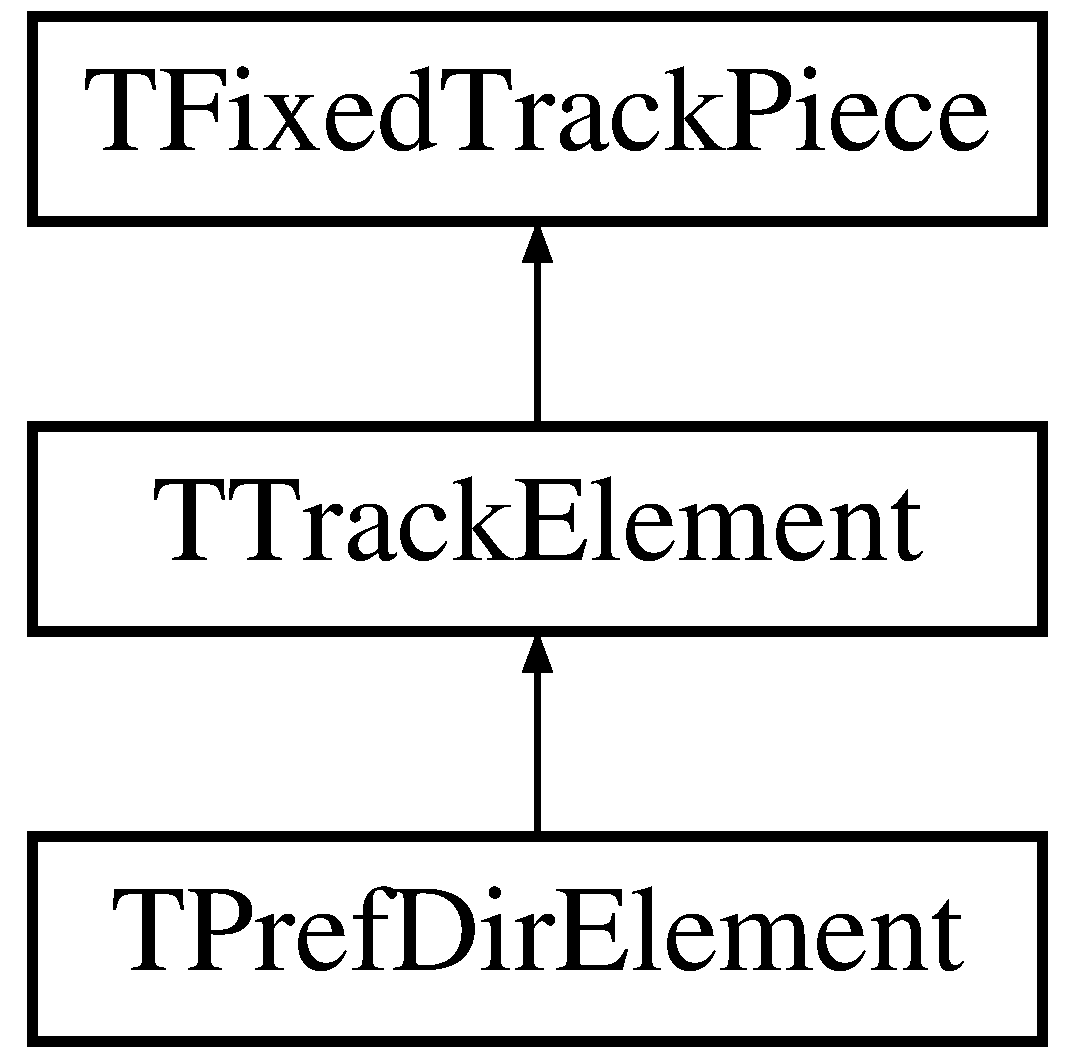
\includegraphics[height=3.000000cm]{class_t_track_element}
\end{center}
\end{figure}
\subsection*{Public Types}
\begin{DoxyCompactItemize}
\item 
\mbox{\Hypertarget{class_t_track_element_abbbcaeb3e062e962d53337965d4fcaad}\label{class_t_track_element_abbbcaeb3e062e962d53337965d4fcaad}} 
enum \{ {\bfseries Four\+Aspect}, 
{\bfseries Three\+Aspect}, 
{\bfseries Two\+Aspect}, 
{\bfseries Ground\+Signal}
 \}
\end{DoxyCompactItemize}
\subsection*{Public Member Functions}
\begin{DoxyCompactItemize}
\item 
\mbox{\hyperlink{class_t_track_element_a47b976d743e1d92e81ee807c410ef094}{T\+Track\+Element}} (\mbox{\hyperlink{class_t_fixed_track_piece}{T\+Fixed\+Track\+Piece}} Input)
\item 
\mbox{\hyperlink{class_t_track_element_a0f269bad77fe6988e0c2e0a542410d0e}{T\+Track\+Element}} ()
\item 
\mbox{\Hypertarget{class_t_track_element_aae268d9684a1de26e01dd6578b0f3527}\label{class_t_track_element_aae268d9684a1de26e01dd6578b0f3527}} 
bool \mbox{\hyperlink{class_t_track_element_aae268d9684a1de26e01dd6578b0f3527}{operator==}} (\mbox{\hyperlink{class_t_track_element}{T\+Track\+Element}} R\+H\+Element)
\begin{DoxyCompactList}\small\item\em equivalence operator \end{DoxyCompactList}\item 
bool \mbox{\hyperlink{class_t_track_element_ab8e14338f1059d834353d6c2264b80ee}{operator!=}} (\mbox{\hyperlink{class_t_track_element}{T\+Track\+Element}} R\+H\+Element)
\item 
\mbox{\Hypertarget{class_t_track_element_a100bff829c4dca820927affde4cb9e57}\label{class_t_track_element_a100bff829c4dca820927affde4cb9e57}} 
Ansi\+String \mbox{\hyperlink{class_t_track_element_a100bff829c4dca820927affde4cb9e57}{Log\+Track}} (int Caller) const
\begin{DoxyCompactList}\small\item\em Used to log track parameters for call stack logging. \end{DoxyCompactList}\item 
void \mbox{\hyperlink{class_t_track_element_a453377f8db5e108cb274464333e1100f}{Plot\+Variable\+Track\+Element}} (int Caller, \mbox{\hyperlink{class_t_display}{T\+Display}} $\ast$Disp) const
\end{DoxyCompactItemize}
\subsection*{Public Attributes}
\begin{DoxyCompactItemize}
\item 
Ansi\+String \mbox{\hyperlink{class_t_track_element_aa74717ece7b257122688b6f5855d6125}{Active\+Track\+Element\+Name}}
\item 
\mbox{\Hypertarget{class_t_track_element_ae780fef4d1277dfeeec0b770ae8b0919}\label{class_t_track_element_ae780fef4d1277dfeeec0b770ae8b0919}} 
Ansi\+String \mbox{\hyperlink{class_t_track_element_ae780fef4d1277dfeeec0b770ae8b0919}{Element\+ID}}
\begin{DoxyCompactList}\small\item\em the element identifier based on position in the railway \end{DoxyCompactList}\item 
Ansi\+String \mbox{\hyperlink{class_t_track_element_ae4aec8db868ce67f4ec275ce5a2249dc}{Location\+Name}}
\item 
\mbox{\Hypertarget{class_t_track_element_a7cde223e36c063fedde528797b3df77d}\label{class_t_track_element_a7cde223e36c063fedde528797b3df77d}} 
bool \mbox{\hyperlink{class_t_track_element_a7cde223e36c063fedde528797b3df77d}{Calling\+On\+Set}}
\begin{DoxyCompactList}\small\item\em Used for for signals only when a train is being called on -\/ used to plot the position lights. \end{DoxyCompactList}\item 
\mbox{\Hypertarget{class_t_track_element_a130d91923ac416757bb7e3f47806295a}\label{class_t_track_element_a130d91923ac416757bb7e3f47806295a}} 
bool \mbox{\hyperlink{class_t_track_element_a130d91923ac416757bb7e3f47806295a}{Temp\+Marker}}
\begin{DoxyCompactList}\small\item\em Utility marker for program use. \end{DoxyCompactList}\item 
\mbox{\Hypertarget{class_t_track_element_a1712299f9cb22bb7afbe54e5a781f8ec}\label{class_t_track_element_a1712299f9cb22bb7afbe54e5a781f8ec}} 
bool {\bfseries Temp\+Track\+Marker01}
\item 
\mbox{\Hypertarget{class_t_track_element_ab0d0c071e2a124e9143e5c7bc2009805}\label{class_t_track_element_ab0d0c071e2a124e9143e5c7bc2009805}} 
bool \mbox{\hyperlink{class_t_track_element_ab0d0c071e2a124e9143e5c7bc2009805}{Temp\+Track\+Marker23}}
\begin{DoxyCompactList}\small\item\em Utility markers for program use. \end{DoxyCompactList}\item 
int \mbox{\hyperlink{class_t_track_element_a16594caf5c9e6a35bd4120ad639b8cc2}{Attribute}}
\item 
\mbox{\Hypertarget{class_t_track_element_a9551c6d789485c121203be6d51e4781f}\label{class_t_track_element_a9551c6d789485c121203be6d51e4781f}} 
int \mbox{\hyperlink{class_t_track_element_a9551c6d789485c121203be6d51e4781f}{Conn}} \mbox{[}4\mbox{]}
\begin{DoxyCompactList}\small\item\em Connecting element position in Track\+Vector, set to -\/1 if no connecting link or if track not linked. \end{DoxyCompactList}\item 
\mbox{\Hypertarget{class_t_track_element_a93a9094a1833fced2891c012bc46a4ea}\label{class_t_track_element_a93a9094a1833fced2891c012bc46a4ea}} 
int \mbox{\hyperlink{class_t_track_element_a93a9094a1833fced2891c012bc46a4ea}{Conn\+Link\+Pos}} \mbox{[}4\mbox{]}
\begin{DoxyCompactList}\small\item\em Connecting element link position (i.\+e. array positions of the connecting element links, in same order as Link\mbox{[}4\mbox{]}) \end{DoxyCompactList}\item 
\mbox{\Hypertarget{class_t_track_element_a0d0e30d5e7b76d90fb737316d50efdd0}\label{class_t_track_element_a0d0e30d5e7b76d90fb737316d50efdd0}} 
int {\bfseries H\+Loc}
\item 
\mbox{\Hypertarget{class_t_track_element_a0d9a1c95d1c1aedd0ffec4d24772cfbc}\label{class_t_track_element_a0d9a1c95d1c1aedd0ffec4d24772cfbc}} 
int \mbox{\hyperlink{class_t_track_element_a0d9a1c95d1c1aedd0ffec4d24772cfbc}{V\+Loc}}
\begin{DoxyCompactList}\small\item\em The h \& v locations in the railway (top lh corner of the first build screen = 0,0) \end{DoxyCompactList}\item 
\mbox{\Hypertarget{class_t_track_element_a63978116296522c989ee9e4257988ce6}\label{class_t_track_element_a63978116296522c989ee9e4257988ce6}} 
int {\bfseries Length01}
\item 
\mbox{\Hypertarget{class_t_track_element_ad37f3272aa6ca0329b55e4ec383ec5d2}\label{class_t_track_element_ad37f3272aa6ca0329b55e4ec383ec5d2}} 
int {\bfseries Length23}
\item 
\mbox{\Hypertarget{class_t_track_element_aa58aa17b09e19894f83844b6a0d26b1c}\label{class_t_track_element_aa58aa17b09e19894f83844b6a0d26b1c}} 
int {\bfseries Speed\+Limit01}
\item 
int \mbox{\hyperlink{class_t_track_element_abd898b7031200a2f24c1315b52c965cd}{Speed\+Limit23}}
\item 
\mbox{\Hypertarget{class_t_track_element_a243af97a79009b237beb0cdd6f7db969}\label{class_t_track_element_a243af97a79009b237beb0cdd6f7db969}} 
int {\bfseries Station\+Entry\+Stop\+Link\+Pos1}
\item 
int \mbox{\hyperlink{class_t_track_element_af6b589b13c3b59adb3c493816316ffe1}{Station\+Entry\+Stop\+Link\+Pos2}}
\item 
\mbox{\Hypertarget{class_t_track_element_a5f6319bc1752da843be71f1024774ace}\label{class_t_track_element_a5f6319bc1752da843be71f1024774ace}} 
int {\bfseries Train\+I\+D\+On\+Element}
\item 
\mbox{\Hypertarget{class_t_track_element_a9751b1ee4085deff881cd8f39bbd293b}\label{class_t_track_element_a9751b1ee4085deff881cd8f39bbd293b}} 
int {\bfseries Train\+I\+D\+On\+Bridge\+Track\+Pos01}
\item 
int \mbox{\hyperlink{class_t_track_element_aa3d8b1fef605f7ef4e6b09360abbb528}{Train\+I\+D\+On\+Bridge\+Track\+Pos23}}
\item 
\mbox{\Hypertarget{class_t_track_element_a2742b1ba840a4e8895d074e00791c464}\label{class_t_track_element_a2742b1ba840a4e8895d074e00791c464}} 
enum T\+Track\+Element\+:: \{ ... \}  \mbox{\hyperlink{class_t_track_element_a2742b1ba840a4e8895d074e00791c464}{Sig\+Aspect}}
\begin{DoxyCompactList}\small\item\em added at version 0.\+6 \end{DoxyCompactList}\end{DoxyCompactItemize}


\subsection{Detailed Description}
Basic track elements as implemented in the overall railway layout. 

\subsection{Constructor \& Destructor Documentation}
\mbox{\Hypertarget{class_t_track_element_a47b976d743e1d92e81ee807c410ef094}\label{class_t_track_element_a47b976d743e1d92e81ee807c410ef094}} 
\index{T\+Track\+Element@{T\+Track\+Element}!T\+Track\+Element@{T\+Track\+Element}}
\index{T\+Track\+Element@{T\+Track\+Element}!T\+Track\+Element@{T\+Track\+Element}}
\subsubsection{\texorpdfstring{T\+Track\+Element()}{TTrackElement()}\hspace{0.1cm}{\footnotesize\ttfamily [1/2]}}
{\footnotesize\ttfamily T\+Track\+Element\+::\+T\+Track\+Element (\begin{DoxyParamCaption}\item[{\mbox{\hyperlink{class_t_fixed_track_piece}{T\+Fixed\+Track\+Piece}}}]{Input }\end{DoxyParamCaption})\hspace{0.3cm}{\ttfamily [inline]}}

Constructor for specific type of element

Use very high neg. numbers as \textquotesingle{}unset\textquotesingle{} values for H\+Loc \& V\+Loc initially as can go high negatively legitimately, build from existing T\+Track\+Piece with default values for extra members \mbox{\Hypertarget{class_t_track_element_a0f269bad77fe6988e0c2e0a542410d0e}\label{class_t_track_element_a0f269bad77fe6988e0c2e0a542410d0e}} 
\index{T\+Track\+Element@{T\+Track\+Element}!T\+Track\+Element@{T\+Track\+Element}}
\index{T\+Track\+Element@{T\+Track\+Element}!T\+Track\+Element@{T\+Track\+Element}}
\subsubsection{\texorpdfstring{T\+Track\+Element()}{TTrackElement()}\hspace{0.1cm}{\footnotesize\ttfamily [2/2]}}
{\footnotesize\ttfamily T\+Track\+Element\+::\+T\+Track\+Element (\begin{DoxyParamCaption}{ }\end{DoxyParamCaption})\hspace{0.3cm}{\ttfamily [inline]}}

Constructor for non-\/specific default element

Use high neg numbers for \textquotesingle{}unset\textquotesingle{} h \& v as can go high negatively legitimately 

\subsection{Member Function Documentation}
\mbox{\Hypertarget{class_t_track_element_ab8e14338f1059d834353d6c2264b80ee}\label{class_t_track_element_ab8e14338f1059d834353d6c2264b80ee}} 
\index{T\+Track\+Element@{T\+Track\+Element}!operator"!=@{operator"!=}}
\index{operator"!=@{operator"!=}!T\+Track\+Element@{T\+Track\+Element}}
\subsubsection{\texorpdfstring{operator"!=()}{operator!=()}}
{\footnotesize\ttfamily bool T\+Track\+Element\+::operator!= (\begin{DoxyParamCaption}\item[{\mbox{\hyperlink{class_t_track_element}{T\+Track\+Element}}}]{R\+H\+Element }\end{DoxyParamCaption})}

non-\/equivalence operator \mbox{\Hypertarget{class_t_track_element_a453377f8db5e108cb274464333e1100f}\label{class_t_track_element_a453377f8db5e108cb274464333e1100f}} 
\index{T\+Track\+Element@{T\+Track\+Element}!Plot\+Variable\+Track\+Element@{Plot\+Variable\+Track\+Element}}
\index{Plot\+Variable\+Track\+Element@{Plot\+Variable\+Track\+Element}!T\+Track\+Element@{T\+Track\+Element}}
\subsubsection{\texorpdfstring{Plot\+Variable\+Track\+Element()}{PlotVariableTrackElement()}}
{\footnotesize\ttfamily void T\+Track\+Element\+::\+Plot\+Variable\+Track\+Element (\begin{DoxyParamCaption}\item[{int}]{Caller,  }\item[{\mbox{\hyperlink{class_t_display}{T\+Display}} $\ast$}]{Disp }\end{DoxyParamCaption}) const}

Plot the element on the display

\textquotesingle{}variable\textquotesingle{} indicates that the element may be named and if so may be plotted striped or solid depending on whether the name has been set 

\subsection{Member Data Documentation}
\mbox{\Hypertarget{class_t_track_element_aa74717ece7b257122688b6f5855d6125}\label{class_t_track_element_aa74717ece7b257122688b6f5855d6125}} 
\index{T\+Track\+Element@{T\+Track\+Element}!Active\+Track\+Element\+Name@{Active\+Track\+Element\+Name}}
\index{Active\+Track\+Element\+Name@{Active\+Track\+Element\+Name}!T\+Track\+Element@{T\+Track\+Element}}
\subsubsection{\texorpdfstring{Active\+Track\+Element\+Name}{ActiveTrackElementName}}
{\footnotesize\ttfamily Ansi\+String T\+Track\+Element\+::\+Active\+Track\+Element\+Name}

Location name used either in the timetable or for a continuation (continuation names not used in timetable as trains can\textquotesingle{}t stop there). Only active track elements where there are platforms or non-\/station named locations have Active\+Track\+Element\+Names \mbox{\Hypertarget{class_t_track_element_a16594caf5c9e6a35bd4120ad639b8cc2}\label{class_t_track_element_a16594caf5c9e6a35bd4120ad639b8cc2}} 
\index{T\+Track\+Element@{T\+Track\+Element}!Attribute@{Attribute}}
\index{Attribute@{Attribute}!T\+Track\+Element@{T\+Track\+Element}}
\subsubsection{\texorpdfstring{Attribute}{Attribute}}
{\footnotesize\ttfamily int T\+Track\+Element\+::\+Attribute}

special variable used only for points \& signals, ignored otherwise points\+: 0=set to go straight, 1=set to diverge; where both legs diverge 0=set to left fork signals\+: 0=red; 1=yellow; 2=double yellow; 3 = green; Level crossing\+: 0 = raised barriers = closed to trains; 1 = lowered barriers = open to trains; 2 = changing state = closed to trains \mbox{\Hypertarget{class_t_track_element_ae4aec8db868ce67f4ec275ce5a2249dc}\label{class_t_track_element_ae4aec8db868ce67f4ec275ce5a2249dc}} 
\index{T\+Track\+Element@{T\+Track\+Element}!Location\+Name@{Location\+Name}}
\index{Location\+Name@{Location\+Name}!T\+Track\+Element@{T\+Track\+Element}}
\subsubsection{\texorpdfstring{Location\+Name}{LocationName}}
{\footnotesize\ttfamily Ansi\+String T\+Track\+Element\+::\+Location\+Name}

location name not used for timetabling, only for identification\+: platforms, non-\/station named locations, concourses and footbridges have Location\+Names \mbox{\Hypertarget{class_t_track_element_abd898b7031200a2f24c1315b52c965cd}\label{class_t_track_element_abd898b7031200a2f24c1315b52c965cd}} 
\index{T\+Track\+Element@{T\+Track\+Element}!Speed\+Limit23@{Speed\+Limit23}}
\index{Speed\+Limit23@{Speed\+Limit23}!T\+Track\+Element@{T\+Track\+Element}}
\subsubsection{\texorpdfstring{Speed\+Limit23}{SpeedLimit23}}
{\footnotesize\ttfamily int T\+Track\+Element\+::\+Speed\+Limit23}

Element lengths and speed limits, ...01 is for the track with link positions \mbox{[}0\mbox{]} and \mbox{[}1\mbox{]}, ...23 for \mbox{[}2\mbox{]} and \mbox{[}3\mbox{]}, set to -\/1 if not used (lengths in m \& speed limits in km/h) \mbox{\Hypertarget{class_t_track_element_af6b589b13c3b59adb3c493816316ffe1}\label{class_t_track_element_af6b589b13c3b59adb3c493816316ffe1}} 
\index{T\+Track\+Element@{T\+Track\+Element}!Station\+Entry\+Stop\+Link\+Pos2@{Station\+Entry\+Stop\+Link\+Pos2}}
\index{Station\+Entry\+Stop\+Link\+Pos2@{Station\+Entry\+Stop\+Link\+Pos2}!T\+Track\+Element@{T\+Track\+Element}}
\subsubsection{\texorpdfstring{Station\+Entry\+Stop\+Link\+Pos2}{StationEntryStopLinkPos2}}
{\footnotesize\ttfamily int T\+Track\+Element\+::\+Station\+Entry\+Stop\+Link\+Pos2}

Used for track at platforms and non-\/station named locations to mark the train front element stop position, there are two for the two directions of travel, set to -\/1 if not used \mbox{\Hypertarget{class_t_track_element_aa3d8b1fef605f7ef4e6b09360abbb528}\label{class_t_track_element_aa3d8b1fef605f7ef4e6b09360abbb528}} 
\index{T\+Track\+Element@{T\+Track\+Element}!Train\+I\+D\+On\+Bridge\+Track\+Pos23@{Train\+I\+D\+On\+Bridge\+Track\+Pos23}}
\index{Train\+I\+D\+On\+Bridge\+Track\+Pos23@{Train\+I\+D\+On\+Bridge\+Track\+Pos23}!T\+Track\+Element@{T\+Track\+Element}}
\subsubsection{\texorpdfstring{Train\+I\+D\+On\+Bridge\+Track\+Pos23}{TrainIDOnBridgeTrackPos23}}
{\footnotesize\ttfamily int T\+Track\+Element\+::\+Train\+I\+D\+On\+Bridge\+Track\+Pos23}

Set to the Train\+ID value when a train is present on the element, bridges can have two trains present so the ...01 and ...23 values give the Train\+I\+Ds for track with link positions \mbox{[}0\mbox{]} \& \mbox{[}1\mbox{]}, and \mbox{[}2\mbox{]} \& \mbox{[}3\mbox{]} respectively 

The documentation for this class was generated from the following files\+:\begin{DoxyCompactItemize}
\item 
C\+:/\+Programming work/railway development after v2.\+2.\+0/Track\+Unit.\+h\item 
C\+:/\+Programming work/railway development after v2.\+2.\+0/Track\+Unit.\+cpp\end{DoxyCompactItemize}

\hypertarget{class_t_train}{}\section{T\+Train Class Reference}
\label{class_t_train}\index{T\+Train@{T\+Train}}


Collaboration diagram for T\+Train\+:\nopagebreak
\begin{figure}[H]
\begin{center}
\leavevmode
\includegraphics[height=550pt]{class_t_train__coll__graph}
\end{center}
\end{figure}
\subsection*{Public Member Functions}
\begin{DoxyCompactItemize}
\item 
\mbox{\Hypertarget{class_t_train_a2a2d78164c9dc1881b2c77526f04903f}\label{class_t_train_a2a2d78164c9dc1881b2c77526f04903f}} 
bool \mbox{\hyperlink{class_t_train_a2a2d78164c9dc1881b2c77526f04903f}{Stopped}} ()
\begin{DoxyCompactList}\small\item\em True if the train has stopped for any reason. \end{DoxyCompactList}\item 
bool \mbox{\hyperlink{class_t_train_aef32cd9a007874ab09ceeac907e7c88b}{Link\+Occupied}} (int Caller, int Track\+Vector\+Position, int Link\+Number)
\item 
\mbox{\Hypertarget{class_t_train_ae9d788d7bf536de1efe7a67ab5bb8dd7}\label{class_t_train_ae9d788d7bf536de1efe7a67ab5bb8dd7}} 
\mbox{\hyperlink{class_t_train_ae9d788d7bf536de1efe7a67ab5bb8dd7}{T\+Train}} (int Caller, int Rear\+Start\+Element\+In, int Rear\+Start\+Exit\+Pos\+In, Ansi\+String Input\+Code, int \mbox{\hyperlink{class_t_train_adae3a1fd82da0457a983a3ac41cdda3d}{Start\+Speed}}, int \mbox{\hyperlink{class_t_train_ab9dabc7092d31bc27b573e75ac74d0da}{Mass}}, double \mbox{\hyperlink{class_t_train_a0b9ba6ba25c153ba3142f63ec024ccde}{Max\+Running\+Speed}}, double \mbox{\hyperlink{class_t_train_a1cd5cd53f56a05bc4fde337e44bdd6d4}{Max\+Brake\+Rate}}, double \mbox{\hyperlink{class_t_train_a6940d3fe404390d1d345a80bde3f6bf9}{Power\+At\+Rail}}, T\+Train\+Mode \mbox{\hyperlink{class_t_train_a860f87857baefc44a4928311698055a8}{Train\+Mode}}, \mbox{\hyperlink{class_t_train_data_entry}{T\+Train\+Data\+Entry}} $\ast$\mbox{\hyperlink{class_t_train_a28a2217abf201b23fd8b3b92c12038b7}{Train\+Data\+Entry\+Ptr}}, int \mbox{\hyperlink{class_t_train_a459ae11b674cfdccb8872ef25c921fd9}{Repeat\+Number}}, int \mbox{\hyperlink{class_t_train_a8601120683e9bf4f26b0d1cba75ceed4}{Incremental\+Minutes}}, int \mbox{\hyperlink{class_t_train_a7390e5172ab0a5aa998df94953e43fba}{Incremental\+Digits}}, int \mbox{\hyperlink{class_t_train_ad11759e49fa6fcf8367090ef1db490b7}{Signaller\+Max\+Speed}})
\begin{DoxyCompactList}\small\item\em Constructor, sets listed member values. \end{DoxyCompactList}\end{DoxyCompactItemize}
\subsection*{Private Member Functions}
\begin{DoxyCompactItemize}
\item 
\mbox{\Hypertarget{class_t_train_a2e3e9fd7367a9333b7550b225d328d13}\label{class_t_train_a2e3e9fd7367a9333b7550b225d328d13}} 
bool \mbox{\hyperlink{class_t_train_a2e3e9fd7367a9333b7550b225d328d13}{Buffer\+At\+Exit}} (int Caller, int Element, int Exitpos) const
\begin{DoxyCompactList}\small\item\em True if Element is a buffer and Exitpos is the buffer end. \end{DoxyCompactList}\item 
\mbox{\Hypertarget{class_t_train_a4524b72ef62ef2c1375f58fac05929ee}\label{class_t_train_a4524b72ef62ef2c1375f58fac05929ee}} 
bool \mbox{\hyperlink{class_t_train_a4524b72ef62ef2c1375f58fac05929ee}{Calling\+On\+Allowed}} (int Caller)
\begin{DoxyCompactList}\small\item\em True if the train can be called on at its current position -\/ see detail in .cpp file. \end{DoxyCompactList}\item 
\mbox{\Hypertarget{class_t_train_a36b7b4901add145605ba1e540801b6cf}\label{class_t_train_a36b7b4901add145605ba1e540801b6cf}} 
bool \mbox{\hyperlink{class_t_train_a36b7b4901add145605ba1e540801b6cf}{Continuation\+Exit}} (int Caller, int Element, int Exitpos) const
\begin{DoxyCompactList}\small\item\em True if Element is a continuation and Exitpos is the continuation end. \end{DoxyCompactList}\item 
\mbox{\Hypertarget{class_t_train_a0a3a41dac70ba46da2f7f9fd03f2a63f}\label{class_t_train_a0a3a41dac70ba46da2f7f9fd03f2a63f}} 
bool \mbox{\hyperlink{class_t_train_a0a3a41dac70ba46da2f7f9fd03f2a63f}{Is\+Train\+I\+D\+On\+Bridge\+Track\+Pos01}} (int Caller, unsigned int Track\+Vector\+Position)
\begin{DoxyCompactList}\small\item\em True if train is on a bridge on trackpos 0 \& 1. \end{DoxyCompactList}\item 
\mbox{\Hypertarget{class_t_train_a6cbff3229246b7a156cd64a531aa60a6}\label{class_t_train_a6cbff3229246b7a156cd64a531aa60a6}} 
bool \mbox{\hyperlink{class_t_train_a6cbff3229246b7a156cd64a531aa60a6}{Is\+Train\+I\+D\+On\+Bridge\+Track\+Pos23}} (int Caller, unsigned int Track\+Vector\+Position)
\begin{DoxyCompactList}\small\item\em True if train is on a bridge on trackpos 2 \& 3. \end{DoxyCompactList}\item 
\mbox{\Hypertarget{class_t_train_a89e17b8d82633276576e365c980e718a}\label{class_t_train_a89e17b8d82633276576e365c980e718a}} 
bool \mbox{\hyperlink{class_t_train_a89e17b8d82633276576e365c980e718a}{Is\+Train\+Terminating}} (int Caller)
\begin{DoxyCompactList}\small\item\em True if train service terminates at its current location. \end{DoxyCompactList}\item 
bool \mbox{\hyperlink{class_t_train_ac2f3802b0d193d220ec6d19e2a6fc7ed}{Low\+Entry\+Value}} (int Entry\+Link) const
\item 
\mbox{\Hypertarget{class_t_train_ab4fefd748946d8530bca23a7699d0abc}\label{class_t_train_ab4fefd748946d8530bca23a7699d0abc}} 
bool \mbox{\hyperlink{class_t_train_ab4fefd748946d8530bca23a7699d0abc}{Train\+To\+Be\+Joined\+By\+Is\+Adjacent}} (int Caller, \mbox{\hyperlink{class_t_train}{T\+Train}} $\ast$\&Train\+To\+Be\+Joined\+By)
\begin{DoxyCompactList}\small\item\em True for a train waiting to be joined when the joining train is adjacent. \end{DoxyCompactList}\item 
\mbox{\Hypertarget{class_t_train_a23b7b40bba00cae3550bb1a30670c249}\label{class_t_train_a23b7b40bba00cae3550bb1a30670c249}} 
bool \mbox{\hyperlink{class_t_train_a23b7b40bba00cae3550bb1a30670c249}{Train\+To\+Join\+Is\+Adjacent}} (int Caller, \mbox{\hyperlink{class_t_train}{T\+Train}} $\ast$\&Train\+To\+Join)
\begin{DoxyCompactList}\small\item\em True for a train waiting to join another when the other train is adjacent. \end{DoxyCompactList}\item 
\mbox{\Hypertarget{class_t_train_ad7831e71f0c68933df4aea6661a77be5}\label{class_t_train_ad7831e71f0c68933df4aea6661a77be5}} 
Graphics\+::\+T\+Bitmap $\ast$ \mbox{\hyperlink{class_t_train_ad7831e71f0c68933df4aea6661a77be5}{Set\+One\+Graphic\+Code}} (char Code\+Char)
\begin{DoxyCompactList}\small\item\em Return a pointer to the graphic corresponding to the character \textquotesingle{}Code\+Vhar\textquotesingle{}. \end{DoxyCompactList}\item 
\mbox{\Hypertarget{class_t_train_a406c172a0ba96802ada1aa04d78948d0}\label{class_t_train_a406c172a0ba96802ada1aa04d78948d0}} 
void \mbox{\hyperlink{class_t_train_a406c172a0ba96802ada1aa04d78948d0}{Change\+Train\+Direction}} (int Caller)
\begin{DoxyCompactList}\small\item\em Reverses the direction of motion of the train. \end{DoxyCompactList}\item 
void \mbox{\hyperlink{class_t_train_a50997f7e8138a7e6a147fe3b5ad21b84}{Check\+And\+Cancel\+Route\+For\+Wrong\+End\+Entry}} (int Caller, int Element, int Entry\+Pos)
\item 
\mbox{\Hypertarget{class_t_train_ab9edf458753619f8cd25f0165484d26f}\label{class_t_train_ab9edf458753619f8cd25f0165484d26f}} 
void \mbox{\hyperlink{class_t_train_ab9edf458753619f8cd25f0165484d26f}{Finish\+Join}} (int Caller)
\begin{DoxyCompactList}\small\item\em Carry out the actions needed when a train is waiting to join another train. \end{DoxyCompactList}\item 
\mbox{\Hypertarget{class_t_train_ad666fb061d1da7c44a72ec963c2098aa}\label{class_t_train_ad666fb061d1da7c44a72ec963c2098aa}} 
void \mbox{\hyperlink{class_t_train_ad666fb061d1da7c44a72ec963c2098aa}{Front\+Train\+Split}} (int Caller)
\begin{DoxyCompactList}\small\item\em Carry out the actions needed when a train is to split from the front. \end{DoxyCompactList}\item 
void \mbox{\hyperlink{class_t_train_a0675ea1dede706d5b0dd52264496865a}{Get\+Lead\+Element}} (int Caller)
\item 
\mbox{\Hypertarget{class_t_train_aa973b7a0ecaef5077fd56398419f9104}\label{class_t_train_aa973b7a0ecaef5077fd56398419f9104}} 
void \mbox{\hyperlink{class_t_train_aa973b7a0ecaef5077fd56398419f9104}{Get\+Offset\+Values}} (int Caller, int \&H\+Offset, int \&\mbox{\hyperlink{class_t_train_a4c8b153a620229a3d9cc54f64ffa5f4a}{V\+Offset}}, int Link) const
\begin{DoxyCompactList}\small\item\em Sets H\+Offset \& V\+Offset (see above) for a single headcode character depending on the Link value. \end{DoxyCompactList}\item 
\mbox{\Hypertarget{class_t_train_a6c3479378d35f9041c38d80f03686b41}\label{class_t_train_a6c3479378d35f9041c38d80f03686b41}} 
void \mbox{\hyperlink{class_t_train_a6c3479378d35f9041c38d80f03686b41}{Joined\+By}} (int Caller)
\begin{DoxyCompactList}\small\item\em Carry out the actions needed when a train is waiting to be joined by another train. \end{DoxyCompactList}\item 
\mbox{\Hypertarget{class_t_train_a56fcfe4b9a3cef988bbeb4f4766372aa}\label{class_t_train_a56fcfe4b9a3cef988bbeb4f4766372aa}} 
void \mbox{\hyperlink{class_t_train_a56fcfe4b9a3cef988bbeb4f4766372aa}{New\+Shuttle\+From\+Non\+Repeat\+Service}} (int Caller)
\begin{DoxyCompactList}\small\item\em Carry out the actions needed when a new shuttle service is created from a non-\/repeating (F-\/nshs) service. \end{DoxyCompactList}\item 
\mbox{\Hypertarget{class_t_train_a75a2e9017b96e2a8f2a1edbd01c2cd68}\label{class_t_train_a75a2e9017b96e2a8f2a1edbd01c2cd68}} 
void \mbox{\hyperlink{class_t_train_a75a2e9017b96e2a8f2a1edbd01c2cd68}{New\+Train\+Service}} (int Caller)
\begin{DoxyCompactList}\small\item\em Carry out the actions needed when a train forms a new service (code Fns) \end{DoxyCompactList}\item 
void \mbox{\hyperlink{class_t_train_af92ae73f1be23475e7ae424306cd4866}{Pick\+Up\+Background\+Bitmap}} (int Caller, int H\+Offset, int \mbox{\hyperlink{class_t_train_a4c8b153a620229a3d9cc54f64ffa5f4a}{V\+Offset}}, int Element, int Entry\+Pos, Graphics\+::\+T\+Bitmap $\ast$Graphic\+Ptr) const
\item 
void \mbox{\hyperlink{class_t_train_aa21e18b3085773ca8351c446911611c1}{Plot\+Alternative\+Track\+Route\+Graphic}} (int Caller, unsigned int Lag\+Element, int Lag\+E\+Link\+Pos, int H\+Offset, int \mbox{\hyperlink{class_t_train_a4c8b153a620229a3d9cc54f64ffa5f4a}{V\+Offset}}, T\+Straddle Straddle\+Value)
\item 
\mbox{\Hypertarget{class_t_train_abb6bb7d2024ac59230cbaff2ec3ee999}\label{class_t_train_abb6bb7d2024ac59230cbaff2ec3ee999}} 
void \mbox{\hyperlink{class_t_train_abb6bb7d2024ac59230cbaff2ec3ee999}{Plot\+Background\+Graphic}} (int Caller, int Array\+Number, \mbox{\hyperlink{class_t_display}{T\+Display}} $\ast$Disp) const
\begin{DoxyCompactList}\small\item\em Replot the graphic pointed to by Background\+Ptr (see above) after a train has passed. \end{DoxyCompactList}\item 
\mbox{\Hypertarget{class_t_train_a247bd95a7c648367736b116f553f4e54}\label{class_t_train_a247bd95a7c648367736b116f553f4e54}} 
void \mbox{\hyperlink{class_t_train_a247bd95a7c648367736b116f553f4e54}{Plot\+Train\+Graphic}} (int Caller, int Array\+Number, \mbox{\hyperlink{class_t_display}{T\+Display}} $\ast$Disp)
\begin{DoxyCompactList}\small\item\em Plot the train\textquotesingle{}s headcode character corresponding to Array\+Number. \end{DoxyCompactList}\item 
\mbox{\Hypertarget{class_t_train_abfa6da75d034c737d53819e6edbfa3dc}\label{class_t_train_abfa6da75d034c737d53819e6edbfa3dc}} 
void \mbox{\hyperlink{class_t_train_abfa6da75d034c737d53819e6edbfa3dc}{Plot\+Train\+With\+New\+Background\+Colour}} (int Caller, T\+Color New\+Background\+Colour, \mbox{\hyperlink{class_t_display}{T\+Display}} $\ast$Disp)
\begin{DoxyCompactList}\small\item\em Changes the train\textquotesingle{}s background colour (e.\+g. to pale green if stopped at a station) \end{DoxyCompactList}\item 
\mbox{\Hypertarget{class_t_train_ad64c5823265b0c611c2e5f0613317aa5}\label{class_t_train_ad64c5823265b0c611c2e5f0613317aa5}} 
void \mbox{\hyperlink{class_t_train_ad64c5823265b0c611c2e5f0613317aa5}{Rear\+Train\+Split}} (int Caller)
\begin{DoxyCompactList}\small\item\em Carry out the actions needed when a train is to split from the rear. \end{DoxyCompactList}\item 
\mbox{\Hypertarget{class_t_train_abd68a68b5ce295ee01171615f3d2c7ec}\label{class_t_train_abd68a68b5ce295ee01171615f3d2c7ec}} 
void \mbox{\hyperlink{class_t_train_abd68a68b5ce295ee01171615f3d2c7ec}{Remain\+Here}} (int Caller)
\begin{DoxyCompactList}\small\item\em Sends the \textquotesingle{}train terminated\textquotesingle{} message to the performance log and sets Timetable\+Finished to true. \end{DoxyCompactList}\item 
void \mbox{\hyperlink{class_t_train_a8262f447ec811db7e524c7bb885226c5}{Repeat\+Shuttle\+Or\+New\+Non\+Repeat\+Service}} (int Caller)
\item 
void \mbox{\hyperlink{class_t_train_ac6f5cda912103fda4da31bdca611e4b5}{Repeat\+Shuttle\+Or\+Remain\+Here}} (int Caller)
\item 
void \mbox{\hyperlink{class_t_train_ace302d98b5685104d294869b161e20a0}{Reset\+Train\+Element\+ID}} (int Caller, unsigned int Track\+Vector\+Position, int Entry\+Pos)
\item 
void \mbox{\hyperlink{class_t_train_a594228489e522dfde0ffbe124cd27103}{Set\+Head\+Code\+Graphics}} (int Caller, Ansi\+String Code)
\item 
void \mbox{\hyperlink{class_t_train_a0e0ab54415645b04cbdeadd829d27898}{Set\+Train\+Element\+ID}} (int Caller, unsigned int Track\+Vector\+Position, int Entry\+Pos)
\item 
\mbox{\Hypertarget{class_t_train_af95a34f2334cb991841c24997d445ae3}\label{class_t_train_af95a34f2334cb991841c24997d445ae3}} 
bool \mbox{\hyperlink{class_t_train_af95a34f2334cb991841c24997d445ae3}{Has\+Train\+Gone}} ()
\begin{DoxyCompactList}\small\item\em Check whether the train has left the railway, so that it can be removed from the display at the next clock tick. \end{DoxyCompactList}\item 
\mbox{\Hypertarget{class_t_train_a221da69cd80d206a06f840f4cd463cf9}\label{class_t_train_a221da69cd80d206a06f840f4cd463cf9}} 
Ansi\+String \mbox{\hyperlink{class_t_train_a221da69cd80d206a06f840f4cd463cf9}{Floating\+Label\+Next\+String}} (int Caller, \mbox{\hyperlink{class_t_action_vector_entry}{T\+Action\+Vector\+Entry}} $\ast$Ptr)
\begin{DoxyCompactList}\small\item\em Used in the floating window to display the \textquotesingle{}Next\textquotesingle{} action. \end{DoxyCompactList}\item 
\mbox{\Hypertarget{class_t_train_a81bf61b47a2867f0c6901b1ea6f47177}\label{class_t_train_a81bf61b47a2867f0c6901b1ea6f47177}} 
Ansi\+String \mbox{\hyperlink{class_t_train_a81bf61b47a2867f0c6901b1ea6f47177}{Floating\+Timetable\+String}} (int Caller, \mbox{\hyperlink{class_t_action_vector_entry}{T\+Action\+Vector\+Entry}} $\ast$Ptr)
\begin{DoxyCompactList}\small\item\em Used in the floating window to display the timetable. \end{DoxyCompactList}\item 
\mbox{\Hypertarget{class_t_train_a63b0884e315178879369c82ee7fd2cb8}\label{class_t_train_a63b0884e315178879369c82ee7fd2cb8}} 
Ansi\+String \mbox{\hyperlink{class_t_train_a63b0884e315178879369c82ee7fd2cb8}{Get\+Train\+Head\+Code}} (int Caller)
\begin{DoxyCompactList}\small\item\em Returns the train headcode, taking account of the Repeat\+Number. \end{DoxyCompactList}\item 
\mbox{\Hypertarget{class_t_train_a659e6bf818f0cfac38728d4748408ee6}\label{class_t_train_a659e6bf818f0cfac38728d4748408ee6}} 
bool \mbox{\hyperlink{class_t_train_a659e6bf818f0cfac38728d4748408ee6}{Able\+To\+Move}} (int Caller)
\begin{DoxyCompactList}\small\item\em Indicates that a train is not prevented from moving -\/ used to allow appropriate popup menu options when under signaller control. \end{DoxyCompactList}\item 
\mbox{\Hypertarget{class_t_train_ab4f992b2aeb186f8d23879d9405296a3}\label{class_t_train_ab4f992b2aeb186f8d23879d9405296a3}} 
bool \mbox{\hyperlink{class_t_train_ab4f992b2aeb186f8d23879d9405296a3}{Able\+To\+Move\+But\+For\+Signal}} (int Caller)
\begin{DoxyCompactList}\small\item\em Indicates that a train is only prevented from moving by a signal -\/ used to allow appropriate popup menu options when under signaller control. \end{DoxyCompactList}\item 
bool \mbox{\hyperlink{class_t_train_aeed1f50d8a4f76d7d77991d276758570}{Clear\+To\+Next\+Signal}} (int Caller)
\item 
\mbox{\Hypertarget{class_t_train_a935bb43db57a3f2b635be9dfc6a7988b}\label{class_t_train_a935bb43db57a3f2b635be9dfc6a7988b}} 
bool \mbox{\hyperlink{class_t_train_a935bb43db57a3f2b635be9dfc6a7988b}{Train\+At\+Location}} (int Caller, Ansi\+String \&Location\+Name)
\begin{DoxyCompactList}\small\item\em True when the train is stopped at a timetabled location. \end{DoxyCompactList}\item 
int \mbox{\hyperlink{class_t_train_a7a54125a3a5052cb25e17014075a686b}{Name\+In\+Timetable\+Before\+C\+DT}} (int Caller, Ansi\+String Name, bool \&Stop)
\item 
T\+Date\+Time \mbox{\hyperlink{class_t_train_ad249f34f6862e604b8e141d1b25fe57d}{Get\+Train\+Time}} (int Caller, T\+Date\+Time Time)
\item 
void \mbox{\hyperlink{class_t_train_afd5d7ea375b8a878c31d81841acad159}{Delete\+Train}} (int Caller)
\item 
\mbox{\Hypertarget{class_t_train_a23c65e7f2b2130ae87811f70afb6d5bf}\label{class_t_train_a23c65e7f2b2130ae87811f70afb6d5bf}} 
void \mbox{\hyperlink{class_t_train_a23c65e7f2b2130ae87811f70afb6d5bf}{Load\+One\+Session\+Train}} (int Caller, std\+::ifstream \&In\+File)
\begin{DoxyCompactList}\small\item\em Create one train with relevant member values from the sesion file. \end{DoxyCompactList}\item 
void \mbox{\hyperlink{class_t_train_a493ab1c185d29bf28ec8fded2356e9fc}{Log\+Action}} (int Caller, Ansi\+String \mbox{\hyperlink{class_t_train_a68f4b62f3405f80d58f33519392ab37e}{Head\+Code}}, Ansi\+String Other\+Head\+Code, T\+Action\+Type Action\+Type, Ansi\+String Location\+Name, T\+Date\+Time Timetable\+Non\+Repeat\+Time, bool Warning)
\item 
\mbox{\Hypertarget{class_t_train_a43cd691f12297c4c13a19791329dd627}\label{class_t_train_a43cd691f12297c4c13a19791329dd627}} 
void \mbox{\hyperlink{class_t_train_a43cd691f12297c4c13a19791329dd627}{Plot\+Start\+Position}} (int Caller)
\begin{DoxyCompactList}\small\item\em Plots the train and sets up all relevant members for a new train when it is introduced into the railway. \end{DoxyCompactList}\item 
\mbox{\Hypertarget{class_t_train_a5fdef825574f0e546ab25169e9f8445d}\label{class_t_train_a5fdef825574f0e546ab25169e9f8445d}} 
void \mbox{\hyperlink{class_t_train_a5fdef825574f0e546ab25169e9f8445d}{Plot\+Train}} (int Caller, \mbox{\hyperlink{class_t_display}{T\+Display}} $\ast$Disp)
\begin{DoxyCompactList}\small\item\em Plots the train on the display in normal (zoomed-\/in) mode. \end{DoxyCompactList}\item 
\mbox{\Hypertarget{class_t_train_aa3f3a500264ddca35c7fee35f22ffa1e}\label{class_t_train_aa3f3a500264ddca35c7fee35f22ffa1e}} 
void \mbox{\hyperlink{class_t_train_aa3f3a500264ddca35c7fee35f22ffa1e}{Plot\+Train\+In\+Zoom\+Out\+Mode}} (int Caller, bool Flash)
\begin{DoxyCompactList}\small\item\em Plots the train on screen in zoomed-\/out mode, state of \textquotesingle{}Flash\textquotesingle{} determines whether the flashing trains are plotted or not. \end{DoxyCompactList}\item 
\mbox{\Hypertarget{class_t_train_ac414e9e4fd7e25c11e09678dd4dc7944}\label{class_t_train_ac414e9e4fd7e25c11e09678dd4dc7944}} 
void \mbox{\hyperlink{class_t_train_ac414e9e4fd7e25c11e09678dd4dc7944}{Save\+One\+Session\+Train}} (int Caller, std\+::ofstream \&Out\+File)
\begin{DoxyCompactList}\small\item\em Data for a single train is saved to a session file. \end{DoxyCompactList}\item 
\mbox{\Hypertarget{class_t_train_a29ad7cb992931e1e8922941fc49e2e74}\label{class_t_train_a29ad7cb992931e1e8922941fc49e2e74}} 
void \mbox{\hyperlink{class_t_train_a29ad7cb992931e1e8922941fc49e2e74}{Send\+Missed\+Action\+Logs}} (int Caller, int Inc\+Num, \mbox{\hyperlink{class_t_action_vector_entry}{T\+Action\+Vector\+Entry}} $\ast$Ptr)
\begin{DoxyCompactList}\small\item\em Missed actions (see Name\+In\+Timetable\+Before\+C\+DT above) sent to the performance log and performance file. \end{DoxyCompactList}\item 
\mbox{\Hypertarget{class_t_train_aaa6289d279b229d05963f8b3a35d53e9}\label{class_t_train_aaa6289d279b229d05963f8b3a35d53e9}} 
void \mbox{\hyperlink{class_t_train_aaa6289d279b229d05963f8b3a35d53e9}{Set\+Train\+Movement\+Values}} (int Caller, int Track\+Vector\+Position, int Entry\+Pos)
\begin{DoxyCompactList}\small\item\em Calculates train speeds and times for the element that the train is about to enter. \end{DoxyCompactList}\item 
\mbox{\Hypertarget{class_t_train_affbb94aa088370056f8ca8c45a1fdd48}\label{class_t_train_affbb94aa088370056f8ca8c45a1fdd48}} 
void \mbox{\hyperlink{class_t_train_affbb94aa088370056f8ca8c45a1fdd48}{Signaller\+Change\+Train\+Direction}} (int Caller)
\begin{DoxyCompactList}\small\item\em Unplots \& replots train, which checks for facing signal and sets Stopped\+At\+Signal if req\textquotesingle{}d. \end{DoxyCompactList}\item 
\mbox{\Hypertarget{class_t_train_a4978a3050ca943076eb6cbd03eeee1d4}\label{class_t_train_a4978a3050ca943076eb6cbd03eeee1d4}} 
void \mbox{\hyperlink{class_t_train_a4978a3050ca943076eb6cbd03eeee1d4}{Unplot\+Train}} (int Caller)
\begin{DoxyCompactList}\small\item\em Unplot train from screen in zoomed-\/in mode. \end{DoxyCompactList}\item 
\mbox{\Hypertarget{class_t_train_a439d2809c762a0981908a3b8a49520f2}\label{class_t_train_a439d2809c762a0981908a3b8a49520f2}} 
void \mbox{\hyperlink{class_t_train_a439d2809c762a0981908a3b8a49520f2}{Unplot\+Train\+In\+Zoom\+Out\+Mode}} (int Caller)
\begin{DoxyCompactList}\small\item\em Unplot train from screen in zoomed-\/out mode. \end{DoxyCompactList}\item 
\mbox{\Hypertarget{class_t_train_a89ad640ecf8f5163c40727b4e28575fc}\label{class_t_train_a89ad640ecf8f5163c40727b4e28575fc}} 
void \mbox{\hyperlink{class_t_train_a89ad640ecf8f5163c40727b4e28575fc}{Update\+Train}} (int Caller)
\begin{DoxyCompactList}\small\item\em Major function called at each clock tick for each train \& handles all train movement \& associated actions. \end{DoxyCompactList}\item 
void \mbox{\hyperlink{class_t_train_a86107a63225b0500b29e049f13545fff}{Write\+Train\+To\+Image}} (int Caller, Graphics\+::\+T\+Bitmap $\ast$Bitmap)
\end{DoxyCompactItemize}
\subsection*{Static Private Member Functions}
\begin{DoxyCompactItemize}
\item 
static bool \mbox{\hyperlink{class_t_train_aad716bab6f8f4aa6dd49f35130d28dd9}{Check\+One\+Session\+Train}} (std\+::ifstream \&In\+File)
\end{DoxyCompactItemize}
\subsection*{Private Attributes}
\begin{DoxyCompactItemize}
\item 
\mbox{\Hypertarget{class_t_train_abb385030108fe96cdcd550b2aa2072a7}\label{class_t_train_abb385030108fe96cdcd550b2aa2072a7}} 
friend {\bfseries T\+Train\+Controller}
\item 
\mbox{\Hypertarget{class_t_train_a0dd5144abd7dbc49a714d6c2e4cc1851}\label{class_t_train_a0dd5144abd7dbc49a714d6c2e4cc1851}} 
friend {\bfseries T\+Interface}
\item 
\mbox{\Hypertarget{class_t_train_a68f4b62f3405f80d58f33519392ab37e}\label{class_t_train_a68f4b62f3405f80d58f33519392ab37e}} 
Ansi\+String \mbox{\hyperlink{class_t_train_a68f4b62f3405f80d58f33519392ab37e}{Head\+Code}}
\begin{DoxyCompactList}\small\item\em needs own Head\+Code because repeat entries will differ from Train\+Data\+Entry.\+Head\+Code \end{DoxyCompactList}\item 
\mbox{\Hypertarget{class_t_train_a8f90e7446fd72ae99641a7ca9ee76ab6}\label{class_t_train_a8f90e7446fd72ae99641a7ca9ee76ab6}} 
bool \mbox{\hyperlink{class_t_train_a8f90e7446fd72ae99641a7ca9ee76ab6}{Hold\+At\+Location\+In\+T\+T\+Mode}}
\begin{DoxyCompactList}\small\item\em true if actions are needed before train departs \end{DoxyCompactList}\item 
\mbox{\Hypertarget{class_t_train_a4bfd087e177535b7e3086393c09e40a6}\label{class_t_train_a4bfd087e177535b7e3086393c09e40a6}} 
bool \mbox{\hyperlink{class_t_train_a4bfd087e177535b7e3086393c09e40a6}{Time\+Time\+Loc\+Arrived}}
\begin{DoxyCompactList}\small\item\em indicates whether has arrived (true) or not when Action\+Vector\+Entry\+Ptr-\/$>$Format\+Type == Time\+Time\+Loc \end{DoxyCompactList}\item 
\mbox{\Hypertarget{class_t_train_a52721f222fff0b6e08fffe94d693ac65}\label{class_t_train_a52721f222fff0b6e08fffe94d693ac65}} 
bool \mbox{\hyperlink{class_t_train_a52721f222fff0b6e08fffe94d693ac65}{Remain\+Here\+Log\+Not\+Sent}}
\begin{DoxyCompactList}\small\item\em flag to prevent repeated logs, new at v1.\+2.\+0 \end{DoxyCompactList}\item 
\mbox{\Hypertarget{class_t_train_a7390e5172ab0a5aa998df94953e43fba}\label{class_t_train_a7390e5172ab0a5aa998df94953e43fba}} 
int \mbox{\hyperlink{class_t_train_a7390e5172ab0a5aa998df94953e43fba}{Incremental\+Digits}}
\begin{DoxyCompactList}\small\item\em the number of digits to increment by in repeat entries \end{DoxyCompactList}\item 
\mbox{\Hypertarget{class_t_train_a8601120683e9bf4f26b0d1cba75ceed4}\label{class_t_train_a8601120683e9bf4f26b0d1cba75ceed4}} 
int \mbox{\hyperlink{class_t_train_a8601120683e9bf4f26b0d1cba75ceed4}{Incremental\+Minutes}}
\begin{DoxyCompactList}\small\item\em the number of minutes to increment by in repeat entries \end{DoxyCompactList}\item 
\mbox{\Hypertarget{class_t_train_a17d0d896f438220698e0b2b47e5112da}\label{class_t_train_a17d0d896f438220698e0b2b47e5112da}} 
int \mbox{\hyperlink{class_t_train_a17d0d896f438220698e0b2b47e5112da}{Rear\+Start\+Element}}
\begin{DoxyCompactList}\small\item\em start Track\+Vector\+Position element for rear of train \end{DoxyCompactList}\item 
\mbox{\Hypertarget{class_t_train_a469298d2fbbd846e2a62e7a04cfedc34}\label{class_t_train_a469298d2fbbd846e2a62e7a04cfedc34}} 
int \mbox{\hyperlink{class_t_train_a469298d2fbbd846e2a62e7a04cfedc34}{Rear\+Start\+Exit\+Pos}}
\begin{DoxyCompactList}\small\item\em the Link\+Pos value for the rear starting element (i.\+e. links to the front starting element) \end{DoxyCompactList}\item 
\mbox{\Hypertarget{class_t_train_a459ae11b674cfdccb8872ef25c921fd9}\label{class_t_train_a459ae11b674cfdccb8872ef25c921fd9}} 
int \mbox{\hyperlink{class_t_train_a459ae11b674cfdccb8872ef25c921fd9}{Repeat\+Number}}
\begin{DoxyCompactList}\small\item\em indicates which of the repeating services this train represents (0 = first service) \end{DoxyCompactList}\item 
\mbox{\Hypertarget{class_t_train_ad11759e49fa6fcf8367090ef1db490b7}\label{class_t_train_ad11759e49fa6fcf8367090ef1db490b7}} 
int \mbox{\hyperlink{class_t_train_ad11759e49fa6fcf8367090ef1db490b7}{Signaller\+Max\+Speed}}
\begin{DoxyCompactList}\small\item\em maximum train speed under signaller control (in km/h) \end{DoxyCompactList}\item 
\mbox{\Hypertarget{class_t_train_adae3a1fd82da0457a983a3ac41cdda3d}\label{class_t_train_adae3a1fd82da0457a983a3ac41cdda3d}} 
int \mbox{\hyperlink{class_t_train_adae3a1fd82da0457a983a3ac41cdda3d}{Start\+Speed}}
\begin{DoxyCompactList}\small\item\em the speed of the train when introduced into the railway (in km/h) \end{DoxyCompactList}\item 
\mbox{\Hypertarget{class_t_train_a28a2217abf201b23fd8b3b92c12038b7}\label{class_t_train_a28a2217abf201b23fd8b3b92c12038b7}} 
\mbox{\hyperlink{class_t_train_data_entry}{T\+Train\+Data\+Entry}} $\ast$ \mbox{\hyperlink{class_t_train_a28a2217abf201b23fd8b3b92c12038b7}{Train\+Data\+Entry\+Ptr}}
\begin{DoxyCompactList}\small\item\em points to the current position in the timetable\textquotesingle{}s Train\+Data\+Vector \end{DoxyCompactList}\item 
\mbox{\Hypertarget{class_t_train_a1caacc95f3c31b0d6f71704eeee44a00}\label{class_t_train_a1caacc95f3c31b0d6f71704eeee44a00}} 
\mbox{\hyperlink{class_t_action_vector_entry}{T\+Action\+Vector\+Entry}} $\ast$ \mbox{\hyperlink{class_t_train_a1caacc95f3c31b0d6f71704eeee44a00}{Action\+Vector\+Entry\+Ptr}}
\begin{DoxyCompactList}\small\item\em points to the current position in the Action\+Vector (a member of the \mbox{\hyperlink{class_t_train_data_entry}{T\+Train\+Data\+Entry}} class) \end{DoxyCompactList}\item 
bool \mbox{\hyperlink{class_t_train_a8c94580b79a8ad1ad0fce51f0abba822}{Allowed\+To\+Pass\+Red\+Signal}}
\item 
\mbox{\Hypertarget{class_t_train_a33f0f08a95cc392557392d02e293c7c3}\label{class_t_train_a33f0f08a95cc392557392d02e293c7c3}} 
bool \mbox{\hyperlink{class_t_train_a33f0f08a95cc392557392d02e293c7c3}{Being\+Called\+On}}
\begin{DoxyCompactList}\small\item\em in course of being called on to a station \end{DoxyCompactList}\item 
bool \mbox{\hyperlink{class_t_train_a60a3a9bebf64411f5d200682575a69ee}{Buffer\+Zoom\+Out\+Flash\+Required}}
\item 
\mbox{\Hypertarget{class_t_train_a5a658cdc377c3f4d65af6839614e7cb1}\label{class_t_train_a5a658cdc377c3f4d65af6839614e7cb1}} 
bool \mbox{\hyperlink{class_t_train_a5a658cdc377c3f4d65af6839614e7cb1}{Calling\+On\+Flag}}
\begin{DoxyCompactList}\small\item\em calling on permitted \end{DoxyCompactList}\item 
bool \mbox{\hyperlink{class_t_train_ab4f3876cb58a6160c2f1cd7a7eb3f234}{Departure\+Time\+Set}}
\item 
bool \mbox{\hyperlink{class_t_train_a638de0cfb04b13fb28edd5e61d2d628f}{First\+Half\+Move}}
\item 
bool \mbox{\hyperlink{class_t_train_a843a31af1c4faec4d71a61d32d6f4510}{Joined\+Other\+Train\+Flag}}
\item 
bool \mbox{\hyperlink{class_t_train_a1b53d5506e8a5bdfd55286ae2dc2d3f2}{Last\+Action\+Delay\+Flag}}
\item 
bool \mbox{\hyperlink{class_t_train_ac1ce3c1b548c1e4199d211b5fcd9763e}{Leaving\+Under\+Sig\+Control\+At\+Continuation}}
\item 
bool \mbox{\hyperlink{class_t_train_a36dc9bd48fb78d4257fe117908829dd7}{One\+Length\+Accel\+Decel}}
\item 
\mbox{\Hypertarget{class_t_train_a4cd38ef44706b5ae6bf0c934e58b4b93}\label{class_t_train_a4cd38ef44706b5ae6bf0c934e58b4b93}} 
bool \mbox{\hyperlink{class_t_train_a4cd38ef44706b5ae6bf0c934e58b4b93}{Signaller\+Removed}}
\begin{DoxyCompactList}\small\item\em set when removed under signaller control to force a removal from the display at the next clock tick \end{DoxyCompactList}\item 
\mbox{\Hypertarget{class_t_train_a559e8f1636c83d03463d6c901ae39567}\label{class_t_train_a559e8f1636c83d03463d6c901ae39567}} 
bool \mbox{\hyperlink{class_t_train_a559e8f1636c83d03463d6c901ae39567}{Signaller\+Stopping\+Flag}}
\begin{DoxyCompactList}\small\item\em set when the signaller stop command has been given \end{DoxyCompactList}\item 
\mbox{\Hypertarget{class_t_train_a0f044ad19728cee6dd0b6baadec4648b}\label{class_t_train_a0f044ad19728cee6dd0b6baadec4648b}} 
bool \mbox{\hyperlink{class_t_train_a0f044ad19728cee6dd0b6baadec4648b}{Step\+Forward\+Flag}}
\begin{DoxyCompactList}\small\item\em set when the signaller command to step forward one element has been given \end{DoxyCompactList}\item 
\mbox{\Hypertarget{class_t_train_aa714e9f320349edfe76fc9ac3ae3e20a}\label{class_t_train_aa714e9f320349edfe76fc9ac3ae3e20a}} 
bool \mbox{\hyperlink{class_t_train_aa714e9f320349edfe76fc9ac3ae3e20a}{Terminated\+Message\+Sent}}
\begin{DoxyCompactList}\small\item\em set when a \textquotesingle{}train terminated\textquotesingle{} message has been logged, to prevent its being logged more than once \end{DoxyCompactList}\item 
\mbox{\Hypertarget{class_t_train_a9e3744afb10713ef0b88f6fabb120236}\label{class_t_train_a9e3744afb10713ef0b88f6fabb120236}} 
bool \mbox{\hyperlink{class_t_train_a9e3744afb10713ef0b88f6fabb120236}{Timetable\+Finished}}
\begin{DoxyCompactList}\small\item\em set when there are no more timetable actions \end{DoxyCompactList}\item 
\mbox{\Hypertarget{class_t_train_a49612fd01b9450008b99d9fd66ac7583}\label{class_t_train_a49612fd01b9450008b99d9fd66ac7583}} 
double \mbox{\hyperlink{class_t_train_a49612fd01b9450008b99d9fd66ac7583}{A\+Value}}
\begin{DoxyCompactList}\small\item\em this is a useful shorthand value in calculating speeds and transit times in Set\+Train\+Movement\+Values \end{DoxyCompactList}\item 
\mbox{\Hypertarget{class_t_train_ae132daaee23376980818479528f27e2f}\label{class_t_train_ae132daaee23376980818479528f27e2f}} 
double \mbox{\hyperlink{class_t_train_ae132daaee23376980818479528f27e2f}{Entry\+Speed}}
\begin{DoxyCompactList}\small\item\em speed at which the train enters the next element \end{DoxyCompactList}\item 
\mbox{\Hypertarget{class_t_train_a05c926d79cbda85036d8d746131c3aef}\label{class_t_train_a05c926d79cbda85036d8d746131c3aef}} 
double \mbox{\hyperlink{class_t_train_a05c926d79cbda85036d8d746131c3aef}{Exit\+Speed\+Half}}
\begin{DoxyCompactList}\small\item\em speed when half way into the next element \end{DoxyCompactList}\item 
\mbox{\Hypertarget{class_t_train_ab3de27e27b474c1f2d224f73735fc1c2}\label{class_t_train_ab3de27e27b474c1f2d224f73735fc1c2}} 
double \mbox{\hyperlink{class_t_train_ab3de27e27b474c1f2d224f73735fc1c2}{Exit\+Speed\+Full}}
\begin{DoxyCompactList}\small\item\em speed when leaving the next element \end{DoxyCompactList}\item 
\mbox{\Hypertarget{class_t_train_adc5921a57f31d66e9b22f040717716d4}\label{class_t_train_adc5921a57f31d66e9b22f040717716d4}} 
double \mbox{\hyperlink{class_t_train_adc5921a57f31d66e9b22f040717716d4}{Timetable\+Max\+Running\+Speed}}
\begin{DoxyCompactList}\small\item\em the maximum train running speed when in timetable mode (see int Signaller\+Max\+Speed for signaller control) \end{DoxyCompactList}\item 
\mbox{\Hypertarget{class_t_train_a0b9ba6ba25c153ba3142f63ec024ccde}\label{class_t_train_a0b9ba6ba25c153ba3142f63ec024ccde}} 
double \mbox{\hyperlink{class_t_train_a0b9ba6ba25c153ba3142f63ec024ccde}{Max\+Running\+Speed}}
\begin{DoxyCompactList}\small\item\em the current maximum train running speed \end{DoxyCompactList}\item 
\mbox{\Hypertarget{class_t_train_ab0dc5c73f19ad8ef811f4464dfb5fc94}\label{class_t_train_ab0dc5c73f19ad8ef811f4464dfb5fc94}} 
double \mbox{\hyperlink{class_t_train_ab0dc5c73f19ad8ef811f4464dfb5fc94}{Max\+Exit\+Speed}}
\begin{DoxyCompactList}\small\item\em the maximum speed that the train can exit the next element \end{DoxyCompactList}\item 
\mbox{\Hypertarget{class_t_train_a1cd5cd53f56a05bc4fde337e44bdd6d4}\label{class_t_train_a1cd5cd53f56a05bc4fde337e44bdd6d4}} 
double \mbox{\hyperlink{class_t_train_a1cd5cd53f56a05bc4fde337e44bdd6d4}{Max\+Brake\+Rate}}
\begin{DoxyCompactList}\small\item\em the maximum brake rate that the train can achieve \end{DoxyCompactList}\item 
\mbox{\Hypertarget{class_t_train_afc10d4584267d8f4f05e9faa0a633a6e}\label{class_t_train_afc10d4584267d8f4f05e9faa0a633a6e}} 
double \mbox{\hyperlink{class_t_train_afc10d4584267d8f4f05e9faa0a633a6e}{Brake\+Rate}}
\begin{DoxyCompactList}\small\item\em the current train brake rate \end{DoxyCompactList}\item 
\mbox{\Hypertarget{class_t_train_a449a378257b8b3a3a2b3df40d0cca928}\label{class_t_train_a449a378257b8b3a3a2b3df40d0cca928}} 
double \mbox{\hyperlink{class_t_train_a449a378257b8b3a3a2b3df40d0cca928}{Signaller\+Stop\+Brake\+Rate}}
\begin{DoxyCompactList}\small\item\em the train brake rate when stopping under signaller control \end{DoxyCompactList}\item 
\mbox{\Hypertarget{class_t_train_a6940d3fe404390d1d345a80bde3f6bf9}\label{class_t_train_a6940d3fe404390d1d345a80bde3f6bf9}} 
double \mbox{\hyperlink{class_t_train_a6940d3fe404390d1d345a80bde3f6bf9}{Power\+At\+Rail}}
\begin{DoxyCompactList}\small\item\em in Watts (taken as 80\% of the train\textquotesingle{}s Gross Power, i.\+e. that entered by the user) \end{DoxyCompactList}\item 
\mbox{\Hypertarget{class_t_train_aa9d994b88696a8680438b109dccfd679}\label{class_t_train_aa9d994b88696a8680438b109dccfd679}} 
int {\bfseries Front\+Element\+Speed\+Limit}
\item 
\mbox{\Hypertarget{class_t_train_aac3a242d9fee653d2dca155d0279cc83}\label{class_t_train_aac3a242d9fee653d2dca155d0279cc83}} 
int \mbox{\hyperlink{class_t_train_aac3a242d9fee653d2dca155d0279cc83}{Front\+Element\+Length}}
\begin{DoxyCompactList}\small\item\em values associated with the element immediately in front of the train (speed in km/h, length in m) \end{DoxyCompactList}\item 
\mbox{\Hypertarget{class_t_train_ab9dabc7092d31bc27b573e75ac74d0da}\label{class_t_train_ab9dabc7092d31bc27b573e75ac74d0da}} 
int \mbox{\hyperlink{class_t_train_ab9dabc7092d31bc27b573e75ac74d0da}{Mass}}
\begin{DoxyCompactList}\small\item\em in kg \end{DoxyCompactList}\item 
int \mbox{\hyperlink{class_t_train_ae57749c241ad7256c6f628faf1168ce7}{Update\+Counter}}
\begin{DoxyCompactList}\small\item\em after a failure message has already been given (doesn\textquotesingle{}t need to stay failed as signaller can manoeuvre it to a better location) \end{DoxyCompactList}\item 
\mbox{\Hypertarget{class_t_train_a6baa340127335e185e91f150ab93986f}\label{class_t_train_a6baa340127335e185e91f150ab93986f}} 
T\+Date\+Time {\bfseries Entry\+Time}
\item 
\mbox{\Hypertarget{class_t_train_a8e1741c26fe9887f84f1491d16e52f0d}\label{class_t_train_a8e1741c26fe9887f84f1491d16e52f0d}} 
T\+Date\+Time {\bfseries Exit\+Time\+Half}
\item 
\mbox{\Hypertarget{class_t_train_abe007893bd4ba34a70260734107d9cc4}\label{class_t_train_abe007893bd4ba34a70260734107d9cc4}} 
T\+Date\+Time \mbox{\hyperlink{class_t_train_abe007893bd4ba34a70260734107d9cc4}{Exit\+Time\+Full}}
\begin{DoxyCompactList}\small\item\em times used in Set\+Train\+Movement\+Values corresponding to the next element the train runs on \end{DoxyCompactList}\item 
\mbox{\Hypertarget{class_t_train_a284962532ed0464d56031f46bae2354a}\label{class_t_train_a284962532ed0464d56031f46bae2354a}} 
T\+Date\+Time {\bfseries Release\+Time}
\item 
\mbox{\Hypertarget{class_t_train_a7d04648c56b58359d476792c22800657}\label{class_t_train_a7d04648c56b58359d476792c22800657}} 
T\+Date\+Time \mbox{\hyperlink{class_t_train_a7d04648c56b58359d476792c22800657}{T\+R\+S\+Time}}
\begin{DoxyCompactList}\small\item\em location departure time and \textquotesingle{}train ready to start\textquotesingle{} time (T\+R\+S\+Time is 10 seconds before the Release\+Time) \end{DoxyCompactList}\item 
\mbox{\Hypertarget{class_t_train_a1887a95dd5762926ac67d244dd471e45}\label{class_t_train_a1887a95dd5762926ac67d244dd471e45}} 
T\+Date\+Time \mbox{\hyperlink{class_t_train_a1887a95dd5762926ac67d244dd471e45}{Last\+Action\+Time}}
\begin{DoxyCompactList}\small\item\em time of the last timetabled action, used to ensure at least a 30 second delay before the next action \end{DoxyCompactList}\item 
\mbox{\Hypertarget{class_t_train_a860f87857baefc44a4928311698055a8}\label{class_t_train_a860f87857baefc44a4928311698055a8}} 
T\+Train\+Mode \mbox{\hyperlink{class_t_train_a860f87857baefc44a4928311698055a8}{Train\+Mode}}
\begin{DoxyCompactList}\small\item\em mode of operation -\/ either Timetable (running under timetable control) or Signaller (running under signaller control) \end{DoxyCompactList}\item 
Ansi\+String \mbox{\hyperlink{class_t_train_a2fe228470644e5b9bcc95b3e75f9bf36}{Restore\+Timetable\+Location}}
\item 
\mbox{\Hypertarget{class_t_train_ae95ef74597b4ef92b9250699e25ef58a}\label{class_t_train_ae95ef74597b4ef92b9250699e25ef58a}} 
bool \mbox{\hyperlink{class_t_train_ae95ef74597b4ef92b9250699e25ef58a}{Plotted}}
\begin{DoxyCompactList}\small\item\em set when train plotted on screen \end{DoxyCompactList}\item 
\mbox{\Hypertarget{class_t_train_a3ecf54f0385bc6157ebe5f56512caf1f}\label{class_t_train_a3ecf54f0385bc6157ebe5f56512caf1f}} 
bool \mbox{\hyperlink{class_t_train_a3ecf54f0385bc6157ebe5f56512caf1f}{Train\+Gone}}
\begin{DoxyCompactList}\small\item\em set when train has left the railway, so it can be removed from the display at the next clock tick \end{DoxyCompactList}\item 
bool \mbox{\hyperlink{class_t_train_a05383ce005a22df0cb70df7f31a917cf}{S\+P\+A\+D\+Flag}}
\begin{DoxyCompactList}\small\item\em flags to indicate relevant stop conditions or pending stop conditions \end{DoxyCompactList}\item 
\mbox{\Hypertarget{class_t_train_aa7881a1af2b9f5e899ce02937325c3a3}\label{class_t_train_aa7881a1af2b9f5e899ce02937325c3a3}} 
bool {\bfseries Derailed}
\item 
\mbox{\Hypertarget{class_t_train_aabb977acb12c9cd6cd527faed9637830}\label{class_t_train_aabb977acb12c9cd6cd527faed9637830}} 
bool {\bfseries Derail\+Pending}
\item 
\mbox{\Hypertarget{class_t_train_acee5980b53db6ad43e7b5225ad354457}\label{class_t_train_acee5980b53db6ad43e7b5225ad354457}} 
bool {\bfseries Crashed}
\item 
\mbox{\Hypertarget{class_t_train_a9a549bcd3e8c0d24701399349bc3acc9}\label{class_t_train_a9a549bcd3e8c0d24701399349bc3acc9}} 
bool {\bfseries Stopped\+At\+Buffers}
\item 
\mbox{\Hypertarget{class_t_train_a444b07eb854c9af80adce5afbb207307}\label{class_t_train_a444b07eb854c9af80adce5afbb207307}} 
bool {\bfseries Stopped\+At\+Signal}
\item 
\mbox{\Hypertarget{class_t_train_a89642a602f382d5b58a7f5c0473f786f}\label{class_t_train_a89642a602f382d5b58a7f5c0473f786f}} 
bool {\bfseries Stopped\+At\+Location}
\item 
\mbox{\Hypertarget{class_t_train_ab04bbcf731ecc52b6549604d87101f63}\label{class_t_train_ab04bbcf731ecc52b6549604d87101f63}} 
bool {\bfseries Signaller\+Stopped}
\item 
\mbox{\Hypertarget{class_t_train_a9a333bca3d60db7670500574467ad7da}\label{class_t_train_a9a333bca3d60db7670500574467ad7da}} 
bool {\bfseries Stopped\+After\+S\+P\+AD}
\item 
\mbox{\Hypertarget{class_t_train_ae76e8f47258c0915f7f81e3b6596453c}\label{class_t_train_ae76e8f47258c0915f7f81e3b6596453c}} 
bool {\bfseries Stopped\+For\+Train\+In\+Front}
\item 
\mbox{\Hypertarget{class_t_train_a92fca7c6fa30d8a5d5847b74e51e62cc}\label{class_t_train_a92fca7c6fa30d8a5d5847b74e51e62cc}} 
bool {\bfseries Not\+In\+Service}
\item 
\mbox{\Hypertarget{class_t_train_aaa4e520024a9e4c86e8754bb3c7cac2c}\label{class_t_train_aaa4e520024a9e4c86e8754bb3c7cac2c}} 
Graphics\+::\+T\+Bitmap $\ast$ \mbox{\hyperlink{class_t_train_aaa4e520024a9e4c86e8754bb3c7cac2c}{Background\+Ptr}} \mbox{[}4\mbox{]}
\begin{DoxyCompactList}\small\item\em the existing track graphic that the train headcode segment covers up (one for each headcode segment) \end{DoxyCompactList}\item 
\mbox{\Hypertarget{class_t_train_a4ee3cdc7a3602f92a96084f8818b9bd3}\label{class_t_train_a4ee3cdc7a3602f92a96084f8818b9bd3}} 
Graphics\+::\+T\+Bitmap $\ast$ \mbox{\hyperlink{class_t_train_a4ee3cdc7a3602f92a96084f8818b9bd3}{Front\+Code\+Ptr}}
\begin{DoxyCompactList}\small\item\em points to the front headcode segment, this is set to red or blue depending on Train\+Mode \end{DoxyCompactList}\item 
\mbox{\Hypertarget{class_t_train_ac19e1d8b5171bace341f951bac1031e1}\label{class_t_train_ac19e1d8b5171bace341f951bac1031e1}} 
Graphics\+::\+T\+Bitmap $\ast$ \mbox{\hyperlink{class_t_train_ac19e1d8b5171bace341f951bac1031e1}{Head\+Code\+Gr\+Ptr}} \mbox{[}4\mbox{]}
\begin{DoxyCompactList}\small\item\em points to the headcode segment graphics e.\+g. 5,A,4,7. \end{DoxyCompactList}\item 
\mbox{\Hypertarget{class_t_train_a5b5409585a4af5224f1d91be6a405503}\label{class_t_train_a5b5409585a4af5224f1d91be6a405503}} 
int {\bfseries H\+Offset} \mbox{[}4\mbox{]}
\item 
int \mbox{\hyperlink{class_t_train_a4c8b153a620229a3d9cc54f64ffa5f4a}{V\+Offset}} \mbox{[}4\mbox{]}
\begin{DoxyCompactList}\small\item\em values set the horizontal \& vertical offsets of the top left hand corner character graphic relative to the 16x16 element \end{DoxyCompactList}\item 
int \mbox{\hyperlink{class_t_train_a29c7350be73eb11a6c018a4bc8f8099a}{Old\+Zoom\+Out\+Element}} \mbox{[}3\mbox{]}
\begin{DoxyCompactList}\small\item\em zoomed-\/out mode prior to replotting in a new position (new will be different from old if train moving) \end{DoxyCompactList}\item 
\mbox{\Hypertarget{class_t_train_ac711fc0e209da47a98fd40def880f119}\label{class_t_train_ac711fc0e209da47a98fd40def880f119}} 
int \mbox{\hyperlink{class_t_train_ac711fc0e209da47a98fd40def880f119}{Plot\+Element}} \mbox{[}4\mbox{]}
\begin{DoxyCompactList}\small\item\em the Track\+Vector\+Position of the element where each of the 4 headcode characters is plotted \end{DoxyCompactList}\item 
int \mbox{\hyperlink{class_t_train_ac4ff3ae93a80d230d1ddcb992b0b546a}{Plot\+Entry\+Pos}} \mbox{[}4\mbox{]}
\item 
int \mbox{\hyperlink{class_t_train_ad7644b30da32d0d9e6541ba7629a4a35}{Train\+Crashed\+Into}}
\item 
\mbox{\Hypertarget{class_t_train_aba7fc74449b392035805ecc4f2bc1650}\label{class_t_train_aba7fc74449b392035805ecc4f2bc1650}} 
T\+Straddle \mbox{\hyperlink{class_t_train_aba7fc74449b392035805ecc4f2bc1650}{Straddle}}
\begin{DoxyCompactList}\small\item\em the current Straddle value of the train (see T\+Straddle above) \end{DoxyCompactList}\item 
\mbox{\Hypertarget{class_t_train_abba9596f03b731ba4055f4d3591f5b0e}\label{class_t_train_abba9596f03b731ba4055f4d3591f5b0e}} 
int \mbox{\hyperlink{class_t_train_abba9596f03b731ba4055f4d3591f5b0e}{Lead\+Element}}
\begin{DoxyCompactList}\small\item\em Track\+Vector positions, \& entry \& exit connection positions for the elements that the train occupies. \end{DoxyCompactList}\item 
\mbox{\Hypertarget{class_t_train_ae5acbf95c32fbf654e4f68417032edad}\label{class_t_train_ae5acbf95c32fbf654e4f68417032edad}} 
int {\bfseries Lead\+Entry\+Pos}
\item 
\mbox{\Hypertarget{class_t_train_af92045cb9d4cb0fa368d1541e4fb2780}\label{class_t_train_af92045cb9d4cb0fa368d1541e4fb2780}} 
int {\bfseries Lead\+Exit\+Pos}
\item 
\mbox{\Hypertarget{class_t_train_a6f92853cac4bf9f463effe07c2432270}\label{class_t_train_a6f92853cac4bf9f463effe07c2432270}} 
int {\bfseries Mid\+Element}
\item 
\mbox{\Hypertarget{class_t_train_a9594b786d0a6d35cfa82b1084f90c82f}\label{class_t_train_a9594b786d0a6d35cfa82b1084f90c82f}} 
int {\bfseries Mid\+Entry\+Pos}
\item 
\mbox{\Hypertarget{class_t_train_a6c0d3ad2ffe11093982406e5d449bbd1}\label{class_t_train_a6c0d3ad2ffe11093982406e5d449bbd1}} 
int {\bfseries Mid\+Exit\+Pos}
\item 
\mbox{\Hypertarget{class_t_train_ab2b55af1125e9cd1dcbad6d890a33edb}\label{class_t_train_ab2b55af1125e9cd1dcbad6d890a33edb}} 
int {\bfseries Lag\+Element}
\item 
\mbox{\Hypertarget{class_t_train_a8d164779b76b56ab0508197280cb0180}\label{class_t_train_a8d164779b76b56ab0508197280cb0180}} 
int {\bfseries Lag\+Entry\+Pos}
\item 
\mbox{\Hypertarget{class_t_train_a79b51b68b8e6c0f48330aaf3a99ee5c6}\label{class_t_train_a79b51b68b8e6c0f48330aaf3a99ee5c6}} 
int {\bfseries Lag\+Exit\+Pos}
\item 
int \mbox{\hyperlink{class_t_train_a95a26f26e890d53e38f1f8067977ef0e}{Train\+ID}}
\item 
Graphics\+::\+T\+Bitmap $\ast$ \mbox{\hyperlink{class_t_train_a9b4cfd30341ab156b539eb3a5a9fe7a3}{Head\+Code\+Position}} \mbox{[}4\mbox{]}
\item 
\mbox{\Hypertarget{class_t_train_acee68f1e0863f2dc008a69f9c4be0fe6}\label{class_t_train_acee68f1e0863f2dc008a69f9c4be0fe6}} 
T\+Color \mbox{\hyperlink{class_t_train_acee68f1e0863f2dc008a69f9c4be0fe6}{Background\+Colour}}
\begin{DoxyCompactList}\small\item\em the background colour of the train\textquotesingle{}s headcode graphics \end{DoxyCompactList}\end{DoxyCompactItemize}
\subsection*{Static Private Attributes}
\begin{DoxyCompactItemize}
\item 
\mbox{\Hypertarget{class_t_train_a70e34e0666fd1c04b6c9866bfe45290f}\label{class_t_train_a70e34e0666fd1c04b6c9866bfe45290f}} 
static const int \mbox{\hyperlink{class_t_train_a70e34e0666fd1c04b6c9866bfe45290f}{Call\+On\+Max\+Speed}} = 30
\begin{DoxyCompactList}\small\item\em km/h \end{DoxyCompactList}\item 
\mbox{\Hypertarget{class_t_train_a1ab673136ad153947d373b5fd48a50e9}\label{class_t_train_a1ab673136ad153947d373b5fd48a50e9}} 
static const int \mbox{\hyperlink{class_t_train_a1ab673136ad153947d373b5fd48a50e9}{Maximum\+Mass\+Limit}} = 10000000
\begin{DoxyCompactList}\small\item\em kg (i.\+e. 10,000 tonnes) \end{DoxyCompactList}\item 
\mbox{\Hypertarget{class_t_train_a06452bf9f2c18e9d83d4b33cc24ada42}\label{class_t_train_a06452bf9f2c18e9d83d4b33cc24ada42}} 
static const int \mbox{\hyperlink{class_t_train_a06452bf9f2c18e9d83d4b33cc24ada42}{Maximum\+Power\+Limit}} = 100000000
\begin{DoxyCompactList}\small\item\em Watts (i.\+e. 100\+MW) \end{DoxyCompactList}\item 
\mbox{\Hypertarget{class_t_train_afac2548a159e8c341c008810d15e2a88}\label{class_t_train_afac2548a159e8c341c008810d15e2a88}} 
static const int \mbox{\hyperlink{class_t_train_afac2548a159e8c341c008810d15e2a88}{Maximum\+Speed\+Limit}} = 400
\begin{DoxyCompactList}\small\item\em km/h \end{DoxyCompactList}\item 
static int \mbox{\hyperlink{class_t_train_a59a6ad055b319a73e954e9bef5f7593c}{Next\+Train\+ID}} = 0
\end{DoxyCompactItemize}


\subsection{Member Function Documentation}
\mbox{\Hypertarget{class_t_train_a50997f7e8138a7e6a147fe3b5ad21b84}\label{class_t_train_a50997f7e8138a7e6a147fe3b5ad21b84}} 
\index{T\+Train@{T\+Train}!Check\+And\+Cancel\+Route\+For\+Wrong\+End\+Entry@{Check\+And\+Cancel\+Route\+For\+Wrong\+End\+Entry}}
\index{Check\+And\+Cancel\+Route\+For\+Wrong\+End\+Entry@{Check\+And\+Cancel\+Route\+For\+Wrong\+End\+Entry}!T\+Train@{T\+Train}}
\subsubsection{\texorpdfstring{Check\+And\+Cancel\+Route\+For\+Wrong\+End\+Entry()}{CheckAndCancelRouteForWrongEndEntry()}}
{\footnotesize\ttfamily void T\+Train\+::\+Check\+And\+Cancel\+Route\+For\+Wrong\+End\+Entry (\begin{DoxyParamCaption}\item[{int}]{Caller,  }\item[{int}]{Element,  }\item[{int}]{Entry\+Pos }\end{DoxyParamCaption})\hspace{0.3cm}{\ttfamily [private]}}

Checks whether Element and Entry\+Pos (where train is about to enter) is on an existing route (or crosses or meets an existing route for crossings and points) that isn\textquotesingle{}t the train\textquotesingle{}s own route and cancels it if so -\/ because it has reached it at the wrong point \mbox{\Hypertarget{class_t_train_aad716bab6f8f4aa6dd49f35130d28dd9}\label{class_t_train_aad716bab6f8f4aa6dd49f35130d28dd9}} 
\index{T\+Train@{T\+Train}!Check\+One\+Session\+Train@{Check\+One\+Session\+Train}}
\index{Check\+One\+Session\+Train@{Check\+One\+Session\+Train}!T\+Train@{T\+Train}}
\subsubsection{\texorpdfstring{Check\+One\+Session\+Train()}{CheckOneSessionTrain()}}
{\footnotesize\ttfamily bool T\+Train\+::\+Check\+One\+Session\+Train (\begin{DoxyParamCaption}\item[{std\+::ifstream \&}]{In\+File }\end{DoxyParamCaption})\hspace{0.3cm}{\ttfamily [static]}, {\ttfamily [private]}}

Carries out an integrity check for the train section of a session file, if fails a message is given and the file is not loaded. It is static so that it can be called without needing an object. \mbox{\Hypertarget{class_t_train_aeed1f50d8a4f76d7d77991d276758570}\label{class_t_train_aeed1f50d8a4f76d7d77991d276758570}} 
\index{T\+Train@{T\+Train}!Clear\+To\+Next\+Signal@{Clear\+To\+Next\+Signal}}
\index{Clear\+To\+Next\+Signal@{Clear\+To\+Next\+Signal}!T\+Train@{T\+Train}}
\subsubsection{\texorpdfstring{Clear\+To\+Next\+Signal()}{ClearToNextSignal()}}
{\footnotesize\ttfamily bool T\+Train\+::\+Clear\+To\+Next\+Signal (\begin{DoxyParamCaption}\item[{int}]{Caller }\end{DoxyParamCaption})\hspace{0.3cm}{\ttfamily [private]}}

Checks forward from train Lead\+Element, following leading point attributes but ignoring trailing point attributes, until finds either a train or a signal/buffers/continuation/loop. If finds a train returns false, else returns true. Used when train stopped for a train in front, to ensure it remains stopped until this function returns true. \mbox{\Hypertarget{class_t_train_afd5d7ea375b8a878c31d81841acad159}\label{class_t_train_afd5d7ea375b8a878c31d81841acad159}} 
\index{T\+Train@{T\+Train}!Delete\+Train@{Delete\+Train}}
\index{Delete\+Train@{Delete\+Train}!T\+Train@{T\+Train}}
\subsubsection{\texorpdfstring{Delete\+Train()}{DeleteTrain()}}
{\footnotesize\ttfamily void T\+Train\+::\+Delete\+Train (\begin{DoxyParamCaption}\item[{int}]{Caller }\end{DoxyParamCaption})\hspace{0.3cm}{\ttfamily [private]}}

This is a housekeeping function to delete train heap objects (bitmaps) explicitly rather than by using a destructor, because vectors erase elements during internal operations \& if \mbox{\hyperlink{class_t_train}{T\+Train}} had an explicit destructor that deleted the heap elements then it would be called when a vector element was erased.

Calling the default \mbox{\hyperlink{class_t_train}{T\+Train}} destructor doesn\textquotesingle{}t matter because all that does is release the memory of the members (including pointers to the bitmaps), it doesn\textquotesingle{}t destroy the bitmaps themselves. It\textquotesingle{}s important therefore to call this function before erasing the vector element, otherwise the pointers to the bitmaps would be lost and the bitmaps never destroyed, thereby causing memory leaks. \mbox{\Hypertarget{class_t_train_a0675ea1dede706d5b0dd52264496865a}\label{class_t_train_a0675ea1dede706d5b0dd52264496865a}} 
\index{T\+Train@{T\+Train}!Get\+Lead\+Element@{Get\+Lead\+Element}}
\index{Get\+Lead\+Element@{Get\+Lead\+Element}!T\+Train@{T\+Train}}
\subsubsection{\texorpdfstring{Get\+Lead\+Element()}{GetLeadElement()}}
{\footnotesize\ttfamily void T\+Train\+::\+Get\+Lead\+Element (\begin{DoxyParamCaption}\item[{int}]{Caller }\end{DoxyParamCaption})\hspace{0.3cm}{\ttfamily [private]}}

Called when a train is about to leave an element and move onto another, this function obtains the new element that will become the train\textquotesingle{}s Lead\+Element, the earlier Lead\+Element having been assigned to Mid\+Element and earlier Mid\+Element assigned to Lag\+Element. It assumes Mid \& Lag already set, sets Lead\+Element, Lead\+Entry\+Pos, Lead\+Exit\+Pos \& Derail\+Pending (i.\+e. about to foul points but train only becomes derailed when it moves fully onto the element) \mbox{\Hypertarget{class_t_train_ad249f34f6862e604b8e141d1b25fe57d}\label{class_t_train_ad249f34f6862e604b8e141d1b25fe57d}} 
\index{T\+Train@{T\+Train}!Get\+Train\+Time@{Get\+Train\+Time}}
\index{Get\+Train\+Time@{Get\+Train\+Time}!T\+Train@{T\+Train}}
\subsubsection{\texorpdfstring{Get\+Train\+Time()}{GetTrainTime()}}
{\footnotesize\ttfamily T\+Date\+Time T\+Train\+::\+Get\+Train\+Time (\begin{DoxyParamCaption}\item[{int}]{Caller,  }\item[{T\+Date\+Time}]{Time }\end{DoxyParamCaption})\hspace{0.3cm}{\ttfamily [private]}}

Returns the timetable action time corresponding to \textquotesingle{}Time\textquotesingle{} for this train, i.\+e. it adjusts the time value according to the train\textquotesingle{}s Repeat\+Number and the incremental minutes between repeats \mbox{\Hypertarget{class_t_train_aef32cd9a007874ab09ceeac907e7c88b}\label{class_t_train_aef32cd9a007874ab09ceeac907e7c88b}} 
\index{T\+Train@{T\+Train}!Link\+Occupied@{Link\+Occupied}}
\index{Link\+Occupied@{Link\+Occupied}!T\+Train@{T\+Train}}
\subsubsection{\texorpdfstring{Link\+Occupied()}{LinkOccupied()}}
{\footnotesize\ttfamily bool T\+Train\+::\+Link\+Occupied (\begin{DoxyParamCaption}\item[{int}]{Caller,  }\item[{int}]{Track\+Vector\+Position,  }\item[{int}]{Link\+Number }\end{DoxyParamCaption})}

Added at v1.\+2.\+0\+: true if any part of train on specific link, false otherwise, including no link present \& no Track\+Vector\+Number within Lead, Mid or Lag (public so Track-\/$>$Train\+On\+Link can access it) \mbox{\Hypertarget{class_t_train_a493ab1c185d29bf28ec8fded2356e9fc}\label{class_t_train_a493ab1c185d29bf28ec8fded2356e9fc}} 
\index{T\+Train@{T\+Train}!Log\+Action@{Log\+Action}}
\index{Log\+Action@{Log\+Action}!T\+Train@{T\+Train}}
\subsubsection{\texorpdfstring{Log\+Action()}{LogAction()}}
{\footnotesize\ttfamily void T\+Train\+::\+Log\+Action (\begin{DoxyParamCaption}\item[{int}]{Caller,  }\item[{Ansi\+String}]{Head\+Code,  }\item[{Ansi\+String}]{Other\+Head\+Code,  }\item[{T\+Action\+Type}]{Action\+Type,  }\item[{Ansi\+String}]{Location\+Name,  }\item[{T\+Date\+Time}]{Timetable\+Non\+Repeat\+Time,  }\item[{bool}]{Warning }\end{DoxyParamCaption})\hspace{0.3cm}{\ttfamily [private]}}

Send a message to the performance log and performance file, and if the message is flagged as a warning then it is also sent as a warning (in red at the top of the railway display area) \mbox{\Hypertarget{class_t_train_ac2f3802b0d193d220ec6d19e2a6fc7ed}\label{class_t_train_ac2f3802b0d193d220ec6d19e2a6fc7ed}} 
\index{T\+Train@{T\+Train}!Low\+Entry\+Value@{Low\+Entry\+Value}}
\index{Low\+Entry\+Value@{Low\+Entry\+Value}!T\+Train@{T\+Train}}
\subsubsection{\texorpdfstring{Low\+Entry\+Value()}{LowEntryValue()}}
{\footnotesize\ttfamily bool T\+Train\+::\+Low\+Entry\+Value (\begin{DoxyParamCaption}\item[{int}]{Entry\+Link }\end{DoxyParamCaption}) const\hspace{0.3cm}{\ttfamily [private]}}

Returns true if Entry\+Link is 1, 2, 4 or 7, in these circumstances the front of the train (i.\+e. the character that is red or blue) is the last character of the headcode, otherwise it\textquotesingle{}s the first character of the headcode \mbox{\Hypertarget{class_t_train_a7a54125a3a5052cb25e17014075a686b}\label{class_t_train_a7a54125a3a5052cb25e17014075a686b}} 
\index{T\+Train@{T\+Train}!Name\+In\+Timetable\+Before\+C\+DT@{Name\+In\+Timetable\+Before\+C\+DT}}
\index{Name\+In\+Timetable\+Before\+C\+DT@{Name\+In\+Timetable\+Before\+C\+DT}!T\+Train@{T\+Train}}
\subsubsection{\texorpdfstring{Name\+In\+Timetable\+Before\+C\+D\+T()}{NameInTimetableBeforeCDT()}}
{\footnotesize\ttfamily int T\+Train\+::\+Name\+In\+Timetable\+Before\+C\+DT (\begin{DoxyParamCaption}\item[{int}]{Caller,  }\item[{Ansi\+String}]{Name,  }\item[{bool \&}]{Stop }\end{DoxyParamCaption})\hspace{0.3cm}{\ttfamily [private]}}

Returns the number by which the train Action\+Vector\+Entry\+Ptr needs to be incremented to point to the location arrival entry or passtime entry before a change of direction.

Used to display missed actions when a stop or pass location has been reached before other timetabled actions have been carried out. If can\textquotesingle{}t find it, or Name is \char`\"{}\char`\"{}, -\/1 is returned. A change of direction is the limit of the search because a train may not stop at a location on the way out but stop on way back, and in these circumstances no actions have been missed. Stop indicates whether the train will stop at (true) or pass (false) the location. \mbox{\Hypertarget{class_t_train_af92ae73f1be23475e7ae424306cd4866}\label{class_t_train_af92ae73f1be23475e7ae424306cd4866}} 
\index{T\+Train@{T\+Train}!Pick\+Up\+Background\+Bitmap@{Pick\+Up\+Background\+Bitmap}}
\index{Pick\+Up\+Background\+Bitmap@{Pick\+Up\+Background\+Bitmap}!T\+Train@{T\+Train}}
\subsubsection{\texorpdfstring{Pick\+Up\+Background\+Bitmap()}{PickUpBackgroundBitmap()}}
{\footnotesize\ttfamily void T\+Train\+::\+Pick\+Up\+Background\+Bitmap (\begin{DoxyParamCaption}\item[{int}]{Caller,  }\item[{int}]{H\+Offset,  }\item[{int}]{V\+Offset,  }\item[{int}]{Element,  }\item[{int}]{Entry\+Pos,  }\item[{Graphics\+::\+T\+Bitmap $\ast$}]{Graphic\+Ptr }\end{DoxyParamCaption}) const\hspace{0.3cm}{\ttfamily [private]}}

Store the background bitmap pointer (Background\+Ptr -\/ see above) prior to being overwritten by the train\textquotesingle{}s headcode charcter, so that it can be replotted after the train has passed using Plot\+Background\+Graphic. \mbox{\Hypertarget{class_t_train_aa21e18b3085773ca8351c446911611c1}\label{class_t_train_aa21e18b3085773ca8351c446911611c1}} 
\index{T\+Train@{T\+Train}!Plot\+Alternative\+Track\+Route\+Graphic@{Plot\+Alternative\+Track\+Route\+Graphic}}
\index{Plot\+Alternative\+Track\+Route\+Graphic@{Plot\+Alternative\+Track\+Route\+Graphic}!T\+Train@{T\+Train}}
\subsubsection{\texorpdfstring{Plot\+Alternative\+Track\+Route\+Graphic()}{PlotAlternativeTrackRouteGraphic()}}
{\footnotesize\ttfamily void T\+Train\+::\+Plot\+Alternative\+Track\+Route\+Graphic (\begin{DoxyParamCaption}\item[{int}]{Caller,  }\item[{unsigned int}]{Lag\+Element,  }\item[{int}]{Lag\+E\+Link\+Pos,  }\item[{int}]{H\+Offset,  }\item[{int}]{V\+Offset,  }\item[{T\+Straddle}]{Straddle\+Value }\end{DoxyParamCaption})\hspace{0.3cm}{\ttfamily [private]}}

When a train moves off a bridge the other track may contain a route or have a train on it that has been obscured by this train. This function checks and replots the original graphic if necessary \mbox{\Hypertarget{class_t_train_a8262f447ec811db7e524c7bb885226c5}\label{class_t_train_a8262f447ec811db7e524c7bb885226c5}} 
\index{T\+Train@{T\+Train}!Repeat\+Shuttle\+Or\+New\+Non\+Repeat\+Service@{Repeat\+Shuttle\+Or\+New\+Non\+Repeat\+Service}}
\index{Repeat\+Shuttle\+Or\+New\+Non\+Repeat\+Service@{Repeat\+Shuttle\+Or\+New\+Non\+Repeat\+Service}!T\+Train@{T\+Train}}
\subsubsection{\texorpdfstring{Repeat\+Shuttle\+Or\+New\+Non\+Repeat\+Service()}{RepeatShuttleOrNewNonRepeatService()}}
{\footnotesize\ttfamily void T\+Train\+::\+Repeat\+Shuttle\+Or\+New\+Non\+Repeat\+Service (\begin{DoxyParamCaption}\item[{int}]{Caller }\end{DoxyParamCaption})\hspace{0.3cm}{\ttfamily [private]}}

Carry out the actions needed to create either a new shuttle service or (if all repeats have finished) a non-\/repeating shuttle finishing service (code is Fns-\/sh) \mbox{\Hypertarget{class_t_train_ac6f5cda912103fda4da31bdca611e4b5}\label{class_t_train_ac6f5cda912103fda4da31bdca611e4b5}} 
\index{T\+Train@{T\+Train}!Repeat\+Shuttle\+Or\+Remain\+Here@{Repeat\+Shuttle\+Or\+Remain\+Here}}
\index{Repeat\+Shuttle\+Or\+Remain\+Here@{Repeat\+Shuttle\+Or\+Remain\+Here}!T\+Train@{T\+Train}}
\subsubsection{\texorpdfstring{Repeat\+Shuttle\+Or\+Remain\+Here()}{RepeatShuttleOrRemainHere()}}
{\footnotesize\ttfamily void T\+Train\+::\+Repeat\+Shuttle\+Or\+Remain\+Here (\begin{DoxyParamCaption}\item[{int}]{Caller }\end{DoxyParamCaption})\hspace{0.3cm}{\ttfamily [private]}}

Carry out the actions needed to create either a new shuttle service or (if all repeats have finished) to keep train at its current location (code is Frh-\/sh) \mbox{\Hypertarget{class_t_train_ace302d98b5685104d294869b161e20a0}\label{class_t_train_ace302d98b5685104d294869b161e20a0}} 
\index{T\+Train@{T\+Train}!Reset\+Train\+Element\+ID@{Reset\+Train\+Element\+ID}}
\index{Reset\+Train\+Element\+ID@{Reset\+Train\+Element\+ID}!T\+Train@{T\+Train}}
\subsubsection{\texorpdfstring{Reset\+Train\+Element\+I\+D()}{ResetTrainElementID()}}
{\footnotesize\ttfamily void T\+Train\+::\+Reset\+Train\+Element\+ID (\begin{DoxyParamCaption}\item[{int}]{Caller,  }\item[{unsigned int}]{Track\+Vector\+Position,  }\item[{int}]{Entry\+Pos }\end{DoxyParamCaption})\hspace{0.3cm}{\ttfamily [private]}}

After a train has moved off an element that element has its Train\+I\+D\+On\+Element value set back to -\/1 to indicate that a train is not present on it, but, if the element is a bridge then the action is more complex because the element\textquotesingle{}s Train\+I\+D\+On\+Bridge\+Track\+Pos01 \&/or Train\+I\+D\+On\+Bridge\+Track\+Pos23 values are involved \mbox{\Hypertarget{class_t_train_a594228489e522dfde0ffbe124cd27103}\label{class_t_train_a594228489e522dfde0ffbe124cd27103}} 
\index{T\+Train@{T\+Train}!Set\+Head\+Code\+Graphics@{Set\+Head\+Code\+Graphics}}
\index{Set\+Head\+Code\+Graphics@{Set\+Head\+Code\+Graphics}!T\+Train@{T\+Train}}
\subsubsection{\texorpdfstring{Set\+Head\+Code\+Graphics()}{SetHeadCodeGraphics()}}
{\footnotesize\ttfamily void T\+Train\+::\+Set\+Head\+Code\+Graphics (\begin{DoxyParamCaption}\item[{int}]{Caller,  }\item[{Ansi\+String}]{Code }\end{DoxyParamCaption})\hspace{0.3cm}{\ttfamily [private]}}

Set the four Head\+Code\+Gr\+Ptr\mbox{[}4\mbox{]} pointers to the appropriate character graphics by calling Set\+One\+Graphic\+Code four times, also check the background colour and reset it to the default colour if necessary \mbox{\Hypertarget{class_t_train_a0e0ab54415645b04cbdeadd829d27898}\label{class_t_train_a0e0ab54415645b04cbdeadd829d27898}} 
\index{T\+Train@{T\+Train}!Set\+Train\+Element\+ID@{Set\+Train\+Element\+ID}}
\index{Set\+Train\+Element\+ID@{Set\+Train\+Element\+ID}!T\+Train@{T\+Train}}
\subsubsection{\texorpdfstring{Set\+Train\+Element\+I\+D()}{SetTrainElementID()}}
{\footnotesize\ttfamily void T\+Train\+::\+Set\+Train\+Element\+ID (\begin{DoxyParamCaption}\item[{int}]{Caller,  }\item[{unsigned int}]{Track\+Vector\+Position,  }\item[{int}]{Entry\+Pos }\end{DoxyParamCaption})\hspace{0.3cm}{\ttfamily [private]}}

When a train moves onto an element that element has its Train\+I\+D\+On\+Element value set to the Train\+ID value to indicate that a train is present on it. If the element is a bridge then the element\textquotesingle{}s Train\+I\+D\+On\+Bridge\+Track\+Pos01 or Train\+I\+D\+On\+Bridge\+Track\+Pos23 value is also set as appropriate \mbox{\Hypertarget{class_t_train_a86107a63225b0500b29e049f13545fff}\label{class_t_train_a86107a63225b0500b29e049f13545fff}} 
\index{T\+Train@{T\+Train}!Write\+Train\+To\+Image@{Write\+Train\+To\+Image}}
\index{Write\+Train\+To\+Image@{Write\+Train\+To\+Image}!T\+Train@{T\+Train}}
\subsubsection{\texorpdfstring{Write\+Train\+To\+Image()}{WriteTrainToImage()}}
{\footnotesize\ttfamily void T\+Train\+::\+Write\+Train\+To\+Image (\begin{DoxyParamCaption}\item[{int}]{Caller,  }\item[{Graphics\+::\+T\+Bitmap $\ast$}]{Bitmap }\end{DoxyParamCaption})\hspace{0.3cm}{\ttfamily [private]}}

Called by \mbox{\hyperlink{class_t_train_controller_aa5e441a9ec80e5076b2c05c2bb6f3fd3}{T\+Train\+Controller\+::\+Write\+Trains\+To\+Image}} (called by T\+Interface\+::\+Save\+Operating\+Image1\+Click) to add all a single train graphic to the image file 

\subsection{Member Data Documentation}
\mbox{\Hypertarget{class_t_train_a8c94580b79a8ad1ad0fce51f0abba822}\label{class_t_train_a8c94580b79a8ad1ad0fce51f0abba822}} 
\index{T\+Train@{T\+Train}!Allowed\+To\+Pass\+Red\+Signal@{Allowed\+To\+Pass\+Red\+Signal}}
\index{Allowed\+To\+Pass\+Red\+Signal@{Allowed\+To\+Pass\+Red\+Signal}!T\+Train@{T\+Train}}
\subsubsection{\texorpdfstring{Allowed\+To\+Pass\+Red\+Signal}{AllowedToPassRedSignal}}
{\footnotesize\ttfamily bool T\+Train\+::\+Allowed\+To\+Pass\+Red\+Signal\hspace{0.3cm}{\ttfamily [private]}}

set when train has been called on, or when under signaller control and instructed to pass a red signal or to step forwards one element \mbox{\Hypertarget{class_t_train_a60a3a9bebf64411f5d200682575a69ee}\label{class_t_train_a60a3a9bebf64411f5d200682575a69ee}} 
\index{T\+Train@{T\+Train}!Buffer\+Zoom\+Out\+Flash\+Required@{Buffer\+Zoom\+Out\+Flash\+Required}}
\index{Buffer\+Zoom\+Out\+Flash\+Required@{Buffer\+Zoom\+Out\+Flash\+Required}!T\+Train@{T\+Train}}
\subsubsection{\texorpdfstring{Buffer\+Zoom\+Out\+Flash\+Required}{BufferZoomOutFlashRequired}}
{\footnotesize\ttfamily bool T\+Train\+::\+Buffer\+Zoom\+Out\+Flash\+Required\hspace{0.3cm}{\ttfamily [private]}}

set when train is at buffers and is to flash in zoomout mode (i.\+e. when reaches buffers unexpectedly -\/ more actions still being due in the timetable) \mbox{\Hypertarget{class_t_train_ab4f3876cb58a6160c2f1cd7a7eb3f234}\label{class_t_train_ab4f3876cb58a6160c2f1cd7a7eb3f234}} 
\index{T\+Train@{T\+Train}!Departure\+Time\+Set@{Departure\+Time\+Set}}
\index{Departure\+Time\+Set@{Departure\+Time\+Set}!T\+Train@{T\+Train}}
\subsubsection{\texorpdfstring{Departure\+Time\+Set}{DepartureTimeSet}}
{\footnotesize\ttfamily bool T\+Train\+::\+Departure\+Time\+Set\hspace{0.3cm}{\ttfamily [private]}}

set when stopped at a location and the next action is departure (set in Update\+Train when Release\+Time and T\+R\+S\+Time have been established) \mbox{\Hypertarget{class_t_train_a638de0cfb04b13fb28edd5e61d2d628f}\label{class_t_train_a638de0cfb04b13fb28edd5e61d2d628f}} 
\index{T\+Train@{T\+Train}!First\+Half\+Move@{First\+Half\+Move}}
\index{First\+Half\+Move@{First\+Half\+Move}!T\+Train@{T\+Train}}
\subsubsection{\texorpdfstring{First\+Half\+Move}{FirstHalfMove}}
{\footnotesize\ttfamily bool T\+Train\+::\+First\+Half\+Move\hspace{0.3cm}{\ttfamily [private]}}

true when the train is on the first half of an element when it displays as fully on two elements. It only displays with the front character of the headcode on the first half of an element when the halfway point of the element has been passed. \mbox{\Hypertarget{class_t_train_a9b4cfd30341ab156b539eb3a5a9fe7a3}\label{class_t_train_a9b4cfd30341ab156b539eb3a5a9fe7a3}} 
\index{T\+Train@{T\+Train}!Head\+Code\+Position@{Head\+Code\+Position}}
\index{Head\+Code\+Position@{Head\+Code\+Position}!T\+Train@{T\+Train}}
\subsubsection{\texorpdfstring{Head\+Code\+Position}{HeadCodePosition}}
{\footnotesize\ttfamily Graphics\+::\+T\+Bitmap$\ast$ T\+Train\+::\+Head\+Code\+Position\mbox{[}4\mbox{]}\hspace{0.3cm}{\ttfamily [private]}}

Set from the Head\+Code\+Gr\+Ptr\mbox{[}4\mbox{]} pointer values, Head\+Code\+Position\mbox{[}0\mbox{]} is always the front, which may be the first or the last headcode character depending on the direction of motion and the entry link value of the element being entered (see also Low\+Entry\+Value(int Entry\+Link) above) \mbox{\Hypertarget{class_t_train_a843a31af1c4faec4d71a61d32d6f4510}\label{class_t_train_a843a31af1c4faec4d71a61d32d6f4510}} 
\index{T\+Train@{T\+Train}!Joined\+Other\+Train\+Flag@{Joined\+Other\+Train\+Flag}}
\index{Joined\+Other\+Train\+Flag@{Joined\+Other\+Train\+Flag}!T\+Train@{T\+Train}}
\subsubsection{\texorpdfstring{Joined\+Other\+Train\+Flag}{JoinedOtherTrainFlag}}
{\footnotesize\ttfamily bool T\+Train\+::\+Joined\+Other\+Train\+Flag\hspace{0.3cm}{\ttfamily [private]}}

true when the train has joined another train following an \textquotesingle{}Fjo\textquotesingle{} timetable command (when set the train is removed from the display at the next clock tick) \mbox{\Hypertarget{class_t_train_a1b53d5506e8a5bdfd55286ae2dc2d3f2}\label{class_t_train_a1b53d5506e8a5bdfd55286ae2dc2d3f2}} 
\index{T\+Train@{T\+Train}!Last\+Action\+Delay\+Flag@{Last\+Action\+Delay\+Flag}}
\index{Last\+Action\+Delay\+Flag@{Last\+Action\+Delay\+Flag}!T\+Train@{T\+Train}}
\subsubsection{\texorpdfstring{Last\+Action\+Delay\+Flag}{LastActionDelayFlag}}
{\footnotesize\ttfamily bool T\+Train\+::\+Last\+Action\+Delay\+Flag\hspace{0.3cm}{\ttfamily [private]}}

used when trains join to ensure that there is a 30 second delay before the actual join takes place after the two trains are adjacent to each other \mbox{\Hypertarget{class_t_train_ac1ce3c1b548c1e4199d211b5fcd9763e}\label{class_t_train_ac1ce3c1b548c1e4199d211b5fcd9763e}} 
\index{T\+Train@{T\+Train}!Leaving\+Under\+Sig\+Control\+At\+Continuation@{Leaving\+Under\+Sig\+Control\+At\+Continuation}}
\index{Leaving\+Under\+Sig\+Control\+At\+Continuation@{Leaving\+Under\+Sig\+Control\+At\+Continuation}!T\+Train@{T\+Train}}
\subsubsection{\texorpdfstring{Leaving\+Under\+Sig\+Control\+At\+Continuation}{LeavingUnderSigControlAtContinuation}}
{\footnotesize\ttfamily bool T\+Train\+::\+Leaving\+Under\+Sig\+Control\+At\+Continuation\hspace{0.3cm}{\ttfamily [private]}}

set when the train has reached an exit continuation when under signaller control, used to prevent the popup menu being given on right clicking (can cause ambiguities in positioning if try to give signaller commands when at or close to a continuation \mbox{\Hypertarget{class_t_train_a59a6ad055b319a73e954e9bef5f7593c}\label{class_t_train_a59a6ad055b319a73e954e9bef5f7593c}} 
\index{T\+Train@{T\+Train}!Next\+Train\+ID@{Next\+Train\+ID}}
\index{Next\+Train\+ID@{Next\+Train\+ID}!T\+Train@{T\+Train}}
\subsubsection{\texorpdfstring{Next\+Train\+ID}{NextTrainID}}
{\footnotesize\ttfamily int T\+Train\+::\+Next\+Train\+ID = 0\hspace{0.3cm}{\ttfamily [static]}, {\ttfamily [private]}}

the ID value to be used for the next train that is created, static so that it doesn\textquotesingle{}t need an object to call it and its value is independent of the objects \mbox{\Hypertarget{class_t_train_a29c7350be73eb11a6c018a4bc8f8099a}\label{class_t_train_a29c7350be73eb11a6c018a4bc8f8099a}} 
\index{T\+Train@{T\+Train}!Old\+Zoom\+Out\+Element@{Old\+Zoom\+Out\+Element}}
\index{Old\+Zoom\+Out\+Element@{Old\+Zoom\+Out\+Element}!T\+Train@{T\+Train}}
\subsubsection{\texorpdfstring{Old\+Zoom\+Out\+Element}{OldZoomOutElement}}
{\footnotesize\ttfamily int T\+Train\+::\+Old\+Zoom\+Out\+Element\mbox{[}3\mbox{]}\hspace{0.3cm}{\ttfamily [private]}}



zoomed-\/out mode prior to replotting in a new position (new will be different from old if train moving) 

stores the Lead, Mid \& Lag Track\+Vector\+Positions, used for unplotting trains from the old position in \mbox{\Hypertarget{class_t_train_a36dc9bd48fb78d4257fe117908829dd7}\label{class_t_train_a36dc9bd48fb78d4257fe117908829dd7}} 
\index{T\+Train@{T\+Train}!One\+Length\+Accel\+Decel@{One\+Length\+Accel\+Decel}}
\index{One\+Length\+Accel\+Decel@{One\+Length\+Accel\+Decel}!T\+Train@{T\+Train}}
\subsubsection{\texorpdfstring{One\+Length\+Accel\+Decel}{OneLengthAccelDecel}}
{\footnotesize\ttfamily bool T\+Train\+::\+One\+Length\+Accel\+Decel\hspace{0.3cm}{\ttfamily [private]}}

set when a train can only move forwards one element before stopping but needs to accelerate for the first half of the element \mbox{\Hypertarget{class_t_train_ac4ff3ae93a80d230d1ddcb992b0b546a}\label{class_t_train_ac4ff3ae93a80d230d1ddcb992b0b546a}} 
\index{T\+Train@{T\+Train}!Plot\+Entry\+Pos@{Plot\+Entry\+Pos}}
\index{Plot\+Entry\+Pos@{Plot\+Entry\+Pos}!T\+Train@{T\+Train}}
\subsubsection{\texorpdfstring{Plot\+Entry\+Pos}{PlotEntryPos}}
{\footnotesize\ttfamily int T\+Train\+::\+Plot\+Entry\+Pos\mbox{[}4\mbox{]}\hspace{0.3cm}{\ttfamily [private]}}

the Link\+Pos value corresponding to the train entry link of the element where each of the 4 headcode characters is plotted \mbox{\Hypertarget{class_t_train_a2fe228470644e5b9bcc95b3e75f9bf36}\label{class_t_train_a2fe228470644e5b9bcc95b3e75f9bf36}} 
\index{T\+Train@{T\+Train}!Restore\+Timetable\+Location@{Restore\+Timetable\+Location}}
\index{Restore\+Timetable\+Location@{Restore\+Timetable\+Location}!T\+Train@{T\+Train}}
\subsubsection{\texorpdfstring{Restore\+Timetable\+Location}{RestoreTimetableLocation}}
{\footnotesize\ttfamily Ansi\+String T\+Train\+::\+Restore\+Timetable\+Location\hspace{0.3cm}{\ttfamily [private]}}

stores the location name at which signaller control is taken, to ensure that it is back at that location before timetable control can be restored \mbox{\Hypertarget{class_t_train_a05383ce005a22df0cb70df7f31a917cf}\label{class_t_train_a05383ce005a22df0cb70df7f31a917cf}} 
\index{T\+Train@{T\+Train}!S\+P\+A\+D\+Flag@{S\+P\+A\+D\+Flag}}
\index{S\+P\+A\+D\+Flag@{S\+P\+A\+D\+Flag}!T\+Train@{T\+Train}}
\subsubsection{\texorpdfstring{S\+P\+A\+D\+Flag}{SPADFlag}}
{\footnotesize\ttfamily bool T\+Train\+::\+S\+P\+A\+D\+Flag\hspace{0.3cm}{\ttfamily [private]}}



flags to indicate relevant stop conditions or pending stop conditions 

set when running past a red signal without permission \mbox{\Hypertarget{class_t_train_ad7644b30da32d0d9e6541ba7629a4a35}\label{class_t_train_ad7644b30da32d0d9e6541ba7629a4a35}} 
\index{T\+Train@{T\+Train}!Train\+Crashed\+Into@{Train\+Crashed\+Into}}
\index{Train\+Crashed\+Into@{Train\+Crashed\+Into}!T\+Train@{T\+Train}}
\subsubsection{\texorpdfstring{Train\+Crashed\+Into}{TrainCrashedInto}}
{\footnotesize\ttfamily int T\+Train\+::\+Train\+Crashed\+Into\hspace{0.3cm}{\ttfamily [private]}}

the Train\+ID of the train that this train has crashed into, recorded so that train can be marked and displayed as crashed also \mbox{\Hypertarget{class_t_train_a95a26f26e890d53e38f1f8067977ef0e}\label{class_t_train_a95a26f26e890d53e38f1f8067977ef0e}} 
\index{T\+Train@{T\+Train}!Train\+ID@{Train\+ID}}
\index{Train\+ID@{Train\+ID}!T\+Train@{T\+Train}}
\subsubsection{\texorpdfstring{Train\+ID}{TrainID}}
{\footnotesize\ttfamily int T\+Train\+::\+Train\+ID\hspace{0.3cm}{\ttfamily [private]}}

the train\textquotesingle{}s identification number \mbox{\Hypertarget{class_t_train_ae57749c241ad7256c6f628faf1168ce7}\label{class_t_train_ae57749c241ad7256c6f628faf1168ce7}} 
\index{T\+Train@{T\+Train}!Update\+Counter@{Update\+Counter}}
\index{Update\+Counter@{Update\+Counter}!T\+Train@{T\+Train}}
\subsubsection{\texorpdfstring{Update\+Counter}{UpdateCounter}}
{\footnotesize\ttfamily int T\+Train\+::\+Update\+Counter\hspace{0.3cm}{\ttfamily [private]}}



after a failure message has already been given (doesn\textquotesingle{}t need to stay failed as signaller can manoeuvre it to a better location) 

used in train splitting operations to prevent too frequent checks for a location being long enough for a split \mbox{\Hypertarget{class_t_train_a4c8b153a620229a3d9cc54f64ffa5f4a}\label{class_t_train_a4c8b153a620229a3d9cc54f64ffa5f4a}} 
\index{T\+Train@{T\+Train}!V\+Offset@{V\+Offset}}
\index{V\+Offset@{V\+Offset}!T\+Train@{T\+Train}}
\subsubsection{\texorpdfstring{V\+Offset}{VOffset}}
{\footnotesize\ttfamily int T\+Train\+::\+V\+Offset\mbox{[}4\mbox{]}\hspace{0.3cm}{\ttfamily [private]}}



values set the horizontal \& vertical offsets of the top left hand corner character graphic relative to the 16x16 element 

each headcode character is an 8x8 pixel graphic and must be placed within a 16x16 pixel element, these 

The documentation for this class was generated from the following files\+:\begin{DoxyCompactItemize}
\item 
Train\+Unit.\+h\item 
Train\+Unit.\+cpp\end{DoxyCompactItemize}

\hypertarget{class_t_train_controller}{}\section{T\+Train\+Controller Class Reference}
\label{class_t_train_controller}\index{T\+Train\+Controller@{T\+Train\+Controller}}


Handles all train and timetable activities, only one object created.  




{\ttfamily \#include $<$Train\+Unit.\+h$>$}

\subsection*{Classes}
\begin{DoxyCompactItemize}
\item 
class \mbox{\hyperlink{class_t_train_controller_1_1_t_continuation_auto_sig_entry}{T\+Continuation\+Auto\+Sig\+Entry}}
\begin{DoxyCompactList}\small\item\em Turns signals back to green in stages after a train has exited an autosig route at a continuation. \end{DoxyCompactList}\item 
class \mbox{\hyperlink{class_t_train_controller_1_1_t_continuation_train_expectation_entry}{T\+Continuation\+Train\+Expectation\+Entry}}
\end{DoxyCompactItemize}
\subsection*{Public Types}
\begin{DoxyCompactItemize}
\item 
\mbox{\Hypertarget{class_t_train_controller_a1908f7d1a5dcfebf2f747efbdd6f4681}\label{class_t_train_controller_a1908f7d1a5dcfebf2f747efbdd6f4681}} 
typedef std\+::vector$<$ \mbox{\hyperlink{class_t_train_controller_1_1_t_continuation_auto_sig_entry}{T\+Continuation\+Auto\+Sig\+Entry}} $>$ \mbox{\hyperlink{class_t_train_controller_a1908f7d1a5dcfebf2f747efbdd6f4681}{T\+Continuation\+Auto\+Sig\+Vector}}
\begin{DoxyCompactList}\small\item\em vector class for \mbox{\hyperlink{class_t_train_controller_1_1_t_continuation_auto_sig_entry}{T\+Continuation\+Auto\+Sig\+Entry}} objects \end{DoxyCompactList}\item 
\mbox{\Hypertarget{class_t_train_controller_a0c129f8836ec5be031f4163320ff3c0a}\label{class_t_train_controller_a0c129f8836ec5be031f4163320ff3c0a}} 
typedef T\+Continuation\+Auto\+Sig\+Vector\+::iterator {\bfseries T\+Continuation\+Auto\+Sig\+Vector\+Iterator}
\item 
\mbox{\Hypertarget{class_t_train_controller_a36525478ab0d9f59e486b8c030acd87c}\label{class_t_train_controller_a36525478ab0d9f59e486b8c030acd87c}} 
typedef std\+::multimap$<$ T\+Date\+Time, \mbox{\hyperlink{class_t_train_controller_1_1_t_continuation_train_expectation_entry}{T\+Continuation\+Train\+Expectation\+Entry}} $>$ \mbox{\hyperlink{class_t_train_controller_a36525478ab0d9f59e486b8c030acd87c}{T\+Continuation\+Train\+Expectation\+Multi\+Map}}
\begin{DoxyCompactList}\small\item\em Multimap class for \mbox{\hyperlink{class_t_train_controller_1_1_t_continuation_train_expectation_entry}{T\+Continuation\+Train\+Expectation\+Entry}} objects, where the access key is the expectation time. \end{DoxyCompactList}\item 
\mbox{\Hypertarget{class_t_train_controller_ad10dfce8ec2a66858af7fbeb1529257f}\label{class_t_train_controller_ad10dfce8ec2a66858af7fbeb1529257f}} 
typedef T\+Continuation\+Train\+Expectation\+Multi\+Map\+::iterator \mbox{\hyperlink{class_t_train_controller_ad10dfce8ec2a66858af7fbeb1529257f}{T\+Continuation\+Train\+Expectation\+Multi\+Map\+Iterator}}
\begin{DoxyCompactList}\small\item\em iterator for the multimap \end{DoxyCompactList}\item 
\mbox{\Hypertarget{class_t_train_controller_a5adc75543948ea32915ef025ace798b2}\label{class_t_train_controller_a5adc75543948ea32915ef025ace798b2}} 
typedef std\+::pair$<$ T\+Date\+Time, \mbox{\hyperlink{class_t_train_controller_1_1_t_continuation_train_expectation_entry}{T\+Continuation\+Train\+Expectation\+Entry}} $>$ \mbox{\hyperlink{class_t_train_controller_a5adc75543948ea32915ef025ace798b2}{T\+Continuation\+Train\+Expectation\+Multi\+Map\+Pair}}
\begin{DoxyCompactList}\small\item\em a single multimap entry \end{DoxyCompactList}\item 
typedef std\+::vector$<$ \mbox{\hyperlink{class_t_train}{T\+Train}} $>$ \mbox{\hyperlink{class_t_train_controller_aa9073b97736a2733dbdaf8dc52e34c24}{T\+Train\+Vector}}
\begin{DoxyCompactList}\small\item\em vector containing all trains that currently exist in the railway \end{DoxyCompactList}\item 
\mbox{\Hypertarget{class_t_train_controller_ae5925c2229e1bfe261d5bdb0682b369a}\label{class_t_train_controller_ae5925c2229e1bfe261d5bdb0682b369a}} 
typedef std\+::pair$<$ Ansi\+String, int $>$ {\bfseries T\+H\+Cand\+Train\+Pos\+Param}
\item 
\mbox{\Hypertarget{class_t_train_controller_afe487c2f349b0cd2c8c46c2f9ec2d2cb}\label{class_t_train_controller_afe487c2f349b0cd2c8c46c2f9ec2d2cb}} 
typedef std\+::multimap$<$ float, T\+H\+Cand\+Train\+Pos\+Param $>$ {\bfseries T\+Op\+Time\+To\+Act\+Multi\+Map}
\item 
\mbox{\Hypertarget{class_t_train_controller_abce329d7da237bd1cf5a094703a8d35b}\label{class_t_train_controller_abce329d7da237bd1cf5a094703a8d35b}} 
typedef std\+::pair$<$ float, T\+H\+Cand\+Train\+Pos\+Param $>$ {\bfseries T\+Op\+Time\+To\+Act\+Multi\+Map\+Entry}
\item 
\mbox{\Hypertarget{class_t_train_controller_ada41a0ac7bb3a3d27c9095dde80d9b59}\label{class_t_train_controller_ada41a0ac7bb3a3d27c9095dde80d9b59}} 
typedef T\+Op\+Time\+To\+Act\+Multi\+Map\+::iterator {\bfseries T\+Op\+Time\+To\+Act\+Multi\+Map\+Iterator}
\item 
\mbox{\Hypertarget{class_t_train_controller_a1af939f4f452d7f2002df3dac7efb743}\label{class_t_train_controller_a1af939f4f452d7f2002df3dac7efb743}} 
typedef std\+::vector$<$ int $>$ \mbox{\hyperlink{class_t_train_controller_a1af939f4f452d7f2002df3dac7efb743}{T\+Continuation\+Entry\+Vec\+Pos\+Vector}}
\begin{DoxyCompactList}\small\item\em ensures only one train displayed for a given continuation \end{DoxyCompactList}\end{DoxyCompactItemize}
\subsection*{Public Member Functions}
\begin{DoxyCompactItemize}
\item 
\mbox{\Hypertarget{class_t_train_controller_a9c531d3df66921ada4e698bcf47f72f3}\label{class_t_train_controller_a9c531d3df66921ada4e698bcf47f72f3}} 
Ansi\+String \mbox{\hyperlink{class_t_train_controller_a9c531d3df66921ada4e698bcf47f72f3}{Continuation\+Entry\+Floating\+T\+T\+String}} (int Caller, \mbox{\hyperlink{class_t_train_data_entry}{T\+Train\+Data\+Entry}} $\ast$T\+T\+D\+E\+Ptr, int Repeat\+Number, int Incremental\+Minutes, int Incremental\+Digits)
\begin{DoxyCompactList}\small\item\em Build string for use in floating window for expected trains at continuations. \end{DoxyCompactList}\item 
Ansi\+String \mbox{\hyperlink{class_t_train_controller_ae6c904f201d8bb23b3c0714226244890}{Get\+Exit\+Location\+And\+At}} (int Caller, T\+Exit\+List \&Exit\+List) const
\item 
\mbox{\Hypertarget{class_t_train_controller_afb0e8fd36435809350cb323ab9fe2213}\label{class_t_train_controller_afb0e8fd36435809350cb323ab9fe2213}} 
Ansi\+String \mbox{\hyperlink{class_t_train_controller_afb0e8fd36435809350cb323ab9fe2213}{Get\+Repeat\+Head\+Code}} (int Caller, Ansi\+String Base\+Head\+Code, int Repeat\+Number, int Inc\+Digits)
\begin{DoxyCompactList}\small\item\em Return the service headcode for the repeat service. \end{DoxyCompactList}\item 
\mbox{\Hypertarget{class_t_train_controller_ae9b32534ac7db1c3b0965fc375834132}\label{class_t_train_controller_ae9b32534ac7db1c3b0965fc375834132}} 
bool \mbox{\hyperlink{class_t_train_controller_ae9b32534ac7db1c3b0965fc375834132}{Add\+Train}} (int Caller, int Rear\+Position, int Front\+Position, Ansi\+String Head\+Code, int Start\+Speed, int Mass, double Max\+Running\+Speed, double Max\+Brake\+Rate, double Power\+At\+Rail, Ansi\+String Mode\+Str, \mbox{\hyperlink{class_t_train_data_entry}{T\+Train\+Data\+Entry}} $\ast$Train\+Data\+Entry\+Ptr, int Repeat\+Number, int Incremental\+Minutes, int Incremental\+Digits, int Signaller\+Speed, bool Signaller\+Control)
\begin{DoxyCompactList}\small\item\em Introduce a new train to the railway, with the characteristics specified, returns true for success. \end{DoxyCompactList}\item 
bool \mbox{\hyperlink{class_t_train_controller_a7fbe0dc297130da79bcfa3503c6c51c1}{At\+Loc\+Successor}} (const \mbox{\hyperlink{class_t_action_vector_entry}{T\+Action\+Vector\+Entry}} \&A\+V\+Entry)
\item 
bool \mbox{\hyperlink{class_t_train_controller_ae91c1a77699c9daf327938081eab2241}{Check\+And\+Populate\+List\+Of\+I\+Ds}} (int Caller, Ansi\+String I\+D\+Set, T\+Exit\+List \&Exit\+List, bool Give\+Messages)
\item 
bool \mbox{\hyperlink{class_t_train_controller_a72662be9ecd0e95131779bd10b6fe14f}{Check\+Cross\+References\+And\+Set\+Data}} (int Caller, Ansi\+String Sought\+Head\+Code, Ansi\+String Seeking\+Head\+Code, bool Shuttle, bool Give\+Messages)
\item 
\mbox{\Hypertarget{class_t_train_controller_a232adcf919e3d70f2fc0cdc4d3bb2ee4}\label{class_t_train_controller_a232adcf919e3d70f2fc0cdc4d3bb2ee4}} 
bool \mbox{\hyperlink{class_t_train_controller_a232adcf919e3d70f2fc0cdc4d3bb2ee4}{Check\+For\+Duplicate\+Cross\+References}} (int Caller, Ansi\+String Main\+Head\+Code, Ansi\+String Second\+Head\+Code, bool Give\+Messages)
\begin{DoxyCompactList}\small\item\em A timetable validation function where referenced services are checked for uniqueness, returns true for success. \end{DoxyCompactList}\item 
\mbox{\Hypertarget{class_t_train_controller_a1ccd6c8f2c24e7417889e1a91cb9ca2f}\label{class_t_train_controller_a1ccd6c8f2c24e7417889e1a91cb9ca2f}} 
bool \mbox{\hyperlink{class_t_train_controller_a1ccd6c8f2c24e7417889e1a91cb9ca2f}{Check\+Head\+Code\+Validity}} (int Caller, bool Give\+Messages, Ansi\+String Head\+Code)
\begin{DoxyCompactList}\small\item\em Returns true if the headcode complies with requirements. \end{DoxyCompactList}\item 
\mbox{\Hypertarget{class_t_train_controller_a1925032d5e41decf4befc07b35521d3c}\label{class_t_train_controller_a1925032d5e41decf4befc07b35521d3c}} 
bool \mbox{\hyperlink{class_t_train_controller_a1925032d5e41decf4befc07b35521d3c}{Check\+Location\+Validity}} (int Caller, Ansi\+String Loc\+Str, bool Give\+Messages, bool Check\+Locations\+Exist\+In\+Railway)
\begin{DoxyCompactList}\small\item\em Returns true if the location name complies with requirements. \end{DoxyCompactList}\item 
bool \mbox{\hyperlink{class_t_train_controller_aa991976bc8ea956f9e9230f6a6921ac1}{Check\+Non\+Repeating\+Shuttle\+Links\+And\+Set\+Data}} (int Caller, Ansi\+String Main\+Head\+Code, Ansi\+String Non\+Repeating\+Head\+Code, bool Give\+Messages)
\item 
bool \mbox{\hyperlink{class_t_train_controller_a45168500acc985a1573602e0c00a0d9a}{Check\+Non\+Repeating\+Shuttle\+Link\+Time}} (int Caller, T\+Date\+Time Reverse\+Event\+Time, T\+Date\+Time Forward\+Event\+Time, int Repeat\+Mins, int Repeat\+Number)
\item 
\mbox{\Hypertarget{class_t_train_controller_a96985493678231bbcad15b36c0c63579}\label{class_t_train_controller_a96985493678231bbcad15b36c0c63579}} 
bool \mbox{\hyperlink{class_t_train_controller_a96985493678231bbcad15b36c0c63579}{Check\+Session\+Continuation\+Auto\+Sig\+Entries}} (int Caller, std\+::ifstream \&Session\+File)
\begin{DoxyCompactList}\small\item\em Part of the session file integrity check for Continuation\+Auto\+Sig\+Entries, true for success. \end{DoxyCompactList}\item 
\mbox{\Hypertarget{class_t_train_controller_a4d5ebc5a4b6dda080840913822f3f238}\label{class_t_train_controller_a4d5ebc5a4b6dda080840913822f3f238}} 
bool \mbox{\hyperlink{class_t_train_controller_a4d5ebc5a4b6dda080840913822f3f238}{Check\+Session\+Locked\+Routes}} (int Caller, std\+::ifstream \&Session\+File)
\begin{DoxyCompactList}\small\item\em Part of the session file integrity check for locked routes, true for success. \end{DoxyCompactList}\item 
\mbox{\Hypertarget{class_t_train_controller_a53fb58a1ae6103601a24ad2162f86f58}\label{class_t_train_controller_a53fb58a1ae6103601a24ad2162f86f58}} 
bool \mbox{\hyperlink{class_t_train_controller_a53fb58a1ae6103601a24ad2162f86f58}{Check\+Session\+Trains}} (int Caller, std\+::ifstream \&In\+File)
\begin{DoxyCompactList}\small\item\em Part of the session file integrity check for train entries, true for success. \end{DoxyCompactList}\item 
\mbox{\Hypertarget{class_t_train_controller_afe4a83b3b7ba6daa955ce5617d509d51}\label{class_t_train_controller_afe4a83b3b7ba6daa955ce5617d509d51}} 
bool \mbox{\hyperlink{class_t_train_controller_afe4a83b3b7ba6daa955ce5617d509d51}{Check\+Shuttle\+Repeat\+Time}} (int Caller, T\+Date\+Time Forward\+Event\+Time, T\+Date\+Time Reverse\+Event\+Time, int Repeat\+Minutes)
\begin{DoxyCompactList}\small\item\em Check that shuttle link services have consistent times, true for success. \end{DoxyCompactList}\item 
bool \mbox{\hyperlink{class_t_train_controller_a161fe7b4bbf101fc0a3f7eadd3aff9ca}{Check\+Shuttle\+Service\+Integrity}} (int Caller, \mbox{\hyperlink{class_t_train_data_entry}{T\+Train\+Data\+Entry}} $\ast$T\+D\+Entry\+Ptr, bool Give\+Messages)
\item 
bool \mbox{\hyperlink{class_t_train_controller_ab8d8cf015d4784f12585f0ead325e9bf}{Check\+Start\+Allowable}} (int Caller, int Rear\+Position, int Rear\+Exit\+Pos, Ansi\+String Head\+Code, bool Report\+Flag, T\+Action\+Event\+Type \&Event\+Type)
\item 
\mbox{\Hypertarget{class_t_train_controller_a5c9711cc69c8332cf7db5e0b2696ca45}\label{class_t_train_controller_a5c9711cc69c8332cf7db5e0b2696ca45}} 
bool \mbox{\hyperlink{class_t_train_controller_a5c9711cc69c8332cf7db5e0b2696ca45}{Check\+Start\+Position\+Validity}} (int Caller, Ansi\+String Rear\+Element\+Str, Ansi\+String Front\+Element\+Str, bool Give\+Messages)
\begin{DoxyCompactList}\small\item\em A timetable validation function where train starting positions are checked for validity, true for success. \end{DoxyCompactList}\item 
bool \mbox{\hyperlink{class_t_train_controller_a523077cf0c9c02c8cb56dab0af9b0e52}{Check\+Time\+Validity}} (int Caller, Ansi\+String Time\+Str, T\+Date\+Time \&Time)
\item 
bool \mbox{\hyperlink{class_t_train_controller_a61cdbf0085d24c76aa84e7d5e1d11ead}{Is\+S\+N\+T\+Entry\+Located}} (int Caller, const \mbox{\hyperlink{class_t_train_data_entry}{T\+Train\+Data\+Entry}} \&T\+D\+Entry, Ansi\+String \&Location\+Name)
\item 
\mbox{\Hypertarget{class_t_train_controller_a6fc210d266e7672ccc648c0a9ab4e542}\label{class_t_train_controller_a6fc210d266e7672ccc648c0a9ab4e542}} 
bool \mbox{\hyperlink{class_t_train_controller_a6fc210d266e7672ccc648c0a9ab4e542}{Last2\+Characters\+Both\+Digits}} (int Caller, Ansi\+String Head\+Code)
\begin{DoxyCompactList}\small\item\em Checks the last two characters in Head\+Code and returns true if both are digits. \end{DoxyCompactList}\item 
bool \mbox{\hyperlink{class_t_train_controller_ae6c929171fa673b87e68694e6f48985d}{Moving\+Successor}} (const \mbox{\hyperlink{class_t_action_vector_entry}{T\+Action\+Vector\+Entry}} \&A\+V\+Entry)
\item 
bool \mbox{\hyperlink{class_t_train_controller_a5c51eb1e0018e189966ffdbc5d251990}{Process\+One\+Timetable\+Line}} (int Caller, int Count, Ansi\+String One\+Line, bool \&End\+Of\+File, bool Final\+Call, bool Give\+Messages, bool Check\+Locations\+Exist\+In\+Railway)
\item 
\mbox{\Hypertarget{class_t_train_controller_a193bc964187b0ae255251d2c7136540a}\label{class_t_train_controller_a193bc964187b0ae255251d2c7136540a}} 
bool \mbox{\hyperlink{class_t_train_controller_a193bc964187b0ae255251d2c7136540a}{Second\+Pass\+Actions}} (int Caller, bool Give\+Messages)
\begin{DoxyCompactList}\small\item\em Carry out further detailed timetable consistency checks, return true for success. \end{DoxyCompactList}\item 
\mbox{\Hypertarget{class_t_train_controller_a9067975adc343b753d7eb882648c66bb}\label{class_t_train_controller_a9067975adc343b753d7eb882648c66bb}} 
bool \mbox{\hyperlink{class_t_train_controller_a9067975adc343b753d7eb882648c66bb}{Split\+Entry}} (int Caller, Ansi\+String One\+Entry, bool Give\+Messages, bool Check\+Locations\+Exist\+In\+Railway, Ansi\+String \&First, Ansi\+String \&Second, Ansi\+String \&Third, Ansi\+String \&Fourth, int \&Rear\+Start\+Or\+Repeat\+Mins, int \&Front\+Start\+Position, T\+Timetable\+Format\+Type \&Timetable\+Format\+Type, T\+Timetable\+Location\+Type \&Location\+Type, T\+Timetable\+Sequence\+Type \&Sequence\+Type, T\+Timetable\+Shuttle\+Link\+Type \&Shuttle\+Link\+Type, T\+Exit\+List \&Exit\+List, bool \&Warning)
\begin{DoxyCompactList}\small\item\em Parse a single timetable service action, return true for success. \end{DoxyCompactList}\item 
\mbox{\Hypertarget{class_t_train_controller_a03d63b7579e50c092cca3b5200d9dafb}\label{class_t_train_controller_a03d63b7579e50c092cca3b5200d9dafb}} 
bool \mbox{\hyperlink{class_t_train_controller_a03d63b7579e50c092cca3b5200d9dafb}{Split\+Repeat}} (int Caller, Ansi\+String One\+Entry, int \&Rear\+Start\+Or\+Repeat\+Mins, int \&Front\+Start\+Or\+Repeat\+Digits, int \&Repeat\+Number, bool Give\+Messages)
\begin{DoxyCompactList}\small\item\em Parse a timetable repeat entry, return true for success. \end{DoxyCompactList}\item 
\mbox{\Hypertarget{class_t_train_controller_afa4be4bca19620319c9e65eb0b43daa1}\label{class_t_train_controller_afa4be4bca19620319c9e65eb0b43daa1}} 
bool \mbox{\hyperlink{class_t_train_controller_afa4be4bca19620319c9e65eb0b43daa1}{Split\+Train\+Info}} (int Caller, Ansi\+String Train\+Info\+Str, Ansi\+String \&Head\+Code, Ansi\+String \&Description, int \&Start\+Speed, int \&Max\+Running\+Speed, int \&Mass, double \&Max\+Brake\+Rate, int \&Power\+At\+Rail, int \&Signaller\+Speed, bool Give\+Messages)
\begin{DoxyCompactList}\small\item\em Parse a train information entry, return true for success. \end{DoxyCompactList}\item 
\mbox{\Hypertarget{class_t_train_controller_ac51af4807fe6bba453f8ab9bba42e2b5}\label{class_t_train_controller_ac51af4807fe6bba453f8ab9bba42e2b5}} 
bool \mbox{\hyperlink{class_t_train_controller_ac51af4807fe6bba453f8ab9bba42e2b5}{Timetable\+Integrity\+Check}} (int Caller, char $\ast$File\+Name, bool Give\+Messages, bool Check\+Locations\+Exist\+In\+Railway)
\begin{DoxyCompactList}\small\item\em Checks overall timetable integrity, calls many other specific checking functions, returns true for success. \end{DoxyCompactList}\item 
int \mbox{\hyperlink{class_t_train_controller_ad81afe17a036ab3f96c340ab75a2d8e2}{Calc\+Distance\+To\+Red\+Signaland\+Stop\+Time}} (int Caller, int Track\+Vector\+Position, int Track\+Vector\+Position\+Entry\+Pos, bool Sig\+Control\+And\+Can\+Pass\+Red\+Signal, \mbox{\hyperlink{class_t_action_vector_entry}{T\+Action\+Vector\+Entry}} $\ast$A\+V\+Ptr, Ansi\+String Head\+Code, int Train\+ID, float \&Current\+Stop\+Time, float \&Later\+Stop\+Time, float \&Recoverable\+Time, int \&Av\+Track\+Speed)
\item 
\mbox{\Hypertarget{class_t_train_controller_aa60ab73bef848c5458cdf0217092aef8}\label{class_t_train_controller_aa60ab73bef848c5458cdf0217092aef8}} 
int \mbox{\hyperlink{class_t_train_controller_aa60ab73bef848c5458cdf0217092aef8}{Entry\+Pos}} (int Caller, int Train\+I\+D\+In, int Track\+Vector\+Number)
\begin{DoxyCompactList}\small\item\em Return the track entry link (Link\mbox{[}\mbox{]}) array position for the given train on track element at track vector position Track\+Vector\+Number. \end{DoxyCompactList}\item 
\mbox{\Hypertarget{class_t_train_controller_a2713e7d4bb329d65df8b3fa0ad59b6cf}\label{class_t_train_controller_a2713e7d4bb329d65df8b3fa0ad59b6cf}} 
T\+Date\+Time \mbox{\hyperlink{class_t_train_controller_a2713e7d4bb329d65df8b3fa0ad59b6cf}{Get\+Controller\+Train\+Time}} (int Caller, T\+Date\+Time Time, int Repeat\+Number, int Incremental\+Minutes)
\begin{DoxyCompactList}\small\item\em Get the interval betwqeen repeats. \end{DoxyCompactList}\item 
\mbox{\Hypertarget{class_t_train_controller_a435ef46f062904e85ae9792faaecdcf7}\label{class_t_train_controller_a435ef46f062904e85ae9792faaecdcf7}} 
T\+Date\+Time \mbox{\hyperlink{class_t_train_controller_a435ef46f062904e85ae9792faaecdcf7}{Get\+Repeat\+Time}} (int Caller, T\+Date\+Time Basic\+Time, int Repeat\+Number, int Inc\+Minutes)
\begin{DoxyCompactList}\small\item\em Return the repeating service time. \end{DoxyCompactList}\item 
\mbox{\Hypertarget{class_t_train_controller_aa09adf9c442406cccc270d6703867a1d}\label{class_t_train_controller_aa09adf9c442406cccc270d6703867a1d}} 
\mbox{\hyperlink{class_t_train}{T\+Train}} \& \mbox{\hyperlink{class_t_train_controller_aa09adf9c442406cccc270d6703867a1d}{Train\+Vector\+At}} (int Caller, int Vec\+Pos)
\begin{DoxyCompactList}\small\item\em Return a reference to the train at position Vec\+Pos in the Train\+Vector, carries out range checking on Vec\+Pos. \end{DoxyCompactList}\item 
\mbox{\Hypertarget{class_t_train_controller_a4d5de42d6e9e92191241963599581210}\label{class_t_train_controller_a4d5de42d6e9e92191241963599581210}} 
\mbox{\hyperlink{class_t_train}{T\+Train}} \& \mbox{\hyperlink{class_t_train_controller_a4d5de42d6e9e92191241963599581210}{Train\+Vector\+At\+Ident}} (int Caller, int Train\+ID)
\begin{DoxyCompactList}\small\item\em Return a reference to the train with ID Train\+ID, carries out validity checking on Train\+ID. \end{DoxyCompactList}\item 
\mbox{\Hypertarget{class_t_train_controller_a0445987b1a355de3aef2c21b66d1ed8b}\label{class_t_train_controller_a0445987b1a355de3aef2c21b66d1ed8b}} 
void \mbox{\hyperlink{class_t_train_controller_a0445987b1a355de3aef2c21b66d1ed8b}{Build\+Continuation\+Train\+Expectation\+Multi\+Map}} (int Caller)
\begin{DoxyCompactList}\small\item\em populate the Continuation\+Train\+Expectation\+Multi\+Map during timetable loading \end{DoxyCompactList}\item 
void \mbox{\hyperlink{class_t_train_controller_aadffada34a23350d7773bc7735e423a1}{Calc\+Operating\+And\+Not\+Started\+Train\+Lateness}} (int Caller)
\item 
void \mbox{\hyperlink{class_t_train_controller_a4ab4b6a568064d27c65f0770e5a5ccd0}{Create\+Formatted\+Timetable}} (int Caller, Ansi\+String Railway\+Title, Ansi\+String Timetable\+Title, Ansi\+String Cur\+Dir)
\item 
\mbox{\Hypertarget{class_t_train_controller_a07d3d10bf08d4e916b652d676c917335}\label{class_t_train_controller_a07d3d10bf08d4e916b652d676c917335}} 
void \mbox{\hyperlink{class_t_train_controller_a07d3d10bf08d4e916b652d676c917335}{Finished\+Operation}} (int Caller)
\begin{DoxyCompactList}\small\item\em called when exiting operation mode to delete all trains and timetable data etc \end{DoxyCompactList}\item 
\mbox{\Hypertarget{class_t_train_controller_ae30ca688c6c3672e98692a13f29b7a4b}\label{class_t_train_controller_ae30ca688c6c3672e98692a13f29b7a4b}} 
void \mbox{\hyperlink{class_t_train_controller_ae30ca688c6c3672e98692a13f29b7a4b}{Load\+Session\+Continuation\+Auto\+Sig\+Entries}} (int Caller, std\+::ifstream \&Session\+File)
\begin{DoxyCompactList}\small\item\em load Continuation\+Auto\+Sig\+Entries from a session file \end{DoxyCompactList}\item 
\mbox{\Hypertarget{class_t_train_controller_aefaafd5c6d1c51b4db9dd4b3646d0312}\label{class_t_train_controller_aefaafd5c6d1c51b4db9dd4b3646d0312}} 
void \mbox{\hyperlink{class_t_train_controller_aefaafd5c6d1c51b4db9dd4b3646d0312}{Load\+Session\+Locked\+Routes}} (int Caller, std\+::ifstream \&Session\+File)
\begin{DoxyCompactList}\small\item\em load locked routes from a session file \end{DoxyCompactList}\item 
void \mbox{\hyperlink{class_t_train_controller_a853ddf9799c9fd7063c81ffa1dc754d7}{Load\+Session\+Trains}} (int Caller, std\+::ifstream \&Session\+File)
\item 
\mbox{\Hypertarget{class_t_train_controller_a9acd46962be476bc76c8d5ce59fff399}\label{class_t_train_controller_a9acd46962be476bc76c8d5ce59fff399}} 
void \mbox{\hyperlink{class_t_train_controller_a9acd46962be476bc76c8d5ce59fff399}{Log\+Action\+Error}} (int Caller, Ansi\+String Head\+Code, Ansi\+String Other\+Head\+Code, T\+Action\+Event\+Type Action\+Event\+Type, Ansi\+String Location\+ID)
\begin{DoxyCompactList}\small\item\em Send an error message to the performance log and file, and as a warning if appropriate. \end{DoxyCompactList}\item 
\mbox{\Hypertarget{class_t_train_controller_ac88477499edd24550fae9b90b5561ed1}\label{class_t_train_controller_ac88477499edd24550fae9b90b5561ed1}} 
void \mbox{\hyperlink{class_t_train_controller_ac88477499edd24550fae9b90b5561ed1}{Log\+Event}} (Ansi\+String Str)
\begin{DoxyCompactList}\small\item\em store Str to the event log -\/ moved from \mbox{\hyperlink{class_t_utilities}{T\+Utilities}} for v0.\+6 so can record the tt clock value \end{DoxyCompactList}\item 
void \mbox{\hyperlink{class_t_train_controller_a20a1576dea1d86ed78fc5e9f46343481}{Operate}} (int Caller)
\item 
\mbox{\Hypertarget{class_t_train_controller_a2f9cd71b60b45de8380f5fad7bbd5dd8}\label{class_t_train_controller_a2f9cd71b60b45de8380f5fad7bbd5dd8}} 
void \mbox{\hyperlink{class_t_train_controller_a2f9cd71b60b45de8380f5fad7bbd5dd8}{Plot\+All\+Trains\+In\+Zoom\+Out\+Mode}} (int Caller, bool Flash)
\begin{DoxyCompactList}\small\item\em Plots all trains on screen in zoomed-\/out mode, state of \textquotesingle{}Flash\textquotesingle{} determines whether the flashing trains are plotted or not. \end{DoxyCompactList}\item 
\mbox{\Hypertarget{class_t_train_controller_a0e16b9cb91bb29f83bffc7ae3461200d}\label{class_t_train_controller_a0e16b9cb91bb29f83bffc7ae3461200d}} 
void {\bfseries Rebuild\+Op\+Time\+To\+Act\+Multimap} (int Caller)
\item 
\mbox{\Hypertarget{class_t_train_controller_a47676de8fc677dbcabf565569cb1435c}\label{class_t_train_controller_a47676de8fc677dbcabf565569cb1435c}} 
void \mbox{\hyperlink{class_t_train_controller_a47676de8fc677dbcabf565569cb1435c}{Replot\+Trains}} (int Caller, \mbox{\hyperlink{class_t_display}{T\+Display}} $\ast$Disp)
\begin{DoxyCompactList}\small\item\em plot all trains on the display \end{DoxyCompactList}\item 
\mbox{\Hypertarget{class_t_train_controller_ab81acdc0c0ab6e1e321f64170f0f71af}\label{class_t_train_controller_ab81acdc0c0ab6e1e321f64170f0f71af}} 
void \mbox{\hyperlink{class_t_train_controller_ab81acdc0c0ab6e1e321f64170f0f71af}{Save\+Session\+Continuation\+Auto\+Sig\+Entries}} (int Caller, std\+::ofstream \&Session\+File)
\begin{DoxyCompactList}\small\item\em save Continuation\+Auto\+Sig\+Entries to a session file \end{DoxyCompactList}\item 
\mbox{\Hypertarget{class_t_train_controller_a57a934999d63367128ca639b9ab3e3ce}\label{class_t_train_controller_a57a934999d63367128ca639b9ab3e3ce}} 
void \mbox{\hyperlink{class_t_train_controller_a57a934999d63367128ca639b9ab3e3ce}{Save\+Session\+Locked\+Routes}} (int Caller, std\+::ofstream \&Session\+File)
\begin{DoxyCompactList}\small\item\em save locked routes to a session file \end{DoxyCompactList}\item 
\mbox{\Hypertarget{class_t_train_controller_afa594bfc6b628d21d02a31c3a13c3a0a}\label{class_t_train_controller_afa594bfc6b628d21d02a31c3a13c3a0a}} 
void \mbox{\hyperlink{class_t_train_controller_afa594bfc6b628d21d02a31c3a13c3a0a}{Save\+Session\+Trains}} (int Caller, std\+::ofstream \&Session\+File)
\begin{DoxyCompactList}\small\item\em save trains to a session file \end{DoxyCompactList}\item 
void \mbox{\hyperlink{class_t_train_controller_a6161618bda2a677f797eda9a9deeb9fa}{Save\+Train\+Data\+Vector\+To\+File}} (int Caller)
\item 
\mbox{\Hypertarget{class_t_train_controller_a8df4599a1ae95093241fb707711af894}\label{class_t_train_controller_a8df4599a1ae95093241fb707711af894}} 
void \mbox{\hyperlink{class_t_train_controller_a8df4599a1ae95093241fb707711af894}{Second\+Pass\+Message}} (bool Give\+Messages, Ansi\+String Message)
\begin{DoxyCompactList}\small\item\em Give a user message during timetable integrity checking if Give\+Messages is true, ignore if false. \end{DoxyCompactList}\item 
\mbox{\Hypertarget{class_t_train_controller_af6c6e1e1236559f07b29b069d4377690}\label{class_t_train_controller_af6c6e1e1236559f07b29b069d4377690}} 
void \mbox{\hyperlink{class_t_train_controller_af6c6e1e1236559f07b29b069d4377690}{Send\+Performance\+Summary}} (int Caller, std\+::ofstream \&Perf\+File)
\begin{DoxyCompactList}\small\item\em At the end of operation a summary of overall performance is sent to the performance file by this function. \end{DoxyCompactList}\item 
\mbox{\Hypertarget{class_t_train_controller_a29c49509e56368954ca3334a37648a7a}\label{class_t_train_controller_a29c49509e56368954ca3334a37648a7a}} 
void \mbox{\hyperlink{class_t_train_controller_a29c49509e56368954ca3334a37648a7a}{Set\+Warning\+Flags}} (int Caller)
\begin{DoxyCompactList}\small\item\em This sets all the warning flags (Crash\+Warning, Derail\+Warning etc) to their required states after a session file has been loaded. \end{DoxyCompactList}\item 
\mbox{\Hypertarget{class_t_train_controller_aba5615209a7dca921e968fca5c52c060}\label{class_t_train_controller_aba5615209a7dca921e968fca5c52c060}} 
void \mbox{\hyperlink{class_t_train_controller_aba5615209a7dca921e968fca5c52c060}{Stop\+T\+T\+Clock\+Message}} (int Caller, Ansi\+String Message)
\begin{DoxyCompactList}\small\item\em sends a message to the user and stops the timetable clock while it is displayed \end{DoxyCompactList}\item 
void \mbox{\hyperlink{class_t_train_controller_ac47f05f3d0baaf235c430b631c6fd1ad}{Strip\+Excess\+From\+Head\+Code}} (int Caller, Ansi\+String \&Head\+Code)
\item 
void \mbox{\hyperlink{class_t_train_controller_ab0481dd8db0f3f99811f2cdc5b5dfd32}{Strip\+Spaces}} (int Caller, Ansi\+String \&Input)
\item 
\mbox{\Hypertarget{class_t_train_controller_a68d2124bc8f7df43e973299e0afb3dcd}\label{class_t_train_controller_a68d2124bc8f7df43e973299e0afb3dcd}} 
void \mbox{\hyperlink{class_t_train_controller_a68d2124bc8f7df43e973299e0afb3dcd}{Timetable\+Message}} (bool Give\+Messages, Ansi\+String Message)
\begin{DoxyCompactList}\small\item\em Sends a message to the user if Give\+Messages is true, including Service\+Reference (see above) if not null, used for timetable error messages. \end{DoxyCompactList}\item 
void \mbox{\hyperlink{class_t_train_controller_a7e2abfcc38e51933883d959c4155aca0}{Unplot\+Trains}} (int Caller)
\item 
\mbox{\Hypertarget{class_t_train_controller_aa5e441a9ec80e5076b2c05c2bb6f3fd3}\label{class_t_train_controller_aa5e441a9ec80e5076b2c05c2bb6f3fd3}} 
void \mbox{\hyperlink{class_t_train_controller_aa5e441a9ec80e5076b2c05c2bb6f3fd3}{Write\+Trains\+To\+Image}} (int Caller, Graphics\+::\+T\+Bitmap $\ast$Bitmap)
\begin{DoxyCompactList}\small\item\em Called by T\+Interface\+::\+Save\+Operating\+Image1\+Click) to write all trains to the image file. \end{DoxyCompactList}\item 
\mbox{\Hypertarget{class_t_train_controller_aba4dd6fde9654353326cc36e6219ade7}\label{class_t_train_controller_aba4dd6fde9654353326cc36e6219ade7}} 
\mbox{\hyperlink{class_t_train_controller_aba4dd6fde9654353326cc36e6219ade7}{T\+Train\+Controller}} ()
\begin{DoxyCompactList}\small\item\em Constructor. \end{DoxyCompactList}\item 
\mbox{\Hypertarget{class_t_train_controller_ad6cbfb50d0fddf2c6b43a1604da3b746}\label{class_t_train_controller_ad6cbfb50d0fddf2c6b43a1604da3b746}} 
\mbox{\hyperlink{class_t_train_controller_ad6cbfb50d0fddf2c6b43a1604da3b746}{$\sim$\+T\+Train\+Controller}} ()
\begin{DoxyCompactList}\small\item\em Destructor. \end{DoxyCompactList}\end{DoxyCompactItemize}
\subsection*{Public Attributes}
\begin{DoxyCompactItemize}
\item 
\mbox{\Hypertarget{class_t_train_controller_a8c574abde256f87d43b7cce8b9024fd9}\label{class_t_train_controller_a8c574abde256f87d43b7cce8b9024fd9}} 
T\+Date\+Time \mbox{\hyperlink{class_t_train_controller_a8c574abde256f87d43b7cce8b9024fd9}{Base\+Time}}
\begin{DoxyCompactList}\small\item\em Current\+Date\+Time (i.\+e. real time) when operation restarts after a pause. \end{DoxyCompactList}\item 
\mbox{\Hypertarget{class_t_train_controller_a0c0b9d01dd9e1515017b629ebf1a98f1}\label{class_t_train_controller_a0c0b9d01dd9e1515017b629ebf1a98f1}} 
T\+Date\+Time \mbox{\hyperlink{class_t_train_controller_a0c0b9d01dd9e1515017b629ebf1a98f1}{T\+T\+Clock\+Time}}
\begin{DoxyCompactList}\small\item\em the time indicated by the timetable clock \end{DoxyCompactList}\item 
\mbox{\Hypertarget{class_t_train_controller_a3df0fb217914cd6d38db7dd2daf1de7a}\label{class_t_train_controller_a3df0fb217914cd6d38db7dd2daf1de7a}} 
T\+Date\+Time \mbox{\hyperlink{class_t_train_controller_a3df0fb217914cd6d38db7dd2daf1de7a}{Timetable\+Start\+Time}}
\begin{DoxyCompactList}\small\item\em the start time of the current timetable \end{DoxyCompactList}\item 
T\+Date\+Time \mbox{\hyperlink{class_t_train_controller_a7d7dc55374ee043f1045b1d4ff91853f}{Restart\+Time}}
\item 
Ansi\+String \mbox{\hyperlink{class_t_train_controller_a1b103ff111456f178286d97002b63afb}{Service\+Reference}}
\item 
\mbox{\Hypertarget{class_t_train_controller_a1d9bbe67bb4b3e68896f0a0325dfb883}\label{class_t_train_controller_a1d9bbe67bb4b3e68896f0a0325dfb883}} 
bool \mbox{\hyperlink{class_t_train_controller_a1d9bbe67bb4b3e68896f0a0325dfb883}{Crash\+Warning}}
\begin{DoxyCompactList}\small\item\em Flags to enable the relevant warning graphics to flash at the left hand side of the screen. \end{DoxyCompactList}\item 
\mbox{\Hypertarget{class_t_train_controller_ae14cb1df9539743db54f5828d9aceb03}\label{class_t_train_controller_ae14cb1df9539743db54f5828d9aceb03}} 
bool {\bfseries Derail\+Warning}
\item 
\mbox{\Hypertarget{class_t_train_controller_a580d5d38f3783674fd6a5d82c4c8d4fb}\label{class_t_train_controller_a580d5d38f3783674fd6a5d82c4c8d4fb}} 
bool {\bfseries S\+P\+A\+D\+Warning}
\item 
\mbox{\Hypertarget{class_t_train_controller_a4513fe3cb3e6039a064cd8df203ec1d9}\label{class_t_train_controller_a4513fe3cb3e6039a064cd8df203ec1d9}} 
bool {\bfseries Call\+On\+Warning}
\item 
\mbox{\Hypertarget{class_t_train_controller_ae630206a9d12fad0e93661d329b5c737}\label{class_t_train_controller_ae630206a9d12fad0e93661d329b5c737}} 
bool {\bfseries Signal\+Stop\+Warning}
\item 
\mbox{\Hypertarget{class_t_train_controller_ada39cdbfadd136d813752252317f624f}\label{class_t_train_controller_ada39cdbfadd136d813752252317f624f}} 
bool {\bfseries Buffer\+Attention\+Warning}
\item 
\mbox{\Hypertarget{class_t_train_controller_a4cb4f95016d09ccf3007ede186474e09}\label{class_t_train_controller_a4cb4f95016d09ccf3007ede186474e09}} 
bool \mbox{\hyperlink{class_t_train_controller_a4cb4f95016d09ccf3007ede186474e09}{Stop\+T\+T\+Clock\+Flag}}
\begin{DoxyCompactList}\small\item\em when true the timetable clock is stopped, used for messages display and train popup menu display etc \end{DoxyCompactList}\item 
\mbox{\Hypertarget{class_t_train_controller_a646a91d8cedea54902a6fdc0ef67fff1}\label{class_t_train_controller_a646a91d8cedea54902a6fdc0ef67fff1}} 
bool \mbox{\hyperlink{class_t_train_controller_a646a91d8cedea54902a6fdc0ef67fff1}{Train\+Added}}
\begin{DoxyCompactList}\small\item\em true when a train has been added by a split (occurs outside the normal train introduction process) \end{DoxyCompactList}\item 
\mbox{\Hypertarget{class_t_train_controller_a39452a716da27a51a796b7e6a2bcad5b}\label{class_t_train_controller_a39452a716da27a51a796b7e6a2bcad5b}} 
bool \mbox{\hyperlink{class_t_train_controller_a39452a716da27a51a796b7e6a2bcad5b}{Signaller\+Train\+Removed\+On\+Auto\+Sigs\+Route}}
\begin{DoxyCompactList}\small\item\em true if train was on an Auto\+Sigs\+Route when removed by the signaller \end{DoxyCompactList}\item 
\mbox{\Hypertarget{class_t_train_controller_a15c68187a0fa6fb497f949eb4e9693d9}\label{class_t_train_controller_a15c68187a0fa6fb497f949eb4e9693d9}} 
bool \mbox{\hyperlink{class_t_train_controller_a15c68187a0fa6fb497f949eb4e9693d9}{Op\+Action\+Panel\+Visible}}
\begin{DoxyCompactList}\small\item\em new v2.\+2.\+0 flag to prevent time to act functions when not visible \end{DoxyCompactList}\item 
\mbox{\Hypertarget{class_t_train_controller_a095d7c99ffc21a6939a044bbad4fa18f}\label{class_t_train_controller_a095d7c99ffc21a6939a044bbad4fa18f}} 
float \mbox{\hyperlink{class_t_train_controller_a095d7c99ffc21a6939a044bbad4fa18f}{Not\+Started\+Train\+Late\+Mins}}
\begin{DoxyCompactList}\small\item\em total late minutes of trains that haven\textquotesingle{}t started yet on exit operation for locations not reached yet \end{DoxyCompactList}\item 
\mbox{\Hypertarget{class_t_train_controller_af25f4d9be4644eab1e042751b1738f98}\label{class_t_train_controller_af25f4d9be4644eab1e042751b1738f98}} 
float \mbox{\hyperlink{class_t_train_controller_af25f4d9be4644eab1e042751b1738f98}{Operating\+Train\+Late\+Mins}}
\begin{DoxyCompactList}\small\item\em total late minutes of operating trains on exit operation for locations not reached yet \end{DoxyCompactList}\item 
\mbox{\Hypertarget{class_t_train_controller_a2b18964f752a0241c45514b82c51e647}\label{class_t_train_controller_a2b18964f752a0241c45514b82c51e647}} 
float \mbox{\hyperlink{class_t_train_controller_a2b18964f752a0241c45514b82c51e647}{Excess\+L\+C\+Down\+Mins}}
\begin{DoxyCompactList}\small\item\em total excess time in minutes over the 3 minutes barriers down allowance for level crossings \end{DoxyCompactList}\item 
\mbox{\Hypertarget{class_t_train_controller_a2904fbc7f4b39c555ea83b325f630d59}\label{class_t_train_controller_a2904fbc7f4b39c555ea83b325f630d59}} 
float \mbox{\hyperlink{class_t_train_controller_a2904fbc7f4b39c555ea83b325f630d59}{Tot\+Early\+Arr\+Mins}}
\begin{DoxyCompactList}\small\item\em values for performance file summary \end{DoxyCompactList}\item 
\mbox{\Hypertarget{class_t_train_controller_a464315be2825c7e4528b886b2da28bfb}\label{class_t_train_controller_a464315be2825c7e4528b886b2da28bfb}} 
float {\bfseries Tot\+Early\+Pass\+Mins}
\item 
\mbox{\Hypertarget{class_t_train_controller_afb22af38b090588a1334002fcf0c390e}\label{class_t_train_controller_afb22af38b090588a1334002fcf0c390e}} 
float {\bfseries Tot\+Late\+Arr\+Mins}
\item 
\mbox{\Hypertarget{class_t_train_controller_a9692aa812b39b4c515e1599f63fd311c}\label{class_t_train_controller_a9692aa812b39b4c515e1599f63fd311c}} 
float {\bfseries Tot\+Late\+Dep\+Mins}
\item 
\mbox{\Hypertarget{class_t_train_controller_a152c4fe878eaaeb483b739b232059767}\label{class_t_train_controller_a152c4fe878eaaeb483b739b232059767}} 
float {\bfseries Tot\+Late\+Pass\+Mins}
\item 
\mbox{\Hypertarget{class_t_train_controller_a4e8217b5a95cd7bd73dc4ea37abe5d35}\label{class_t_train_controller_a4e8217b5a95cd7bd73dc4ea37abe5d35}} 
int {\bfseries Crashed\+Trains}
\item 
\mbox{\Hypertarget{class_t_train_controller_a6515788e5473df981d62ae885d82241e}\label{class_t_train_controller_a6515788e5473df981d62ae885d82241e}} 
int {\bfseries Derailments}
\item 
\mbox{\Hypertarget{class_t_train_controller_a8807452d10ca725e157a88575fe7a0de}\label{class_t_train_controller_a8807452d10ca725e157a88575fe7a0de}} 
int {\bfseries Early\+Arrivals}
\item 
\mbox{\Hypertarget{class_t_train_controller_a10e0551a6c8cd4aee4bd0902419794cd}\label{class_t_train_controller_a10e0551a6c8cd4aee4bd0902419794cd}} 
int {\bfseries Early\+Passes}
\item 
\mbox{\Hypertarget{class_t_train_controller_a1f0a35fbb4a902ef5cc0b5cae9f5ef89}\label{class_t_train_controller_a1f0a35fbb4a902ef5cc0b5cae9f5ef89}} 
int {\bfseries Incorrect\+Exits}
\item 
\mbox{\Hypertarget{class_t_train_controller_abea3abf3d6ba9ac99b1e0cdfa711b957}\label{class_t_train_controller_abea3abf3d6ba9ac99b1e0cdfa711b957}} 
int {\bfseries Late\+Arrivals}
\item 
\mbox{\Hypertarget{class_t_train_controller_aee61d7ac0a65bcf0bf50c06dc913406d}\label{class_t_train_controller_aee61d7ac0a65bcf0bf50c06dc913406d}} 
int {\bfseries Late\+Deps}
\item 
\mbox{\Hypertarget{class_t_train_controller_a3b50d0e6c319f8f2c263a446766bcfa1}\label{class_t_train_controller_a3b50d0e6c319f8f2c263a446766bcfa1}} 
int {\bfseries Late\+Passes}
\item 
\mbox{\Hypertarget{class_t_train_controller_a2c6b57b95b0cc74283154eacc0d12818}\label{class_t_train_controller_a2c6b57b95b0cc74283154eacc0d12818}} 
int {\bfseries Missed\+Stops}
\item 
\mbox{\Hypertarget{class_t_train_controller_a2672ec65c57cf146962f7838f345440a}\label{class_t_train_controller_a2672ec65c57cf146962f7838f345440a}} 
int {\bfseries On\+Time\+Arrivals}
\item 
\mbox{\Hypertarget{class_t_train_controller_aa523bb158234e4dfd86c196c36e59fdd}\label{class_t_train_controller_aa523bb158234e4dfd86c196c36e59fdd}} 
int {\bfseries On\+Time\+Deps}
\item 
\mbox{\Hypertarget{class_t_train_controller_a3498a167993b7da117ec243defb56ab4}\label{class_t_train_controller_a3498a167993b7da117ec243defb56ab4}} 
int {\bfseries On\+Time\+Passes}
\item 
\mbox{\Hypertarget{class_t_train_controller_a77d198d6770529b3d5fd65f21763f7cb}\label{class_t_train_controller_a77d198d6770529b3d5fd65f21763f7cb}} 
unsigned int \mbox{\hyperlink{class_t_train_controller_a77d198d6770529b3d5fd65f21763f7cb}{Op\+Time\+To\+Act\+Update\+Counter}}
\begin{DoxyCompactList}\small\item\em new v2.\+2.\+0, incremented in Interface.\+cpp, controls updating for Op\+Time\+To\+Act\+Panel \end{DoxyCompactList}\item 
\mbox{\Hypertarget{class_t_train_controller_a2b1a86606eb0906b85142c5749c999e9}\label{class_t_train_controller_a2b1a86606eb0906b85142c5749c999e9}} 
unsigned int \mbox{\hyperlink{class_t_train_controller_a2b1a86606eb0906b85142c5749c999e9}{Op\+Action\+Panel\+Hint\+Delay\+Counter}}
\begin{DoxyCompactList}\small\item\em new v2.\+2.\+0 on start operation delays the op action panle headcode display for about 5 secs while hints shown \end{DoxyCompactList}\item 
\mbox{\Hypertarget{class_t_train_controller_ac4449f3490e36190d510f6960191ce45}\label{class_t_train_controller_ac4449f3490e36190d510f6960191ce45}} 
int \mbox{\hyperlink{class_t_train_controller_ac4449f3490e36190d510f6960191ce45}{Other\+Missed\+Events}}
\begin{DoxyCompactList}\small\item\em unsigned as might initialise at any value \& need it to be positive \end{DoxyCompactList}\item 
\mbox{\Hypertarget{class_t_train_controller_a273080615512d3a32b82a881af9dc5fb}\label{class_t_train_controller_a273080615512d3a32b82a881af9dc5fb}} 
int {\bfseries S\+P\+A\+D\+Events}
\item 
\mbox{\Hypertarget{class_t_train_controller_a5d93cb7e73c061071656b8fbd6bbfc72}\label{class_t_train_controller_a5d93cb7e73c061071656b8fbd6bbfc72}} 
int {\bfseries S\+P\+A\+D\+Risks}
\item 
\mbox{\Hypertarget{class_t_train_controller_a6bfae23b356d4450b4d93d863d876f57}\label{class_t_train_controller_a6bfae23b356d4450b4d93d863d876f57}} 
int {\bfseries Tot\+Arr\+Dep\+Pass}
\item 
\mbox{\Hypertarget{class_t_train_controller_af64a32b0811b647196f8d25ac6701ddc}\label{class_t_train_controller_af64a32b0811b647196f8d25ac6701ddc}} 
int {\bfseries Unexpected\+Exits}
\item 
\mbox{\Hypertarget{class_t_train_controller_a9b419c5f86d0815c35093bf3c25c6821}\label{class_t_train_controller_a9b419c5f86d0815c35093bf3c25c6821}} 
int \mbox{\hyperlink{class_t_train_controller_a9b419c5f86d0815c35093bf3c25c6821}{Operating\+Train\+Arr\+Dep}}
\begin{DoxyCompactList}\small\item\em total number of arrivals \& departures for operating trains locations not reached yet \end{DoxyCompactList}\item 
\mbox{\Hypertarget{class_t_train_controller_aa547b8fba4e19683055e67359d41a933}\label{class_t_train_controller_aa547b8fba4e19683055e67359d41a933}} 
int \mbox{\hyperlink{class_t_train_controller_aa547b8fba4e19683055e67359d41a933}{Not\+Started\+Train\+Arr\+Dep}}
\begin{DoxyCompactList}\small\item\em total number of arrivals \& departures for trains that haven\textquotesingle{}t started yet for locations not reached yet \end{DoxyCompactList}\item 
\mbox{\Hypertarget{class_t_train_controller_afe81208f331c62fbf818e28098a5d750}\label{class_t_train_controller_afe81208f331c62fbf818e28098a5d750}} 
int \mbox{\hyperlink{class_t_train_controller_afe81208f331c62fbf818e28098a5d750}{Last\+Train\+Loaded}}
\begin{DoxyCompactList}\small\item\em displays last train loaded from session file, used for debugging \end{DoxyCompactList}\item 
\mbox{\hyperlink{class_t_train_controller_a1908f7d1a5dcfebf2f747efbdd6f4681}{T\+Continuation\+Auto\+Sig\+Vector}} \mbox{\hyperlink{class_t_train_controller_a0b412f7b88f829632e54bffc0659ac3b}{Continuation\+Auto\+Sig\+Vector}}
\item 
\mbox{\Hypertarget{class_t_train_controller_a1a8e542193d93581e0c391d8e7fa3e1b}\label{class_t_train_controller_a1a8e542193d93581e0c391d8e7fa3e1b}} 
\mbox{\hyperlink{class_t_train_controller_a36525478ab0d9f59e486b8c030acd87c}{T\+Continuation\+Train\+Expectation\+Multi\+Map}} \mbox{\hyperlink{class_t_train_controller_a1a8e542193d93581e0c391d8e7fa3e1b}{Continuation\+Train\+Expectation\+Multi\+Map}}
\begin{DoxyCompactList}\small\item\em Multimap for \mbox{\hyperlink{class_t_train_controller_1_1_t_continuation_train_expectation_entry}{T\+Continuation\+Train\+Expectation\+Entry}} objects, the access key is the expectation time. \end{DoxyCompactList}\item 
\mbox{\Hypertarget{class_t_train_controller_af37800c6e9a97ebf632d011291e5070e}\label{class_t_train_controller_af37800c6e9a97ebf632d011291e5070e}} 
T\+Op\+Time\+To\+Act\+Multi\+Map \mbox{\hyperlink{class_t_train_controller_af37800c6e9a97ebf632d011291e5070e}{Op\+Time\+To\+Act\+Multi\+Map}}
\begin{DoxyCompactList}\small\item\em added v2.\+2.\+0 for Op time to act display \end{DoxyCompactList}\item 
\mbox{\Hypertarget{class_t_train_controller_aa35fcf78d6d349c399c8a240508df51d}\label{class_t_train_controller_aa35fcf78d6d349c399c8a240508df51d}} 
T\+Op\+Time\+To\+Act\+Multi\+Map\+Iterator \mbox{\hyperlink{class_t_train_controller_aa35fcf78d6d349c399c8a240508df51d}{Op\+Time\+To\+Act\+Multi\+Map\+Iterator}}
\begin{DoxyCompactList}\small\item\em added v2.\+2.\+0 for Op time to act display \end{DoxyCompactList}\item 
\mbox{\Hypertarget{class_t_train_controller_a4e9c9e646d13f9b952434abcd97cec1b}\label{class_t_train_controller_a4e9c9e646d13f9b952434abcd97cec1b}} 
T\+Train\+Data\+Vector \mbox{\hyperlink{class_t_train_controller_a4e9c9e646d13f9b952434abcd97cec1b}{Train\+Data\+Vector}}
\begin{DoxyCompactList}\small\item\em vector containing the internal timetable \end{DoxyCompactList}\item 
\mbox{\Hypertarget{class_t_train_controller_a694986ff09f8a037b8bce849e40ac119}\label{class_t_train_controller_a694986ff09f8a037b8bce849e40ac119}} 
\mbox{\hyperlink{class_t_train_controller_aa9073b97736a2733dbdaf8dc52e34c24}{T\+Train\+Vector}} \mbox{\hyperlink{class_t_train_controller_a694986ff09f8a037b8bce849e40ac119}{Train\+Vector}}
\begin{DoxyCompactList}\small\item\em vector containing all trains currently in the railway \end{DoxyCompactList}\end{DoxyCompactItemize}


\subsection{Detailed Description}
Handles all train and timetable activities, only one object created. 

\subsection{Member Typedef Documentation}
\mbox{\Hypertarget{class_t_train_controller_aa9073b97736a2733dbdaf8dc52e34c24}\label{class_t_train_controller_aa9073b97736a2733dbdaf8dc52e34c24}} 
\index{T\+Train\+Controller@{T\+Train\+Controller}!T\+Train\+Vector@{T\+Train\+Vector}}
\index{T\+Train\+Vector@{T\+Train\+Vector}!T\+Train\+Controller@{T\+Train\+Controller}}
\subsubsection{\texorpdfstring{T\+Train\+Vector}{TTrainVector}}
{\footnotesize\ttfamily typedef std\+::vector$<$\mbox{\hyperlink{class_t_train}{T\+Train}}$>$ \mbox{\hyperlink{class_t_train_controller_aa9073b97736a2733dbdaf8dc52e34c24}{T\+Train\+Controller\+::\+T\+Train\+Vector}}}



vector containing all trains that currently exist in the railway 

these added v2.\+2.\+0, for Op\+Time\+To\+Act\+Panel 

\subsection{Member Function Documentation}
\mbox{\Hypertarget{class_t_train_controller_a7fbe0dc297130da79bcfa3503c6c51c1}\label{class_t_train_controller_a7fbe0dc297130da79bcfa3503c6c51c1}} 
\index{T\+Train\+Controller@{T\+Train\+Controller}!At\+Loc\+Successor@{At\+Loc\+Successor}}
\index{At\+Loc\+Successor@{At\+Loc\+Successor}!T\+Train\+Controller@{T\+Train\+Controller}}
\subsubsection{\texorpdfstring{At\+Loc\+Successor()}{AtLocSuccessor()}}
{\footnotesize\ttfamily bool T\+Train\+Controller\+::\+At\+Loc\+Successor (\begin{DoxyParamCaption}\item[{const \mbox{\hyperlink{class_t_action_vector_entry}{T\+Action\+Vector\+Entry}} \&}]{A\+V\+Entry }\end{DoxyParamCaption})}

A shorthand function that returns true if the successor to a given timetable action command should be (or could be) an \textquotesingle{}at location\textquotesingle{} command, used in timetable validation \mbox{\Hypertarget{class_t_train_controller_ad81afe17a036ab3f96c340ab75a2d8e2}\label{class_t_train_controller_ad81afe17a036ab3f96c340ab75a2d8e2}} 
\index{T\+Train\+Controller@{T\+Train\+Controller}!Calc\+Distance\+To\+Red\+Signaland\+Stop\+Time@{Calc\+Distance\+To\+Red\+Signaland\+Stop\+Time}}
\index{Calc\+Distance\+To\+Red\+Signaland\+Stop\+Time@{Calc\+Distance\+To\+Red\+Signaland\+Stop\+Time}!T\+Train\+Controller@{T\+Train\+Controller}}
\subsubsection{\texorpdfstring{Calc\+Distance\+To\+Red\+Signaland\+Stop\+Time()}{CalcDistanceToRedSignalandStopTime()}}
{\footnotesize\ttfamily int T\+Train\+Controller\+::\+Calc\+Distance\+To\+Red\+Signaland\+Stop\+Time (\begin{DoxyParamCaption}\item[{int}]{Caller,  }\item[{int}]{Track\+Vector\+Position,  }\item[{int}]{Track\+Vector\+Position\+Entry\+Pos,  }\item[{bool}]{Sig\+Control\+And\+Can\+Pass\+Red\+Signal,  }\item[{\mbox{\hyperlink{class_t_action_vector_entry}{T\+Action\+Vector\+Entry}} $\ast$}]{A\+V\+Ptr,  }\item[{Ansi\+String}]{Head\+Code,  }\item[{int}]{Train\+ID,  }\item[{float \&}]{Current\+Stop\+Time,  }\item[{float \&}]{Later\+Stop\+Time,  }\item[{float \&}]{Recoverable\+Time,  }\item[{int \&}]{Av\+Track\+Speed }\end{DoxyParamCaption})}

new v2.\+2.\+0, calcs distance to red signal, returns -\/1 for no signal found, for autosigs route after next red signal \& other conditions, also totals up location stop times before the red signal and returns value in Stop\+Time \mbox{\Hypertarget{class_t_train_controller_aadffada34a23350d7773bc7735e423a1}\label{class_t_train_controller_aadffada34a23350d7773bc7735e423a1}} 
\index{T\+Train\+Controller@{T\+Train\+Controller}!Calc\+Operating\+And\+Not\+Started\+Train\+Lateness@{Calc\+Operating\+And\+Not\+Started\+Train\+Lateness}}
\index{Calc\+Operating\+And\+Not\+Started\+Train\+Lateness@{Calc\+Operating\+And\+Not\+Started\+Train\+Lateness}!T\+Train\+Controller@{T\+Train\+Controller}}
\subsubsection{\texorpdfstring{Calc\+Operating\+And\+Not\+Started\+Train\+Lateness()}{CalcOperatingAndNotStartedTrainLateness()}}
{\footnotesize\ttfamily void T\+Train\+Controller\+::\+Calc\+Operating\+And\+Not\+Started\+Train\+Lateness (\begin{DoxyParamCaption}\item[{int}]{Caller }\end{DoxyParamCaption})}

calculates additional lateness values for trains that haven\textquotesingle{}t reached their destinations yet \mbox{\Hypertarget{class_t_train_controller_ae91c1a77699c9daf327938081eab2241}\label{class_t_train_controller_ae91c1a77699c9daf327938081eab2241}} 
\index{T\+Train\+Controller@{T\+Train\+Controller}!Check\+And\+Populate\+List\+Of\+I\+Ds@{Check\+And\+Populate\+List\+Of\+I\+Ds}}
\index{Check\+And\+Populate\+List\+Of\+I\+Ds@{Check\+And\+Populate\+List\+Of\+I\+Ds}!T\+Train\+Controller@{T\+Train\+Controller}}
\subsubsection{\texorpdfstring{Check\+And\+Populate\+List\+Of\+I\+Ds()}{CheckAndPopulateListOfIDs()}}
{\footnotesize\ttfamily bool T\+Train\+Controller\+::\+Check\+And\+Populate\+List\+Of\+I\+Ds (\begin{DoxyParamCaption}\item[{int}]{Caller,  }\item[{Ansi\+String}]{I\+D\+Set,  }\item[{T\+Exit\+List \&}]{Exit\+List,  }\item[{bool}]{Give\+Messages }\end{DoxyParamCaption})}

Used to compile Exit\+List from a string list of element I\+Ds, returns true for success or gives a message \& returns false for failure, used in timetable validation \mbox{\Hypertarget{class_t_train_controller_a72662be9ecd0e95131779bd10b6fe14f}\label{class_t_train_controller_a72662be9ecd0e95131779bd10b6fe14f}} 
\index{T\+Train\+Controller@{T\+Train\+Controller}!Check\+Cross\+References\+And\+Set\+Data@{Check\+Cross\+References\+And\+Set\+Data}}
\index{Check\+Cross\+References\+And\+Set\+Data@{Check\+Cross\+References\+And\+Set\+Data}!T\+Train\+Controller@{T\+Train\+Controller}}
\subsubsection{\texorpdfstring{Check\+Cross\+References\+And\+Set\+Data()}{CheckCrossReferencesAndSetData()}}
{\footnotesize\ttfamily bool T\+Train\+Controller\+::\+Check\+Cross\+References\+And\+Set\+Data (\begin{DoxyParamCaption}\item[{int}]{Caller,  }\item[{Ansi\+String}]{Sought\+Head\+Code,  }\item[{Ansi\+String}]{Seeking\+Head\+Code,  }\item[{bool}]{Shuttle,  }\item[{bool}]{Give\+Messages }\end{DoxyParamCaption})}

A timetable validation function where all service cross references are checked for validity and set pointers and train information, return true for success \mbox{\Hypertarget{class_t_train_controller_aa991976bc8ea956f9e9230f6a6921ac1}\label{class_t_train_controller_aa991976bc8ea956f9e9230f6a6921ac1}} 
\index{T\+Train\+Controller@{T\+Train\+Controller}!Check\+Non\+Repeating\+Shuttle\+Links\+And\+Set\+Data@{Check\+Non\+Repeating\+Shuttle\+Links\+And\+Set\+Data}}
\index{Check\+Non\+Repeating\+Shuttle\+Links\+And\+Set\+Data@{Check\+Non\+Repeating\+Shuttle\+Links\+And\+Set\+Data}!T\+Train\+Controller@{T\+Train\+Controller}}
\subsubsection{\texorpdfstring{Check\+Non\+Repeating\+Shuttle\+Links\+And\+Set\+Data()}{CheckNonRepeatingShuttleLinksAndSetData()}}
{\footnotesize\ttfamily bool T\+Train\+Controller\+::\+Check\+Non\+Repeating\+Shuttle\+Links\+And\+Set\+Data (\begin{DoxyParamCaption}\item[{int}]{Caller,  }\item[{Ansi\+String}]{Main\+Head\+Code,  }\item[{Ansi\+String}]{Non\+Repeating\+Head\+Code,  }\item[{bool}]{Give\+Messages }\end{DoxyParamCaption})}

A timetable validation function where cross references are checked for validity for non-\/repeating shuttle links, pointers and train information are set, returns true for success \mbox{\Hypertarget{class_t_train_controller_a45168500acc985a1573602e0c00a0d9a}\label{class_t_train_controller_a45168500acc985a1573602e0c00a0d9a}} 
\index{T\+Train\+Controller@{T\+Train\+Controller}!Check\+Non\+Repeating\+Shuttle\+Link\+Time@{Check\+Non\+Repeating\+Shuttle\+Link\+Time}}
\index{Check\+Non\+Repeating\+Shuttle\+Link\+Time@{Check\+Non\+Repeating\+Shuttle\+Link\+Time}!T\+Train\+Controller@{T\+Train\+Controller}}
\subsubsection{\texorpdfstring{Check\+Non\+Repeating\+Shuttle\+Link\+Time()}{CheckNonRepeatingShuttleLinkTime()}}
{\footnotesize\ttfamily bool T\+Train\+Controller\+::\+Check\+Non\+Repeating\+Shuttle\+Link\+Time (\begin{DoxyParamCaption}\item[{int}]{Caller,  }\item[{T\+Date\+Time}]{Reverse\+Event\+Time,  }\item[{T\+Date\+Time}]{Forward\+Event\+Time,  }\item[{int}]{Repeat\+Mins,  }\item[{int}]{Repeat\+Number }\end{DoxyParamCaption})}

The forward train is the finish shuttle entry \textquotesingle{}Fns-\/sh\textquotesingle{}, the reverse (new non-\/repeating service) time must = Forward time + (Repeat\+Mins $\ast$ Repeat\+Number), return true for success \mbox{\Hypertarget{class_t_train_controller_a161fe7b4bbf101fc0a3f7eadd3aff9ca}\label{class_t_train_controller_a161fe7b4bbf101fc0a3f7eadd3aff9ca}} 
\index{T\+Train\+Controller@{T\+Train\+Controller}!Check\+Shuttle\+Service\+Integrity@{Check\+Shuttle\+Service\+Integrity}}
\index{Check\+Shuttle\+Service\+Integrity@{Check\+Shuttle\+Service\+Integrity}!T\+Train\+Controller@{T\+Train\+Controller}}
\subsubsection{\texorpdfstring{Check\+Shuttle\+Service\+Integrity()}{CheckShuttleServiceIntegrity()}}
{\footnotesize\ttfamily bool T\+Train\+Controller\+::\+Check\+Shuttle\+Service\+Integrity (\begin{DoxyParamCaption}\item[{int}]{Caller,  }\item[{\mbox{\hyperlink{class_t_train_data_entry}{T\+Train\+Data\+Entry}} $\ast$}]{T\+D\+Entry\+Ptr,  }\item[{bool}]{Give\+Messages }\end{DoxyParamCaption})}

Check that each shuttle service ends either in Fns or Fxx-\/sh (though a single service can\textquotesingle{}t end in Fxx-\/sh), and that when the Fxx-\/sh is reached it references the original start and not another shuttle -\/ not allowed to link two shuttles, true for success \mbox{\Hypertarget{class_t_train_controller_ab8d8cf015d4784f12585f0ead325e9bf}\label{class_t_train_controller_ab8d8cf015d4784f12585f0ead325e9bf}} 
\index{T\+Train\+Controller@{T\+Train\+Controller}!Check\+Start\+Allowable@{Check\+Start\+Allowable}}
\index{Check\+Start\+Allowable@{Check\+Start\+Allowable}!T\+Train\+Controller@{T\+Train\+Controller}}
\subsubsection{\texorpdfstring{Check\+Start\+Allowable()}{CheckStartAllowable()}}
{\footnotesize\ttfamily bool T\+Train\+Controller\+::\+Check\+Start\+Allowable (\begin{DoxyParamCaption}\item[{int}]{Caller,  }\item[{int}]{Rear\+Position,  }\item[{int}]{Rear\+Exit\+Pos,  }\item[{Ansi\+String}]{Head\+Code,  }\item[{bool}]{Report\+Flag,  }\item[{T\+Action\+Event\+Type \&}]{Event\+Type }\end{DoxyParamCaption})}

Called when trying to introduce a new train -\/ checks for points in correct orientation, that no train is already at the train starting position, and not starting on a locked route \mbox{\Hypertarget{class_t_train_controller_a523077cf0c9c02c8cb56dab0af9b0e52}\label{class_t_train_controller_a523077cf0c9c02c8cb56dab0af9b0e52}} 
\index{T\+Train\+Controller@{T\+Train\+Controller}!Check\+Time\+Validity@{Check\+Time\+Validity}}
\index{Check\+Time\+Validity@{Check\+Time\+Validity}!T\+Train\+Controller@{T\+Train\+Controller}}
\subsubsection{\texorpdfstring{Check\+Time\+Validity()}{CheckTimeValidity()}}
{\footnotesize\ttfamily bool T\+Train\+Controller\+::\+Check\+Time\+Validity (\begin{DoxyParamCaption}\item[{int}]{Caller,  }\item[{Ansi\+String}]{Time\+Str,  }\item[{T\+Date\+Time \&}]{Time }\end{DoxyParamCaption})}

returns true if the time complies with requirements \mbox{\Hypertarget{class_t_train_controller_a4ab4b6a568064d27c65f0770e5a5ccd0}\label{class_t_train_controller_a4ab4b6a568064d27c65f0770e5a5ccd0}} 
\index{T\+Train\+Controller@{T\+Train\+Controller}!Create\+Formatted\+Timetable@{Create\+Formatted\+Timetable}}
\index{Create\+Formatted\+Timetable@{Create\+Formatted\+Timetable}!T\+Train\+Controller@{T\+Train\+Controller}}
\subsubsection{\texorpdfstring{Create\+Formatted\+Timetable()}{CreateFormattedTimetable()}}
{\footnotesize\ttfamily void T\+Train\+Controller\+::\+Create\+Formatted\+Timetable (\begin{DoxyParamCaption}\item[{int}]{Caller,  }\item[{Ansi\+String}]{Railway\+Title,  }\item[{Ansi\+String}]{Timetable\+Title,  }\item[{Ansi\+String}]{Cur\+Dir }\end{DoxyParamCaption})}

Examines the internal timetable (Train\+Data\+Vector) and creates from it a chronological (.txt) timetable and also a traditional spreadsheet format (.csv) timetable \mbox{\Hypertarget{class_t_train_controller_ae6c904f201d8bb23b3c0714226244890}\label{class_t_train_controller_ae6c904f201d8bb23b3c0714226244890}} 
\index{T\+Train\+Controller@{T\+Train\+Controller}!Get\+Exit\+Location\+And\+At@{Get\+Exit\+Location\+And\+At}}
\index{Get\+Exit\+Location\+And\+At@{Get\+Exit\+Location\+And\+At}!T\+Train\+Controller@{T\+Train\+Controller}}
\subsubsection{\texorpdfstring{Get\+Exit\+Location\+And\+At()}{GetExitLocationAndAt()}}
{\footnotesize\ttfamily Ansi\+String T\+Train\+Controller\+::\+Get\+Exit\+Location\+And\+At (\begin{DoxyParamCaption}\item[{int}]{Caller,  }\item[{T\+Exit\+List \&}]{Exit\+List }\end{DoxyParamCaption}) const}

Check all timetable names in Exit\+List, if all same return \char`\"{} at \mbox{[}name\mbox{]}\char`\"{} else return \char`\"{}\char`\"{}. Used in floating label for Next action and in formatted timetables. \mbox{\Hypertarget{class_t_train_controller_a61cdbf0085d24c76aa84e7d5e1d11ead}\label{class_t_train_controller_a61cdbf0085d24c76aa84e7d5e1d11ead}} 
\index{T\+Train\+Controller@{T\+Train\+Controller}!Is\+S\+N\+T\+Entry\+Located@{Is\+S\+N\+T\+Entry\+Located}}
\index{Is\+S\+N\+T\+Entry\+Located@{Is\+S\+N\+T\+Entry\+Located}!T\+Train\+Controller@{T\+Train\+Controller}}
\subsubsection{\texorpdfstring{Is\+S\+N\+T\+Entry\+Located()}{IsSNTEntryLocated()}}
{\footnotesize\ttfamily bool T\+Train\+Controller\+::\+Is\+S\+N\+T\+Entry\+Located (\begin{DoxyParamCaption}\item[{int}]{Caller,  }\item[{const \mbox{\hyperlink{class_t_train_data_entry}{T\+Train\+Data\+Entry}} \&}]{T\+D\+Entry,  }\item[{Ansi\+String \&}]{Location\+Name }\end{DoxyParamCaption})}

New trains introduced with \textquotesingle{}Snt\textquotesingle{} may be at a timetabled location or elsewhere. This function checks and returns true for at a timetabled location. \mbox{\Hypertarget{class_t_train_controller_a853ddf9799c9fd7063c81ffa1dc754d7}\label{class_t_train_controller_a853ddf9799c9fd7063c81ffa1dc754d7}} 
\index{T\+Train\+Controller@{T\+Train\+Controller}!Load\+Session\+Trains@{Load\+Session\+Trains}}
\index{Load\+Session\+Trains@{Load\+Session\+Trains}!T\+Train\+Controller@{T\+Train\+Controller}}
\subsubsection{\texorpdfstring{Load\+Session\+Trains()}{LoadSessionTrains()}}
{\footnotesize\ttfamily void T\+Train\+Controller\+::\+Load\+Session\+Trains (\begin{DoxyParamCaption}\item[{int}]{Caller,  }\item[{std\+::ifstream \&}]{Session\+File }\end{DoxyParamCaption})}

load trains from a session file \mbox{\Hypertarget{class_t_train_controller_ae6c929171fa673b87e68694e6f48985d}\label{class_t_train_controller_ae6c929171fa673b87e68694e6f48985d}} 
\index{T\+Train\+Controller@{T\+Train\+Controller}!Moving\+Successor@{Moving\+Successor}}
\index{Moving\+Successor@{Moving\+Successor}!T\+Train\+Controller@{T\+Train\+Controller}}
\subsubsection{\texorpdfstring{Moving\+Successor()}{MovingSuccessor()}}
{\footnotesize\ttfamily bool T\+Train\+Controller\+::\+Moving\+Successor (\begin{DoxyParamCaption}\item[{const \mbox{\hyperlink{class_t_action_vector_entry}{T\+Action\+Vector\+Entry}} \&}]{A\+V\+Entry }\end{DoxyParamCaption})}

A shorthand function that returns true if the successor to a given timetable action command should be (or could be) an en-\/route command, used in timetable validation \mbox{\Hypertarget{class_t_train_controller_a20a1576dea1d86ed78fc5e9f46343481}\label{class_t_train_controller_a20a1576dea1d86ed78fc5e9f46343481}} 
\index{T\+Train\+Controller@{T\+Train\+Controller}!Operate@{Operate}}
\index{Operate@{Operate}!T\+Train\+Controller@{T\+Train\+Controller}}
\subsubsection{\texorpdfstring{Operate()}{Operate()}}
{\footnotesize\ttfamily void T\+Train\+Controller\+::\+Operate (\begin{DoxyParamCaption}\item[{int}]{Caller }\end{DoxyParamCaption})}

called every clock tick to introduce new trains and update existing trains \mbox{\Hypertarget{class_t_train_controller_a5c51eb1e0018e189966ffdbc5d251990}\label{class_t_train_controller_a5c51eb1e0018e189966ffdbc5d251990}} 
\index{T\+Train\+Controller@{T\+Train\+Controller}!Process\+One\+Timetable\+Line@{Process\+One\+Timetable\+Line}}
\index{Process\+One\+Timetable\+Line@{Process\+One\+Timetable\+Line}!T\+Train\+Controller@{T\+Train\+Controller}}
\subsubsection{\texorpdfstring{Process\+One\+Timetable\+Line()}{ProcessOneTimetableLine()}}
{\footnotesize\ttfamily bool T\+Train\+Controller\+::\+Process\+One\+Timetable\+Line (\begin{DoxyParamCaption}\item[{int}]{Caller,  }\item[{int}]{Count,  }\item[{Ansi\+String}]{One\+Line,  }\item[{bool \&}]{End\+Of\+File,  }\item[{bool}]{Final\+Call,  }\item[{bool}]{Give\+Messages,  }\item[{bool}]{Check\+Locations\+Exist\+In\+Railway }\end{DoxyParamCaption})}

Carry out preliminary (mainly syntax) validity checks on a single timetable service entry and (if Final\+Call true) set the internal timetable data values, return true for success \mbox{\Hypertarget{class_t_train_controller_a6161618bda2a677f797eda9a9deeb9fa}\label{class_t_train_controller_a6161618bda2a677f797eda9a9deeb9fa}} 
\index{T\+Train\+Controller@{T\+Train\+Controller}!Save\+Train\+Data\+Vector\+To\+File@{Save\+Train\+Data\+Vector\+To\+File}}
\index{Save\+Train\+Data\+Vector\+To\+File@{Save\+Train\+Data\+Vector\+To\+File}!T\+Train\+Controller@{T\+Train\+Controller}}
\subsubsection{\texorpdfstring{Save\+Train\+Data\+Vector\+To\+File()}{SaveTrainDataVectorToFile()}}
{\footnotesize\ttfamily void T\+Train\+Controller\+::\+Save\+Train\+Data\+Vector\+To\+File (\begin{DoxyParamCaption}\item[{int}]{Caller }\end{DoxyParamCaption})}

diagnostic function to store all train data to a file for examination, not used normally \mbox{\Hypertarget{class_t_train_controller_ac47f05f3d0baaf235c430b631c6fd1ad}\label{class_t_train_controller_ac47f05f3d0baaf235c430b631c6fd1ad}} 
\index{T\+Train\+Controller@{T\+Train\+Controller}!Strip\+Excess\+From\+Head\+Code@{Strip\+Excess\+From\+Head\+Code}}
\index{Strip\+Excess\+From\+Head\+Code@{Strip\+Excess\+From\+Head\+Code}!T\+Train\+Controller@{T\+Train\+Controller}}
\subsubsection{\texorpdfstring{Strip\+Excess\+From\+Head\+Code()}{StripExcessFromHeadCode()}}
{\footnotesize\ttfamily void T\+Train\+Controller\+::\+Strip\+Excess\+From\+Head\+Code (\begin{DoxyParamCaption}\item[{int}]{Caller,  }\item[{Ansi\+String \&}]{Head\+Code }\end{DoxyParamCaption})}

change an extended headcode to an ordinary 4 character headcode \mbox{\Hypertarget{class_t_train_controller_ab0481dd8db0f3f99811f2cdc5b5dfd32}\label{class_t_train_controller_ab0481dd8db0f3f99811f2cdc5b5dfd32}} 
\index{T\+Train\+Controller@{T\+Train\+Controller}!Strip\+Spaces@{Strip\+Spaces}}
\index{Strip\+Spaces@{Strip\+Spaces}!T\+Train\+Controller@{T\+Train\+Controller}}
\subsubsection{\texorpdfstring{Strip\+Spaces()}{StripSpaces()}}
{\footnotesize\ttfamily void T\+Train\+Controller\+::\+Strip\+Spaces (\begin{DoxyParamCaption}\item[{int}]{Caller,  }\item[{Ansi\+String \&}]{Input }\end{DoxyParamCaption})}

Strip both leading and trailing spaces at ends of Input and spaces before and after all commas and semicolons within Input, used to rationalise timetable service entries for internal use \mbox{\Hypertarget{class_t_train_controller_a7e2abfcc38e51933883d959c4155aca0}\label{class_t_train_controller_a7e2abfcc38e51933883d959c4155aca0}} 
\index{T\+Train\+Controller@{T\+Train\+Controller}!Unplot\+Trains@{Unplot\+Trains}}
\index{Unplot\+Trains@{Unplot\+Trains}!T\+Train\+Controller@{T\+Train\+Controller}}
\subsubsection{\texorpdfstring{Unplot\+Trains()}{UnplotTrains()}}
{\footnotesize\ttfamily void T\+Train\+Controller\+::\+Unplot\+Trains (\begin{DoxyParamCaption}\item[{int}]{Caller }\end{DoxyParamCaption})}

unplot all trains from screen 

\subsection{Member Data Documentation}
\mbox{\Hypertarget{class_t_train_controller_a0b412f7b88f829632e54bffc0659ac3b}\label{class_t_train_controller_a0b412f7b88f829632e54bffc0659ac3b}} 
\index{T\+Train\+Controller@{T\+Train\+Controller}!Continuation\+Auto\+Sig\+Vector@{Continuation\+Auto\+Sig\+Vector}}
\index{Continuation\+Auto\+Sig\+Vector@{Continuation\+Auto\+Sig\+Vector}!T\+Train\+Controller@{T\+Train\+Controller}}
\subsubsection{\texorpdfstring{Continuation\+Auto\+Sig\+Vector}{ContinuationAutoSigVector}}
{\footnotesize\ttfamily \mbox{\hyperlink{class_t_train_controller_a1908f7d1a5dcfebf2f747efbdd6f4681}{T\+Continuation\+Auto\+Sig\+Vector}} T\+Train\+Controller\+::\+Continuation\+Auto\+Sig\+Vector}

vector for \mbox{\hyperlink{class_t_train_controller_1_1_t_continuation_auto_sig_entry}{T\+Continuation\+Auto\+Sig\+Entry}} objects \mbox{\Hypertarget{class_t_train_controller_a7d7dc55374ee043f1045b1d4ff91853f}\label{class_t_train_controller_a7d7dc55374ee043f1045b1d4ff91853f}} 
\index{T\+Train\+Controller@{T\+Train\+Controller}!Restart\+Time@{Restart\+Time}}
\index{Restart\+Time@{Restart\+Time}!T\+Train\+Controller@{T\+Train\+Controller}}
\subsubsection{\texorpdfstring{Restart\+Time}{RestartTime}}
{\footnotesize\ttfamily T\+Date\+Time T\+Train\+Controller\+::\+Restart\+Time}

T\+T\+Clock\+Time when operation pauses ( = timetable start time prior to operation) T\+T\+Clock\+Time is calculated as follows\+:-\/ T\+T\+Clock\+Time = Current\+Date\+Time + Restart\+Time -\/ Base\+Time; \mbox{\Hypertarget{class_t_train_controller_a1b103ff111456f178286d97002b63afb}\label{class_t_train_controller_a1b103ff111456f178286d97002b63afb}} 
\index{T\+Train\+Controller@{T\+Train\+Controller}!Service\+Reference@{Service\+Reference}}
\index{Service\+Reference@{Service\+Reference}!T\+Train\+Controller@{T\+Train\+Controller}}
\subsubsection{\texorpdfstring{Service\+Reference}{ServiceReference}}
{\footnotesize\ttfamily Ansi\+String T\+Train\+Controller\+::\+Service\+Reference}

String used to display the offending service in timetable error messages bool Any\+Head\+Code\+Valid; //flag to indicate valid headcode types for a service -\/ when true can accept xx\+NN; if false accept only Na\+NN (N=number, x = any alphanumeric, a= upper or lower case letter) -\/ dropped at v0.\+6b 

The documentation for this class was generated from the following files\+:\begin{DoxyCompactItemize}
\item 
C\+:/\+Programming work/railway development after v2.\+2.\+0/Train\+Unit.\+h\item 
C\+:/\+Programming work/railway development after v2.\+2.\+0/Train\+Unit.\+cpp\end{DoxyCompactItemize}

\hypertarget{class_t_train_data_entry}{}\section{T\+Train\+Data\+Entry Class Reference}
\label{class_t_train_data_entry}\index{T\+Train\+Data\+Entry@{T\+Train\+Data\+Entry}}


Collaboration diagram for T\+Train\+Data\+Entry\+:\nopagebreak
\begin{figure}[H]
\begin{center}
\leavevmode
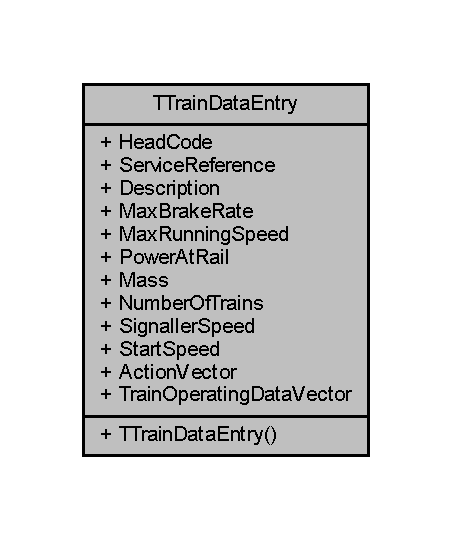
\includegraphics[width=217pt]{class_t_train_data_entry__coll__graph}
\end{center}
\end{figure}
\subsection*{Public Attributes}
\begin{DoxyCompactItemize}
\item 
\mbox{\Hypertarget{class_t_train_data_entry_aa1c7c0c8f2437744f49d7e2856180dd8}\label{class_t_train_data_entry_aa1c7c0c8f2437744f49d7e2856180dd8}} 
Ansi\+String {\bfseries Head\+Code}
\item 
\mbox{\Hypertarget{class_t_train_data_entry_aadf0846698c4d7d596c9280037834456}\label{class_t_train_data_entry_aadf0846698c4d7d596c9280037834456}} 
Ansi\+String {\bfseries Service\+Reference}
\item 
\mbox{\Hypertarget{class_t_train_data_entry_aea5870826c3c6815472e86d82b0c9fe7}\label{class_t_train_data_entry_aea5870826c3c6815472e86d82b0c9fe7}} 
Ansi\+String {\bfseries Description}
\item 
\mbox{\Hypertarget{class_t_train_data_entry_a3d7e696d79ee15cae196c0197fed3821}\label{class_t_train_data_entry_a3d7e696d79ee15cae196c0197fed3821}} 
double {\bfseries Max\+Brake\+Rate}
\item 
\mbox{\Hypertarget{class_t_train_data_entry_aaef868581a7c5383f70f119b1f551178}\label{class_t_train_data_entry_aaef868581a7c5383f70f119b1f551178}} 
double {\bfseries Max\+Running\+Speed}
\item 
\mbox{\Hypertarget{class_t_train_data_entry_a41d5f92deb8a429cad0e1dadf2727fe4}\label{class_t_train_data_entry_a41d5f92deb8a429cad0e1dadf2727fe4}} 
double {\bfseries Power\+At\+Rail}
\item 
\mbox{\Hypertarget{class_t_train_data_entry_a16d6c71abfab0a1ebd961fe3cd3edae7}\label{class_t_train_data_entry_a16d6c71abfab0a1ebd961fe3cd3edae7}} 
int {\bfseries Mass}
\item 
\mbox{\Hypertarget{class_t_train_data_entry_a977ccbe485d557d4c4a597f5de2251c4}\label{class_t_train_data_entry_a977ccbe485d557d4c4a597f5de2251c4}} 
int {\bfseries Number\+Of\+Trains}
\item 
\mbox{\Hypertarget{class_t_train_data_entry_a5ffd52b10fc56a29a823b918a40197e8}\label{class_t_train_data_entry_a5ffd52b10fc56a29a823b918a40197e8}} 
int {\bfseries Signaller\+Speed}
\item 
\mbox{\Hypertarget{class_t_train_data_entry_a573e640a04585cde4c5bbe2bced866d6}\label{class_t_train_data_entry_a573e640a04585cde4c5bbe2bced866d6}} 
int {\bfseries Start\+Speed}
\item 
\mbox{\Hypertarget{class_t_train_data_entry_a73872a2abaa9d09a3f392b4e6f725289}\label{class_t_train_data_entry_a73872a2abaa9d09a3f392b4e6f725289}} 
T\+Action\+Vector {\bfseries Action\+Vector}
\item 
\mbox{\Hypertarget{class_t_train_data_entry_a384ddee4ede5a1962011bdc0fc3c7587}\label{class_t_train_data_entry_a384ddee4ede5a1962011bdc0fc3c7587}} 
T\+Train\+Operating\+Data\+Vector {\bfseries Train\+Operating\+Data\+Vector}
\end{DoxyCompactItemize}


The documentation for this class was generated from the following file\+:\begin{DoxyCompactItemize}
\item 
Train\+Unit.\+h\end{DoxyCompactItemize}

\hypertarget{class_t_train_formatted_information}{}\section{T\+Train\+Formatted\+Information Class Reference}
\label{class_t_train_formatted_information}\index{T\+Train\+Formatted\+Information@{T\+Train\+Formatted\+Information}}


Contains all information for a single timetable entry for use in the formatted timetable.  




{\ttfamily \#include $<$Train\+Unit.\+h$>$}



Collaboration diagram for T\+Train\+Formatted\+Information\+:\nopagebreak
\begin{figure}[H]
\begin{center}
\leavevmode
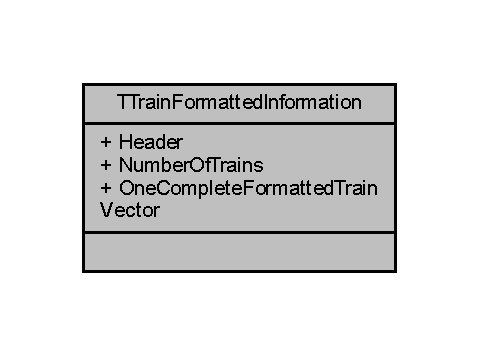
\includegraphics[width=230pt]{class_t_train_formatted_information__coll__graph}
\end{center}
\end{figure}
\subsection*{Public Attributes}
\begin{DoxyCompactItemize}
\item 
\mbox{\Hypertarget{class_t_train_formatted_information_a03b72f64d740876d99d1080b8d355441}\label{class_t_train_formatted_information_a03b72f64d740876d99d1080b8d355441}} 
Ansi\+String \mbox{\hyperlink{class_t_train_formatted_information_a03b72f64d740876d99d1080b8d355441}{Header}}
\begin{DoxyCompactList}\small\item\em description, mass, power, brake rate etc \end{DoxyCompactList}\item 
\mbox{\Hypertarget{class_t_train_formatted_information_a2f5bc8f1ff9b154a381660639c40dada}\label{class_t_train_formatted_information_a2f5bc8f1ff9b154a381660639c40dada}} 
int \mbox{\hyperlink{class_t_train_formatted_information_a2f5bc8f1ff9b154a381660639c40dada}{Number\+Of\+Trains}}
\begin{DoxyCompactList}\small\item\em number of repeats + 1 \end{DoxyCompactList}\item 
\mbox{\Hypertarget{class_t_train_formatted_information_a7ed8168782c7afd5f7b42b41f5515c8f}\label{class_t_train_formatted_information_a7ed8168782c7afd5f7b42b41f5515c8f}} 
T\+One\+Complete\+Formatted\+Train\+Vector \mbox{\hyperlink{class_t_train_formatted_information_a7ed8168782c7afd5f7b42b41f5515c8f}{One\+Complete\+Formatted\+Train\+Vector}}
\begin{DoxyCompactList}\small\item\em see above \end{DoxyCompactList}\end{DoxyCompactItemize}


\subsection{Detailed Description}
Contains all information for a single timetable entry for use in the formatted timetable. 

The documentation for this class was generated from the following file\+:\begin{DoxyCompactItemize}
\item 
Train\+Unit.\+h\end{DoxyCompactItemize}

\hypertarget{class_t_train_operating_data}{}\section{T\+Train\+Operating\+Data Class Reference}
\label{class_t_train_operating_data}\index{T\+Train\+Operating\+Data@{T\+Train\+Operating\+Data}}


Data for a specific train for use during operation.  




{\ttfamily \#include $<$Train\+Unit.\+h$>$}



Collaboration diagram for T\+Train\+Operating\+Data\+:\nopagebreak
\begin{figure}[H]
\begin{center}
\leavevmode
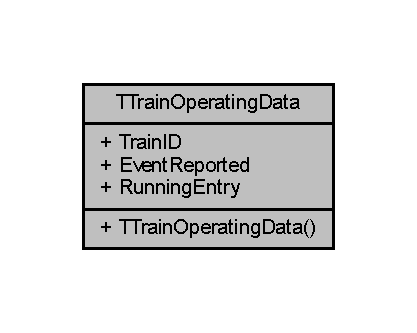
\includegraphics[width=200pt]{class_t_train_operating_data__coll__graph}
\end{center}
\end{figure}
\subsection*{Public Member Functions}
\begin{DoxyCompactItemize}
\item 
\mbox{\Hypertarget{class_t_train_operating_data_a0d7961667bbcdf20a744db7c1a2125af}\label{class_t_train_operating_data_a0d7961667bbcdf20a744db7c1a2125af}} 
\mbox{\hyperlink{class_t_train_operating_data_a0d7961667bbcdf20a744db7c1a2125af}{T\+Train\+Operating\+Data}} ()
\begin{DoxyCompactList}\small\item\em Constructor, values set to defaults. \end{DoxyCompactList}\end{DoxyCompactItemize}
\subsection*{Public Attributes}
\begin{DoxyCompactItemize}
\item 
\mbox{\Hypertarget{class_t_train_operating_data_aa75dba204a2655d41e74c42694e92b81}\label{class_t_train_operating_data_aa75dba204a2655d41e74c42694e92b81}} 
int {\bfseries Train\+ID}
\item 
\mbox{\Hypertarget{class_t_train_operating_data_afd7bc1b962e312062e0d27f0380e8c69}\label{class_t_train_operating_data_afd7bc1b962e312062e0d27f0380e8c69}} 
T\+Action\+Event\+Type {\bfseries Event\+Reported}
\item 
\mbox{\Hypertarget{class_t_train_operating_data_a9a46cddc0bed9cbbfff18b8909ae8047}\label{class_t_train_operating_data_a9a46cddc0bed9cbbfff18b8909ae8047}} 
T\+Running\+Entry {\bfseries Running\+Entry}
\end{DoxyCompactItemize}


\subsection{Detailed Description}
Data for a specific train for use during operation. 

The documentation for this class was generated from the following file\+:\begin{DoxyCompactItemize}
\item 
Train\+Unit.\+h\end{DoxyCompactItemize}

\hypertarget{class_t_utilities}{}\section{T\+Utilities Class Reference}
\label{class_t_utilities}\index{T\+Utilities@{T\+Utilities}}
\subsection*{Public Member Functions}
\begin{DoxyCompactItemize}
\item 
\mbox{\Hypertarget{class_t_utilities_a9ca62e05ace8e6c4c33d377c26c48e55}\label{class_t_utilities_a9ca62e05ace8e6c4c33d377c26c48e55}} 
Ansi\+String {\bfseries Date\+Time\+Stamp} ()
\item 
\mbox{\Hypertarget{class_t_utilities_a34bd6bb5305bc29afdf424f6d35a921c}\label{class_t_utilities_a34bd6bb5305bc29afdf424f6d35a921c}} 
Ansi\+String {\bfseries Time\+Stamp} ()
\item 
\mbox{\Hypertarget{class_t_utilities_ae1eddca13cc3c492839e131f40ec21c0}\label{class_t_utilities_ae1eddca13cc3c492839e131f40ec21c0}} 
void {\bfseries Call\+Log\+Pop} (int Caller)
\item 
\mbox{\Hypertarget{class_t_utilities_a100a392ac8eeb3955796954a5afade36}\label{class_t_utilities_a100a392ac8eeb3955796954a5afade36}} 
void {\bfseries File\+Diagnostics} (Ansi\+String Input)
\item 
\mbox{\Hypertarget{class_t_utilities_a06a211ebaa112f3fac0edc5b238ef876}\label{class_t_utilities_a06a211ebaa112f3fac0edc5b238ef876}} 
void {\bfseries Save\+File\+Bool} (std\+::ofstream \&Out\+File, bool Save\+Bool)
\item 
\mbox{\Hypertarget{class_t_utilities_a86ed634e8a9d7ca534a324954f4a7a2f}\label{class_t_utilities_a86ed634e8a9d7ca534a324954f4a7a2f}} 
void {\bfseries Save\+File\+Int} (std\+::ofstream \&Out\+File, int Save\+Int)
\item 
\mbox{\Hypertarget{class_t_utilities_a92b5adfb8ad3a937a8d208bfd90a5741}\label{class_t_utilities_a92b5adfb8ad3a937a8d208bfd90a5741}} 
void {\bfseries Save\+File\+Double} (std\+::ofstream \&Out\+File, double Save\+Double)
\item 
\mbox{\Hypertarget{class_t_utilities_a60531c6cb1a6a33dd71299d3a5b6cc21}\label{class_t_utilities_a60531c6cb1a6a33dd71299d3a5b6cc21}} 
void {\bfseries Save\+File\+String} (std\+::ofstream \&Out\+File, Ansi\+String Save\+String)
\item 
\mbox{\Hypertarget{class_t_utilities_a9a0ec4d0c686c71157c371d647824777}\label{class_t_utilities_a9a0ec4d0c686c71157c371d647824777}} 
bool {\bfseries Load\+File\+Bool} (std\+::ifstream \&In\+File)
\item 
\mbox{\Hypertarget{class_t_utilities_a84bf39701305cf4814377d178d0fec8c}\label{class_t_utilities_a84bf39701305cf4814377d178d0fec8c}} 
int {\bfseries Load\+File\+Int} (std\+::ifstream \&In\+File)
\item 
\mbox{\Hypertarget{class_t_utilities_ac970a0df84f5cb26ed962020b7dc2d6d}\label{class_t_utilities_ac970a0df84f5cb26ed962020b7dc2d6d}} 
double {\bfseries Load\+File\+Double} (std\+::ifstream \&In\+File)
\item 
\mbox{\Hypertarget{class_t_utilities_a0aac90f10a08736514da3b3e02129e1e}\label{class_t_utilities_a0aac90f10a08736514da3b3e02129e1e}} 
Ansi\+String {\bfseries Load\+File\+String} (std\+::ifstream \&In\+File)
\item 
\mbox{\Hypertarget{class_t_utilities_a1b39fffcd392bfb0f5a2ca393de3a6bb}\label{class_t_utilities_a1b39fffcd392bfb0f5a2ca393de3a6bb}} 
bool {\bfseries Check\+File\+Bool} (std\+::ifstream \&In\+File)
\item 
\mbox{\Hypertarget{class_t_utilities_a4d229af6e8943da1936bcbcc1c83846b}\label{class_t_utilities_a4d229af6e8943da1936bcbcc1c83846b}} 
bool {\bfseries Check\+File\+Int} (std\+::ifstream \&In\+File, int Lowest, int Highest)
\item 
\mbox{\Hypertarget{class_t_utilities_ab4b66aa7480fda73d554fe0bcca82b60}\label{class_t_utilities_ab4b66aa7480fda73d554fe0bcca82b60}} 
bool {\bfseries Check\+And\+Read\+File\+Int} (std\+::ifstream \&In\+File, int Lowest, int Highest, int \&Out\+Int)
\item 
\mbox{\Hypertarget{class_t_utilities_a5c7332a6b45894902f271f0ab9ab87db}\label{class_t_utilities_a5c7332a6b45894902f271f0ab9ab87db}} 
bool {\bfseries Check\+File\+Double} (std\+::ifstream \&In\+File)
\item 
\mbox{\Hypertarget{class_t_utilities_a7896a24d025c8164b2c8215944d072aa}\label{class_t_utilities_a7896a24d025c8164b2c8215944d072aa}} 
bool {\bfseries Check\+File\+String} (std\+::ifstream \&In\+File)
\item 
\mbox{\Hypertarget{class_t_utilities_a8bc6745e0433d55022e016b6551f04a0}\label{class_t_utilities_a8bc6745e0433d55022e016b6551f04a0}} 
bool {\bfseries Check\+File\+String\+Zero\+Delimiter} (std\+::ifstream \&In\+File)
\item 
\mbox{\Hypertarget{class_t_utilities_a6a03c1597e2cc5d71c2f88ac36f11363}\label{class_t_utilities_a6a03c1597e2cc5d71c2f88ac36f11363}} 
bool {\bfseries Check\+And\+Compare\+File\+String} (std\+::ifstream \&In\+File, Ansi\+String In\+String)
\item 
\mbox{\Hypertarget{class_t_utilities_a0a0ef5bf2fc74c0026f2a8bec4151d37}\label{class_t_utilities_a0a0ef5bf2fc74c0026f2a8bec4151d37}} 
bool {\bfseries Check\+And\+Read\+File\+String} (std\+::ifstream \&In\+File, Ansi\+String \&Out\+String)
\item 
\mbox{\Hypertarget{class_t_utilities_a2dfbe3d4ed11770bc1a902b51afdc10c}\label{class_t_utilities_a2dfbe3d4ed11770bc1a902b51afdc10c}} 
Ansi\+String {\bfseries Format96\+H\+H\+M\+M\+SS} (T\+Date\+Time Date\+Time)
\item 
\mbox{\Hypertarget{class_t_utilities_a6dc0e83b149563fdf43f068fd26cead8}\label{class_t_utilities_a6dc0e83b149563fdf43f068fd26cead8}} 
Ansi\+String {\bfseries Format96\+H\+H\+MM} (T\+Date\+Time Date\+Time)
\end{DoxyCompactItemize}
\subsection*{Public Attributes}
\begin{DoxyCompactItemize}
\item 
\mbox{\Hypertarget{class_t_utilities_a0fd0d8e0ec95309b508fd37fa541555e}\label{class_t_utilities_a0fd0d8e0ec95309b508fd37fa541555e}} 
bool {\bfseries Clock2\+Stopped}
\item 
\mbox{\Hypertarget{class_t_utilities_a3c2a72a2871d92ccaced9ab9f91d65c2}\label{class_t_utilities_a3c2a72a2871d92ccaced9ab9f91d65c2}} 
bool {\bfseries R\+H\+Signal\+Flag}
\item 
\mbox{\Hypertarget{class_t_utilities_ac9422864dc36c3d98ad952f10026c572}\label{class_t_utilities_ac9422864dc36c3d98ad952f10026c572}} 
int {\bfseries Screen\+Element\+Width}
\item 
\mbox{\Hypertarget{class_t_utilities_a45d9703729a28c2fb2638539fa909e81}\label{class_t_utilities_a45d9703729a28c2fb2638539fa909e81}} 
int {\bfseries Screen\+Element\+Height}
\item 
\mbox{\Hypertarget{class_t_utilities_acc7cd1d066ac7942ad6c1239b3c25eee}\label{class_t_utilities_acc7cd1d066ac7942ad6c1239b3c25eee}} 
std\+::ofstream {\bfseries Performance\+File}
\item 
\mbox{\Hypertarget{class_t_utilities_abf6c3e70d5fbf58720ff0d9f80de5bde}\label{class_t_utilities_abf6c3e70d5fbf58720ff0d9f80de5bde}} 
std\+::deque$<$ Ansi\+String $>$ {\bfseries Call\+Log}
\item 
\mbox{\Hypertarget{class_t_utilities_ace6be5cece5f2e271c0b85a9d2f51917}\label{class_t_utilities_ace6be5cece5f2e271c0b85a9d2f51917}} 
std\+::deque$<$ Ansi\+String $>$ {\bfseries Event\+Log}
\item 
\mbox{\Hypertarget{class_t_utilities_a89b8716bbc78332d40427ed688ce56bd}\label{class_t_utilities_a89b8716bbc78332d40427ed688ce56bd}} 
T\+Color {\bfseries cl\+Transparent}
\end{DoxyCompactItemize}


The documentation for this class was generated from the following files\+:\begin{DoxyCompactItemize}
\item 
C\+:/\+Programming work/railway development after v2.\+2.\+0/Utilities.\+h\item 
C\+:/\+Programming work/railway development after v2.\+2.\+0/Utilities.\+cpp\end{DoxyCompactItemize}

%--- End generated contents ---

% Index
\backmatter
\newpage
\phantomsection
\clearemptydoublepage
\addcontentsline{toc}{chapter}{Index}
\printindex

\end{document}
